% Options for packages loaded elsewhere
\PassOptionsToPackage{unicode}{hyperref}
\PassOptionsToPackage{hyphens}{url}
%
\documentclass[
]{book}
\usepackage{amsmath,amssymb}
\usepackage{iftex}
\ifPDFTeX
  \usepackage[T1]{fontenc}
  \usepackage[utf8]{inputenc}
  \usepackage{textcomp} % provide euro and other symbols
\else % if luatex or xetex
  \usepackage{unicode-math} % this also loads fontspec
  \defaultfontfeatures{Scale=MatchLowercase}
  \defaultfontfeatures[\rmfamily]{Ligatures=TeX,Scale=1}
\fi
\usepackage{lmodern}
\ifPDFTeX\else
  % xetex/luatex font selection
\fi
% Use upquote if available, for straight quotes in verbatim environments
\IfFileExists{upquote.sty}{\usepackage{upquote}}{}
\IfFileExists{microtype.sty}{% use microtype if available
  \usepackage[]{microtype}
  \UseMicrotypeSet[protrusion]{basicmath} % disable protrusion for tt fonts
}{}
\makeatletter
\@ifundefined{KOMAClassName}{% if non-KOMA class
  \IfFileExists{parskip.sty}{%
    \usepackage{parskip}
  }{% else
    \setlength{\parindent}{0pt}
    \setlength{\parskip}{6pt plus 2pt minus 1pt}}
}{% if KOMA class
  \KOMAoptions{parskip=half}}
\makeatother
\usepackage{xcolor}
\usepackage{color}
\usepackage{fancyvrb}
\newcommand{\VerbBar}{|}
\newcommand{\VERB}{\Verb[commandchars=\\\{\}]}
\DefineVerbatimEnvironment{Highlighting}{Verbatim}{commandchars=\\\{\}}
% Add ',fontsize=\small' for more characters per line
\usepackage{framed}
\definecolor{shadecolor}{RGB}{248,248,248}
\newenvironment{Shaded}{\begin{snugshade}}{\end{snugshade}}
\newcommand{\AlertTok}[1]{\textcolor[rgb]{0.94,0.16,0.16}{#1}}
\newcommand{\AnnotationTok}[1]{\textcolor[rgb]{0.56,0.35,0.01}{\textbf{\textit{#1}}}}
\newcommand{\AttributeTok}[1]{\textcolor[rgb]{0.13,0.29,0.53}{#1}}
\newcommand{\BaseNTok}[1]{\textcolor[rgb]{0.00,0.00,0.81}{#1}}
\newcommand{\BuiltInTok}[1]{#1}
\newcommand{\CharTok}[1]{\textcolor[rgb]{0.31,0.60,0.02}{#1}}
\newcommand{\CommentTok}[1]{\textcolor[rgb]{0.56,0.35,0.01}{\textit{#1}}}
\newcommand{\CommentVarTok}[1]{\textcolor[rgb]{0.56,0.35,0.01}{\textbf{\textit{#1}}}}
\newcommand{\ConstantTok}[1]{\textcolor[rgb]{0.56,0.35,0.01}{#1}}
\newcommand{\ControlFlowTok}[1]{\textcolor[rgb]{0.13,0.29,0.53}{\textbf{#1}}}
\newcommand{\DataTypeTok}[1]{\textcolor[rgb]{0.13,0.29,0.53}{#1}}
\newcommand{\DecValTok}[1]{\textcolor[rgb]{0.00,0.00,0.81}{#1}}
\newcommand{\DocumentationTok}[1]{\textcolor[rgb]{0.56,0.35,0.01}{\textbf{\textit{#1}}}}
\newcommand{\ErrorTok}[1]{\textcolor[rgb]{0.64,0.00,0.00}{\textbf{#1}}}
\newcommand{\ExtensionTok}[1]{#1}
\newcommand{\FloatTok}[1]{\textcolor[rgb]{0.00,0.00,0.81}{#1}}
\newcommand{\FunctionTok}[1]{\textcolor[rgb]{0.13,0.29,0.53}{\textbf{#1}}}
\newcommand{\ImportTok}[1]{#1}
\newcommand{\InformationTok}[1]{\textcolor[rgb]{0.56,0.35,0.01}{\textbf{\textit{#1}}}}
\newcommand{\KeywordTok}[1]{\textcolor[rgb]{0.13,0.29,0.53}{\textbf{#1}}}
\newcommand{\NormalTok}[1]{#1}
\newcommand{\OperatorTok}[1]{\textcolor[rgb]{0.81,0.36,0.00}{\textbf{#1}}}
\newcommand{\OtherTok}[1]{\textcolor[rgb]{0.56,0.35,0.01}{#1}}
\newcommand{\PreprocessorTok}[1]{\textcolor[rgb]{0.56,0.35,0.01}{\textit{#1}}}
\newcommand{\RegionMarkerTok}[1]{#1}
\newcommand{\SpecialCharTok}[1]{\textcolor[rgb]{0.81,0.36,0.00}{\textbf{#1}}}
\newcommand{\SpecialStringTok}[1]{\textcolor[rgb]{0.31,0.60,0.02}{#1}}
\newcommand{\StringTok}[1]{\textcolor[rgb]{0.31,0.60,0.02}{#1}}
\newcommand{\VariableTok}[1]{\textcolor[rgb]{0.00,0.00,0.00}{#1}}
\newcommand{\VerbatimStringTok}[1]{\textcolor[rgb]{0.31,0.60,0.02}{#1}}
\newcommand{\WarningTok}[1]{\textcolor[rgb]{0.56,0.35,0.01}{\textbf{\textit{#1}}}}
\usepackage{longtable,booktabs,array}
\usepackage{calc} % for calculating minipage widths
% Correct order of tables after \paragraph or \subparagraph
\usepackage{etoolbox}
\makeatletter
\patchcmd\longtable{\par}{\if@noskipsec\mbox{}\fi\par}{}{}
\makeatother
% Allow footnotes in longtable head/foot
\IfFileExists{footnotehyper.sty}{\usepackage{footnotehyper}}{\usepackage{footnote}}
\makesavenoteenv{longtable}
\usepackage{graphicx}
\makeatletter
\def\maxwidth{\ifdim\Gin@nat@width>\linewidth\linewidth\else\Gin@nat@width\fi}
\def\maxheight{\ifdim\Gin@nat@height>\textheight\textheight\else\Gin@nat@height\fi}
\makeatother
% Scale images if necessary, so that they will not overflow the page
% margins by default, and it is still possible to overwrite the defaults
% using explicit options in \includegraphics[width, height, ...]{}
\setkeys{Gin}{width=\maxwidth,height=\maxheight,keepaspectratio}
% Set default figure placement to htbp
\makeatletter
\def\fps@figure{htbp}
\makeatother
\setlength{\emergencystretch}{3em} % prevent overfull lines
\providecommand{\tightlist}{%
  \setlength{\itemsep}{0pt}\setlength{\parskip}{0pt}}
\setcounter{secnumdepth}{5}
\usepackage{booktabs}
\usepackage{longtable}
\usepackage{array}
\usepackage{multirow}
\usepackage{wrapfig}
\usepackage{float}
\usepackage{colortbl}
\usepackage{pdflscape}
\usepackage{tabu}
\usepackage{threeparttable}
\usepackage{threeparttablex}
\usepackage[normalem]{ulem}
\usepackage{makecell}
\usepackage{xcolor}
\usepackage{fvextra}


\DefineVerbatimEnvironment{Highlighting}{Verbatim}{breaklines,commandchars=\\\{\}}
\usepackage[top=3cm, bottom=3cm, left=2cm, right=2cm, a4paper]{geometry}
\usepackage{titling}
\usepackage{pdfpages}
\usepackage{multirow}
\usepackage{multicol}
\pretitle{\begin{center}
\includepdf{images1/logo-uel.png}}
\posttitle{\end{center}}
\usepackage{atbegshi}% http://ctan.org/pkg/atbegshi
\AtBeginDocument{\AtBeginShipoutNext{\AtBeginShipoutDiscard}}
\AtBeginDocument{\renewcommand{\chaptername}{Módulo}}
\AtBeginDocument{\renewcommand{\contentsname}{Índice}}
\usepackage{booktabs}
\usepackage{longtable}
\usepackage{array}
\usepackage{multirow}
\usepackage{wrapfig}
\usepackage{float}
\usepackage{colortbl}
\usepackage{pdflscape}
\usepackage{tabu}
\usepackage{threeparttable}
\usepackage{threeparttablex}
\usepackage[normalem]{ulem}
\usepackage{makecell}
\usepackage{xcolor}
\ifLuaTeX
  \usepackage{selnolig}  % disable illegal ligatures
\fi
\usepackage[]{natbib}
\bibliographystyle{plainnat}
\IfFileExists{bookmark.sty}{\usepackage{bookmark}}{\usepackage{hyperref}}
\IfFileExists{xurl.sty}{\usepackage{xurl}}{} % add URL line breaks if available
\urlstyle{same}
\hypersetup{
  hidelinks,
  pdfcreator={LaTeX via pandoc}}

\title{UNIVERSIDADE ESTADUAL DE LONDRINA\\
CCE - Centro de Ciências Exatas\\
DSTA - Departamento de Estatística\\
Apostila de Estatística\\
Prof.~M.e Eng. Felinto Junior Da Costa}
\author{}
\date{\vspace{-2.5em}Londrina, 10 de agosto de 2023.}

\begin{document}
\maketitle

{
\setcounter{tocdepth}{1}
\tableofcontents
}
\hypertarget{section}{%
\chapter*{}\label{section}}
\addcontentsline{toc}{chapter}{}

\hypertarget{introduuxe7uxe3o-histuxf3rica-da-estatuxedstica}{%
\chapter{Introdução histórica da estatística}\label{introduuxe7uxe3o-histuxf3rica-da-estatuxedstica}}

\hypertarget{primeiros-levantamentos-estudos-e-publicauxe7uxf5es-demografia-e-aritmuxe9tica-poluxedtica}{%
\section{Primeiros levantamentos, estudos e publicações \& Demografia e aritmética política}\label{primeiros-levantamentos-estudos-e-publicauxe7uxf5es-demografia-e-aritmuxe9tica-poluxedtica}}

1086

\hfill\break

O \emph{Domesday Book} \href{http://www.nationalarchives.gov.uk/education/resources/domesday-book/}{(link)}
foi encomendado em dezembro de 1085 por Guilherme, o Conquistador (\emph{King William I}), que invadiu a Inglaterra em 1066.

O primeiro esboço foi concluído em agosto de 1086 e continha registros de 13.418 assentamentos nos condados ingleses ao sul dos rios Ribble e Tees (a fronteira com a Escócia) com informações sobre terras, proprietários, uso da terra, empregados e animais cujo propósito básico era fundamentar a taxação (Figura \ref{fig:figA1}).

\hfill\break

\begin{figure}

{\centering 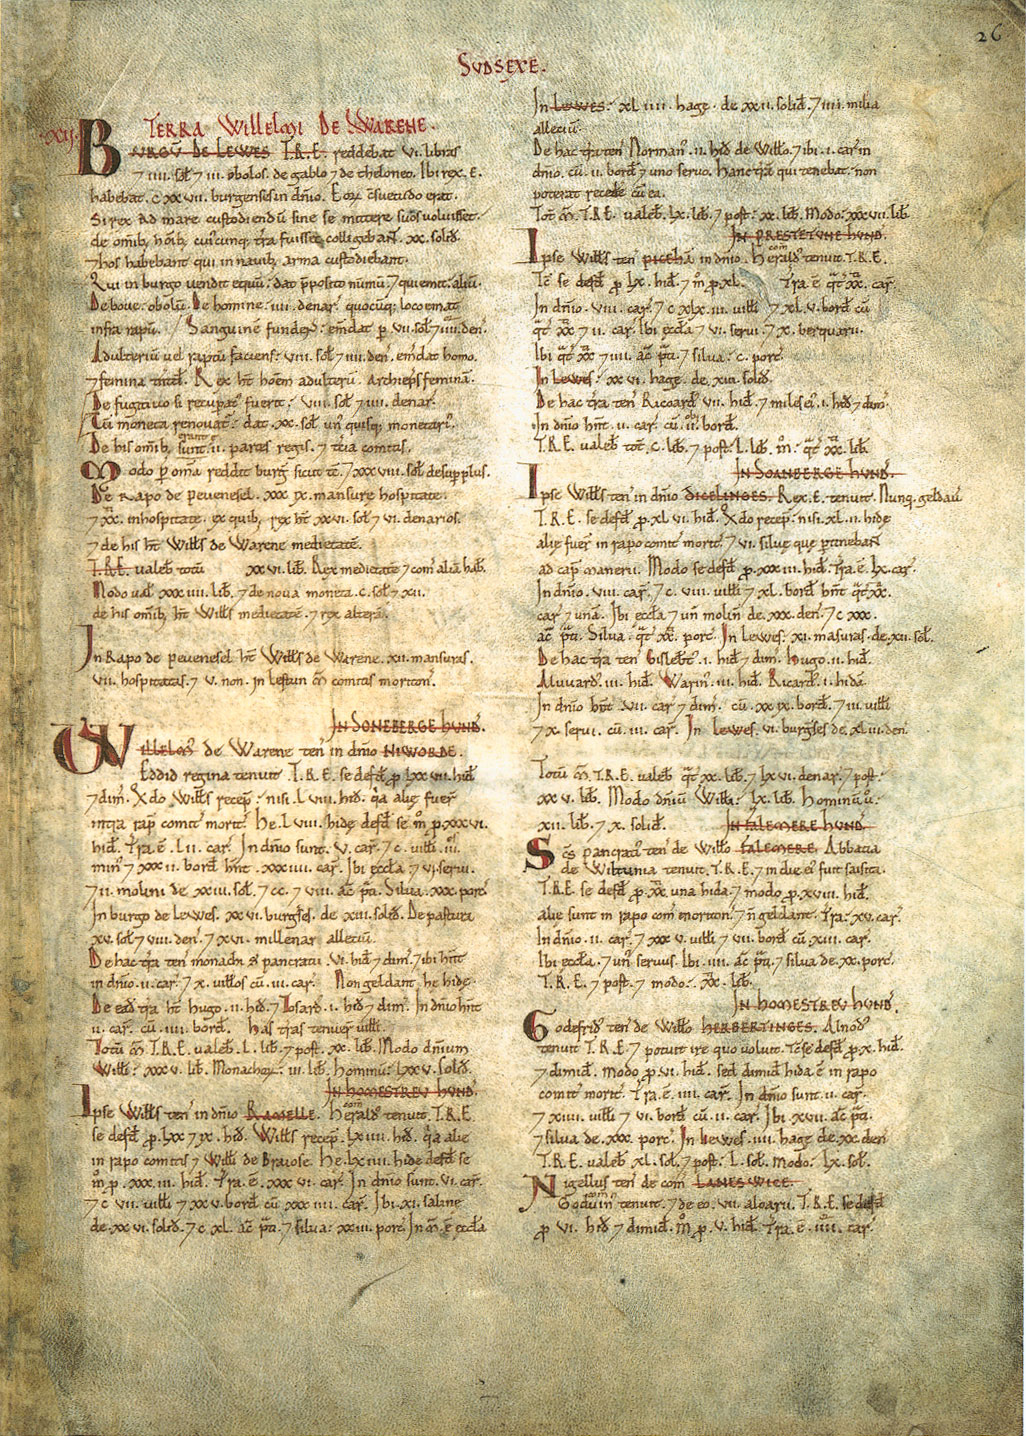
\includegraphics[width=0.75\linewidth]{images1/domesday} 

}

\caption{Domesday Book}\label{fig:figA1}
\end{figure}

\hfill\break

1602

\hfill\break

O dramaturgo inglês William Shakespeare usou a palavra \textbf{statists} (estadistas e, portanto, num sentido não relacionado com números ou matemática) no diálogo da Cena II de Hamlet \href{http://shakespeare.mit.edu/hamlet/full.html}{(link)}.

\hfill\break

\begin{quote}
``Hamlet:
Cercado assim por tantas vilanias, mesmo antes de eu poder dizer o prólogo, representava o cérebro.
Sentei-me e escrevi com capricho nova carta. Já pensei, como os nossos estadistas, que é feio escrever bem, tendo insistido, até, em desaprendê-lo; mas, nessa hora muito bom me foi isso. Quererias saber
qual o conteúdo da mensagem?{[}\ldots{]}''
\end{quote}

\hfill\break

1603

\hfill\break

O negociante inglês John Graunt (1620-1674) substituiu a crença pela evidência em \emph{Natural and Political Observations Mentioned in a Following Index and Made upon the Bills of Mortality} (Observações naturais e políticas feitas sobre as notas de mortalidade).

Nesse trabalho, realizado com dados coletados das paróquias de Londres entre 1604 e 1660, Graunt tirou as seguintes conclusões: que havia maior nascimento de crianças do sexo masculino, mas havia distribuição aproximadamente igual de ambos os sexos na população geral; alta mortalidade nos primeiros anos de vida; maior mortalidade nas zonas urbanas em relação às zonas rurais (Figura \ref{fig:figA2}).

\hfill\break

\begin{figure}

{\centering 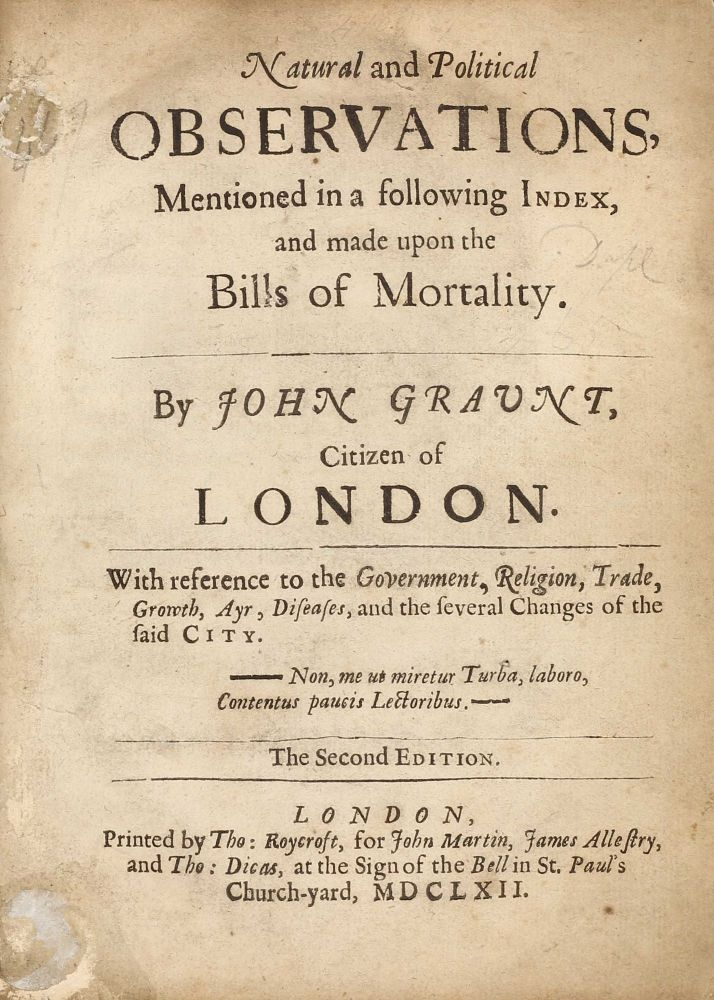
\includegraphics[width=0.75\linewidth]{images1/graunt} 

}

\caption{Natural and Political Observations Mentioned in a Following Index and Made upon the Bills of Mortality (ed. de 1662)}\label{fig:figA2}
\end{figure}

\hfill\break

1660

\hfill\break

Herman Conring (1606-1681), professor de filosofia, medicina e política da Universidade de Helmstadt (atual Alemanha), criou um curso de Ciência política em 1660, que descrevia e examinava as questões fundamentais do Estado. Nele a \textbf{estatística} passou a ser considerada como uma disciplina autônoma que tinha por objetivo a descrição das coisas do Estado.

\hfill\break

1687

\hfill\break

Em 1687 o economista e filósofo inglês William Petty (1623-1687) publicou \emph{Several Essays on Political Arithmetic} (Vários ensaios sobre aritmética política), sugerindo ao governo inglês a criação de um departamento para registro de \textbf{estatísticas} vitais (Figura \ref{fig:figA3}).

\hfill\break

\begin{figure}

{\centering 
\includegraphics[width=0.75\linewidth]{images1/petty} 

}

\caption{Several Essays in Political Arithmetick (ed. de 1699)}\label{fig:figA3}
\end{figure}

\hfill\break

O Capitão John Graunt e William Petty instituiram na Inglaterra um novo ramo de estudos denominado de \emph{Political arithmetic} (Aritmética política)

\hfill\break

1693

\hfill\break

O matemático e astrônomo inglês Edmond Halley (1656-1742) construiu em 1693, baseado em dados coletados na cidade (à época) alemã de Bresláu, uma \emph{Life Table} (Tábua de sobrevivência), um estudo que analisa as probabilidades de sobrevivência e morte em relação à idade (Figura \ref{fig:figA4}).

\hfill\break

\begin{figure}

{\centering 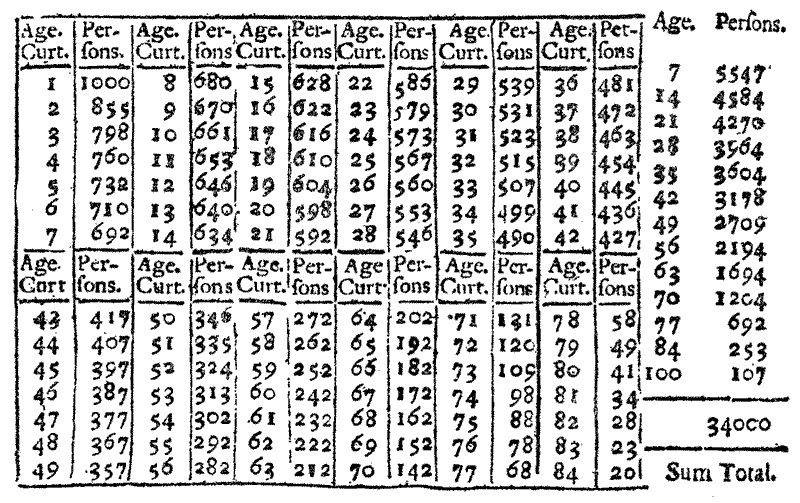
\includegraphics[width=0.75\linewidth]{images1/halley} 

}

\caption{Halley’s life table (1693)}\label{fig:figA4}
\end{figure}

\hfill\break

1749

\hfill\break

Com um sentido não relacionado com números ou matemática, a palavra \textbf{estatística} parece ter sido proposta pela primeira vez no século XVII, pelo historiador e professor alemão (à época Transilvânia) Martin Schmeitzel (1679-1747) da Universidade de Jena e, posteriormente adotada por seu aluno, (igualmente) historiador e jurista Gottfried Achenwall (1719-1772) em 1749, em \emph{Abriß der neuen Staatswissenschaft der vornehmen Europäischen Reiche und Republiken} (Esboço da nova ciência política dos nobres impérios europeus e repúblicas, Figura \ref{fig:figA5}).

\hfill\break

\begin{figure}

{\centering 
\includegraphics[width=0.75\linewidth]{images1/gottfried} 

}

\caption{Abriß der neuen Staatswissenschaft der vornehmen Europäischen Reiche und Republiken (1749)}\label{fig:figA5}
\end{figure}

\hfill\break

1771

\hfill\break

William Hooper usou a palavra \textbf{estatística} em sua tradução de \emph{The Elements of Universal Erudition}(Elementos da Erudição Universal) escrita por Jacob Friedrich Freiherr von Bielfeld (1717-1770).

Nesse livro, a \textbf{estatística} foi definida como a ciência que nos ensina o arranjo político de todos os estados modernos do mundo conhecido (mais uma veznum sentido não associado a números ou matemática, Figura \ref{fig:figA6}).

\hfill\break

\begin{figure}

{\centering 
\includegraphics[width=0.75\linewidth]{images1/hooper} 

}

\caption{The Elements of Universal Erudition  (1771)}\label{fig:figA6}
\end{figure}

\hfill\break

1790

\hfill\break

O jurista e político escocês John Sinclair propôs que se realizasse uma detalhada pesquisa em 938 paróquias para elucidar a história natural e política de seu país (\emph{Statistics Accounts}). Essa pesquisa fazia parte de um projeto muito mais ousado: \emph{The Pyramid of Statistical Enquiry} (A Pirâmide da Pesquisa Estatística, Figura \ref{fig:figA7}).

\hfill\break

\begin{figure}

{\centering 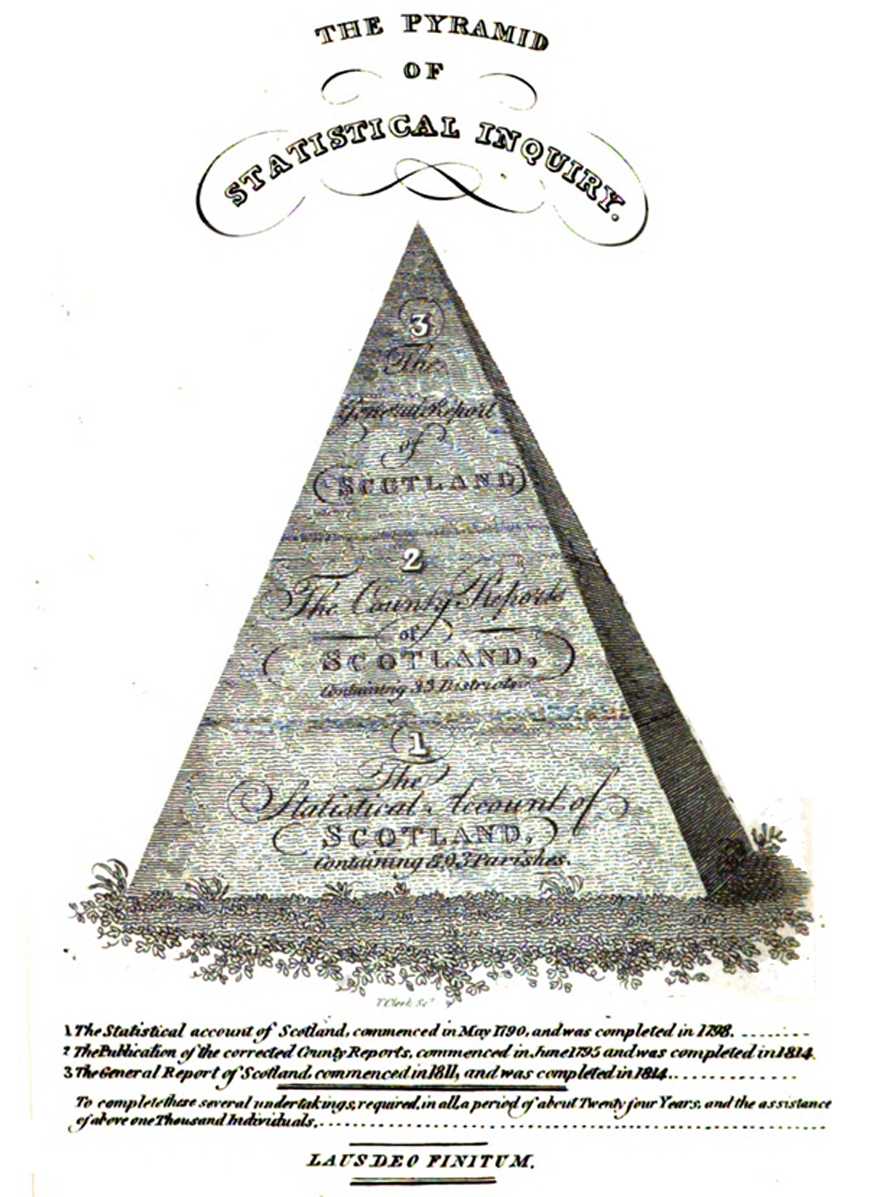
\includegraphics[width=0.75\linewidth]{images1/sinclair} 

}

\caption{The Pyramid of Statistical Enquiry  (1814)}\label{fig:figA7}
\end{figure}

\hfill\break

1854

\hfill\break
O médico inglês (considerado por alguns como o ``pai'' da epidemiologia moderna) John Snow (1813-1858) estudou a dispersão espacial dos casos de cólera em Londres e concluiu que sua causa residia na contaminação da água consumida (poço localizado na \emph{Broad Street}, no distrito do \emph{Soho}): \emph{Report to the Cholera Outbreak in the Parish of St.~James, Westminster during the Autumn of 1854} (Relatório sobre o surto de cólera na paróquia de St.~James, Westminster durante o outono de 1854, Figura \ref{fig:figA8}).

\hfill\break

\begin{figure}

{\centering 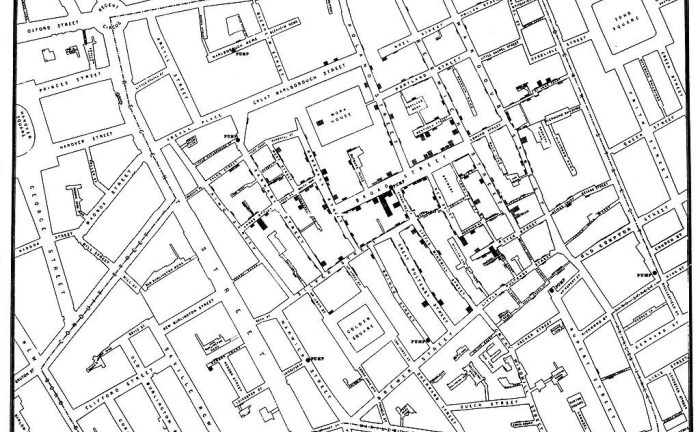
\includegraphics[width=0.75\linewidth]{images1/london-1854-snow} 

}

\caption{Mapa dos casos de cólera (1854)}\label{fig:figA8}
\end{figure}

\hypertarget{visualizauxe7uxe3o-de-dados-estudos-e-primeiras-publicauxe7uxf5es}{%
\section{Visualização de dados \& Estudos e primeiras publicações}\label{visualizauxe7uxe3o-de-dados-estudos-e-primeiras-publicauxe7uxf5es}}

1765

\hfill\break

O teólogo e filósofo inglês Joseph Priestley (1733-1804) introduziu como inovação os primeiros gráficos com linha temporal, em que barras individuais eram usadas para visualizar o tempo de vida de uma pessoa e o todo pode ser usado para comparar a expectativa de vida de várias pessoas (Figura \ref{fig:figA9}).

\hfill\break

\begin{figure}

{\centering 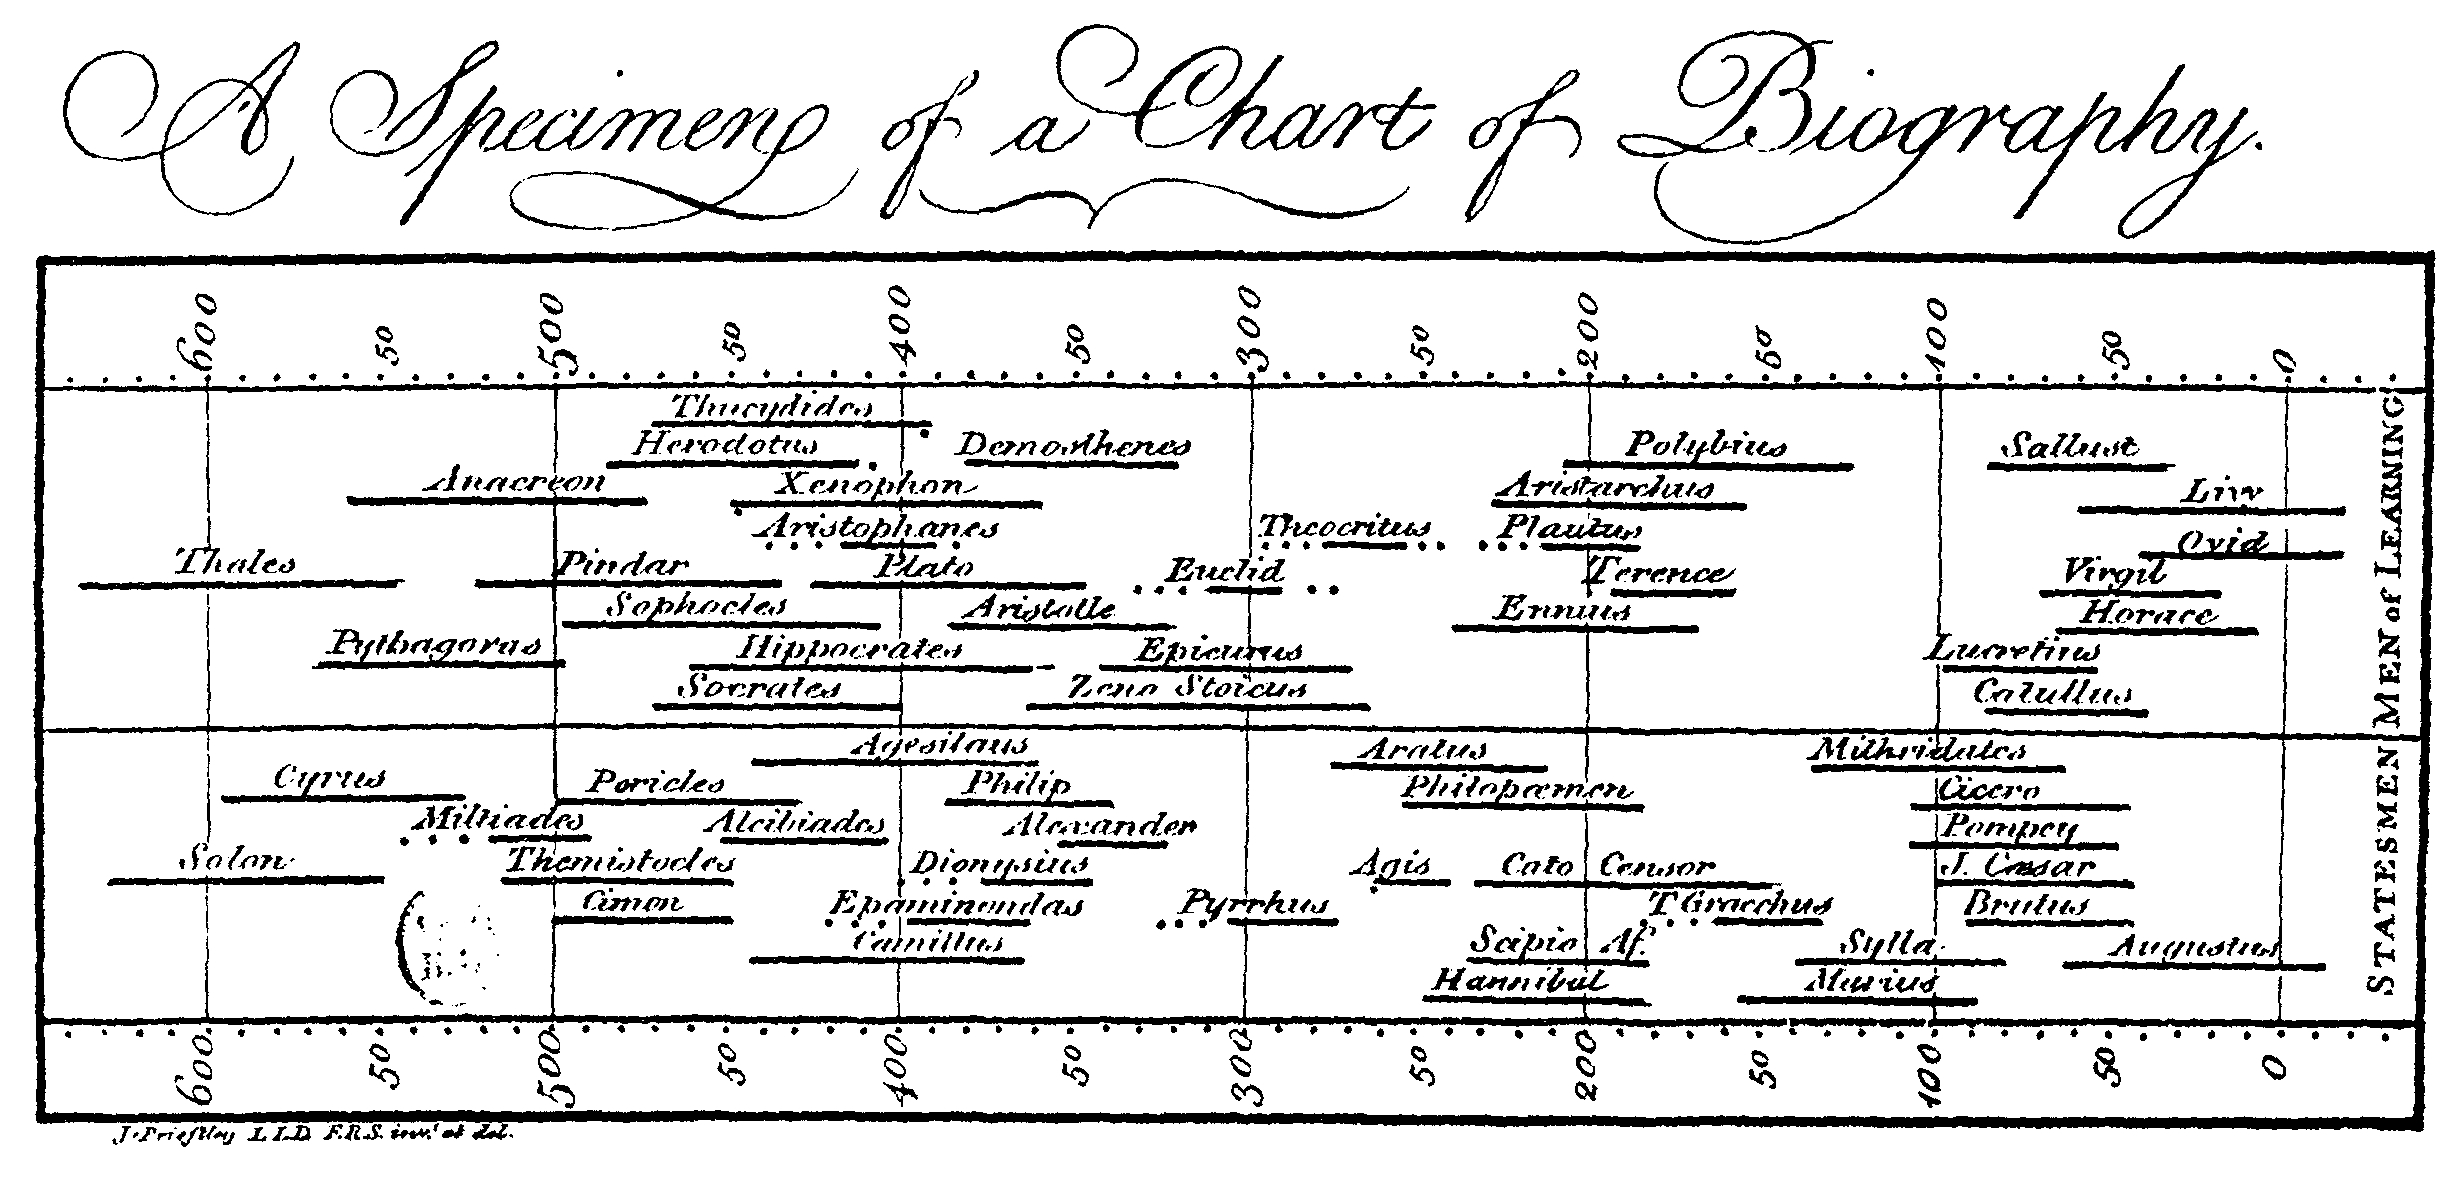
\includegraphics[width=0.75\linewidth]{images1/priestley-timechart-1765} 

}

\caption{Expectativa de vida de diversas pessoas (1765)}\label{fig:figA9}
\end{figure}

\hfill\break

1786

\hfill\break

O engenheiro e economista escocês William Playfair (1759-1823) é considerado comumente como fundador dos métodos gráficos para apresentação de estatísticas. Playfair concebeu vários tipos de diagramas para visualização de dados:

\begin{itemize}
\tightlist
\item
  em 1786, o gráfico de barras (Figura \ref{fig:figA10}); e,
\item
  em 1801, o gráfico de setores (Figura \ref{fig:figA11}).
\end{itemize}

\hfill\break

\begin{figure}

{\centering 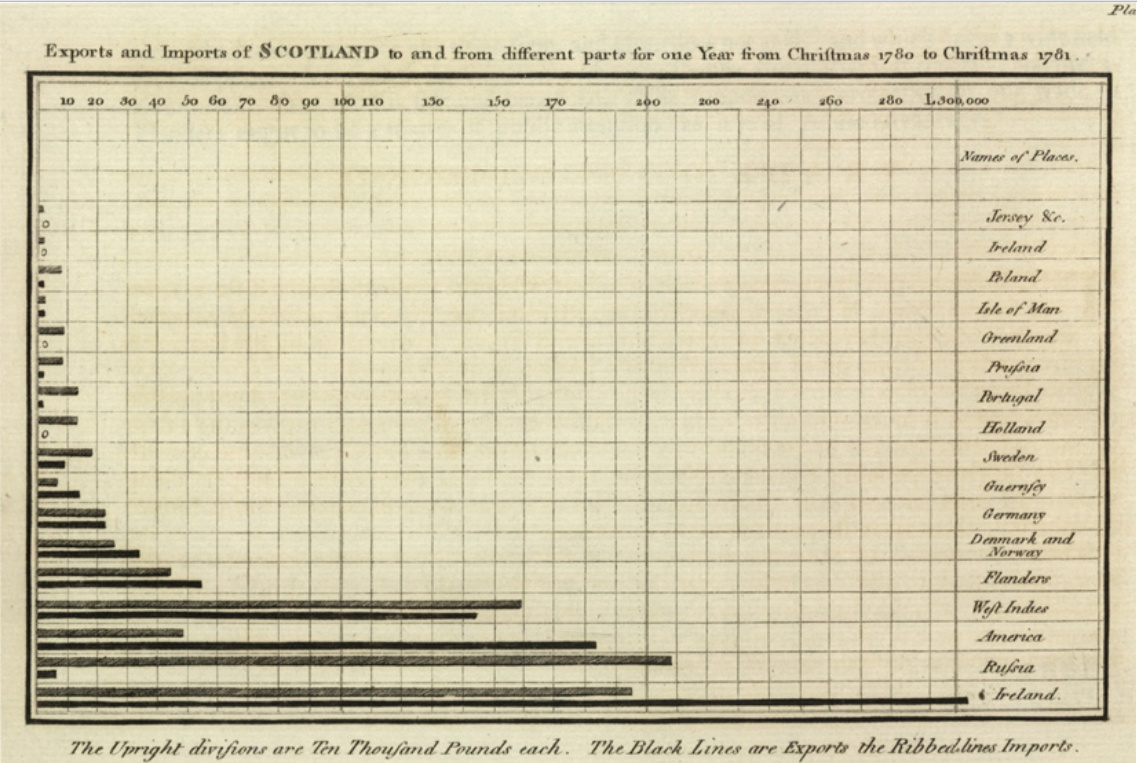
\includegraphics[width=0.75\linewidth]{images1/playfair-barchart-1786} 

}

\caption{Commercial and Political Atlas (Atlas Comercial e Político de 1786): cada barra representa as exportações e importações da Escócia para 17 países em 1781}\label{fig:figA10}
\end{figure}

\hfill\break

\begin{figure}

{\centering 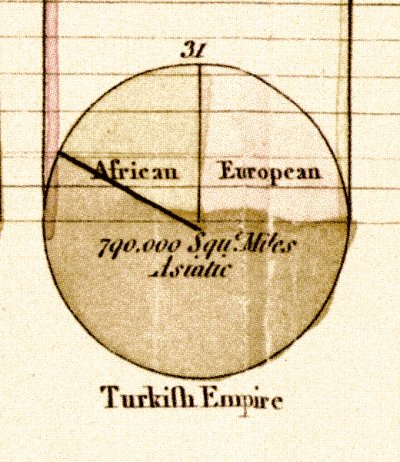
\includegraphics[width=0.75\linewidth]{images1/playfair-piechart-1801} 

}

\caption{Statistical Breviary (Breviário Estatístico de 1801): proporção da extensão do Império Turco em diferentes regiões do mundo: Asia, Europa e África, antes de 1789}\label{fig:figA11}
\end{figure}

\hfill\break

1856

\hfill\break

A enfermeira inglesa Florence Nightingale (1820-1910) conduziu um trabalho pioneiro ao chegar no hospital militar britânico na Turquia em 1856, estabelecendo uma ordem e um método muito necessários aos registros médicos estatísticos e que indicaram serem as precárias práticas sanitárias o culpado da alta mortalidade \href{https://www.york.ac.uk/depts/maths/histstat/small.htm}{(link)} , Figuras \ref{fig:figA12} e \ref{fig:figA13}.

\hfill\break

\begin{figure}

{\centering 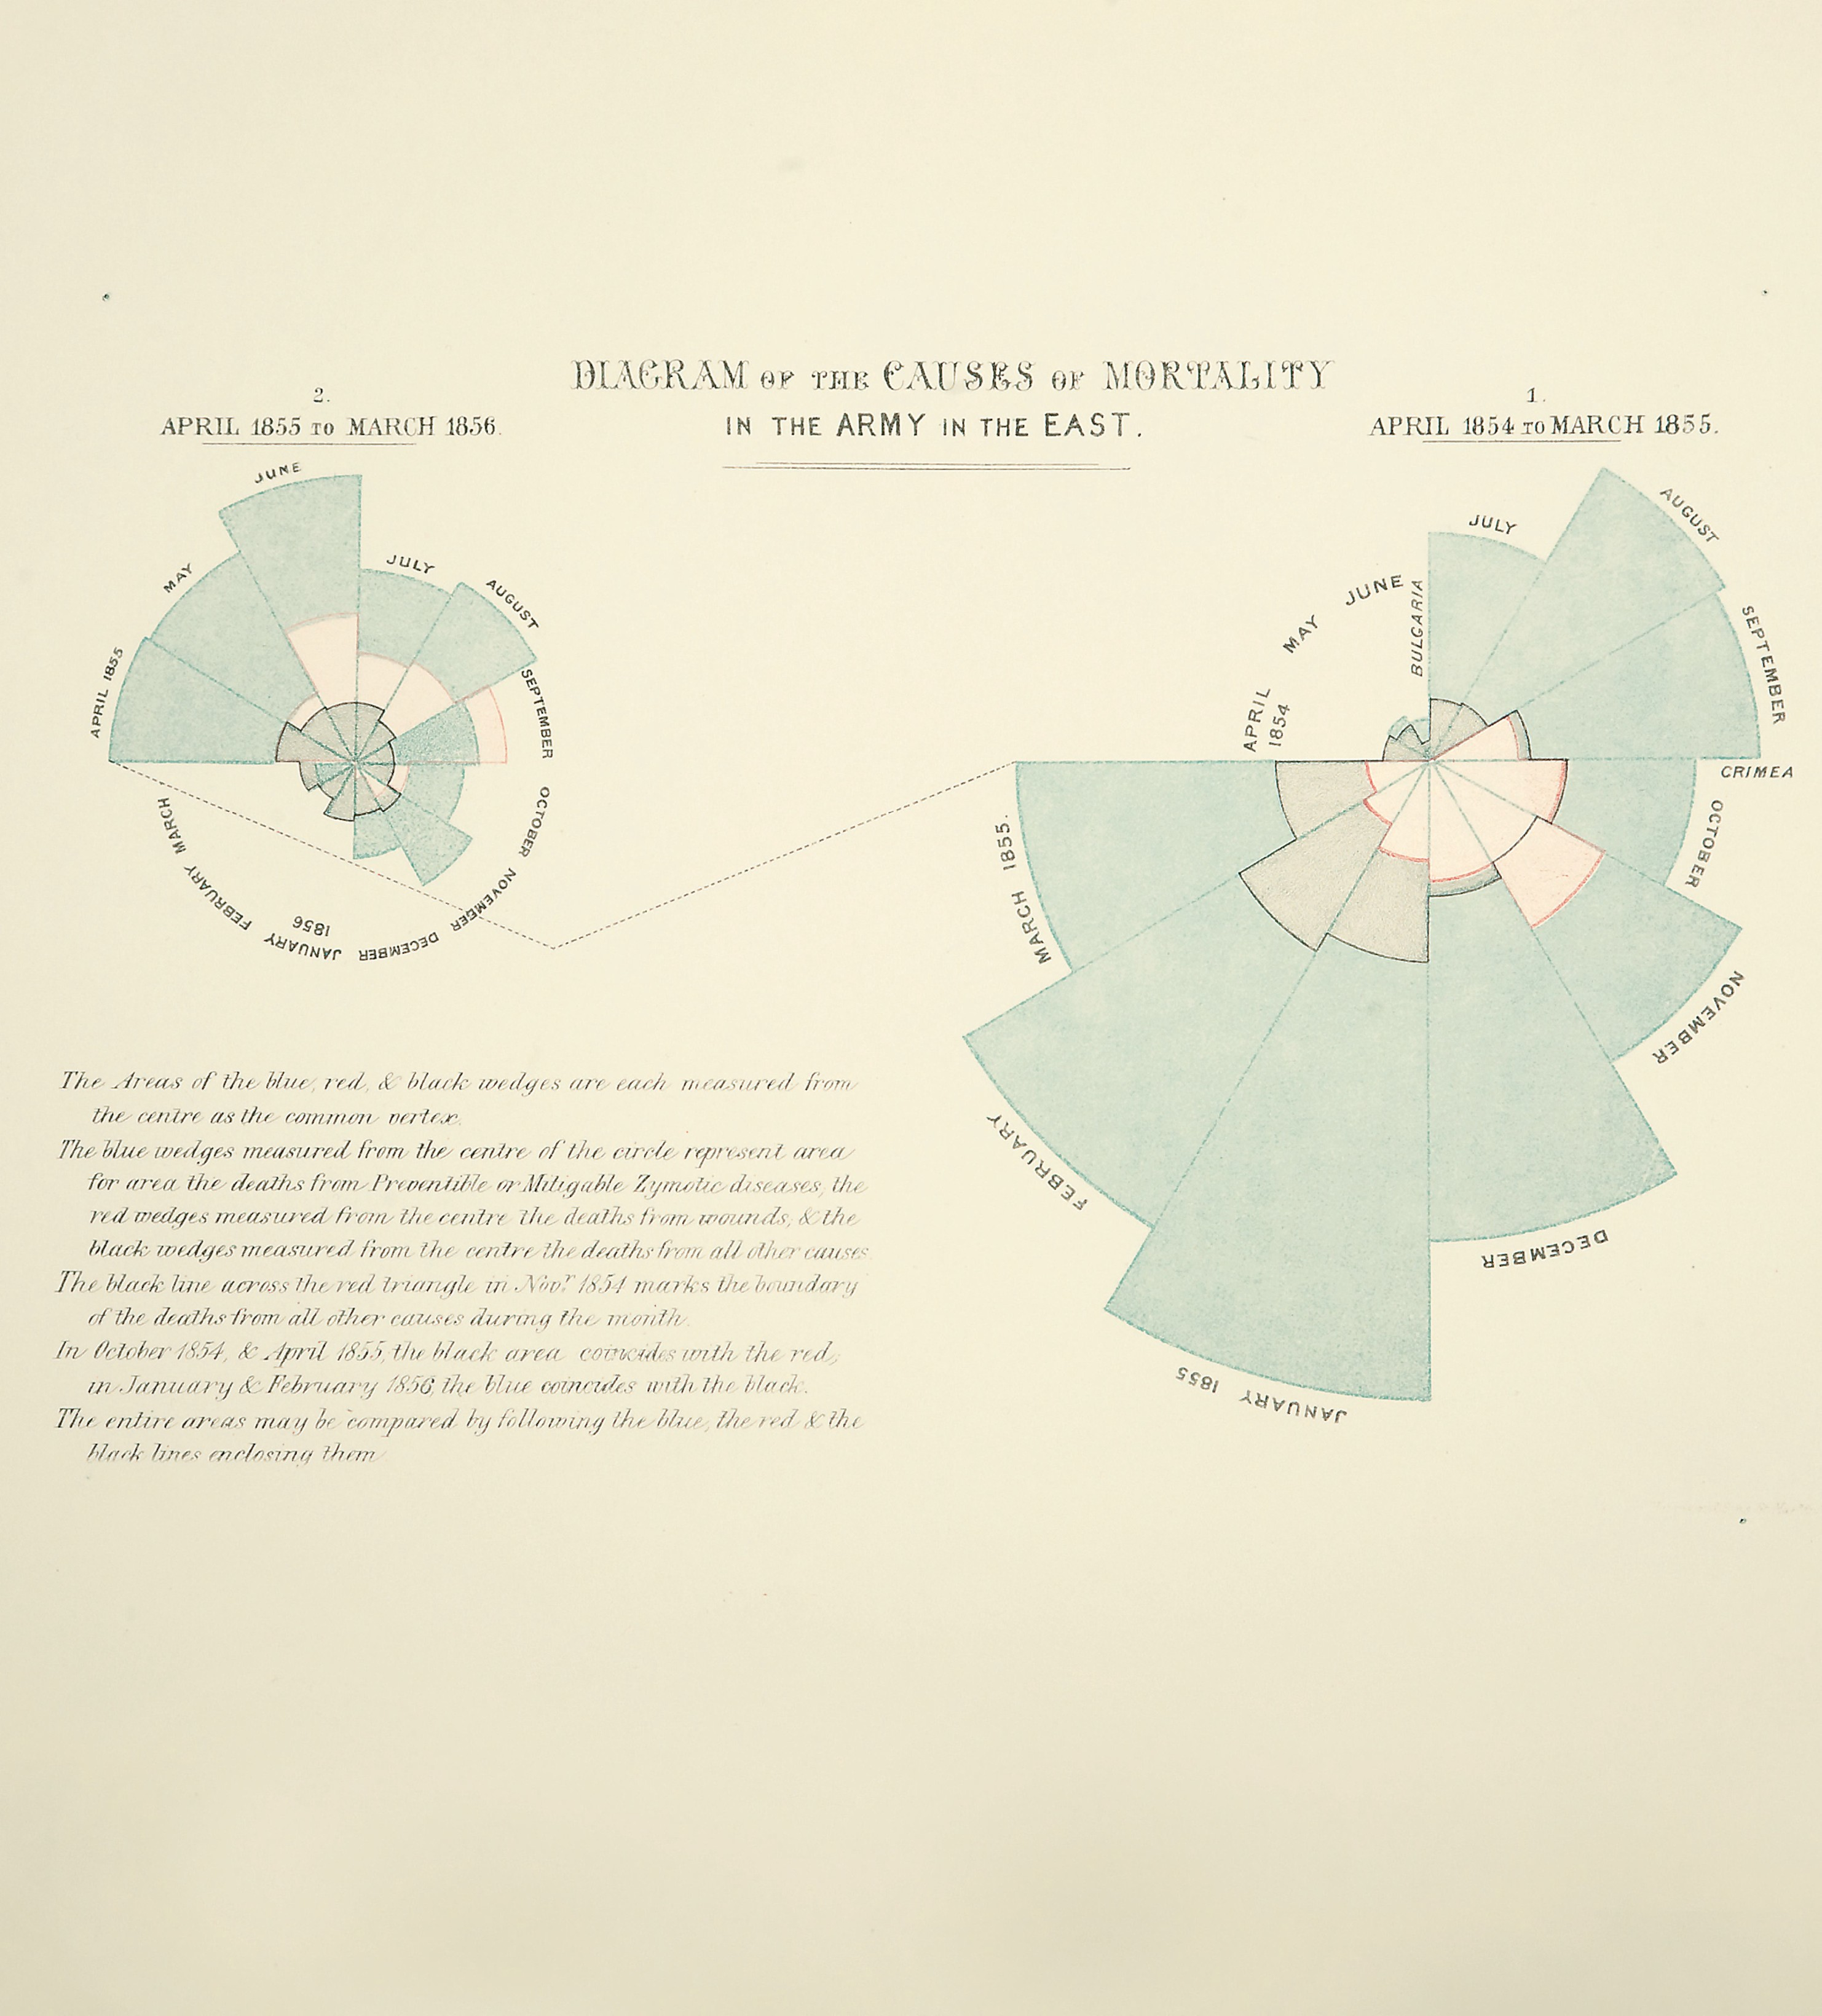
\includegraphics[width=0.75\linewidth]{images1/florence-rose-diagram} 

}

\caption{Esse diagrama (coxcomb) feito durante a Guerra da Crimeia foi dividido igualmente em 12 setores, representando os meses do ano, com a área sombreada do setor  de cada mês proporcional à taxa de mortalidade naquele mês. Seu sombreamento com código de cores indicava a causa da morte em cada área do diagrama}\label{fig:figA12}
\end{figure}

\hfill\break

\begin{figure}

{\centering 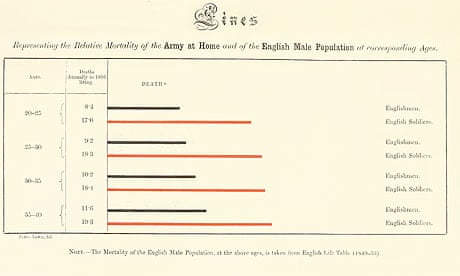
\includegraphics[width=0.75\linewidth]{images1/florence-barr} 

}

\caption{Gráfico de barras de Florence Nightingale mostrando as diferenças de mortalidade entre soldados britânicos e a população masculina inglesa geral (civis)}\label{fig:figA13}
\end{figure}

\hfill\break

\hypertarget{nomes-notuxe1veis}{%
\section{Nomes notáveis}\label{nomes-notuxe1veis}}

Karl Pearson (1857-1936) é amplamente considerado o fundador da disciplina moderna de \textbf{estatística}, e também é famoso como um filósofo da ciência, como escritor sobre o darwinismo social e como um dos principais impulsionadores para instalar a eugenia como a ciência social chave. Uma breve biografia de cada um dos pesquisadores a seguir relacionados pode ser obtida em: \href{http://www-history.mcs.st-andrews.ac.uk/BiogIndex.html}{(link)}.

\hfill\break

\begin{itemize}
\tightlist
\item
  Niccolò Fontana Tartaglia (Veneza à época, hoje Itália: 1499-1557)
\item
  Girolamo Cardano (Pávia à época, hoje Itália: 1501-1576)
\item
  Galileu Galilei (Florença à época, hoje Itália: 1564-1642)
\item
  Pierre de Fermat (França: 1607-1665)
\item
  Blaise Pascal (França: 1623-1662)
\item
  Jakob Bernoulli (Suíça: 1655-1705)
\item
  Abrahan de Moivre (França: 1667-1754)
\item
  Thomas Bayes (Inglaterra: 1702-1761)
\item
  Pierre-Simon Laplace (França: 1749-1827)
\item
  Johann Carl Friedrich Gauss (Alemanha: 1777-1856)
\item
  Lambert Adolphe Jacques Quételet (França à época, hoje Bélgica: 1796-1874)
\item
  Pafnuti Lvovitch Chebyshev (Rússia: 1821-1894)
\item
  Francis Galton (Inglaterra: 1822-1911)
\item
  Wilhelm Lexis (Alemanha: 1837-1914)
\item
  Thorvald Nicolai Thiele (Dinamarca: 1838-1910)
\item
  Friedrich Robert Helmert (Saxônia: 1843-1917)
\item
  Francis Ysidro Edgeworth (Inglaterra: 1845-1926)
\item
  James Douglas Hamilton Dickson (Escócia: 1849-1931)
\item
  Andrei Andreyevich Markov (Rússia: 1856-1922)
\item
  Aleksandr Mikhailovich Lyapunov (Rússia: 1857-1918)
\item
  Walter Frank Raphael Weldon (Inglaterra: 1860-1906)
\item
  Karl Pearson (Inglaterra: 1857-1936)
\item
  William Seally Gosset (Inglaterra: 1876-1937)
\item
  Ronald Aylmer Fisher (Inglaterra: 1890-1962)
\item
  Andrei Nikolaevich Kolmogorov (Rússia: 1903-1987)
\end{itemize}

\hypertarget{revista-biometrika}{%
\section{Revista Biometrika}\label{revista-biometrika}}

\hfill\break

\begin{quote}
``Pretende-se que a \emph{Biometrika} sirva como um meio não apenas de coletar ou publicar, sob um título, dados biológicos de um tipo não coletados sistematicamente ou publicados em outro lugar em qualquer outro periódico, mas também de disseminar um conhecimento de tal teoria estatística para o seu tratamento científico{[}\ldots{]}''
\end{quote}

\hfill\break

Em outubro de 1901 foi fundada a \emph{Biometrika, the Journal for the Statistical Study of Biological Problems} (Biometrika, o Jornal para o Estudo Estatístico de Problemas Biológicos) com o propósito de promover a análise estatística de fenômenos biológicos, isto é, a matematização da biologia.

\hfill\break

Os fundadores da \emph{Biometrika} foram \emph{Sir} Francis Galton (primo de Charles Darwin), Walter Frank Raphael Weldon e Karl Pearson. A maior parte do trabalho foi feita por Pearson e Weldon, este último focando na edição do conteúdo (ou seja, o aspecto biológico) e o primeiro nos detalhes, incluindo correções de prova. Galton e o eugenista americano Charles Davenport atuaram, respectivamente, como consultor e editor.

\hfill\break

Alguns dos tópicos abordados na revista incluem criminologia, botânica, zoologia, epidemiologia e outros aspectos da saúde humana. Na década de 1930, o caráter da \emph{Biometrika} mudou, e ``representou a vanguarda internacional da pesquisa em métodos estatísticos e sua aplicação na ciência e tecnologia'\,', ao invés de focar a hereditariedade.

\hfill\break

\emph{Sir} Francis Galton, que serviu como editor da primeira edição (1901), escreveu a Introdução, que incluiu uma declaração de propósito para a revista\\
\href{https://academic.oup.com/biomet/article-abstract/1/1/1/192192?redirectedFrom=fulltext}{(link)}.

\hfill\break

\hypertarget{eugenia}{%
\section{Eugenia}\label{eugenia}}

\hfill\break

Em 16 de maio de 1883 \emph{Sir} Francis Galton cunhou o termo ``eugenia'', posteriormente descrevendo-o como ``o estudo das agências sob controle social que podem melhorar ou reparar as qualidades raciais das gerações futuras, seja fisicamente ou mentalmente''.

\hfill\break

Galton detalha o conceito em seu livro \emph{Inquiries into Human Faculty and its Development}, e recomenda que indivíduos de famílias altamente classificadas em seu sistema de mérito sejam encorajados a se casar cedo e receber incentivos para ter filhos. Ele também condenou os casamentos tardios dentro desse mesmo grupo como ``disgênicos'' ou desvantajosos para a espécie humana.

\hfill\break

A palavra ``eugenia'' foi extraída da palavra grega \emph{eu}, que significa bem, e \emph{genos}, que significa prole. Juntos, significa bem-nascido.

\hfill\break

Este livro caiu em domínio público e pode ser lido na íntegra online. A caracterização original de eugenia de Galton pode ser encontrada na página 17 desta edição de domínio público (Parte 1 do pdf):

\hfill\break

\begin{quote}
``uma breve palavra para expressar a ciência de melhorar o rebanho, que não está de modo algum confinado a questões de acasalamento criterioso, mas que, especialmente no caso do homem, toma conhecimento de todas as influências que tendem, mesmo que em grau remoto, a dar ao raças ou linhagens de sangue mais adequadas uma melhor chance de prevalecer rapidamente sobre os menos adequados do que teriam de outra forma {[}\ldots{]}''(Galton, 1883, p.17)
\end{quote}

\hfill\break

Há poucos anos alguns grupos sociais viram no trabalho e opiniões de Fisher endossos ao colonialismo, à supremacia branca e à eugenia.

\hfill\break

Outros grupos, todavia, afirmam que Fisher não era racista e eugenista, embora ele achasse que havia diferenças comportamentais e de inteligência entre os grupos humanos.

\hfill\break

\begin{figure}

{\centering 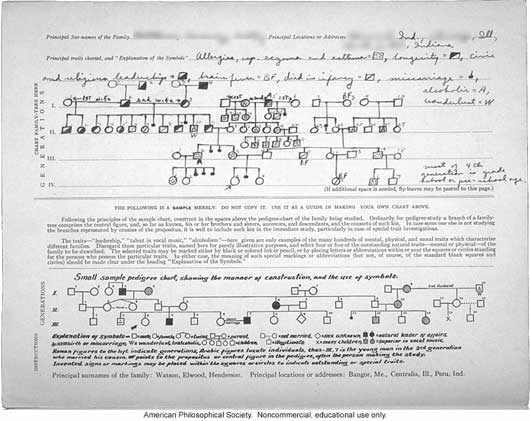
\includegraphics[width=0.75\linewidth]{images1/chart_pedigree_allergy2} 

}

\caption{Gráfico de linhagens para alergias}\label{fig:figA14}
\end{figure}

\hfill\break

\begin{figure}

{\centering 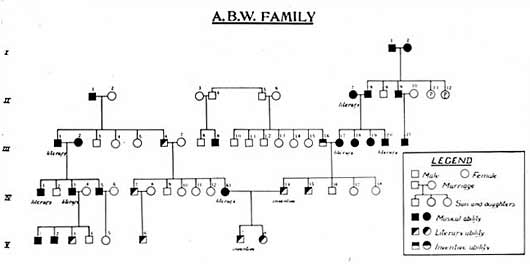
\includegraphics[width=0.75\linewidth]{images1/chart_pedigree_music2 (1)} 

}

\caption{Gráfico de linhagens para aptidão musical}\label{fig:figA15}
\end{figure}

\hfill\break

\begin{figure}

{\centering 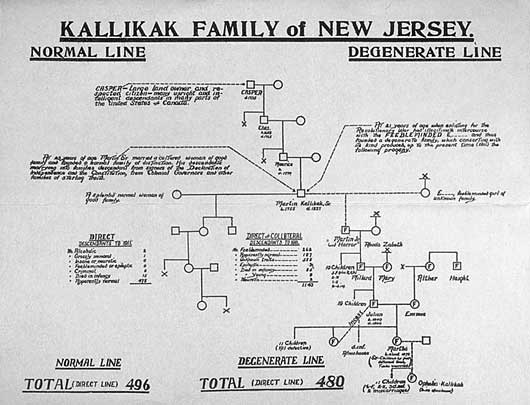
\includegraphics[width=0.75\linewidth]{images1/chart_Kallikak_pedigree2} 

}

\caption{Linhas "normais" e "degeneradas" da família Kallikak (New Jersey)}\label{fig:figA16}
\end{figure}

\hfill\break

\begin{figure}

{\centering 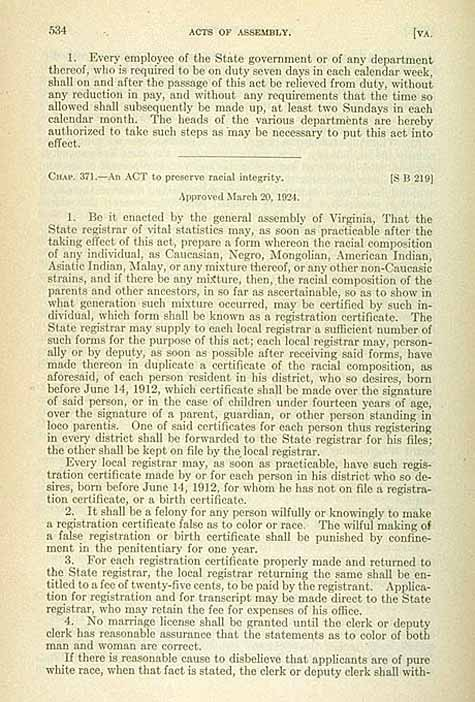
\includegraphics[width=0.75\linewidth]{images1/VA_racial_integrity_act2} 

}

\caption{Lei da Inegridade Racia (Virginia, EUA, 1924)}\label{fig:figA17}
\end{figure}

\hfill\break

\begin{figure}

{\centering 
\includegraphics[width=0.75\linewidth]{images1/choosing_love_over_eugenics} 

}

\caption{Licença para casamento}\label{fig:figA18}
\end{figure}

\hypertarget{introduuxe7uxe3o-conceitual-essencial}{%
\chapter{Introdução conceitual essencial}\label{introduuxe7uxe3o-conceitual-essencial}}

\hfill\break

\begin{quote}
``Estatística é a ciência de coletar, organizar, apresentar, analisar e interpretar dados{[}\ldots{]}'' (Ronald A. Fisher)
\end{quote}

\hfill\break

De modo geral, a estatística pode ser dividida em três grandes áreas:

\begin{itemize}
\tightlist
\item
  descritiva;
\item
  probabilidade; e,
\item
  inferencial.
\end{itemize}

\hfill\break

\hypertarget{estatuxedstica-descritiva}{%
\section{Estatística descritiva}\label{estatuxedstica-descritiva}}

Nos primeiros trabalhos estatísticos, os dados coletados eram inicialmente apresentados na forma de tabelas e gráficos.

A \textbf{estatística descritiva} se ocupa de tudo o que seja relacionado a dados: coleta, processamento, descrição (seja na forma tabular ou gráfica) e sínteses numéricas (de locação, de dispersão, de repartição) sem inferir coisa alguma além da informação trazida pelos dados. Vem experimentando crescente uso em todas as áreas científicas e desenvolvimento:

\begin{itemize}
\tightlist
\item
  crescente uso de uma abordagem quantitativa em todas as ciências;
\item
  disponibilidade de recursos computacionais;
\item
  quantidade de dados coletados.
\end{itemize}

A palavra \textbf{estatística} pode assumir diferentes significados:

\begin{itemize}
\tightlist
\item
  no singular: \textbf{estatística} \vspace{0.5cm}

  \begin{itemize}
  \tightlist
  \item
    refere-se à ciência que compreende métodos que são usados na coleta, análise, interpretação e apresentação de dados quantitativos ou qualitativos (numéricos ou não); e,
  \item
    denota uma medida ou fórmula específica (tais como uma média, um intervalo de valores, uma taxa de crescimento, um índice).
  \end{itemize}
\item
  no plural: \textbf{estatísticas}

  \begin{itemize}
  \tightlist
  \item
    refere-se a dados coletados de maneira sistemática com um propósito específico definido em qualquer campo de estudo (nesse sentido, as \emph{estatísticas} também podem ser consideradas como agregados de fatos expressos em forma numérica).
  \end{itemize}
\end{itemize}

\hypertarget{estatuxedstica-inferencial}{%
\section{Estatística inferencial}\label{estatuxedstica-inferencial}}

A \textbf{estatística inferencial} tem o objetivo de estabelecer níveis de confiança da tomada de decisão de associar uma estimativa amostral a um parâmetro populacional. Divide-se em estimação e testes de significância.

\begin{quote}
``Dedução e indução são procedimentos racionais que nos levam do já conhecido ao ainda não conhecido; isto é, permitem que adquiramos conhecimentos novos graças a conhecimentos já adquiridos.{[}\ldots{]}''
\end{quote}

Dedução.

Na dedução parte-se de uma verdade já conhecida para demonstrar que ela se aplica a todos os casos particulares iguais. Vai do geral ao particular.

Indução.

Na indução parte-se de alguns casos particulares iguais ou semelhantes para se estipular uma \textbf{lei geral}. Vai do particular ao geral.

Na dedução, dado \textbf{X}, infiro (concluo) \textbf{a}, \textbf{b}, \textbf{c}, \textbf{d}.

Na indução, dados \textbf{a}, \textbf{b}, \textbf{c}, \textbf{d}, infiro (concluo) \textbf{X}.

\begin{quote}
Exemplo: testes de aceleração (0-60 mph) feitos com 6 carros importados em 1999 resultaram nas seguintes medidas: 12,9 s; 16,50 s; 11,30 s; 15,20 s; 18,20 s e 17,70 s. Um estudo descritivo poderia afirmar que:
\end{quote}

\begin{itemize}
\tightlist
\item
  metade dos dados coletados acelera de 0-60 mph em menos de 16,00 s; e
\item
  a aceleração média de 0-60 mph é de 15,30 s.
\end{itemize}

\begin{quote}
Mas, a partir dessa amostra concluir que a aceleração média de \textbf{todos} os carros importados em 1999 seja de 15,30 s; ou, que \textbf{metade} dos carros importados em 1999 acelerem de 0-60 mph em menos de 16,00 s são afirmações que pertencem à \textbf{inferência estatística}.
\end{quote}

\hypertarget{produuxe7uxe3o-de-conhecimento}{%
\section{Produção de conhecimento}\label{produuxe7uxe3o-de-conhecimento}}

\begin{quote}
``A ciência não consegue provar coisa alguma. Ela pode apenas refutar as coisas {[}\ldots{]}'' (Karl Popper)
\end{quote}

\hfill\break

\begin{figure}

{\centering 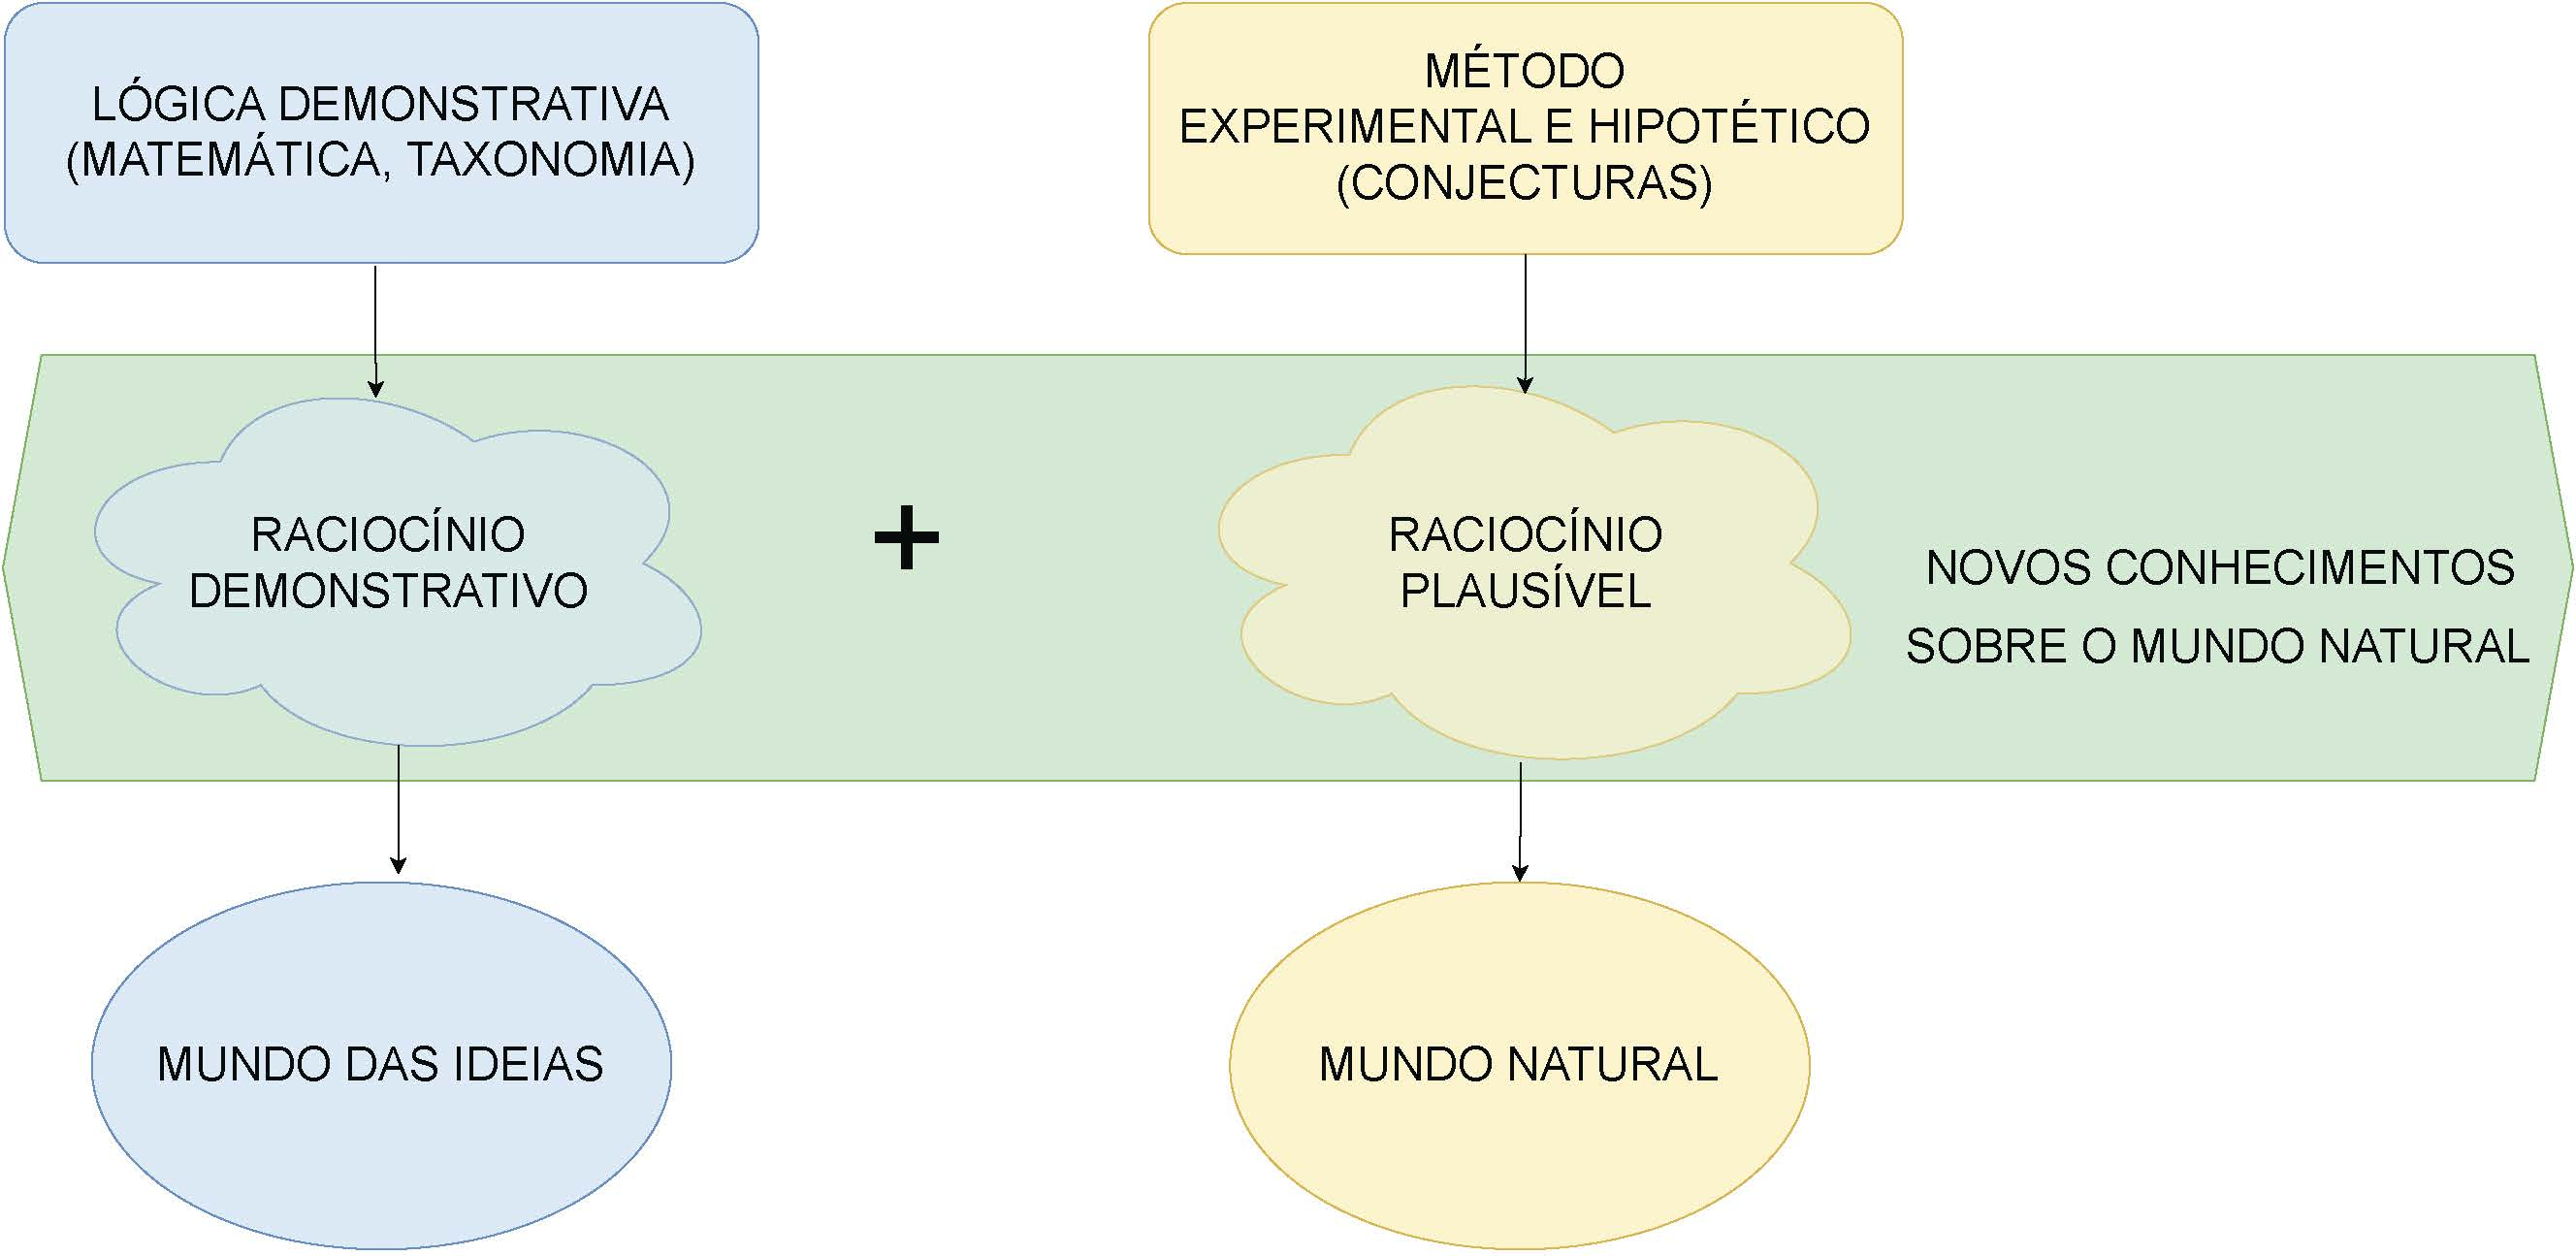
\includegraphics[width=1\linewidth]{images2/polya} 

}

\caption{Método demonstrativo e Método experimental hipotético (George Polya, 1954)}\label{fig:unnamed-chunk-4}
\end{figure}

\hfill\break

Na expansão de qualquer área do conhecimento propomos hipóteses que serão avaliadas mediante a coleta de dados que, depois de analisados, revelarão informações que, eventualmente, nos conduzirão ao afastamento da hipótese original e à proposição de outras, num processo contínuo.

\hfill\break

\begin{figure}

{\centering 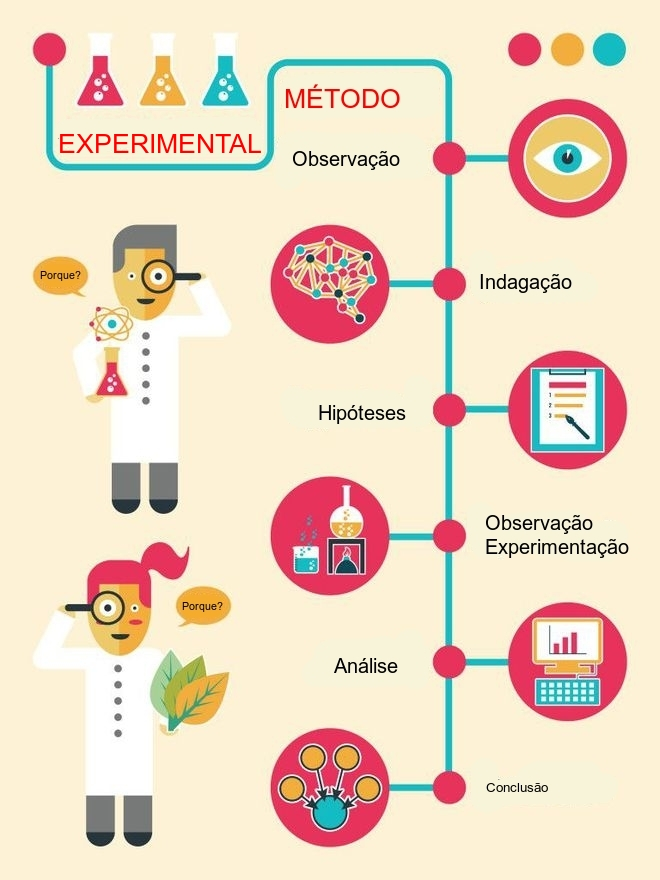
\includegraphics[width=0.6\linewidth]{images2/metodo_experimental} 

}

\caption{Método experimental hipotético}\label{fig:unnamed-chunk-5}
\end{figure}

\hfill\break

Uma investigação científica deve envolver, em linhas gerais:

\hfill\break

\begin{itemize}
\tightlist
\item
  observação dos fatos;
\item
  descrição das características essenciais, segundo o que se obteve através da observação;
\item
  explicação dessas características descritivas;
\item
  previsão; e,
\item
  decisão pertinente à investigação.
\end{itemize}

\hfill\break

O planejamento de uma pesquisa deve envolver, em linhas gerais:

\hfill\break

\begin{itemize}
\tightlist
\item
  definição do \emph{universo}: é necessário delimitar claramente, no tempo e espaço, o âmbito do inquérito, definindo, em termos precisos, o \emph{universo} a ser trabalhado;
\item
  exame das informações disponíveis: deve-se reunir todo o material existente: mapas, artigos, livros, relatórios relativos a levantamentos semelhantes;
\item
  tipos de levantamentos: completo ou amostral;
\item
  prazo;
\item
  custo;
\item
  precisão.
\end{itemize}

\hypertarget{populauxe7uxe3o-universo-amostra}{%
\section{População (universo) \& amostra}\label{populauxe7uxe3o-universo-amostra}}

\begin{figure}

{\centering 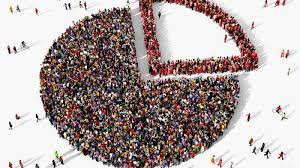
\includegraphics[width=1\linewidth]{images2/amostragem} 

}

\caption{Universo e amostra}\label{fig:unnamed-chunk-6}
\end{figure}

Quase que, invariavelmente, em todo ramo de conhecimento, o pesquisador esbarra em uma séria de limitações das mais variadas ordens (econômica, técnica, ética, geográfica, temporal,\ldots) que impossibilitam o estudo dos dados e informações associados a todos os casos existentes (\textbf{população ou universo}).

Por essa razão, através de um procedimento estatístico denominado de amostragem, estuda-se uma população (universo) a partir de uma amostra. Amostra é, portanto, um subconjunto finito e representativo da população (universo), extraído de modo sistemático (planejado).

\hypertarget{paruxe2metros-e-estatuxedsticas}{%
\section{Parâmetros e estatísticas}\label{paruxe2metros-e-estatuxedsticas}}

É comum a adoção de letras gregas para as características descritivas que se referirem à poúlação (universo) e letras do alfabeto latino para aquelas relativas à amostra extraída:

\begin{longtable}[]{@{}lll@{}}
\toprule\noalign{}
Característica estudada & Notação populacional & Notação amostral \\
\midrule\noalign{}
\endhead
\bottomrule\noalign{}
\endlastfoot
Número de elementos & N & n \\
Média & \(\mu\) & \(\stackrel{-}{x}\) \\
Variância & \(\sigma^{2}\) & \({s}^{2}\) \\
Desvio padrão & \(\sigma\) & s \\
Proporção & \(\Pi\) & p \\
\end{longtable}

\begin{figure}

{\centering 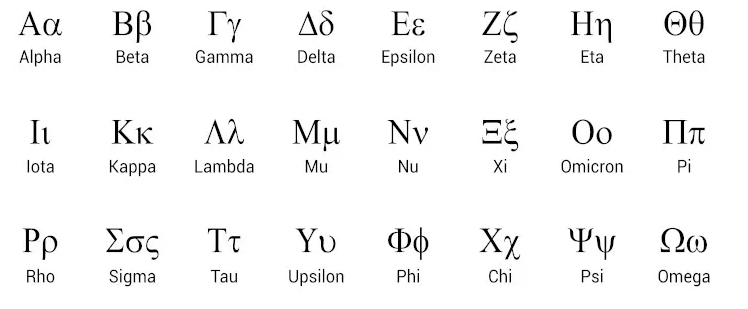
\includegraphics[width=1\linewidth]{images2/alf_grego} 

}

\caption{Alfabeto grego}\label{fig:unnamed-chunk-7}
\end{figure}

\hypertarget{tipos-de-variuxe1veis}{%
\section{Tipos de variáveis}\label{tipos-de-variuxe1veis}}

Variáveis quantitativas

\begin{itemize}
\tightlist
\item
  contínuas: são os dados com maior potencial de produzir informação significativa dentre todos: comprimentos, áreas, pesos, densidades; e,
\item
  discretas: são dados com um pouco menos de informação que os de natureza contínua mas possuem mais informação que dados qualitativos: número de andares de um prédio, de degraus de uma escada, número de filhos de um casal.
\end{itemize}

Variáveis qualitativas

\begin{itemize}
\tightlist
\item
  ordinais: apresentam um pouco mais de informação que os dados qualitativos puramente nominais na medida que suas classes podem ser interpretadas como possuindo um ordenamento inerente: padrão construtivo (baixo, médio, alto), classe econômica de rendimento (baixa, média, alta), nível de escolaridade (fundamental, médio e superior); e,
\item
  nominais: são dados a menor quantidade de informação: sexo, cor, códigos postais de cidades;
\end{itemize}

Codificação de variáveis qualitativas

\begin{itemize}
\tightlist
\item
  binárias: pela associação de valores numéricos: 0 ou 1 a uma variável qualitativa nominal que se apresente com apenas dois aspectos: sim ou não, ausência ou presença. Pela composição de mais variáveis binárias pode-se codificar variáveis que possuam um número maior de classes; e,
\item
  \emph{proxy}: pela associação de valores numéricos contínuos que guardam ``correlação'\,' com as classes da variável qualitativa nominal.
\end{itemize}

\begin{figure}

{\centering 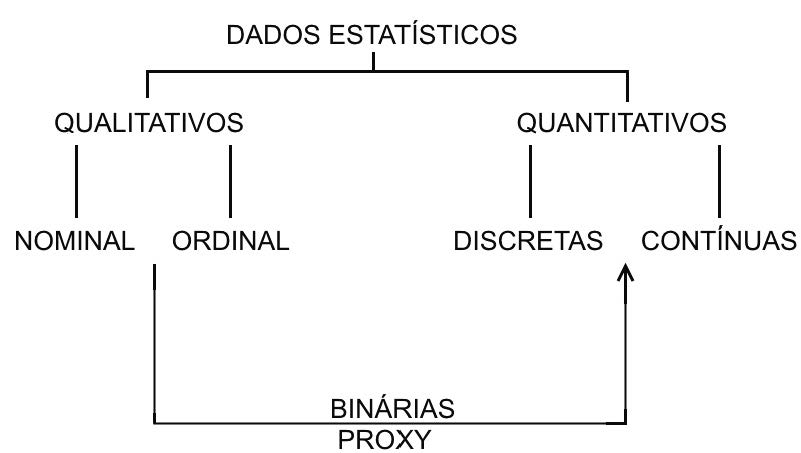
\includegraphics[width=0.75\linewidth]{images2/tipos_variaveis} 

}

\caption{Tipos e codificações de variáveis }\label{fig:unnamed-chunk-8}
\end{figure}

\hypertarget{indexauxe7uxe3o-de-dados-i}{%
\section{\texorpdfstring{Indexação de dados (\(i\))}{Indexação de dados (i)}}\label{indexauxe7uxe3o-de-dados-i}}

Muitas operações matemáticas são representadas trazendo os valores dos dados indicados de modo genérico por letras (gregas ou romanas) e índices como, por exemplo, \(x_{i}\). Tal notação está a indicar que, se dispuséssemos os dados em uma linha virtual (às vezes necessitando que estejam ordenados, como para a determinação de uma separatiz), cada um de seus valores estaria a ocupar uma \emph{posição} indicada pelo índice \emph{i}:

\hfill\break

\begin{figure}

{\centering 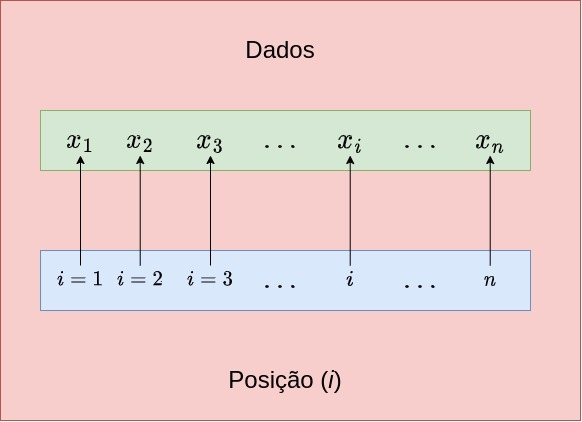
\includegraphics[width=0.6\linewidth]{images2/vetor_posicao} 

}

\caption{Entendendo a indexação de dados}\label{fig:unnamed-chunk-9}
\end{figure}

\hypertarget{nouxe7uxf5es-buxe1sicas-sobre-somatuxf3rios-sigma}{%
\section{\texorpdfstring{Noções básicas sobre somatórios (\(\Sigma\))}{Noções básicas sobre somatórios (\textbackslash Sigma)}}\label{nouxe7uxf5es-buxe1sicas-sobre-somatuxf3rios-sigma}}

Somatório é um operador matemático utilizado para simplificar expressões que envolvam soma de mais de um elemento.

Digamos, por exemplo, que estamos interessados saber o total de comissões a pagar em um determinado setor de uma empresa.

Admita que esse setor tenha 6 funcionários: Pedro, Guilherme, Lucas, Maria, Fernanda e Roberto e que suas comissões sejam R\$ 3000; R\$ 3300; R\$ 3900; R\$ 2950; R\$ 3150 e R\$ 3450.

A representação da soma das comissões pode ser expressa de vários modos como, por exemplo, nesse extensa frase:

\hfill\break

\begin{quote}
O total de comissões a pagar em um determinado setor de uma empresa é a Renda do Pedro mais a Renda do Guilherme mais a Renda do Lucas mais a Renda da Maria mais a Renda da Fernanda mais Renda do Roberto.
\end{quote}

\hfill\break

Atribuindo os valores para cada uma das rendas:

\hfill\break

\begin{quote}
O total de comissões a pagar em um determinado setor de uma empresa é: : R\$ 3000 + R\$ 3300 + R\$ 3900 + R\$ 2950 + R\$ 3150 + R\$ 3450.
\end{quote}

\hfill\break

Chamando-se ``O total de comissões a pagar em um determinado setor de uma empresa é'' de \(X\), teremos:

\hfill\break

\begin{quote}
\(X\) = R\$ 3000 + R\$ 3300 + R\$ 3900 + R\$ 2950 + R\$ 3150 + R\$ 3450.
\end{quote}

\hfill\break

Para simplificar a representação dessa operação, vamos enumerar os funcionários: Pedro (1), Guilherme (2), Lucas (3), Maria (4), Fernanda (5) e Roberto (6). Além disso, vamos chamar a comissão a ser paga pela letra X.

Para diferenciar a fração da comissão \(X\) a ser paga a cada um dos funcionários podemos por um índice na letra \(X\) para indicar a quem estamos nos referindo. Assim \(X_{1}\) seria a comissão do Pedro, \(X_{2}\) a do Guilherme, \(X_{3}\) a do Lucas, \(X_{4}\) a da Maria, \(X_{5}\) a da Fernanda e \(X_{3}\) a do Roberto.

Com essa notação podemos representar matematicamente o total das comissões a pagar em um determinado setor de uma empresa por:

\begin{quote}
\(X=X_{1}+X_{2}+X_{3}+X_{4}+X_{5}+X_{6}\)
\end{quote}

Cada um desses fatores pode ser generalizado como um \(X_{i}\), a comissão de um \emph{i-ésimo} funcionário qualquer. Sabendo que o setor tem apenas 6 funcionários (Pedro, Guilherme, Lucas, Maria, Fernanda e Roberto) então esse i irá variar de 1 a 6 (Pedro:1, Guilherme: 2, Lucas: 3, Maria: 4, Fernanda: 5 e Roberto: 6).

Com todas essas considerações podemos representar a soma das comissões utilizando a notação matemática do somatório.

A letra grega maiúscula \textbf{\(\Sigma\) (sigma)} é habitualmente adotada na matemática para representar o somatório de uma quantidade de fatores. Assim, nosso exemplo da soma de 6 fatores (comissões) pode ser representada matematicamente por:

\[
\sum_{i=1}^{6}{X_{i}} = X_{1}+X_{2}+X_{3}+X_{4}+X_{5}+X_{6}
\]

Observe que abaixo da letra \(\Sigma\) vemos \(i=1\) indicando que o índice dos fatores (X) a serem somados (a \emph{i-ésima} comissão) irá se iniciar pela comissão do primeiro funcionário, quando então i = 1.

Acima da letra \(\Sigma\) vemos o número \(6\) indicando que o índice dos fatores (X) a serem somados irá se dar até o valor da comissão do sexto funcionário, quando então i=6.

Generalizando-se para uma soma de \(n\) fatores \(X\):

\[
\sum_{i=1}^n{X_{i}}.
\]

A representação matemática do somatório pode ser inserida junto a qualquer outra operação como, por exemplo, podemos, depois de realizar a soma, dividi-la por um valor \(n\) qualquer

\[
\frac{\sum_{i=1}^n{X_{i}}}{n} \\
\]

ou elevá-la ao quadrado:

\[
\left(\sum_{i=1}^n{X_{i}}\right)^{2}
\]

Atenção para a diferença entre essas duas operações:

\[
\left(\sum_{i=1}^n{X_{i}}\right)^{2}  
\]
e

\[
\sum_{i=1}^n{X_{i}^{2}}
\]

A primeira indica que devemos realizar a soma dos fatores \textbf{e só então elevar esse resultado ao quadrado}. A segunda indica que devemos realizar a \textbf{soma dos quadrados de cada um dos fatores}.

\hypertarget{anuxe1lise-combinatuxf3ria-diagramas-de-uxe1rvore-permutauxe7uxf5es-arranjos-combinauxe7uxf5es}{%
\section{Análise combinatória: diagramas de árvore, permutações (arranjos) \& combinações}\label{anuxe1lise-combinatuxf3ria-diagramas-de-uxe1rvore-permutauxe7uxf5es-arranjos-combinauxe7uxf5es}}

\hfill\break

A análise combinatória é um conjunto de técnicas para agrupamento de objetos conforme regras definidas e obtenção, através de cálculos, do número de agrupamentos possíveis.

\hfill\break

Se um evento \(E\) pode ser decomposto em eventos sequenciais \(E_{1}\), \(E_{2}\), \(E_{2}\), \ldots, \(E_{n}\) e existem \(P_{1}\) possibilidades distintas de ocorrer \(E_{1}\), \(P_{2}\) possibilidades distintas de ocorrer \(E_{2}\) e assim sucessivamente, então o número total de possibilidades do evento \(E\) ocorrer é dado por:

\hfill\break

\[
P_{1}.P_{2}. \hspace{0.5cm}... \hspace{0.5cm}.P_{n}
\]\\

Esse princípio recebe o nome de \emph{Princípio multiplicativo}, e é aplicado nos casos em que os eventos são interligados pelo conectivo \textbf{e}, característico de decisões sucessivas.

\hfill\break

Se um homem tem 2 camisas e 4 gravatas, então ele tem \(2 \times 4 = 8\) formas de combinar uma camisa com uma gravata.

\hfill\break

Um diagrama como ilustrado na Figura \ref{fig:fig12} (denominado \textbf{diagrama de árvore} em virtude de sua aparência) geralmente é usado para explicar o princípio acima

\hfill\break

\begin{figure}

{\centering 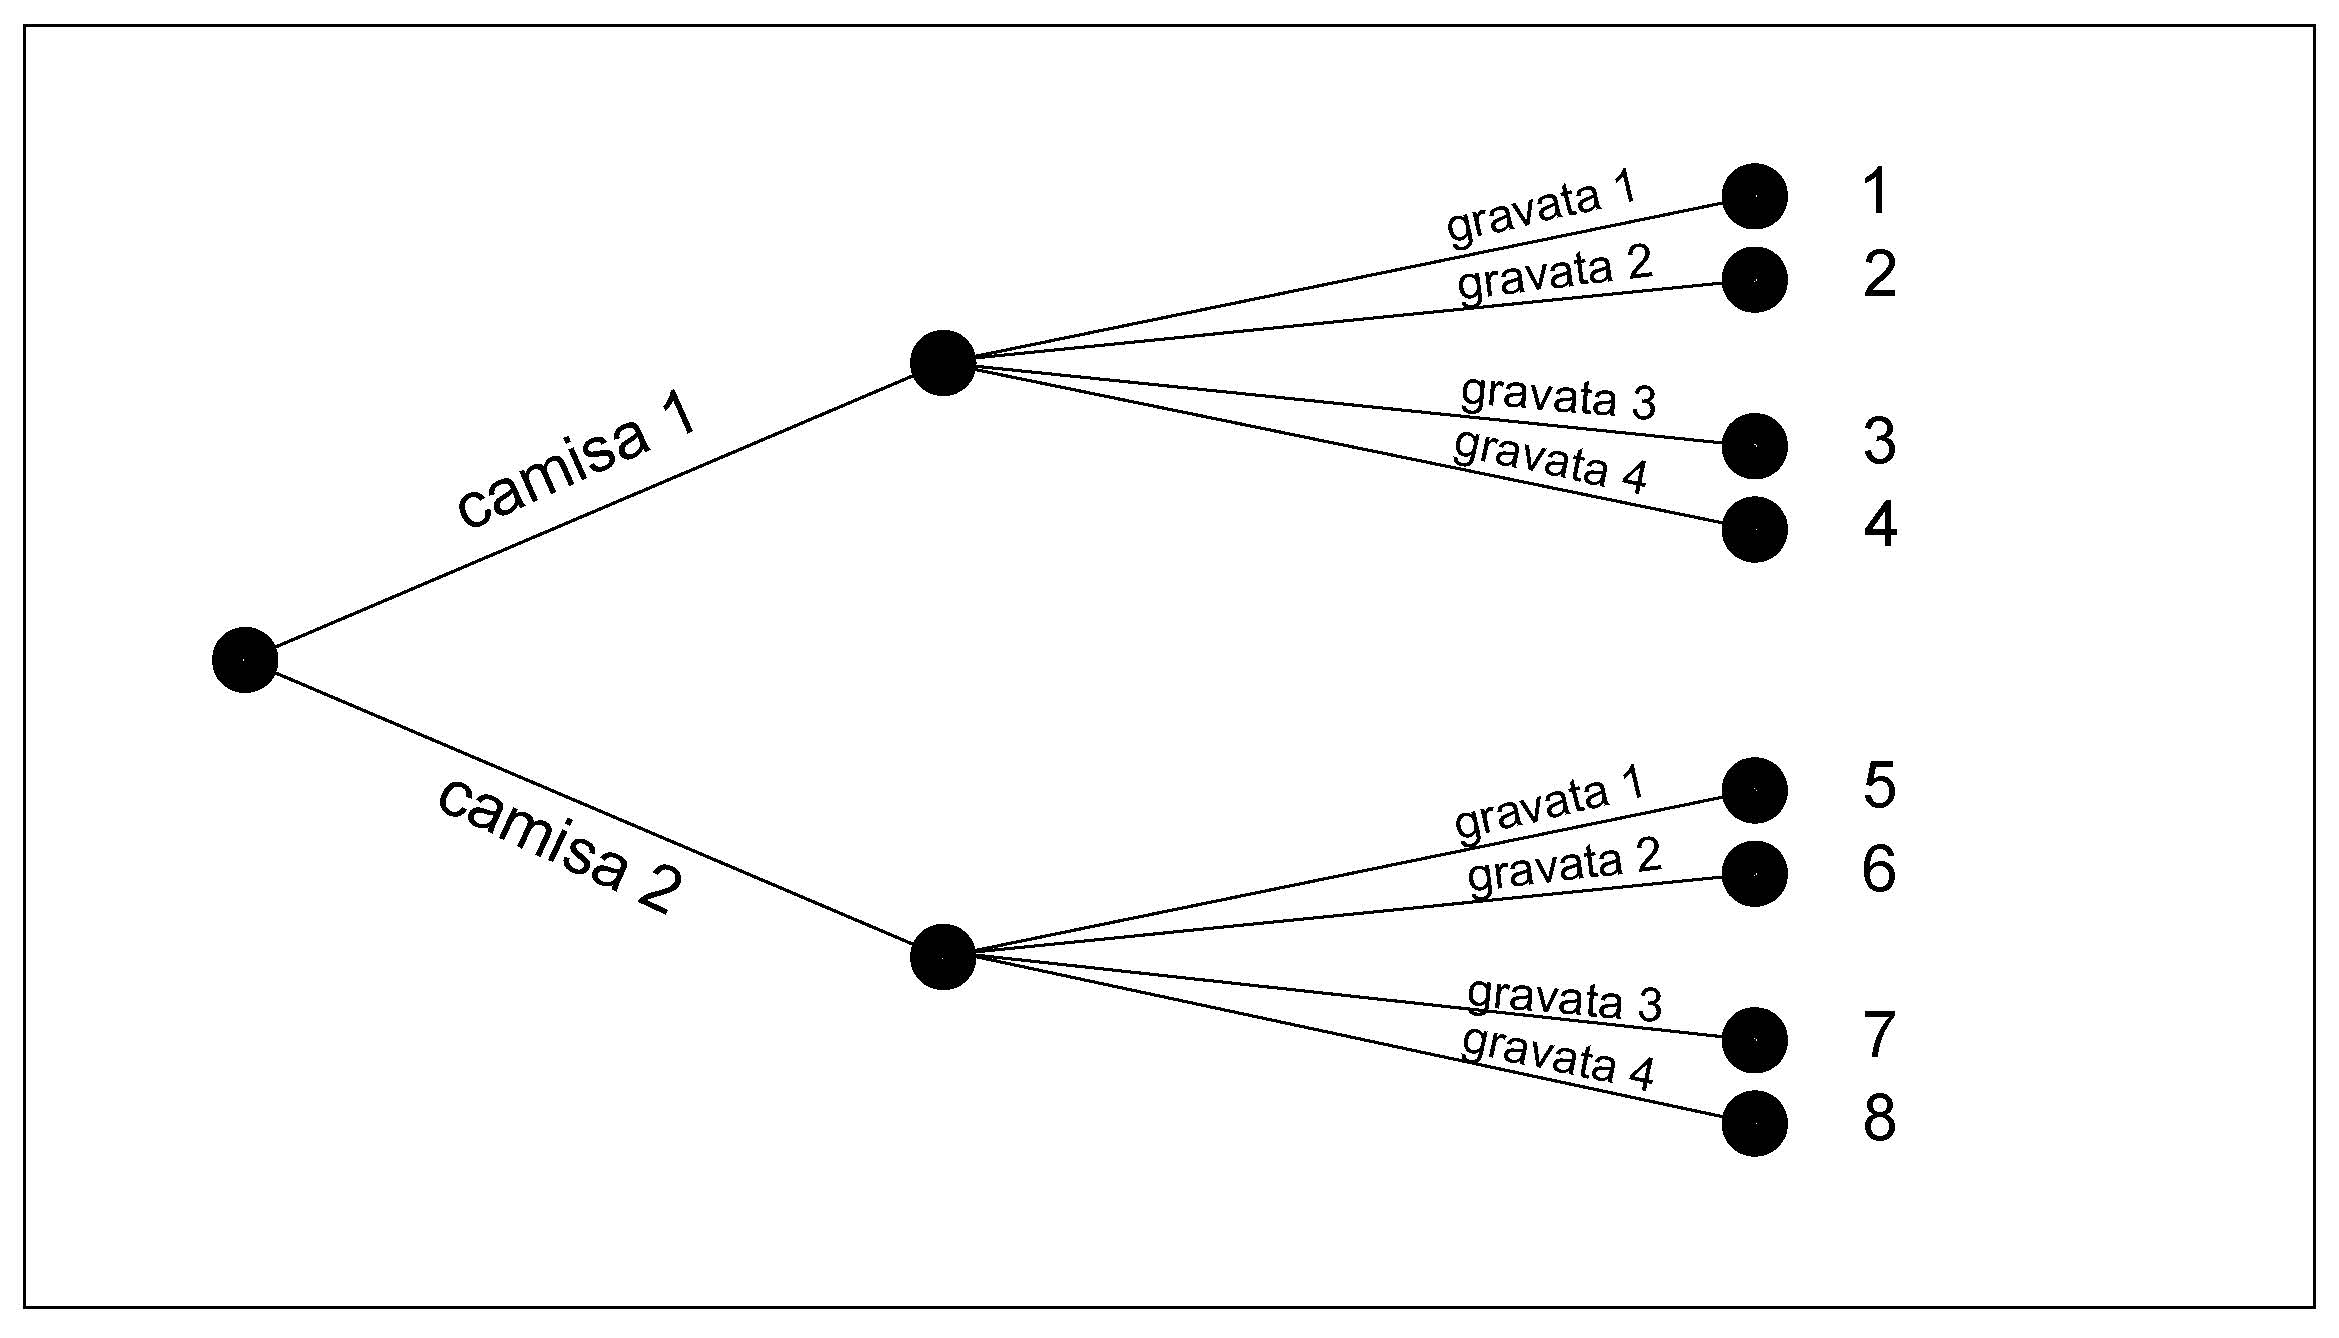
\includegraphics[width=0.5\linewidth]{images4/diagrama_arvore} 

}

\caption{Diagrama de árvore}\label{fig:fig12}
\end{figure}

\hfill\break

Ao lançarmos uma moeda três vezes (assumindo-se que K: cara e C: coroa) haverá \(2 \times 2 \times 2 = 8\) possibilidades distintas.

\hfill\break

O \textbf{diagrama de árvore} associado será (cf.~Figura \ref{fig:fig13}:

\hfill\break

\begin{figure}

{\centering 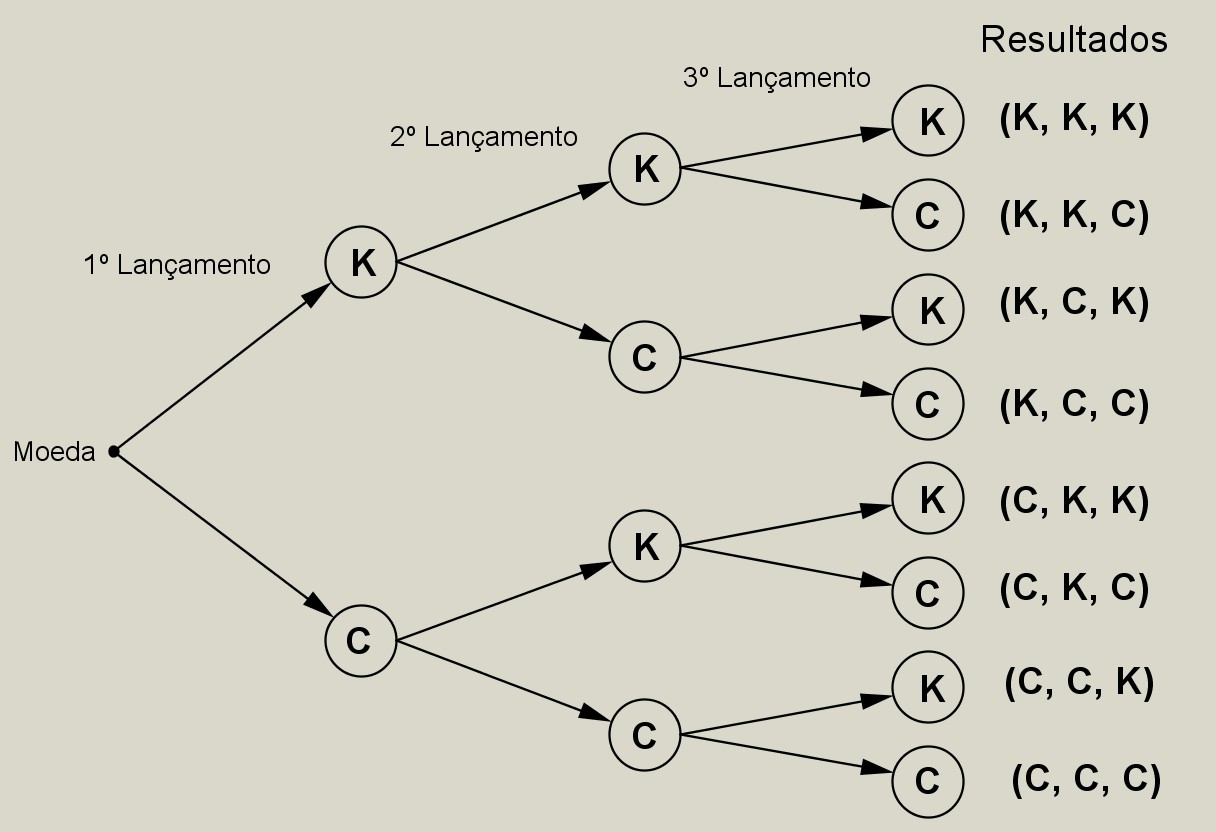
\includegraphics[width=0.5\linewidth]{images4/diagrama_arvore_moeda} 

}

\caption{Diagrama de árvore}\label{fig:fig13}
\end{figure}

\hfill\break

Sejam os eventos mutuamente exclusivos \(E_{1}\) com \(n{1}\) possibilidades distintas de ocorrer, \(E_{2}\) com \(n_{2}\), \ldots, \(E_{n}\) com \(n_{k}\); então o número total de possibilidades de ocorrer \textbf{pelo menos um desses eventos} será dado por:

\[
n_{2} + n_{2} + ... + n_{k}
\]

\hfill\break

Esse princípio recebe o nome de \emph{Princípio aditivo}, e é aplicado nos casos em que os eventos são interligados pelo conectivo \textbf{ou}, característico de eventos mutuamente exclusivos.

\hfill\break

Uma cantina de um colégio possui três tipos de sucos e dois tipos de refrigerantes. Um aluno pode adquirir apenas 1 suco ou 1 refrigerante. Quantas possibilidades de escolha ele tem?

\hfill\break

Seja \(E_{1}\) definido como escolher um tipo de suco (\(n_{1}=3\)) e \(E_{2}\) definido como escolher 1 tipo de refrigerante (\(n_{2}=2\). Então o número total de possíveis escolhas será dado aplicando-se o princípio aditivo:

\hfill\break

\[
n_{1} + n_{2}=5
\]

\hfill\break

\hypertarget{permutauxe7uxf5es-ou-arranjos}{%
\subsection{Permutações ou arranjos}\label{permutauxe7uxf5es-ou-arranjos}}

~

O conceito de uma permutação (arranjo) refere-se a uma relação de \(n\) objetos distintos que serão agrupados \(p\) ~\(p\) (\(p < n\)). Nos agrupamentos possíveis considera-se a ordem dos elementos; sendo assim, qualquer mudança na ordem dos elementos em um agrupamento constitui um novo agrupamento: \textbf{agrupamentos que possuem os mesmos objetos em ordem distinta são considerados agrupamentos distintos}.

\hfill\break

\begin{itemize}
\tightlist
\item
  Simples: não ocorre a repetição de um elemento no agrupamento; e,\\
\item
  Com repetição: os elementos que compõem o conjunto podem aparecer repetidos; ou seja, um agrupamento pode apresentar elementos iguais.
\end{itemize}

\hfill\break

O número de permutações (arranjos) \textbf{sem a repetição} de um mesmo elemento no agrupamento, formados por \(p\) elementos selecionados de um conjunto de \emph{n} objetos distintos será:

\[
P_{(n,p)} =  \frac{n!}{(n-p)!}
\]

\hfill\break

\begin{quote}
Exemplo: Quantos agrupamentos diferentes (onde a ordem dos elementos é razão para distinção: \emph{permutações}) formados por \textbf{3 letras cada} podem ser formados com as \textbf{7 letras}: A, B, C, D, E, F, G \textbf{sem repetição}?
\end{quote}

\hfill\break

\begin{align*}
n  & = 7 \\
p  & = 3 \\
P_{(n,p)} & = \frac{7!}{ (7-3)!} \\
          & = \frac{7!}{4!} = \\
          & = \frac{ 7 \times 6 \times 5 \times 4! }{4!}  \\
          & = 7 \times 6 \times 5  = 210   
\end{align*}

\hfill\break

O número de permutações (arranjos) \textbf{com repetição} de um mesmo elemento no agrupamento, formados por \(p\) elementos selecionados de um conjunto de \(n\) objetos distintos será:

\[
P_{(n,p)} =  n ^{p}
\]

\hfill\break

\begin{quote}
Exemplo: Quantos agrupamentos diferentes (onde a ordem dos elementos é razão para distinção: \textbf{permutações}) formados por \textbf{3 letras cada} podem ser formados com as \textbf{7 letras}: A, B, C, D, E, F, G \textbf{com repetição}?
\end{quote}

\hfill\break

\begin{align*}
n   &  = 7 \\
p   &  = 3 \\
P_{(n,p)} &  = n^{p} \\
          &   = 7 ^{3} = 343
\end{align*}

\hfill\break

\hypertarget{combinauxe7uxf5es}{%
\subsection{Combinações}\label{combinauxe7uxf5es}}

Em uma \emph{permutação} consideramos que a \textbf{ordem* que os objetos assumem nos agrupamentos os tornam diferentes uns dos outros. Por exemplo, }abc** é uma agrupamento distinto de \textbf{bca} numa permutação.

\hfill\break

Em muitos problemas, entretanto, estamos interessados somente na seleção ou escolha dos objetos **sem que a ordem assumida pelos objetos nos agrupamentos os tornem diferentes uns dos outros*.

\hfill\break

Tais seleções são chamadas de \emph{combinações}. Por exemplo, \textbf{abc} e \textbf{bca} são consideradas uma mesma combinação.

\hfill\break

O conceito de uma combinação refere-se a uma relação de \(n\) objetos distintos que serão agrupados \(p\) a \(p\) (\(p < n\)) sem repetição de qualquer objeto em um mesmo agrupamento. Os agrupamentos que possuem os mesmos objetos em ordem diferente \textbf{não são considerados agrupamentos distintos}.

\hfill\break

\begin{itemize}
\tightlist
\item
  Simples: não ocorre a repetição de elementos no agrupamento; e,\\
\item
  Com repetição: os elementos que compõem o agrupamento podem aparecer repetidos; ou seja, ocorre a repetição de um mesmo elemento em um agrupamento.
\end{itemize}

\hfill\break

O número total de combinações sem repetição, de \(p\) objetos selecionados de \(n\) (também chamado de combinações de \(n\) elementos tomados \(p\) a cada vez) é representado por:

\hfill\break
\[
C_{(n,p)} = \frac{ n! }{ p! \times ( n-p)!} 
\]

\hfill\break

\begin{quote}
Exemplo: Qual é número de formas nas quais \(3\) cartas podem ser escolhidas ou selecionadas de um total de \(8\) cartas diferentes?
\end{quote}

\hfill\break

\begin{align*}
n & = 8 \\
p & = 3 \\
C_{(n,p)} & = \frac{8!}{ 3! (8-3)!}  \\
          & = \frac{8!}{3! \times 5!} \\
          & = \frac{ 8 \times 7 \times 6 \times 5! }{ 3! \times 5! } \\
          & = \frac{ 8 \times 7 \times 6 }{3!} = 56  
\end{align*}

\hfill\break

O número total de combinações com repetição, de \(p\) objetos selecionados de \(n\) (também chamado de combinações de \(n\) elementos tomados \(p\) a cada vez com repetição) é representado por:

\hfill\break

\[
C_{(n+p-1,p)} = \frac{ (n+p-1)! }{ p! \times ( n-1)!}
\]

\hfill\break

\begin{quote}
Exemplo: Supondo que você queira comprar um sorvete com 4 bolas em uma sorveteria que possui 3 sabores disponíveis: chocolate, baunilha e morango. De quantos modos diferentes você pode fazer esta compra? (Note que nesta combinação é possível repetir a ordem de dois ou mais sabores, assim tratando de uma combinação com repetição).
\end{quote}

\hfill\break

\begin{align*}
n & =  3 \\
p & = 4 \\ 
C_{(n+p-1,p)} & = \frac{(3+4-1)!}{ 4! (+3-1)!} = 15  
\end{align*}

\hfill\break

\hypertarget{observauxe7uxf5es-acerca-de-alguns-fatoriais}{%
\subsection{Observações acerca de alguns fatoriais}\label{observauxe7uxf5es-acerca-de-alguns-fatoriais}}

~

\begin{align*}
P_{(n,n)} & = \frac{n!}{(n-n)!} = \frac{n!}{0!} = n! \\
C_{(n,0)} & = \frac{n!}{ 0! \times (n-0)! } = \frac{n!}{ 1 \times (n)!} = 1 \\
C_{(n,1)} & = \frac{n! }{ 1! (n-1)!} \\
   & = \frac{ n! }{(n-1)! } \\
   & = \frac{ n \times (n-1)! }{ (n-1)!} = n    
\end{align*}

\hypertarget{conectivos-luxf3gicos}{%
\section{Conectivos lógicos}\label{conectivos-luxf3gicos}}

Muitos dos problemas ligados à probabilidade de ocorrência de eventos são propostos com o auxílio de conectivos lógicos:

\hfill\break

\begin{itemize}
\tightlist
\item
  \textbf{Proposição}: a afirmação de que algo é verdadeiro. Após analisarmos qualquer proposição, podemos defini-la como verdadeira ou falsa como, por exemplo: ``o céu é azul'';
\item
  \textbf{Negação}: negação do valor lógico de uma proposição. A negação de uma proposição verdadeira é falsa. A negação de uma proposição falsa é verdadeira. Os símbolos da negação são o til \(^{-}\) ou \(^{c}\);
\item
  \textbf{Conjunção}: proposição composta com a utilização do conectivo ``e'' como, por exemplo: ``o céu é azul e as nuvens são brancas''. Os símbolos usuais para uma conjunção são: \(\cap\) ou a letra ``V'' invertida; e,
\item
  \textbf{Disjunção}: proposição composta com a utilização do conectivo ``ou'' como, por exemplo, ``o céu é azul ou os pássaros são pretos''. Os símbolos usuais para uma disjunção são: \(\cup\) ou a letra \(V\).
\end{itemize}

\hypertarget{leis-de-de-morgan}{%
\section{Leis de De Morgan}\label{leis-de-de-morgan}}

Augustus de Morgan foi um matemático e lógico indiano.

\hfill\break

\begin{figure}

{\centering 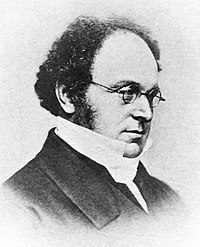
\includegraphics[width=0.5\linewidth]{images4/de_morgan} 

}

\caption{Augustus De Morgan (1806 - 1871)}\label{fig:unnamed-chunk-10}
\end{figure}

\hfill\break

Primeira Lei de De Morgan:

\hfill\break

Negar duas proposições ligadas com ``e'' (\(\cap\)); ou seja, uma \textbf{conjunção}, é o mesmo que negar duas proposições e ligá-las com ``ou''' (ou seja, transformá-las em uma disjunção). Considerando as proposições ``p'' e ``q'' teremos:

\hfill\break

\begin{itemize}
\tightlist
\item
  \(\sim (p \cap q) = (~p) \cup (~q)\); ou,\\
\item
  \((p \cap q)^{c} = (p^{c}) \cup (q^{c})\).
\end{itemize}

\hfill\break

Segunda Lei de De Morgan:

\hfill\break

Negar duas proposições ligadas por ``ou''' (\(\cup\)); ou seja, uma \textbf{disjunção}, é o mesmo que negar as duas proposições e ligá-las com ``e'' (ou seja, transformá-las em uma conjunção). Considerando as proposições ``p'' e ``q'' teremos:

\hfill\break

\begin{itemize}
\tightlist
\item
  \(\sim (p \cup q) = (~p) \cap (~q)\); ou,\\
\item
  \((p \cup q)^{c}= (p^{c}) \cap (q^{c})\).
\end{itemize}

\hypertarget{nouxe7uxf5es-buxe1sicas-para-o-uso-de-calculadora-cassio-fx-82ms}{%
\section{Noções básicas para o uso de calculadora (Cassio fx-82MS)}\label{nouxe7uxf5es-buxe1sicas-para-o-uso-de-calculadora-cassio-fx-82ms}}

Em estatística trabalha-se muito com a análise de um ou mais conjuntos de dados, sendo comum a realização de diversas operações matemáticas com esses dados. Muitas dessas operações envolvem somatórios, por exemplo, e para simplificar essas operações o uso da calculadora se torna essencial.

Neste curso recomenda-se o uso de uma calculadora científica. Existem diversas calculadoras que cumprem as funções necessárias nesse curso. Para padronizar as aulas, alguns professores sugerem a calculadora científica de código: FX82MS, que é a calculadora que cujo funcionamento será exibido a seguir, passo a passo. A seguir serão descritas algumas das funções básicas mais importantes no uso desta calculadora.

Primeiro vamos deixar a calculadora no modo de regressão linear. Esse modo permite que a calculadora
funcione normalmente para as operações comuns (soma, subtração, multiplicação e divisão), e ainda libera
todas as funções importantes nesse curso. Sempre que o aluno for utilizar a calculadora, ele deve se certificar que ela esteja no modo de regressão linear, da seguinte forma:

PASSO 1:

\begin{itemize}
\item
  \begin{enumerate}
  \def\labelenumi{\arabic{enumi}.}
  \tightlist
  \item
    ON
  \end{enumerate}
\item
  \begin{enumerate}
  \def\labelenumi{\arabic{enumi}.}
  \setcounter{enumi}{1}
  \tightlist
  \item
    MODE
  \end{enumerate}
\item
  \begin{enumerate}
  \def\labelenumi{\arabic{enumi}.}
  \setcounter{enumi}{2}
  \tightlist
  \item
    Aperte 3 para escolher REG
  \end{enumerate}
\item
  \begin{enumerate}
  \def\labelenumi{\arabic{enumi}.}
  \setcounter{enumi}{3}
  \tightlist
  \item
    Aperte 1 para escolher LIN
  \end{enumerate}
\end{itemize}

Repare que no topo do visor da calculadora apareceu o símbolo \textcolor{red}{REG}, que indica que a calculadora está em modo de regressão. Desde que esteja no modo de regressão, podemos passar para o passo seguinte.

O nosso objetivo aqui é inserir o conjunto de dados na calculadora para então realizarmos as operações necessárias. Mas antes de inserir os dados, temos que garantir que a calculadora esteja \textcolor{red}{vazia} para o novo conjunto de dados. Ou seja, devemos limpar a calculadora:

PASSO 2:

\begin{itemize}
\item
  \begin{enumerate}
  \def\labelenumi{\arabic{enumi}.}
  \tightlist
  \item
    SHIFT
  \end{enumerate}
\item
  \begin{enumerate}
  \def\labelenumi{\arabic{enumi}.}
  \setcounter{enumi}{1}
  \tightlist
  \item
    MODE
  \end{enumerate}
\item
  \begin{enumerate}
  \def\labelenumi{\arabic{enumi}.}
  \setcounter{enumi}{2}
  \tightlist
  \item
    Aperte 1 para escolher Scl ( \emph{Stat Clear})
  \end{enumerate}
\item
  \begin{enumerate}
  \def\labelenumi{\arabic{enumi}.}
  \setcounter{enumi}{3}
  \tightlist
  \item
    Aperte = para limpar a calculadora
  \end{enumerate}
\end{itemize}

Entrada de dados.

Agora que a calculadora está em modo de regressão e está limpa, podemos inserir o conjunto de dados. Para ilustrar esta função, vamos inserir o seguinte conjunto de dados: \(X= {5,3,6,2}\).

Para inserir cada um desses elementos você deve digitar o número e em seguida o botão M+.

A sequência fica assim: 5 M+ 3 M+ 6 M+ 2 M+.

A cada vez que você insere uma observação, a calculadora atualiza o número de observações inseridas. No final, nesse caso, aparece \textcolor{red}{n=4} porque inserimos 4 observações.

Funções envolvendo somatórios.

Observe na calculadora os botões \textcolor{orange}{shift} e \textcolor{red}{alpha}. Geralmente estes botões aparecem nas cores amarela e vermelha, respectivamente. Observe ainda que alguns botões da calculadora possuem termos nessas cores. Para selecionar as funções em \textcolor{orange}{amarelo}, antes devemos ligar o modo \textcolor{orange}{shift}. Enquanto que para selecionar as funções em \textcolor{red}{vermelho} deve-se ligar o modo \textcolor{red}{alpha}.

Por exemplo, para abrir a função \textcolor{orange}{S-SUM} que está em \textcolor{orange}{amarelo} no botão 1, faz-se: SHIFT 1. A função \textcolor{orange}{S-SUM} é a que contém todos os somatórios importantes. Ao abrir esta função aparecem três opções da seguinte forma:

\[
\Sigma(x) \\
\Sigma(x^{2})\\
n 
\]

Aperta-se 1 = para ter o somatório de \(x\); 2 = para ter o somatório de \(x^{2}\) ou 3 = para saber o número \(n\) de obervações inseridas.

Funções para obter a média e o desvio padrão.

A função \textcolor{orange}{S-VAR} fornece a média e o desvio padrão dos dados. Essas são medidas importantes, que serão utilizadas durante todo o curso. Para abrir esta função faz-se: SHIFT 2.

\[
\stackrel{-}{x}
\sigma_{x}
S_{x}
\]

A opção 1 retorna a média dos dados, a opção 2 retorna o desvio padrão populacional e a opção 3 o desvio padrão amostral.

Como inserir dois conjuntos de dados.

Quando se deseja estudar dois conjuntos de dados, de mesmo tamanho, pode-se inseri-los de forma simultânea na calculadora. Para ilustrar vamos inserir os seguintes conjuntos de dados: \(X={2,7,4,3,2}\) e \(Y={1,2,3,6,5}\). \textcolor{red}{Antes de inserir os dados, lembre-se de limpar a calculadora}.

Em seguida vamos inserir os dados de 2 em 2: o primeiro de X com o primeiro de Y e assim por diante. Repare que ao lado do botão M+ tem um botão com uma vírgula. Esta vírgula é utilizada para separar as observações de X das de Y . A sequência fica assim:

\begin{itemize}
\tightlist
\item
  2,1 M+
\item
  7,2 M+
\item
  4,3 M+
\item
  3,6 M+
\item
  2,5 M+
\end{itemize}

Se você usar a função \textcolor{orange}{S-SUM}, na tela vai aparecer os somatórios apenas de X, que foi pela ordem, o primeiro a ser inserido. Na calculadora tem um botão grande e style=``color:gray;''\textgreater S-SUM, com 4 setas. Depois de selecionar a função \textcolor{orange}{amarelo} aperte a seta para frente que aparecerão os somatórios para Y . O mesmo acontece para a função \textcolor{orange}{S-VAR}.

\begin{figure}

{\centering 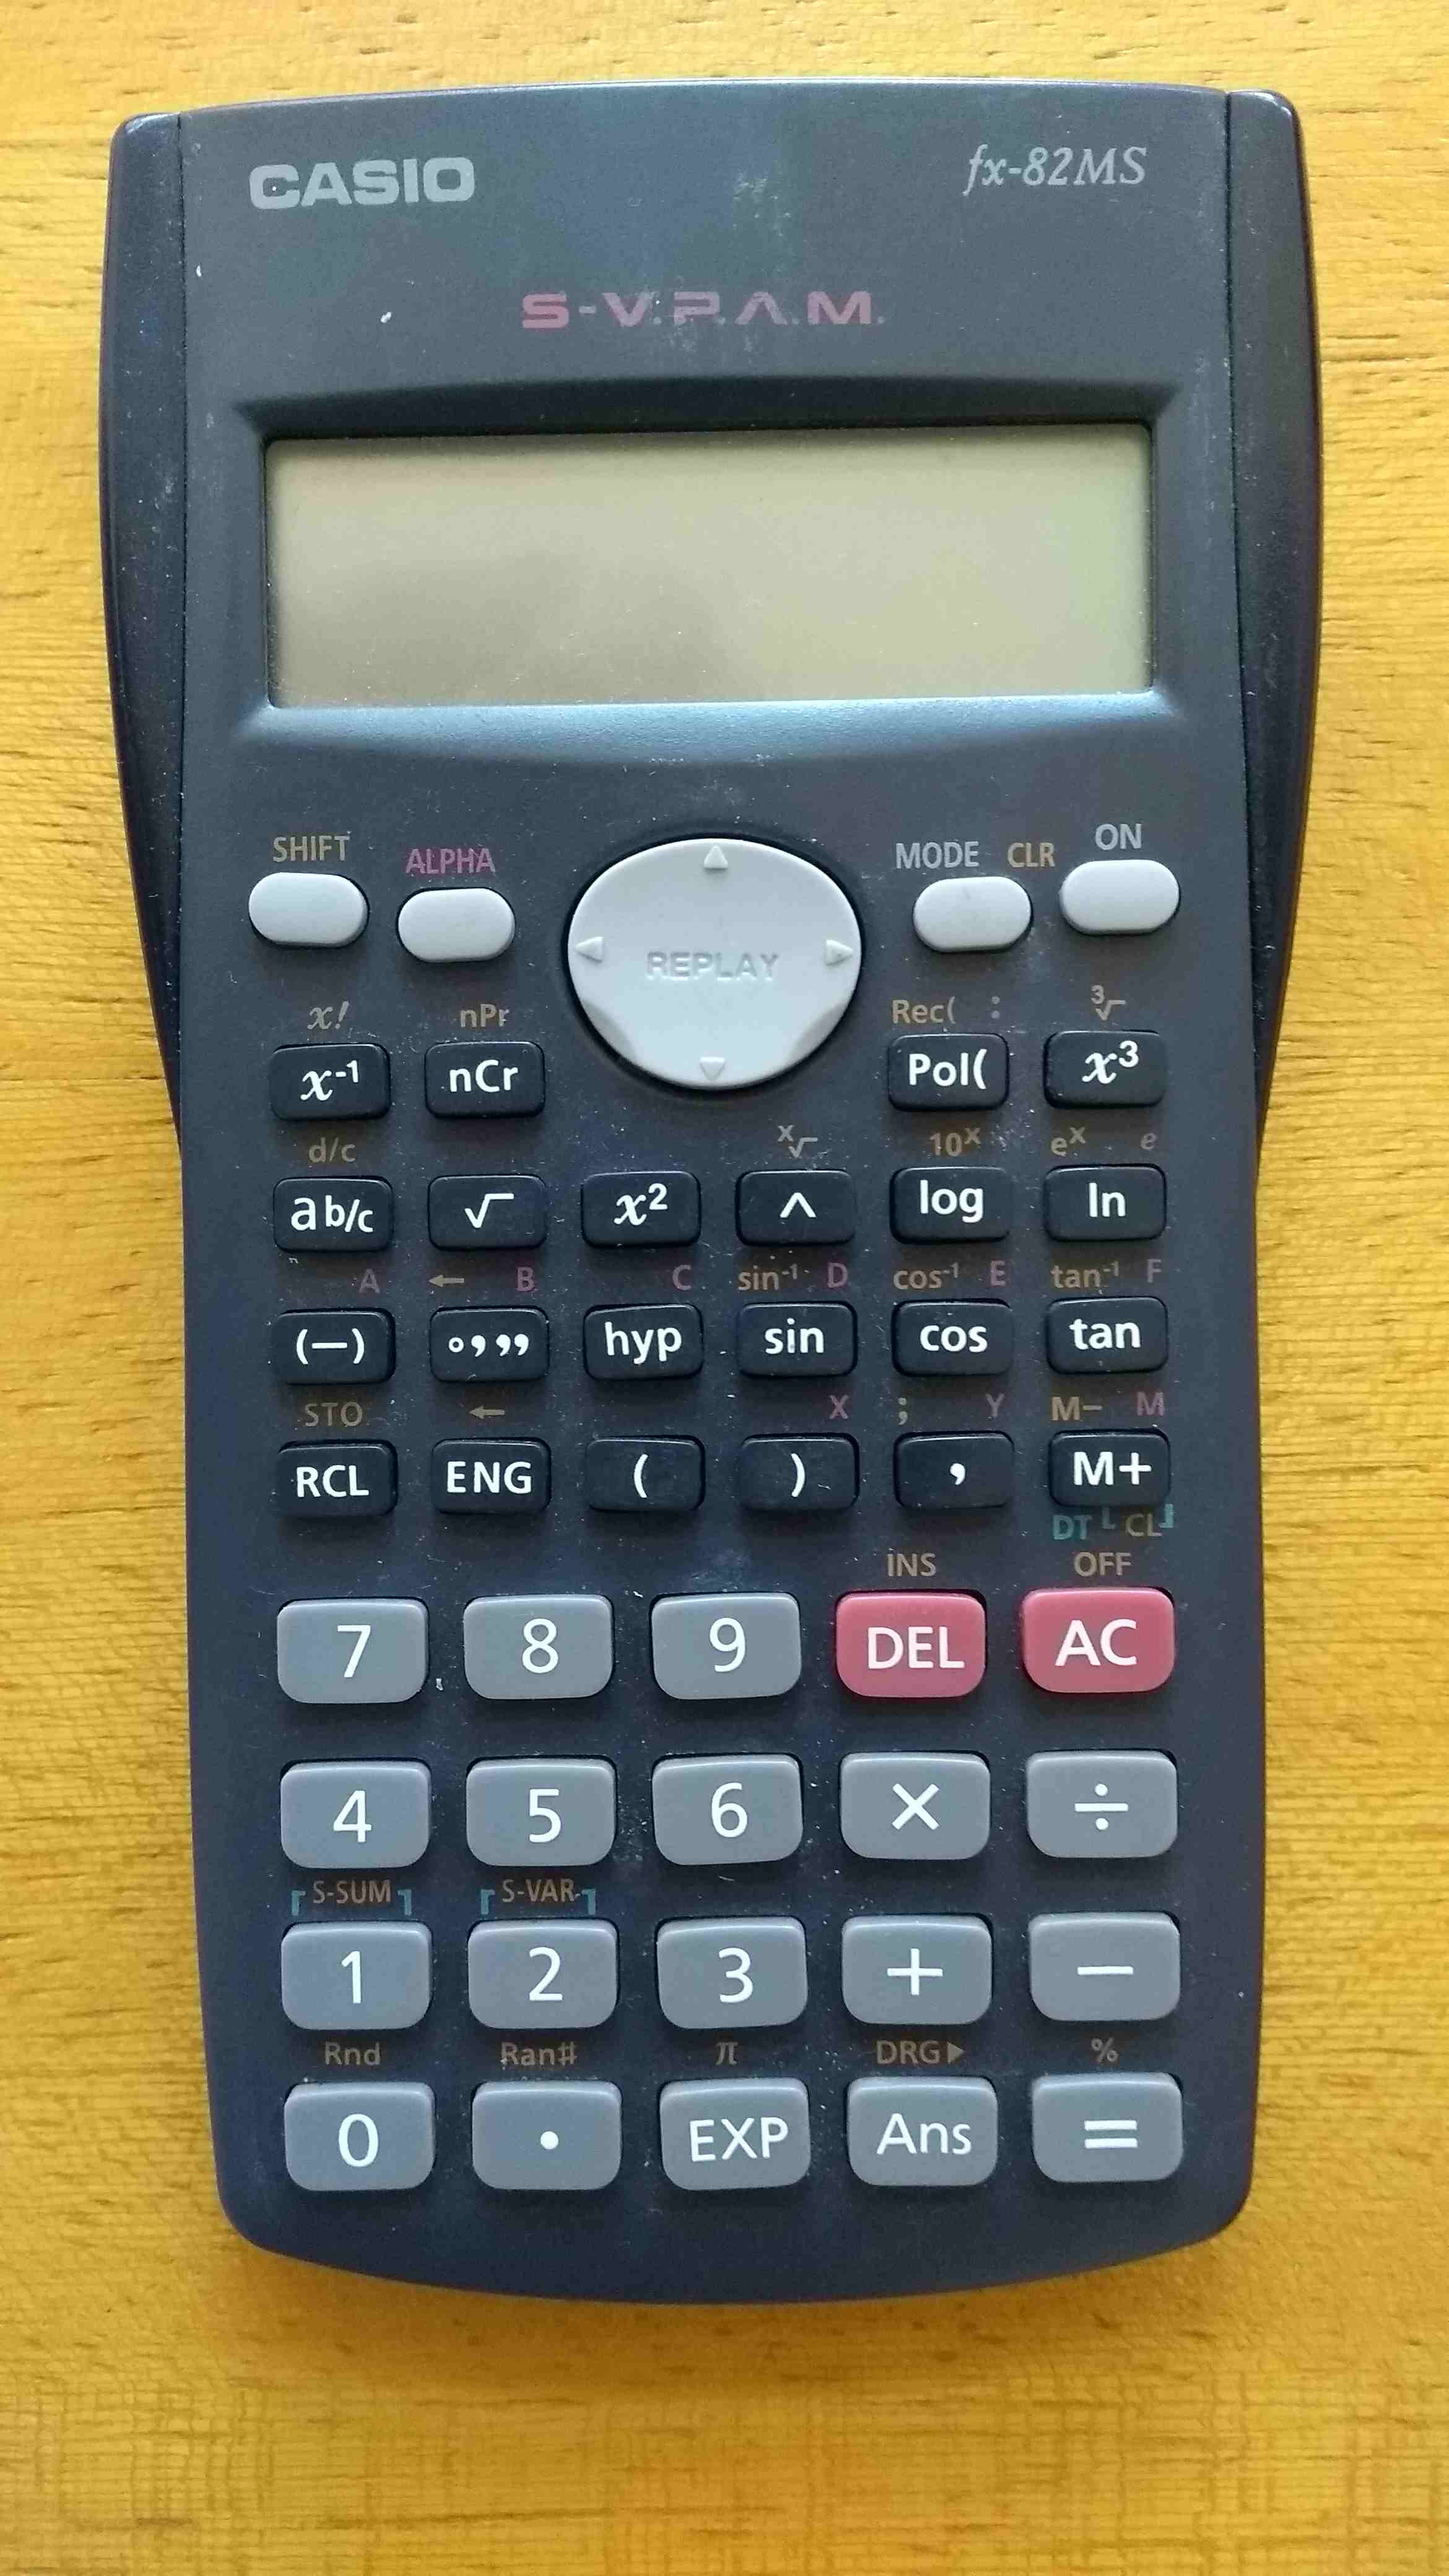
\includegraphics[width=0.8\linewidth]{images2/calculadora_cassio} 

}

\caption{Calculadora Cassio}\label{fig:unnamed-chunk-11}
\end{figure}

\hypertarget{introduuxe7uxe3o-uxe0-estatuxedstica-descritiva}{%
\chapter{Introdução à estatística descritiva}\label{introduuxe7uxe3o-uxe0-estatuxedstica-descritiva}}

\hfill\break

Sobre o estudo da estatística por áreas nas quais, aparentemente, não se vislumbra sua utilidade trazemos o prefácio da tradução do livro de Jack Levin (Estatística aplicada às ciências humanas) por Sérgio Francisco Costa, ao dizer que o livro:

\hfill\break

\begin{quote}
``{[}\ldots{]} destina-se a um público muito específico: estudantes de Ciências Humanas, refúgio errôneo dos que fogem das equações e dos cálculos, pois que, embora humanas - e talvez por isso mesmo - não podemos prescindir das tão odiadas quantificações {[}\ldots{]}''
\end{quote}

\hfill\break

\hypertarget{anuxe1lise-exploratuxf3ria}{%
\section{Análise exploratória}\label{anuxe1lise-exploratuxf3ria}}

\hfill\break

A análise exploratória de dados ( \emph{EDA: Exploratory Data Analisys} , originalmente desenvolvida pelo matemático e estatístico norte-americano John Tukey na década de 1970) é usada para se investigar conjuntos de dados e resumir suas principais características, muitas vezes usando métodos de visualização de dados por gráficos e apresentação de tabelas.

\hfill\break

\begin{figure}

{\centering 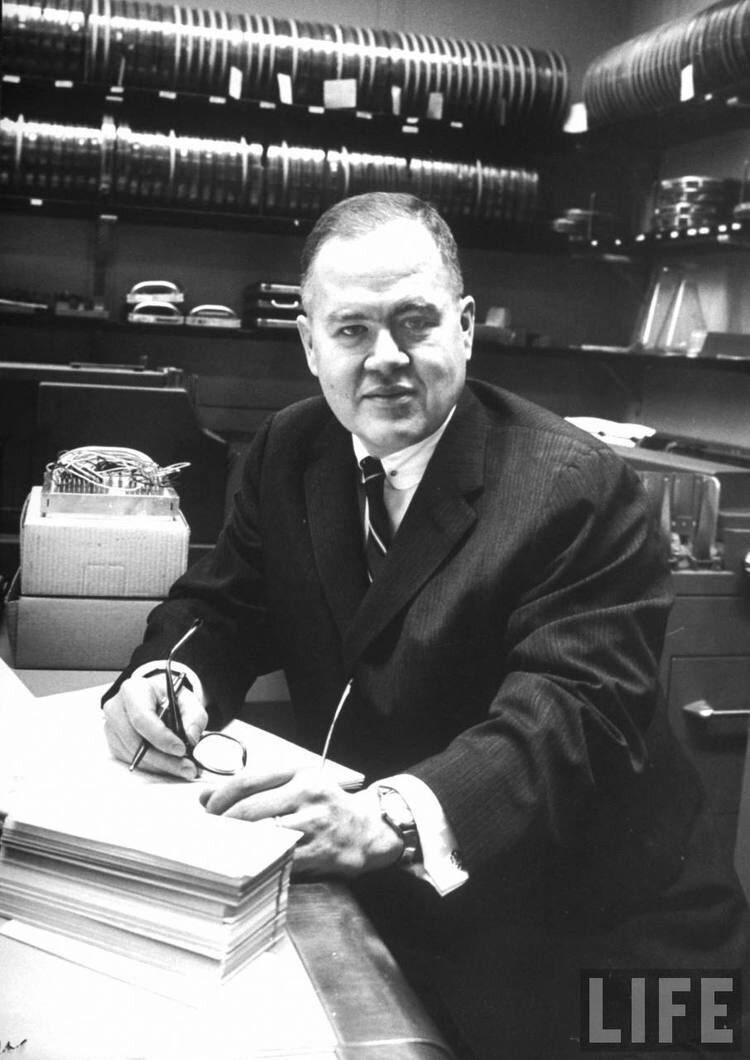
\includegraphics[width=0.5\linewidth]{images3/tukey} 

}

\caption{John Tukey (1915-2000)}\label{fig:unnamed-chunk-14}
\end{figure}

\hfill\break

Habitualmente uma \emph{EDA} envolve:

\begin{itemize}
\tightlist
\item
  verificar quais são os tipos de variáveis presentes nos dados;
\item
  sintetizar os valores assumidos por cada uma das variáveis;
\item
  verificar os padrões de cada variável e eventuais associações entre duas ou mais delas; e,
\item
  apresentação de tabelas e gráficos expositivos variados.
\end{itemize}

\hypertarget{dados-brutos-em-rol-diagrama-de-ramos-folhas-e-de-dispersuxe3o-unidimensional}{%
\section{Dados brutos, em rol, diagrama de ramos \& folhas e de dispersão unidimensional}\label{dados-brutos-em-rol-diagrama-de-ramos-folhas-e-de-dispersuxe3o-unidimensional}}

Consideremos os dados obtidos da medição das alturas em metros de 60 estudantes de uma determinada classe de um certo curso aqui na UEL:

\begin{Shaded}
\begin{Highlighting}[]
\NormalTok{alturas}\OtherTok{=}\FunctionTok{c}\NormalTok{(}\FloatTok{1.63}\NormalTok{,}\FloatTok{1.67}\NormalTok{,}\FloatTok{1.47}\NormalTok{,}\FloatTok{1.64}\NormalTok{,}\FloatTok{1.66}\NormalTok{,}\FloatTok{1.73}\NormalTok{,}\FloatTok{2.00}\NormalTok{,}\FloatTok{1.62}\NormalTok{,}\FloatTok{1.65}\NormalTok{,}\FloatTok{1.56}\NormalTok{,}\FloatTok{1.65}\NormalTok{,}\FloatTok{1.85}\NormalTok{,}\FloatTok{1.73}\NormalTok{,}
          \FloatTok{1.78}\NormalTok{,}\FloatTok{1.82}\NormalTok{,}\FloatTok{1.68}\NormalTok{,}\FloatTok{1.67}\NormalTok{,}\FloatTok{1.83}\NormalTok{,}\FloatTok{1.72}\NormalTok{,}\FloatTok{1.71}\NormalTok{,}\FloatTok{1.73}\NormalTok{,}\FloatTok{1.67}\NormalTok{,}\FloatTok{1.66}\NormalTok{,}\FloatTok{1.95}\NormalTok{,}\FloatTok{1.76}\NormalTok{,}\FloatTok{1.73}\NormalTok{,}
          \FloatTok{1.77}\NormalTok{,}\FloatTok{1.68}\NormalTok{,}\FloatTok{1.65}\NormalTok{,}\FloatTok{1.64}\NormalTok{,}\FloatTok{1.66}\NormalTok{,}\FloatTok{1.68}\NormalTok{,}\FloatTok{1.61}\NormalTok{,}\FloatTok{1.73}\NormalTok{,}\FloatTok{1.72}\NormalTok{,}\FloatTok{1.83}\NormalTok{,}\FloatTok{1.69}\NormalTok{,}\FloatTok{1.84}\NormalTok{,}\FloatTok{1.66}\NormalTok{,}
          \FloatTok{1.78}\NormalTok{,}\FloatTok{1.54}\NormalTok{,}\FloatTok{1.74}\NormalTok{,}\FloatTok{1.56}\NormalTok{,}\FloatTok{1.66}\NormalTok{,}\FloatTok{1.56}\NormalTok{,}\FloatTok{1.62}\NormalTok{,}\FloatTok{1.55}\NormalTok{,}\FloatTok{1.86}\NormalTok{,}\FloatTok{1.44}\NormalTok{,}\FloatTok{1.67}\NormalTok{,}\FloatTok{1.76}\NormalTok{,}\FloatTok{1.79}\NormalTok{,}
          \FloatTok{1.75}\NormalTok{,}\FloatTok{1.41}\NormalTok{,}\FloatTok{1.65}\NormalTok{,}\FloatTok{1.58}\NormalTok{,}\FloatTok{1.93}\NormalTok{,}\FloatTok{1.57}\NormalTok{,}\FloatTok{1.71}\NormalTok{,}\FloatTok{1.58}\NormalTok{,}\FloatTok{0.1}\NormalTok{,}\FloatTok{3.68}\NormalTok{,}\DecValTok{0}\NormalTok{,}\ConstantTok{NA}\NormalTok{)}
\NormalTok{alturas}
\end{Highlighting}
\end{Shaded}

\begin{verbatim}
##  [1] 1.63 1.67 1.47 1.64 1.66 1.73 2.00 1.62 1.65 1.56 1.65 1.85 1.73 1.78 1.82
## [16] 1.68 1.67 1.83 1.72 1.71 1.73 1.67 1.66 1.95 1.76 1.73 1.77 1.68 1.65 1.64
## [31] 1.66 1.68 1.61 1.73 1.72 1.83 1.69 1.84 1.66 1.78 1.54 1.74 1.56 1.66 1.56
## [46] 1.62 1.55 1.86 1.44 1.67 1.76 1.79 1.75 1.41 1.65 1.58 1.93 1.57 1.71 1.58
## [61] 0.10 3.68 0.00   NA
\end{verbatim}

\hfill\break
\emph{Garbage in}, \emph{garbage out}. Não são raras as vezes nas quais o relatório com os dados coletados em uma pesquisa apresentam uma série de erros. Não estamos a nos refeir aqui aos \textbf{erros amostrais} mas sim aos erros experimentais (não amostrais), aqueles decorrentes de dados coletados incorretamente, tais como aqueles resultantes de omissões na transcrição das informações, da leitura de instrumentos descalibrados ou de informações simplesmente não coletadas.

\hfill\break

Denomina-se pré-processamento essa etapa de \emph{limpeza} do conjunto de dados na qual busca-se corrigir de mdo extremamente criterioso esses problemas e, para tanto, um profundo conhecimento do objeto que está sendo pesquisado é necessário de modo a não serem liminarmente eliminados dados simplesmente por destoarem da alguma tendência (para essas tituações há ferramentas estatísticas apropriadas).\\

\hfill\break

O conjunto original de dados ( \emph{dataset}) refere-se a alturas de pessoas (estudantes ) e assim, tata-se de uma variável quantitativa e contínua e como tal será analisada. As omissões de informação ``NA'' ( \emph{not available}) e as medidas transcritas com erros grosseiros (0 m; 0,10 m; 3,68 m) serão removidas.

\hfill\break

Assim, o \emph{dataset} será composto pelos dados abaixo:

\hfill\break

\begin{Shaded}
\begin{Highlighting}[]
\NormalTok{alturas}\OtherTok{=}\FunctionTok{c}\NormalTok{(}\FloatTok{1.63}\NormalTok{,}\FloatTok{1.67}\NormalTok{,}\FloatTok{1.47}\NormalTok{,}\FloatTok{1.64}\NormalTok{,}\FloatTok{1.66}\NormalTok{,}\FloatTok{1.73}\NormalTok{,}\FloatTok{2.00}\NormalTok{,}\FloatTok{1.62}\NormalTok{,}\FloatTok{1.65}\NormalTok{,}\FloatTok{1.56}\NormalTok{,}\FloatTok{1.65}\NormalTok{,}\FloatTok{1.85}\NormalTok{,}\FloatTok{1.73}\NormalTok{,}
          \FloatTok{1.78}\NormalTok{,}\FloatTok{1.82}\NormalTok{,}\FloatTok{1.68}\NormalTok{,}\FloatTok{1.67}\NormalTok{,}\FloatTok{1.83}\NormalTok{,}\FloatTok{1.72}\NormalTok{,}\FloatTok{1.71}\NormalTok{,}\FloatTok{1.73}\NormalTok{,}\FloatTok{1.67}\NormalTok{,}\FloatTok{1.66}\NormalTok{,}\FloatTok{1.95}\NormalTok{,}\FloatTok{1.76}\NormalTok{,}\FloatTok{1.73}\NormalTok{,}
          \FloatTok{1.77}\NormalTok{,}\FloatTok{1.68}\NormalTok{,}\FloatTok{1.65}\NormalTok{,}\FloatTok{1.64}\NormalTok{,}\FloatTok{1.66}\NormalTok{,}\FloatTok{1.68}\NormalTok{,}\FloatTok{1.61}\NormalTok{,}\FloatTok{1.73}\NormalTok{,}\FloatTok{1.72}\NormalTok{,}\FloatTok{1.83}\NormalTok{,}\FloatTok{1.69}\NormalTok{,}\FloatTok{1.84}\NormalTok{,}\FloatTok{1.66}\NormalTok{,}
          \FloatTok{1.78}\NormalTok{,}\FloatTok{1.54}\NormalTok{,}\FloatTok{1.74}\NormalTok{,}\FloatTok{1.56}\NormalTok{,}\FloatTok{1.66}\NormalTok{,}\FloatTok{1.56}\NormalTok{,}\FloatTok{1.62}\NormalTok{,}\FloatTok{1.55}\NormalTok{,}\FloatTok{1.86}\NormalTok{,}\FloatTok{1.44}\NormalTok{,}\FloatTok{1.67}\NormalTok{,}\FloatTok{1.76}\NormalTok{,}\FloatTok{1.79}\NormalTok{,}
          \FloatTok{1.75}\NormalTok{,}\FloatTok{1.41}\NormalTok{,}\FloatTok{1.65}\NormalTok{,}\FloatTok{1.58}\NormalTok{,}\FloatTok{1.93}\NormalTok{,}\FloatTok{1.57}\NormalTok{,}\FloatTok{1.71}\NormalTok{,}\FloatTok{1.58}\NormalTok{)}
\NormalTok{alturas}
\end{Highlighting}
\end{Shaded}

\begin{verbatim}
##  [1] 1.63 1.67 1.47 1.64 1.66 1.73 2.00 1.62 1.65 1.56 1.65 1.85 1.73 1.78 1.82
## [16] 1.68 1.67 1.83 1.72 1.71 1.73 1.67 1.66 1.95 1.76 1.73 1.77 1.68 1.65 1.64
## [31] 1.66 1.68 1.61 1.73 1.72 1.83 1.69 1.84 1.66 1.78 1.54 1.74 1.56 1.66 1.56
## [46] 1.62 1.55 1.86 1.44 1.67 1.76 1.79 1.75 1.41 1.65 1.58 1.93 1.57 1.71 1.58
\end{verbatim}

\hfill\break

Esse conjunto de dados certamente contém diversas informações acerca da altura dessas pessoas; todavia, da maneira como estão expostos, a visualização dessas informações fica bastante difícil. Esse modo de apresentação é chamado de dados \emph{brutos}.

\hfill\break

Com um pequeno refinamento, como pela simples ordenação desses dados (são medidas numéricas contínuas), algumas informações começam a se destacar:

\hfill\break

\begin{Shaded}
\begin{Highlighting}[]
\FunctionTok{sort}\NormalTok{(alturas)}
\end{Highlighting}
\end{Shaded}

\begin{verbatim}
##  [1] 1.41 1.44 1.47 1.54 1.55 1.56 1.56 1.56 1.57 1.58 1.58 1.61 1.62 1.62 1.63
## [16] 1.64 1.64 1.65 1.65 1.65 1.65 1.66 1.66 1.66 1.66 1.66 1.67 1.67 1.67 1.67
## [31] 1.68 1.68 1.68 1.69 1.71 1.71 1.72 1.72 1.73 1.73 1.73 1.73 1.73 1.74 1.75
## [46] 1.76 1.76 1.77 1.78 1.78 1.79 1.82 1.83 1.83 1.84 1.85 1.86 1.93 1.95 2.00
\end{verbatim}

\hfill\break

A interpretabilidade das informações trazidas por esses dados começa a ficar mais fácil como, por exemplo, as alturas:

\hfill\break

\begin{itemize}
\tightlist
\item
  mínima; e,
\item
  máxima dos estudantes.
\end{itemize}

\hfill\break

A uma listagem de valores ordenada (de modo crescente ou decrescente) dá-se o nome de \emph{rol}.

\hfill\break

Outra forma de apresentação desses dados é por um \emph{Diagrama de Ramos e Folhas}, uma apresentação híbrida pois ao mesmo tempo que espelha a quantidade de medidas observadas para cada altura, mantém as informações da listagem.

\hfill\break

\begin{Shaded}
\begin{Highlighting}[]
\FunctionTok{stem}\NormalTok{(alturas)}
\end{Highlighting}
\end{Shaded}

\begin{verbatim}
## 
##   The decimal point is 1 digit(s) to the left of the |
## 
##   14 | 147
##   15 | 45666788
##   16 | 12234455556666677778889
##   17 | 11223333345667889
##   18 | 233456
##   19 | 35
##   20 | 0
\end{verbatim}

\hfill\break

À esquerda do traço vertical (os ramos) são apresentadas frações das medidas das alturas (no caso, decímetros) e à direita (as folhas) são apresentadas os complementos dessas medidas (os centímetros) de tal modo que cada um dos dados da amostral original possa ter sua medida resgatada fazendo-se a leitura dos valores à esquerda com cada um deles à direita.

\hfill\break

Essa apresentação também oferece uma apreciação visual a respeito de como os valores se distribuem.

\hfill\break

Um \emph{Gráfico de dispersão unidimensional (stripchart)} expressa visualmente duas informações: a localização de cada uma das medidas e a dispersão dos dados.

\hfill\break

\begin{Shaded}
\begin{Highlighting}[]
\FunctionTok{stripchart}\NormalTok{(alturas, }\AttributeTok{method =} \StringTok{"stack"}\NormalTok{, }\AttributeTok{offset=}\DecValTok{1}\NormalTok{,}
           \AttributeTok{pch=}\DecValTok{20}\NormalTok{, }\AttributeTok{at=}\FloatTok{0.5}\NormalTok{,}
           \AttributeTok{main=}\StringTok{"Gráfico de dispersão unidimensional"}\NormalTok{,}
           \AttributeTok{col=}\StringTok{"blue"}\NormalTok{,}\AttributeTok{cex=}\DecValTok{1}\NormalTok{,}
           \AttributeTok{xlab=}\StringTok{"Alturas dos estudantes (m)"}\NormalTok{,}
           \AttributeTok{ylab=}\StringTok{"Quantidades observadas (un)"}\NormalTok{)}
\end{Highlighting}
\end{Shaded}

\begin{figure}

{\centering 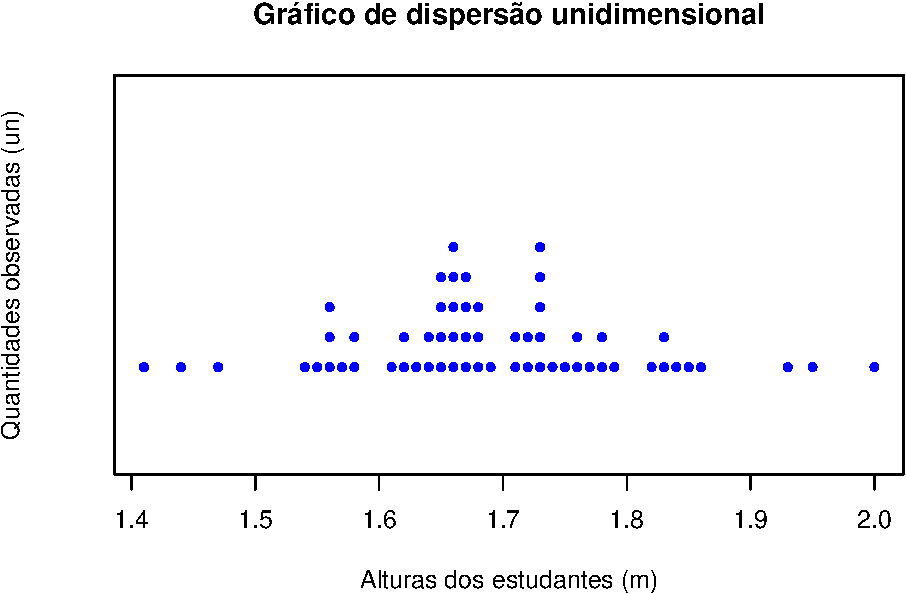
\includegraphics[width=0.8\linewidth]{apostila_files/figure-latex/unnamed-chunk-19-1} 

}

\caption{Gráfico de dispersão unidimensional (stripchart)}\label{fig:unnamed-chunk-19}
\end{figure}

\hypertarget{suxednteses-numuxe9ricas-descritivas}{%
\section{Sínteses numéricas descritivas}\label{suxednteses-numuxe9ricas-descritivas}}

\hfill\break

Além da apresentação elementar de algumas informações relacionadas aos dados brutos da amostra, tais como os valores \emph{mínimo} e \emph{máximo} observados, a estatística descritiva possui muitas outras ferramentas para \emph{condensar} a informação contida nos dados.

\hfill\break

São chamadas de \emph{sínteses numéricas}, medidas que condensam variados aspectos relacionados aos valores dos dados. As principais \emph{sínteses numéricas} são:

\hfill\break

\begin{itemize}
\tightlist
\item
  de tendência central (posição): média (simples ou aritmética, geométrica, harmônica, anarmônica, quadrática, biquadrática), moda e mediana;
\item
  de dispersão (variabilidade): absolutas (amplitude total, variância e desvio padrão) ou relativas (coeficiente de variação, unidades padronizadas); e,
\item
  de subdivisão (separatrizes, quantis): mediana (50\%), quartis (25\%, 50\%, 75\%), decis (10\%, \ldots.90\%) e percentis (1\%\ldots.99\%).
\end{itemize}

\hfill\break

Uma medida de posição ou dispersão é dita \textbf{resistente} quando forem pouco afetadas pela alteração de uma pequena porção dos dados. A mediana é uma medida resistente, já a média e a variância não são.

\hypertarget{medidas-de-tenduxeancia-central-posiuxe7uxe3o}{%
\subsection{Medidas de tendência central (posição)}\label{medidas-de-tenduxeancia-central-posiuxe7uxe3o}}

\hypertarget{muxe9dia}{%
\subsubsection{Média}\label{muxe9dia}}

\hfill\break

Sejam \(x_{1}, x_{2}, ..., x_{n}\) os \(n\) valores assumidos pela variável \(X\) (dados brutos). A \emph{média aritmética simples} será dada por:

\hfill\break

\[
\stackrel{-}{x}=\frac{\sum _{i=1}^{n}{x}_{i}}{n}
\]

\hfill\break

Algumas propriedades da média aritmética:

\hfill\break

\begin{itemize}
\tightlist
\item
  somando-se (ou subtraindo-se) cada um dos elementos do conjunto de dados por uma constante arbitrária qualquer \(k\), a média aritmética ficará adicionada (ou subtraída) dessa essa constante \(k\)
\end{itemize}

\hfill\break

\begin{Shaded}
\begin{Highlighting}[]
\NormalTok{alturas\_ad}\OtherTok{=}\NormalTok{alturas}\FloatTok{+0.05}

\FunctionTok{par}\NormalTok{(}\AttributeTok{mfrow=}\FunctionTok{c}\NormalTok{(}\DecValTok{1}\NormalTok{,}\DecValTok{2}\NormalTok{))}

\FunctionTok{stripchart}\NormalTok{(alturas,}\AttributeTok{method =} \StringTok{"stack"}\NormalTok{,  }\AttributeTok{at=}\FloatTok{0.5}\NormalTok{, }
\AttributeTok{main=}\StringTok{""}\NormalTok{,}\AttributeTok{pch =} \DecValTok{20}\NormalTok{,}
\AttributeTok{col=}\StringTok{"blue"}\NormalTok{, }\AttributeTok{cex=}\DecValTok{1}\NormalTok{, }\AttributeTok{xlab=}\StringTok{"Alturas originais dos estudantes (m)"}\NormalTok{, }
\AttributeTok{ylab=}\StringTok{"Quantidades observadas (un)"}\NormalTok{)}
\FunctionTok{abline}\NormalTok{(}\AttributeTok{v=}\FunctionTok{mean}\NormalTok{(alturas), }\AttributeTok{col=}\StringTok{"red"}\NormalTok{) }
\FunctionTok{text}\NormalTok{(}\FunctionTok{mean}\NormalTok{(alturas)}\SpecialCharTok{{-}}\FloatTok{0.2}\NormalTok{, }\DecValTok{1}\NormalTok{, }\StringTok{"Média=1,69 m"}\NormalTok{, }\AttributeTok{col =} \StringTok{"red"}\NormalTok{, }\AttributeTok{srt=}\DecValTok{90}\NormalTok{) }

\FunctionTok{stripchart}\NormalTok{(alturas\_ad,}\AttributeTok{method =} \StringTok{"stack"}\NormalTok{,  }\AttributeTok{at=}\FloatTok{0.5}\NormalTok{, }
\AttributeTok{main=}\StringTok{""}\NormalTok{,}\AttributeTok{pch =} \DecValTok{20}\NormalTok{,}
\AttributeTok{col=}\StringTok{"blue"}\NormalTok{, }\AttributeTok{cex=}\DecValTok{1}\NormalTok{, }\AttributeTok{xlab=}\StringTok{"Alt. dos estudantes (m) adic. de 5cm"}\NormalTok{, }
\AttributeTok{ylab=}\StringTok{"Quantidades observadas (un)"}\NormalTok{)}
\FunctionTok{abline}\NormalTok{(}\AttributeTok{v=}\FunctionTok{mean}\NormalTok{(alturas\_ad), }\AttributeTok{col=}\StringTok{"red"}\NormalTok{) }
\FunctionTok{text}\NormalTok{(}\FunctionTok{mean}\NormalTok{(alturas\_ad)}\SpecialCharTok{{-}}\FloatTok{0.2}\NormalTok{, }\DecValTok{1}\NormalTok{, }\StringTok{"Média=1,74 m"}\NormalTok{, }\AttributeTok{col =} \StringTok{"red"}\NormalTok{, }\AttributeTok{srt=}\DecValTok{90}\NormalTok{) }
\end{Highlighting}
\end{Shaded}

\begin{figure}

{\centering 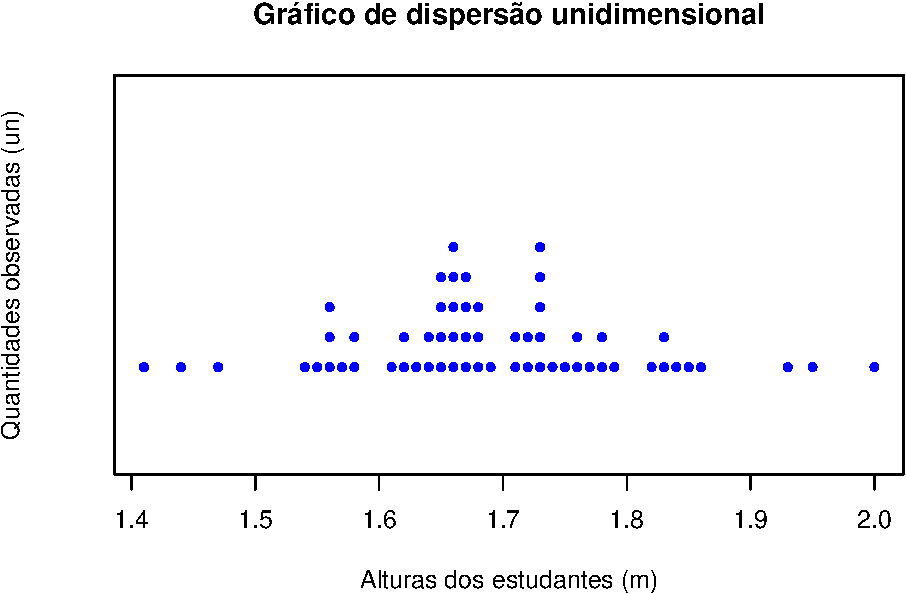
\includegraphics[width=0.8\linewidth]{apostila_files/figure-latex/unnamed-chunk-20-1} 

}

\caption{Mudanças na média pela adição (subtração) de uma constante $k=0.05$}\label{fig:unnamed-chunk-20}
\end{figure}

\hfill\break

\begin{itemize}
\tightlist
\item
  multiplicando-se (ou dividindo-se) cada um dos elementos do conjunto de dados por uma constante arbitrária \(k\), a média aritmética ficará multiplicada (ou dividida) por essa constante \(k\)
\end{itemize}

\hfill\break

\begin{Shaded}
\begin{Highlighting}[]
\NormalTok{alturas\_mult}\OtherTok{=}\NormalTok{alturas}\SpecialCharTok{*}\FloatTok{1.2}

\FunctionTok{par}\NormalTok{(}\AttributeTok{mfrow=}\FunctionTok{c}\NormalTok{(}\DecValTok{1}\NormalTok{,}\DecValTok{2}\NormalTok{))}

\FunctionTok{stripchart}\NormalTok{(alturas,}\AttributeTok{method =} \StringTok{"stack"}\NormalTok{,  }\AttributeTok{at=}\FloatTok{0.5}\NormalTok{, }
\AttributeTok{main=}\StringTok{""}\NormalTok{,}\AttributeTok{pch =} \DecValTok{20}\NormalTok{,}
\AttributeTok{col=}\StringTok{"blue"}\NormalTok{,  }\AttributeTok{xlab=}\StringTok{"Alturas originais dos estudantes (m)"}\NormalTok{, }
\AttributeTok{ylab=}\StringTok{"Quantidades observadas (un)"}\NormalTok{)}
\FunctionTok{abline}\NormalTok{(}\AttributeTok{v=}\FunctionTok{mean}\NormalTok{(alturas), }\AttributeTok{col=}\StringTok{"red"}\NormalTok{) }
\FunctionTok{text}\NormalTok{(}\FunctionTok{mean}\NormalTok{(alturas)}\SpecialCharTok{{-}}\FloatTok{0.1}\NormalTok{, }\DecValTok{1}\NormalTok{, }\StringTok{"Média=1,69 m"}\NormalTok{, }\AttributeTok{col =} \StringTok{"red"}\NormalTok{, }\AttributeTok{srt=}\DecValTok{90}\NormalTok{) }


\FunctionTok{stripchart}\NormalTok{(alturas\_mult,}\AttributeTok{method =} \StringTok{"stack"}\NormalTok{,  }\AttributeTok{at=}\FloatTok{0.5}\NormalTok{, }
\AttributeTok{main=}\StringTok{""}\NormalTok{,}\AttributeTok{pch =} \DecValTok{20}\NormalTok{,}
\AttributeTok{col=}\StringTok{"blue"}\NormalTok{,  }\AttributeTok{xlab=}\StringTok{"Alt. dos estudantes (m) mult. por 1,2"}\NormalTok{, }
\AttributeTok{ylab=}\StringTok{"Quantidades observadas (un)"}\NormalTok{)}
\FunctionTok{abline}\NormalTok{(}\AttributeTok{v=}\FunctionTok{mean}\NormalTok{(alturas\_mult), }\AttributeTok{col=}\StringTok{"red"}\NormalTok{) }
\FunctionTok{text}\NormalTok{(}\FunctionTok{mean}\NormalTok{(alturas\_mult)}\SpecialCharTok{{-}}\FloatTok{0.1}\NormalTok{, }\DecValTok{1}\NormalTok{, }\StringTok{"Média= 2,02 m"}\NormalTok{, }\AttributeTok{col =} \StringTok{"red"}\NormalTok{, }\AttributeTok{srt=}\DecValTok{90}\NormalTok{) }
\end{Highlighting}
\end{Shaded}

\begin{figure}

{\centering 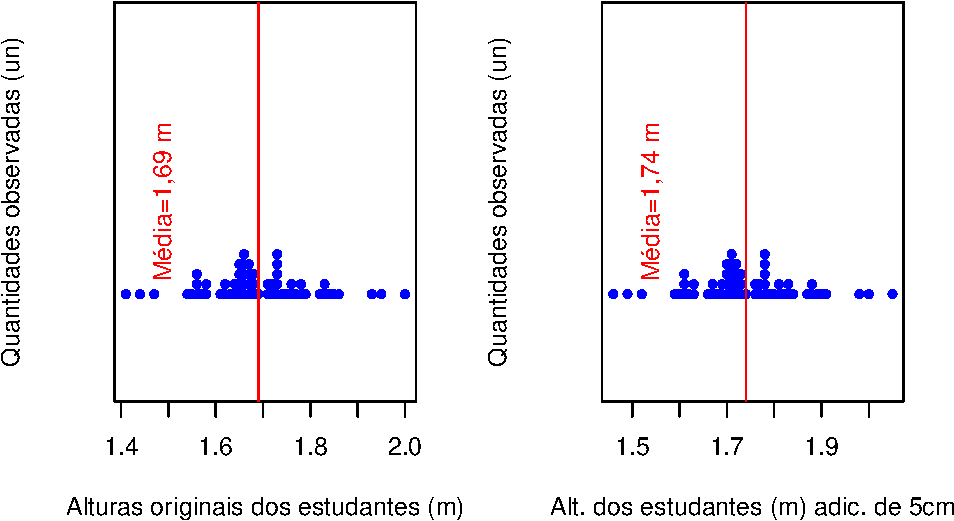
\includegraphics[width=0.8\linewidth]{apostila_files/figure-latex/unnamed-chunk-21-1} 

}

\caption{Mudanças na média pela multiplicação (divisão) de uma constante $k=1.2$}\label{fig:unnamed-chunk-21}
\end{figure}

\hfill\break

\begin{itemize}
\tightlist
\item
  a soma dos desvios observados entre cada um dos valores assumidos pela variável \(X\) e sua média \(\stackrel{-}{x}\) é nula;
\item
  a soma dos quadrados dos desvios é mínima;
\item
  em uma distribuição de frequências, a soma dos produtos dos desvios entre a média o valor médio de cada uma das classes, pelas respectivas frequências é nula; e,
\item
  multiplicando-se (ou dividindo-se) todas as frequências de uma distribuição por uma constante arbitrária, a média aritmética não se altera.
\end{itemize}

\hfill\break

Usando os dados das medidas das alturas dos 60 estudantes teremos o seguinte valor para a \textbf{média}:

\hfill\break

\begin{Shaded}
\begin{Highlighting}[]
\FunctionTok{round}\NormalTok{(}\FunctionTok{mean}\NormalTok{(alturas),}\DecValTok{2}\NormalTok{)}
\end{Highlighting}
\end{Shaded}

\begin{verbatim}
## [1] 1.69
\end{verbatim}

\hypertarget{moda}{%
\subsubsection{Moda}\label{moda}}

\hfill\break

Moda é o valor que ocorre com maior frequência na amostra. Uma amostra pode se apresentar como:

\hfill\break

\begin{itemize}
\tightlist
\item
  unimodal;
\item
  bimodal;
\item
  plurimodal; ou,
\item
  amodal.
\end{itemize}

\hfill\break

\begin{Shaded}
\begin{Highlighting}[]
\NormalTok{tab\_alturas}\OtherTok{=}\FunctionTok{table}\NormalTok{(alturas)}

\NormalTok{tab\_alturas}
\end{Highlighting}
\end{Shaded}

\begin{verbatim}
## alturas
## 1.41 1.44 1.47 1.54 1.55 1.56 1.57 1.58 1.61 1.62 1.63 1.64 1.65 1.66 1.67 1.68 
##    1    1    1    1    1    3    1    2    1    2    1    2    4    5    4    3 
## 1.69 1.71 1.72 1.73 1.74 1.75 1.76 1.77 1.78 1.79 1.82 1.83 1.84 1.85 1.86 1.93 
##    1    2    2    5    1    1    2    1    2    1    1    2    1    1    1    1 
## 1.95    2 
##    1    1
\end{verbatim}

\begin{Shaded}
\begin{Highlighting}[]
\FunctionTok{barplot}\NormalTok{(tab\_alturas,}
        \AttributeTok{main=}\StringTok{"Valores observados da alturas dos estudantes"}\NormalTok{,}
        \AttributeTok{xlab=}\StringTok{"Altura (cm)"}\NormalTok{,}
        \AttributeTok{ylab=}\StringTok{"Quantidade observada (un)"}\NormalTok{,}
        \AttributeTok{ylim=}\FunctionTok{c}\NormalTok{(}\DecValTok{0}\NormalTok{,}\DecValTok{6}\NormalTok{),}
        \AttributeTok{col=}\StringTok{"blue"}\NormalTok{,}
        \AttributeTok{las=}\DecValTok{0}\NormalTok{, }
        \AttributeTok{hor=}\StringTok{"FALSE"}\NormalTok{)}
\end{Highlighting}
\end{Shaded}

\begin{figure}
\centering
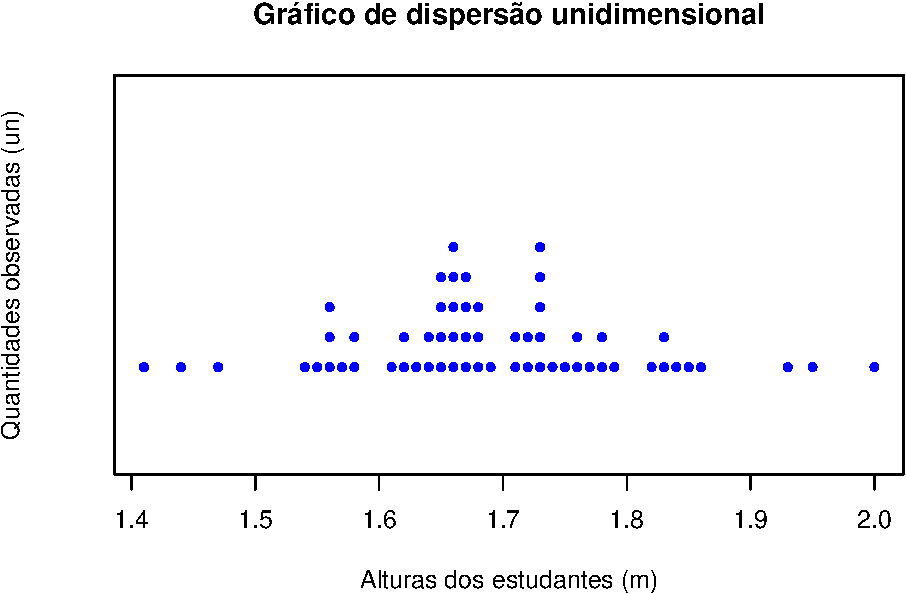
\includegraphics{apostila_files/figure-latex/unnamed-chunk-23-1.pdf}
\caption{\label{fig:unnamed-chunk-23}Bimodal: 1,66 m e 1,73 m}
\end{figure}

\hfill\break

Usando os dados das medidas das alturas dos 60 estudantes teremos os seguintes valores para a \textbf{moda}:

\hfill\break

\begin{Shaded}
\begin{Highlighting}[]
\CommentTok{\# função em R para extrair a moda:}

\NormalTok{Modes }\OtherTok{\textless{}{-}} \ControlFlowTok{function}\NormalTok{(x) \{}
\NormalTok{  ux }\OtherTok{\textless{}{-}} \FunctionTok{unique}\NormalTok{(x)}
\NormalTok{  tab }\OtherTok{\textless{}{-}} \FunctionTok{tabulate}\NormalTok{(}\FunctionTok{match}\NormalTok{(x, ux))}
\NormalTok{  ux[tab }\SpecialCharTok{==} \FunctionTok{max}\NormalTok{(tab)]}
\NormalTok{\}}

\FunctionTok{Modes}\NormalTok{(alturas)}
\end{Highlighting}
\end{Shaded}

\begin{verbatim}
## [1] 1.66 1.73
\end{verbatim}

\hypertarget{mediana}{%
\subsubsection{Mediana}\label{mediana}}

\hfill\break

Mediana é uma medida quantitativa tal que divide a amostra ordenada dos dados em duas partes com \emph{igual quantidade de dados} tais que na primeira delas as observações ossuem valores menores que sua medida e na outra parte as observações possuem valores superiores a ela.

\hfill\break

\begin{figure}

{\centering 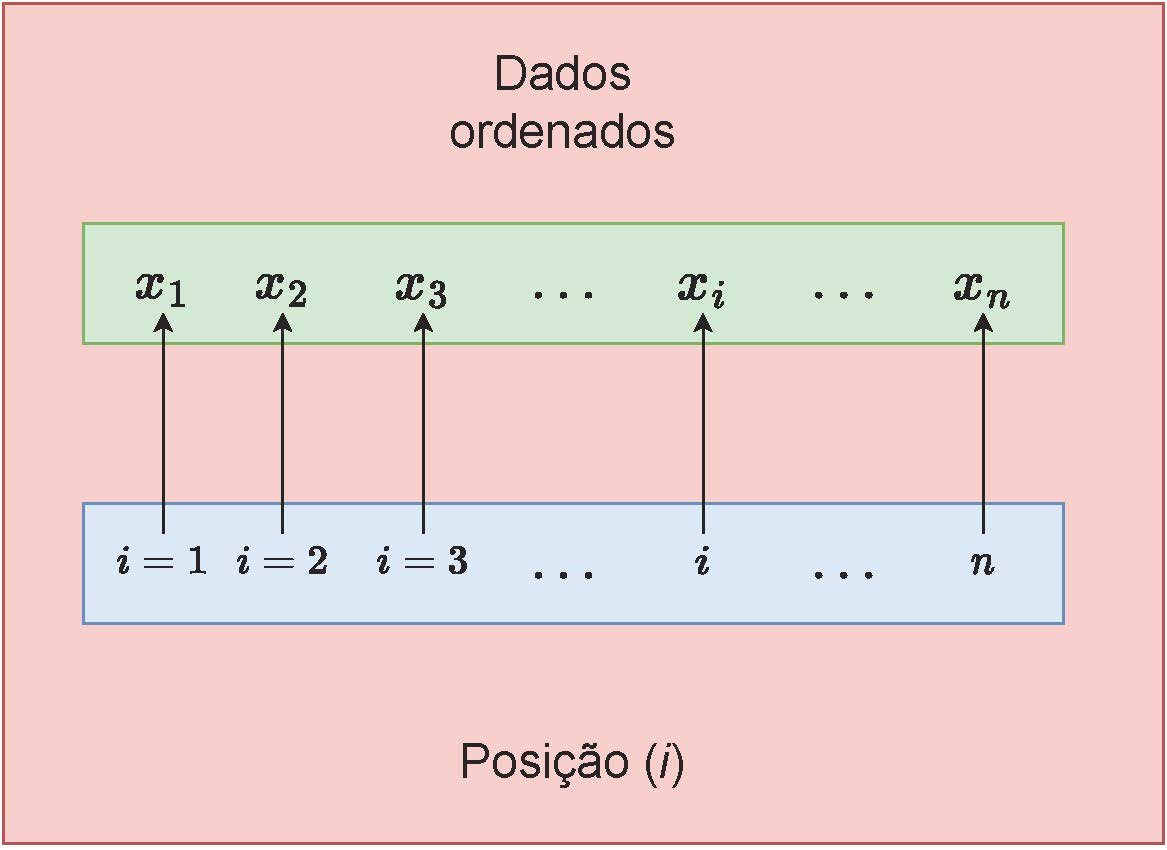
\includegraphics[width=0.5\linewidth]{images3/vetor_posicao} 

}

\caption{Entendendo a indexação de dados}\label{fig:unnamed-chunk-25}
\end{figure}

\hfill\break

Por essa razão, a mediana é uma medida separatriz (de subdivisão) de 50\%, equivalente ao \(2^{o}\) quartil, ao \(5^{o}\) decil e ao \(50^{o}\) percentil. Para sua estimação necessitamos saber qual a \textbf{posição} que ela ocupa no rol de dados e assim, duas situações podem ocorrer:

\hfill\break

1- se a amostra possui um número \textbf{ímpar} (\(n\)) de elementos: a medida da mediana igual ao valor do \(i-ésimo\) elemento da \textbf{amostra ordenada} (a medida da mediana será um valor, de fato, observado) tal que:

\[
Md=x_{i} 
\]\\

com:

\begin{itemize}
\tightlist
\item
  \(i=\frac{n+1}{2}\) (\(n\) é o número de observações);
\end{itemize}

\hfill\break

2- se a amostra possui um número \textbf{par} (\(n\)) de elementos: a medida da mediana será a \textbf{média aritmética} dos valores dos elementos nas posições imediatamente anterior (\(i_{ant}\)) e posterior (\(i_{post}\)) à sua posição central virtual (a medida de mediana não será, portanto, um valor observado):

\hfill\break

\[
Md=média(x_{i_{ant}} ; x_{i_{post}})
\]

\hfill\break

com:

\hfill\break

\begin{itemize}
\tightlist
\item
  \(i_{ant} = \frac{n}{2}\) e \(i_{post} =\frac{n}{2}+1\) (\(n\) é o número de observações).
\end{itemize}

\hfill\break

Sendo uma \textbf{separatriz}, sua posição \(L\) pode ser também calculada pela expressão mais geral (para qualquer percentil) que logo mais será apresentada.

\hfill\break

Mediana para dados apresentados na forma de uma \textbf{distribuição de frequências}:

\hfill\break

\[
Md = l_{inf} + [ \frac{(\frac{n}{2} -  F_{(i_{md}-1)})}{n_{md}} ]\times \Delta_{i}
\]

\hfill\break

onde:

\hfill\break
- \(l_{inf}\): limite inferior da \textbf{classe mediana}: a classe que contem o elemento de ordem \(\frac{n}{2}\);
- \(F_{(i_{md}-1)}\): é a frequência absoluta acumulada até a \textbf{classe anterior à classe mediana};
- \(n_{md}\): é a frequência absoluta da \textbf{classe mediana}; e,
- \(\Delta_{i}\): é o intervalo de cada classe.

\hfill\break

Usando os dados das medidas das alturas dos 60 estudantes teremos o seguinte valor para a \textbf{mediana}:

\hfill\break

\begin{Shaded}
\begin{Highlighting}[]
\FunctionTok{sort}\NormalTok{(alturas)}
\end{Highlighting}
\end{Shaded}

\begin{verbatim}
##  [1] 1.41 1.44 1.47 1.54 1.55 1.56 1.56 1.56 1.57 1.58 1.58 1.61 1.62 1.62 1.63
## [16] 1.64 1.64 1.65 1.65 1.65 1.65 1.66 1.66 1.66 1.66 1.66 1.67 1.67 1.67 1.67
## [31] 1.68 1.68 1.68 1.69 1.71 1.71 1.72 1.72 1.73 1.73 1.73 1.73 1.73 1.74 1.75
## [46] 1.76 1.76 1.77 1.78 1.78 1.79 1.82 1.83 1.83 1.84 1.85 1.86 1.93 1.95 2.00
\end{verbatim}

\begin{Shaded}
\begin{Highlighting}[]
\FunctionTok{median}\NormalTok{(alturas)}
\end{Highlighting}
\end{Shaded}

\begin{verbatim}
## [1] 1.675
\end{verbatim}

\hfill\break

\hypertarget{diferentes-posiuxe7uxf5es-da-muxe9dia-moda-e-mediana}{%
\subsubsection{Diferentes posições da média, moda e mediana}\label{diferentes-posiuxe7uxf5es-da-muxe9dia-moda-e-mediana}}

\hfill\break

Essas três medidas podem se apresentar com valores em posições alternadas quando as comparamos:\\

\begin{itemize}
\tightlist
\item
  quando a moda=mediana=média temos uma distribuição de frequências razoavelmente \textbf{simétrica};
\item
  quando a moda \(\leq\) mediana \(\leq\) média (há uma quantidade maior de dados com grandes valores, arrastando a média para a direita, para cima) temos uma distribuição de frequências \textbf{positivamente assimétrica}, ; e,\\
\item
  quando a moda \(\geq\) mediana \(\geq\) média (há uma quantidade maior de dados com pequenos valores, arrastando a média para a esquerda, para baixo) temos uma distribuição de frequências \textbf{negativamente assimétrica}.
\end{itemize}

\hfill\break

\hfill\break

\begin{Shaded}
\begin{Highlighting}[]
\FunctionTok{barplot}\NormalTok{(tab\_alturas,}
        \AttributeTok{main=}\StringTok{"Valores observados da alturas dos estudantes"}\NormalTok{,}
        \AttributeTok{xlab=}\StringTok{"Altura (cm)"}\NormalTok{,}
        \AttributeTok{ylab=}\StringTok{"Quantidade observada (un)"}\NormalTok{,}
        \AttributeTok{ylim=}\FunctionTok{c}\NormalTok{(}\DecValTok{0}\NormalTok{,}\DecValTok{6}\NormalTok{),}
        \AttributeTok{col=}\StringTok{"blue"}\NormalTok{,}
        \AttributeTok{las=}\DecValTok{0}\NormalTok{, }
        \AttributeTok{hor=}\StringTok{"FALSE"}\NormalTok{)}
\FunctionTok{abline}\NormalTok{(}\AttributeTok{v=}\FunctionTok{mean}\NormalTok{(}\FloatTok{19.9}\NormalTok{, }\FloatTok{21.1}\NormalTok{), }\AttributeTok{col=}\StringTok{"red"}\NormalTok{)}
\FunctionTok{text}\NormalTok{( }\FunctionTok{mean}\NormalTok{(}\FloatTok{19.9}\NormalTok{, }\FloatTok{21.1}\NormalTok{)}\SpecialCharTok{{-}}\FloatTok{0.5}\NormalTok{, }\DecValTok{5}\NormalTok{, }\StringTok{"Média=1,69 m"}\NormalTok{, }\AttributeTok{col =} \StringTok{"red"}\NormalTok{, }\AttributeTok{srt=}\DecValTok{90}\NormalTok{)}
\FunctionTok{abline}\NormalTok{(}\AttributeTok{v=}\FunctionTok{median}\NormalTok{(}\FloatTok{18.7}\NormalTok{ , }\FloatTok{19.9}\NormalTok{), }\AttributeTok{col=}\StringTok{"darkgreen"}\NormalTok{) }
\FunctionTok{text}\NormalTok{(}\FunctionTok{median}\NormalTok{(}\FloatTok{18.7}\NormalTok{ , }\FloatTok{19.9}\NormalTok{)}\SpecialCharTok{{-}}\FloatTok{0.5}\NormalTok{, }\DecValTok{5}\NormalTok{, }\StringTok{"Mediana=1,675 m"}\NormalTok{, }\AttributeTok{col =} \StringTok{"darkgreen"}\NormalTok{, }\AttributeTok{srt=}\DecValTok{90}\NormalTok{)}
\FunctionTok{abline}\NormalTok{(}\AttributeTok{v=}\FunctionTok{c}\NormalTok{(}\FloatTok{16.3}\NormalTok{, }\FloatTok{23.5}\NormalTok{), }\AttributeTok{col=}\StringTok{"darkgrey"}\NormalTok{) }
\FunctionTok{text}\NormalTok{(}\FunctionTok{c}\NormalTok{(}\FloatTok{16.3{-}0.5}\NormalTok{, }\FloatTok{23.5{-}0.5}\NormalTok{), }\DecValTok{5}\NormalTok{, }\FunctionTok{c}\NormalTok{(}\StringTok{"Moda=1,66"}\NormalTok{,}\StringTok{"Moda=1,73"}\NormalTok{), }\AttributeTok{col =} \StringTok{"darkgray"}\NormalTok{, }\AttributeTok{srt=}\DecValTok{90}\NormalTok{)}
\end{Highlighting}
\end{Shaded}

\begin{figure}

{\centering 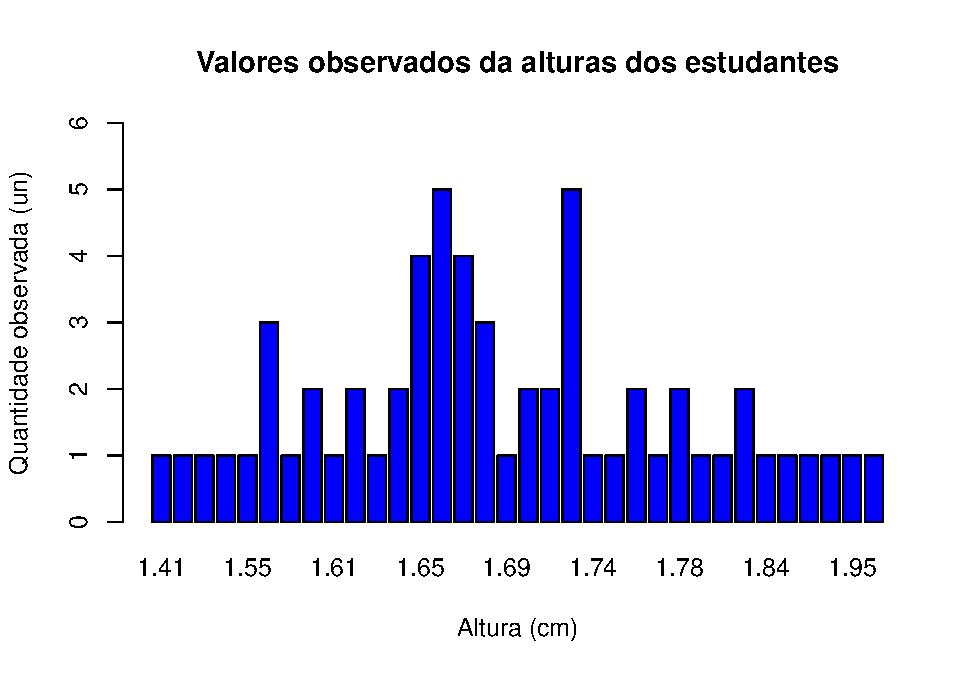
\includegraphics[width=0.8\linewidth]{apostila_files/figure-latex/unnamed-chunk-28-1} 

}

\caption{Valores observados das alturas dos estudantes e as posições da média, moda e mediana}\label{fig:unnamed-chunk-28}
\end{figure}

\hfill\break

\begin{figure}

{\centering 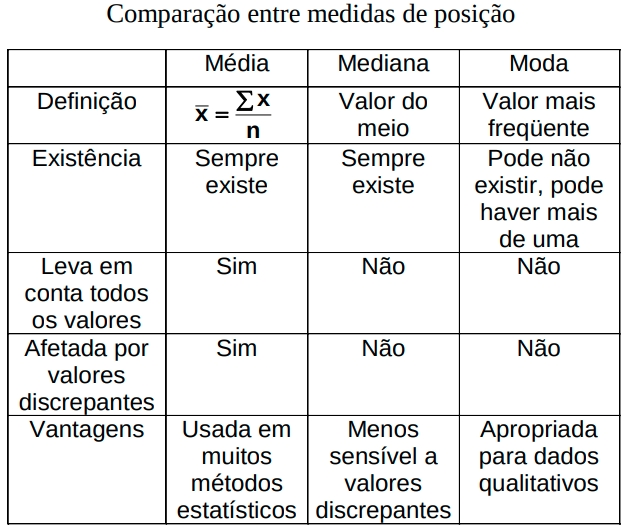
\includegraphics[width=0.8\linewidth]{images3/comp_sinteses} 

}

\caption{Quadro comparativo entre as medidas de tendência central (posição)}\label{fig:unnamed-chunk-29}
\end{figure}

\hypertarget{medidas-de-dispersuxe3o-variabilidade}{%
\subsection{Medidas de dispersão (variabilidade)}\label{medidas-de-dispersuxe3o-variabilidade}}

\hfill\break

O conhecimento de uma medida de tendência central nos provê uma informação útil mas incompleta. As medidas de dispersão nos ajudam a ter uma perspectiva melhor dos dados.

\hfill\break

\begin{itemize}
\tightlist
\item
  amplitude total dos dados;
\item
  desvio padrão (variância): é considerada a mais útil das medidas de dispersão;\\
\item
  coeficiente de variação; e,
\item
  unidades padronizadas.
\end{itemize}

\hfill\break

Diferentes tipos quanto à dimensão (unidade):

\hfill\break

\begin{itemize}
\tightlist
\item
  \textbf{medidas absolutas} são aquelas expressas na mesma unidade de medida da variável do fenômeno estudado (\(m;kg;\frac{R\$}{mês};\dots\));\\
\item
  \textbf{medidas relativas} são adimiensionais e assim podem ser usadas para se comparar a variabilidade de dois ou mais conjuntos de dados, mesmo quando as variáveis se refiram a diferentes fenômenos ou que sejam expressas, originalmente, em diferentes unidades.
\end{itemize}

\hfill\break

\hypertarget{amplitude-total-dos-dados}{%
\subsubsection{Amplitude total dos dados}\label{amplitude-total-dos-dados}}

\hfill\break

A amplitude total dos dados é a simples diferença entre o \textbf{maior} e o \textbf{menor} dos valores observados:

\hfill\break

\[
A=x_{max} - x_{min}
\]

\hfill\break

\hypertarget{estimauxe7uxe3o-da-variuxe2ncia-e-desvio-padruxe3o}{%
\subsubsection{Estimação da variância (e desvio padrão)}\label{estimauxe7uxe3o-da-variuxe2ncia-e-desvio-padruxe3o}}

\hfill\break

Sejam \(x_{1}, x_{2}, ..., x_{n}\) os \(n\) valores assumidos pela variável \(X\). Dá-se o nome de desvios a contar da média as diferenças entre cada uma das observações e a média: \(x_{i} - \stackrel{-}{x}\) com \(i=1,2,...,n\).

\hfill\break

Não é possível considerar a possibilidade de se adotar o valor médio desses desvios pois uma das propriedades da média é que a soma dos desvios em torno de si é nula.

\hfill\break

\[
\stackrel{-}{d} = \frac{\sum _{i=1}^{n}\left(x_{i}-\stackrel{-}{x}\right)}{n}
\]
\[
\sum _{i=1}^{n}\left(x_{i}-\stackrel{-}{x}\right)=0
\]

\hfill\break

constitui-se numa restrição linear dos desvios porque qualquer \(n-1\) deles completamente determina o outro. Tampouco se considera a possibilidade de se adotar o valor médio desses desvios em módulo, pelas dificuldades teóricas em problemas de inferência.

\hfill\break

\[
\stackrel{-}{d}  = \frac{\sum _{i=1}^{n}\left|x_{i}-\stackrel{-}{x}\right|}{n}
\]

\hfill\break

Uma alternativa é adotar o valor médio do \textbf{quadrado} desses desvios.

\hfill\break

\[
S^{2}=\frac{\sum _{i=1}^{n}\left(x_{i}-\stackrel{-}{x}\right)^{2}}{n-1}
\]

\hfill\break

ou,

\hfill\break

\[
S^{2}=\frac{1}{(n-1)} \times \left[ \sum _{i=1}^{n} (x_{i}^{2}) - \frac{({\sum _{i=1}^{n}x_{i})}^{2} }{n}\right]
\]

\hfill\break

Diz-se que a variância amostral (variância \emph{ajustada}) possui \((n-1)\) graus de liberdade, denotado pela letra grega \(\nu\). A perda de \emph{um} grau de liberdade deve-se à necessidade de se substituir a média populacional desconhecida (\(\mu\)) por sua estimativa amostral (\(\stackrel{-}{x}\)), deduzida a partir dos dados coletados.

\hfill\break

Pode-se demonstrar que em razão dessa restrição a melhor estimativa para a variância populacional é obtida dividindo-se a soma dos quadrados dos desvios por \((n-1)\). Assim \(S^{2}\) será um estimador não tendencioso para a variância amostral ao ser dividido por \((n-1)\)\}.

\hfill\break

Uma medida de dispersão que apresenta a mesma unidade que a das observações originais é o \textbf{desvio-padrão}, definido como a raiz quadrada positiva da variância.

\hfill\break

\[
S= \sqrt{\frac{\sum _{i=1}^{n}\left(x_{i}-\stackrel{-}{x}\right)^{2}}{n-1}}
\]

\hfill\break

Tanto a variância quanto o desvio padrão indicam, em média, qual será o erro (desvio) cometido ao tentar substituir cada observação pela medida resumo do conjunto de dados (média).

\hfill\break

Usando os dados das medidas das alturas dos 60 estudantes teremos o seguinte valor para a \textbf{variância} (com unidade igual a \(m^{2}\)) e o \textbf{desvio padrão} (com unidade igual a \(m\):

\hfill\break

\begin{Shaded}
\begin{Highlighting}[]
\CommentTok{\# Variãncia}
\FunctionTok{var}\NormalTok{(alturas)}
\end{Highlighting}
\end{Shaded}

\begin{verbatim}
## [1] 0.0130809
\end{verbatim}

\begin{Shaded}
\begin{Highlighting}[]
\CommentTok{\# Desvio padrão}
\FunctionTok{sd}\NormalTok{(alturas) }
\end{Highlighting}
\end{Shaded}

\begin{verbatim}
## [1] 0.1143718
\end{verbatim}

Propriedades da variância:

\hfill\break

\begin{itemize}
\tightlist
\item
  somando-se (ou subtraindo-se) cada um dos elementos do conjunto de dados por uma constante arbitrária, a variância (e o desvio padrão) não se altera; e,
\item
  multiplicando-se (ou dividindo-se) cada um dos elementos do conjunto de dados por uma constante arbitrária, a variância ficará multiplicada (ou dividida) pelo quadrado dessa constante. O desvio padrão fica multiplicado (ou dividido) por essa constante
\end{itemize}

\hfill\break

\begin{Shaded}
\begin{Highlighting}[]
\CommentTok{\# Adicionando{-}se uma constante k=0.05}
\NormalTok{alturas\_ad}\OtherTok{=}\NormalTok{alturas}\FloatTok{+0.05}

\CommentTok{\# Variância não se altera}
\NormalTok{var\_ad}\OtherTok{=} \FunctionTok{var}\NormalTok{(alturas\_ad)}
\NormalTok{var\_ad}
\end{Highlighting}
\end{Shaded}

\begin{verbatim}
## [1] 0.0130809
\end{verbatim}

\begin{Shaded}
\begin{Highlighting}[]
\CommentTok{\# Multiplicando{-}se uma constante k=1.2}
\NormalTok{alturas\_mult}\OtherTok{=}\NormalTok{alturas}\SpecialCharTok{*}\FloatTok{1.2}

\CommentTok{\# Variância fica multiplicada (dividida) pelo quadrado dessa constante)}
\FunctionTok{var}\NormalTok{(alturas\_mult)}
\end{Highlighting}
\end{Shaded}

\begin{verbatim}
## [1] 0.0188365
\end{verbatim}

\begin{Shaded}
\begin{Highlighting}[]
\FunctionTok{all.equal}\NormalTok{(}\FunctionTok{var}\NormalTok{(alturas\_mult), }\FunctionTok{var}\NormalTok{(alturas)}\SpecialCharTok{*}\NormalTok{(}\FloatTok{1.2}\SpecialCharTok{\^{}}\DecValTok{2}\NormalTok{)) }
\end{Highlighting}
\end{Shaded}

\begin{verbatim}
## [1] TRUE
\end{verbatim}

\hypertarget{coeficiente-de-variauxe7uxe3o.}{%
\subsubsection{Coeficiente de variação.}\label{coeficiente-de-variauxe7uxe3o.}}

\hfill\break

O coeficiente de variação (uma medida adimensional) é dado pela razão do desvio padrão pela média:

\hfill\break

\[
CV(\%)= 100\cdot(\frac{s}{\stackrel{-}{x}})
\]

\hfill\break

\begin{table}[h]
\centering
\caption{Classificação da variabilidade a partir da medida do Coeficiente de variação}
\begin{tabular}{|c|c|}
\hline 
Classificação  & Medida do Coeficiente de variação (CV \%) \\ 
\hline 
Baixo & $CV \le 10\%$ \\
\hline 
Médio  & $10\% \le CV \le 20\%$ \\
\hline 
Alto  & $20\% \le CV \le 30\%$ \\
\hline 
Muito alto & $CV \ge 30\%$ \\
\hline 
\end{tabular}
\end{table}

\hfill\break

\hypertarget{padronizauxe7uxe3o-z-scores}{%
\subsubsection{\texorpdfstring{Padronização (\emph{z-scores})}{Padronização (z-scores)}}\label{padronizauxe7uxe3o-z-scores}}

\hfill\break

À conversão do valor assumido por uma variável em unidades de desvio padrão acima (ou abaixo) do valor médio de sua distribuição é dado o nome de \emph{padronização}. Essa métrica permite comparações com outras, procedentes de outros fenômenos.

\hfill\break

Para padronizar (achar o seu \emph{z-score} Z) o valor de uma variável procede-se segundo a fórmula:

\hfill\break

\[
Z=\frac{x_{i} - \stackrel{-}{x}}{s}
\]

\hfill\break
O valor \(Z\) expressa quantos desvios esse dado está acima (ou abaixo) da média da distribuição.

\hfill\break

Pelo \emph{Teorema de Tchebichev} pode-se estimar a probabilidade mínima dos dados situados a certa distância de \(k\) desvios da média dessa distribuição:

\hfill\break

\[
P(|X-\mu|\ge k\sigma) \leq 1 - \frac{1}{k^{2}}
\]

\hfill\break

Assim, se \(k=2\) \textbf{ao menos} 75\% das observações devem estar entre a média e dois desvios padrões acima ou abaixo da média.

\hfill\break

\begin{Shaded}
\begin{Highlighting}[]
\NormalTok{med}\OtherTok{=}\FunctionTok{round}\NormalTok{(}\FunctionTok{mean}\NormalTok{(alturas),}\DecValTok{2}\NormalTok{)}
\NormalTok{desv}\OtherTok{=} \FunctionTok{round}\NormalTok{(}\FunctionTok{sd}\NormalTok{(alturas),}\DecValTok{2}\NormalTok{)}
\end{Highlighting}
\end{Shaded}

\hfill\break

No exemplo das alturas dos estudantes temos a média de 1.69 m e um desvio padrão de 0.11 m. Assim, \textbf{ao menos} 75\% das alturas deverão estar entre 1.47 m e 1.91 m.

\hfill\break

\begin{Shaded}
\begin{Highlighting}[]
\FunctionTok{sort}\NormalTok{(alturas)}
\end{Highlighting}
\end{Shaded}

\begin{verbatim}
##  [1] 1.41 1.44 1.47 1.54 1.55 1.56 1.56 1.56 1.57 1.58 1.58 1.61 1.62 1.62 1.63
## [16] 1.64 1.64 1.65 1.65 1.65 1.65 1.66 1.66 1.66 1.66 1.66 1.67 1.67 1.67 1.67
## [31] 1.68 1.68 1.68 1.69 1.71 1.71 1.72 1.72 1.73 1.73 1.73 1.73 1.73 1.74 1.75
## [46] 1.76 1.76 1.77 1.78 1.78 1.79 1.82 1.83 1.83 1.84 1.85 1.86 1.93 1.95 2.00
\end{verbatim}

\begin{Shaded}
\begin{Highlighting}[]
\CommentTok{\# Duas observações menores que 1,47m e trẽs maiores que 1,91m.}
\CommentTok{\# Assim, 54 observações dentro do intervalo, equivalendo a 91,66\% do total.}
\end{Highlighting}
\end{Shaded}

\hypertarget{medidas-de-subdivisuxe3o-separatrizes}{%
\subsection{Medidas de subdivisão (separatrizes)}\label{medidas-de-subdivisuxe3o-separatrizes}}

\hfill\break

Separatrizes (quantis) são valores que delimitam uma proporção de observações existentes de um conjunto de dados previamente ordenados menores que ele. Os quantis mais expressivos são:

\hfill\break

\begin{itemize}
\tightlist
\item
  1\(^{o}\) Quartil (\(q_{0,25}\)): 25\% dos dados possuem valores abaixo desse valor e 75\% estão acima;
\item
  2\(^{o}\) Quartil ou mediana (\(q_{0,50}\)): 50\% dos dados possuem valores abaixo desse valor e 50\% estão acima; e,
\item
  3\(^{o}\) Quartil (\(q_{0,75}\)): 75\% dos dados possuem valores abaixo desse valor e 25\% estão acima.
\end{itemize}

\hfill\break

De modo geral, um \emph{quantil} de ordem \(p\) (ou também \(p-quantil\), indicado por \(q_{p}\)) é uma medida onde \(p\) é uma proporção qualquer (limitada no intervalo 0 \textless{} p \textless{} 1), tal que 100\(p\)\% das observações sejam menores que seu valor \(q_{p}\). Um importante gráfico que mais adiante será exposto em detalhes é o \emph{Boxplot} que, além da mediana, para sua confecção necessitamos de duas outras separatrizes: o 1\(^{o}\) e 3\(^{o}\) quartis. \textbackslash{}

\hfill\break
Há muitos modos de se estabelecer os quantis descritos na literatura. O próprio \href{https://www.rdocumentation.org/packages/stats/versions/3.6.2/topics/quantile}{R} apresenta 9 modos diferentes:

\hfill\break

\begin{Shaded}
\begin{Highlighting}[]
\FunctionTok{quantile}\NormalTok{(alturas, }\AttributeTok{type=}\DecValTok{1}\NormalTok{)}
\end{Highlighting}
\end{Shaded}

\begin{verbatim}
##   0%  25%  50%  75% 100% 
## 1.41 1.63 1.67 1.75 2.00
\end{verbatim}

\begin{Shaded}
\begin{Highlighting}[]
\FunctionTok{quantile}\NormalTok{(alturas, }\AttributeTok{type=}\DecValTok{2}\NormalTok{)}
\end{Highlighting}
\end{Shaded}

\begin{verbatim}
##    0%   25%   50%   75%  100% 
## 1.410 1.635 1.675 1.755 2.000
\end{verbatim}

\begin{Shaded}
\begin{Highlighting}[]
\FunctionTok{quantile}\NormalTok{(alturas, }\AttributeTok{type=}\DecValTok{3}\NormalTok{)}
\end{Highlighting}
\end{Shaded}

\begin{verbatim}
##   0%  25%  50%  75% 100% 
## 1.41 1.63 1.67 1.75 2.00
\end{verbatim}

\begin{Shaded}
\begin{Highlighting}[]
\FunctionTok{quantile}\NormalTok{(alturas, }\AttributeTok{type=}\DecValTok{4}\NormalTok{)}
\end{Highlighting}
\end{Shaded}

\begin{verbatim}
##   0%  25%  50%  75% 100% 
## 1.41 1.63 1.67 1.75 2.00
\end{verbatim}

\begin{Shaded}
\begin{Highlighting}[]
\FunctionTok{quantile}\NormalTok{(alturas, }\AttributeTok{type=}\DecValTok{5}\NormalTok{)}
\end{Highlighting}
\end{Shaded}

\begin{verbatim}
##    0%   25%   50%   75%  100% 
## 1.410 1.635 1.675 1.755 2.000
\end{verbatim}

\begin{Shaded}
\begin{Highlighting}[]
\FunctionTok{quantile}\NormalTok{(alturas, }\AttributeTok{type=}\DecValTok{6}\NormalTok{)}
\end{Highlighting}
\end{Shaded}

\begin{verbatim}
##     0%    25%    50%    75%   100% 
## 1.4100 1.6325 1.6750 1.7575 2.0000
\end{verbatim}

\begin{Shaded}
\begin{Highlighting}[]
\FunctionTok{quantile}\NormalTok{(alturas, }\AttributeTok{type=}\DecValTok{7}\NormalTok{)}
\end{Highlighting}
\end{Shaded}

\begin{verbatim}
##     0%    25%    50%    75%   100% 
## 1.4100 1.6375 1.6750 1.7525 2.0000
\end{verbatim}

\begin{Shaded}
\begin{Highlighting}[]
\FunctionTok{quantile}\NormalTok{(alturas, }\AttributeTok{type=}\DecValTok{8}\NormalTok{)}
\end{Highlighting}
\end{Shaded}

\begin{verbatim}
##       0%      25%      50%      75%     100% 
## 1.410000 1.634167 1.675000 1.755833 2.000000
\end{verbatim}

\begin{Shaded}
\begin{Highlighting}[]
\FunctionTok{quantile}\NormalTok{(alturas, }\AttributeTok{type=}\DecValTok{9}\NormalTok{)}
\end{Highlighting}
\end{Shaded}

\begin{verbatim}
##       0%      25%      50%      75%     100% 
## 1.410000 1.634375 1.675000 1.755625 2.000000
\end{verbatim}

~

Para grandes conjuntos de dados a diferença entre os quantis determinados sob esses diferentes modos será despresível. De modo geral, para se calcular a posição \emph{L} de um quantil qualquer de ordem \emph{p} em um rol de dados pode-se usar a seguinte regra empírica:

\[
L_{p}=\frac{p}{100} \times (n+1)
\]\\

Onde:

\hfill\break

\begin{itemize}
\tightlist
\item
  \emph{p} é a \textbf{ordem} do quantil em \% (50\% no caso mediana, por exemplo);
\item
  \emph{n} é o número de dados do rol; e,
\item
  \emph{L} é a \textbf{posição} do valor referente ao quantil desejado.
\end{itemize}

\hfill\break

\hfill\break

Assim, para a determinação dos quartis, o valor de \emph{p} seria:

\hfill\break

\begin{itemize}
\tightlist
\item
  para o \emph{primeiro quartil} (\(Q_{1}\)): \(L_{q_{0,25}}=\frac{25}{100} \times (n+1)\);
\item
  para o \emph{segundo quartil} (a mediana ou \(Q_{2}\)): \(L_{q_{0,50}}=\frac{50}{100} \times (n+1)\); ou,\\
\item
  para o \emph{terceiro quartil} (\(Q_{3}\)): \(L_{q_{0,75}}=\frac{75}{100} \times (n+1)\).
\end{itemize}

\hfill\break

Novamente podemos nos deparar com \textbf{duas situações possíveis} para o valor calculado para a posição \emph{L}:

\hfill\break

\begin{figure}

{\centering 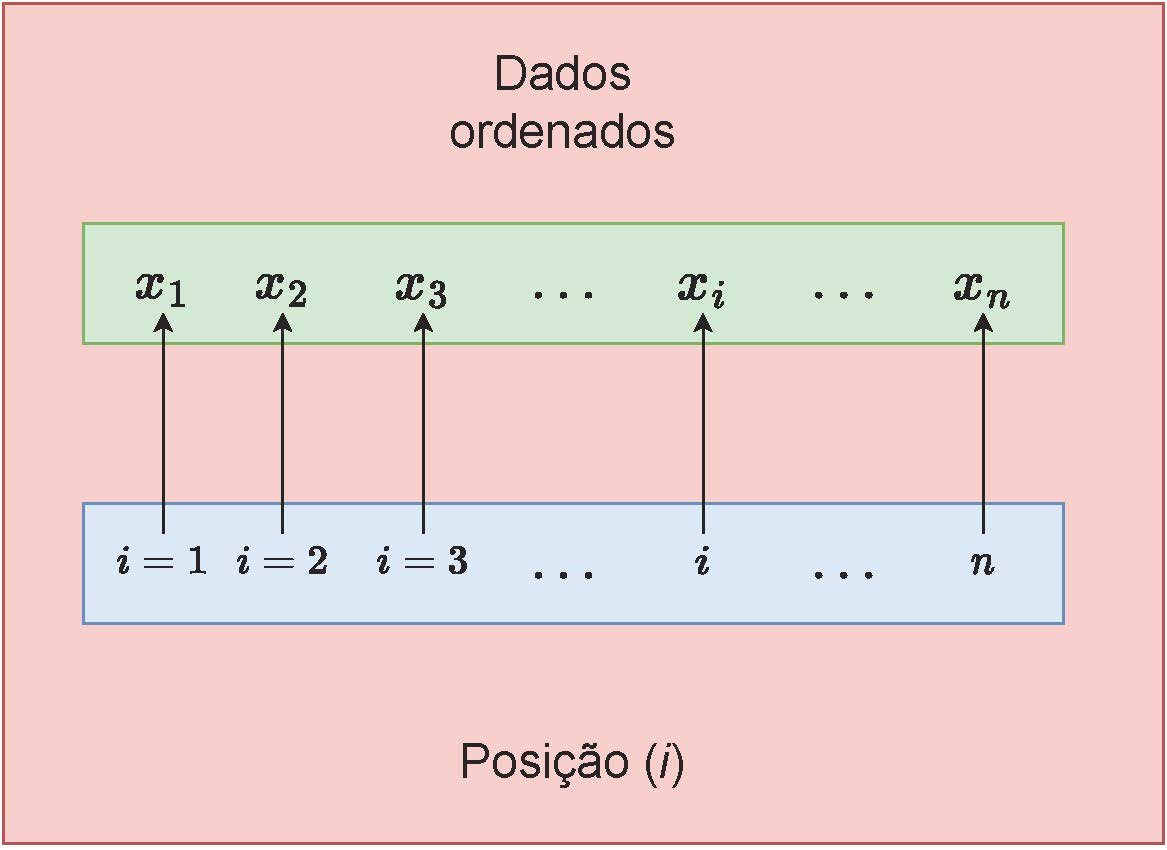
\includegraphics[width=0.6\linewidth]{images3/vetor_posicao} 

}

\caption{Entendendo a indexação de dados}\label{fig:unnamed-chunk-36}
\end{figure}

\hfill\break

\begin{itemize}
\tightlist
\item
  se valor calculado da \textbf{posição} L for um inteiro, essa será a posição onde encontraremos o valor referente ao quantil desejado;\\
\item
  se o valor calculado da \textbf{posição L} for fracionário, o valor desse quantil será determinado pela média entre os dois valores dos dados que estão nas \textbf{posições} imediatamente anterior e imediatamente posterior à posição \textbf{L} calculada.
\end{itemize}

\hfill\break

Juntamente com as observações mínima (\(x_{i}\)) e máxima (\(x_{n}\)), o 1\(^{o}\), 2\(^{o}\) e 3\(^{o}\) Quartis são importantes para se ter uma boa idéia da assimetria da distribuição dos dados.

\hfill\break

Para uma distribuição simétrica (ou aproximadamente simétrica) deveremos observar (Distribuição Gaussiana):

\hfill\break

\begin{itemize}
\tightlist
\item
  a dispersão inferior: \(q_{2} - x_{1} \approx x_{n} - q_{2}\) à dispersão superior ;
\item
  \(q_{2} - q_{1} \approx q_{3} - q_{2}\); e,
\item
  \(q_{1} - x_{1} \approx x_{n} - q_{3}\).
\end{itemize}

\hfill\break

Para nosso conjunto de dados, segundo a regra empírica apresentada teremos as seguintes posições para determinação dos valores dos quartis:

\hfill\break

\begin{itemize}
\tightlist
\item
  para o \emph{primeiro quartil}:
\end{itemize}

\begin{align*}
L_{Q_{1}} & =\frac{p}{100} \times (n+1) \\
          & =\frac{25}{100} \times (60+1) \\
          & = 0,25*61 \\
          & = 15,25
\end{align*}\\

\begin{itemize}
\tightlist
\item
  para o \emph{segundo quartil}:
\end{itemize}

\begin{align*}
L_{Q_{2}} & =\frac{p}{100} \times (n+1) \\
          & =\frac{50}{100} \times (60+1) \\
          & = 0,5*61 \\
          & = 30,5
\end{align*}

\hfill\break
- para o \emph{terceiro quartil}:

\begin{align*}
L_{Q_{3}} & =\frac{p}{100} \times (n+1) \\
          & =\frac{75}{100} \times (60+1) \\
          & = 0,75*61 \\
          & = 45,75
\end{align*}

\hfill\break

E os quartis serão:

\hfill\break

-\(Q_{1}\)=1,635
-\(Q_{2}\)=1,675
-\(Q_{3}\)=1,755

\hfill\break

\hypertarget{medidas-de-forma-assimetria-curtose}{%
\section{Medidas de forma (assimetria \& curtose)}\label{medidas-de-forma-assimetria-curtose}}

\hfill\break

Quando analisamos o histograma (a representação gráfica da distribuição das frequências dos valores agrupados em classes) de uma determinada variável, não é muito comum que ele se mostre simétrico tal como seria se os dados fossem distribuídos de modo exatamente Normal.

\hfill\break

Ao observarmos que a cauda se mostra mais alongada para a direita (indicativo da existência de uma quantidade maior de dados com grandes valores, \emph{arrastando} a média para a direita: moda \(<\) mediana \(<\) média) diz-se que a \emph{distribuição é assimétrica à direita}. Na situação oposta (moda \(>\) mediana \(>\) média) diz-se que ela é \emph{assimétrica à esquerda}.

\hfill\break

\begin{Shaded}
\begin{Highlighting}[]
\NormalTok{a}\OtherTok{=}\FunctionTok{rbeta}\NormalTok{(}\DecValTok{10000}\NormalTok{,}\DecValTok{5}\NormalTok{,}\DecValTok{2}\NormalTok{)}
\NormalTok{c}\OtherTok{=}\FunctionTok{rbeta}\NormalTok{(}\DecValTok{10000}\NormalTok{,}\DecValTok{5}\NormalTok{,}\DecValTok{5}\NormalTok{)}
\NormalTok{b}\OtherTok{=}\FunctionTok{rbeta}\NormalTok{(}\DecValTok{10000}\NormalTok{,}\DecValTok{2}\NormalTok{,}\DecValTok{5}\NormalTok{)}

\FunctionTok{par}\NormalTok{(}\AttributeTok{mfrow=}\FunctionTok{c}\NormalTok{(}\DecValTok{1}\NormalTok{,}\DecValTok{3}\NormalTok{))}
\FunctionTok{hist}\NormalTok{(a, }
     \AttributeTok{xlab=}\StringTok{"Valores"}\NormalTok{,}\AttributeTok{col =} \StringTok{\textquotesingle{}lightblue\textquotesingle{}}\NormalTok{,}
     \AttributeTok{ylab=}\StringTok{"Frequência"}\NormalTok{,}
     \AttributeTok{main=}\StringTok{"Assimetria à esq."}\NormalTok{)}
\FunctionTok{hist}\NormalTok{(c, }
     \AttributeTok{xlab=}\StringTok{"Valores"}\NormalTok{,}\AttributeTok{col =} \StringTok{\textquotesingle{}lightblue\textquotesingle{}}\NormalTok{,}
     \AttributeTok{ylab=}\StringTok{"Frequência"}\NormalTok{,}
     \AttributeTok{main=}\StringTok{"Relativa simetria"}\NormalTok{)}
\FunctionTok{hist}\NormalTok{(b, }
     \AttributeTok{xlab=}\StringTok{"Valores"}\NormalTok{,}\AttributeTok{col =} \StringTok{\textquotesingle{}lightblue\textquotesingle{}}\NormalTok{,}
     \AttributeTok{ylab=}\StringTok{"Frequência"}\NormalTok{,}
     \AttributeTok{main=}\StringTok{"Assimetria à dir."}\NormalTok{)}
\end{Highlighting}
\end{Shaded}

\begin{figure}

{\centering 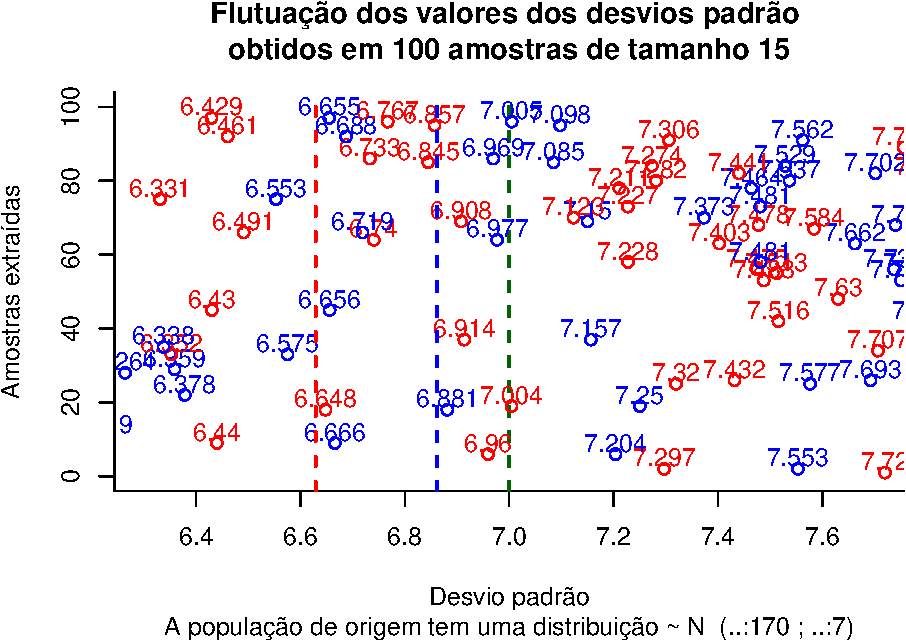
\includegraphics[width=0.8\linewidth]{apostila_files/figure-latex/unnamed-chunk-37-1} 

}

\caption{Diferentes formas na distribuição dos dados}\label{fig:unnamed-chunk-37}
\end{figure}

\hfill\break

De modo assemelhado, o histograma pode denotar uma forma mais \emph{plana} ou menos \emph{aguda}, onde um \emph{cume} mostra-se mais destacado.

\hfill\break

Nesse aspecto da forma, uma variável com distribuição Gaussiana apresentaria uma curva a que denominamos \emph{mesocúrtica}. Distribuições com um aspecto mais plano são denominadas de \emph{platicúrticas} e as com um cume agudo são denominadas \emph{leptocúrticas}.

\hfill\break

A curtose é uma medida da agudeza da distribuição dos dados em relação à distribuição Gaussiana.

\hfill\break

\begin{figure}

{\centering 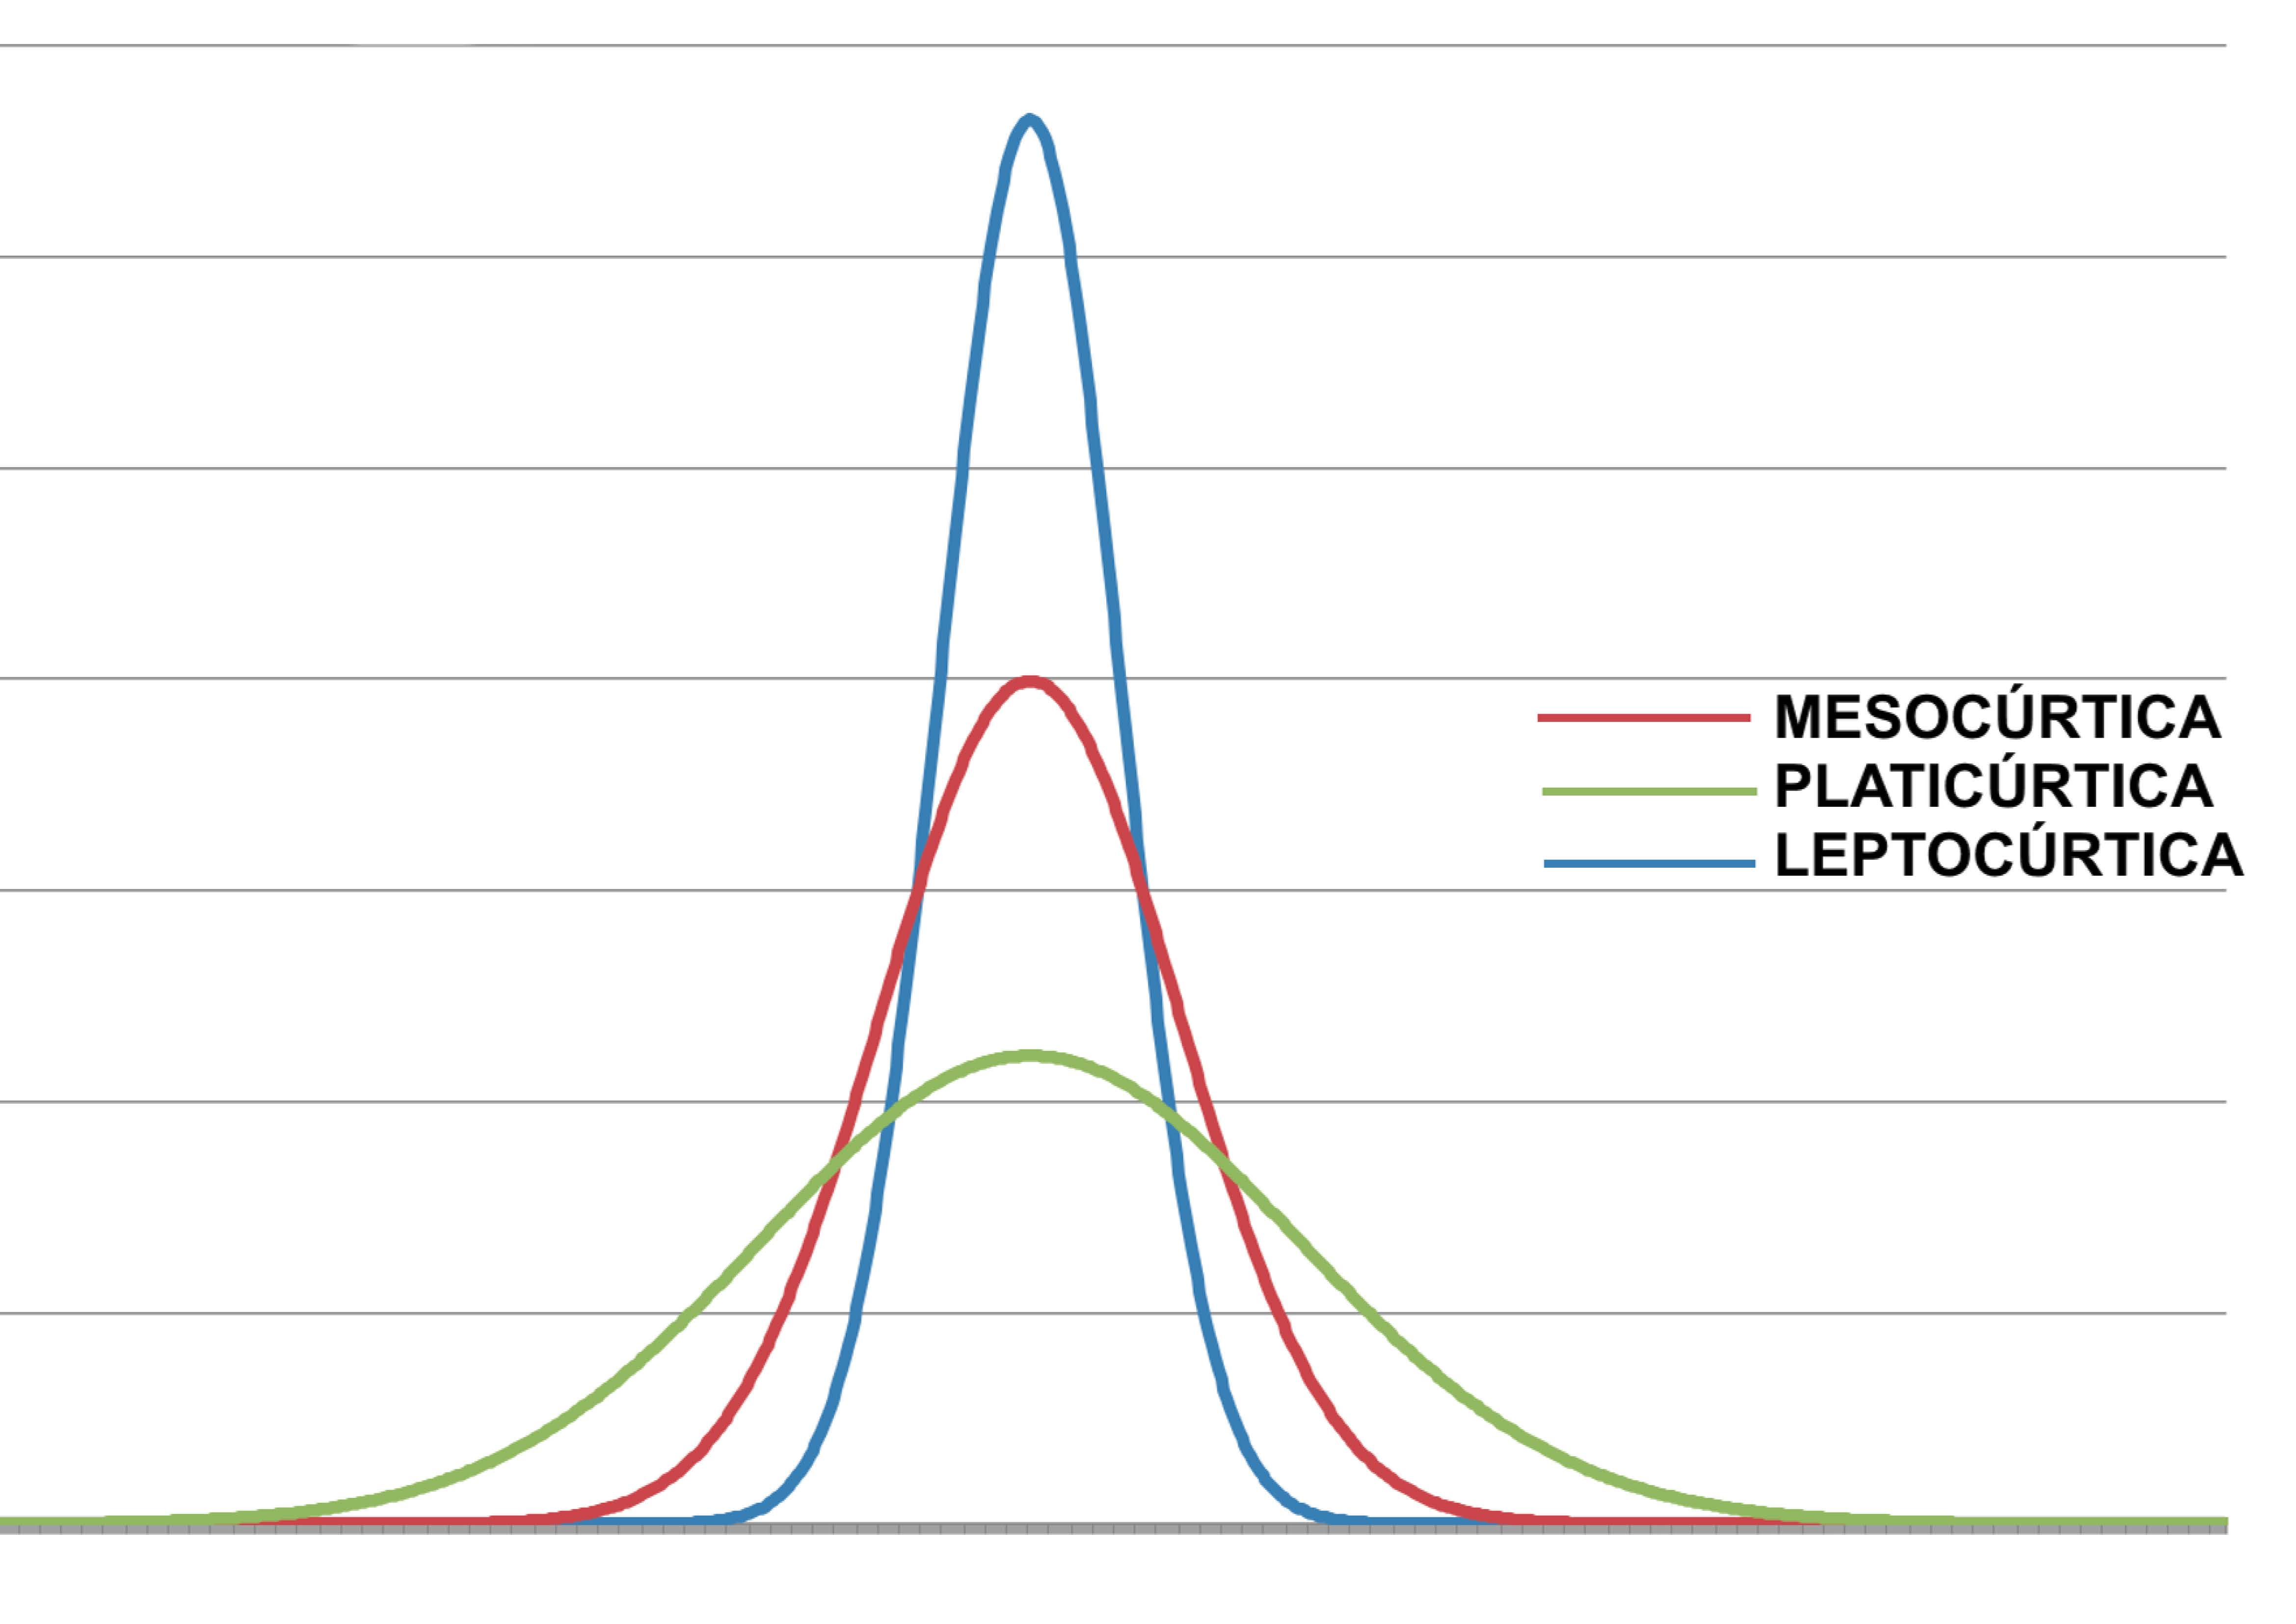
\includegraphics[width=0.8\linewidth]{images3/curtose} 

}

\caption{Diferentes aspectos de uma distribuição quanto à sua inclinação}\label{fig:unnamed-chunk-38}
\end{figure}

\hfill\break

Essas possíveis variações na forma de uma distribuição podem ser numericamente quantificadas através dos \emph{coeficientes de assimetria e curtose}.

\hfill\break

Uma das medidas do coeficiente de assimetria é através do \emph{primeiro ou segundo coeficientes de Pearson}, dados pelas seguintes relações:

\hfill\break

\begin{itemize}
\tightlist
\item
  Primeiro coeficiente de assimetria de Pearson: \(AS= \frac{ \stackrel{-}{x} - M_{o} }{ s }\)
\item
  Segundo coeficiente de assimetria de Pearson: \(AS = \frac{ 3 ( \stackrel{-}{x} - M_{d}) } { s }\)
\end{itemize}

\hfill\break

Onde:

\hfill\break

\begin{itemize}
\tightlist
\item
  \(\stackrel{-}{x}\) é a média;
\item
  \(M_{o}\) é a moda;
\item
  \(S\) é o desvio padrão; e,
\item
  \(M_{d}\) é a mediana.
\end{itemize}

\hfill\break

A \emph{assimetria} é classificada do modo seguinte:

\hfill\break

\begin{itemize}
\tightlist
\item
  AS=0: distribuição simétrica;
\item
  AS\textless0: distribuição com assimetria negativa; e,
\item
  AS\textgreater0: distribuição com assimetria positiva.
\end{itemize}

\hfill\break

Uma das medidas do coeficiente de curtose é através da seguinte relação entre \emph{quartis} e \emph{percentis}:

\hfill\break

\[
K = \frac{\frac{Q_{3} - Q_{1}}{2}   }   {P_{90} - P_{10}} 
\]

\hfill\break

Onde:

\hfill\break

\begin{itemize}
\tightlist
\item
  \(Q_{3}\) = \(3^{o}\) quartil;
\item
  \(Q_{1}\) = \(1^{o}\) quartil;
\item
  \(P_{90}\) = \(90^{o}\) percentil; e,
\item
  \(P_{10}\) = \(10^{o}\) percentil.
\end{itemize}

\hfill\break

O \emph{coeficiente de curtose} é classificado do modo seguinte:

\hfill\break

\begin{itemize}
\tightlist
\item
  k = 0; 263: distribuição mesocúrtica;
\item
  k \textless{} 0; 263: distribuição leptocúrtica; e,
\item
  k \textgreater{} 0; 263: distribuição platicúrtica.
\end{itemize}

\hypertarget{apresentauxe7uxe3o-tabular-de-dados}{%
\section{Apresentação tabular de dados}\label{apresentauxe7uxe3o-tabular-de-dados}}

\hfill\break

As sínteses numéricas expostas condensam ao máximo a informação trazida pelos dados na forma de estatísticas associadas à:

\hfill\break

\begin{itemize}
\tightlist
\item
  posição: média, moda, mediana;
\item
  dispersão: amplitude total dos dados, variância (esvio padrão), coeficiente de variação;
\item
  separatrizes (repartição): como por exemplo os quartis (\(Q_{1}\); \(Q_{2}\)/mediana e \(Q_{3}\)).
\end{itemize}

\hfill\break

A correta exposição dos dados na forma de tabelas e gráficos auxilia o entendimento de muitas outras características relacionadas aos dados trabalhados por parte do leitor com grande riqueza visual.

\hfill\break

Ao se lidar com grandes conjuntos de dados a visualização da informação contida nos dados fica comprometida se eles forem simplesmente apresentados como uma listagem, mesmo que depurados de eventuais inconsistências e ordenados como a lista abaixo:

\hfill\break

\begin{Shaded}
\begin{Highlighting}[]
\FunctionTok{sort}\NormalTok{(alturas)}
\end{Highlighting}
\end{Shaded}

\begin{verbatim}
##  [1] 1.41 1.44 1.47 1.54 1.55 1.56 1.56 1.56 1.57 1.58 1.58 1.61 1.62 1.62 1.63
## [16] 1.64 1.64 1.65 1.65 1.65 1.65 1.66 1.66 1.66 1.66 1.66 1.67 1.67 1.67 1.67
## [31] 1.68 1.68 1.68 1.69 1.71 1.71 1.72 1.72 1.73 1.73 1.73 1.73 1.73 1.74 1.75
## [46] 1.76 1.76 1.77 1.78 1.78 1.79 1.82 1.83 1.83 1.84 1.85 1.86 1.93 1.95 2.00
\end{verbatim}

\hfill\break

Um dos modos de se lidar com isso é condensando a informação dos dados brutos em tabelas.

\hfill\break

Uma tabela é uma forma não discursiva de apresentar informações nas quais o dado numérico se destaca como informação central. Uma tabela se diferencia de um quadro por este ter todos os seus campos delimitados por linhas e conter apenas informações de natureza qualitativa.

\hfill\break

Uma tabela deve conter algumas \textbf{informações essenciais}, fora daquela estritamente relacionada aos dados, para que a compreensão do leitor acerca dos dados expostos seja a mais imediata possível:

\hfill\break

\begin{itemize}
\tightlist
\item
  título que explique o que a tabela contém, local, data;
\item
  cabeçalho nas colunas e linhas com a explicação, ainda que resumis, a que se referem as quantidades expostas no corpo;
\item
  corpo formado pelos dados referentes às variáveis;
\item
  fonte dos dados;
\item
  uniformidade no número de casas decimais apresentadas no corpo;
\item
  todas as casas devem apresentar valores ou símbolos que expliquem a ausência da informação (NI, NE, ou 0-zero).
\end{itemize}

\hfill\break

Trabalhos de natureza acadêmica ou científica deveriam obrigatoriamente seguir, quando publicados no Brasil, a norma vigente publicada pela ABNT: Associação Brasileira de Normas Técnicas e algumas punlicações do IBGE: Instituto Brasileiro de Geografia e Estatística (como em \href{https://biblioteca.ibge.gov.br/visualizacao/livros/liv23907.pdf}{link}).

\hfill\break

Observa-se frequentemente, todavia, que as publicações seguem normas particulares das instituições de ensino (para trabalhos de conclusão de curso, monografias, dissertações e teses) ou das editoras (artigos), muitas vezes mescladas com recomendações da ABNT. Na Universidade Estadual de Londrina o portal da biblioteca possui uma ligação para a seção ``Normas para trabalhos'' (\href{https://sites.uel.br/bibliotecas/}{link}).

\hfill\break

\hypertarget{apresentauxe7uxe3o-tabular-de-dados-qualitativos}{%
\subsection{Apresentação tabular de dados qualitativos}\label{apresentauxe7uxe3o-tabular-de-dados-qualitativos}}

\hfill\break

Para alguns tipos de dados, a apresentação tabular é bastante imediata.

\hfill\break

Admita que tenha sido realizada uma pesquisa junto a um terminal de desembarque internacional em algum aeroporto sobre o continente de procedência do passageiro, num determinado período de um certo dia, tendo sido anotados os seguintes valores: AM, AM, A, A, A, AM, EU, EU, EU, EU, AM, AS, AS, AS, OC, AS, EU, AM, onde os continente anotados são assim identificados: americano (AM); africano (A), europeu (EU); asiático (AS) e da oceania (OC). Uma tabela para a apresentação dos resultados poderia ser:

\hfill\break

\begin{table}[h]
\centering
\caption{Desembarques no terminal internacional A em Cumbica (SP, Brasil) \\\hspace{\textwidth} (10/10/2021: 8 h 00min às 12 h 00 min)}
\begin{tabular}{|l|l|}
\hline
Continente de procedência   &  Desembarques  \\
\hline
América & 5 \\                                |
África  & 3 \\                           
Europa  & 5 \\                          
Ásia    & 4 \\                          
Oceania & 1 \\                        
\hline
Total  & 18 \\   
\hline
\end{tabular}
\end{table} 

\hfill\break

A partir desse resumo, poderíamos eleborar a apresentação gráfica desses dados na forma de um \emph{Gráfico de colunas} ou um \emph{Gráfico de setores}.

\hfill\break

\begin{Shaded}
\begin{Highlighting}[]
\NormalTok{desembarque}\OtherTok{=}\FunctionTok{c}\NormalTok{(}\StringTok{\textquotesingle{}AM\textquotesingle{}}\NormalTok{,}\StringTok{\textquotesingle{}AM\textquotesingle{}}\NormalTok{,}\StringTok{\textquotesingle{}A\textquotesingle{}}\NormalTok{,}\StringTok{\textquotesingle{}A\textquotesingle{}}\NormalTok{,}\StringTok{\textquotesingle{}A\textquotesingle{}}\NormalTok{,}\StringTok{\textquotesingle{}AM\textquotesingle{}}\NormalTok{,}\StringTok{\textquotesingle{}EU\textquotesingle{}}\NormalTok{,}\StringTok{\textquotesingle{}EU\textquotesingle{}}\NormalTok{,}\StringTok{\textquotesingle{}EU\textquotesingle{}}\NormalTok{,}\StringTok{\textquotesingle{}EU\textquotesingle{}}\NormalTok{,}\StringTok{\textquotesingle{}AM\textquotesingle{}}\NormalTok{,}\StringTok{\textquotesingle{}AS\textquotesingle{}}\NormalTok{,}\StringTok{\textquotesingle{}AS\textquotesingle{}}\NormalTok{,}\StringTok{\textquotesingle{}AS\textquotesingle{}}\NormalTok{,}\StringTok{\textquotesingle{}OC\textquotesingle{}}\NormalTok{,}\StringTok{\textquotesingle{}AS\textquotesingle{}}\NormalTok{,}\StringTok{\textquotesingle{}EU\textquotesingle{}}\NormalTok{,}\StringTok{\textquotesingle{}AM\textquotesingle{}}\NormalTok{)}
\NormalTok{tab\_desembarque}\OtherTok{=}\FunctionTok{table}\NormalTok{(desembarque)}

\FunctionTok{barplot}\NormalTok{(tab\_desembarque,}
        \AttributeTok{main=}\StringTok{"Fig. 01: Desembarques no terminal internacional A em Cumbica }\SpecialCharTok{\textbackslash{}n}\StringTok{(10/10/2021: 8 h 00min às 12 h 00 min)"}\NormalTok{,}
        \AttributeTok{sub=} \StringTok{"Continente de procedência: América: AM; África: A; Europa: EU; Ásia: AS; Oceania: OC }\SpecialCharTok{\textbackslash{}n}\StringTok{fonte: próprio autor"}\NormalTok{,}
        \AttributeTok{xlab=}\StringTok{""}\NormalTok{,}
        \AttributeTok{ylab=}\StringTok{"Quantidade observada (un)"}\NormalTok{,}
        \AttributeTok{ylim=}\FunctionTok{c}\NormalTok{(}\DecValTok{0}\NormalTok{,}\DecValTok{6}\NormalTok{),}
        \AttributeTok{col=}\StringTok{"blue"}\NormalTok{,}
        \AttributeTok{las=}\DecValTok{0}\NormalTok{, }
        \AttributeTok{hor=}\StringTok{"FALSE"}\NormalTok{)}
\end{Highlighting}
\end{Shaded}

\begin{figure}
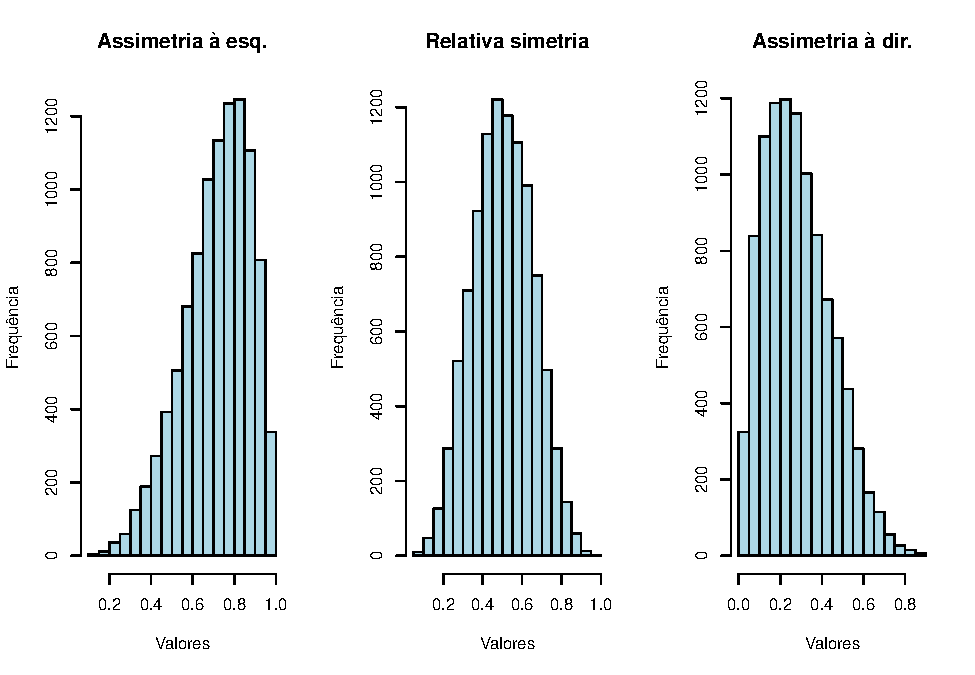
\includegraphics[width=0.8\linewidth]{apostila_files/figure-latex/unnamed-chunk-41-1} \caption{Gráfico de barras dos dados observados no terminal de desembarque internacional do aeroporto}\label{fig:unnamed-chunk-41}
\end{figure}

\hfill\break

ou ainda assim:

\hfill\break

\begin{Shaded}
\begin{Highlighting}[]
\FunctionTok{library}\NormalTok{(scales)}
\FunctionTok{library}\NormalTok{(ggplot2)}

\NormalTok{desembarques\_classes}\OtherTok{=}\FunctionTok{data.frame}\NormalTok{(}
  \AttributeTok{group =} \FunctionTok{c}\NormalTok{(}\StringTok{"América"}\NormalTok{,}\StringTok{"África"}\NormalTok{,}\StringTok{"Europa"}\NormalTok{,}\StringTok{"Ásia"}\NormalTok{,}\StringTok{"Oceania"}\NormalTok{),}
  \AttributeTok{value =} \FunctionTok{c}\NormalTok{(}\DecValTok{5}\NormalTok{,}\DecValTok{3}\NormalTok{,}\DecValTok{5}\NormalTok{,}\DecValTok{4}\NormalTok{,}\DecValTok{1}\NormalTok{))}


\NormalTok{blank\_theme}\OtherTok{=}\FunctionTok{theme\_minimal}\NormalTok{()}\SpecialCharTok{+}
  \FunctionTok{theme}\NormalTok{(}
    \AttributeTok{axis.title.x =} \FunctionTok{element\_blank}\NormalTok{(),}
    \AttributeTok{axis.title.y =} \FunctionTok{element\_blank}\NormalTok{(),}
    \AttributeTok{panel.border =} \FunctionTok{element\_blank}\NormalTok{(),}
    \AttributeTok{panel.grid=}\FunctionTok{element\_blank}\NormalTok{(),}
    \AttributeTok{axis.ticks =} \FunctionTok{element\_blank}\NormalTok{(),}
    \AttributeTok{plot.title=}\FunctionTok{element\_text}\NormalTok{(}\AttributeTok{size=}\DecValTok{14}\NormalTok{, }\AttributeTok{face=}\StringTok{"bold"}\NormalTok{)}
\NormalTok{  )}

\FunctionTok{ggplot}\NormalTok{(desembarques\_classes, }\FunctionTok{aes}\NormalTok{(}\AttributeTok{x=}\StringTok{""}\NormalTok{, }\AttributeTok{y=}\NormalTok{value, }\AttributeTok{fill=}\NormalTok{group)) }\SpecialCharTok{+}
\NormalTok{  blank\_theme }\SpecialCharTok{+}
  \FunctionTok{scale\_fill\_brewer}\NormalTok{(}\StringTok{"Blues"}\NormalTok{)}\SpecialCharTok{+}
  \FunctionTok{labs}\NormalTok{(}\AttributeTok{title=}\StringTok{"Fig. 01: Desembarques no terminal internacional A em Cumbica"}\NormalTok{, }
          \AttributeTok{subtitle=}\StringTok{"(10/10/2021: 8 h 00min às 12 h 00 min)"}\NormalTok{,}
           \AttributeTok{caption =} \StringTok{"Fonte: próprio autor"}\NormalTok{) }\SpecialCharTok{+}
  \FunctionTok{theme}\NormalTok{(}\AttributeTok{axis.text.x=}\FunctionTok{element\_blank}\NormalTok{()) }\SpecialCharTok{+}
  \FunctionTok{geom\_bar}\NormalTok{(}\AttributeTok{width =} \DecValTok{1}\NormalTok{, }\AttributeTok{stat =} \StringTok{"identity"}\NormalTok{) }\SpecialCharTok{+}
  \FunctionTok{coord\_polar}\NormalTok{(}\StringTok{"y"}\NormalTok{, }\AttributeTok{start=}\DecValTok{0}\NormalTok{) }\SpecialCharTok{+}
  \FunctionTok{geom\_text}\NormalTok{(}\FunctionTok{aes}\NormalTok{(}\AttributeTok{y =}\NormalTok{ value}\SpecialCharTok{/}\DecValTok{2} \SpecialCharTok{+} \FunctionTok{c}\NormalTok{(}\DecValTok{0}\NormalTok{, }\FunctionTok{cumsum}\NormalTok{(value)[}\SpecialCharTok{{-}}\FunctionTok{length}\NormalTok{(value)]),}
                \AttributeTok{label =} \FunctionTok{percent}\NormalTok{(value}\SpecialCharTok{/}\DecValTok{18}\NormalTok{ )), }\AttributeTok{size=}\DecValTok{5}\NormalTok{)}\SpecialCharTok{+}
  \FunctionTok{guides}\NormalTok{(}\AttributeTok{fill =} \FunctionTok{guide\_legend}\NormalTok{(}\AttributeTok{title =} \StringTok{"Legenda"}\NormalTok{,}
                             \AttributeTok{label.position =} \StringTok{"right"}\NormalTok{,}
                             \AttributeTok{title.position =} \StringTok{"top"}\NormalTok{, }\AttributeTok{title.vjust =} \DecValTok{1}\NormalTok{)) }
\end{Highlighting}
\end{Shaded}

\begin{figure}
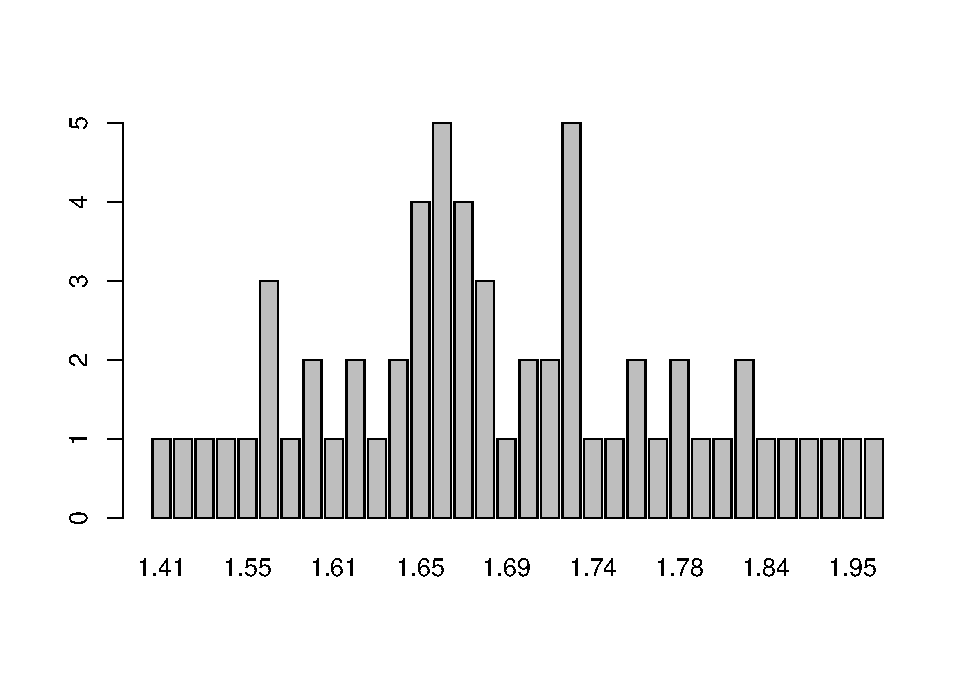
\includegraphics[width=0.8\linewidth]{apostila_files/figure-latex/unnamed-chunk-42-1} \caption{Gráfico de setores dos desembarques}\label{fig:unnamed-chunk-42}
\end{figure}

\hfill\break

Outro exemplo de apresentação tabular onde são apresentadas as proporções observadas de cada nível da variável estudada (``tipo de família'', com quatro níveis diferentes), de um levantamento amostral feito pela Agência do Censo dos Estados Unidos em 2005.

\hfill\break

\begin{table}[h]
\centering
\caption{Estrutura domiciliar dos Estados Unidos}
\begin{tabular}{|l|l|l|l|}
\hline
Estrutura domiciliar   & Número (milhões)  & Freq. rel.  & Freq. rel.  (\%) \\
\hline
Casal com filhos       & 24,1             & 0,22       & 22               \\
Casal sem filhos       & 31,1             & 0,28       & 28               \\
Solteiro, sem parceiro & 19,1             & 0,17       & 17               \\
Morando sozinho        & 30,1             & 0,27       & 27               \\
Outros domicílios      & 6,7              & 0,06       & 6                \\
\hline
Total                  & 111.1            & 1,00       & 100\%            \\
\hline
\end{tabular}
\vspace{4pt}
Fonte: Censo dos EUA (2005)                                                
\end{table} 

\hfill\break

Igualmente, a apresentação gráfica desses dados pode feita, por exemplo, por um \emph{Gráfico de colunas} ou um \emph{Gráfico de setores}.

\hfill\break

\begin{Shaded}
\begin{Highlighting}[]
\FunctionTok{library}\NormalTok{(ggplot2)}
\NormalTok{dados}\OtherTok{=}\FunctionTok{data.frame}\NormalTok{(}\AttributeTok{tipo=}\FunctionTok{c}\NormalTok{(}\StringTok{"Casal com filhos"}\NormalTok{,}
                          \StringTok{"Casal sem filhos"}\NormalTok{,}
                          \StringTok{"Solteiro, s/parceiro"}\NormalTok{,}
                          \StringTok{"Morando sozinho"}\NormalTok{,}
                          \StringTok{"Outros domicíclios"}\NormalTok{),}
                 \AttributeTok{quant=}\FunctionTok{c}\NormalTok{(}\FloatTok{24.1}\NormalTok{, }\FloatTok{31.1}\NormalTok{, }
                       \FloatTok{19.1}\NormalTok{, }\FloatTok{30.1}\NormalTok{,}
                       \FloatTok{6.7}\NormalTok{))}

\FunctionTok{ggplot}\NormalTok{(dados, }\FunctionTok{aes}\NormalTok{(}\AttributeTok{x=}\NormalTok{tipo, }\AttributeTok{y=}\NormalTok{quant, }\AttributeTok{color=}\NormalTok{tipo)) }\SpecialCharTok{+}
\FunctionTok{geom\_bar}\NormalTok{(}\AttributeTok{stat=}\StringTok{"identity"}\NormalTok{, }\AttributeTok{position=}\FunctionTok{position\_dodge}\NormalTok{())}\SpecialCharTok{+}
\FunctionTok{ggtitle}\NormalTok{(}\StringTok{"Estrutura domiciliar dos Estados Unidos, 2005"}\NormalTok{) }\SpecialCharTok{+}
\FunctionTok{theme}\NormalTok{(}\AttributeTok{legend.position=}\StringTok{"bottom"}\NormalTok{)}\SpecialCharTok{+}
\FunctionTok{geom\_text}\NormalTok{(}\FunctionTok{aes}\NormalTok{(}\AttributeTok{label=}\NormalTok{quant), }\AttributeTok{vjust=}\FloatTok{1.6}\NormalTok{, }\AttributeTok{color=}\StringTok{"white"}\NormalTok{, }\AttributeTok{position =} \FunctionTok{position\_dodge}\NormalTok{(}\FloatTok{0.9}\NormalTok{), }\AttributeTok{size=}\FloatTok{3.5}\NormalTok{)}\SpecialCharTok{+}
\FunctionTok{scale\_fill\_brewer}\NormalTok{(}\AttributeTok{palette=}\StringTok{"Paired"}\NormalTok{)}\SpecialCharTok{+}
\FunctionTok{theme\_minimal}\NormalTok{()}\SpecialCharTok{+}
\FunctionTok{xlab}\NormalTok{(}\StringTok{""}\NormalTok{)  }\SpecialCharTok{+}
\FunctionTok{ylab}\NormalTok{(}\StringTok{"Frequência absoluta observada (milhões)"}\NormalTok{)}\SpecialCharTok{+}
\FunctionTok{labs}\NormalTok{(}\AttributeTok{colour =} \StringTok{"Tipos de domicílios"}\NormalTok{) }
\end{Highlighting}
\end{Shaded}

\begin{figure}
\centering
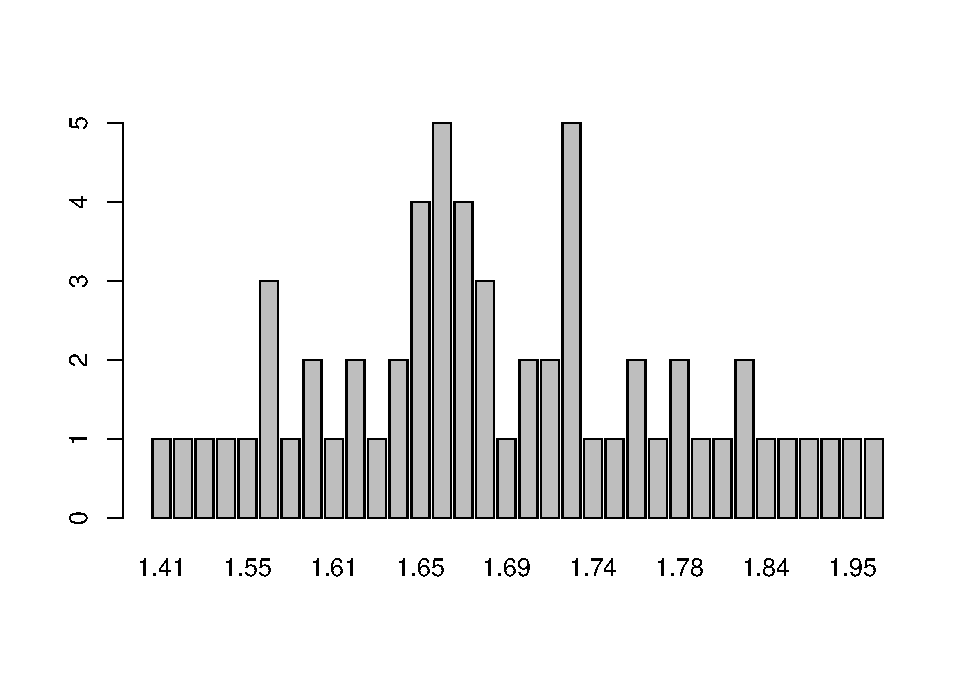
\includegraphics{apostila_files/figure-latex/unnamed-chunk-44-1.pdf}
\caption{\label{fig:unnamed-chunk-44}Gráfico de barras}
\end{figure}

\hfill\break

\begin{Shaded}
\begin{Highlighting}[]
\FunctionTok{library}\NormalTok{(ggplot2)}
\FunctionTok{library}\NormalTok{(scales)}

\NormalTok{blank\_theme}\OtherTok{=}\FunctionTok{theme\_minimal}\NormalTok{()}\SpecialCharTok{+}
  \FunctionTok{theme}\NormalTok{(}
    \AttributeTok{axis.title.x =} \FunctionTok{element\_blank}\NormalTok{(),}
    \AttributeTok{axis.title.y =} \FunctionTok{element\_blank}\NormalTok{(),}
    \AttributeTok{panel.border =} \FunctionTok{element\_blank}\NormalTok{(),}
    \AttributeTok{panel.grid=}\FunctionTok{element\_blank}\NormalTok{(),}
    \AttributeTok{axis.ticks =} \FunctionTok{element\_blank}\NormalTok{(),}
    \AttributeTok{plot.title=}\FunctionTok{element\_text}\NormalTok{(}\AttributeTok{size=}\DecValTok{14}\NormalTok{, }\AttributeTok{face=}\StringTok{"bold"}\NormalTok{)}
\NormalTok{  )}

\NormalTok{bp}\OtherTok{=}\FunctionTok{ggplot}\NormalTok{(dados, }\FunctionTok{aes}\NormalTok{(}\AttributeTok{x=}\StringTok{""}\NormalTok{, }\AttributeTok{y=}\NormalTok{quant, }\AttributeTok{fill=}\NormalTok{tipo))}\SpecialCharTok{+}
  \FunctionTok{geom\_bar}\NormalTok{(}\AttributeTok{width =} \DecValTok{1}\NormalTok{, }\AttributeTok{stat =} \StringTok{"identity"}\NormalTok{)}
\NormalTok{pie}\OtherTok{=}\NormalTok{bp }\SpecialCharTok{+} \FunctionTok{coord\_polar}\NormalTok{(}\StringTok{"y"}\NormalTok{, }\AttributeTok{start=}\DecValTok{0}\NormalTok{)}
\NormalTok{pie }\SpecialCharTok{+} 
  \FunctionTok{scale\_fill\_brewer}\NormalTok{(}\StringTok{"Blues"}\NormalTok{)}\SpecialCharTok{+}
\NormalTok{  blank\_theme }\SpecialCharTok{+}
  \FunctionTok{theme}\NormalTok{(}\AttributeTok{axis.text.x=}\FunctionTok{element\_blank}\NormalTok{()) }\SpecialCharTok{+}
  \FunctionTok{geom\_text}\NormalTok{(}\FunctionTok{aes}\NormalTok{(}\AttributeTok{x =}  \FloatTok{1.2}\NormalTok{,}\AttributeTok{label =}\NormalTok{ quant), }\AttributeTok{position =} \FunctionTok{position\_stack}\NormalTok{(}\AttributeTok{vjust =} \FloatTok{0.5}\NormalTok{)) }\SpecialCharTok{+}
  \FunctionTok{ggtitle}\NormalTok{(}\StringTok{"Estrutura domiciliar dos Estados Unidos, 2005"}\NormalTok{) }\SpecialCharTok{+}
  \FunctionTok{theme}\NormalTok{(}\AttributeTok{legend.position =} \StringTok{"right"}\NormalTok{, }\AttributeTok{legend.justification =} \StringTok{"center"}\NormalTok{, }\AttributeTok{legend.direction =} \StringTok{"vertical"}\NormalTok{,}
        \AttributeTok{legend.spacing.x =} \FunctionTok{unit}\NormalTok{(}\FloatTok{0.5}\NormalTok{, }\StringTok{\textquotesingle{}cm\textquotesingle{}}\NormalTok{),}\AttributeTok{legend.spacing.y =} \FunctionTok{unit}\NormalTok{(}\FloatTok{0.5}\NormalTok{, }\StringTok{\textquotesingle{}cm\textquotesingle{}}\NormalTok{))}\SpecialCharTok{+}
  \FunctionTok{guides}\NormalTok{(}\AttributeTok{fill =} \FunctionTok{guide\_legend}\NormalTok{(}\AttributeTok{title =} \StringTok{"Tipos de domicílios"}\NormalTok{,}
                             \AttributeTok{label.position =} \StringTok{"right"}\NormalTok{,}
                             \AttributeTok{title.position =} \StringTok{"top"}\NormalTok{, }\AttributeTok{title.vjust =} \DecValTok{1}\NormalTok{)) }
\end{Highlighting}
\end{Shaded}

\begin{figure}
\centering
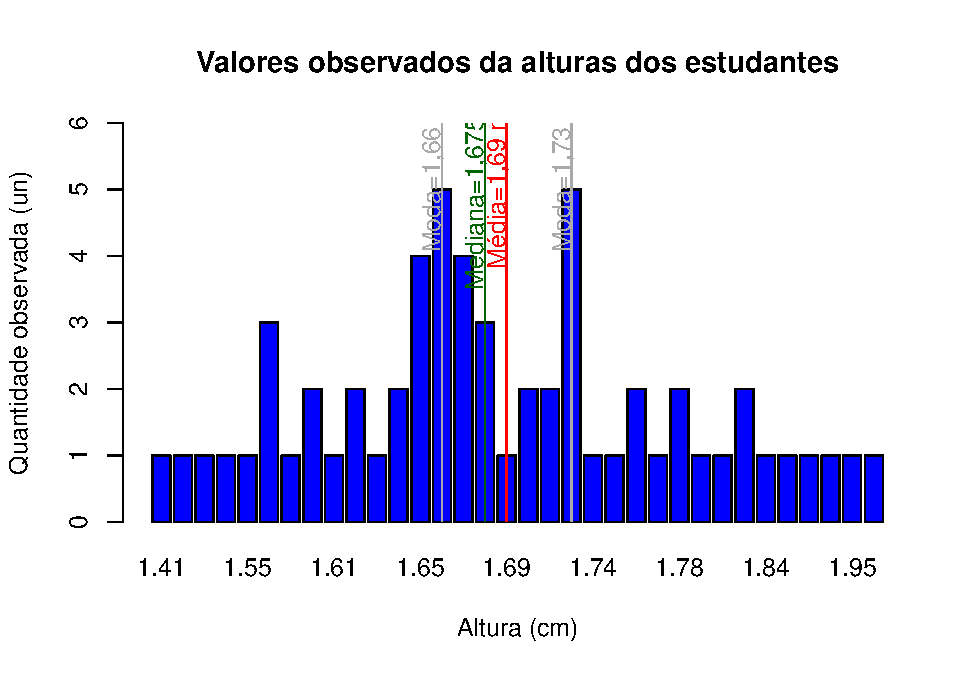
\includegraphics{apostila_files/figure-latex/unnamed-chunk-45-1.pdf}
\caption{\label{fig:unnamed-chunk-45}Gráfico de setores}
\end{figure}

\hfill\break

Outros tipos de dados são provenientes de pesquisas que tẽm por base respostas de natureza binária como, por exemplo:

\hfill\break

\begin{itemize}
\tightlist
\item
  sim ou não;
\item
  gosto ou não gosto;
\item
  voto em ``A'' ou voto em ``B''; ou,
\item
  concordo ou não concordo.
\end{itemize}

\hfill\break

Como resultado final, são obtidas contagens que expressam as frequências absolutas observadas para cada uma das variáveis (ou seus níveis) como na apresentação tabular de dados qualitativos por \emph{Tabelas de Contingência}.

\hfill\break

As \emph{tabelas de contingência} são usadas para associar duas ou mais variáveis qualitativas (ou seus níveis) às contagens das respostas obtidas, na forma das frequências absoluta e relativa observadas em cada uma dessas variáveis (ou seus níveis).

\hfill\break

O uso desse tipo de tabela é comum quando se pretende investigar se as variáveis estudadas têm alguma associação por meio de testes não paramétricos. Esse tipo de apresentação facilita a extração de informações relacionadas às probabilidades marginais ou condicionadas de cada uma variáveis ou seus níveis.

\hfill\break

\begin{table}[h]
\centering
\caption{Inclinação partidária (frequências absolutas)}
\begin{tabular}{|l|l|l|l|}
\hline
Estrutura domiciliar    & Democrata          & Republicano &  Totais        \\
\hline
Casal com filho(s)    & 762                & 468         & 1230            \\
Casal sem filhos      & 484                & 477         & 961             \\
\hline
Totais                & 1246               & 945         & 2191           \\
\hline
\end{tabular}
\end{table} 

\hfill\break

A partir das contagens obtidas na pesquisa, uma tabela com frequências relativas pode ser construída:

\hfill\break

\begin{table}[h]
\centering
\caption{Inclinação partidária (frequências relativas)}
\begin{tabular}{|l|l|l|l|}
\hline
Estrutura domiciliar    & Democrata (\%)          & Republicano (\%) &  Totais  (\%)      \\
\hline
Casal com filho(s)    & 34,78                & 21,36         & 56,14            \\
Casal sem filhos      & 22,09                & 21,77         & 43,86             \\
\hline
Totais (\%)               & 56,87               & 43,13         & 100           \\
\hline
\end{tabular}
\end{table} 

\begin{verbatim}
                                                               |
\end{verbatim}

As representações gráficas são análogas às mostradas no exemplo anterior.

\hfill\break

\hypertarget{apresentauxe7uxe3o-tabular-de-dados-quantitativos}{%
\subsection{Apresentação tabular de dados quantitativos}\label{apresentauxe7uxe3o-tabular-de-dados-quantitativos}}

\hfill\break

Todavia, para grandes quatidades de observações de dados quantitativos, a apresentação na forma de tabelas deve ser precedida do agrupamento dos valores observados em classes. O procedimento estatístico de agrupar os dados em \emph{classes} ou \emph{categorias} envolve construir uma \emph{tabela de distribuição de frequências}.

\hfill\break

Uma \emph{tabela de distribuição de frequências} associa cada \emph{classe} (intervalo) de valores da variável estudada ao número de ocorrências observadas. Como \emph{regra prática}, a repartição dos dados brutos em classes deve sempre observar para que não haja um número excessivo de classes (diminuição da finalidade de resumir os dados, criação de classes sem nenhuma observação) nem tampouco poucas (que não possibilitem a visualização da distribuição e promovam perda da informação original).

\hfill\break

A construção de uma \emph{distribuição de frequências} consiste essencialmente em:

\hfill\break

\begin{itemize}
\tightlist
\item
  escolher as \emph{classes} ou \emph{intervalos} (dados quantitativos) ou \emph{categorias} (dados qualitativos);
\item
  separar ou enquadrar os dados nessas \emph{classes} ou \emph{categorias}; e,
\item
  contar o número de dados de cada \emph{classe} ou \emph{categoria}.
\end{itemize}

\hfill\break

A literatura propõe vários modos para se determinar o número \emph{k} de classes:

\hfill\break

\begin{longtable}[]{@{}
  >{\raggedright\arraybackslash}p{(\columnwidth - 4\tabcolsep) * \real{0.3636}}
  >{\raggedright\arraybackslash}p{(\columnwidth - 4\tabcolsep) * \real{0.3377}}
  >{\raggedright\arraybackslash}p{(\columnwidth - 4\tabcolsep) * \real{0.2987}}@{}}
\toprule\noalign{}
\begin{minipage}[b]{\linewidth}\raggedright
Crítério
\end{minipage} & \begin{minipage}[b]{\linewidth}\raggedright
Tamanho da amostra (\emph{n})
\end{minipage} & \begin{minipage}[b]{\linewidth}\raggedright
Fórmula
\end{minipage} \\
\midrule\noalign{}
\endhead
\bottomrule\noalign{}
\endlastfoot
Raiz quadrada & 25 \(\leq\) n \(\leq\) 220 & k=\(\sqrt{n}\) \\
Herbert \textbf{Sturges} & 135 \(\leq\) 572237 & k=1+3,3log(n)\(^{(1)}\) \\
Giuseppe \textbf{Milone} & 20 \(\leq 36315\) & k=-1+2ln(n) \(^{(2)}\) \\
\end{longtable}

\begin{itemize}
\tightlist
\item
  \(^{(1)}\): logarítmo na base 10; e
\item
  \(^{(2)}\): logarítmo na base \emph{e}.
\end{itemize}

\hfill\break

Ao se escolher um número (\(k\)) de classes deve-se \textbf{ponderar} para que:

\hfill\break

\begin{itemize}
\tightlist
\item
  os intervalos das classes tenham, geralmente, a mesma amplitude (raramente se necessita dispor de classes com amplitudes diferentes);
\item
  os intervalos, a faixa de variação que vai do limite inferior da \textbf{primeira classe} ao limite superior da **última classe*, devem conter todos os valores possíveis da variável;
\item
  cada valor observado deve pertencer \textbf{apenas a uma classe};
\item
  nenhuma classe deverá estar vazia (sem observação alguma);\\
\item
  não adotar um número muito elevado de classes de modo que cada classe possua poucas observações (ou mesmo nenhuma); e,
\item
  não adotar um número muito reduzido de classes de modo a esconder a variabilidade dos dados ao se reunir todas as observações em poucas faixas de valores;
\item
  alguns autores recomendam um número mínimo de 5 classes e um máximo de 15.
\end{itemize}

\hfill\break

Em nosso exemplo das alturas dos estudantes, a determinação do número de classes pelo critério da \emph{raiz quadrada} ( \emph{n}=60) sugere 8 classes (pelo critérios de Sturges \(k=6,86 \sim 7\) e de Giuseppe Milone \(k=8,18 \sim 9)\)):

\hfill\break

\begin{align*}
k & =\sqrt{n} \\
 & = 7,74 \\
\end{align*}

\hfill\break

Arredondar para \textbf{mais}: \(k=8\).

\hfill\break

A \emph{amplitude total} (\emph{C}) dos valores observados é a simples diferença entre o \emph{valor máximo} (2,00 m) e o \emph{valor mínimo} (1,41 m):

\hfill\break

\begin{align*}
C & =2,00-1,41 \\
 & =0,59 m 
\end{align*}

\hfill\break

A amplitude de cada uma das classes ( \emph{c}) será dada pelo quociente da \emph{amplitude total} ( \emph{C}) pelo \emph{número de classes} ( \emph{k}).\\

\begin{align*}
c & = \frac{C}{k} \\
  & = \frac{0,59}{8}\\ 
  & = 0,07375 m
\end{align*}

\hfill\break

Arredondar para \textbf{mais}: \(c=0,08 m\).

\hfill\break

As classes são então assim construídas:

\hfill\break

\begin{itemize}
\tightlist
\item
  Limite inferior da \(1^{a}\) classe (\(LI_{1}\)): valor mínimo observado; e,
\item
  Limite superior da \(1^{a}\) classe (\(LS_{1}\)): \(LI_{1}\) + c.~
\end{itemize}

\hfill\break

e assim sucessivamente atá a última classe.

\hfill\break

Símbolos gráficos para intervalos:

\hfill\break

\begin{itemize}
\tightlist
\item
  Os símbolos abaixo indicam que o valor situado à sua esquerda \textbf{está incluído} no intervalo e o da direita \textbf{não está}:
\end{itemize}

~

\[
\vdash \\
{\bullet}-{\circ}
\]

\hfill\break

\begin{itemize}
\tightlist
\item
  Os símbolos abaixo indicam que o valor situado à sua esquerda \textbf{não está} incluído no intervalo e o da direita **está incluído*:
\end{itemize}

\hfill\break

\[
\dashv  \\
{\circ}-{\bullet}
\]

\hfill\break

\begin{quote}
As tabelas que serão apresentadas a seguir estão sem os requisitos essenciais expostos anteriormente uma vez que o propósito é explicar a construção e cálculo dos valores de suas células.
\end{quote}

\hfill\break

Com \(c=0,08m\) as classes ficam assim estabelecidas, tendo-se como ponto de partida o valor mínimo observado: 1,41 m - 1,49 m; 1,49 m - 1,57 m; 1,57 m - 1,65 m; 1,65 m - 1,73 m; 1,73 m - 1,81 m; 1,81 m - 1,89 m; 1,89 m - 1,97m; 1,97 - 2,05 m.

\hfill\break

\{
\textcolor{blue}{ 1,41 ; 1,44 ; 1,47 ; 1,54 ; 1,55 ; 1,56 ; 1,56 ; 1,56 ;} 1,57 ; 1,58 ; 1,58 ; 1,61 ; 1,62 ; 1,62 ; 1,63 ; 1,64 ;1,64 ; \textcolor{blue}{ 1,65 ; 1,65 ; 1,65 ; 1,65 ; 1,66 ; 1,66 ; 1,66 ; 1,66 ; 1,66 ; 1,67 ; 1,67 ; 1,67 ; 1,67 ; 1,68 ; 1,68 ;1,68 ; 1,69 ; 1,71 ; 1,71 ; 1,72 ; 1,72 ;} 1,73 ; 1,73 ; 1,73 ; 1,73 ; 1,73 ; 1,74 ; 1,75 ; 1,76 ; 1,76 ; 1,77 ; 1,78 ; 1,78 ;1,79; \textcolor{blue}{1,82 ; 1,83 ; 1,83 ; 1,84 ; 1,85 ; 1,86  ;} 1,93 ; 1,95 ; \textcolor{blue}{2,00}\}

\hfill\break

A tabela de distribuição de frequências com 7 classes assume a forma:

\hfill\break

\begin{longtable}[]{@{}ll@{}}
\toprule\noalign{}
Classe & Frequência absoluta (\(f_{i}\)) \\
\midrule\noalign{}
\endhead
\bottomrule\noalign{}
\endlastfoot
1,41 m \(\vdash\) 1,57 m & 8 \\
1,57 m \(\vdash\) 1,65 m & 9 \\
1,65 m \(\vdash\) 1,73 m & 21 \\
1,73 m \(\vdash\) 1,81 m & 13 \\
1,81 m \(\vdash\) 1,89 m & 6 \\
1,89 m \(\vdash\) 1,97 m & 2 \\
1,97 m \(\vdash\) 2,05 m & 1 \\
Total & 60 \\
\end{longtable}

\hfill\break

Alternativamente, caso adotássemos como ponto de partida (um pouco abaixo do valor mínimo observado) o valor de 1,40 m, a distribuição das classes seria: 1,40 m - 1,48 m; 1,48 m - 1,56 m; 1,56 m - 1,64 m; 1,64 m - 1,72 m; 1,72 m - 1,80 m; 1,80 m - 1,88 m; 1,88 m - 2,06 m e, para facilitar a contagem das observações pertencentes a cada uma das classes ordenamos os dados:

\hfill\break

\{
\textcolor{blue}{1,41 ; 1,44 ; 1,47 ;}
1,54 ; 1,55 ;
\textcolor{blue}{1,56 ; 1,56 ; 1,56 ; 1,57 ; 1,58 ; 1,58 ; 1,61 ; 1,62 ; 1,62 ; 1,63 ;}
1,64 ;1,64 ; 1,65 ; 1,65 ; 1,65 ; 1,65 ; 1,66 ; 1,66 ; 1,66 ; 1,66 ; 1,66 ; 1,67 ; 1,67 ; 1,67 ; 1,67 ; 1,68 ; 1,68 ;1,68 ; 1,69 ; 1,71 ; 1,71 ;
\textcolor{blue}{1,72 ; 1,72 ; 1,73 ; 1,73 ; 1,73 ; 1,73 ; 1,73 ; 1,74 ; 1,75 ; 1,76 ; 1,76 ; 1,77 ;  1,78 ; 1,78 ;1,79;} 1,82 ; 1,83 ; 1,83 ; 1,84 ; 1,85 ; 1,86 ;
\textcolor{blue}{1,93 ; 1,95 ; 2,00;} \}

\hfill\break

A tabela de distribuição de frequências com 7 classes assume a forma:

\hfill\break

\begin{longtable}[]{@{}ll@{}}
\toprule\noalign{}
Classe & Frequência absoluta (\(f_{i}\)) \\
\midrule\noalign{}
\endhead
\bottomrule\noalign{}
\endlastfoot
1,40 m \(\vdash\) 1,48 m & 3 \\
1,48 m \(\vdash\) 1,56 m & 2 \\
1,56 m \(\vdash\) 1,64 m & 10 \\
1,64 m \(\vdash\) 1,72 m & 21 \\
1,72 m \(\vdash\) 1,80 m & 15 \\
1,80 m \(\vdash\) 1,88 m & 6 \\
1,88 m \(\vdash\) 2,06 m & 3 \\
Total & 60 \\
\end{longtable}

\hfill\break

Também podemos cogitar adotar alternativamente um intervalo de classe \(c=0,10\) m, com a primeira classe começando (um pouco abaixo do valor mínimo observado) na altura de 1,40 m; todavia, a última classe não iria contemplar o valor máximo observado (2,00 m) e necessitaíamos abrir mais uma classe apenas para incluí-lo.

\hfill\break

Mas começando-se no valor mínimo obseravado (1,41 m) estaríamos assegurando que o limite superior da última classe incluiria o valor máximo observado (2,00 m). Assim, essas seriam as classes sob uma amplitude de 0,10 m: 1,41 m - 1,51 m; 1,51 m - 1,61 m; 1,61 m - 1,71 m; 1,71 m - 1,81 m; 1,81 m - 1,91 m; 1,91 m - 2,01 m. O total de 6 classes (1,41 m a 2,01 m) cobre toda faixa de variação dos valores dos dados (de 1,41 m a 2,00 m ) e é de rápida assimilação pelo leitor.

\hfill\break

Ordenando-se os dados para facilitar a contagem das observações pertencentes a cada uma das classes:

\hfill\break

\{\textcolor{blue}{1,41 ; 1,44 ; 1,47 ;} 1,54 ; 1,55 ; 1,56 ; 1,56 ; 1,56 ; 1,57 ; 1,58 ; 1,58 ; \textcolor{blue}{1,61 ; 1,62 ; 1,62 ; 1,63 ; 1,64 ;1,64 ; 1,65 ; 1,65 ; 1,65 ; 1,65 ; 1,66 ; 1,66 ; 1,66 ; 1,66 ; 1,66 ; 1,67 ; 1,67 ; 1,67 ; 1,67 ; 1,68 ; 1,68 ;1,68 ; 1,69 ;} 1,71 ; 1,71 ; 1,72 ; 1,72 ; 1,73 ; 1,73 ; 1,73 ; 1,73 ; 1,73 ; 1,74 ; 1,75 ; 1,76 ; 1,76 ; 1,77 ; 1,78 ; 1,78 ; 1,79 ; \textcolor{blue}{1,82 ; 1,83 ; 1,83 ; 1,84 ; 1,85 ; 1,86 ;} 1,93 ; 1,95 ; 2,00\}

\hfill\break

A tabela de distribuição de frequências com 6 classes assume a forma:

\hfill\break

\begin{longtable}[]{@{}ll@{}}
\toprule\noalign{}
Classe & Frequência absoluta (\(f_{i}\)) \\
\midrule\noalign{}
\endhead
\bottomrule\noalign{}
\endlastfoot
1,41 m \(\vdash\) 1,51 m & 3 \\
1,51 m \(\vdash\) 1,61 m & 8 \\
1,61 m \(\vdash\) 1,71 m & 23 \\
1,71 m \(\vdash\) 1,81 m & 17 \\
1,81 m \(\vdash\) 1,91 m & 6 \\
1,91 m \(\vdash\) 2,01 m & 3 \\
Total & 60 \\
\end{longtable}

\hfill\break

\emph{Tabelas de distribuição de frequências} mais completas podem montadas agregando muitas informações adicionais em novas colunas, mediante simples operações aritméticas.

\hfill\break

Essas informações servem para tornar a visualização mais imediata e muitas delas são obtidas com operações matemáticas elementares:

\hfill\break

\begin{itemize}
\tightlist
\item
  Classe \emph{i}: é a simples identificação de cada classe;
\item
  Amplitude (\(\Delta_{i}\)) da classe \(i\): a diferença entre o valor do limite superior e o do inferior de cada classe;
\item
  Intervalo de valores da classe \(i\) (onde seu limite inferior \textbf{está contido} e o limite superior \textbf{não está contido});
\item
  Valor médio (\(\stackrel{-}{x}_{i}\)) de cada classe \(i\): o valor de seu \textbf{limite inferior} mais a metade da amplitude da classe;
\item
  Frequência absoluta (\(f_{i}\)) da classe \(i\): o número de observações contidas no intervalo da classe considerada;
\item
  Frequência relativa (\(fr_{i}= \frac{f_{i}}{N}\)) da classe \(i\) (ou frequência relativa percentual, se assim apresentada): o quociente do número de observações contidas no intervalo da classe (\(f_{i}\)) pelo número total de observações (\(N\));
\item
  Frequência acumulada (\(fac_{i}\)) da classe \(i\) (ou frequência acumulada percentual, se assim apresentada): o número de observações com medidas contidas na classe \(i\) e nas anteriores a ela;
\item
  Densidade absoluta (\(\delta_{i}=\frac{f_{i}}{\Delta_{i}}\)): o quociente do número de observações da classe (\(f_{i}\)) pela sua amplitude (\(\Delta_{i}\));
\item
  Densidade relativa \(\delta_{fr_{i}}=\frac{fr_{i}}{\Delta_{i}}\): o quociente da frequência relativa (\(fr_{i}\)) pela amplitude (\(\Delta_{i}\)) da classe.
\end{itemize}

\hfill\break

Vejo como exemplo as tabelas abaixo:

\hfill\break

\begin{longtable}[]{@{}
  >{\raggedright\arraybackslash}p{(\columnwidth - 14\tabcolsep) * \real{0.0597}}
  >{\raggedright\arraybackslash}p{(\columnwidth - 14\tabcolsep) * \real{0.1567}}
  >{\raggedright\arraybackslash}p{(\columnwidth - 14\tabcolsep) * \real{0.1866}}
  >{\raggedright\arraybackslash}p{(\columnwidth - 14\tabcolsep) * \real{0.0821}}
  >{\raggedright\arraybackslash}p{(\columnwidth - 14\tabcolsep) * \real{0.1194}}
  >{\raggedright\arraybackslash}p{(\columnwidth - 14\tabcolsep) * \real{0.1343}}
  >{\raggedright\arraybackslash}p{(\columnwidth - 14\tabcolsep) * \real{0.1269}}
  >{\raggedright\arraybackslash}p{(\columnwidth - 14\tabcolsep) * \real{0.1343}}@{}}
\toprule\noalign{}
\begin{minipage}[b]{\linewidth}\raggedright
Classe
\end{minipage} & \begin{minipage}[b]{\linewidth}\raggedright
Int. de valores
\end{minipage} & \begin{minipage}[b]{\linewidth}\raggedright
Alt. média
\end{minipage} & \begin{minipage}[b]{\linewidth}\raggedright
Freq. abs.
\end{minipage} & \begin{minipage}[b]{\linewidth}\raggedright
Freq. rel.
\end{minipage} & \begin{minipage}[b]{\linewidth}\raggedright
Freq. rel. (\%)
\end{minipage} & \begin{minipage}[b]{\linewidth}\raggedright
Freq. acumulada
\end{minipage} & \begin{minipage}[b]{\linewidth}\raggedright
Freq. acum. (\%)
\end{minipage} \\
\midrule\noalign{}
\endhead
\bottomrule\noalign{}
\endlastfoot
& & (\(\stackrel{-}{x}_{i}\)) & (\(f_{i}\)) & (\(fr_{i}\)) & (\(fr_{i}\%\)) & (\(fac_{i}\)) & (\(fac_{i}\%\)) \\
1 & 1,41 \(\vdash\) 1,51 & 1,46 & 3 & 0,05 & 5 & 3 & 5,00 \\
2 & 1,51 \(\vdash\) 1,61 & 1,56 & 8 & 0,13 & 13,33 & 11 & 18,33 \\
3 & 1,61 \(\vdash\) 1,71 & 1,66 & 23 & 0,38 & 38,33 & 34 & 56,66 \\
4 & 1,71 \(\vdash\) 1,81 & 1,76 & 17 & 0,28 & 28,34 & 51 & 85,00 \\
5 & 1,81 \(\vdash\) 1,91 & 1,86 & 6 & 0,10 & 10 & 57 & 95,00 \\
6 & 1,91 \(\vdash\) 2,01 & 1,96 & 3 & 0,05 & 5 & 60 & 100,00 \\
Totais & - & & 60 & 1,00 & 100,00 & - & - \\
\end{longtable}

\hfill\break

\begin{longtable}[]{@{}
  >{\raggedright\arraybackslash}p{(\columnwidth - 12\tabcolsep) * \real{0.0748}}
  >{\raggedright\arraybackslash}p{(\columnwidth - 12\tabcolsep) * \real{0.1963}}
  >{\raggedright\arraybackslash}p{(\columnwidth - 12\tabcolsep) * \real{0.1028}}
  >{\raggedright\arraybackslash}p{(\columnwidth - 12\tabcolsep) * \real{0.1495}}
  >{\raggedright\arraybackslash}p{(\columnwidth - 12\tabcolsep) * \real{0.1495}}
  >{\raggedright\arraybackslash}p{(\columnwidth - 12\tabcolsep) * \real{0.1121}}
  >{\raggedright\arraybackslash}p{(\columnwidth - 12\tabcolsep) * \real{0.2150}}@{}}
\toprule\noalign{}
\begin{minipage}[b]{\linewidth}\raggedright
Classe
\end{minipage} & \begin{minipage}[b]{\linewidth}\raggedright
Int. de valores
\end{minipage} & \begin{minipage}[b]{\linewidth}\raggedright
Freq. abs.
\end{minipage} & \begin{minipage}[b]{\linewidth}\raggedright
Amplitude
\end{minipage} & \begin{minipage}[b]{\linewidth}\raggedright
Dens. abs
\end{minipage} & \begin{minipage}[b]{\linewidth}\raggedright
Freq. rel.
\end{minipage} & \begin{minipage}[b]{\linewidth}\raggedright
Dens. rel.
\end{minipage} \\
\midrule\noalign{}
\endhead
\bottomrule\noalign{}
\endlastfoot
& & (\(f_{i}\)) & (\(\Delta_{i}\)) & (\(\delta_{i}\)) & (\(fr_{i}\)) & (\(\delta_{fr_{i}}\)) \\
1 & 1,41 \(\vdash\) 1,51 & 3 & 0,10 & 30 & 0,05 & 0,5 \\
2 & 1,51 \(\vdash\) 1,61 & 8 & 0,10 & 80 & 0,13 & 1,33 \\
3 & 1,61 \(\vdash\) 1,71 & 23 & 0,10 & 230 & 0,39 & 3,83 \\
4 & 1,71 \(\vdash\) 1,81 & 17 & 0,10 & 170 & 0,28 & 2,83 \\
5 & 1,81 \(\vdash\) 1,91 & 6 & 0,10 & 60 & 0,10 & 1 \\
6 & 1,91 \(\vdash\) 2,01 & 3 & 0,10 & 30 & 0,05 & 0,5 \\
Totais & - & 60 & - & - & 1,00 & - \\
\end{longtable}

\hfill\break

\hypertarget{muxe9dia-1}{%
\subsection{Média}\label{muxe9dia-1}}

\hfill\break

Nas tabelas de \emph{distribuições de frequências} os resultados estão agrupados em \emph{intervalos de classes (\(i\))}. Por essa razão, os dados perdem sua identidade individual e passam a se representados pelo valor médio de cada intervalo (\(\stackrel{-}{x}_{i}\)).

\hfill\break

A média será então dada pelo produto deste valor médio de cada intervalo (\(\stackrel{-}{x}_{i}\)) pela frequência absoluta que ele apresentou (\({n}_{i}\)), dividido pela quantidade de dados (\(N\)).

\hfill\break

Sejam \(n_{1}, n_{2}, ..., n_{n}\) as frequências apresentadas para cada intervalo \(i\) dos valores assumidos pela variável \(X\) para o total \(N\) de observações. Assim a \emph{média aritmética simples} para dados agrupados será dada por:

\hfill\break

\[
\stackrel{-}{x}=\frac{\sum _{i=1}^{n}{n}_{i}\cdot{\stackrel{-}{x}}_{i}}{N}
\]\\

\hypertarget{moda-1}{%
\subsection{Moda}\label{moda-1}}

\hfill\break

Moda para dados apresentados na forma de uma distribuição de frequências:

\[
Mo = l_{inf} + (\frac{\Delta_{1}}{\Delta_{1} + \Delta_{2}}) \times \Delta_{i}
\]\\
\strut \\

onde:

\begin{itemize}
\tightlist
\item
  \(l_{inf}\): limite inferior da classe modal, \textbf{a classe de maior frequência absoluta};
\item
  \(\Delta_{1}\) frequência absoluta da \textbf{classe modal} menos a frequência absoluta da \textbf{classe anterior};
\item
  \(\Delta_{2}\) frequência absoluta da \textbf{classe modal} menos a frequência absoluta da \textbf{classe posterior}; e,
\item
  \(\Delta_{i}\) é o intervalo de cada classe.
\end{itemize}

\hfill\break

\hypertarget{variuxe2ncia}{%
\subsection{Variância}\label{variuxe2ncia}}

\hfill\break

Variância para dados agrupados:

\hfill\break

\[
S^{2}= \frac{1}{n-1} \times \left[  \sum _{i=1}^{n}{(\stackrel{-}{x}}_{i})^{2} \cdot {n}_{i} - \frac{{\left(\sum _{i=1}^{n}{\stackrel{-}{x}}_{i} \cdot {n}_{i}\right)}^{2}  }{n}\right]
\]

\hfill\break

Onde:

\hfill\break

\begin{itemize}
\tightlist
\item
  \(n_{i}\) é a frequência absoluta em cada classe \(i\); e,
\item
  \(\stackrel{-}{x}_{i}\) é o valor médio de cada classe \(i\).
\end{itemize}

\hfill\break

\hypertarget{apresentauxe7uxe3o-gruxe1fica-de-dados}{%
\section{Apresentação gráfica de dados}\label{apresentauxe7uxe3o-gruxe1fica-de-dados}}

\hfill\break

Uma apresentação na forma gráfica torna ainda mais fácil a visualização das informações contidas nos dados.

\hfill\break

Há uma gama enorme de gráficos para a representação de dados a depender de sua natureza (qualitativa ou quantitativa). Alguns dos tipos mais comuns são:

\hfill\break

\begin{enumerate}
\def\labelenumi{\arabic{enumi}.}
\tightlist
\item
  qualitativas
\end{enumerate}

\hfill\break

\begin{itemize}
\tightlist
\item
  ranking: barras;
\item
  parte em relação ao todo: setores;
\end{itemize}

\begin{enumerate}
\def\labelenumi{\arabic{enumi}.}
\setcounter{enumi}{1}
\tightlist
\item
  quantitativas
\end{enumerate}

\hfill\break

\begin{itemize}
\tightlist
\item
  ranking: barras;
\item
  parte em relação ao todo: setores;
\item
  dispersão unidimensional;
\item
  distribuição: histograma e o \emph{box plot};
\item
  correlação: pontos dispersos;
\item
  \emph{heat maps}; e,
\item
  tendência: linha
\end{itemize}

\hfill\break

Se modificarmos o diagrama de ramos e folhas dos comprimentos e quantidades observadas, representando cada uma das alturas medidas por um \emph{retângulo} cujas alturas sejam proporcionais à quantidade contada de cada uma dessas alturas teremos um \emph{Gráfico de barras}.

\hypertarget{barras}{%
\subsection{Barras}\label{barras}}

\hfill\break

\begin{Shaded}
\begin{Highlighting}[]
\NormalTok{tab\_alturas}\OtherTok{=}\FunctionTok{table}\NormalTok{(alturas)}

\FunctionTok{barplot}\NormalTok{(tab\_alturas,}
        \AttributeTok{main=}\StringTok{"Valores observados da alturas dos estudantes"}\NormalTok{,}
        \AttributeTok{xlab=}\StringTok{"Altura (cm)"}\NormalTok{,}
        \AttributeTok{ylab=}\StringTok{"Quantidade observada (un)"}\NormalTok{,}
        \AttributeTok{ylim=}\FunctionTok{c}\NormalTok{(}\DecValTok{0}\NormalTok{,}\DecValTok{6}\NormalTok{),}
        \AttributeTok{col=}\StringTok{"blue"}\NormalTok{,}
        \AttributeTok{las=}\DecValTok{0}\NormalTok{, }
        \AttributeTok{hor=}\StringTok{"FALSE"}\NormalTok{)}
\end{Highlighting}
\end{Shaded}

\begin{figure}
\centering
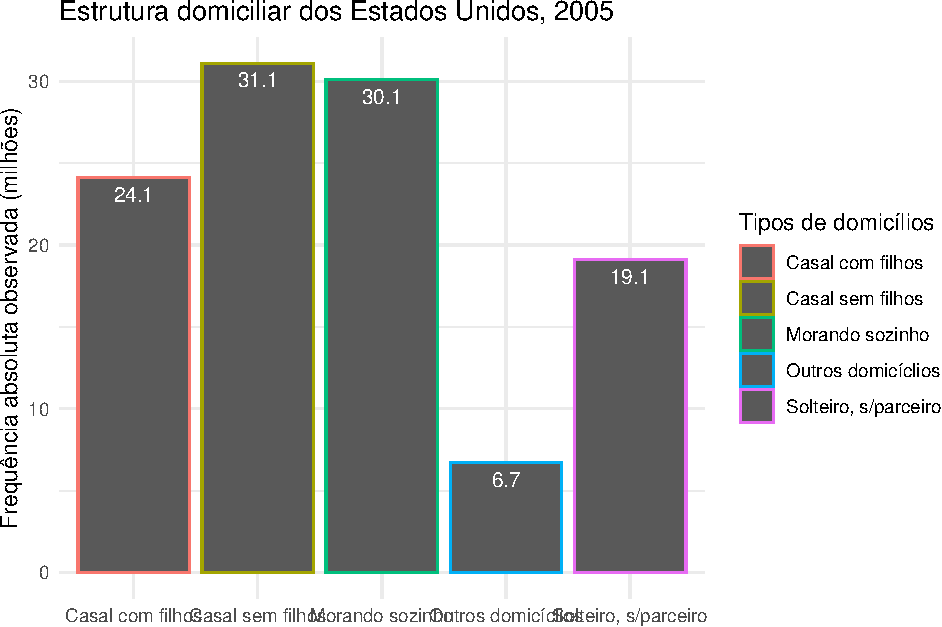
\includegraphics{apostila_files/figure-latex/unnamed-chunk-48-1.pdf}
\caption{\label{fig:unnamed-chunk-48}Gráfico de barras dos dados brutos: uma barra para cada observação e sua altura expressando o número de observações com esse valor}
\end{figure}

\hfill\break

\hypertarget{histograma}{%
\subsection{Histograma}\label{histograma}}

\hfill\break

Para dados quantitativos, o agrupamento dos valores brutos observados em classes (cada uma com um valor mínimo e máximo fixado) permite a geração de um \emph{Histograma}, um tipo diferente de \emph{Gráfico de barras} onde cada coluna está unida às colunas imediatamente adjacentes (indicando a continuidade de valores das medidas) e sua altura expressa a quantidade de observações contidas nessa classe.

\hfill\break

Para as classes estabelecias na seção anterior o histograma das alturas dos estudantes terá esse aspecto:

\hfill\break

\begin{Shaded}
\begin{Highlighting}[]
\NormalTok{h1}\OtherTok{=}\FunctionTok{hist}\NormalTok{(alturas, }\AttributeTok{breaks=}\FunctionTok{seq}\NormalTok{(}\FloatTok{1.41}\NormalTok{ , }\FloatTok{2.01}\NormalTok{ , }\FloatTok{0.1}\NormalTok{), }\AttributeTok{main=} \StringTok{"Histograma das alturas dos estudantes"}\NormalTok{, }\AttributeTok{col=}\StringTok{"blue"}\NormalTok{, }
\AttributeTok{xlab=}\StringTok{"Classes de alturas (m)"}\NormalTok{, }\AttributeTok{ylab=}\StringTok{"Frequência absoluta observada (un)"}\NormalTok{ , }\AttributeTok{cex=}\FloatTok{0.7}\NormalTok{, }\AttributeTok{ylim=}\FunctionTok{c}\NormalTok{(}\DecValTok{0}\NormalTok{,}\DecValTok{30}\NormalTok{))}
\FunctionTok{text}\NormalTok{(h1}\SpecialCharTok{$}\NormalTok{mids,h1}\SpecialCharTok{$}\NormalTok{counts,}\AttributeTok{labels=}\NormalTok{h1}\SpecialCharTok{$}\NormalTok{counts, }\AttributeTok{adj=}\FunctionTok{c}\NormalTok{(}\FloatTok{0.5}\NormalTok{, }\SpecialCharTok{{-}}\FloatTok{0.5}\NormalTok{))}
\FunctionTok{abline}\NormalTok{(}\AttributeTok{v=}\FunctionTok{mean}\NormalTok{(alturas), }\AttributeTok{col=}\StringTok{"red"}\NormalTok{) }
\FunctionTok{text}\NormalTok{(}\FunctionTok{mean}\NormalTok{(alturas)}\SpecialCharTok{{-}}\FloatTok{0.01}\NormalTok{, }\DecValTok{28}\NormalTok{, }\StringTok{"Média=1,69 m"}\NormalTok{, }\AttributeTok{col =} \StringTok{"red"}\NormalTok{, }\AttributeTok{srt=}\DecValTok{90}\NormalTok{)}
\FunctionTok{abline}\NormalTok{(}\AttributeTok{v=}\FunctionTok{median}\NormalTok{(alturas), }\AttributeTok{col=}\StringTok{"darkgreen"}\NormalTok{) }
\FunctionTok{text}\NormalTok{(}\FunctionTok{median}\NormalTok{(alturas)}\SpecialCharTok{{-}}\FloatTok{0.01}\NormalTok{, }\FloatTok{27.2}\NormalTok{, }\StringTok{"Mediana=1,675 m"}\NormalTok{, }\AttributeTok{col =} \StringTok{"darkgreen"}\NormalTok{, }\AttributeTok{srt=}\DecValTok{90}\NormalTok{)}
\FunctionTok{abline}\NormalTok{(}\AttributeTok{v=}\FunctionTok{Modes}\NormalTok{(alturas), }\AttributeTok{col=}\StringTok{"darkgrey"}\NormalTok{) }
\FunctionTok{text}\NormalTok{(}\FunctionTok{Modes}\NormalTok{(alturas)}\SpecialCharTok{+}\FunctionTok{c}\NormalTok{(}\SpecialCharTok{{-}}\FloatTok{0.01}\NormalTok{, }\SpecialCharTok{{-}}\FloatTok{0.01}\NormalTok{), }\DecValTok{27}\NormalTok{, }\FunctionTok{c}\NormalTok{(}\StringTok{"Moda=1,66"}\NormalTok{,}\StringTok{"Moda=1,73"}\NormalTok{), }\AttributeTok{col =} \StringTok{"darkgray"}\NormalTok{, }\AttributeTok{srt=}\DecValTok{90}\NormalTok{)}
\end{Highlighting}
\end{Shaded}

\begin{figure}

{\centering 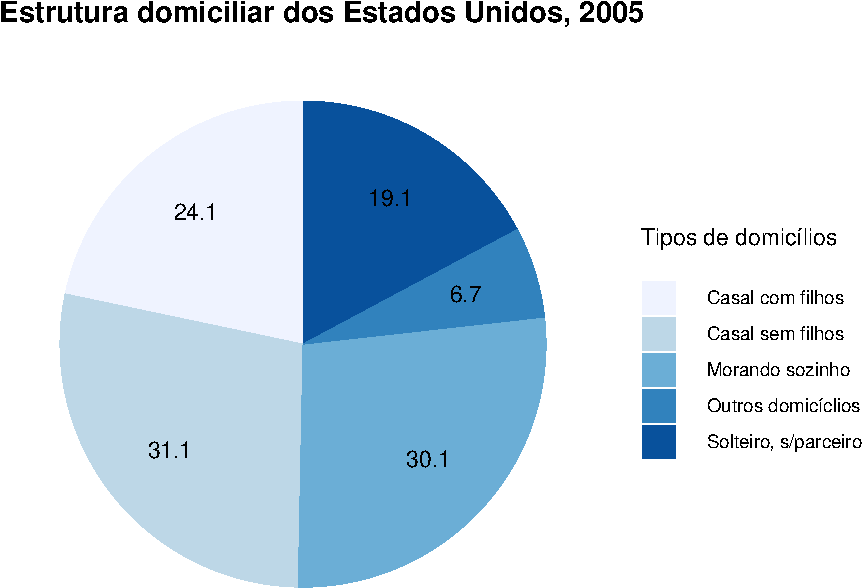
\includegraphics[width=0.8\linewidth]{apostila_files/figure-latex/unnamed-chunk-49-1} 

}

\caption{Histograma das alturas dos estudantes com as posições da média, moda e mediana}\label{fig:unnamed-chunk-49}
\end{figure}

\hfill\break

Um \emph{histograma} é a representação gráfica de uma \emph{tabela de distribuição de frequências} em colunas (retângulos).

\hfill\break

A base de cada retângulo representa o intervalo de cada classe e a altura, a quantidade ou a \emph{frequência absoluta} com que aquele valor da classe ocorre no conjunto de dados.

\hfill\break

O termo \emph{histograma} foi cunhado por Karl Pearson (c.~1891) e vem da composição em grego de \emph{istos} (mastro) com \emph{gramma} (escrita), convertida em inglês para \emph{historical diagram: histogram}.

\hfill\break

Como elemento gráfico, seu uso é anterior à sua denominação (maiores detalhes em:
\href{https://www.ine.es/ss/Satellite?blobcol=urldata\&blobheader=application\%2Fpdf\&blobheadername1=Content-Disposition\&blobheadervalue1=attachment\%3B+filename\%3Dart_192_2.pdf\&blobkey=urldata\&blobtable=MungoBlobs\&blobwhere=229\%2F670\%2Fart_192_2.pdf\&ssbinary=true}{(link)} ).

\hfill\break

Num histograma de densidade, a altura de cada retângulo representa a densidade da ocorrência da \emph{frequência relativa}.

\hfill\break

\begin{Shaded}
\begin{Highlighting}[]
\NormalTok{h2}\OtherTok{=}\FunctionTok{hist}\NormalTok{(alturas,}\AttributeTok{breaks=}\FunctionTok{seq}\NormalTok{(}\FloatTok{1.41}\NormalTok{ , }\FloatTok{2.01}\NormalTok{ , }\FloatTok{0.10}\NormalTok{), }\AttributeTok{main=} \StringTok{"Histograma das alturas dos estudantes"}\NormalTok{, }\AttributeTok{col=}\StringTok{"blue"}\NormalTok{, }
\AttributeTok{xlab=}\StringTok{"Classes de alturas (m)"}\NormalTok{, }\AttributeTok{ylab=}\StringTok{"Densidade da freq. relativa"}\NormalTok{, }\AttributeTok{prob=}\StringTok{"TRUE"}\NormalTok{, }\AttributeTok{ylim=}\FunctionTok{c}\NormalTok{(}\DecValTok{0}\NormalTok{,}\DecValTok{5}\NormalTok{))}
\FunctionTok{text}\NormalTok{(h2}\SpecialCharTok{$}\NormalTok{mids,h2}\SpecialCharTok{$}\NormalTok{density,}\AttributeTok{labels=}\FunctionTok{round}\NormalTok{(h2}\SpecialCharTok{$}\NormalTok{density, }\DecValTok{5}\NormalTok{), }\AttributeTok{adj=}\FunctionTok{c}\NormalTok{(}\FloatTok{0.5}\NormalTok{, }\SpecialCharTok{{-}}\FloatTok{0.5}\NormalTok{), }\AttributeTok{cex=}\FloatTok{0.7}\NormalTok{)}
\FunctionTok{lines}\NormalTok{(}\FunctionTok{density}\NormalTok{(alturas), }\AttributeTok{col=}\StringTok{"red"}\NormalTok{)             }
\FunctionTok{lines}\NormalTok{(}\FunctionTok{density}\NormalTok{(alturas, }\AttributeTok{adjust=}\DecValTok{2}\NormalTok{), }\AttributeTok{col=}\StringTok{"orange"}\NormalTok{)  }
\end{Highlighting}
\end{Shaded}

\begin{figure}
\centering
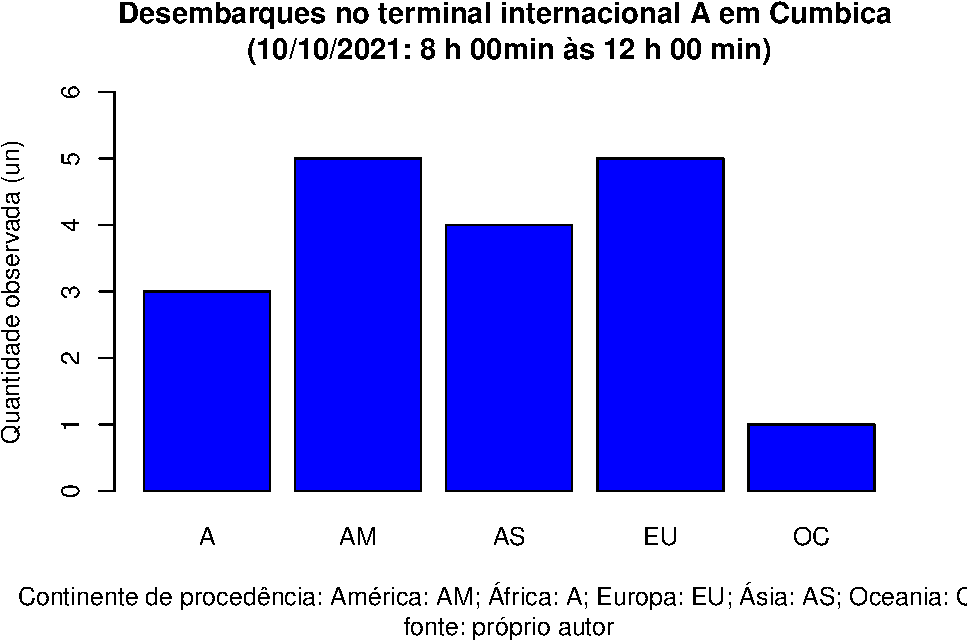
\includegraphics{apostila_files/figure-latex/unnamed-chunk-50-1.pdf}
\caption{\label{fig:unnamed-chunk-50}A linha vermelha é uma aproximação da Função de Densidade da frequência relativa de observação (a linha preta é a curva da função densidade de uma distribuição Normal com média e variâncias dadas pelos dados}
\end{figure}

\hfill\break

Como a área de cada retângulo é igual à proporção (\(fr_{i}\)) da classe (\(i\)) a soma de todas essas áreas será igual a 1:

\hfill\break

\begin{Shaded}
\begin{Highlighting}[]
\NormalTok{(}\FloatTok{0.10}\SpecialCharTok{*}\FloatTok{0.5}\NormalTok{)}\SpecialCharTok{+}\NormalTok{(}\FloatTok{0.10}\SpecialCharTok{*}\FloatTok{1.333}\NormalTok{)}\SpecialCharTok{+}\NormalTok{(}\FloatTok{0.10}\SpecialCharTok{*}\FloatTok{3.833}\NormalTok{)}\SpecialCharTok{+}\NormalTok{(}\FloatTok{0.10}\SpecialCharTok{*}\FloatTok{2.833}\NormalTok{)}\SpecialCharTok{+}\NormalTok{(}\FloatTok{0.10}\SpecialCharTok{*}\DecValTok{1}\NormalTok{)}\SpecialCharTok{+}\NormalTok{(}\FloatTok{0.10}\SpecialCharTok{*}\FloatTok{0.50}\NormalTok{)}
\end{Highlighting}
\end{Shaded}

\begin{verbatim}
## [1] 0.9999
\end{verbatim}

\hfill\break

Uma aproximação para a \textbf{área sob a curva da Função de Densidade} pode ser soma das áreas de um dos retângulo com:

\hfill\break

\begin{itemize}
\tightlist
\item
  Base = \(\Delta_{i}\); e,\textbackslash{}
\item
  Altura =\(\frac{fr_{i}}{\Delta_{i}}\).
\end{itemize}

\hfill\break

A \textbf{área da curva da Função de Densidade delimitada por dois valores quaisquer} é uma analogia para a probabilidade de que um determinado valor de altura de um estudante (amostrado aleatoriamente dentre todos os 60 estudantes) esteja contida nesse intervalo.

\hfill\break

\textbf{Equivale dizer que}, amostrando-se aleatoriamente um estudante dentre todos os 60 alunos, a probabilidade de que a altura desse estudante estaje contida entre os valores mínimo e máximo da amostra é, \textbf{naturalmente}, igual a 1 (100\%)

\hypertarget{setores}{%
\subsection{Setores}\label{setores}}

\hfill\break

Em um \emph{Gráfico de setores} a representação das quantidades está associada a uma fração do comprimento de um círculo. Para sua confecção considera-se a proporção da quantidade observada específica da quantidade total de dados, expressa na forma de fração do ângulo de um setor circular em relação ao ângulo interno total de um círculo (360\textsuperscript{o}).

\hfill\break
\hfill\break

\begin{Shaded}
\begin{Highlighting}[]
\FunctionTok{library}\NormalTok{(scales)}
\FunctionTok{library}\NormalTok{(ggplot2)}

\NormalTok{alturas\_classes}\OtherTok{=}\FunctionTok{data.frame}\NormalTok{(}
  \AttributeTok{group =} \FunctionTok{c}\NormalTok{(}\StringTok{"1,41{-}1,51"}\NormalTok{,}
            \StringTok{"1,51{-}1,61"}\NormalTok{,}
            \StringTok{"1,61{-}1,71"}\NormalTok{,}
            \StringTok{"1,71{-}1,81"}\NormalTok{,}
            \StringTok{"1,81{-}1,91"}\NormalTok{,}
            \StringTok{"1,91{-}2,01"}\NormalTok{),}
  \AttributeTok{value =} \FunctionTok{c}\NormalTok{(}\DecValTok{3}\NormalTok{,}\DecValTok{8}\NormalTok{,}\DecValTok{23}\NormalTok{,}\DecValTok{17}\NormalTok{,}\DecValTok{6}\NormalTok{,}\DecValTok{3}\NormalTok{))}

\NormalTok{blank\_theme}\OtherTok{=}\FunctionTok{theme\_minimal}\NormalTok{()}\SpecialCharTok{+}
  \FunctionTok{theme}\NormalTok{(}
    \AttributeTok{axis.title.x =} \FunctionTok{element\_blank}\NormalTok{(),}
    \AttributeTok{axis.title.y =} \FunctionTok{element\_blank}\NormalTok{(),}
    \AttributeTok{panel.border =} \FunctionTok{element\_blank}\NormalTok{(),}
    \AttributeTok{panel.grid=}\FunctionTok{element\_blank}\NormalTok{(),}
    \AttributeTok{axis.ticks =} \FunctionTok{element\_blank}\NormalTok{(),}
    \AttributeTok{plot.title=}\FunctionTok{element\_text}\NormalTok{(}\AttributeTok{size=}\DecValTok{14}\NormalTok{, }\AttributeTok{face=}\StringTok{"bold"}\NormalTok{)}
\NormalTok{  )}

\FunctionTok{ggplot}\NormalTok{(alturas\_classes, }\FunctionTok{aes}\NormalTok{(}\AttributeTok{x=}\StringTok{""}\NormalTok{, }\AttributeTok{y=}\NormalTok{value, }\AttributeTok{fill=}\NormalTok{group)) }\SpecialCharTok{+}
\NormalTok{  blank\_theme }\SpecialCharTok{+}
  \FunctionTok{scale\_fill\_brewer}\NormalTok{(}\StringTok{"Blues"}\NormalTok{)}\SpecialCharTok{+}
  \FunctionTok{ggtitle}\NormalTok{(}\StringTok{"Alturas dos estudantes"}\NormalTok{) }\SpecialCharTok{+}
  \FunctionTok{theme}\NormalTok{(}\AttributeTok{axis.text.x=}\FunctionTok{element\_blank}\NormalTok{()) }\SpecialCharTok{+}
  \FunctionTok{geom\_bar}\NormalTok{(}\AttributeTok{width =} \DecValTok{1}\NormalTok{, }\AttributeTok{stat =} \StringTok{"identity"}\NormalTok{) }\SpecialCharTok{+}
  \FunctionTok{coord\_polar}\NormalTok{(}\StringTok{"y"}\NormalTok{, }\AttributeTok{start=}\DecValTok{0}\NormalTok{) }\SpecialCharTok{+}
  \FunctionTok{geom\_text}\NormalTok{(}\FunctionTok{aes}\NormalTok{(}\AttributeTok{y =}\NormalTok{ value}\SpecialCharTok{/}\DecValTok{2} \SpecialCharTok{+} \FunctionTok{c}\NormalTok{(}\DecValTok{0}\NormalTok{, }\FunctionTok{cumsum}\NormalTok{(value)[}\SpecialCharTok{{-}}\FunctionTok{length}\NormalTok{(value)]),}
                \AttributeTok{label =} \FunctionTok{percent}\NormalTok{(value}\SpecialCharTok{/}\DecValTok{60}\NormalTok{ )), }\AttributeTok{size=}\DecValTok{5}\NormalTok{)}\SpecialCharTok{+}
  \FunctionTok{guides}\NormalTok{(}\AttributeTok{fill =} \FunctionTok{guide\_legend}\NormalTok{(}\StringTok{"Classes de valores (m)"}\NormalTok{,}
                             \AttributeTok{label.position =} \StringTok{"right"}\NormalTok{,}
                             \AttributeTok{title.position =} \StringTok{"top"}\NormalTok{, }\AttributeTok{title.vjust =} \DecValTok{1}\NormalTok{)) }
\end{Highlighting}
\end{Shaded}

\begin{figure}
\centering
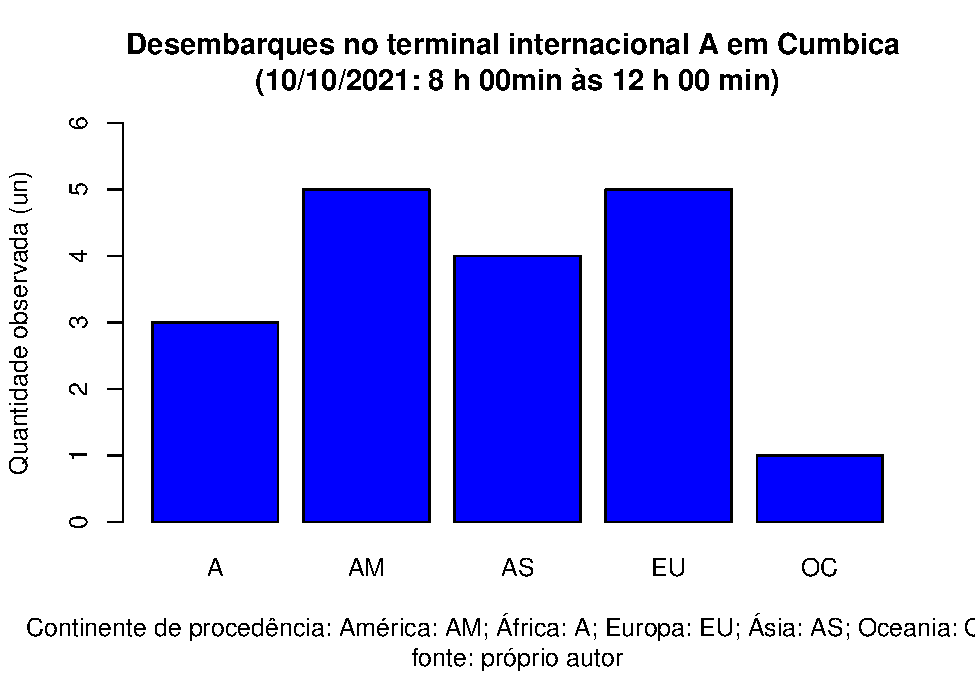
\includegraphics{apostila_files/figure-latex/unnamed-chunk-52-1.pdf}
\caption{\label{fig:unnamed-chunk-52}Gráfico de setores das alturas dos estudantes}
\end{figure}

\hfill\break

\hypertarget{box-plot}{%
\subsection{Box-plot}\label{box-plot}}

\hfill\break

O gráfico \textbf{Box-plot} ( \emph{box and whisker plot} ): esse gráfico apresenta de modo conjunto, informações sobre a posição, dispersão, assimetria e dados discrepantes do conjunto analisado:

\hfill\break

\begin{itemize}
\tightlist
\item
  a mediana (\(Q_{2}\));
\item
  os valores mínimo: \(x_{1}\) e máximo: \(x_{n}\) (dados ordenados);
\item
  o 1\(^{o}\) e 3\(^{o}\) quartis;
\item
  a dispersão (intervalo interquartílico: \(d_{q}=(Q_{3} - Q_{1})\));
\item
  os limites superior: \(LS=Q_{3} + 1,50.d_{q}\), e inferior: \(LI=Q_{1} - 1,50.d_{q}\) ( \emph{bigodes});
\item
  os valores mínimo e máximo observados (caso não existam valores superiores aos limites \emph{LI} e \emph{LS}); ou
\item
  as observações mais extremas, situadas fora dos limites \emph{LI} e \emph{LS} (que \textbf{podem ou não} ser \emph{outliers} , dados atípicos).
\end{itemize}

\hfill\break

\begin{Shaded}
\begin{Highlighting}[]
\NormalTok{min}\OtherTok{=}\FunctionTok{min}\NormalTok{(alturas)}
\NormalTok{q1}\OtherTok{=}\FloatTok{1.635}
\NormalTok{q2}\OtherTok{=}\FloatTok{1.675}
\NormalTok{med}\OtherTok{=}\FunctionTok{mean}\NormalTok{(alturas)}
\NormalTok{q3}\OtherTok{=}\FloatTok{1.755}
\NormalTok{max}\OtherTok{=}\FunctionTok{max}\NormalTok{(alturas)}
\NormalTok{iq}\OtherTok{=}\NormalTok{q3}\SpecialCharTok{{-}}\NormalTok{q1}
\NormalTok{ls}\OtherTok{=}\NormalTok{q3}\FloatTok{+1.5}\SpecialCharTok{*}\NormalTok{iq}
\NormalTok{li}\OtherTok{=}\NormalTok{q1}\FloatTok{{-}1.5}\SpecialCharTok{*}\NormalTok{iq}
\FunctionTok{head}\NormalTok{(}\FunctionTok{sort}\NormalTok{(alturas,}\ConstantTok{TRUE}\NormalTok{)) }\CommentTok{\#2.00 1.95 \textgreater{}\textgreater{}1.93\textless{}\textless{} 1.86 1.85 1.84}
\end{Highlighting}
\end{Shaded}

\begin{verbatim}
## [1] 2.00 1.95 1.93 1.86 1.85 1.84
\end{verbatim}

\begin{Shaded}
\begin{Highlighting}[]
\FunctionTok{tail}\NormalTok{(}\FunctionTok{sort}\NormalTok{(alturas,}\ConstantTok{TRUE}\NormalTok{)) }\CommentTok{\# 1.56 1.55 1.54 1.47 1.44 \textgreater{}\textgreater{}1.41\textless{}\textless{}}
\end{Highlighting}
\end{Shaded}

\begin{verbatim}
## [1] 1.56 1.55 1.54 1.47 1.44 1.41
\end{verbatim}

\begin{Shaded}
\begin{Highlighting}[]
\FunctionTok{boxplot}\NormalTok{(alturas, }
        \AttributeTok{main=}\StringTok{"Boxplot do conjunto de dados de alturas }\SpecialCharTok{\textbackslash{}n}\StringTok{(média=1,69 ; mediana=1,675 ; min=1,41 ; máx=2,00 ; Q1=1,635 ; Q3=1,755 ; iq=0,12 , LS=1,935  ; LI=1,455 )"}\NormalTok{,}
        \AttributeTok{ylim=}\FunctionTok{c}\NormalTok{(}\FloatTok{1.3}\NormalTok{, }\FloatTok{2.1}\NormalTok{))}
\FunctionTok{lines}\NormalTok{( }\AttributeTok{y=}\FunctionTok{c}\NormalTok{(min, min), }\AttributeTok{x=}\FunctionTok{c}\NormalTok{(}\FloatTok{0.6}\NormalTok{,}\DecValTok{1}\NormalTok{), }\AttributeTok{col=}\StringTok{"red"}\NormalTok{) }
\FunctionTok{text}\NormalTok{(}\AttributeTok{x=}\FloatTok{0.60}\NormalTok{, }\AttributeTok{y=}\NormalTok{min}\FloatTok{{-}0.05}\NormalTok{, }\StringTok{"Valor mínimo observado"}\NormalTok{, }\AttributeTok{col =} \StringTok{"red"}\NormalTok{, }\AttributeTok{srt=}\DecValTok{0}\NormalTok{)}
\FunctionTok{lines}\NormalTok{( }\AttributeTok{y=}\FunctionTok{c}\NormalTok{(max,max), }\AttributeTok{x=}\FunctionTok{c}\NormalTok{(}\FloatTok{0.6}\NormalTok{,}\DecValTok{1}\NormalTok{), }\AttributeTok{col=}\StringTok{"red"}\NormalTok{) }
\FunctionTok{text}\NormalTok{(}\AttributeTok{x=}\FloatTok{0.60}\NormalTok{, }\AttributeTok{y=}\NormalTok{max}\FloatTok{+0.05}\NormalTok{, }\StringTok{"Valor máximo observado"}\NormalTok{, }\AttributeTok{col =} \StringTok{"red"}\NormalTok{, }\AttributeTok{srt=}\DecValTok{0}\NormalTok{)}
\FunctionTok{lines}\NormalTok{(}\AttributeTok{y=}\FunctionTok{c}\NormalTok{(med, med),  }\AttributeTok{x=}\FunctionTok{c}\NormalTok{(}\DecValTok{1}\NormalTok{,}\FloatTok{1.4}\NormalTok{), }\AttributeTok{col=}\StringTok{"red"}\NormalTok{) }
\FunctionTok{text}\NormalTok{(}\AttributeTok{x=}\FloatTok{1.4}\NormalTok{ , }\AttributeTok{y=}\NormalTok{ med}\FloatTok{+0.02}\NormalTok{ , }\StringTok{"Média"}\NormalTok{, }\AttributeTok{col =} \StringTok{"red"}\NormalTok{, }\AttributeTok{srt=}\DecValTok{0}\NormalTok{)}
\FunctionTok{lines}\NormalTok{(}\AttributeTok{y=}\FunctionTok{c}\NormalTok{(q1, q1), }\AttributeTok{x=}\FunctionTok{c}\NormalTok{(}\DecValTok{1}\NormalTok{, }\FloatTok{1.4}\NormalTok{), }\AttributeTok{col=}\StringTok{"red"}\NormalTok{) }
\FunctionTok{text}\NormalTok{(}\AttributeTok{x=}\FloatTok{1.4}\NormalTok{, }\AttributeTok{y=}\NormalTok{q1 }\SpecialCharTok{{-}}\FloatTok{0.05}\NormalTok{, }\StringTok{"Primeiro quartil (Q1)"}\NormalTok{, }\AttributeTok{col =} \StringTok{"red"}\NormalTok{, }\AttributeTok{srt=}\DecValTok{0}\NormalTok{)}
\FunctionTok{lines}\NormalTok{(}\AttributeTok{y=}\FunctionTok{c}\NormalTok{(q2, q2),  }\AttributeTok{x=}\FunctionTok{c}\NormalTok{(}\FloatTok{0.6}\NormalTok{,}\DecValTok{1}\NormalTok{), }\AttributeTok{col=}\StringTok{"red"}\NormalTok{) }
\FunctionTok{text}\NormalTok{(}\AttributeTok{x=}\FloatTok{0.60}\NormalTok{ , }\AttributeTok{y=}\NormalTok{ q2 }\SpecialCharTok{{-}} \FloatTok{0.05}\NormalTok{, }\StringTok{"Mediana (Q2)"}\NormalTok{, }\AttributeTok{col =} \StringTok{"red"}\NormalTok{, }\AttributeTok{srt=}\DecValTok{0}\NormalTok{)}
\FunctionTok{lines}\NormalTok{(}\AttributeTok{y=}\FunctionTok{c}\NormalTok{(q3, q3), }\AttributeTok{x=}\FunctionTok{c}\NormalTok{(}\DecValTok{1}\NormalTok{, }\FloatTok{1.4}\NormalTok{), }\AttributeTok{col=}\StringTok{"red"}\NormalTok{) }
\FunctionTok{text}\NormalTok{(}\AttributeTok{x=} \FloatTok{1.4}\NormalTok{ , }\AttributeTok{y=}\NormalTok{q3 }\SpecialCharTok{+} \FloatTok{0.05}\NormalTok{, }\StringTok{"Terceiro quartil (Q3)"}\NormalTok{, }\AttributeTok{col =} \StringTok{"red"}\NormalTok{, }\AttributeTok{srt=}\DecValTok{0}\NormalTok{)}
\FunctionTok{lines}\NormalTok{(}\AttributeTok{y=}\FunctionTok{c}\NormalTok{(li,li) , }\AttributeTok{x=}\FunctionTok{c}\NormalTok{(}\FloatTok{1.01}\NormalTok{,}\FloatTok{1.4}\NormalTok{) , }\AttributeTok{col=}\StringTok{"blue"}\NormalTok{, }\AttributeTok{lty=}\DecValTok{2}\NormalTok{) }
\FunctionTok{text}\NormalTok{(}\AttributeTok{x=}\FloatTok{1.2}\NormalTok{, }\AttributeTok{y=}\NormalTok{q1}\FloatTok{{-}1.5}\SpecialCharTok{*}\NormalTok{iq}\FloatTok{{-}0.05}\NormalTok{ , }\StringTok{"Limite inferior teórico (LI=1,455) "}\NormalTok{, }\AttributeTok{col =} \StringTok{"blue"}\NormalTok{, }\AttributeTok{srt=}\DecValTok{0}\NormalTok{)}
\FunctionTok{lines}\NormalTok{(}\AttributeTok{y=}\FunctionTok{c}\NormalTok{(ls,ls) , }\AttributeTok{x=}\FunctionTok{c}\NormalTok{(}\FloatTok{1.01}\NormalTok{,}\FloatTok{1.4}\NormalTok{) , }\AttributeTok{col=}\StringTok{"blue"}\NormalTok{, }\AttributeTok{lty=}\DecValTok{2}\NormalTok{) }
\FunctionTok{text}\NormalTok{(}\AttributeTok{x=}\FloatTok{1.2}\NormalTok{, }\AttributeTok{y=}\NormalTok{q3}\FloatTok{+1.5}\SpecialCharTok{*}\NormalTok{iq }\SpecialCharTok{+}\FloatTok{0.05}\NormalTok{ , }\StringTok{"Limite superior teórico (LS=1,935)"}\NormalTok{, }\AttributeTok{col =} \StringTok{"blue"}\NormalTok{, }\AttributeTok{srt=}\DecValTok{0}\NormalTok{)}
\FunctionTok{lines}\NormalTok{(}\AttributeTok{y=}\FunctionTok{c}\NormalTok{(}\FloatTok{1.47}\NormalTok{,}\FloatTok{1.47}\NormalTok{) , }\AttributeTok{x=}\FunctionTok{c}\NormalTok{(}\FloatTok{0.85}\NormalTok{,}\FloatTok{0.95}\NormalTok{) , }\AttributeTok{col=}\StringTok{"green"}\NormalTok{, }\AttributeTok{lty=}\DecValTok{2}\NormalTok{) }
\FunctionTok{text}\NormalTok{(}\AttributeTok{x=}\FloatTok{0.7}\NormalTok{, }\AttributeTok{y=}\FloatTok{1.47}\NormalTok{ , }\StringTok{"Última observação dentro do LI (x=1,47) "}\NormalTok{, }\AttributeTok{col =} \StringTok{"green"}\NormalTok{, }\AttributeTok{srt=}\DecValTok{0}\NormalTok{)}
\FunctionTok{lines}\NormalTok{(}\AttributeTok{y=}\FunctionTok{c}\NormalTok{(}\FloatTok{1.93}\NormalTok{,}\FloatTok{1.93}\NormalTok{) , }\AttributeTok{x=}\FunctionTok{c}\NormalTok{(}\FloatTok{0.85}\NormalTok{,}\FloatTok{0.95}\NormalTok{) , }\AttributeTok{col=}\StringTok{"green"}\NormalTok{, }\AttributeTok{lty=}\DecValTok{2}\NormalTok{) }
\FunctionTok{text}\NormalTok{(}\AttributeTok{x=}\FloatTok{0.7}\NormalTok{, }\AttributeTok{y=}\FloatTok{1.93}\NormalTok{ , }\StringTok{"Última observação dentro do LS (x=1,86) "}\NormalTok{, }\AttributeTok{col =} \StringTok{"green"}\NormalTok{, }\AttributeTok{srt=}\DecValTok{0}\NormalTok{)}
\end{Highlighting}
\end{Shaded}

\begin{figure}

{\centering 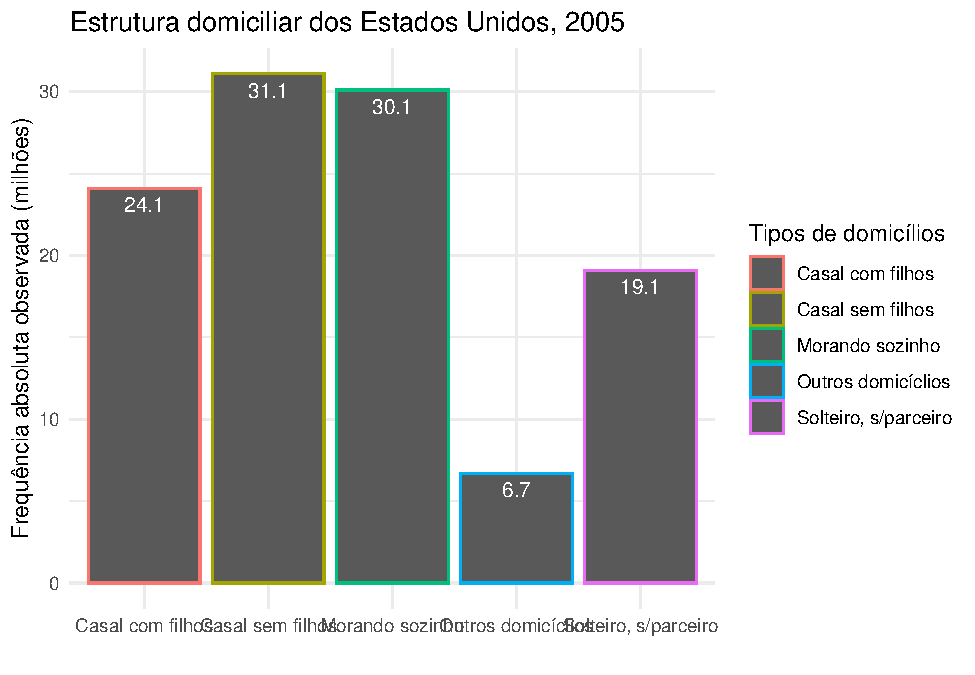
\includegraphics{apostila_files/figure-latex/unnamed-chunk-53-1} 

}

\caption{Box-plot de um rol de valores com Distribuição Normal (média 20 e variãncia 5}\label{fig:unnamed-chunk-53}
\end{figure}

\hypertarget{introduuxe7uxe3o-ao-cuxe1lculo-de-probabilidades}{%
\chapter{Introdução ao cálculo de probabilidades}\label{introduuxe7uxe3o-ao-cuxe1lculo-de-probabilidades}}

Seria bom começar um curso sobre teoria das probabilidades, dando uma definição de probabilidade concisa, simples e intuitiva, mas rigorosa. Infelizmente, isto não será possível.

\hfill\break

Se por um lado, uma definição rigorosa de probabilidade requer um aparato matemático sofisticado e é bem pouco intuitiva; por outro lado, definições simples são frequentemente enganosas ou, na melhor das hipóteses, tautológicas .

\hfill\break

Por exemplo, poderíamos dizer que probabilidade:

\hfill\break

\begin{quote}
é um \emph{número} que quantifica, uma \emph{medida da informação} disponível sobre a possibilidade de ocorrência de um determinado \emph{evento} quando ainda não se sabe se ele ocorrerá ou não.
\end{quote}

\hfill\break

Essa definição é circular (\emph{definiendum=definien} porque usa o conceito de probabilidade, que é um sinônimo de possibilidade, chance, esperança, viabilidade, exequibilidade, expectativa, \dots).

\hfill\break

Todavia ela nos introduz \textbf{dois conceitos} que iremos usar como ponto de partida:

\hfill\break

\begin{enumerate}
\def\labelenumi{\arabic{enumi}.}
\tightlist
\item
  probabilidade refere-se a \emph{experimentos aleatórios} e seus \emph{eventos}; e,
\item
  probabilidade é um \emph{número}.
\end{enumerate}

\hfill\break

O \emph{conceito clássico} de probabilidade será a seguir apresentado e, ao final será abordado o conceito de probabilidade como uma função matemática alicerçada em alguns postulados ( \emph{conceito axiomático} ).

\hypertarget{introduuxe7uxe3o-conceitual-essencial-1}{%
\section{Introdução conceitual essencial}\label{introduuxe7uxe3o-conceitual-essencial-1}}

\hypertarget{experimentos-determinuxedsticos-e-experimentos-probabiluxedsticos-aleatuxf3rios}{%
\subsection{Experimentos determinísticos e experimentos probabilísticos (aleatórios)}\label{experimentos-determinuxedsticos-e-experimentos-probabiluxedsticos-aleatuxf3rios}}

Aleatório provem do latim: \emph{aleatorium}: fato cujo desfecho depende de um acontecimento futuro e incerto, resultado da sorte ou acaso, acidental.

\hfill\break

Ao contrário de um \textbf{experimento determinístico}, cujo resultado pode ser previamente determinado (como a reação de dois átomos de \emph{H} com um átomo de \emph{O} ou a distância percorrida - no vácuo sob velocidade constante e sem atrito - por um objeto \(S = V \times t\)), o conceito de experimento aleatório é o que estabelece que seu resultado \textbf{não pode ser previsto com certeza}.\\

Os resultados observados \textbf{apresentam variações} mesmo quando esses experimentos são repetidos indefinidamente e sob as mesmas condições; todavia, é possível estabelecer um conjunto cujos elementos compõem todos os possíveis resultados.

\hfill\break

\hypertarget{espauxe7o-amostral-e-seus-elementos}{%
\subsection{Espaço amostral e seus elementos}\label{espauxe7o-amostral-e-seus-elementos}}

A primeira coisa que fazemos quando começamos a pensar sobre a probabilidade de ocorrência de um certo resultado em um \textbf{experimento aleatório} é listar \textbf{todos os resultados com possibilidade de ocorrência}.

\hfill\break

Esses resultados são os elementos de um conjunto a que denominamos de \emph{espaço amostral} e, usualmente o representamos pela letra grega maiúscula \(\Omega\).

\hfill\break

Para que \(\Omega\) seja considerado o \emph{espaço amostral} desse experimento aleatório ele precisa apresentar duas propriedades:

\hfill\break

1- \textbf{apenas um} de seus elementos pode ocorrer ao se realizar o \emph{experimento aleatório} (\textbf{resultado}); e,
2- \textbf{ao menos um} dos possíveis resultados deverá ocorrer.

\hfill\break

Tais propriedades são equivalentes a se dizer que os elementos do espaço amostral, os \textbf{resultados}listados como possibilidades de se verificar ao se realizar um \textbf{experimento aleatório} são \textbf{mutuamente exclusivos e exaustivos}.

\hfill\break

Exemplos clássicos de experimentos aleatórios são o \emph{lançamento de moedas}, \emph{dados} ou extração de \emph{cartas de um baralho}.

\hfill\break

Os possíveis resultados como a face de uma moeda ou o número que um dado irá expor ao ser lançado, \textbf{embora não possam ser antecipados com certeza}, encontram-se limitados a um conjunto de todas as uas possibilidades, seu \textbf{espaço amostral}.

\hfill\break

Para o lançamento de um dado:

\hfill\break

\[
\Omega = \{ 1,2,3,4,5,6\}
\]

\hfill\break

e para o lançamento de uma moeda

\hfill\break

\[
\Omega=\{\text{cara}, \text{coroa}\}
\].

\hfill\break

Um espaço amostral consiste então da enumeração (finita ou infinita) de todos os resultados possíveis de serem gerados em um experimento aleatório, generalizado como sendo o conjunto

\hfill\break

\[
\Omega = \{\omega_{1}, \omega_{2}, \omega_{3}, ..., \omega_{n}, \dots \}
\]

\hfill\break

\textbf{Cada um} dos possíveis resultados de um experimento aleatório com espaço amostral \(\Omega\) é chamado de um \textbf{elemento} desse espaço amostral e é denotado pela letra grega: \(\omega_{n}\).

\hfill\break

\hypertarget{evento-de-interesse-sucesso}{%
\subsection{Evento de interesse (sucesso)}\label{evento-de-interesse-sucesso}}

\hypertarget{evento}{%
\subsection{Evento}\label{evento}}

Denomina-se como \textbf{evento} um \textbf{subconjunto} finito do \textbf{espaço amostral} composto por um ou mais de seus elementos, e que \textbf{satisfazem (atendem)} ao enunciado definido no experimento aleatório desejado.

\hfill\break

A expressão \textbf{evento de interesse} (ou sucesso) define, para o cálculo de probabilidades, a ocorrência de um resultado previamente definido no experimento aleatório.

\hfill\break

Admita um \textbf{experimento aleatório} que consiste em se lançar um dado uma vez. Um \textbf{evento de interesse} pode ser definido como sendo obter um número par. A partir dessas condições, pode-se calcular-se a probabilidade de se obter \textbf{sucesso} no experimento aleatório; isto é, obter-se um número par ao se lançar um dado uma vez.

\hfill\break

Admita um outro experimento aleatório que agora consiste em se lançar uma moeda duas vezes.

\hfill\break

O \textbf{espaço amostral} desse experimento aleatório (\textbf{todos os possíveis resultados}) será um conjunto composto por quatro elementos:

\hfill\break

\[
\Omega = \{\omega_{1}, \omega_{2}, \omega_{3}, \omega_{4}\}
\]

\hfill\break

onde:

\hfill\break

\begin{align*}
\omega_{1} & = (\text{Cara}, \text{Coroa})\\
\omega_{2} & = (\text{Coroa}, \text{Cara})\\
\omega_{3} & = (\text{Cara}, \text{Cara}) \\
\omega_{4} & = (\text{Coroa}, \text{Coroa})
\end{align*}

\hfill\break

Se definirmos como \textbf{sucesso} nesse experimento aleatório obter-se

\hfill\break

\[
E=\{(Cara, Cara)\}
\],

\hfill\break

dizemos que \(E\) é um \textbf{evento simples} pois é formado por apenas \textbf{um} elemento do espaço amostral.

\hfill\break

Por outro lado, se definimos nosso sucesso como sendo obter

\hfill\break

\[
E_{1}=\{(Cara, Coroa)  \text{ ou } (Coroa, Cara)\}
\]

\hfill\break

\(E_{1}\) será um \textbf{evento composto} pois é formado por \textbf{dois} elementos do espaço amostral.

\hfill\break

Se codificarmos \textbf{Cara: 1} e \textbf{Coroa: 0}, podemos representar graficamente o espaço amostral \(\Omega\) do experimento aleatório e o \textbf{evento de sucesso} \(E_{1}\), simultaneamente.

\hfill\break

\begin{figure}

{\centering 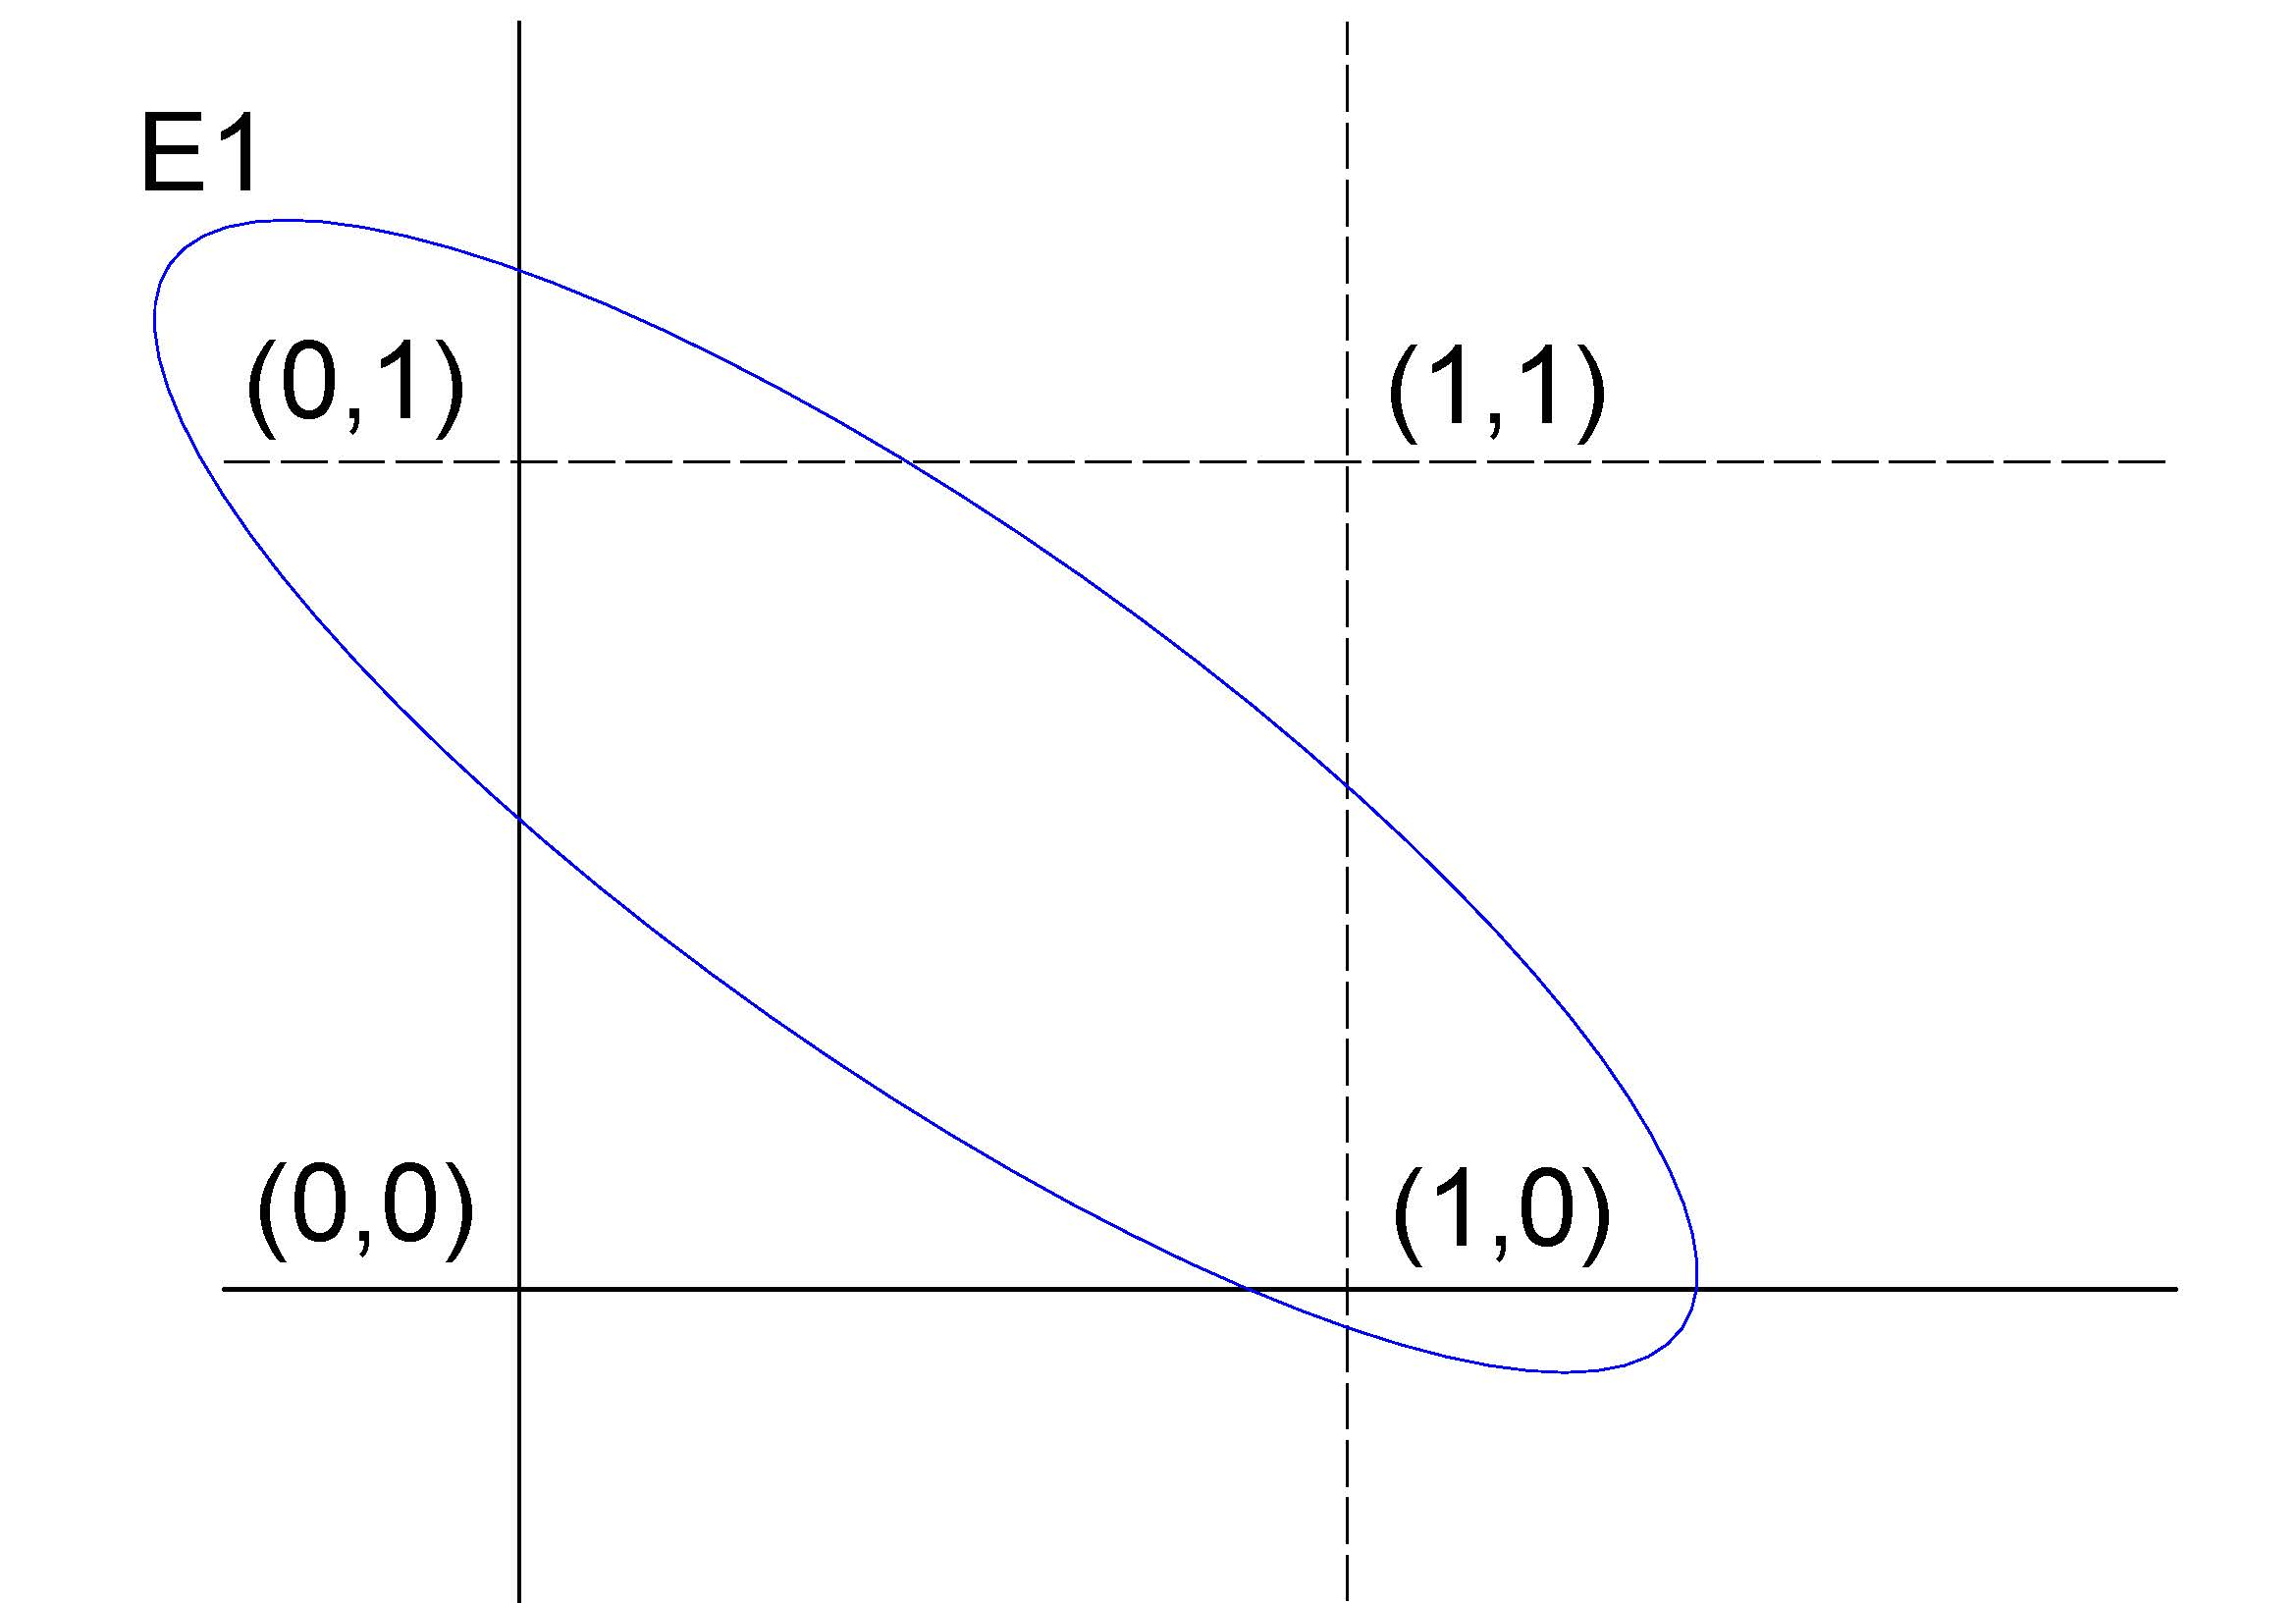
\includegraphics[width=0.5\linewidth]{images4/evento_grafico} 

}

\caption{Representação gráfico do espaço amostral do experimento aleatório e do evento de interesse definido}\label{fig:unnamed-chunk-55}
\end{figure}

\hfill\break

Admita agora um outro experimento aleatório, estabelecido como a soma dos valores das faces de dois dados (ou um dado laçado duas vezes) aleatoriamente lançados. O espaço amostral desse experimento aleatório será um conjunto formado por 11 elementos.

\hfill\break

\[
\Omega = \{\omega_{1}, \omega_{2}, \omega_{3}, \omega_{4}, \omega_{5}, \omega_{6}, \omega_{7}, \omega_{8}, \omega_{9}, \omega_{10}, \omega_{11}\}
\]

\hfill\break

onde:

\hfill\break

\begin{align*}
\omega_{1} & =  2\\
\omega_{2} & =  3\\
\omega_{3} & = 4\\
\omega_{4} & = 5\\
\omega_{5} & = 6\\
\omega_{6} & = 7 \\
\omega_{7} & = 8\\
\omega_{8} & = 9\\
\omega_{9} & = 10\\
\omega_{10} & = 11\\
\omega_{11} & = 12     
\end{align*}

\hfill\break

Cada um dos elementos que compõem o espaço amostral, a soma dos valores numéricos das faces no lançamento de um dado por duas vezes, poderá resultar de diferentes combinações de valores. A Tabela \ref{tab:table1} apresenta todas as combinações possíveis de serem obtidas, bem como as proporções em relação ao total para cada elemento do espaço amostral.

\hfill\break

\begin{longtable}[]{@{}
  >{\raggedright\arraybackslash}p{(\columnwidth - 6\tabcolsep) * \real{0.2381}}
  >{\raggedright\arraybackslash}p{(\columnwidth - 6\tabcolsep) * \real{0.4206}}
  >{\raggedright\arraybackslash}p{(\columnwidth - 6\tabcolsep) * \real{0.1746}}
  >{\raggedright\arraybackslash}p{(\columnwidth - 6\tabcolsep) * \real{0.1667}}@{}}
\caption{\label{tab:table1} Quadro dos possíveis resultados de um experimento aleatório: somas dos valores numéricos das faces no lançamento de um dado por duas vezes}\tabularnewline
\toprule\noalign{}
\begin{minipage}[b]{\linewidth}\raggedright
Soma
\end{minipage} & \begin{minipage}[b]{\linewidth}\raggedright
Possíveis combinações de resultados nos lançamentos
\end{minipage} & \begin{minipage}[b]{\linewidth}\raggedright
Frequência (\(n_{i}\))
\end{minipage} & \begin{minipage}[b]{\linewidth}\raggedright
Proporção (\(f_{i}\))
\end{minipage} \\
\midrule\noalign{}
\endfirsthead
\toprule\noalign{}
\begin{minipage}[b]{\linewidth}\raggedright
Soma
\end{minipage} & \begin{minipage}[b]{\linewidth}\raggedright
Possíveis combinações de resultados nos lançamentos
\end{minipage} & \begin{minipage}[b]{\linewidth}\raggedright
Frequência (\(n_{i}\))
\end{minipage} & \begin{minipage}[b]{\linewidth}\raggedright
Proporção (\(f_{i}\))
\end{minipage} \\
\midrule\noalign{}
\endhead
\bottomrule\noalign{}
\endlastfoot
& (primeiro,segundo) & & \\
2 & (1,1) & 1 & \(\frac{1}{36}\) \\
3 & (1,2); (2,1) & 2 & \(\frac{2}{36}\) \\
4 & (1,3); (2,2); (3,1) & 3 & \(\frac{3}{36}\) \\
5 & (1,4); (2,3); (3,2); (4,1) & 4 & \(\frac{4}{36}\) \\
6 & (1,5); (2,4); (3,3); (4,2); (5,1) & 5 & \(\frac{5}{36}\) \\
7 & (1,6); (2,5); (3,4); (4,3); (5,2); (6,1) & 6 & \(\frac{6}{36}\) \\
8 & (2,6); (3,5); (4,4); (5,3); (6,2) & 5 & \(\frac{5}{36}\) \\
9 & (3,6); (4,5); (5,4); (6,3) & 4 & \(\frac{4}{36}\) \\
10 & (4,6); (5,5); (6,4) & 3 & \(\frac{3}{36}\) \\
11 & (5,6); (6, 5) & 2 & \(\frac{2}{36}\) \\
12 & (6,6) & 1 & \(\frac{1}{36}\) \\
Totais & & 36 & \(\frac{1}{36}\) \\
\end{longtable}

\hfill\break

Se agora definimos nosso evento de interesse como sendo \textbf{obter uma soma ímpar}, nosso sucesso será verificado se ocorrer qualquer um desses elemetos do espaço amostral:

\hfill\break

\[
F=\{3;5;7;9;11\}
\]

\hfill\break

Nosso evento de interesse é um \emph{evento composto} pois é formado por 5 elementos do \emph{espaço amostral} \(\Omega\).

\hfill\break

Um evento de interesse \(G\) sobre o espaço amostral \(\Omega\) tal que

\hfill\break

\[
G=\Omega
\]

\hfill\break

expressa que qualquer um dos elementos de \(\Omega\) atende ao evento \(G\) e assim, a chance de ocorrência do evento \(G\) será absoluta. Esse tipo de evento é chamado de \textbf{evento certo}.

\hfill\break

Se definirmos em evento de interesse \(I\) com um resultado não pertencente aos possíveis resutados representados no \emph{espaço amostral} \(\Omega\), como, por exemplo, 13, ou então um conjunto vazio \(\varnothing\), esse evento será impossível de ocorrer. Esse tipo de evento é chamado de \textbf{evento impossível}.

\hfill\break

Desse modo temos diferentes tipos de eventos de inetersse:

\hfill\break

1- \emph{simples}: composto por apenas um elemento do espaço amostral;
2- \emph{composto}: composto por dois ou mais elementos do espaço amostral;
3- \emph{certo}: composto por todos os elementos do espaço amostral;\\
4- \emph{impossível}: composto por um elemento que não integra o espaço amostral.

\hfill\break

\hypertarget{operauxe7uxf5es-com-conjuntos-e-diagramas-de-venn}{%
\subsection{Operações com conjuntos e Diagramas de Venn}\label{operauxe7uxf5es-com-conjuntos-e-diagramas-de-venn}}

Em muitos dos problemas de probabilidade, o evento de interesse pode residir em \textbf{combinações de dois ou elementos} do conjunto que representa o espaço amostral. Uniões, interseções e complementos são alguns termos que, doravante, serão muito utilizados.

\hfill\break

\begin{figure}

{\centering \includegraphics[width=0.8\linewidth]{images4/venn} 

}

\caption{Diagramas de Venn}\label{fig:unnamed-chunk-56}
\end{figure}

\hfill\break

\hypertarget{uniuxe3o-a-cup-b}{%
\subsubsection{\texorpdfstring{União \(A \cup B\)}{União A \textbackslash cup B}}\label{uniuxe3o-a-cup-b}}

Sejam \(A\) e \(B\) dois subconjuntos finitos de um espaço amostral \(Omega=\{1,2,3,4,5,6\}\) tais que \(A=\{1,2,3\}\) e \(B=\{2,4,6\}\).

\hfill\break

Sua \emph{união}, representada por \(A \cup B\), é o subconjunto do espaço amostral \(\Omega\) que contém os elementos que pertençam \textbf{a \(A\), ou a \(B\) ou a ambos}. Desse modo, \(A \cup B =\{1,2,3,4,6\}\) e o Diagrama de Venn correspondente será:

\hfill\break

\begin{figure}

{\centering \includegraphics[width=0.8\linewidth]{images4/A_UN_B} 

}

\caption{União: $A \cup B$}\label{fig:unnamed-chunk-57}
\end{figure}

\hfill\break

\hypertarget{interseuxe7uxe3o-a-cap-b}{%
\subsubsection{\texorpdfstring{Interseção \(A \cap B\)}{Interseção A \textbackslash cap B}}\label{interseuxe7uxe3o-a-cap-b}}

Sua \emph{interseção}, representada por \(A \cap B\), é o subconjunto do espaço amostral \(\Omega\) que contém todos os elementos que pertencem \textbf{a ambos simultaneamente}. Desse modo, \(A \cap B =\{2\}\) e o Diagrama de Venn correspondente será:

\hfill\break

\begin{figure}

{\centering \includegraphics[width=0.8\linewidth]{images4/A_INTER_B} 

}

\caption{Interseção: $A \cap B$}\label{fig:unnamed-chunk-58}
\end{figure}

\hfill\break

Caso não exista nenhum elemento na interseção (ela é vazia) tem-se :

\[
A \cap B = \varnothing
\]

\hypertarget{complemmento-ac}{%
\subsubsection{\texorpdfstring{Complemmento \(A^{c}\)}{Complemmento A\^{}\{c\}}}\label{complemmento-ac}}

O \emph{complemento} de \(A\), representado por \(A^{c}\) (ou \(\stackrel{-}{A}\)), é o subconjunto do espaço amostral \(\Omega\) composto por todos os elementos que \textbf{não pertencem} a \(A\). Desse modo, \(\stackrel{-}{A} =\{4,5,6\}\) e o Diagrama de Venn correspondente será:

\hfill\break

\begin{figure}

{\centering \includegraphics[width=0.8\linewidth]{images4/COMP_A} 

}

\caption{Complementar  $A^{c}$}\label{fig:unnamed-chunk-59}
\end{figure}

\hfill\break

O \emph{complemento}\} de \(B\), representado por \(B^{c}\) (ou \(\stackrel{-}{B}\)), é o subconjunto do espaço amostral \(\Omega\) composto por todos os elementos que \textbf{não pertencem} a \(B\). Desse modo, \(\stackrel{-}{B} =\{1,3,5\}\) e o Diagrama de Venn correspondente será :

\hfill\break

\begin{figure}

{\centering \includegraphics[width=0.8\linewidth]{images4/COMP_B} 

}

\caption{Complementar de B}\label{fig:unnamed-chunk-60}
\end{figure}

\hypertarget{eventos-equiprovuxe1veis-e-nuxe3o-equiprovuxe1veis}{%
\subsection{Eventos equiprováveis e não equiprováveis}\label{eventos-equiprovuxe1veis-e-nuxe3o-equiprovuxe1veis}}

\hfill\break

Se todos os elementos que compõem um espaço amostral finito de um experimento aleatório possuem a mesma probabilidade de ocorrência é dito que esse espaço amostral é \textbf{uniforme} ou que seus elementos são \textbf{equiprováveis}.

\hfill\break

No experimento de se lançar um dado e anotar o valor numérico de sua face todos os possíveis resultados apresentam a mesma probabilidade: \(\frac{1}{6}\).

\hfill\break

Já no experimento de se lançar dois dados e se anotar a soma dos valores numéricos de suas faces as probabilidades são diferentes.

\hfill\break

Um significativo resultado é que a soma das probabilidades associadas a cada um desses possíveis resultados é um (1) (antecipando um dos postulados do conceito axiomático de probabilidade).

\hypertarget{eventos-independentes}{%
\subsection{Eventos independentes}\label{eventos-independentes}}

Quando a possibilidade de ocorrência de um evento de interesse (sucesso) em um determinado exeprimento aleatório não é afetada pelo resultado \textbf{prévio} de outro diz-se que esses dois eventos são \textbf{independentes}\}. Caso contrário são ditos dependentes ou condicionados. Mais adiante esse conceito será introduzido de um modo mais detalhado.

\hypertarget{eventos-mutuamente-exclusivos}{%
\subsection{Eventos mutuamente exclusivos}\label{eventos-mutuamente-exclusivos}}

Dois eventos que nunca poderão ocorrer simultaneamente são ditos mutuamente exclusivos. No experimento do lançamento da moeda por uma vez, nunca observaremos simultaneamente os eventos: \(E=\{(Cara)\}\) \textbf{e} \(F=\{(Coroa)\}\) e assim sua interseção é vazia:

\hfill\break

\[
E \cap F = \varnothing 
\]

\hfill\break

E por essa razão, se chamarmos de \(P(E)\) e \(P(F)\) as probabilidades de ocorrência desses reultados veremos que :

\[
P(E) \cap P(F) = 0
\]

\hypertarget{eventos-complementares}{%
\subsection{Eventos complementares}\label{eventos-complementares}}

Definido um evento de interesse qualquer pode-se observar apenas dois resultados: \textbf{ocorrer} ou \textbf{não} o sucesso; ou seja, um ou outro deverá forçosamente ocorrer.\\

Chama-se de evento complementar (\(E^{c}\) ou \(\stackrel{-}{E}\)) a um evento (\(E\)), aquele cuja probabilidade de sucesso seja:

\[
P(E^{c}) = 1 - P(E)
\]

Se a probabilidade de sucesso de que ele ocorra for \(P(E)=p\) e a de que ele não ocorra for \(P(E^{c}= q)\) vê-se que a soma dessas quantidades deverá ser \(p + q =1\) (novamente antecipando um dos postulados do conceito axiomático de probabilidade).

\hypertarget{probabilidade}{%
\section{Probabilidade}\label{probabilidade}}

\hypertarget{introduuxe7uxe3o-histuxf3rica}{%
\subsection{Introdução histórica}\label{introduuxe7uxe3o-histuxf3rica}}

De acordo com alguns historiadores, a Teoria das probabilidades teve início como um ramo da Matemática com as célebres cartas entre Blaise Pascal (1623-1662) e Pierre de Fermat (1607-1665), após uma consulta feita por um nobre cavaleiro (Antoine Gombaud, o \emph{Chevalier de Méré}) a Pascal, relacionadas a como repartir um montante apostado em um jogo de dados caso ele tenha que ser interrompido antes de sua conclusão. Todavia o estudo não formal remonta a alguns séculos atrás.

\hfill\break

Probabilidade tem sido definida como sendo o estudo da frequência de aparição de um fenômeno em relação a todas as suas possíveis alternativas; ou seja, seu objeto é o estudo das possibilidades dos fenômenos aleatórios. O estudo das probabilidades possui, digamos assim, duas raízes históricas:

\hfill\break

1- a solução de problemas relacionados a jogos; e,\\
2- a análise estatística de dados atuariais.

\hfill\break

\begin{figure}

{\centering \includegraphics[width=0.8\linewidth]{images4/astralagus} 

}

\caption{Astralagus (um dos ossos que compõem o calcanhar, usado no Egito antigo como um dado rudimentar)}\label{fig:unnamed-chunk-61}
\end{figure}

\hypertarget{conceito-cluxe1ssico-ou-a-priori}{%
\subsection{\texorpdfstring{Conceito clássico ou \emph{a priori}}{Conceito clássico ou a priori}}\label{conceito-cluxe1ssico-ou-a-priori}}

Sob uma visão intuitiva, a probabilidade como uma medida da informação que temos sobre a possibilidade de ocorrência de um evento aleatório, pode ser definida como a medida numérica expressa em termos relativos (percentuais), obtida pela razão (proporção) entre o número de eventos favoráveis (sucessos) pelo número total de eventos prováveis no experimento (espaço amostral).

\hfill\break

Esse conceito de probabilidade é denominado \emph{clássico} ou \emph{a priori}, baseado em um conhecimento prévio ou uma crença subjetiva sobre a probabilidade de um evento ocorrer.

\hfill\break

Por exemplo, um jogador de cartas pode ter uma crença a priori de que a probabilidade de uma carta ser um ás é de 1 em 13, independentemente do número de baralhos no jogo

\hfill\break

A distribuição de frequências é um instrumento importante para a análise da variabilidade de experimentos aleatórios e, em particular, as frequências relativas são estimativas das probabilidades.

\hfill\break

\[
P(E)= \frac{\text{número de resultados de interesse (sucessos)}}{\text{número total de resultados possíveis no espaço amostral}}
\]

\hfill\break

Com o estabelecimento de suposições adequadas, um modelo teórico de probabilidade pode ser estabelecido sem a observação \emph{a priori} dos resultados de experimento aleatório, reproduzindo de modo razoável a distribuição das frequências quando o experimento é diretamente observado.

\hfill\break

Consideremos o exemplo do experimento que consiste em se lançar um dado e observar o valor numérico de sua face. As suposições que deveriam ser estabelecidas \emph{a priori} são:

\hfill\break

\begin{itemize}
\tightlist
\item
  só pode ocorrer uma das seis faces; e,
\item
  o dado utilizado não possui viés algum (não favorece face alguma).
\end{itemize}

\hfill\break

Como todos os \(N\) resultados do espaço amostral apresentam uma \textbf{mesma probabilidade} de ocorrência, então a proporção teórica de ocorrência de qualquer um desse resultados poderá ser apresentado na forma vista na na forma vista na Tabela \ref{tab:table2}.

\hfill\break

\[
P(E)= \frac{1}{N}
\]

\hfill\break

\begin{longtable}[]{@{}
  >{\raggedright\arraybackslash}p{(\columnwidth - 14\tabcolsep) * \real{0.1418}}
  >{\raggedright\arraybackslash}p{(\columnwidth - 14\tabcolsep) * \real{0.1348}}
  >{\raggedright\arraybackslash}p{(\columnwidth - 14\tabcolsep) * \real{0.1348}}
  >{\raggedright\arraybackslash}p{(\columnwidth - 14\tabcolsep) * \real{0.1348}}
  >{\raggedright\arraybackslash}p{(\columnwidth - 14\tabcolsep) * \real{0.1348}}
  >{\raggedright\arraybackslash}p{(\columnwidth - 14\tabcolsep) * \real{0.1348}}
  >{\raggedright\arraybackslash}p{(\columnwidth - 14\tabcolsep) * \real{0.1348}}
  >{\raggedright\arraybackslash}p{(\columnwidth - 14\tabcolsep) * \real{0.0496}}@{}}
\caption{\label{tab:table2} Distribuição das proporções teóricas do um experimento aleatório: lançamento de um dado}\tabularnewline
\toprule\noalign{}
\begin{minipage}[b]{\linewidth}\raggedright
Face
\end{minipage} & \begin{minipage}[b]{\linewidth}\raggedright
1
\end{minipage} & \begin{minipage}[b]{\linewidth}\raggedright
2
\end{minipage} & \begin{minipage}[b]{\linewidth}\raggedright
3
\end{minipage} & \begin{minipage}[b]{\linewidth}\raggedright
4
\end{minipage} & \begin{minipage}[b]{\linewidth}\raggedright
5
\end{minipage} & \begin{minipage}[b]{\linewidth}\raggedright
6
\end{minipage} & \begin{minipage}[b]{\linewidth}\raggedright
Total
\end{minipage} \\
\midrule\noalign{}
\endfirsthead
\toprule\noalign{}
\begin{minipage}[b]{\linewidth}\raggedright
Face
\end{minipage} & \begin{minipage}[b]{\linewidth}\raggedright
1
\end{minipage} & \begin{minipage}[b]{\linewidth}\raggedright
2
\end{minipage} & \begin{minipage}[b]{\linewidth}\raggedright
3
\end{minipage} & \begin{minipage}[b]{\linewidth}\raggedright
4
\end{minipage} & \begin{minipage}[b]{\linewidth}\raggedright
5
\end{minipage} & \begin{minipage}[b]{\linewidth}\raggedright
6
\end{minipage} & \begin{minipage}[b]{\linewidth}\raggedright
Total
\end{minipage} \\
\midrule\noalign{}
\endhead
\bottomrule\noalign{}
\endlastfoot
Proporção teórica & \(\frac{1}{6}\) & \(\frac{1}{6}\) & \(\frac{1}{6}\) & \(\frac{1}{6}\) & \(\frac{1}{6}\) & \(\frac{1}{6}\) & 1 \\
\end{longtable}

\hfill\break

Sendo equiprováveis todos os elementos do espaço amostral, todos terão a mesma probabilidade de ocorrência que será:

\hfill\break

\begin{align*}
P(E) = & \frac{1}{N} \\
     = &  \frac{1}{6} \\
     = & \frac{1}{6}    
\end{align*}

\hfill\break

Por essa razão sabe-se, \emph{a priori} a probabilidade de ocorrência de qualquer evento ao se realizar esse tipo de experimento aleatório uma única vez.

\hfill\break

\hypertarget{conceito-frequentista-ou-a-posteriori}{%
\subsection{\texorpdfstring{Conceito frequentista ou \emph{a posteriori}}{Conceito frequentista ou a posteriori}}\label{conceito-frequentista-ou-a-posteriori}}

\hfill\break

Todavia, se realizarmos o experimento aleatório anterior apenas algumas, tal regularidade poderá não ser comprovada: as frequências observadas (as quantidades obtidas para cada um dos valores numéricos das faces) apresentarão uma \textbf{grande irregularidade} diferindo das frequência teóricas definidas.

\hfill\break

Observa-se que os resultados das frequências observadas irá se estabilizar, aproximando-se das frequências teóricas, à medida que se repete esse experimento um número suficientemente grande de vezes.

\hfill\break

A definição frequencial (\emph{a posteriori}):

\hfill\break

1- refere-se à probabilidade empírica observada \emph{a posteriori};
2- tem por objetivo estabelecer um modelo adequado à interpretação de alguns tipos de experimentos aleatórios; e,
3- é a base para se formular um modelo teórico de distribuição de probabilidades como os que serão abordados mais adiante.

\hfill\break

Ao se repetir o experimento aleatório um grande número de vezes ( \(n\) tendendo a infinitas vezes), a quantidade de vezes que um determinado resultado foi verificado dividida por o número de repetições realizadas (\(n\)) irá se aproximar de sua proporção teórica.

\hfill\break

É o que se denomina como \emph{regularidade estatística dos resultados} por essa propriedade não mais se necessita que os eventos sejam \emph{equiprováveis}.

\hfill\break

\[
P\left(E\right)=\underset{n\to \infty }{lim}{\frac{F(E)}{n}}
\]

\hfill\break

onde:

\hfill\break

\begin{itemize}
\tightlist
\item
  \(P(E)\) é a probabilidade de ocorrência do evento \(E\);\\
\item
  \(F(E)\) é a frequência observada do evento \(E\) (o número de vezes que ele ocorre em \emph{n} repetições); e,\\
\item
  \(n\) é o número de repetições do experimento.
\end{itemize}

\hfill\break

\hfill\break

\hypertarget{conceito-axiomuxe1tico}{%
\subsection{Conceito axiomático}\label{conceito-axiomuxe1tico}}

\hfill\break

Esta abordagem é baseada em um conjunto de axiomas matemáticos que definem as propriedades básicas de probabilidades. A probabilidade é definida como uma função de conjuntos que atribui a cada conjunto de eventos um número entre 0 e 1, satisfazendo os axiomas matemáticos de probabilidade. Essa abordagem permite que as probabilidades sejam definidas formalmente e usadas para cálculos matemáticos.

\hfill\break

\begin{quote}
Um \emph{axioma} é uma premissa considerada necessariamente evidente e verdadeira, fundamento de uma demonstração, porém ela mesma indemonstrável, originada, segundo a tradição racionalista, de princípios inatos da consciência ou, segundo os empiristas, de generalizações da observação empírica.
\end{quote}

\hfill\break

Admita \(P\) uma função que opera sobre o espaço \(\Omega\); isto é, uma função que associa uma quantidade \(P(\Omega)\) a cada elemento \(\omega\) \(\in\) \(\Omega\).

\hfill\break

\begin{figure}

{\centering \includegraphics[width=0.8\linewidth]{images4/funcao_probabilidade} 

}

\caption{Representação gráfica da função $P(\Omega)$}\label{fig:unnamed-chunk-62}
\end{figure}

\hfill\break

Essa função \(P\) será uma \textbf{função de probabilidade} se, e somente se, satisfizer a \textbf{três axiomas} (postulados: conceitos iniciais necessários à construção ou aceitação de uma teoria) estabelecidos por Andrey Kolmogorov (1933).

\hfill\break

\begin{figure}

{\centering \includegraphics[width=0.4\linewidth]{images4/kolmogorov} 

}

\caption{Andrey Nikolaevich Kolmogorov  (1903-1987)}\label{fig:unnamed-chunk-63}
\end{figure}

\hfill\break

Kolmogoroff afirmou que uma \emph{Teoria das probabilidades} poderia ser desenvolvida a partir de \emph{axiomas}, da
mesma forma que a geometria e a álgebra, e a considerou como caso especial da \emph{Teoria da medida e integração} desenvolvida por Lebesgue, Borel e Fréchet. Ele estabeleceu como postulados as propriedades comuns das noções de probabilidade clássica e frequentista que, desta forma, viraram casos particulares da definição axiomática.

\hfill\break

\hypertarget{postulado-do-intervalo}{%
\subsubsection{Postulado do intervalo}\label{postulado-do-intervalo}}

A probabilidade de qualquer \(E\) \textbf{é um número real entre 0 e 1} (pode-se entender isso como uma convenção, onde então se estabelece a medida da probabilidade é um número positivo e que qualquer evento pode ter probabilidade de, no máximo, 1). Esse postulado está plenamente de acordo com a interpretação frequentista de probabilidade.

\hfill\break

\[
0 \hspace{0.5cm} \le P(\Omega) \hspace{0.5cm} \le 1
\]

\hfill\break

\hypertarget{postulado-da-certeza}{%
\subsubsection{Postulado da certeza}\label{postulado-da-certeza}}

O segundo postulado refere-se à probabilidade do \textbf{evento certo} ser igua a 1. No que diz respeito à interpretação frequentista, uma probabilidade de 1 implica que o evento em questão ocorrerá 100\% do tempo ou, em outras palavras, \textbf{que é certo que ele ocorra} (como, p.~exemplo, um experimento aleatório de se lançar dois dados e somar o valor de suas faces o evento certo poderia ser definido como observar uym valor menor que 13 ou maior que 2)

\hfill\break

\[
P(\Omega) = 1
\]

\hfill\break

\hypertarget{postulado-da-aditividade-para-eventos-mutuamente-exclusivos}{%
\subsubsection{Postulado da aditividade para eventos mutuamente exclusivos}\label{postulado-da-aditividade-para-eventos-mutuamente-exclusivos}}

\[
P\left(\bigcup _{n=1}^{\infty }{\omega}_{n}\right)=\sum _{n=1}^{\infty }P\left({\omega}_{n}\right)
\]

\hfill\break

para qualquer sequência de eventos \textbf{mutuamente exclusivos} \(\{\omega_{1}, \omega_{2}, \omega_{3}, ..., \omega_{n}, ...\}\) (isto é, tal que \(\omega_{i} \cap \omega_{j} \varnothing\) se \(i \neq j\))

\hfill\break

Tomando o terceiro postulado no caso mais simples, isto é, para \textbf{dois} eventos mutuamente exclusivos \(\omega_{1}\) e \(\omega_{2}\), pode ser facilmente visto que é satisfeito pela interpretação frequentista.

\hfill\break

Se um evento ocorrer, digamos, 28\% das vezes, outro evento ocorrerá 39\%, \textbf{e os dois eventos não podem ocorrer ao mesmo tempo (ou seja, são mutuamente exclusivos)}, então um \textbf{ou outro} evento\} ocorrerão em 28 + 39 = 67\% das vezes. Assim, o terceiro postulado é satisfeito, e o mesmo tipo de argumento se aplica quando há mais de dois eventos mutuamente exclusivos.

\hfill\break

\textbf{Recapitulando}

\hfill\break

1- foi definido o conceito de \textbf{experimento aleatório} como sendo aquele cujos resultados não podem ser determinados com certeza antes de sua realização;\\
2- foi definido o conceito de \textbf{espaço amostral} de um experimento aleatório como sendo o conjunto de \textbf{todos os possíveis resultados} que ele pode apresentar;\\
3- foi definido que um \textbf{evento de interesse} é um subconjunto do espaço amostral no qual estamos particularmente interessados;\\
4- foi definida uma \textbf{função} que tem como domínio o espaço amostral e associa uma quantidade (entre \textbf{0} e \textbf{1}) a \textbf{cada elemento} do espaço amostral; e, por fim,\\
5- estabelecemos que \textbf{se} essa função atende a \textbf{três postulados} então ela será uma \textbf{medida da probabilidade} de ocorrẽncia de cada evento do espaço amostral em questão.

\hfill\break

Assim, quando uma função \(P\) associa uma quantidade \(P(\Omega)\) a um evento \(\omega\) e \(P(\Omega)\) atende aos três axiomas anteriormente estabelecidos, diz-se que que ela é a \textbf{função de probabilidade} de \(\Omega\).

\hfill\break

\hypertarget{probabilidade-da-uniuxe3o-de-eventos}{%
\subsection{Probabilidade da união de eventos}\label{probabilidade-da-uniuxe3o-de-eventos}}

Considerem agora a Tabela \ref{tab:table3} de dupla entrada onde vemos a distribuição de alunos conforme seu sexo e o curso escolhido:

\hfill\break

\begin{longtable}[]{@{}
  >{\raggedright\arraybackslash}p{(\columnwidth - 6\tabcolsep) * \real{0.3425}}
  >{\raggedright\arraybackslash}p{(\columnwidth - 6\tabcolsep) * \real{0.3699}}
  >{\raggedright\arraybackslash}p{(\columnwidth - 6\tabcolsep) * \real{0.1918}}
  >{\raggedright\arraybackslash}p{(\columnwidth - 6\tabcolsep) * \real{0.0959}}@{}}
\caption{\label{tab:table3} Distribuição da quantidade de alunos segundo seu sexo e curso escolhido}\tabularnewline
\toprule\noalign{}
\begin{minipage}[b]{\linewidth}\raggedright
Curso
\end{minipage} & \begin{minipage}[b]{\linewidth}\raggedright
Sexo
\end{minipage} & \begin{minipage}[b]{\linewidth}\raggedright
\end{minipage} & \begin{minipage}[b]{\linewidth}\raggedright
\end{minipage} \\
\midrule\noalign{}
\endfirsthead
\toprule\noalign{}
\begin{minipage}[b]{\linewidth}\raggedright
Curso
\end{minipage} & \begin{minipage}[b]{\linewidth}\raggedright
Sexo
\end{minipage} & \begin{minipage}[b]{\linewidth}\raggedright
\end{minipage} & \begin{minipage}[b]{\linewidth}\raggedright
\end{minipage} \\
\midrule\noalign{}
\endhead
\bottomrule\noalign{}
\endlastfoot
& Masculino (M) & Feminino (F) & Total \\
Matemática pura (M) & 70 & 40 & 110 \\
Matemática aplicada (A) & 15 & 15 & 30 \\
Estatística (E) & 10 & 20 & 30 \\
Computação (C) & 20 & 10 & 30 \\
Total & 115 & 85 & 200 \\
\end{longtable}

\hfill\break

Essa tabela nos possibilita calcular a probabilidade de ocorrência de diversos eventos de interesse que desejemos estabelecer.

\hfill\break

\begin{quote}
Exemplo: seja o experimento aleatório de se escolher, aleatoriamente, um estudante qualquer desses quatro cursos. Assim, se definimos nosso evento de interesse \(M\) como sendo \textbf{M:sexo masculino}, a probabilidade de sucesso (que o indivíduo sorteado aleatoriamente seja do sexo masculino) será:
\end{quote}

\hfill\break

\[
P(M) = \frac{115}{200}
\]

\hfill\break

\begin{quote}
Exemplo: se nosso evento de interesse \(A\) como sendo \textbf{\(A:\) curso de matemática aplicada} , a probabilidade de sucesso (que o indivíduo sorteado aleatoriamente seja do curso de matemática aplicada será):
\end{quote}

\[
P(A) = \frac{30}{200}
\]

\hfill\break

A partir dos eventos de interesse anteriormente estabelecidos, podemos definir outros eventos na forma de uniões (\(\cup\)) e interseções (\(\cap\)):

\hfill\break

\begin{itemize}
\tightlist
\item
  uma união entre os dois eventos de interesse anteriores \(A\) e \(M\) é representada por \(A \cup M\) (alternativamente lê-se também \textbf{ou}) e representa um evento onde \textbf{pelo menos} um dos dois eventos básicos pode ocorrer: \textbf{ou} \(A\), \textbf{ou} \(M\) \textbf{ou ambos}; e,\\
\item
  uma interseção dos dois eventos de interesse anteriores \(A\) e \(M\) é representada por \(A \cap M\) (alternativamente lê-se também \textbf{e}) e representa um evento onde \textbf{os dois eventos} básicos devem ocorrer: \(A\) \textbf{e} \(M\).
\end{itemize}

\hfill\break

\begin{quote}
Exemplo: se definimos nosso evento de interesse (\(P(A \cap M)\)) como sendo \textbf{sexo masculino e cursando matemática aplicada}. Facilmente podemos visualizar na Tabela \ref{tab:table3} que apenas 15 alunos do curso do evento de interesse (matemática aplicada) são do sexo do segundo evento de interesse (masculino), em relação a todo espaço amostral e assim:
\end{quote}

\hfill\break

\[
P(A \cap M) = \frac{15}{200}
\].

\hfill\break

\begin{quote}
Exemplo: consideremos agora o evento de interesse (\(P(A \cup M)\)) como sendo \textbf{sexo masculino ou cursando matemática aplicada}.
\end{quote}

\hfill\break

Na Tabela \ref{tab:table3} temos as duas probabilidades \textbf{marginais}:

\hfill\break

\begin{enumerate}
\def\labelenumi{\arabic{enumi}.}
\tightlist
\item
  \(P(A)=\frac{30}{200}\) (curso: matemática aplicada); e,
  2- \(P(M)=\frac{115}{200}\) (sexo masc).
\end{enumerate}

\hfill\break

Poderíamos intuir equivocadamente que:

\hfill\break

\[
P(A \cup M) = P(A) + P(M) = \frac{30}{200} + \frac{115}{200} = \frac{145}{200}
\]

\hfill\break

Tal raciocínio é errado pois iria considerar por \textbf{duas vezes} os alunos do \textbf{sexo masculino}. Uma fração da quantidade global (115) de alunos do \textbf{sexo masculino} já considera aqueles que estão matriculados no curso de \textbf{matemática aplicada} (15). É preciso \textbf{subtrair} da soma das probabilidades marginais essa \textbf{parcela em comum} que é a interseção dos dois eventos básicos.

A resposta correta será:

\[
P(A \cup M) = P(A) + P(M) - P(A \cap M) = \frac{30}{200} + \frac{115}{200} -\frac{15}{200} = \frac{130}{200}
\].

\hfill\break

Portanto, para quaisquer eventos de intersse \(A\) e \(B\), podemos estabelecer uma \textbf{regra geral da pobabilidade da união de dois eventos quaiquer} como:

\hfill\break

\[
P(A \cup B) = P(A) + P(B) - P(A \cap B)
\]

\hfill\break

Se \(A\) e \(B\) forem \textbf{mutuamente exclusivos}, a interseção entre eles será vazia (\(A \cap B =\varnothing\)) e, assim, essa probabiidade é zero. Nessa situação, a probabilidade de \(P(A \cup B)\) fica reduzida a uma \textbf{regra particular para a adição de probabilidades de eventos mutuamente exclusivos}:

\hfill\break

\[
P(A \cup B) = P(A) + P(B)
\]

\hfill\break

\begin{quote}
Exemplo: Seja o experimento aleatório de se lançar um dado (com seis faces) e observar o valor numérico da face que ficar exposta. Qual a probabilidade de se observar os valores \(1\) \textbf{ou} \(4\)?
\end{quote}

\hfill\break

Definindo os eventos de interesse:

\hfill\break

1- \(E_{1}=\text{sair face 1}\) (\(P(E_{1})=\frac{1}{6}\)); e,\\
2- \(E_{4}=\text{sair face 4}\) (\(P(E_{4})=\frac{1}{6}\)).

\hfill\break

Pede-se \(P(E_{1} \cup E_{4})\).

\hfill\break

Como \(E_{1}\) e \(E_{4}\) são *eventos mutuamente exclusivos**: \(E_{1} \cap E_{4}=\varnothing\) (portanto a probabilidade é zero), então \(P(E_{1} \cup E_{4}) = P(E_{1}) + P(E_{4}) = \frac{1}{6} + \frac{1}{6}= \frac{1}{3}\).

\hfill\break

\begin{quote}
Exemplo: Uma população é composta por 20 pessoas que consomem o produto \textbf{A}, 30 pessoas que consomem o produto \textbf{B} e 50 pessoas que consomem o produto \textbf{C} . Um pesquisador de mercado seleciona aleatoriamente uma pessoa desta população. \textbf{Sabendo que uma pessoa não consome mais de um produto ao mesmo tempo}, qual a probabilidade de ter sido selecionada uma pessoa que consome os produtos \textbf{A ou C}?
\end{quote}

\hfill\break

Solução:

\hfill\break

Definindo os eventos de interesse e as probabilidades associadas:

\hfill\break

1- \(E_{A}=\text{consumidor do produto A}\): \(P(E_{A}=\frac{20}{100}\));\\
2- \(E_{B}=\text{consumidor do produto B}\): \(P(E_{B}=\frac{30}{100}\)); e,\\
3- \(E_{C}=\text{consumidor do produto C}\): \(P(E_{C}=\frac{50}{100}\)).

\hfill\break

Pela regra geral da probabilidade da união de dois eventos quaiquer sabemos que:

\hfill\break

\[
P(E_{A} \cup E_{C}) = P(E_{A}) + P(E_{C}) - P(E_{A} \cap E_{C})
\]

\hfill\break

Como foi estabelecido no enunciado que uma pessoa \textbf{não} consome mais de um produto ao mesmo tempo (esses eventos são, portanto, \textbf{mutuamente exclusivos}: \(E_{A} \cap E_{C}=\varnothing\)) a probabilidade pedida será:

\hfill\break

\begin{align*}
P(E_{A} \cup E_{C}) & = P(E_{A}) + P(E_{C}) - P(E_{A} \cap E_{C}) \\
                    & = \frac{20}{10} + \frac{50}{100} - 0 \\
                    & =  \frac{70}{100} \\
                    & =  0,70    
\end{align*}

\hfill\break

\hypertarget{probabilidade-de-eventos-condicionados}{%
\subsection{Probabilidade de eventos condicionados}\label{probabilidade-de-eventos-condicionados}}

Dois eventos \(A\) e \(B\) de um experimento aleatório qualquer são ditos \textbf{condicionados} quando a ocorrência prévia de um deles impõe \textbf{uma restrição} no espaço amostral do segundo.

\hfill\break

A \textbf{probabilidade} de um evento qualquer \(A\) \textbf{condicionada} a um segundo evento \(B\) é representada como \(P(A|B)\). A \emph{barra} verical pode ser ``lida'' adotando-se termos correlatos que facilitam o entendimento da relação existente, tais como :

\hfill\break

\begin{itemize}
\tightlist
\item
  probabilidade de \(A\) \textbf{posto que} ocorreo \(B\);
\item
  probabilidade de \(A\) \textbf{admitindo-se} que ocorreu \(B\);
\item
  probabilidade de \(A\) \textbf{considerando-se} que ocorreu \(B\),
\end{itemize}

\hfill\break

e seu cálculo é feito pela \textbf{regra geral da probabilidade de dois eventos condicionados}:

\hfill\break

\begin{align*}
P(A|B) & = \frac{ P(A\cap B)}{ P(B)} \\
P(B|A) & = \frac{ P(B\cap A)}{ P(A)}
\end{align*}

\hfill\break

sendo \(P(B)>0\) e \(P(A)>0\) nas expressões acima.

\hfill\break

De modo geral, admita que os eventos \(E_{1}\), \(E_{2}\),\ldots,\(E_{n}\) formam uma partição do espaço amostral.

\hfill\break

Os eventos não têm interseções entre si e a união destes é igual ao espaço amostral e seja \(A\) um evento qualquer desse espaço.

\hfill\break

Então a probabilidade de ocorrência desse evento será dada por:

\hfill\break

\begin{align*}
P(A) & = P(A \cap E_{1}) +  P(A \cap E_{2}) + \dots + P(A \cap E_{n}) \\
     & = P(E_{1}) \times P(A|E_{1}) + P(E_{2}) \times P(A|E_{2}) + \dots + \\
     & P(E_{n}) \times P(A|E_{n})\\
\end{align*}

\hfill\break

\begin{quote}
Exemplo: Consideremos a Tabela \ref{tab:table3} que apresenta informações cruzadas do sexo dos alunos e seus respectivos cursos. Vamos definir os eventos \textbf{Fem:sexo feminino} e \textbf{Est: cursar estatística}. Como calcular a probabilidade condicionada de nosso evento de interesse \textbf{P(Fem\textbar Est)} (a probabilidade de um aluno aleatoriamente escolhido ser do sexo \textbf{feminino}, \textbf{dado} que ele cursa \textbf{estatística})?
\end{quote}

\hfill\break

\begin{align*}
P(Fem|Est) & = \frac{ P(Fem \cap Est)}{ P(Est)} \\
           & = \frac{20}{30} = \frac{2}{3}    
\end{align*}

\hfill\break

Esse cálculo é facilmente entendido observando-se as celulas da distribuição de frequências na Tabela \ref{tab:table3}.

\hfill\break

\begin{quote}
Exemplo: Considerem a Tabela \ref{tab:table4} que relaciona a ida à praia de uma certa pessoa às condições climáticas do dia.
\end{quote}

\hfill\break

\begin{longtable}[]{@{}lllllllllll@{}}
\caption{\label{tab:table4} Condicionamento de passeios à praia em relação às condições climáticas observadas}\tabularnewline
\toprule\noalign{}
Dia & 1 & 2 & 3 & 4 & 5 & 6 & 7 & 8 & 9 & 10 \\
\midrule\noalign{}
\endfirsthead
\toprule\noalign{}
Dia & 1 & 2 & 3 & 4 & 5 & 6 & 7 & 8 & 9 & 10 \\
\midrule\noalign{}
\endhead
\bottomrule\noalign{}
\endlastfoot
Foi à praia? & N & S & N & S & S & S & N & N & S & S \\
Fez sol? & N & S & N & S & N & S & S & N & S & S \\
\end{longtable}

\hfill\break

Baseado nos dados coletados responda:

\hfill\break

1- Qual a probabilidade dessa pessoa ir à praia?\\
2- Sabendo-se que fez Sol, qual a probabilidade dessa pessoa ir à praia?\\
3- Os eventos \textbf{ir à praia} e \textbf{fazer Sol} são independentes ou condicionados?

\hfill\break

Da Tabela \ref{tab:table4} extraímos as seguintes probabilidades:

\hfill\break

\begin{align*}
P(IP) & = \frac{6}{10}= 0,60 \\
P(FS) & = \frac{6}{10}= 0,60 \\
P(IP \cap FS) & = \frac{5}{10} \\
    & = 0,50 
\end{align*}

\hfill\break

A partir delas podemos calcular a seguinte probabilidade condicionada:

\hfill\break

\begin{align*}
P(IP|FS) & = \frac{ P(IP \cap F)}{ P(FS)} \\
       & = \frac{5}{6} \\
       & = 0,83     
\end{align*}

\hfill\break

A probabilidade dessa pessoa ir à praia (\(P(IP)\)) é 0,60; \textbf{mas} quando faz Sol a probabilidade (\(P(IP|FS)\)) dela aumenta para 0,83.

\hfill\break

Assim, os eventos \(IP\) e \(FS\) são condicionados: essa pessoa vai à praia 60\% dos dias analisados; mas, \textbf{quando faz sol}, ela vai em 83\% dos dias (a presença de Sol altera a probabilidade dela ir à praia).

\hfill\break

\begin{quote}
Exemplo: Em uma cidade existem 15.000 usuários de telefonia, dos quais 10.000 possuem telefones fixos, 8.000 telefones móveis e 3.000 telefones fixos e móveis. Seja o experimento aleatório de uma operadora de telefone móvel selecionar uma pessoa dessa cidade para oferecer uma promoção do tipo ``Fale Grátis de seu Móvel para seu Fixo''.
\end{quote}

\hfill\break

Responda:

\hfill\break

1- Sorteando-se aleatoriamente um cliente dessa operadora, se soubermos antecipadamente que ele tem telefone móvel, qual a probabilidade de esse cliente tenha telefone fixo também?\\
2- Sabendo-se que ele tem telefone fixo, qual a probabilidade de ele tenha telefone móvel também?

\hfill\break

O espaço amostral de todos esses possíveis eventos pode ser ilustrado pelo diagrama de Venn abaixo:

\hfill\break

\begin{figure}

{\centering \includegraphics[width=0.5\linewidth]{images4/exercicio} 

}

\caption{Diagrama de Venn do espaço amostral}\label{fig:venn}
\end{figure}

\hfill\break

Do diagrama apresentado na Figura\ref{fig:venn} podemos extrair imediatamente as probabilidades pedidas:

\hfill\break

\begin{itemize}
\tightlist
\item
  \(P(F|M)\) (probabilidade de ter uma linha fixa sabendo que possui um telefone móvel); e,
\item
  \(P(M|F)\) (probabilidade de ter uma linha móvel sabendo que possui um telefone fixo):
\end{itemize}

\hfill\break

\begin{align*}
P(F|M) & = \frac{n(MF)}{n(M)}\\
       & =\frac{3000}{8000}\\
       & = 0,375 
\end{align*}\\

e

\hfill\break

\begin{align*}
P(M|F) & = \frac{n(MF)}{n(F)} \\
       & =\frac{3000}{10000} \\
       & = 0,300 
\end{align*}

\hfill\break

Mas também podemos calcular as probablidades do modo como explicado no começo desta sessão. Definindo-se os eventos \textbf{\(F:\) telefone fixo} e \textbf{\(M:\) telefone móvel}, a primeira pergunta pede \(P(F|M)\):probabilidade de ter um telefone fixo sabendo que ele tem um telefone móvel:

\hfill\break

\begin{align*}
P(F|M) & =  \frac{P(F \cap M)}{P(M)} \\
       & = \frac{ \frac{3000}{15000} }{\frac{8000}{15000} }\\
       & = 0,375.
\end{align*}\\

A segunda pede \(P(M|F)\): probabilidade de ter um telefone móvel sabendo que ele tem um telefone fixo:

\hfill\break

\begin{align*}
P(M|F) & = \frac{P(M \cap F)}{P(F)} \\
       & = \frac{ \frac{3000}{15000} }{\frac{10000}{15000} } \\
       & = 0,300
\end{align*}

\hfill\break

\begin{quote}
Exemplo: Considere a Tabela \ref{tab:table5} onde são expostos os resultados de uma pesquisa relacionada ao gosto pela prática de tênis entre alunos e alunas. Definindo-se os eventos \textbf{\(A\):``gostar de tênis''} e \textbf{\(B\):``ser do sexo feminino''}, calcule as probabilidade pedidas ao se sortear, aleatoriamente, uma das pessoas pesquisadas.
\end{quote}

\hfill\break

1- Qual a probabilidade de que goste de tênis (\(P(T)\))?\\
2- Qual probabilidade de que não goste de tênis (\(P(T^{c})\))?\\
3- Qual a probabilidade de que seja do sexo feminino \textbf{ou} goste de tênis: (\(P(F \cup T)\))?\\
4- Sabendo-se que foi sorteada uma aluna, qual a probabilidade de que goste de tênis (\(P(T|F))\)?\\
5- Verifique se os eventos \textbf{\(T\): ``gostar de tênis''} e \textbf{\(F\):``ser do sexo feminino''} são condicionados ou independentes (\(P(T \cap F) \stackrel{?}{=} P(T) \times P(F)\)))

\hfill\break

\begin{longtable}[]{@{}llll@{}}
\caption{\label{tab:table5} Distribuição da quantidade de alunos segundo seu sexo e a preferência por tênis}\tabularnewline
\toprule\noalign{}
& Sexo & & \\
\midrule\noalign{}
\endfirsthead
\toprule\noalign{}
& Sexo & & \\
\midrule\noalign{}
\endhead
\bottomrule\noalign{}
\endlastfoot
Curso & & & \\
& Masculino (M) & Feminino (F) & Total \\
Gostam de tênis (T) & 400 & 200 & 600 \\
Não gostam de tênis (NT) & 50 & 50 & 100 \\
Total & 450 & 250 & 700 \\
\end{longtable}

\hypertarget{dependuxeancia-e-independuxeancia-de-eventos}{%
\subsection{Dependência e independência de eventos}\label{dependuxeancia-e-independuxeancia-de-eventos}}

Pela \textbf{regra geral da probabilidade de dois eventos eventos condicionados}:

\hfill\break

\begin{align*}
P(A|B) & = \frac{ P(A\cap B)}{ P(B)} \\
P(B|A) & = \frac{ P(B\cap A)}{ P(A)}
\end{align*}

\hfill\break

Como a probabilidade de interseção não se altera (\(P(A\cap B)=P(B\cap A)\)), podemos reescrever essas duas expressões:

\hfill\break

\begin{align*}
P(A \cap B) & =   P(A|B) \times P(B)  \\
P(A\cap B)  & =   P(B|A) \times P(A)    
\end{align*}

\hfill\break

com \(P(B)>0\) e \(P(A)>0\) nas expressões acima.

\hfill\break

Se os eventos \(A\) e \(B\) são guardam nenhuma relação de condicionamento eles são chamadas de \textbf{eventos independentes}. Equivale dizer que \(P(A|B)=P(A)\) (ou \(P(B|A)=P(B)\)), a probabilidade de \(A\) não se altera pela prévia ocorrência de \(B\) (ou a de \(B\) pelo de \(A\)).

\hfill\break

Portanto, \textbf{dois eventos são denominados independentes se, e somente se}:

\hfill\break

\[
P (A \cap B)= P(A) \times P(B)
\]

\hfill\break

\begin{quote}
\textbf{Independência e correlação}: se duas variáveis aleatórias são \textbf{independentes} não há associação de natureza alguma entre elas, \textbf{inclusive a linear}, um caso particular de correlação. Todavia uma \textbf{correlação linear nula} não implica em \textbf{independência} posto existirem várias outras formas outras de relacionamento (quadrática, cúbica, \dots).
\end{quote}

\hfill\break

\begin{figure}

{\centering \includegraphics[width=0.5\linewidth]{images4/indepn_correlacao} 

}

\caption{Independência implica em ausência de qualquer tipo de associação (a recíproca não se aplica}\label{fig:unnamed-chunk-64}
\end{figure}

\hfill\break

\hypertarget{probabilidade-da-interseuxe7uxe3o-de-eventos-independentes}{%
\subsection{Probabilidade da interseção de eventos independentes}\label{probabilidade-da-interseuxe7uxe3o-de-eventos-independentes}}

Se \(E_{1}\), \(E_{2}\), \ldots, \(E_{n}\) são eventos totalmente independentes \textbf{entre si}, então:

\hfill\break

\begin{center}
$P (E_{1} \cap E_{2} \cap ... E_{n})= P(E_{1}) \times P(E_{2}) ... \times P(E_{n})$
\end{center}

\hfill\break

Para que isso se verifique, a independência entre cada um e todos os eventos deve se verificada. Numa situação de três eventos, por exemplo, teríamos que observar:

\hfill\break

\[
P (E_{1} \cap E_{2})= P(E_{1}) \times P(E_{2})
\]

\hfill\break

\[
P (E_{1} \cap E_{3})= P(E_{1}) \times P(E_{3})
\]

\hfill\break

\[
P (E_{2} \cap E_{3})= P(E_{2}) \times P(E_{3})
\]

\hfill\break

\[
P (E_{1} \cap E_{2} \cap E_{3} )= P(E_{1}) \times P(E_{2}) \times P(E_{3})
\]

\hfill\break

\begin{quote}
Exemplo: considere o experimento aleatório de se lançar dois dados e obter o valor \textbf{1} no primeiro deles e \textbf{5} no segundo (defina os eventos \(E_{1}= \text{sair face 1}\) e \(E_{5}=\text{sair face 5}\)).
\end{quote}

\hfill\break

Solução:

\hfill\break

Quando lançamos dois dados o resultado obtido em um deles (o valor numérico da face) \textbf{não condiciona ou altera} o resultado obtido no outro: os resultados são \textbf{são independentes}. Desse modo, sendo \(P(E_{1})=\frac{1}{6}\) e \(P(E_{5})=\frac{1}{6}\):

\hfill\break

\begin{align*}
P(E_{1} \cap E_{5}) & = \frac{1}{6} \times \frac{1}{6}\\
                    & = \frac{1}{36}.
\end{align*}

\hfill\break

\begin{quote}
Exemplo: Uma empresa que compra produtos de dois fabricantes diferentes (\textbf{Fabricante 1} e \textbf{Fabricante 2\}}) adquiriu 168 unidades do primeiro e 84 do segundo. Sabendo que 8 unidades fabricadas pelo primeiro fornecedor não atenderam às especificações e apenas 4 do segundo, verifique se o fato de uma amostra ter atendido às especificações independe de ter sido produzida pelo \textbf{Fabricante 1}.
\end{quote}

\hfill\break

Solução:

\hfill\break

Para a primeira verificação pedida defina os eventos \textbf{\(Fab1:\) ter sido produzida pelo Fabricante 1}, \textbf{\(Aprov:\) ter atendido às especificações} e \textbf{\(Fab2:\) ter sido produzida pelo Fabricante 2}. Na sequência podemos calcular as seguintes probabilidades:

\hfill\break

\begin{align*}
P(Fab1)   & = \frac{168}{252} \\
          & = 0,6666 \\
P(Aprov)  & = \frac{240}{252} \\
          & = 0,9523 \\
P(Fab1 \cap Aprov) & = \frac{160}{252} \\
          & =  0,6349  
\end{align*}

\hfill\break

\textbf{Se} o fato de uma amostra ter sido aprovada \textbf{independe} de ter sido produzida pelo Fabricante 1 \textbf{então} \(P(Aprov|Fab1) = P(Aprov)\):

\hfill\break

\begin{align*}
P(Aprov|Fab1) & = \frac{P(Aprov \cap Fab1)}{P(Fab1)} \\
              & = \frac{0,6349}{0,6666} \\
              & =  0,9523.
\end{align*}

\hfill\break

Como \(P(Aprov|Fab1) = P(Aprov)\), verifica-se que o fato de uma amostra aleatoriamente sorteada entre as peças do fabricante 1 não condiciona sua aprovação.

\hfill\break

\begin{quote}
Exemplo: A probabilidade de um consumidor (\(C_{1}\)) ficar satisfeito com o desempenho de certa marca de produto é de 25\%. A probabilidade de um outro consumidor (\(C_{2}\)) ficar satisfeito com a mesma marca é de 40\%. Admitamos que os dois consumidores irão consumir o produto num mesmo momento e de \textbf{forma independente (incomunicáveis)}. Qual a probabilidade de \textbf{os dois} consumidores ficarem satisfeitos simultaneamente?
\end{quote}

\hfill\break

Solução:

\hfill\break

As probabilidades individuais dos consumidores 1 \textbf{e} 2 ficarem satisfeitos com o desempenho da marca do produto são:

\hfill\break

\begin{align*}
P(C_{1}) & = 0,25\\
P(C_{2}) & = 0,40
\end{align*}

\hfill\break

A probabilidade de \textbf{ambos} ficarem satisfeitos, dado que o enunciado afirma que esses eventos são \textbf{independente} será:

\hfill\break

\begin{align*}
P(C_{1} \cap C_{2}) & = 0,25 \times 0,40\\
                    & = 0,10.
\end{align*}

\hfill\break

\hypertarget{teorema-de-bayes}{%
\section{Teorema de Bayes}\label{teorema-de-bayes}}

\begin{figure}

{\centering \includegraphics[width=0.8\linewidth]{images4/thomas_bayes} 

}

\caption{Thomas Bayes (1702 - 1761)}\label{fig:unnamed-chunk-65}
\end{figure}

\begin{quote}
Admita os seguintes eventos e suas probabilidades associadas, baseados no sorteio aleatório de um estudante de uma escola:
\end{quote}

\hfill\break

\begin{itemize}
\tightlist
\item
  ``M'\,': ser do sexo masculino:

  \begin{itemize}
  \tightlist
  \item
    \(P(M)=0,65\);
  \end{itemize}
\item
  ``F'\,': ser do sexo feminino:

  \begin{itemize}
  \tightlist
  \item
    \(P(F)=0,35\).
  \end{itemize}
\item
  ``C'\,': possuir um carro:

  \begin{itemize}
  \tightlist
  \item
    \(P(C|M)=0,30\)
  \item
    \(P(C|F)=0,18\).
  \end{itemize}
\end{itemize}

\hfill\break

\begin{quote}
Sorteado aleatoriamente um estudante da escola verificou-se possuir um carro. Qual a probabilidade de que seja do sexo feminino (\(P(F|C)\))?
\end{quote}

\hfill\break

Pela \textbf{regra da probabilidade condicionada} temos que

\hfill\break

\[
P(C|F) = \frac{P(C \cap F)}{ P(F)}
\]\\

e, de modo equivalente,

\hfill\break

\[
P(F|C) = \frac{P(F \cap C)}{ P(C)}
\]

\hfill\break

Pela igualdade \(P(C \cap F)=P(F \cap C)\), substituindo-se a segunda expressão na primeira chega-se a:

\hfill\break

\begin{align*}
P(F|C).P(C) &  = P(C|F).P(F)\\
P(F|C) & = \frac{P(F).P(C|F)}{P(C)}
\end{align*}

uma \textbf{relação} entre duas probabilidades inversamente condicionadas conhecida como \textbf{Teorema de Bayes}.

\hfill\break

A probabilidade de se sortear aleatoriamente um estudante com carro (\(P(C)\)) resulta de união de dois únicos e possíveis eventos disjuntos. Pela mesma regra da probabilidae condicionada segue-se

\hfill\break

\begin{align*}
P(C) & = P(C \cap M) \cup P(C \cap F)\\
P(C) & = [P(M).P(C|M)] \cup [P(F).P(C|F)]   \\
P(C) & = [0,65 . 0,30] + [0,35 . 0,18]   \\
P(C) & = 0,258\\
\end{align*}

\hfill\break

Assim,

\hfill\break

\begin{align*}
P(F|C) & = \frac{P(F).P(C|F)}{P(C)}\\
P(F|C) & = \frac{0,35 . 0,18 }{ 0,258}\\
P(F|C) & = 0,2442\\
\end{align*}

\hfill\break

A probabilidade de que um estudante aleatoriamente sorteado nessa escola e sabendo-se \textbf{a priori} que possui um carro ser do sexo feminino é de 24,42\%.

\hfill\break

Essa \textbf{relação} entre duas probabilidades ``reciprocamente'\,' condicionadas é conhecida como \textbf{Teorema de Bayes}.

\hfill\break

\[
P(B|A) = \frac{P(A|B) P(A)}{P(B)}
\]

\hfill\break

Para um espaço amostral mais amplo, de modo geral consideremos, inicialmente o diagrama da Figura \ref{fig:fig6} onde \(\Omega\) é o espaço amostral de um experimento aleatório qualquer:

\hfill\break

\begin{figure}

{\centering \includegraphics[width=0.8\linewidth]{images4/bayes_1} 

}

\caption{Espaço amostral}\label{fig:fig6}
\end{figure}

\hfill\break

Admita que \(E_{1}\), \(E_{2}\), \(E_{3}\) e \(E_{4}\) formem a partição do espaço amostral \(\Omega\) (seus elementos são \textbf{mutuamente exclusivos}) como exposto na Figura \ref{fig:fig7}

\hfill\break

\begin{figure}

{\centering \includegraphics[width=0.8\linewidth]{images4/bayes_2} 

}

\caption{Espaço amostral e suas partições}\label{fig:fig7}
\end{figure}

\hfill\break

E seja \(B\) um evento qualquer em \(\Omega\) como ilustrado na Figura \ref{fig:fig8}

\hfill\break

\begin{figure}

{\centering \includegraphics[width=0.8\linewidth]{images4/bayes_3} 

}

\caption{Evento definido sobre o espaço amostral}\label{fig:fig8}
\end{figure}

\hfill\break

Delimitemos as interseções do evento \(B\) com as partições \(E_{1}\), \(E_{2}\), \(E_{3}\) e \(E_{4}\) do espaço amostral \(\Omega\), como ilustrado na Figura \ref{fig:fig9}

\hfill\break

\begin{figure}

{\centering \includegraphics[width=0.8\linewidth]{images4/bayes_4} 

}

\caption{Interseções das partições do espaço amostral com o evento B}\label{fig:fig9}
\end{figure}

\hfill\break

Isso pode ser estendido, em uma forma geral, para \(i=1, \dots, n\) partições como ilustrado na Figura \ref{fig:fig10}

\hfill\break

\begin{figure}

{\centering \includegraphics[width=0.8\linewidth]{images4/bayes_5} 

}

\caption{Interseções das n partições do espaço amostral com o evento B}\label{fig:fig10}
\end{figure}

\hfill\break

Na representação esquemática da Figura \ref{fig:fig10} podemos identificar:

1- \(E_{1}\), \(E_{2}\), \dots , \(E_{i}\), \dots, \(E_{n}\) constituem-se em partições do espaço amostral \(\Omega\);\\
2- Todas as partições são mutuamente exclusivas: \(E_{i} \cap E_{j} = \varnothing\),\(\forall\) \(i \neq j\) (a interseção de quaisquer partições é vazia);\\
3- Sendo vazias as interseções entre quaisquer partições, o espaço amostral \(\Omega\) será a simples união de todas elas: \(\Omega = E_{1} \cup E_{2} \cup E_{3} \cup E_{4}\cup \dots \cup E_{i} \dots \cup E_{n}\); e,\\
4- \textbf{B} é um evento qualquer definido sobre as partições de \(\Omega\)

\hfill\break

São conhecidas as probabilidades de ocorrência de cada um dos elementos do espaço amostral \(\Omega\):

\hfill\break

\[
P(E_{1}); P(E_{2}); P(E_{3}); \dots;P(E_{i}); \dots; P(E_{n})
\]

\hfill\break

e também as probabilidades do evento \(B\) condicionadas a cada elemento do espaço amostral:

\hfill\break

\[
P(B|E_{1}); P(B|E_{2});\dots;P(B|E_{i});\dots; P(B|E_{n})
\]

\hfill\break

A \emph{probabilidade de ocorrência do evento B} é dada pela soma das probabilidades de cada uma de suas interseções com os elementos do espaço amostral \(\Omega\):

\hfill\break

\begin{align*}
P(B) & = P(E_{1} \cap B) + P(E_{2} \cap B) + \dots + P(E_{i} \cap B) + \dots  + P(E_{n} \cap B) \\
P(B) & = \sum _{i=1}^{n}P\left({E}_{i}\cap B\right)
\end{align*}

\hfill\break

Pela \emph{Regra do produto de eventos condicionados}, a \emph{probabilidade de ocorrência do evento B} \textbf{posto} ter ocorrido um evento \(E_{i}\) é:

\hfill\break

\begin{align*}
P(B|E_{i}) & = \frac{P(E_{i}\cap B)}{P(E_{i})} \\ 
P(E_{i}\cap B) & = P(E_{i}) \times P(B|E_{i}) 
\end{align*}

\hfill\break

com \(P(E) > 0\)

\hfill\break

Aplicando-se na expressão anteriormente desenvolvida da \emph{probabilidade de ocorrência do evento B} teremos:

\hfill\break
\begin{align*}
P(B) & = P(E_{1} \cap B) + P(E_{2} \cap B) + \dots + P(E_{i} \cap B) + \dots  + P(E_{n} \cap B) \\
P(B) & = P(E_{1}) \times P(B|E_{1}) + P(E_{2}) \times P(B|E_{2}) + \\
    & \dots +P(E_{i}) \times P(B|E_{i}) + \\
    & \dots  + P(E_{n}) \times P(B|E_{n}) 
\end{align*}

\hfill\break

Portanto a \textbf{probabilidade total} do evento B em \(\Omega\) é dada pelo somatório:

\hfill\break

\[
P(B) = \sum _{i=1}^{n}\left[P\left({E}_{i}\right)\cdot P\left(B|{E}_{i}\right)\right]
\]

\hfill\break

Pela \textbf{Regra do produto de eventos condicionados} a probabilidade de ocorrência de um evento \(E_{i}\) posto ter ocorrido o evento \(B\) é:

\hfill\break

\begin{align*}
P(E_{i}|B) & = \frac{P(E_{i} \cap B)}{P(B)} \\
P(E_{i} \cap B) & = P(B) \times P(E_{k}|B) \\
P(B) & = \frac{P(E_{i}\cap B)}{P(E_{k}|B)}
\end{align*}

\hfill\break

com \(P(B) > 0\)

\hfill\break

Pela \textbf{igualdade} dos dois modos de se expressar a probabilidade total do evento \(B\) desenvolvidos:

\hfill\break

\[
P(B) = \frac{P(E_{i}\cap B)}{P(E_{i}|B)}
\]

\hfill\break

e

\hfill\break

\[
P(B) = \sum _{i=1}^{n}\left[P\left({E}_{i}\right)\cdot P\left(B|{E}_{i}\right)\right]
\]

\hfill\break

tem-se

\hfill\break

\[
\frac{P(E_{i}\cap B)}{P(E_{i}|B)}=\sum _{i=1}^{n}\left[P\left({E}_{i}\right)\cdot P\left(B|{E}_{i}\right)\right]
\]

\hfill\break

Rearranjando-se em termos da expressão anterior para exprimir a probabilidade de ocorrência de um evento \(E_{i}\) posto ter ocorrido o evento \(B\) chegamos a:

\hfill\break

\[
P(E_{i}|B) = \frac{P(E_{i}\cap B)}{\sum _{i=1}^{n}\left[P\left({E}_{i}\right)\cdot P\left(B|{E}_{i}\right)\right]}
\]

\hfill\break

Sendo

\hfill\break

\[
P(E_{i} \cap B) = P(B) \times P(E_{i}|B) 
\]

\hfill\break

a expressão anterior pode ser reescrita como:

\hfill\break

\[
P(E_{i}|B) = \frac{ P(E_{i}) \times P(B|E{i})   }{  \sum _{i=1}^{n}\left[P\left({E}_{i}\right)\times P\left(B|{E}_{i}\right)\right]  }
\]

uma forma mais geral do \textbf{Teorema de Bayes}.

\hfill\break

O Teorema de Bayes é também chamado de Teorema da probabilidade a \emph{posteriori} ao permitir que se calcule \(P(E_{i}|B)\) em termos da ocorrência \(P(B|E_{i})\)

\hfill\break

É, de certo modo, uma conjugação do \emph{teorema na probabilidade total} e da \emph{regra do produto} de probabilidades.

\hfill\break

O denominador:

\hfill\break

\[
P(B)=  \sum _{i=1}^{n}\left[P\left({E}_{i}\right)\times P\left(B|{E}_{i}\right)\right]
\]

\hfill\break

é a denominada \textbf{probabilidade marginal} de ocorrência do evento \(B\) no espaço amostral \(\Omega\) composto por \(n\) elementos (partições).

\hfill\break

Na expressão do Teorema de Bayes:

\hfill\break

\begin{itemize}
\tightlist
\item
  \(P(E_{k}|B)\) é a denominada probabilidade \emph{a posteriori} do evento \(E_{k}\) condicionada pela ocorrência anterior do evento B;\\
\item
  \(P(E_{k})\) é a denominada probabilidade \emph{a priori} do evento \(E_{k}\);\\
\item
  \(P(B|E_{k})\) é a denominada probabilidade \emph{a posteriori} do evento \(B\) condicionada pela ocorrência anterior do evento \(E_{k}\);\\
\item
  \(P(E_{i})\) é a denominada probabilidade \emph{a priori} de cada evento \(E_{i}\);\\
\item
  \(P(B|E_{i})\) é a denominada probabilidade \emph{a posteriori} do evento \(B\) condicionada pela ocorrência anterior de cada evento \(E_{i}\).
\end{itemize}

\hfill\break

\begin{quote}
Exemplo: Constatou-se que o aumento nas vendas de um certo produto comercializado por uma empresa num mês pode ocorrer \textbf{somente} por uma das quatro causas mutuamente exclusivas a seguir:
\end{quote}

\hfill\break

1- ação de \emph{marketing};\\
2- propaganda;\\
3- flutuações na economia do país; ou,\\
4- efeitos sazonais.

\hfill\break

A probabilidade de haver uma ação da empresa no mês focada para o \emph{marketing} é de 40\%; e para propaganda é de 30\%; as probabilidades de ocorrerem flutuações na economia do país é de 20\% e de efeitos sazonais é de 10\%. Uma pesquisa mostrou que a probabilidade de haver um aumento nas vendas do produto devido a uma ação de \emph{marketing} é de 7\%; devido à publicidade, de 7,5\%, por flutuações na economia do país, de 3\% e por sazonalidade de 2\%.

\hfill\break

Em um determinado mês a empresa observou um considerável incremento nas vendas. Qual seria sua causa mais provável? Qual a probabilidade de incremento das vendas em um certo mês?

\hfill\break

Nosso experimento aleatório é a medida do \textbf{incremento das vendas} de um produto de uma certa empresa que ela o considera ser \textbf{influenciado exclusivamente} por quatro eventos - ações que ela pode adotar ou sofrer - independentes indicados como sendo:

\hfill\break

1- \emph{marketing};\\
2- propaganda;\\
3- flutuações na economia; ou,\\
4- efeitos sazonais.

Cada um deles possui uma \textbf{intensidade diferente}.

\hfill\break

Da leitura do enunciado extraímos as probabilidades de ocorrência de cada um dos eventos influenciadores:

\hfill\break

\begin{itemize}
\tightlist
\item
  Ação de \emph{marketing} \(\rightarrow\) \(P(E_{1})=0,40\);\\
\item
  Ação de propaganda \(\rightarrow\) \(P(E_{2})=0,30\);\\
\item
  Flutuações na economia \(\rightarrow\) \(P(E_{3})=0,20\); ou,\\
\item
  Sazonalidade \(\rightarrow\) \(P(E_{4})=0,10\).
\end{itemize}

\hfill\break

As probabilidades de incremento das vendas (\(B\)) pela ocorrência dos eventos causadores são (\textbf{posto ter ocorrido o evento \(E_{i}\)}):

\hfill\break

\begin{itemize}
\tightlist
\item
  \(P(B|E_{1}) = 0,07\) ;
\item
  \(P(B|E_{2}) = 0,075\);\\
\item
  \(P(B|E_{3}) = 0,03\); e,\\
\item
  \(P(B|E_{4}) = 0,02\).
\end{itemize}

\hfill\break

Para responder à indagação do problema (``Qual a causa mais provável?'') podemos invertê-la e reformulá-la:

\hfill\break

``Qual a probabilidade de ter ocorrido cada um dos quatro eventos (\(E_{1}\), \(E_{2}\), \(E_{3}\), \(E_{4}\)) \textbf{posto} (dado) ter ocorrido um incremento nas vendas?

\hfill\break

Calculemos para cada um deles usando o Teorema de Bayes:

\hfill\break

\[
P(E_{i}|B) = \frac{ P(E_{i}) \times P(B|E{i})   }{  \sum _{i=1}^{n}\left[P\left({E}_{i}\right)\times P\left(B|{E}_{i}\right)\right]  }
\]

\hfill\break

Probabilidade da empresa ter realizado uma ação de \emph{marketing}, \textbf{posto} ter ocorrido um incremento nas vendas de seu produto:

\hfill\break

\begin{align*}
P(E_{1}|B) &  = \frac{ P(E_{1}) \times P(B|E{1})   }{  \sum _{i=1}^{4}\left[P\left({E}_{i}\right)\times P\left(B|{E}_{i}\right)\right] } \\
P(E_{1}|B) & = \frac{0,40 \times 0,07} { (0,40 \times 0,07) + (0,30 \times 0,075) +(0,20 \times 0,03) +(0,10 \times 0,02) } \\
P(E_{1}|B) & = 0,478 \\
\end{align*}

\hfill\break

Probabilidade da empresa ter realizado propaganda, \textbf{posto} ter ocorrido um incremento nas vendas de seu produto:

\hfill\break

\begin{align*}
P(E_{2}|B) &  = \frac{ P(E_{2}) \times P(B|E{2})   }{  \sum _{i=1}^{4}\left[P\left({E}_{i}\right)\times P\left(B|{E}_{i}\right)\right]  }  \\
P(E_{2}|B) & = \frac{0,30 \times 0,075} { (0,40 \times 0,07) + (0,30 \times 0,075) +(0,20 \times 0,03) +(0,10 \times 0,02) } \\
P(E_{2}|B) & = 0,385 
\end{align*}

\hfill\break

Probabilidade da empresa ter ocorrido flutuações na economia, \textbf{posto} ter ocorrido um incremento nas vendas de seu produto:

\hfill\break

\begin{align*}
P(E_{3}|B) & = \frac{ P(E_{3}) \times P(B|E{3})   }{  \sum _{i=1}^{4}\left[P\left({E}_{i}\right)\times P\left(B|{E}_{i}\right)\right]  } \\
P(E_{3}|B) & = \frac{0,20 \times 0,03} { (0,40 \times 0,07) + (0,30 \times 0,075) +(0,20 \times 0,03) +(0,10 \times 0,02) } \\
P(E_{3}|B) & = 0,103 
\end{align*}

\hfill\break

Probabilidade da empresa ter ocorrido efeitos sazonais, \textbf{posto} ter ocorrido um incremento nas vendas de seu produto:

\hfill\break
\begin{align*}
P(E_{4}|B) & = \frac{ P(E_{4}) \times P(B|E{4})   }{  \sum _{i=1}^{4}\left[P\left({E}_{i}\right)\times P\left(B|{E}_{i}\right)\right]  } \\
P(E_{4}|B) & = \frac{0,10 \times 0,02} { (0,40 \times 0,07) + (0,30 \times 0,075) +(0,20 \times 0,03) +(0,10 \times 0,02) } \\
P(E_{4}|B) & = 0,034 
\end{align*}

\hfill\break

Respostas:

\hfill\break

1- Os cálculos indicam que o evento mais provável pelo incremento das vendas observado naquele mês foi o de uma \textbf{ação de marketing};\\
2- A probabilidade de incremento das vendas em um determinado mês como resultado dos quatro possíveis eventos indicados é o \textbf{próprio denominador do Teorema de Bayes}: 0,058.

\begin{quote}
Exemplo: Considere 5 urnas, cada uma delas contendo 6 bolas. Duas dessas urnas (urnas tipo \(C_{1}\)) possuem 3 bolas brancas em seu interior. Duas outras (urnas tipo \(C_{2}\)) possuem 2 bolas brancas em seu interior e a última (urnas tipo \(C_{3}\)) possui 6 bolas brancas em seu interior (cf.~Figura \ref{fig:fig11}).
\end{quote}

\hfill\break

\begin{figure}

{\centering \includegraphics[width=0.5\linewidth]{images4/exemplo_02_bayes} 

}

\caption{Cinco urnas cada uma com 6 bolas em cores de diferentes quantidades da cor branca}\label{fig:fig11}
\end{figure}

\hfill\break

Escolhida aleatoriamente uma urna retira-se uma bola. Qual a probabilidade da urna escolhida ter sido a urna \(C_{3}\) \textbf{sabendo-se que a bola retirada foi branca}?

\hfill\break

\textbf{Desejamos determinar} \(P(C_{3} | Branca)\)

\hfill\break

Da leitura do enunciado extraímos as seguintes informações:

\hfill\break

\begin{align*}
P(C_{1}) & = \frac{2}{5} \\
P(C_{2}) & = \frac{2}{5} \\
P(C_{3}) & = \frac{1}{5} \\
P(Branca | C_{1}) & = \frac{1}{2} \\
P(Branca | C_{2}) & = \frac{1}{3} \\
P(Branca | C_{3}) & = 1
\end{align*}

\hfill\break

\begin{align*}
P(C_{3} | Branca) & = \frac{ P(C_{3}) \times P(Branca | C_{3})  }{  \sum_{i=1}^{3}\left[P\left({C}_{i}\right)\times P\left(Branca | {C}_{i}\right)\right]  } \\
P(C_{3} | Branca) & = \frac{ 0,20 \times 1,00} { (0,40  \times 0,50 ) + (0,40 \times 0,33 ) +(0,20 \times 1,00)} \\
P(C_{3} | Branca) & = 0,375
\end{align*}

\hfill\break

\hypertarget{demonstrauxe7uxe3o-cluxe1ssica-de-independuxeancia}{%
\subsection{Demonstração clássica de independência}\label{demonstrauxe7uxe3o-cluxe1ssica-de-independuxeancia}}

Uma bolsa contém 5 bolas \textcolor{red}{vermelhas} e 5 \textcolor{blue}{azuis}. Nós removemos uma bola aleatória da bolsa, registramos sua cor \textbf{e a colocamos de volta na sacola}. Em seguida, removemos outra bola aleatória da bolsa e registramos sua cor.

\hfill\break

\begin{itemize}
\tightlist
\item
  Qual é a probabilidade de a primeira bola ser \textcolor{red}{vermelha} ?\\
\item
  Qual é a probabilidade de a segunda bola ser \textcolor{blue}{azul}?\\
\item
  Qual é a probabilidade de a primeira bola ser \textcolor{red}{vermelha} e a segunda bola \textcolor{blue}{azul}?\\
\item
  A primeira bola retirada foi uma bola \textcolor{red}{vermelha} e a segunda bola \textcolor{blue}{azul}; esses eventos foram \emph{independentes} ?
\end{itemize}

\hfill\break

Solução:

Probabilidade em se retirar uma bola \textcolor{red}{vermelha} em primeiro lugar:

\hfill\break

Há 10 bolas das quais 5 são \textcolor{red}{vermelhas} . A probabilidade de se retirar uma bola \textcolor{red}{vermelha} será:

\hfill\break

\[
P(1^{a} vermelha)= \frac{5}{10}= \frac{1}{2}
\]

\hfill\break

Probabilidade em se retirar uma bola \textcolor{blue}{azul} em segundo lugar:

O enunciado do experimento assegura que após a retirada da primeira bola ela é \textbf{devolvida} ao sacola; por essa razão, ao se retirar a segunda bola, há novamente 10 bolas no total, das quais 5 são \textcolor{blue}{azuis}. A probabilidade de se retirar uma bola \textcolor{blue}{azul} será:

\hfill\break

\[
P(2^{a} azul)= \frac{5}{10}= \frac{1}{2}
\]

\hfill\break

Probabilidade da primeira bola retirada ser \textcolor{red}{vermelha} e a segunda ser \textcolor{blue}{azul}:

\hfill\break

Ao se retirar duas bolas do sacola há quatro possíveis combinações de resultados. Nós podemos obter:

\hfill\break

1- uma \textcolor{red}{vermelha} e depois outra \textcolor{red}{vermelha};\\
2- uma \textcolor{red}{vermelha} e depois uma \textcolor{blue}{azul};\\
3- uma \textcolor{blue}{azul} e depois uma \textcolor{red}{vermelha}; ou,\\
4- uma \textcolor{blue}{azul} e depois outra \textcolor{blue}{azul};

\hfill\break

Queremos saber a probabilidade do segundo resultado após termos obtido uma bola \textcolor{red}{vermelha} na primeira seleção.

\hfill\break

Como existem 5 bolas \textcolor{red}{vermelhas} e 10 bolas no total, existem \(\frac{5}{10}\) possibilidades de obter uma bola \textcolor{red}{vermelha} primeiro.

\hfill\break

Agora nós colocamos a primeira bola de volta, então há novamente 5 bolas \textcolor{red}{vermelhas} e 5 bolas \textcolor{blue}{azuis} na sacola.

\hfill\break

Portanto, há \(\frac{5}{10}\) possibilidades de obter uma segunda bola \textcolor{blue}{azul} se a primeira bola for \textcolor{red}{vermelha} .

\hfill\break

Isso significa que existem: \(\frac{5}{10} \times \frac{5}{10}= \frac{25}{100}\) possibilidades de se obter uma bola \textcolor{red}{vermelha} em primeiro lugar e uma bola \textcolor{blue}{azul} em segundo.

\hfill\break

Então, a probabilidade associada será de \(\frac{1}{4}\).

\hfill\break

A primeira bola retirada foi uma bola vermelha e a segunda bola azul. Esses dois eventos são independentes?

\hfill\break

Esses eventos serão \emph{independentes} \textbf{se, e somente se}:

\hfill\break

\[
P (A \cap B)= P(A) \times P(B)
\]

\hfill\break

\begin{align*}
    P(1^{a} vermelha) & = \frac{5}{10}= \frac{1}{2}\\
    P(2^{a} azul) & = \frac{5}{10}= \frac{1}{2}\\
    P(1^{a} vermelha,2^{a} azul) & = \frac{25}{100} = \frac{1}{4}\\
\end{align*}

\hfill\break

Como \(\frac{1}{4}=\frac{1}{2} \times \frac{1}{2}\), \textbf{os eventos são independentes}.

\hfill\break

\begin{figure}

{\centering \includegraphics[width=0.5\linewidth]{images4/com_rep} 

}

\caption{Ilustração do experimento aleatório sob a condição de reposição}\label{fig:unnamed-chunk-66}
\end{figure}

\hypertarget{demonstrauxe7uxe3o-cluxe1ssica-de-dependuxeancia}{%
\subsection{Demonstração clássica de dependência}\label{demonstrauxe7uxe3o-cluxe1ssica-de-dependuxeancia}}

\textbf{E se}, ao retirarmos a primeira bola, \textbf{não a devolvêssemos} ao sacola?

\hfill\break

Admitamos agora que o enunciado de nosso problema passou a ser:

\hfill\break

Uma bolsa contém 5 bolas \textcolor{red}{vermelhas} e 5 \textcolor{blue}{azuis}. Nós removemos uma bola aleatória da bolsa, registramos sua cor \textbf{e não a colocamos de volta na sacola}. Em seguida, removemos outra bola aleatória da bolsa e registramos sua cor.

\hfill\break

1- Qual é a probabilidade de a primeira bola ser \textcolor{red}{vermelha} ?\\
2- Qual é a probabilidade de a segunda bola ser \textcolor{blue}{azul}?\\
3- Qual é a probabilidade de a primeira bola ser \textcolor{red}{vermelha} e a segunda bola \textcolor{blue}{azul}?\\
4- A primeira bola retirada foi uma bola \textcolor{red}{vermelha} e a segunda bola \textcolor{blue}{azul}; esses eventos foram \emph{independentes} ?

\hfill\break

Solução:

\hfill\break

\(1^{a}\) Etapa: analisar todos os possíveis resultados

\hfill\break

Probabilidade da primeira bola retirada ser \textcolor{red}{vermelha} e a segunda ser \textcolor{blue}{azul}:

\hfill\break

Ao se retirar duas bolas do sacola há quatro possíveis combinações de resultados. Nós podemos obter:

\hfill\break

\begin{itemize}
\tightlist
\item
  uma \textcolor{red}{vermelha} e depois outra \textcolor{red}{vermelha};\\
\item
  uma \textcolor{red}{vermelha} e depois uma \textcolor{blue}{azul};\\
\item
  uma \textcolor{blue}{azul} e depois uma \textcolor{red}{vermelha} ; ou,\\
\item
  uma \textcolor{blue}{azul} e depois outra \textcolor{blue}{azul}.
\end{itemize}

\hfill\break

Queremos saber a probabilidade do segundo resultado após termos obtido uma bola \textcolor{red}{vermelha} na primeira seleção.

\hfill\break

Como existem 5 bolas \textcolor{red}{vermelhas} e 10 bolas no total, existem \(\frac{5}{10}\) maneiras de obter uma bola
\textcolor{red}{vermelha} primeiro.

\hfill\break

\textbf{Entretanto, nessa nova situação, nós não colocamos a primeira bola de volta}, então haverá apenas 4 bolas \textcolor{red}{vermelhas} e 5 bolas \textcolor{blue}{azuis} na sacola.

\hfill\break

\begin{itemize}
\tightlist
\item
  Haverá \(\frac{4}{9}\) maneiras de obter uma segunda bola \textcolor{red}{vermelha} se a primeira bola for \textcolor{red}{vermelha} . Isso significa que existem: \(\frac{5}{10} \times \frac{4}{9}= \frac{20}{90}\) maneiras de se obter uma bola \textcolor{red}{vermelha} em primeiro lugar \textbf{e} uma bola \textcolor{red}{vermelha} em segundo. Então, a probabilidade associada será de \(\frac{2}{9}\);
\end{itemize}

\hfill\break

\begin{itemize}
\tightlist
\item
  Haverá \(\frac{5}{9}\) maneiras de obter uma segunda bola \textcolor{blue}{azul} se a primeira bola for \textcolor{red}{vermelha} . Isso significa que existem: \(\frac{5}{10} \times \frac{5}{9}= \frac{25}{90}\) maneiras de se obter uma bola \textcolor{red}{vermelha} em primeiro lugar \textbf{e} uma bola \textcolor{blue}{azul} em segundo. Então, a probabilidade associada será de \(\frac{5}{18}\);
\end{itemize}

\hfill\break

\begin{itemize}
\tightlist
\item
  Haverá \(\frac{5}{9}\) maneiras de obter uma segunda bola \textcolor{red}{vermelha} se a primeira bola for \textcolor{blue}{azul}. Isso significa que existem: \(\frac{5}{10} \times \frac{5}{9}= \frac{25}{90}\) maneiras de se obter uma bola \textcolor{blue}{azul} em primeiro lugar \textbf{e} uma bola \textcolor{red}{vermelha} em segundo. Então, a probabilidade associada será de \(\frac{5}{18}\).
\end{itemize}

\hfill\break

\begin{itemize}
\tightlist
\item
  Haverá \(\frac{4}{9}\) maneiras de obter uma segunda bola \textcolor{blue}{azul} se a primeira bola for \textcolor{blue}{azul}. Isso significa que existem: \(\frac{5}{10} \times \frac{4}{9}= \frac{20}{90}\) maneiras de se obter uma bola \textcolor{blue}{azul} em primeiro lugar \textbf{e} uma bola \textcolor{blue}{azul} em segundo. Então, a probabilidade associada será de \(\frac{2}{9}\);
\end{itemize}

\hfill\break

Resumo das probabilidades calculadas:

\hfill\break

1 -uma \textcolor{red}{vermelha} \textbf{e} depois outra \textcolor{red}{vermelha} : \(\frac{2}{9}\);\\
2- uma \textcolor{red}{vermelha} \textbf{e} depois uma \textcolor{blue}{azul}: \(\frac{5}{18}\);\\
3- uma \textcolor{blue}{azul} \textbf{e} depois uma \textcolor{red}{vermelha} : \(\frac{5}{18}\); e,\\
4- uma \textcolor{blue}{azul} \textbf{e} depois outra \textcolor{blue}{azul}: \(\frac{2}{9}\).

\hfill\break

\(2^{a}\) Etapa: analisar a possibilidade de se obter uma bola \textcolor{red}{vermelha} na primeira extração:

\hfill\break

\begin{itemize}
\tightlist
\item
  uma \textcolor{red}{vermelha} e depois outra \textcolor{red}{vermelha} : \(\frac{2}{9}\);\\
\item
  uma \textcolor{red}{vermelha} e depois uma \textcolor{blue}{azul}: \(\frac{5}{18}\).
\end{itemize}

\hfill\break

A probabilidade total de se obter uma bola \textcolor{red}{vermelha} na primeira extração será:

\hfill\break

\[
P(1^{a} vermelha)= \frac{2}{9} + \frac{5}{18} = \frac{1}{2}
\]

\hfill\break

\(3^{a}\) Etapa: analisar a possibilidade de se obter uma bola \textcolor{blue}{azul} na segunda extração:

\hfill\break

\begin{itemize}
\tightlist
\item
  uma \textcolor{red}{vermelha} e depois uma \textcolor{blue}{azul}: \(\frac{5}{18}\);\\
\item
  uma \textcolor{blue}{azul} e depois outra \textcolor{blue}{azul}: \(\frac{2}{9}\).
\end{itemize}

\hfill\break

A probabilidade total de se obter uma bola \textcolor{blue}{azul} na segunda extração será:

\hfill\break

\(P(2^{a} azul)= \frac{5}{18} + \frac{2}{9} = \frac{1}{2}\)

\hfill\break

\(4^{a}\) Etapa: analisar a possibilidade de se obter uma bola \textcolor{red}{vermelha} \textbf{e} em seguida \textcolor{blue}{azul}:

\hfill\break

\begin{itemize}
\tightlist
\item
  uma \textcolor{red}{vermelha} e depois outra \textcolor{blue}{azul}: \(\frac{5}{18}\);
\end{itemize}

\hfill\break

\(5^{a}\) Etapa: Esses dois eventos são independentes?

\hfill\break

Esses eventos serão \emph{independentes} \textbf{se, e somente se}:

\hfill\break

\[
P (A \cap B)= P(A) \times P(B)
\]

\hfill\break

\begin{align*}
P(1^{a} vermelha) & = \frac{2}{9} + \frac{5}{18} = \frac{1}{2} \\
P(2^{a} azul) & = \frac{5}{18} + \frac{2}{9} = \frac{1}{2} \\
P(1^{a} vermelha,2^{a} azul) & = \frac{5}{18} \\
\end{align*}

\hfill\break

Como \(\frac{5}{18} \neq \frac{1}{2} \times \frac{1}{2}\), os eventos \textbf{não são independentes}.

\hfill\break

\begin{figure}

{\centering \includegraphics[width=0.5\linewidth]{images4/sem_rep} 

}

\caption{Ilustração do experimento aleatório sob a condição de não reposição}\label{fig:unnamed-chunk-67}
\end{figure}

\hypertarget{teoremas-da-teoria-das-probabilidades}{%
\section{Teoremas da Teoria das probabilidades}\label{teoremas-da-teoria-das-probabilidades}}

\hypertarget{teorema-01}{%
\subsection{Teorema 01}\label{teorema-01}}

Se \(E\) é um evento num espaço discreto \(\Omega\), então \(P(E)\) é igual à soma das probabilidades de ocorrência de todos os elementos do espaço amostral que satisfazem ao evento de interesse \(E\) .

\hfill\break

Sejam \(E_{1},E_{2},E_{3},\dots\) a sequência finita ou infinita de eventos que satisfazem ao evento de interesse \(E\). Assim, \(E = E_{1} \cup E_{2} \cup E_{3}...\). Como \(E_{1},E_{2},E_{3},\dots\) são eventos \textbf{mutuamente exclusivos}, pelo terceiro postulado das probabilidades teremos:

\hfill\break

\[
P(E) = P(E_{1}) + P(E_{2}) + P(E_{3}) + ...
\]

\hfill\break

\begin{quote}
Exemplo: Lançamento de uma moeda duas vezes
\end{quote}

\hfill\break

Espaço amostral dos possíveis eventos (resultados): \(\Omega = \{(cara, cara), (cara, coroa), (coroa, cara), (coroa, coroa)\}\)

\begin{itemize}
\tightlist
\item
  Evento de interesse \(E\): obter ao menos uma \emph{cara}
\item
  Eventos que satisfazem: \(E_{1} =\{(cara, cara)\}\); \(E_{2} =\{(cara, coroa)\}\); \(E_{3} =\{(coroa, cara)\}\)
\end{itemize}

A probabilidade de \(E\) (\(P(E)\))será a soma das probabilidades dos eventos que o satisfazem:

\[
P(E) = P(E_{1}) + P(E_{2}) + P(E_{3}) = \frac{1}{4} + \frac{1}{4} + \frac{1}{4} = \frac{3}{4}
\]

\hfill\break

\hypertarget{teorema-02}{%
\subsection{Teorema 02}\label{teorema-02}}

Se um experimento aleatório pode ter \(N\) resultados possíveis e equiprováveis e um evento \(E\) pode ter \(n\) resultados que o satisfazem, então \(P(E) = \frac{n}{N}\).

\hfill\break

Sejam \(E_{1},E_{2},E_{3},\dots,E_{N}\) os resultados do espaço amostral \(\Omega\), cada um deles equiprovável (\(P(E_{i} =\frac{1}{N}\)). Se \(E\) é a união de \(n\) desses eventos \textbf{mutuamente exclusivos}, pelo terceiro postulado das probabilidades teremos:

\hfill\break

\begin{align*}
P(E) & = P(E_{1}) + P(E_{2}) + P(E_{3}) + ... P(E_{n}) \\
P(E) & = \frac{1}{N} + \frac{1}{N} +\frac{1}{N} +...+\frac{1}{N} \\
P(E) & = \frac{n}{N} 
\end{align*}

\hfill\break

\hypertarget{teorema-03}{%
\subsection{Teorema 03}\label{teorema-03}}

Se \(E\) e \(E^{c}\) são eventos complementares no espaço amostra \(\Omega\) então \(P(E^{c}) = 1 - P(E)\).

\hfill\break

Sendo os eventos \(E\) e \(E^{c}\) \textbf{mutuamente exclusivos} e também sendo \(E \cup E^{c} = \Omega\), considerando-se que \(P(\Omega) = 1\), pelos segundo e terceiro postulados tem-se:

\hfill\break

\begin{align*}
P(\Omega) & = 1 \\
1 & = P(E \cup E^{c}) \\
1 & = P(E) + P(E^{c})
\end{align*}

\hfill\break

\hypertarget{teorema-04}{%
\subsection{Teorema 04}\label{teorema-04}}

\(P(\varnothing)=0\)

\hfill\break

Sendo \(\Omega\) e \(\varnothing\) são \textbf{mutuamente exclusivos} e, como de acordo com a definição de um espaço vazio
\(\Omega \cup \varnothing = \Omega\), pelo terceiro postulado tem-se:

\hfill\break

\begin{align*}
P(\Omega) & = P(\Omega \cup \varnothing)\\ 
P(\Omega) & = P(\Omega) + P(\varnothing)\\ 
P(\Omega) - P(\Omega) & = P(\varnothing)\\ 
P(\varnothing) & =0
\end{align*}

\hfill\break

\hypertarget{teorema-05}{%
\subsection{Teorema 05}\label{teorema-05}}

Se \(A\) e \(B\) são eventos em um mesmo espaço amostral \(\Omega\) e \(A \subset B\) então \(P(A) \le P(B)\).

\hfill\break

Se \(A \subset B\) então pode-se escrever: \(B = A \cup (A^{c} \cap B)\) (verifica-se pelo correspondente diagrama de Venn).

\hfill\break

Como \(A\) e \(A^{c}\cap B\) são \textbf{mutuamente exclusivos}, pelo terceiro postulado tem-se:

\hfill\break

\begin{align*}
P(B) &  = P(A) + P(A^{c}\cap B) \\
P(A) & = P(B) - P(A^{c}\cap B)
\end{align*}

\hfill\break

\hypertarget{teorema-06}{%
\subsection{Teorema 06}\label{teorema-06}}

A probabilidade de qualquer evento \(E\) em \(\Omega\) está compreendida entre \(0 \le P(E) \le 1\).

\hfill\break

Estando \(\varnothing \subset E \subset \Omega\) e considerando-se o Teorema 5 tem-se:

\hfill\break

\[
P(\varnothing)  \le P(E) \le P(\Omega) \\
0 \le P(E) \le 1
\]

\hfill\break

\hypertarget{teorema-07}{%
\subsection{Teorema 07}\label{teorema-07}}

Para dois eventos quaisquer em \(\Omega\), \(A\) e \(B\) tem-se que: \(P( A \cup B ) = P(A) + P(B) - P(A \cap B)\).

\hfill\break

Sejam as seguintes probabilidades para esses eventos \textbf{mutuamente exclusivos}:

\hfill\break

\begin{center}\includegraphics[width=0.5\linewidth]{images4/venn_TEO_7} \end{center}

\hfill\break

\begin{itemize}
\tightlist
\item
  \$P(A \cap B) = a \$;\\
\item
  \(P(A \cap B^{c}) = b\); e,\\
\item
  \(P(A^{c} \cap B) = c\).
\end{itemize}

\hfill\break

\begin{align*}
P ( A \cup B) & = a + b + c \\
P ( A \cup B) & = (a + b) + (c + d) - a \\
P ( A \cup B) & = P(A) + P(B) - P(A \cap B)
\end{align*}

\hfill\break

\hypertarget{teorema-08}{%
\subsection{Teorema 08}\label{teorema-08}}

Para três eventos quaisquer em \(\Omega\), \(A\), \(B\) e \(C\) tem-se que:

\hfill\break

\begin{align*}
P( A \cup B \cup C ) & = \\
                     & = P(A) + P(B) +P(C) - \\
                     & P(A \cap B) - P(A \cap C) - P(B \cap C)  + \\
                     & P(A \cap B \cap C)
\end{align*}

\hfill\break

Escrevendo-se \(A \cup B \cup C\) como \(A \cup (B \cup C)\) e usando o Teorema 7 duas vezes (uma para \(P[A \cup (B \cup C)]\) e a outra para \(P( B \cup C)\) tem-se:

\hfill\break

\begin{align*}
P( A \cup B \cup C) &  = P[ A \cup (B \cup C)] \\
P( A \cup B \cup C) & = P(A) + P( B \cup C) - P [A \cap (B \cup C)]\\
P( A \cup B \cup C) & = P(A) + P(B) + P(C) - P (B \cap C) - P [A \cap (B \cup C)]
\end{align*}

\hfill\break

Pela lei distributiva tem-se:

\hfill\break

\begin{align*}
P [A \cap (B \cup C)] & = P[ (A \cap B) \cup (A \cap C )  ]\\
P [A \cap (B \cup C)] & = P(A \cap B) + P(A \cap C) - P[ ( A \cap B) \cap (A \cap C)] \\
P [A \cap (B \cup C)] & = P(A \cap B) + P(A \cap C) - P( A \cap B \cap C)
\end{align*}

\hfill\break

Chega-se a :\\

\begin{align*}
P( A \cup B \cup C ) & = \\
                     & P(A) + P(B) +P(C) - P(A \cap B) - P(A \cap C) - P(B \cap C)  +\\
                     & P(A \cap B \cap C)
\end{align*}

\hypertarget{introduuxe7uxe3o-a-variuxe1veis-aleatuxf3rias}{%
\chapter{Introdução a variáveis aleatórias}\label{introduuxe7uxe3o-a-variuxe1veis-aleatuxf3rias}}

\hypertarget{funuxe7uxe3o-discreta-de-distribuiuxe7uxe3o-de-probabilidade}{%
\section{Função discreta de distribuição de probabilidade}\label{funuxe7uxe3o-discreta-de-distribuiuxe7uxe3o-de-probabilidade}}

~

Seja \(E\) um experimento aleatório e \(\Omega\) seu espaço amostral. Uma função (\(X\)) que associe cada elemento \(\omega\) pertencente a \(\Omega\) a um número real \(X(\omega)=x\), é denominada mais apropriadamente de função aleatória ou função estocástica.

~

\begin{figure}

{\centering \includegraphics[width=0.6\linewidth]{images5/v_aleatoria} 

}

\caption{Função discreta de distribuição de probabilidade}\label{fig:unnamed-chunk-71}
\end{figure}

~

Considere \(X\) uma variável aleatória discreta e suponha que os valores que ela pode assumir são dados por \(x_{1},x_{2},x_{3}, \dots\) dispostos em alguma ordem. Suponha que esses valores são assumidos tendo probabilidades de ocorrência dadas por:

\hfill\break

\[
P (X=x_{k}) = f(x_{k})
\]

\hfill\break

com \(k=1, 2, \dots\)

~

Uma \emph{função discreta de probabilidade} pode ser definida associando cada um dos possíveis valores da variável aleatória à sua probabilidade:

\hfill\break
\[
P (X=x) = f(x)
\]

~

Para \(x = x_{k}\),

\[
P (X=x_{k}) = f(x_{k})
\]

~

Para que uma \emph{função} \(f(x)\) possa ser considerada uma \textbf{função (discreta ou contínua)} de distribuição de probabilidade, ela precisa necessariamente atender a:

~

\[
0 \leq f(x_{k}) \leq 1
\]

para qualquer \(x_{k} \in \Omega\); e também que

\[
\sum _{k=1}^{n}f\left(x_{k}\right) = 1.
\]

~

A probabilidade de ocorrência de um dos valores da variável aleatória deverá estar sempre compreendida entre \(0 \leq P(X = x_{k}) \leq 1\): \textbf{postulado do intervalo}.

~

A soma das probabilidades de todos os possíveis valores que a variável aleatória poderá assumir deverá ser sempre \(1\): \textbf{postulado da probabilidade do evento certo}.

~

\begin{quote}
Exemplo: Suponha que uma moeda seja lançada duas vezes e que \(X\) seja a variável aleatória que represente o número de \(caras\) verificado. Defina o espaço amostral, associe para cada evento possível o valor da variável aleatória e definda uma função discreta de probabilidade correspondente.
\end{quote}

~

O espaço amostral desse experimento é \emph{S = \{(cara,cara), (cara,coroa), (coroa,cara), (coroa,coroa)\}} e a tabela abaixo relaciona o número de \textbf{caras} (o valor da variável aleatória \(X\)) associado a cada evento possível desse experimento:

~

\begin{table}[]
\resizebox{\linewidth}{!}{
\begin{tabular}{|c|c|c|c|c|}
\hline
Ponto amostral  & (cara,cara) & (cara,coroa) & (coroa,cara) & (coroa,coroa) \\
\hline
$X$ & 2 & 1 & 1 & 0  \\ 
\hline
\end{tabular}
}
\end{table}

~

As probabilidades de ocorrência de cada um desses eventos é:

~

\begin{align*}
P(cara,cara) & = \frac{1}{4} \\
P(cara,coroa) & = \frac{1}{4}\\  
P(coroa,cara) & = \frac{1}{4} \\
P(coroa,coroa) & = \frac{1}{4}\\
\end{align*}

~

Para definir uma \emph{função discreta de distribuição de probabilidade} deveremos associar a cada valor que a variável aleatória \(X\) assume sua correspondente \emph{probabilidade de ocorrência}.

\begin{align*}
P(X=0) & = P(coroa,coroa) = \frac{1}{4} \\  
P(X=1) & = P[(cara,coroa) \cup (coroa,cara)] \\
       & = P(cara,coroa) + P(coroa,cara)\\
       & = \frac{1}{4} + \frac{1}{4} \\
       & = \frac{1}{2} \\
P(X=2) & = P(cara,cara) = \frac{1}{4}
\end{align*}

~

\begin{table}[]
\caption*{Função discreta de probabilidades da variável aleatória X}
\resizebox{0.8\linewidth}{!}{
\begin{tabular}{|c|c|c|c|}
\hline
$x_{k}$   & 0  & 1  & 2 \\
\hline
$P(X=x_{k})=f(x_{k})$ & 1/4  & 1/2 & 1/4  \\ 
\hline
\end{tabular}
}
\end{table}

~

Uma \emph{função de distribuição cumulativa} \(F\) para uma variável aleatória \(X\) exprime a probabilidade de que a variável aleatória \(X\) \emph{assuma um valor inferior ou igual a determinado \(x\)} e é definida por:

\hfill\break

\[
F(x) = P(X \leq x)
\]

~

Propriedades:

~

1- \(0 \leq F(x) \leq 1\);\\
2- \(F(x)\) é não decrescente: \(F(x) \leq F(y)\) se \(x \leq y\);\\
3- \(F(- \infty) = \underset{x\to -\infty }{lim}F\left(x\right)=0\);\\
4- \(F(+ \infty) = \underset{x\to \infty }{lim}F\left(x\right)=1\)

~

A função de probabilidade \(f\) para uma variável aleatória discreta \(X\) pode ser obtida de sua função de probabilidade cumulativa \(F\) pois para todo \(x\) em \((-\infty, \infty)\) :

\hfill\break

\[
F\left(x\right)=P\left(X\le x\right)=\sum _{u\le n}f\left(u\right)
\]

~

Equivale dizer que é a \emph{soma sobre todos os valores \(u\) assumidos por \(X\) para os quais \(u \leq x\).}

~

Se \(X\) é discreta e assume um número finito de valores \(x_{1},x_{2}, \dots, x_{n}\), então sua função de probabilidade cumulativa \(F(x)\) será dada por:

\hfill\break

\begin{align}   
F(x)=
\begin{cases}
        0 \hspace{1cm} -\infty < x < x_{1} \\
        f(x_{1}) \hspace{1cm} x_{1} \leq x <  x_{2}  \\
        f(x_{1}) + f(x_{2}) \hspace{1cm} x_{2} \leq x <  x_{3}  \\
        ...                    \\
        f(x_{1}) + ...+ f(x_{n}) \hspace{1cm} x_{n} \leq x <  x_{\infty}
\end{cases}
\end{align}

~

\begin{quote}
Exemplo: Suponha que uma moeda seja lançada duas vezes e que \(X\) seja a variável aleatória que represente o número de \textbf{caras} verificado. Especifique sua função de probabilidade cumulativa dessa variável aleatória e apresente seu gráfico.
\end{quote}

~

\begin{table}[]
\resizebox{0.6\linewidth}{!}{
\begin{tabular}{|c|c|c|c|}
\hline
$x_{k}$  & 0 & 1 &  2  \\
\hline
$P(X=x_{k})=f(x_{k})$ & 1/4  & 1/2 & 1/4  \\
\hline
\end{tabular}
}
\end{table}

~

Sua função de probabilidade cumulativa é dada por:

~

\begin{flalign}
F(x)=
\begin{cases}
        0                \hspace{1cm} x < 0 \\
        \frac{1}{4}  \hspace{1cm} 0 \leq x < 1  \\
        \frac{3}{4}  \hspace{1cm} 1  \leq x <  2 \\
        1                \hspace{1cm} 2 \leq x
\end{cases}
\end{flalign}

~

O gráfico de sua função de probabilidade cumulativa é:

~

\begin{figure}

{\centering \includegraphics[width=0.6\linewidth]{images5/func_dist_cum} 

}

\caption{Função de probabilidade cumulativa}\label{fig:unnamed-chunk-75}
\end{figure}

\hypertarget{funuxe7uxe3o-de-densidade-de-probabilidade}{%
\section{Função de densidade de probabilidade}\label{funuxe7uxe3o-de-densidade-de-probabilidade}}

~

Considerem os espaços amostrais a seguir (\(\Omega_{1},\Omega_{2},\Omega_{3},\Omega_{4},\Omega_{5}\)) representativos de 4 experimentos aleatórios e admitam também que todos os eventos possíveis são equiprováveis.

~

\begin{figure}

{\centering \includegraphics[width=0.6\linewidth]{images5/var_discret_cont} 

}

\caption{Diferentes espaços amostrais de um experimento aleatório (por razões gráficas desprezem o espaço fora dos círculos}\label{fig:unnamed-chunk-76}
\end{figure}

~

Interpretem o último deles como um espaço amostral formado por \(\infty\) pontos amostrais.

~

Os eventos que compõem os quatro primeiros espaços amostrais são variável aleatória discretas.

\hfill\break

Discretas pois permitem a contagem dos possíveis valores (finitos ou infinitos contáveis) aleatórios que o experimento pode assumir. Mas no quinto espaço amostral temos incontáveis possibilidades.

~

Um \emph{espaço amostral} com essa característica é representativo de uma \emph{variável aleatória contínua}.

~

Sendo todos os eventos representados nos espaços amostrais \textbf{equiprováveis}, comparemos as probabilidades associadas a cada um desses possíveis resultados.

Em \(\Omega_{1}\), \(P(\omega_{1})=1\)

\hfill\break

Em \(\Omega_{2}\), \(P(\omega_{1})=P(\omega_{2})=P(\omega_{3})=P(\omega_{4})=0,50\)

\hfill\break

Em \(\Omega_{3}\), \(P(\omega_{1})=P(\omega_{2})=...=P(\omega_{16})=0,0625\)

\hfill\break

Em \(\Omega_{4}\), \(P(\omega_{1})=P(\omega_{2})=...=P(\omega_{64})=0,015625\)

\hfill\break

Em \(\Omega_{5}\), \(P(\omega_{n}) \rightarrow 0\), à medida que o número de eventos \(n \rightarrow \infty\)

\hfill\break

A probabilidade individual de qualquer evento do quinto espaço amostral ocorrer \(\rightarrow 0\).

Por essa razão com variáveis aleatórias contínuas não há sentido em se falar de uma \emph{probabilidade pontual exata} (associada a um resultado específico).

\hfill\break

Com variáveis aleatórias contínuas considera-se a probabilidade de realização de um \emph{intervalo de valores} que ela assume e, ao estabelecermos sua função de probabilidade contínua ela apresentará as seguintes propriedades:

\hfill\break

\[
f(x) \geq 0
\]

para todo \(x \in (-\infty, \infty)\)

\[
\underset{-\infty }{\overset{\infty }{\int }}f\left(x\right)dx = 1.
\]

\hfill\break

Se \(X\) é uma variável aleatória contínua então a probabilidade de que \(X\) assuma qualquer valor em particular é zero, enquanto que a \emph{probabilidade intervalar} de que \(X\) esteja entre dois valores diferentes, digamos, \(a\) e \(b\) será dada por:

\hfill\break

\[
P(a < X < b) = \underset{a}{\overset{b}{\int }}f\left(x\right)dx
\]

\hfill\break

A interpretação gráfica de uma função de probabilidade de uma variável contínua é dada pela área sob a curva entre os limites de interesse: \(a\) e \(b\).

\hfill\break

\begin{figure}

{\centering \includegraphics[width=0.6\linewidth]{images5/func_dist_cont} 

}

\caption{A área sob a curva de uma função de probabilidade de uma variável contínua entre dois valores quaisquer é a probabilidade de se observar valores entre esses dois pontos}\label{fig:unnamed-chunk-77}
\end{figure}

\hfill\break

Como \(f(x) \geq 0\), essa curva estará acima do eixo \(x\) e a totalidade da área será igual a \(1\) posto que \(\underset{-\infty }{\overset{\infty }{\int }}f\left(x\right)dx = 1\).

\hfill\break

A função de probabilidade cumulativa: \(F(x) = P(X \leq x)\) assumirá igualmente a forma de uma curva, crescente, aumentando de \(0\) para \(1\).

\hfill\break

\begin{figure}

{\centering \includegraphics[width=0.6\linewidth]{images5/func_dist_cont_cum} 

}

\caption{Função de probabilidade cumulativa}\label{fig:unnamed-chunk-78}
\end{figure}

\hfill\break

\begin{quote}
Exemplo: Seja a seguinte função e verifique se a função \(f(x)\) pode ser a \emph{função de densidade de probabilidade} da variável aleatória contínua \(X\) e determine qual a probabilidade associada a valores compreendidos no intervalo \(0 \leq X \leq \frac{1}{2}\).
\end{quote}

\hfill\break

\begin{flalign}
f(x)=
\begin{cases}
        2.x    \hspace{1cm} \text{para} \hspace{1cm} 0 \leq x \leq 1 \\
        0             \hspace{1.7cm} \text{fora desse intervalo} \\
\end{cases}
\end{flalign}

\hfill\break

A resolução deste exemplo será feita de um modo \emph{geométrico}.

\hfill\break

\begin{figure}

{\centering \includegraphics[width=0.6\linewidth]{images5/exer_var_cont} 

}

\caption{A probabiidade de se observar valores entre 0 e 1/2 é igual à area sob a função densidade de probabilidade entre esses dois valores}\label{fig:unnamed-chunk-79}
\end{figure}

\hfill\break

\begin{enumerate}
\def\labelenumi{(\alph{enumi})}
\tightlist
\item
  Verificações para se aceitar a função como uma função de densidade de probabilidade para a variável aleatória \(X\):
\end{enumerate}

\hfill\break

\[
f(x) \geq 0
\]

e,

\[\underset{-\infty }{\overset{\infty }{\int }}f\left(x\right)dx = 1
\]

\hfill\break

Resp.: Atende às duas condições (não assume valores menores que zero e a área sob a reta dessa função é unitária)

\hfill\break

\begin{enumerate}
\def\labelenumi{(\alph{enumi})}
\setcounter{enumi}{1}
\tightlist
\item
  Cálculo da probabilidade para o intervalo \(0 \leq X \leq \frac{1}{2}\) a partir da área do triângulo hachurado (\(\frac{base \times altura}{2}\)):
\end{enumerate}

\hfill\break

\[
P ( 0 \leq X \leq \frac{1}{2}) = \frac{1}{2} \times (\frac{1}{2} \times 1 ) = \frac{1}{4} 
\]

\hypertarget{esperanuxe7a-e-variuxe2ncia-de-uma-variuxe1vel-aleatuxf3ria-discreta}{%
\section{Esperança e variância de uma variável aleatória discreta}\label{esperanuxe7a-e-variuxe2ncia-de-uma-variuxe1vel-aleatuxf3ria-discreta}}

~

Coletando-se dados podemos analisá-los, por exemplo, em termos de sua distribuição, pelas estatísticas da média e variância.

De maneira análoga procedemos com variáveis aleatórias (discretas ou contínuas) onde dispomos das \emph{probabilidades} de ocorrência associadas a cada um dos valores (discretos ou infinitos numeráveis) que ela pode assumir.

\hfill\break

A \emph{esperança matemática} (valor esperado ou expectância) de uma variável aleatória discreta é dada pela \emph{somatória do produto} de cada um dos valores que ela pode assumir pela probabilidade associada a cada um desses valores.

\hfill\break

Seja \(X\) uma variável aleatória discreta que pode assumir os valores \(x_{1},x_{2}, \dots x_{n}\); e sejam \(P_{1},P_{2}, \dots, P_{n}\) as respectivas probabilidades associadas às suas ocorrências.

\hfill\break

A esperança da variável \(X\), denotada por \(E(X)\) será:

\hfill\break

\[
E\left(X\right)=\sum _{i=1}^{n}{x}_{i}.{P}_{i}
\]

\hfill\break

Com \emph{n} sendo o número de possíveis resultados que a variável \(X\) pode assumir.

\hfill\break

A expressão anterior é semelhante àquela usada para se calcular a média para frequências de dados sendo que agora, no lugar de se utilizar a frequência relativa a cada dado observado, temos as probabilidades dadas por um modelo teórico pressuposto.

\hfill\break

Algumas propriedades envolvendo a esperança:

~\\
1- Se \(c\) é uma contante qualquer, então: \(E(c) = c\) (\(c \in \mathbb{R}\));\\
2- Se \(c\) é uma contante qualquer, então: \(E(c X) = c . E(X)\) (\(c \in \mathbb{R}\));\\
3- Se \(c\) é uma contante qualquer, então: \(E(X \frac{+}{-} c) = E(X) \frac{+}{-} c\) (\(c \in \mathbb{R}\));\\
4- Se \(X\) e \(Y\) são duas variáveis aleatórias quaisquer, então: \(E(X +/- Y) = E(X) +/- E(Y)\);\\
5- Se \(X\) e \(Y\) são duas variáveis aleatórias independentes quaisquer, então: \(E(X . Y) = E(X). E(Y)\).

\hfill\break

A variância de uma variável aleatória qualquer \(X\), denotada por \(Var(X)\), será dada por:

\hfill\break

\begin{align*}
Var\left(X\right) & = E(X^{2}) - [E(X)]^{2} \\
Var\left(X\right) & = \sum_{i=1}^{n} [{x}_{i} - E(X)]^{2}.{P}_{i} 
\end{align*}

\hfill\break

Algumas propriedades envolvendo a variância:

~

1- Se \(c\) é uma contante qualquer, então: \(Var(c)=0\) (\(c\in\mathbb{R}\));

2- Se \(c\) é uma contante qualquer, então: \(Var(cX)=c^{2}.Var(X)\) (\(c\in\mathbb{R}\));

3- Se \(X\) e \(Y\) são duas variáveis aleatórias \textbf{independentes} quaisquer, então: \(Var(X \pm Y)=Var(X)+Var(Y)\);

4- Se \(X\) e \(Y\) são duas variáveis aleatórias \textbf{quaisquer}, então: \(Var(X \pm Y)=Var(X)+Var(Y) \pm 2Cov(X,Y)\) (também).

\hfill\break

A covariância (\(Cov(X,Y)\)) entre duas variáveis aleatórias quaisquer \(X\) e \(Y\) é dada por:

\hfill\break

\[
Cov \left(X,Y\right)= E(XY) - E(X)E(Y)
\]

\hfill\break

\hfill\break

\begin{quote}
Exemplo: Seja \(X\) uma variável aleatória discreta que indica o \emph{número de pontos observados na face superior de um dado} quando ele é lançado. Calcule a esperança e a variância dessa variável aleatória.
\end{quote}

\hfill\break

\begin{table}[htbp]
\centering
\caption*{Função discreta de distribuição de probabilidades de $X$}
\begin{tabular}{|c|c|}
\hline
$x_{i}$  & $P(X=x_{i})$ \\
\hline
1 & 1/6 \\
\hline
2 & 1/6 \\
\hline
3 & 1/6 \\
\hline
4 & 1/6 \\
\hline
5 & 1/6 \\
\hline
6 & 1/6 \\
\hline
Total & 1  \\
\hline
\end{tabular}
\end{table}

\hfill\break

\(E(X) = \frac{1}{6} . (1+2+3+4+5+6) = 3,50\)

~

\begin{align*}
Var(X) & = (1-3,50)^{2}.(\frac{1}{6}) + (2-3,50)^{2}.(\frac{1}{6}) +\\
       & (3-3,50)^{2}.(\frac{1}{6}) + (4-3,50)^{2}.(\frac{1}{6}) + (5-3,50)^{2}.(\frac{1}{6}) + \\
       & (6-3,50)^{2}.(\frac{1}{6}) \\
       & = 2,90
\end{align*}

\hfill\break

\begin{quote}
Exemplo: Uma empresa de caminhões de aluguel possui uma frota composta de 4 veículos. O aluguel é cobrado por diária de uso de um caminhão e a função de distribuição de probabilidade de locações diárias está a seguir especificada. Calcule a esperança e a variância de locação diária dessa empresa.
\end{quote}

\hfill\break

\begin{table}[htbp]
\centering
\caption*{Função discreta de distribuição de probabilidade de locações diárias}
\begin{tabular}{|c|c|}
\hline
$x_{i}$  & $P(X=x_{i})$  \\
\hline
0 & 0,10 \\
\hline
1 & 0,20 \\
\hline
2 & 0,30 \\
\hline
3 & 0,30 \\
\hline
4 & 0,10 \\
\hline
\end{tabular}
\end{table}

\hfill\break

\(E(X) = (0 . 0,10) + (1 . 0,20) + 2 . 0,30) + (3 . 0,30) + (4 . 0,10) = 2,10\) (caminhões por dia)

\hfill\break

\begin{align*}
Var(X) & = (0-2,10)^{2}.0,10 + (1-2,10)^{2}.0,20 + (2-2,10)^{2}.0,30 + \\
       & (3-2,10)^{2}.0,30 + (4-2,10)^{2}.0,10 \\
       & = 1,29^{1}
\end{align*}

\(^{1}\): (caminhões por dia)\(^{2}\)

\hypertarget{esperanuxe7a-e-variuxe2ncia-de-uma-variuxe1vel-aleatuxf3ria-contuxednua}{%
\section{Esperança e variância de uma variável aleatória contínua}\label{esperanuxe7a-e-variuxe2ncia-de-uma-variuxe1vel-aleatuxf3ria-contuxednua}}

~

A esperança e a variância de uma variável aleatória contínua são dadas, respectivamente, por:

\hfill\break

\[
E(X) = \underset{-\infty }{\overset{\infty }{\int }}x.f\left(x\right)dx
\]

\hfill\break

\[
Var(X) = \underset{-\infty }{\overset{\infty }{\int }} (x-E(X))^{2}.f\left(x\right)dx
\]

\hypertarget{introduuxe7uxe3o-a-modelos-teuxf3ricos-de-probabilidade}{%
\chapter{Introdução a modelos teóricos de probabilidade}\label{introduuxe7uxe3o-a-modelos-teuxf3ricos-de-probabilidade}}

Existem variáveis aleatórias discretas ou contínuas, que apresentam certas características ou padrões de comportamento. Para essas variáveis, com base nesses comportamentos típicos, foram estruturados modelos teóricos de distribuições de probabilidade (variáveis discretas) e de densidade de probabilidade (variáveis contínuas) e derivadas as expressões de suas esperanças e variâncias.

\hypertarget{modelos-teuxf3ricos-discretos}{%
\section{Modelos teóricos discretos}\label{modelos-teuxf3ricos-discretos}}

\hypertarget{bernoulli}{%
\subsection{Bernoulli}\label{bernoulli}}

Variável aleatória com distribuição \emph{Bernoulli} é uma variável definida por um experimento probabilístico em que os resultados possíveis se resumem a apenas dois: \textbf{sucesso} ou \textbf{fracasso} (ocorrência ou não).

~

Caracterização de uma variável aleatória \(X\) com distribuição de Bernoulli: \(X\sim Ber(p)\)

\begin{table}[h]
\centering
\begin{tabular}{|c|c|c|}
\hline 
$x_{i}$ & Evento & $P(X=x_{i})$ \\ 
\hline 
1 & Sucesso & p \\ 
\hline 
0 & Fracasso & q=1-p \\ 
\hline 
$\Sigma$ & - & 1 \\ 
\hline 
\end{tabular} 
\end{table}

\hfill\break

Para uma variável de Bernoulli:

\begin{itemize}
\tightlist
\item
  Esperança: \(E(X)=p\)\\
\item
  Variância: \(VAR(X)=p(1-p)\)
\end{itemize}

\hfill\break

\begin{quote}
Exemplo: Seja \(X\) uma variável aleatória resultante do lançamento de um dado uma única vez e cujo sucesso está definido como \textbf{obter a face com 5 pontos}. Calcule a probabilidade de sucesso e fracasso, assim como sua variância.
\end{quote}

\hfill\break

\begin{table}[h]
\centering
\begin{tabular}{|c|c|c|}
\hline 
$x_{i}$ & Evento & $P(X=x_{i})$ \\ 
(face $5$ no lançamento de um dado) &  &  \\ 
\hline 
1 & Sucesso & p=1/6 \\ 
\hline 
0 & Fracasso & q=5/6 \\ 
\hline 
$\Sigma$ & - & 1 \\ 
\hline 
\end{tabular} 
\end{table}

~

\begin{itemize}
\tightlist
\item
  Esperança: \(E(X)= \frac{1}{6}\)\\
\item
  Variância: \(Var(X)= \frac{5}{36}\)
\end{itemize}

\hfill\break

Admita agora \(X\) uma variável aleatória resultante de realização de \(n\) tentativas (repetições) de Bernoulli e definindo \(x\) como sendo o número de sucessos verificados nessas \(n\) tentativas. Desse modo, proporção de sucessos observada após \(n\) repetições é expressa como \(\frac{x}{n}\).

\hfill\break

Se \(p\) é a probabilidade de sucesso a cada repetição e se \(\epsilon\) é um número qualquer positivo, tem-se:

\hfill\break

\[
\underset{n\to \infty }{lim}P\left(\left|\frac{x}{n}-p\right|\ge \epsilon \right)=0
\]\\

A Lei dos grandes números para infinitas repetições de Bernoulli afirma que, após um \textbf{grande número de repetições} (\(n\)), a proporção de sucessos observada (\(\frac{x}{n}\)) \textbf{irá se aproximar} da probabilidade teórica da variável aleatória de Bernoulli \(p\).

\hypertarget{binomial}{%
\subsection{Binomial}\label{binomial}}

Variável aleatória com distribuição Binomial é uma variável resultante da repetição de um \textbf{experimento modelado por uma variável de Bernoulli} (isto é, a cada repetição apenas dois resultados podem ocorrer: sucesso ou fracasso).

\hfill\break

Para que \(X\) seja uma variável aleatória com distribuição Binomial: \(X\sim b(n,p)\) é necessário que:

\hfill\break
- o experimento deve ser realizado um número \(n\) finito de vezes;\\
- cada repetição deve ser independente das demais;\\
- cada repetição é, em essência, um ensaio de Bernoulli onde só pode haver dois resultados: sucesso ou fracasso;\\
- a probabilidade de sucesso \(p\) em cada repetição é \textbf{sempre a mesma}; e, consequentemente,\\
- a probabilidade de fracasso \(q=1-p\) em cada repetição é \textbf{também a mesma}.

\hfill\break

Considerem o diagrama de árvore ilustrado na Figura \ref{fig:fig14} que representa, esquematicamente, 3 repetições independentes de um evento modelado por uma variável de Bernoulli, com probabilidade individual de sucesso \(P(X=1)=p\) e, de fracasso, \(P(X=0)=1-p=q\).

\hfill\break

\begin{figure}

{\centering \includegraphics[width=0.6\linewidth]{images6/arv_bin} 

}

\caption{Três repetições independentes de um experimento aleatório modelado por uma variável de Bernoulli}\label{fig:fig14}
\end{figure}

\hfill\break

\begin{table}[!htb]
    \caption*{Função discreta de probabilidade da variável $X\sim b(n,p)$ com $n=3$ (repetições)}
    \resizebox{\linewidth}{!}{
\begin{tabular}{|c|c|c|}
    \hline 
    Número de sucessos & Probabilidade & Probabilidade \textbf{se $p=0,50$} \\ 
    \hline 
    0 & $q^{3}$ & $\frac{1}{8}$ \\ 
    \hline 
    1 & $3pq^{2}$ & $\frac{3}{8}$ \\ 
    \hline 
    2 & $3p^{2}q$ & $\frac{3}{8}$ \\ 
    \hline 
    3 & $p^{3}$  & $\frac{1}{8}$ \\ 
    \hline 
\end{tabular} 
}
\end{table}

Se \(p\) é a probabilidade de se verificar sucesso em qualquer uma das \(n\) repetições de Bernoulli realizadas no experimento aletório então uma variável aleatória Geométrica \(X\) definida sobre esse experimento apresentará \(k\) sucessos após \(n\) repetições independentes e terá a seguinte função de probabilidade:

\hfill\break

\begin{align*}
f(k) & = P(X=k)  \\
f(k) & = {C}_{k}^{n}. {p}^{k}. {q}^{(n-k)} \\
f(k) & = \frac{n!}{k!. (n-k)!} . {p}^{k}. {q}^{(n-k)}   
\end{align*}

\hfill\break

Sendo a probabilidade \(p\) de sucesso, igual em todas as repetições, então:

\hfill\break

\begin{itemize}
\tightlist
\item
  Esperança: \(E\left(X\right)=\sum _{i=1}^{n}{x}_{i}. P\left(X={x}_{i}\right)=n. p\)\\
\item
  Variância: \(V\left(X\right)=E\left({X}^{2}\right)-{\left[E\left(X\right)\right]}^{2} = n . p . q\)
\end{itemize}

\hfill\break

\begin{quote}
Exemplo: Numa prova com 6 questões, a probabilidade de que um aluno acerte cada uma delas é de 0,30. Admitindo que a resolução dessas 6 questões é feita de modo independente, qual a probabilidade desse aluno acertar 4 questões?
\end{quote}

\hfill\break

1- cada questão apresenta apenas duas possibilidades: \textbf{acertar ou errar}; assim, esse experimento aleatório pode seguir o modelo teórico de Bernoulli tendo o evento de sucesso definido como: \textbf{a chance de acertar uma prova}, com probabilidade de ocorrẽncia \(p=0,30\);\\
2- ao se repetir esse experimento \(n=6\) (pois este é o número de questões a serem resolvidas) o experimento passa seguir o modelo teórico Geométrica pois nos foi assegurada a independência entre cada repetição bem como a constância da probabilidade \(p\).

\hfill\break

A probabilidade de se acertar \(k=4\) questões em \(n-6\) repetições independentes tendo cada uma uma probabilidade de sucesso \(p=0,30\) será então:

\hfill\break

\begin{align*}
P\left(X=k\right) & = {C}_{k}^{n}. {p}^{k}. {q}^{n-k} \\
P\left(X=4\right) & = 15 . 0,30^{4} . 0,70^{(6-4)} \\
 & = 0,0595
\end{align*}

\hfill\break

Conclusão: a probabilidade de um aluno acertar 4 questões das 6 resolvidas, considerando a probabilidade associada ao acerto de cada questão, é de 0,0595.

\hfill\break

\begin{quote}
Exemplo: Ainda utilizando a construções teórica desse experimento, admitamos que nosso interesse reside em obter as seguintes probabilidades a ele associadas:
1- probabilidade do aluno não acertar nenhuma questão;\\
2- probabilidade do aluno acertar todas as questões;\\
3- probabilidade do aluno acertar no mínimo 2 questões; e a\\
4- probabilidade do aluno acertar no máximo 2 questões.
\end{quote}

\hfill\break

A resposta aos dois primeiros itens é imediata pela simples aplicação dos dados ao odelo, pois o número de sucessos desejado é \(k=0\) no primeiro e \(k=6\) no segundo (e \(p=0,30\) para todos) . Assim:

\begin{align*}
P\left(X=k\right) & ={C}_{k}^{n}. {p}^{k}. {q}^{n-k} \\ 
P\left(X=0\right) & = 1 . 0,30^{0} . 0,70^{(6-0)} \\
                  & = 0,1176
\end{align*}

\hfill\break

\begin{align*}
P\left(X=k\right) & ={C}_{k}^{n}. {p}^{k}. {q}^{n-k} \\ 
P\left(X=6\right) & = 1 . 0,30^{6} . 0,70^{(6-6)} \\
                 & = 0,000729
\end{align*}

\hfill\break

A resposta aos dois últimos itens irá demandar o uso da \textbf{regra da adição de probabilidades} e, como cada evento é disjunto dos demais, essa regra recai sobre a simples adição das probabilidades envolvidas.

\hfill\break

Ao perguntar qual a probabilidade do aluno acertar no \textbf{mínimo} 2 questões (\(P(X \ge 2)\)) equivale a se perguntar qual a probabilidade do aluno acertar 2 \textbf{OU} 3 \textbf{OU} 4 \textbf{OU} 5 \textbf{OU} 6 questões. Assim, temos como elementos desses eventos de sucesso \({2, 3, 4, 5, 6}\). Assim a solução passará pelo cálculo das probabilidades individuais para \textbf{cada} um desses eventos de sucesso que serão simplesmente somadas pois, a ocorrência de cada um desses eventos de sucesso é disjunta dos demais (se ocorrer 2 não ocorre simultaneamente 3).

\hfill\break

\begin{align*}
P\left(X=k\right) & ={C}_{k}^{n}. {p}^{k}. {q}^{n-k} \\
P\left(X=2\right) & = 15 . 0,30^{2} . 0,70^{(6-2)} \\
                  & = 0,3241
\end{align*}

\hfill\break

\begin{align*}
P\left(X=k\right) & ={C}_{k}^{n}. {p}^{k}. {q}^{n-k} \\
P\left(X=3\right) & = 20 . 0,30^{3} . 0,70^{(6-3)} \\
                  & = 0,1852
\end{align*}

\hfill\break

\begin{align*}
P\left(X=k\right) & ={C}_{k}^{n}. {p}^{k}. {q}^{n-k} \\
P\left(X=4\right) & = 15 . 0,30^{4} . 0,70^{(6-4)} \\
                  & = 0,0595
\end{align*}

\hfill\break

\begin{align*}
P\left(X=k\right) & ={C}_{k}^{n}. {p}^{k}. {q}^{n-k} \\
P\left(X=5\right) & = 6 . 0,30^{5} . 0,70^{(6-5)} \\
                  & = 0,01020
\end{align*}

\hfill\break

\begin{align*}
P\left(X=k\right) & ={C}_{k}^{n}. {p}^{k}. {q}^{n-k} \\
P\left(X=6\right) & = 1 . 0,30^{6} . 0,70^{(6-6)} \\
                  & = 0,000729
\end{align*}

Assim, \(P\left(X\ge2\right)=0,3241+0,1852+0,0595+0,01020+0,00079=0,5797\)

\hfill\break

\begin{quote}
Exemplo: Uma pessoa trabalha em 3 empregos onde desenvolve atividades iguais, sendo remunerada também igualmente nos três lugares. A probabilidade de que o pagamento saia até o 2\(^{o}\) dia útil nos três empregos é de 0,85. Qual a probabilidade de apenas um salário sair até o 2\(^{o}\) dia útil?
\end{quote}

\hfill\break

1- a probabilidade de ocorrência do pagamento até o 2\(^{o}\) dia útil em cada emprego pode ser modelada por uma variável aleatória de Bernoulli pois apresenta apenas duas possibilidades: ocorrer ou não, cuja probabilidade de sucesso nos foi dada: \(p=0,85\);\\
2- os três empregos podem ser considerados como repetições desse experimento básico;\\
3- esse experimento final pode ter as probabilidades modelaas por uma variável aleatória Geométrica com evento de sucesso definido como \textbf{chance de se receber apenas um pagamento até o 2\(^{o}\) dia útil} (\(k=1\)) pois consiste na repetição de (\(n=3\)) experimentos de Bernoulli independentes e com probabilidade individual constante (\(p-0,85\)).

\hfill\break

A probabilidade de se receber o pagamento até o 2\(^{o}\) dia útil \textbf{em apenas um emprego será dada por}:

\hfill\break

\begin{align*}
P\left(X=k\right) & ={C}_{k}^{n}. {p}^{k}. {q}^{n-k} \\
P\left(X=1\right) & =3 . 0,85^{1} . 0,15^{2} \\
                  & = 0,0574
\end{align*}

\hfill\break

Conclusão: a probabilidade desse trabalhador receber \textbf{apenas um salário} até o 2\(^{o}\) dia útil do mês é de 0,0574.

\hypertarget{poisson}{%
\subsection{Poisson}\label{poisson}}

A distribuição de \emph{Poisson} (assim chamada em homenagem a Siméon Denis Poisson que a descobriu no início do século XIX) é largamente empregada quando se deseja \textbf{contar o número de eventos raros} cuja probabilidade m{[}edia seja dada em termos de um \textbf{intervalo de tempo}, ou em uma \textbf{determinada extensão}, \textbf{área} ou \textbf{volume}

\hfill\break

Uma variável aleatória discreta \(X\) com Distribuição de \emph{Poisson} é aquela que pode assumir \textbf{infinitos valores numeráveis} (\(k=0,1,2, .s, \infty\)). Sua representação é: \(X \sim Pois (\lambda)\) e sua função de probabilidade para esses valores é:

\hfill\break

\begin{align*}
f(k) & = P(X=k) \\
     & = \frac{\lambda^{k}. \epsilon^{-\lambda}} {k!} 
\end{align*}

Com \(\epsilon= 2,718\) (número irracional de Euler).

\hfill\break

A esperança e a variância de uma variável aleatória discreta com Distribuição de \emph{Poisson} são dados pelo seu parãmetro \(\lambda\) que expressa o número médio de eventos ocorrendo no \textbf{intervalo de tempo}, ou em uma \textbf{determinada extensão}, \textbf{área} ou \textbf{volume} :

\begin{itemize}
\tightlist
\item
  Esperança: \(E(X) = \lambda\);\\
\item
  Variância: \(Var(X) = \lambda\)
\end{itemize}

\hfill\break

\begin{quote}
Exemplo:Uma central telefônica recebe em média 5 chamadas por minuto. Supondo que a Distribuição de Poisson seja adequada a esse contexto, obter as probabilidade de que essa central não receba chamadas num intervalo de 1 e que receba no máximo duas chamadas em 4 minutos.
\end{quote}

\hfill\break

Dados do problema:

1- \(\lambda=\) é o parãmetro da distribuição de Poisson (a esperança, a média); assim temos \(\lambda=5\) chamadas por \textbf{minuto} (é importante atentar para qual é a unidade associada ao valor do \(\lambda\));\\
2- \textbf{não receber} chamada alguma equivale a um \(k=0\);\\
3- na sequência, ao se perguntar sobre a probabilidade de se receber \textbf{no máximo} duas chamadas em \textbf{4 minutos} equivale a não receber chamada alguma \textbf{ou} uma chamada \textbf{ou} duas chamadas (soma das probabilidades de eventos mutuamente excludentes);\\
4- \textbf{mas} é necessário reestimar o valor de \(\lambda\) pois agora o intervalo de tempo é de \textbf{4 minutos} e o valor que nos foi dado é para \textbf{1 minuto} (o que é feito mediante uma simples regra de três: 5 chamadas em \textbf{um ninuto} passam a ser 20 chamadas em \textbf{quatro minnutos})

\hfill\break

Probabilidade de \textbf{não receber chamada alguma}:

\hfill\break

\begin{align*}
P(X=k) & = \frac{\lambda ^{k}. \epsilon^{-\lambda}} {k!} \\
P(X=0) & = \frac{5^{0}. \epsilon^{-5}} {0!} \\
P(X=0) & = \frac{1 . 0,00673}{1}\\
       & = 0,00673
\end{align*}

\hfill\break

Probabilidade de receber no \textbf{máximo 2} chamadas em 4 minutos (\(\lambda = 20\) chamadas por 4 minutos):

\hfill\break

\begin{align*}
P(X=0) & = \frac{20^{0}. \epsilon^{-20}} {0!} = 2,061154e-09 \\
P(X=1) & = \frac{20^{1}. \epsilon^{-20}} {1!} = 4,122307e-08 \\
P(X=2) & = \frac{20^{2}. \epsilon^{-20}} {2!} = 4,122307e-07 \\
\end{align*}

\(P(X \le 2)=P(X=0)+P(X=1)+P(X=2)=4,554699e-7\)

\hfill\break

\begin{quote}
Exemplo: Um posto de bombeiros recebe em média 3 chamadas por dia. Admitindo que as probabilidades associadas ao recebimento de diferentes números de chamadas podem ser modeladas por uma variável aleatória de \emph{Poisson} qual seria a probabilidade desse posto receber 4 chamadas em 2 dias?
\end{quote}

\hfill\break

A unidade da esperança dessa variável de \emph{Poisson} (\(\lambda\)) de chamadas nos foi dada \textbf{por dia} ao passo que a probabilidade pedida está associada a um período de \textbf{dois dias}, exigindo que a esperança \(\lambda\) seja convertida para essa nova unidade (uma simples regra de trẽs: 3 chamadas por dia, então para 2 dias, 6 chamadas). Assim, a probabilidade pedida será:

\hfill\break

\begin{align*}
P(X=k) & = \frac{\lambda ^{k}. \epsilon^{-\lambda}} {k!}\\
P(X=4) & = \frac{6^{4}. \epsilon^{-6}} {4!} \\
       & = 0,1338
\end{align*}

\hfill\break

A figura abaixo ilustra a distribuição acumulada das probabilidades de alguns sucessos para o exemplo em estudo.\\

\begin{Shaded}
\begin{Highlighting}[]
\FunctionTok{library}\NormalTok{(tidyverse)}
\end{Highlighting}
\end{Shaded}

\begin{verbatim}
## -- Attaching core tidyverse packages ------------------------ tidyverse 2.0.0 --
## v dplyr     1.1.2     v readr     2.1.4
## v forcats   1.0.0     v stringr   1.5.0
## v lubridate 1.9.2     v tibble    3.2.1
## v purrr     1.0.1     v tidyr     1.3.0
## -- Conflicts ------------------------------------------ tidyverse_conflicts() --
## x readr::col_factor() masks scales::col_factor()
## x purrr::discard()    masks scales::discard()
## x dplyr::filter()     masks stats::filter()
## x dplyr::group_rows() masks kableExtra::group_rows()
## x dplyr::lag()        masks stats::lag()
## i Use the conflicted package (<http://conflicted.r-lib.org/>) to force all conflicts to become errors
\end{verbatim}

\begin{Shaded}
\begin{Highlighting}[]
\NormalTok{prob}\OtherTok{=}\FunctionTok{c}\NormalTok{(}\FloatTok{0.00248}\NormalTok{, }\FloatTok{0.01448}\NormalTok{, }\FloatTok{0.044643}\NormalTok{, }\FloatTok{0.08929}\NormalTok{, }\FloatTok{0.1338}\NormalTok{, }\FloatTok{0.16072}\NormalTok{, }\FloatTok{0.16072}\NormalTok{, }\FloatTok{0.137762}\NormalTok{, }\FloatTok{0.256105}\NormalTok{)}
\NormalTok{k}\OtherTok{=}\FunctionTok{c}\NormalTok{(}\StringTok{"k=0"}\NormalTok{, }\StringTok{"k=1"}\NormalTok{, }\StringTok{"k=2"}\NormalTok{, }\StringTok{"k=3"}\NormalTok{, }\StringTok{"k=4"}\NormalTok{, }\StringTok{"k=5"}\NormalTok{, }\StringTok{"k=6"}\NormalTok{, }\StringTok{"k=7"}\NormalTok{, }\StringTok{"soma(k=8,k=9,...,inf)"}\NormalTok{)}
\NormalTok{legend\_title}\OtherTok{=}\StringTok{"Sucessos"}
\NormalTok{nchamadas}\OtherTok{=}\FunctionTok{data.frame}\NormalTok{(}\AttributeTok{sucesso =}\NormalTok{ k, }\AttributeTok{proporcao=}\NormalTok{ prob)}
\NormalTok{nchamadas}\OtherTok{=}\NormalTok{nchamadas }\SpecialCharTok{\%\textgreater{}\%} 
  \FunctionTok{mutate}\NormalTok{(}\AttributeTok{va\_poisson =} \StringTok{"Probabilidades segundo o modelo teórico de Poisson"}\NormalTok{)}
\FunctionTok{ggplot}\NormalTok{(nchamadas, }\FunctionTok{aes}\NormalTok{(}\AttributeTok{x =}\NormalTok{ va\_poisson, }\AttributeTok{y =}\NormalTok{proporcao, }\AttributeTok{fill =}\NormalTok{ forcats}\SpecialCharTok{::}\FunctionTok{fct\_rev}\NormalTok{(sucesso))) }\SpecialCharTok{+}
  \FunctionTok{geom\_col}\NormalTok{( }\AttributeTok{width =} \FloatTok{0.2}\NormalTok{) }\SpecialCharTok{+}
  \FunctionTok{geom\_text}\NormalTok{(}\FunctionTok{aes}\NormalTok{(}\AttributeTok{label =}\NormalTok{ proporcao),}\AttributeTok{size=}\DecValTok{3}\NormalTok{,}
            \AttributeTok{position =} \FunctionTok{position\_stack}\NormalTok{(}\AttributeTok{vjust =} \FloatTok{0.5}\NormalTok{) ) }\SpecialCharTok{+}
  \FunctionTok{theme}\NormalTok{(}\AttributeTok{legend.position =} \StringTok{"right"}\NormalTok{) }\SpecialCharTok{+}
  \FunctionTok{ylab}\NormalTok{(}\StringTok{"Probabilidade acumulada"}\NormalTok{) }\SpecialCharTok{+}
  \FunctionTok{xlab}\NormalTok{(}\ConstantTok{NULL}\NormalTok{)}\SpecialCharTok{+}
  \FunctionTok{scale\_fill\_discrete}\NormalTok{(}\AttributeTok{name=}\StringTok{"Número de sucessos"}\NormalTok{, }
                      \AttributeTok{labels=}\FunctionTok{rev}\NormalTok{(}\FunctionTok{c}\NormalTok{(}\StringTok{"k=0"}\NormalTok{, }\StringTok{"k=1"}\NormalTok{,}\StringTok{"k=2"}\NormalTok{,}\StringTok{"k=3"}\NormalTok{,}\StringTok{"k=4"}\NormalTok{,}
                               \StringTok{"k=5"}\NormalTok{,}\StringTok{"k=6"}\NormalTok{,}\StringTok{"k=7"}\NormalTok{,}\StringTok{"soma(k=8,k=9,...,inf)"}\NormalTok{)))}
\end{Highlighting}
\end{Shaded}

\begin{figure}

{\centering \includegraphics[width=1\linewidth]{apostila_files/figure-latex/fig000-1} 

}

\caption{Gráfico ilustrativo das probabilidades acumuladas}\label{fig:fig000}
\end{figure}

\hfill\break

\begin{quote}
Exemplo: Por um posto de pedágio passam, em média, 5 carros por minuto. Qual a probabilidade de passarem exatamente 3 carros em 1 minuto?
\end{quote}

\hfill\break

\begin{align*}
P(X=k) & = \frac{\lambda ^{k}. \epsilon^{-\lambda}} {k!} \\
P(X=3) & = \frac{5^{3}. \epsilon^{-5}} {3!} \\
       & = 0,1404
\end{align*}

Uma variável aleatória discreta de \emph{Poisson} modela muito bem eventos raros; ou seja, aqueles que não acontecem com grande frequência para qualquer intervalo considerado (tempo, extensão, área, volume). Trata-se de uma caso de variável Geométrica no qual \(n \to \infty\) e \(p\) é pequeno (\(n \ge 50\) e \(n . p \le (5,7)\)). Nesse cenário pode-se demonstrar que:

\hfill\break

\[
lim_{n \to \infty} P(X) = {C}_{k}^{n}. {p}^{k}. {q}^{n-k}
\]

\hfill\break

é igual a:

\hfill\break

\[
P(X=k) = \frac{\lambda ^{k}. \epsilon^{-\lambda}} {k!}
\]

\hfill\break

Tal aproximação era, tempos atrás (antes da era computacional), bastante útil pois, para um \(n\) muito grande o cálculo fatorial era trabalhoso! Nesse contexto pode-se modelar o experimento acima, de modo bem aproximado, por uma variável aleatória de Poisson com \(\lambda=n . p\):

\[
f(k) = P(X=k) = \frac{n . p^{k}. \epsilon^{- n . p}} {k!}
\]

\hypertarget{modelos-tuxe9oricos-do-tempo-de-espera}{%
\section{Modelos téoricos do tempo de espera}\label{modelos-tuxe9oricos-do-tempo-de-espera}}

As distribuições do tempo de espera é outra importante classe de problemas associados com a quantidade de tempo que leva para a ocorrência de um evento específico de interesse. Dentro dessa classe de problemas se enquadram duas distribuições bastante conhecidas, são elas: geométrica e Geométrica negativa.

\hypertarget{geomuxe9trica}{%
\subsection{Geométrica}\label{geomuxe9trica}}

Enquanto uma variável aleatória com distribuição Geométrica é uma variável que conta o número de sucessos ocorridos com a repetição de um experimento de Bernoulli (que apresenta duas possibilidades apenas) de modo independente, uma variável aleatória geométrica conta o número de tentativas até que \textbf{se verifique o primeiro sucesso}, atendendo também a:

~

1- cada experimento é um ensaio de Bernoulli (só poderá haver dois resultados possíveis: sucesso ou fracasso);\\
2- cada repetição deve ter seu resultado independente do resuluado das demais;\\
3- a probabilidade de sucesso (\(p\)) é constante para todas as repetições;\\
4- consequentemente, a probabilidade de fracasso (\(q=1-p\)) também o é; e,\\
5- o experimento é repetido segue até que se verifique o primeiro sucesso.

~

Considere o experimento aelatório de se lançar uma moeda \textbf{não honesta}, com probabilidade \(p\) de ocorrência de \emph{Cara} e \((1-p)\) de ocorrência de \emph{Coroa}. Se definimos nõsso evento de sucesso como sendo obter \emph{Cara} no lançamento, quantos lançamentos serão necessários para se verificar a ocorrência de sucesso?

~

Admita uma sequência de \(n\) lançamentos: \emph{\{Coroa, Coroa, \ldots, Coroa, Cara\}} onde no \(n-ésimo\) lançamento verificou-se o sucesso. Assim sendo, podemos definir \(j=(n-1)\) como o número de tentativas \textbf{anteriores} fracassadas.

~

Uma variável aleatória \(X\) com Distribuição Geométrica, com parâmetro \(p\) (\(0 \le p \le1\)), é aquela que pode assumir \textbf{infinitos valores numeráveis} (\(j=0,1,2, .s, \infty\)) para a quantidade \(j\) de tentativas que \textbf{precedem o primeiro sucesso}, que será observado na tentativa seguinte (\(j+1\)). Sua representação é \(X\sim Geo(p)\) e sua função de probabilidade é:

\hfill\break

\begin{align*}
f(X=x; p) & = P(X=j) = p . (1-p)^{j} \\
f(X=x; p) & = P(X=j) = p . q^{j}
\end{align*}

\hfill\break

O Modelo geométrico pode ser escrito sub uma ``forma complementar'': o \textbf{número de tentativas \(n\) até se observar o primeiro sucesso}, agora com \(x=n=1, 2, ...\).\}.

\hfill\break

\begin{align*}
f(X=x; p) & = P(X=n) = p . (1-p)^{(n-1)} \\
f(X=x; p) & = P(X=n) = p . q^{(n-1)}  
\end{align*}

~

A esperança e a variância de uma variável aleatória discreta com Distribuição geométrica (\(X\sim Geo(p)\)) são:

\hfill\break

\begin{itemize}
\tightlist
\item
  Esperança: \(E(X) = \frac{1}{p}\)\\
\item
  Variância: \(Var(X) = \frac{(1-p)}{p^{2}} = \frac{q}{p^{2}}\).
\end{itemize}

\hfill\break

\begin{quote}
Lembrando que uma variável aleatória Geométrica é uma contagem de número de sucessos \(k\) em \(n\) tentativas de Bernoulli; ou seja, o número de tentativas \(n\) é \textbf{fixo} e o número de sucessos \(k\) é \textbf{aleatório}.
\end{quote}

\hfill\break

\begin{quote}
Já uma variável aleatória Geométrica é uma contagem do número de tentativas \(j\) até se observar o primeiro sucesso; isto é, o número de sucessos \(k\) é \textbf{fixo} e o número de tentativas \(j\) é \textbf{aleatório}.
\end{quote}

\hfill\break

Uma variável aleatória geométrica é definida como o número de tentativas até que o primeiro sucesso fosse encontrado e, como essas tentativas são independentes entre si; ie., a probabilidade \(p\) não se altera em razão de terem sido realizadas tentativas anteriores, a contagem do número de tentativas até o próximo sucesso pode ser começada em qualquer tentativa sem alterar a distribuição de probabilidades da variável aleatória. A consequência de usar um modelo geométrico é que o sistema presumivelmente não será desgastado, a probabilidade permanece constante.

\hfill\break

Nesse sentido à distribuição geométrica é dita \textbf{faltar qualquer memória}.

\hfill\break

\begin{quote}
Exemplo: A probabilidade de que um \emph{bit} transmitido através de um canal digital seja recebido \textbf{com erro} é de 0,1. Considere que as transmissões sejam eventos independentes e o erro relativamente raro. Uma variável aleatória discreta pode ser definida como \(X\sim Geo(p)\). Qual a probabilidade de que \textbf{o primeiro erro} na transmissão de um \emph{bit} ocorra na \textbf{quinta} transmissão?
\end{quote}

\hfill\break

Uma variável aleatória discreta com Distribuição geométrica pode ser definida para modelar a probabilidade desse experiment aleatório como \(X\sim Geo(p)\), onde \(p\) é a probabilidade individual de sucesso (no nosso caso, que o \_bitseja transmitido com erro).

\hfill\break

Dados do problema:

1- a probabilidade de ocorrência de um sucesso (aqui bem entendido como sendo a transmissão de um \emph{bit} com erro) é \(p=0,1\); e,\\
2- a probabilidade pedida é a de se observar a ocorrência do primeiro sucesso com 5 repetições (bem entendido aqui que o número de tentativas \textbf{sem se observar sucesso} será \(j=4\) e, em \(j+1=5\) teremos sucesso).

\hfill\break

\begin{align*}
f(X=x; p) & = P(X=j) = (1-p)^{j} .  p \\
P(X=4) & = (1-0,1)^{4} . 0,1 \\
P(X=4) & = 0,0656
\end{align*}

\hfill\break

A probabilidade de que na \textbf{quinta transmissão} de um \emph{bit} ocorra um erro é de 6,56\%.

~

\begin{quote}
Exemplo: Uma linha de produção está sendo analisada para fins de controle da qualidade das peças produzidas. Tendo em vista o alto padrão requerido, a produção é interrompida para regulagem \textbf{toda vez que uma peça defeituosa é observada}. Se 0,01 é a probabilidade da peça ser defeituosa, determine a probabilidade de ocorrer uma peça defeituosa entre a \(4^{a}\) e \(6^{a}\) peças produzidas.
\end{quote}

~

Uma variável aleatória discreta com Distribuição geométrica pode ser definida para modelar esse experimento aleatório como \(X\sim Geo(p)\) onde \(p\) é a probabilidade individual de sucesso (no caso, a produção de uma peça defeituosa). Pede-se a probabiidade de que essa ocorrência se verifique \textbf{OU} na quarta \textbf{OU} na quinta \textbf{OU} na setxa peça produzida.

\hfill\break

Dados do problema:

\begin{itemize}
\tightlist
\item
  a probabilidade de ocorrência de um sucesso (aqui bem entendido como sendo a produção de uma peça defeituosa) é \(p=0,01\); e,\\
\item
  a probabilidade pedida é a de se observar a ocorrência da produção da primeira peça defeituosa com 4, 5 \textbf{OU} 6 repetições.
\end{itemize}

Assim sendo o número de tentativas \textbf{sem se ter nenhuma peça produzida com defeito} é de \(3 \le j \le 5\) porque assim, em \(j+1\), teremos sucesso na quarta, quinta ou sexta peça produzidas.

\hfill\break

Considerando-se que os eventos são disjuntos (ocorrerá na quarta, na quinta ou na sexta), probabilidade pedida será:

\[
P(X=j)_{3 \le j \le 5}= P(X=3) + P(X=4) + P(X=5)
\]

\hfill\break

A probabilidade de verificarnos sucesso na \(4^{a}\) peça produzida (peça produzida com defeito) será:

\hfill\break

\begin{align*}
f(X=x; p) & = P(X=j) \\
P(X=j)    & = (1-p)^{j} . p  \\
P(X=3)    & = (1-0,01)^{3} . 0,01 \\
P(X=3)    & = 0,009702
\end{align*}

~

A probabilidade de verificarnos sucesso na \(5^{a}\) peça produzida (peça produzida com defeito) será:

\begin{align*}
f(X=x; p) & = P(X=j) \\
P(X=j)    & = (1-p)^{j} . p \\
P(X=4)    & = (1-0,01)^{4} . 0,01 \\
P(X=4)   & = 0,009605
\end{align*}

~

A probabilidade de verificarnos sucesso na \(6^{a}\) peça produzida (peça produzida com defeito) será:

\begin{align*}
f(X=x; p) & = P(X=j) \\
P(X=j)   & = (1-p)^{k} . p \\
P(X=5)    & = (1-0,01)^{5} . 0,01 \\
P(X=5)    & = 0,009809    
\end{align*}

\hfill\break

A probabilidade de termos uma peça \textbf{produzida com defeito } na quarta \textbf{OU} na quinta \textbf{OU} na sexta das peças produzidas será:

\begin{align*}
P(3 \le j \le 5)  &  = P(X=3) + P(X=4) + P(X=5) \\
P(3 \le j \le 5)  &  = 0,009702) + 0,009605 + 0,009809 \\
P(3 \le j \le 5)  &  = 0,029116 
\end{align*}

\hfill\break

A probabilidade de termos uma \textbf{peça defeituosa} na quarta \textbf{OU} na quinta \textbf{OU} na sexta das peças produzidas é de 2,9116\%.

\hfill\break

\begin{quote}
Exemplo 9 A probabilidade de um alinhamento ótico bem sucedido na montagem de produto de armazenamento de dados é de 0,80. Assuma que as tentativas são independentes e responda:
1- Qual é a probabilidade de que o primeiro alinhamento bem sucedido requeira exatamente quatro tentativas?\\
2- Qual é a probabilidade de que o primeiro alinhamento bem sucedido requeira no máximo quatro tentativas?\\
3- Qual é a probabilidade de que o primeiro alinhamento bem sucedido requeira ao menos quatro tentativas?
\end{quote}

\hfill\break

Uma variável aleatória discreta com Distribuição geométrica pode ser definida para modelar esse experimento aleatório como \(X\sim Geo(p)\) onde \(p\) é a probabilidade individual de sucesso .

\hfill\break

Dados do problema:

\begin{itemize}
\tightlist
\item
  a probabilidade de ocorrência de um sucesso (alinhamento ótico bem sucedido na montagem de produto de armazenamento de dados) é \(p=0,80\);\\
\item
  o item (1) pede a probabilidade de verificar o primeiro sucesso com exatamente \textbf{quatro repetições}; assim, o número de tentativas \textbf{sem se observar sucesso} é \(j=3\) (em \(j+1=4\) verifica-se sucesso);\\
\item
  o item (2) pede a probabilidade de se verificar o primeiro sucesso com \textbf{no máximo} quatro repetições; assim, o número de tentativas \textbf{sem se observar} sucesso é de \(0 \le j \le 3\) (em \(j+1\) teremos sucesso: no primeiro \textbf{OU} no segundo \textbf{OU} no terceiro \textbf{OU} no quarto alinhamentos realizados); e,\\
\item
  o item (3) pede a probabilidade de se observar o primeiro sucesso com \textbf{no mínimo quatro} repetições; assim, o número de tentativas \textbf{sem se observar sucesso} é de \$3 \le j \le \infty \$ (em \(j+1\) teremos sucesso: no quarto \textbf{OU* no quinto }OU** sexto .s, alinhamentos realizados).
\end{itemize}

~

Para o item (1) a probabilidade de termos a ocorrência de um sucesso (ou seja, um alinhamento ótico bem sucedido) na \(4^{a}\) montagem será:

\hfill\break

\begin{align*}
f(X=x; p) & = P(X=j) \\
P(X=j)  & = (1-p)^{j} . p \\
P(X=3) & = (1-0,80)^{3} . 0,20 \\
P(X=3) & = 0,0064
\end{align*}

\hfill\break

Para o item (2) considerando-se que as repetições são independentes, a probabilidade pedida será:

\hfill\break

\[
P(X=j)_{0 \le j \le 3} = P(X=0) + P(X=1) + P(X=2) + P(X=3)
\]

\hfill\break

\begin{align*}
f(X=x; p) & = P(X=j) \\
P(X=j) & =  (1-p)^{j} . p \\
P(X=0) & =  (1-0,80)^{0} . 0,20 \\
P(X=0) &  =  0,80 
\end{align*}

\hfill\break

\begin{align*}
f(X=x; p) & =  P(X=j) \\
P(X=j) & =  (1-p)^{j} . p \\
P(X=1) & =  (1-0,80)^{1} . 0,20 \\
P(X=1) & = 0,16
\end{align*}

\hfill\break

\begin{align*}
f(X=x; p) & =   P(X=j) \\
P(X=j) & =  (1-p)^{j} . p \\
P(X=2) & =  (1-0,80)^{2} . 0,20 \\
P(X=2) & = 0,032
\end{align*}

\hfill\break

\begin{align*}
f(X=x; p) & =  P(X=j) \\
 P(X=j) & =  (1-p)^{j} . p \\
P(X=3) & =  (1-0,80)^{3} . 0,20 \\
P(X=3) & = 0,0064
\end{align*}

\hfill\break

A probabilidade pedida é de:

\begin{align*}
P(X=j)_{0 \le j \le 3} & = P(X=0) + P(X=1) + P(X=2) + P(X=3) \\
P(X=j)_{0 \le j \le 3} & =  0,9984
\end{align*}

\hfill\break

Para o item (3) considerando-se que os eventos pedidos são disjuntos a probabiildade pedida deverá ser calculada a partir do complemento da probabilidade total menos os eventos que não são de interesse:

\hfill\break

\[
P(X=j)_{3 \le j \le \infty} = 1 - P(X=0) + P(X=1) + P(X=2)
\]

\hfill\break

\begin{align*}
f(X=x; p) & =  P(X=j) \\
P(X=j) & = (1-p)^{j} . p \\
P(X=0) & = (1-0,80)^{0} . 0,20 \\
P(X=0) & =  0,80 
\end{align*}

\hfill\break

\begin{align*}
f(X=x; p) & =  P(X=j) \\
P(X=j) & =  (1-p)^{j} . p \\
P(X=1) & =  (1-0,80)^{1} . 0,20 \\
P(X=1) & =  0,16
\end{align*}

\hfill\break

\begin{align*}
f(X=x; p) & =   P(X=j) \\
P(X=j) & =  (1-p)^{j} . p \\
P(X=2) & =  (1-0,80)^{2} . 0,20 \\
P(X=2) & =  0,032
\end{align*}

\hfill\break

A probabilidade é de:

\begin{align*}
P(X=j)_{3 \le j \le \infty} &  =  1 - P(X=0) + P(X=1) + P(X=2) \\
P(X=j)_{3 \le j \le \infty} &  = 1 - (0,80 + 0,16 + 0,032) \\
P(X=j)_{3 \le j \le \infty} &  = 0,008
\end{align*}

\hypertarget{binomial-negativa}{%
\subsection{Binomial Negativa}\label{binomial-negativa}}

\hfill\break

Uma variável aleatória discreta que segue uma distribuição Binomial Negativa (também conhecida como de Distribuição de Pascal em homenagem ao matemático francês Blaise Pascal) pode ser considerada como uma generalização da variável Geométrica, na qual agora é considerada a situação em que se modelam as probabilidades de se verificar mais de um evento de sucesso.

\hfill\break

Ao se realizar repetidos experimentos de Bernoulli, uma variável aleatória Binomial Negativa modela as probabilidades relacionadas ao número de repetições necessárias para se observar \(r\) sucessos.

\hfill\break

Um experimento que apresenta uma distribuição Binomial Negativa satisfaz aos seguintes pressupostos:

\hfill\break

1- cada repetição é um ensaio de Bernoulli (só poderá haver dois resultados possíveis: sucesso ou fracasso);\\
2- cada repetição não altera a probabilidad das demais (há independência);\\
3- a probabilidade de sucesso (\(p\)) em cada repetição é constante;\\
4- consequentemente, a probabilidade de fracasso (\(q=1-p\)) em cada repetição também é constante; e,\\
5- o experimento aleatório prossegue até que sejam verificados \(r\) sucessos.

Considere o experimento aelatório de se lançar uma moeda \textbf{não honesta}, com probabilidade \(p\) de ocorrência de \emph{Cara} e \((1-p)\) de ocorrência de \emph{Coroa}. Se definimos nosso evento de sucesso como sendo obter \emph{Cara} no lançamento, quantos lançamentos serão necessários para serão necessários para se observar \(r\) \emph{Caras}?

\hfill\break

Se arbitramos \(r=3\) e observarmos a sequência: \emph{\{Cara, Coroa, Coroa, Cara, Coroa, Coroa, Cara\}}, então \(n=7\): foram necessárias sete repetições até que três \emph{Caras} fosse observadas.

\hfill\break

A notação de uma variável aleatória Binomial Negativa é \(X\sim bn(p,r)\), onde o parâmetro \(p\) (\(0 \le p \le1\)) indica a probabilidade individual de sucesso a cada repetição de Bernoulli e \(r\) o número total de sucessos desejado (estabelecido \emph{a priori}).

\hfill\break

Sua função discreta de probabilidade calcula a probabilidade de se observar um total de \(r\) sucessos (estabelecido \emph{a priori}) após \(n\) de ensaios de Bernoulli realizados é a seguinte:

\begin{align*}
f(X=x; p; r) & = P(X=n) = {C}_{r-1}^{n-1} . {p}^{r} . {q}^{(n-r)} \\
f(X=x; p; r) & = \frac{(n-1)!}{ (r-1)!. (n-r-2)!} . {p}^{r}. {q}^{(n-r)}
\end{align*}

Pela razão óbvia de se necessitar no mínimo \(r\) tentativas para se obter \(r\) sucessos, a faixa de \(x=n={r, r+1, r+2 ...}\)).

\hfill\break

A esperança e a variância de uma variável aleatória discreta com Distribuição Binomial Negativa são:

\begin{itemize}
\tightlist
\item
  Esperança: \(E(X) = \frac{r}{p}\) ;\\
\item
  Variância: \(Var(X) = \frac{r \times (1-p)}{p^{2}} = \frac{q \times r}{p^{2}}\).
\end{itemize}

\hfill\break

\begin{quote}
Uma variável aleatória Binomial é uma contagem de número de sucessos \(k\) em \(n\) tentativas de Bernoulli; ou seja, o número de tentativas \(n\) é predeterminado (fixo) e o número de sucessos \(k\) é aleatório e em \(n\) tentativas a probabilidade de se observar \(k\) sucessos é medida pela sua função de distribuição discreta de probabilidades.
\end{quote}

\begin{quote}
Uma variável aleatória Binomial Negativa é uma contagem do número de tentativas até se obter \(r\) sucessos; isto é, o número de sucessos \(r\) é predeterminado (fixo) e o número de tentativas é aleatório e a probabilidade de se observar \(r\) sucessos a cada \(n\) tentativas é calculada por sua função de distribuição discreta de probabilidades.
\end{quote}

\hfill\break

\begin{quote}
Exemplo: A probabilidade com que um \emph{bit} transmitido através de um canal digital de transmissão seja recebido com erro é de 0,1 e que as transmissões sejam eventos independentes. Qual a probabilidade de que nas dez primeiras transmissões ocorram quatro erros?
\end{quote}

\hfill\break

Uma variável aleatória discreta com Distribuição Binomial Negativa pode ser definida para modelar esse experiment aleatório, tal que \(X\sim bn(p,r)\) onde \(p\) é a probabilidade individual de sucesso e \(r\) o total de sucessos.

\hfill\break

Dados do problema:

\hfill\break

1- a probabilidade de ocorrência de um sucesso (aqui bem entendido como sendo a recepção errada de um \emph{bit} transmitido) é \(p=0,1\); e,\\
2- o número de sucessos (aqui bem entendido como sendo a recepção errada de um \emph{bit} transmitido) está definido \emph{a priori} \(r=4\).

\hfill\break

Pede-se a probabilidade de se observar \textbf{quatro} sucessos (\(r=4\)) em \textbf{dez} (\(n=10\)) transmissões.

\hfill\break

A probabilidade de se obter \(r=4\) sucessos ao se realizar \(n=10\) tentativas é dada pela função discreta de probabilidade da variável aleatória Binomial Negativa:

\begin{align*}
f(X=x; p; r) = P(X=n) & = {C}_{r-1}^{n-1} . {p}^{r}. {q}^{n-r} \\
f(X=x; p; r) = P(X=n) & = \frac{(n-1)!}{ (r-1)!. (n-r-2)!} . {p}^{r}. {q}^{n-r} \\ 
f(X=10; p=0,10 ; r=4) = P(X=10) & = \frac{(10-1)!}{ (4-1)!. (10-4-2)!} . {0,1}^{4}. {0,9}^{10-4} \\
P(X=10) & = 0,004464104
\end{align*}

A probabilidade de se observar 4 sucessos em 10 tentativas é de 0,4464104\%.

\hfill\break

\begin{quote}
Exemplo 11: Bob é um jogador de basquete de uma escola. Ele é um lançador de arremessos livres e sua probabilidade de acertar é igual a 70\%. Durante uma partida qualquer, qual a probabilidade de que Bob acerte seu \textbf{terceiro} arremesso livre na seu \textbf{quinta} tentativa?
\end{quote}

\hfill\break

Uma variável aleatória discreta com Distribuição Binomial Negativa pode ser definida para modelar esse experimento aleatório tal que \(X\sim bn(p,r)\) onde \(p\) é a probabilidade individual de sucesso e \(r\) o total de sucessos.

\hfill\break

Dados do problema:

\hfill\break

1- a probabilidade de ocorrência de um sucessoé \(p=0,70\), e\\
2- o número de sucessos fixado \emph{a priori} é \(r=3\).

\hfill\break

Pede-se a probabilidade de se observar três sucessos em 5 arremessos \(n=5\).

\hfill\break

A probabilidade de se obter \(r=3\) sucessos ao se realizar \(n=5\) tentativas é dada pela função discreta de probabilidade da variável Binomial Negativa:

\hfill\break

\begin{align*}
f(X=x; p; r) = P(X=n) & = {C}_{r-1}^{n-1} . {p}^{r}. {q}^{n-r} \\
f(X=x; p; r) = P(X=n) & = \frac{(n-1)!}{ (r-1)!. (n-r-2)!} . {p}^{r}. {q}^{n-r} \\
f(X=5; p=0,70 ; r=3) = P(X=5) & = \frac{(5-1)!}{ (3-1)!. (5-3-2)!} . {0,70}^{3}. {0,9}^{5-3} \\
P(X=5) & = 0,18522
\end{align*}

A probabilidade de Bob acertar 3 arremessos em 5 tentativas é de 18,522\%.

\hfill\break

\begin{quote}
\{Exemplo: Lançamos repetidas vezes uma moeda. Seja \(X\) o número de caras até que consigamos sete coroas. Qual é a probabilidade de que o número de caras seja igual a cinco até que consigamos as sete coroas?
\end{quote}

\hfill\break

Uma variável aleatória discreta com Distribuição Binomial Negativa pode ser definida para modelar esse fenômeno como \(X\sim bn(p,r)\) onde \(p\) é a probabilidade individual de sucesso e \(r\) o total de sucessos.

~

Dados do problema:

\hfill\break

\begin{itemize}
\tightlist
\item
  a probabilidade de ocorrência de um sucesso é \(p=0,5\), e,\\
\item
  o número de sucessos fixado \emph{a priori} é \(r=7\).
\end{itemize}

\hfill\break

Pede-se a probabilidade de se observar sete sucessos em doze (5+7) tentativas \(n=12\).

\hfill\break

A probabilidade de se obter \(r=7\) sucessos ao se realizar \(n=12\) tentativas é dada pela função discreta de probabilidade da variável Binomial Negativa:

\begin{align*}
f(X=x; p; r) = P(X=n) & = {C}_{r-1}^{n-1} . {p}^{r}. {q}^{n-r} \\
f(X=x; p; r) = P(X=n) & = \frac{(n-1)!}{ (r-1)!. (n-r-2)!} . {p}^{r}. {q}^{n-r} \\
f(X=5; p=0,50 ; r=7) = P(X=12) & = \frac{(12-1)!}{ (7-1)!. (12-7-2)!} . {0,50}^{7}. {0,50}^{12-7} \\
P(X=5) & = 0,1128
\end{align*}

A probabilidade de se obter 7 sucessos em 12 tentativas é de 11,28\%.

\hfill\break

\begin{quote}
Exemplo: Considere o tempo para recarregar o flash de uma câmera de celular. Assuma que a probabilidade de que uma câmera instalada no celular durante sua montagem passe no teste seja de 0.80 e que cada câmera é montada de modo que a probabilidade não se altere (independência). Determine as seguintes probabilidades:
1- de que a segunda falha ocorra na décima câmera testada;
2- de que a segunda falha ocorra no teste de quatro ou menos câmeras; e,\\
3- o valor esperado do número de câmeras testadas para obter a terceira falha.
\end{quote}

\hfill\break

Uma variável aleatória discreta com Distribuição Binomial Negativa pode ser definida para modelar esse experimento aleatório tal que \(X\sim bn(p,r)\) onde \(p\) é a probabilidade individual de sucesso e \(r\) o total de sucessos.

\hfill\break

Dados do problema:

\hfill\break

\begin{itemize}
\tightlist
\item
  probabilidade de que a câmera montada no celular passe no teste é \(p=0,80\); logo, a probabilidade de não passar será de (\(q=1-0,80\)) \(=0,20\);\\
\item
  fica bem entendido que o \textbf{sucesso} é a câmera montada no celular \textbf{não passar} no teste, logo \(p=0,20\);\\
\item
  no item (1) pede-se a probabilidade de se observar um número de sucessos fixado \emph{a priori} \(r=2\) em \(n=10\);\\
\item
  no item (2) pede-se a probabilidade de se observar um número de sucessos também fixado \emph{a priori} em \(r=2\) mas agora em \(n \le 4\) câmeras testadas; e,\\
\item
  o valor esperado para o número de câmeras testadas (\(n=?\)) para que se observem \(r=3\) sucessos.
\end{itemize}

\hfill\break

A probabilidade de se obter \(r=2\) sucessos ao se realizar \(n=10\) tentativas é dada pela função discreta de probabilidade da variável Binomial Negativa:

\begin{align*}
f(X=x; p; r) = P(X=n) & = {C}_{r-1}^{n-1} . {p}^{r}. {q}^{n-r} \\
f(X=10; p=0,20 ; r=2) = P(X=10) & = {C}_{2-1}^{10-1} . {0,20}^{2}. {0,80}^{10-2} \\ 
P(X=10) & = 0,06039
\end{align*}

A probabilidade de se obter \(r=2\) sucessos em \(n=10\) tentativas é de 6,039\%.

\hfill\break

As probabilidades de se obter \(r=2\) sucessos ao se realizar \(n \le 4\) tentativas é dada pela função discreta de probabilidade da variável Binomial Negativa aplicada a:

\begin{align*}
f(X=x; p; r) = P(X=n) & = {C}_{r-1}^{n-1} . {p}^{r}. {q}^{n-r} \\
f(X=2; p=0,20 ; r=2) = P(X=2)  & = {C}_{2-1}^{2-1} . {0,20}^{2}. {0,80}^{2-2} \\ 
P(X=2) & = 0,04
\end{align*}

\hfill\break

\begin{align*}
f(X=x; p; r) = P(X=n) & = {C}_{r-1}^{n-1} . {p}^{r}. {q}^{n-r} \\
f(X=3; p=0,20 ; r=2) = P(X=2) & = {C}_{2-1}^{3-1} . {0,20}^{2}. {0,80}^{3-2} \\ 
P(X=3) & = 0,064
\end{align*}

\hfill\break

\begin{align*}
f(X=x; p; r) = P(X=n) & = {C}_{r-1}^{n-1} . {p}^{r}. {q}^{n-r} \\
f(X=4; p=0,20 ; r=2) = P(X=2) & = {C}_{2-1}^{4-1} . {0,20}^{2}. {0,80}^{4-2} \\  
P(X=4) & = 0,0768
\end{align*}

A probabilidade de se obter \(r=2\) sucessos em \(n \le 4\) tentativas é de (\(0,032+0,064+0,0768\)) 18,08\%.

\hfill\break

O valor esperado (esperança) do número de câmeras testadas para que se observem \(r=3\) sucessos é dado

\begin{align*}
E(X) &  = \frac{r}{p} \\
E(X) & = \frac{3}{0,2} \\
     & =15
\end{align*}

O valor esperado (esperança) do número \(n\) de câmeras testadas para que se observem \(r=3\) sucessos é 15

\hypertarget{modelos-teuxf3ricos-contuxednuos}{%
\section{Modelos teóricos contínuos}\label{modelos-teuxf3ricos-contuxednuos}}

Experimentos aleatórios nos quais os possíveis resultados assumem valores resultantes de processos de mensuração tais como, por exemplo, rendas, pesos, velocidades, tempos, comprimentos, pertencentes aos números Reais, podem ser adequadamente modelados por variáveis aleatórias contínuas.

\hfill\break

Para estes uma função densidade de probabilidade é definida de modo a retornar a probabilidade de ocorrência associada a um intervalo de valores, posto a probabilidade exata de ocorrência de um valor aleatório contínuo tender a zero (\(P(X=x) \to 0\)).

\hfill\break

A função \(f(x)\) é uma função densidade de probabilidade para a variável aleatória contínua \(X\) se atende às seguintes condições relacionadas aos axiomas da probabilidade:

\begin{itemize}
    \item $f(x) \ge 0$ para todo $x \in (-\infty, \infty) $ ;
    \item a área definida por $f(x)$ é igual a 1 (área sob $f(x)$ e acima do eixo $x$).
\end{itemize}

\hfill\break

Para tornar o conceito mais compreensível admita a função densidade de probabilidade (fdp) a seguir e sua representação gráfica na Figura \ref{fig:fig15}

\[
f(X=x)=
\begin{cases}
2 . x \hspace{0.6cm} \text{para } 0 \le x \le 1 \\
0, \hspace{0.9cm} \text{para qualquer outro x}\\
\end{cases}
\]

\hfill\break

\begin{figure}

{\centering \includegraphics[width=0.6\linewidth]{images6/massa} 

}

\caption{A área definida por (ODA) equivale à probabilidade de $f(X=x)$ no intervalo $0 \le x \le 0,50$ é notadamente menor que a área definida por (ABCD) equivalente à probabilidade de $f(X=x)$ no intervalo $0,5 \le x \le 1$. Tendo os intervalos [0;0,50] e [0,50; 1,00] igual amplitude, depreende-se que uma fdp é uma função indicadora da concentração massa (probabilidade) nos possíveis valores de $X$}\label{fig:fig15}
\end{figure}

\hypertarget{uniforme}{%
\subsection{Uniforme}\label{uniforme}}

\hfill\break

A Distribuição Uniforme é uma das distribuições contínuas mais simples de toda a Estatística. Ela se caracteriza por ter uma função densidade contínua em um intervalo fechado \([a,b]\). Ou seja, a probabilidade de ocorrência de um certo valor é sempre a mesma.

\hfill\break

Embora as aplicações desta distribuição não sejam tão abundantes quanto as demais distribuições que discutiremos mais adiante, utilizaremos a Distribuição Uniforme para introduzirmos as funções contínuas e darmos uma noção de como se utiliza a função densidade para determinarmos probabilidades, esperanças e variâncias.

\hfill\break

Uma variável aleatória \(X\) tem Distribuição Uniforme no intervalo \([a,b]\), com notação \(X \sim U (a, b)\), se sua função densidade de probabilidade for dada por:

\hfill\break

\[
f(X=x)=
\begin{cases}
    \frac{1}{b-a}, \hspace{0.6cm} \text{para } a \le x \le b \\
    0, \hspace{1cm} \text{para qualquer outro x}\\
\end{cases}
\]

\hfill\break

A esperança e a variância de uma variável aleatória contínua com Distribuição Uniforme são:

\begin{itemize}
\tightlist
\item
  Esperança: \(E(X) = \frac{(a+b)}{2}\); e,
\item
  Variância: \(Var(X) = \frac{(b-a)^{2} }{12}\).
\end{itemize}

\hfill\break

\begin{quote}
Exemplo 14: Verifique se as funções a seguir atendem os pressupostos necessários para ser uma função densidade de probabilidade (assuma que toda \(f(x)=0\) para valores fora dos intervalos especificados):
\end{quote}

\hfill\break

1- \(f(x)=3x\) para \(0 \le x \le 1\);\\
2- \(f(x)=\frac{x^{2}}{2}\) para \(x \ge 0\);\\
3- \(f(x) = \frac{(x-3)}{2}\) para \(3 \le x \le 5\);\\
4- \(f(x)=2\) para \(0 \le x \le 2\);\\
5-

\[
f(X=x)=
\begin{cases}
    \frac{(2+x)}{4}, \hspace{0.6cm} \text{para } -2 \le x \le 0 \\
    \frac{(2-x)}{4}, \hspace{0.6cm} \text{para } 0 \le x \le 2\\
\end{cases}
\]
6- \(f(x)=- \pi\) para \(-\pi < x < 0\)

\hfill\break

Os gráficos das funções densidade de probabilidade são:

\begin{figure}

{\centering \includegraphics[width=0.6\linewidth]{images6/item1} 

}

\caption{A área definida por $f(x)$ no intervalo $0 \le x \le 1$ é maior que 1. Por essa razão não pode ser uma fdp}\label{fig:fig16}
\end{figure}

\hfill\break

\begin{figure}

{\centering \includegraphics[width=0.6\linewidth]{images6/item2} 

}

\caption{A área definida por $f(x)$ no intervalo $x \ge 0$ é maior que 1. Por essa razão não pode ser uma fdp}\label{fig:fig17}
\end{figure}

\hfill\break

\begin{figure}

{\centering \includegraphics[width=0.6\linewidth]{images6/item3} 

}

\caption{Os valores assumidos por $f(x)$ são $\ge 0$ e a área definida por f(x) o intervalo $3 \le x \le 5$ é igual a 1. Por essa razão pode ser uma fdp}\label{fig:fig18}
\end{figure}

\hfill\break

\begin{figure}

{\centering \includegraphics[width=0.6\linewidth]{images6/item4} 

}

\caption{A área definida por $f(x)$ no intervalo $0 \le x \le 2$ é maior que 1. Por essa razão não pode ser uma fdp}\label{fig:fig19}
\end{figure}

\hfill\break

\begin{figure}

{\centering \includegraphics[width=0.6\linewidth]{images6/item5} 

}

\caption{Os valores assumidos por $f(x)$ são $\ge 0$ e a área definida por $f(x)$ nos intervalos $-2 \le x \le 0$ e $0 \le x \le 2$ é igual a 1. Pode ser uma fdp}\label{fig:fig20}
\end{figure}

\hfill\break

\begin{figure}

{\centering \includegraphics[width=0.6\linewidth]{images6/item6} 

}

\caption{Os valores assumidos por f(x) são $ < 0$. Por esa razão não pode ser uma fdp.}\label{fig:fig21}
\end{figure}

\begin{quote}
Exemplo: A dureza \(X\) de uma peça de aço pode ser entendida como sendo uma variável aleatória contínua uniforme no intervalo \((50,70)\) da escala Rockwel. Calcule a esperança e a variâcia dessa variável aleatória e a probabilidade de que uma peça tenha dureza entre 55 e 60?
\end{quote}

\hfill\break

Definindo a variável aleatória contínua \(X:X \sim U(50,70)\):

\hfill\break

\[
f(X=x)=
\begin{cases}
\frac{1}{70-50}=\frac{1}{20}, \hspace{0.6cm} \text{para } 50 \le x \le 70 \\
0, \hspace{1cm} \text{para qualquer outro x}\\
\end{cases}
\]

\hfill\break

Sua esperança e a variância são:

\hfill\break

\begin{itemize}
\tightlist
\item
  Esperança: \(E(X) = \mu = \frac{(70+50)}{2}=60\); e,\\
\item
  Variância: \(Var(X) = \frac{(70-50)^{2} }{12}=33,33\).
\end{itemize}

\hfill\break

\begin{figure}

{\centering \includegraphics[width=0.6\linewidth]{images6/exerc_15} 

}

\caption{Os valores assumidos por $f(x)$ são $\ge 0$ e a área definida por $f(x)$ no intervalo $50 \le x \le 70$ é igual a 1. Por essa razão pode ser uma fdp. A probabilidade pedida equivale à área $P(60 \le x \le 55) = (60-55) .  0,05=0,25$.}\label{fig:fig22}
\end{figure}

\hfill\break

\hypertarget{exponencial}{%
\subsection{Exponencial}\label{exponencial}}

~

A Distribuição Exponencial é largamente utilizada nas áreas de engenharia, física, computação e biologia para modelar variáveis tais como vida útil de equipamentos, tempos entre falhas (\(TBF\)), tempos de sobrevivência de espécies, intervalos de solicitação de recursos por exemplo.

~

Esta é uma distribuição que se caracteriza por ter uma função de taxa de falha constante, a única com esta propriedade e por essa razão tem tem sido usada extensivamente como um modelo para o tempo de vida de certos produtos e materiais.

\hfill\break

Uma variável aleatória contínua \(X\) que assume valores não negativos segue o modelo teórico Exponencial com parâmetro \(\lambda\): \(X \sim Exp (\lambda)\). Há duas parametrizações habituais.

\hfill\break

Primeira parametrização: \(\lambda>0\): taxa e sua sua densidade de probabilidade é dada por:

\hfill\break

\[
f(X=x)=
\begin{cases}
    \lambda \cdot \varepsilon ^{-\lambda \cdot x} \text{, para } x \ge 0 \\
    0 \text{, para } x < 0\\
\end{cases}
\]\\

Segunda parametrização: \(\alpha=\frac{1}{\lambda}\): escala e sua sua densidade de probabilidade é dada por:

\hfill\break

\[
f(X=x)=
\begin{cases}
    \frac{1}{\alpha} \cdot \varepsilon ^{-\frac{1}{\alpha} \cdot x} \text{, para } x \ge 0 \\
    0 \text{, para } x < 0\\
\end{cases}
\]

\hfill\break

Para se calcular probabilidades de uma Distribuição Exponencial torna-se necessária a resolução da integral associada, posto que a análise simplificada de figuras geométricas não mais é possível.

~

De modo geral temos:

\hfill\break

\begin{align*}
P( a < X < b) & = \int_{a}^{b}  \lambda \cdot \varepsilon ^{- \lambda \cdot x} dx \\
P( a < X < b) & = - \varepsilon^{-\lambda \cdot x} \rvert_{a}^{b} \\ 
P( a < X < b) & = \varepsilon^{-\lambda \cdot a} - \varepsilon^{-\lambda \cdot b} \\  
\end{align*}

\hfill\break

Sua esperança e a variância são:

\hfill\break

\begin{itemize}
\tightlist
\item
  Esperança: \(E(X) = \mu = \frac{1}{\lambda}=\alpha\); e,\\
\item
  Variância: \(Var(X) = \frac{1}{\lambda^{2}}=\alpha^{2}\).
\end{itemize}

\hfill\break

\begin{quote}
Exemplo:
Uma indústria fabrica lâmpadas especiais que ficam em operação continuamente. A empresa oferece a seus clientes a garantia de reposição, caso a lâmpada dure menos de 50 horas. A vida útil dessas lâmpadas pode ser modelada adequadamente através da distribuição Exponencial com parâmetro \(\lambda = \frac{1}{8000}\). Determine a probabilidade de uma lâmpada necessitar ser trocada pela indústria em razão da garantia oferecida ao cliente.
\end{quote}

\hfill\break

Definindo a variável aleatória contínua \(T\) como sendo a vida útil da lâmpada: \(T \sim Exp (\frac{1}{8000})\) e sua função densidade de probabilidade:

\hfill\break

\[
f(T=t)=
\begin{cases}
    \frac{1}{8000} \cdot \varepsilon ^{-  \frac{1}{800} \cdot t} \text{, para } t \ge 0 \\
    0 \text{, para } x < 0\\
\end{cases}
\]

\hfill\break

A probabilidade de que uma lâmpada tenha uma vida útil menor que 50 horas será dada pela integral da fdp no intervalo {[}0;50{]}:

\hfill\break

\begin{align*}
P( 0 < T < 50) & = \int_{0}^{50}  \lambda \cdot \varepsilon ^{- \lambda \cdot x} dx \\
P( 0 < T < 50) & = - \varepsilon^{-\lambda \cdot x} \rvert_{0}^{50} \\ 
P( 0 < T < 50) & = \varepsilon^{- \frac{1}{8000}  \cdot 0} - \varepsilon^{- \frac{1}{8000}   \cdot 50} \\
P( 0 < T < 50) & = 1-0,939413063 \\
               & = 0,006 \\
\end{align*}

\hfill\break

A probabilidade de que uma lâmpada fabricada por essa empresa tenha uma vida útil menor que 50 h é de 0,006 (proporção de 0,60\%), naturalmente muito pequena considerando que a duração média das lâmpadas é de \(\mu = \frac{1}{\lambda} =\frac{1}{\frac{1}{8000}}=8000\) h (esperança da variável).

\hfill\break

\begin{quote}
Exemplo: O intervalo de tempo (minutos) entre as emissões de uma fonte radioativa é uma variável aleatória contínua que pode ser modelada pela Distribuição Exponencial com parâmetro \(\lambda=0,20\). Calcule a probabilidade de haver uma emissão em um intervalo de tempo inferior a 2 minutos.
\end{quote}

\hfill\break

Definindo a variável aleatória contínua \(T\) como sendo o intervalo de tempo entre as emissões radioativas dessa fonte: \(T \sim Exp (0,20)\) e sua função densidade de probabilidade:

\hfill\break

\[
f(T=t)=
\begin{cases}
    0,20 \cdot \varepsilon ^{- 0,20\cdot t} \text{, para } t \ge 0 \\
    0 \text{, para } x < 0\\
\end{cases}
\]\\

A probabilidade de uma emissão em um intervalo de tempo inferior a 2 minutos será dada pela integral da fdp no intervalo {[}0;2{]}:

\hfill\break

\begin{align*}
P( 0 < T < 2) & = \int_{0}^{2}  \lambda \cdot \varepsilon ^{- \lambda \cdot x} dx  \\ 
P( 0 < T < 2) & = - \varepsilon^{-\lambda \cdot x} \rvert_{0}^{2}  \\  
P( 0 < T < 2) & = \varepsilon^{- 0,20 \cdot 0} - \varepsilon^{- 0,20 \cdot 2} \\ 
P( 0 < T < 2) & = 1  - 0,6703 \\
              & = 0,3296
\end{align*}

\hfill\break

A probabilidade de uma emissão em um intervalo de tempo inferior a 2 min é de 0,3296, naturalmente considerável uma vez que o intervalo médio entre as emissões radioativas é de \(\mu = \frac{1}{\lambda}=\frac{1}{0,20}= 5\) min (esperança da variável).\\
\strut \\

\begin{quote}
Exemplo: Certo tipo de fusível elétrico tem duração de vida (horas) que segue uma Distribuição Exponencial com tempo médio de vida de 100 horas. Cada peça tem um custo de R\$ 10,00 e, se durar menos de 200 horas, existe um custo adicional de R\$ 8,00. Pede-se:
- a probabilidade de fusível durar mais de 150 horas; e,\\
- o custo esperado.
\end{quote}

\hfill\break

Se a vida útil média (\(\mu\)) desse fusível é de 100 horas, então o valor do parâmetro dessa distribuição será \(\frac{1}{100}\) (pois \(\mu=\frac{1}{\lambda}\)) e a variável aleatória contínua \(T\) será definida como sendo a vida útil do fusível: \(T \sim Exp (\frac{1}{100})\), com sua função densidade de probabilidade:

\hfill\break

\[
f(T=t)=
\begin{cases}
    \frac{1}{100} \cdot \varepsilon ^{-  \frac{1}{100} \cdot t} \text{, para } t \ge 0 \\
    0 \text{, para } x < 0\\
\end{cases}
\]

O primeiro item pede a probabilidade de um fusível durar mais de 150 horas poderá ser dada por 1 menos o valor da integral da fdp no intervalo {[}0;150{]}:

\hfill\break

\begin{align*}
P( T > 150) & = 1 - P(0<T<150) = 1- \int_{0}^{150}  \alpha \cdot \varepsilon ^{- \alpha \cdot x} dx \\
            & = 1 - \varepsilon^{-\alpha \cdot x} \rvert_{0}^{150} \\
            & = 1 - (\varepsilon^{- 0,01 \cdot 0} - \varepsilon^{-0,01 \cdot 150}) \\
            & = 1 - (1  - 0,22313) \\
            & = 0,22313 \newline
\end{align*}

\hfill\break

A probabilidade de um fusível ter uma vida útil maior que 150 horas é de 0,22313.

\hfill\break

O custo unitário de um fusível é de R\$ 10,00 com um custo adicional de R\$ 8,00 se sua vida for inferior a 200 horas. Assim o custo esperado de um fusível será dada produto dos custos pelas respectivas probabilidades associadas:

\[
C=
\begin{cases}
R\$ 10,00 \text{ se t > 200}\\
R\$ 18,00 \text{ se t < 200}\\
\end{cases}
\]

\hfill\break

A probabilidade de um fusível durar mais de 200 horas poderá ser dada por 1 menos o valor da integral da fdp no intervalo {[}0;200{]}:

\hfill\break

\begin{align*}
P( T > 200) & = 1 - P(0<T<200) = 1- \int_{0}^{200}  \alpha \cdot \varepsilon ^{- \alpha \cdot x} dx \\
            & = 1 - \varepsilon^{-\alpha \cdot x} \rvert_{0}^{200} \\
            & = 1 - (\varepsilon^{- 0,01 \cdot 0} - \varepsilon^{-0,01 \cdot 200}) \\
            & = 1 - (1  - 0,1353) \\
            & = 0,1353 \newline
\end{align*}

\hfill\break

A probabilidade de um fusível ter uma vida útil maior que 200 horas é de 0,1353.

\hfill\break

A probabilidade de um fusível durar menos de 200 horas será dada por 1 menos o valor calculado anteriormente:

\hfill\break

\[
P( 0 < T < 200) = 1 - 0,1353 = 0,8647
\]

A probabilidade de um fusível ter uma vida útil menor que 200 horas é de 0,8647.

\hfill\break

O custo esperado é de: \(10,00 \times 0,1353 + 18,00 \times 0,8647 = R\$ 16,92\)

\hypertarget{normal}{%
\subsection{Normal}\label{normal}}

A distribuição Normal (Gaussiana) é uma das mais importantes distribuições de probabilidades por possibilitar a adequada modelagem de fenômenos de diversas áreas: física, biologia, psicologia, ciências sociais e econômicas.

\hfill\break

A história da curva Gaussiana está relacionada à formulação da Teoria da Probabilidade nos séculos XVIII e XIX, que contou com contribuições de muitos matemáticos dentre os quais podemos citar Abrahan De Moivre, Pierre Simon Laplace, Adrien-Marie Legendre, Francis Galton e Johann Carl Friedrich Gauss.

\hfill\break

Esses matemáticos constataram que as variações entre repetidas medidas da mesma grandeza física apresentavam um grau surpreendente de regularidade. Com a repetição de medidas em um numero razoável observou-se que distribuição das variações poderia ser satisfatoriamente aproximada por uma curva contínua.

\hfill\break

Em 1920 Karl Pearson relembra ter usado a expressão \emph{curva normal} como uma substituição de \emph{natureza diplomática} para evitar uma questão internacional sobre precedência que poderia surgir no uso comum à época da denominação ``Curva de Laplace-Gauss'', dois grandes matemáticos e astrônomos. Todavia, reconheceu também que a nova denominação poderia levar pessoas a incorrer no erro de supor que todas as demais distribuições seriam anormais.

\hfill\break

Uma variável aleatória contínua \(X\) que assuma valores \(x\) (\(-\infty < x < \infty\)) com média \(\mu\) e variância \(\sigma^{2}\) distribuídos segundo uma Curva Gaussiana é denotada por \(X \sim N(\mu, \sigma^{2})\), e sua função densidade de probabilidade é dada por:

\hfill\break

\[
f(x)=\frac{1}{ {\sigma . \sqrt {2\pi }}}. e^\frac{{-(x-\mu)^{2}}}{2.\sigma^{2}}
\]

\hfill\break

A função de probabilidade cumulativa, a probabilidade de que a variável aleatória \(X\) apresente um valor menor ou igual a \(x\) é dada por:

\hfill\break

\[
F(x) = P(X\le x) =  \frac{1}{\sigma \sqrt{2}\pi } \underset{-\infty }{\overset{x}{\int }} {e^ \frac{-(v - \mu)^{2}}{2\sigma^{2}}}dv
\]

\hfill\break

Sejam as seguintes variáveis aleatórias contínuas com Distribuição Normal:

\hfill\break

\begin{itemize}
\tightlist
\item
  \(X \sim N(\mu_{X}, {\sigma^{2}}_{X})\), tal que \(E(X)=\mu_{X}\) e \(Var(X)= \sigma^{2}_{X}\); e\\
\item
  \(Y \sim N(\mu_{Y}, {\sigma^{2}}_{Y})\), tal que \(E(Y)=\mu_{Y}\) e \(Var(Y)= \sigma^{2}_{Y}\).
\end{itemize}

\hfill\break

Uma variável aleatória definida como uma soma de variáveis Normais \(W=X \pm Y\) terá:

\hfill\break

\begin{itemize}
\tightlist
\item
  E(W) = \(\mu_{X} \pm \mu_{y}\); e,\\
\item
  Var(W) = \(\sigma^{2}_{X} + \sigma^{2}_{Y}\).
\end{itemize}

\hfill\break

Para qualquer variável aleatória contínua com Distribuição Normal, chama-se de \emph{padronização} à mudança da escala original dos dados para unidades padronizadas: \emph{scores} z.

\hfill\break

Uma variável padronizada segue possuindo Distribuição Normal, sendo denotada por \(Z \sim N (0,1)\), indicando que a média é \(0\) e o desvio-padrão é \(1\). Para a padronização de uma variável original \(X\) segue:

\hfill\break

\[
Z = \frac{X-\mu}{\sigma}
\]

\hfill\break

A função densidade de probabilidade de uma variável aleatória contínua padronizada é dada por:

\hfill\break

\begin{align*}
f(z) & = \frac{1}{{\sqrt {2\pi } }}e^{ - \frac{{z^2 }}{2}} \\
f(z) & = 0,3989e^{ - 5z^2}    
\end{align*}

\hfill\break

E a função de probabilidade cumulativa (a probabilidade de que a variável aleatória padronizada \(Z\) apresente um valor menor ou igual a \(z\)\}) é dada por:

\hfill\break

\begin{align*}
F(z) &  = P(Z\le z) \\
P(Z\le z) &  =  \frac{1}{\sqrt{2}\pi } \underset{-\infty }{\overset{z}{\int }} e^\frac{-u^{2}}  {2}   du     
\end{align*}

\hfill\break

A área sob a curva padronizada (probabilidade cumulativa entre dois valores \(z\)) é obtida em tabelas, dispensando a resolução numérica da integral acima (posto não possuir solução analítica).

\hfill\break

Essas tabelas apresentam no \textbf{cruzamento} de suas \textbf{linhas} e \textbf{colunas} , a área sob a curva Normal padronizada equivalente à probabilidade associada a um **determinado intervalo* como, por exemplo:

\hfill\break

\begin{figure}

{\centering \includegraphics[width=1\linewidth]{images6/tabZa} 

}

\caption{Tabela Z mostrando a probabilidade ao intervalo [0 ; 1,64] (quadro superior à esquerda explica onde a área se encontra)}\label{fig:fig23}
\end{figure}

\hfill\break

A tabela Z possibilita:

\hfill\break

1- encontrar a probabilidade (área) partindo de \emph{score} z; e\\
2- encontrar o \emph{score} z.

\hfill\break

\begin{quote}
Modo 1: admita que você padronizou um certo valor e obteve o \emph{score} z igual a 1,64. Na coluna vertical à esquerda você deverá encontrar qual é a linha que apresenta a \textbf{unidade} e a \textbf{primeira casa decimal} desse valor: 1,6. Nas outras \textbf{dez} colunas verticais você deverá buscar aquela que apresenta a \textbf{segunda casa decimal} desse valor: 4. No cruzamento dessas duas colunas você irá fazer a leitura do número que lá dentro se encontra.
Agora veja o desenho orientativo que há no canto superior à direita (cada tabela pode variar um pouco). Ele expõe graficamente uma área hachurada e na cor laranja entre o \textbf{zero} e um valor \textbf{z}. É exatamente o valor dessa área que você acabou de encontrar (a área sob a curva da fdp no intervalo {[}0 ; 1,64{]}.
\end{quote}

\begin{quote}
Modo 2: admita que você precisa determinar qual é o valor do score z para uma probabilidade (área) no intervalo {[}0 ; z{]} = 0,4495. Nessa situação, simplesmente faça o caminho reverso.
Encontre que célula apresenta esse valor de 0,4495 e faça a leitura da \textbf{unidade} e a \textbf{primeira casa decimal} do valor do score z na coluna lateral à esquerda (1,6) e de sua \textbf{segunda casa decimal} na linha que identifica as outras dez colunas (4).
\end{quote}

\hfill\break

A fdp da distribuição Normal apresenta uma \textbf{curva simétrica} centrada em sua média \(\mu\). A fdp da distribuição Normal padronizada também é simétrica e centra em sua média que agora tem valor \(0\).

\hfill\break

A \textbf{totalidade da área} sob essas fdp (ou seja, o intervalo \(-\infty < z < \infty\)) possui área igual a \(1\). Cada metade, consequentemente, terá área igual a \(0,50\).\\

Por esse motivo as tabelas Z mostram apenas a \textbf{metade} da curva da fdp e muitos exercícios irão demandar que você some a área (0,50) do restante da curva da fdp, subtraia ou faça outras operações aritméticas simples para resolvê-los.

\hfill\break

\begin{Shaded}
\begin{Highlighting}[]
\FunctionTok{library}\NormalTok{(ggplot2)}
\FunctionTok{options}\NormalTok{(}\StringTok{"digits"}\OtherTok{=}\DecValTok{4}\NormalTok{)}
\NormalTok{prob\_desejada}\OtherTok{=}\FloatTok{0.95}
\NormalTok{z\_desejado}\OtherTok{=}\FunctionTok{round}\NormalTok{(}\FunctionTok{qnorm}\NormalTok{(prob\_desejada),}\DecValTok{4}\NormalTok{)}
\NormalTok{d\_desejada}\OtherTok{=}\FunctionTok{dnorm}\NormalTok{(z\_desejado, }\DecValTok{0}\NormalTok{, }\DecValTok{1}\NormalTok{)}
\NormalTok{d\_0}\OtherTok{=}\FunctionTok{dnorm}\NormalTok{(}\DecValTok{0}\NormalTok{, }\DecValTok{0}\NormalTok{, }\DecValTok{1}\NormalTok{)}

\FunctionTok{ggplot}\NormalTok{(}\ConstantTok{NULL}\NormalTok{, }\FunctionTok{aes}\NormalTok{(}\FunctionTok{c}\NormalTok{(}\SpecialCharTok{{-}}\DecValTok{4}\NormalTok{,}\DecValTok{4}\NormalTok{))) }\SpecialCharTok{+}
  \FunctionTok{geom\_area}\NormalTok{(}\AttributeTok{stat =} \StringTok{"function"}\NormalTok{, }
            \AttributeTok{fun =}\NormalTok{ dnorm, }
            \AttributeTok{fill =} \StringTok{"lightgrey"}\NormalTok{, }
            \AttributeTok{xlim =} \FunctionTok{c}\NormalTok{(}\SpecialCharTok{{-}}\DecValTok{4}\NormalTok{, }\DecValTok{0}\NormalTok{),}
            \AttributeTok{colour=}\StringTok{"black"}\NormalTok{) }\SpecialCharTok{+}
  \FunctionTok{scale\_y\_continuous}\NormalTok{(}\AttributeTok{name=}\StringTok{"Densidade"}\NormalTok{) }\SpecialCharTok{+}
  \FunctionTok{scale\_x\_continuous}\NormalTok{(}\AttributeTok{name=}\StringTok{"Valores score (z)"}\NormalTok{, }\AttributeTok{breaks =}\NormalTok{ z\_desejado) }\SpecialCharTok{+} 
  \FunctionTok{geom\_area}\NormalTok{(}\AttributeTok{stat =} \StringTok{"function"}\NormalTok{,}
            \AttributeTok{fun =}\NormalTok{ dnorm, }
            \AttributeTok{fill =} \StringTok{"red"}\NormalTok{, }
            \AttributeTok{xlim =} \FunctionTok{c}\NormalTok{(}\DecValTok{0}\NormalTok{, z\_desejado),}
            \AttributeTok{colour=}\StringTok{"red"}\NormalTok{)}\SpecialCharTok{+}
  \FunctionTok{geom\_area}\NormalTok{(}\AttributeTok{stat =} \StringTok{"function"}\NormalTok{,}
            \AttributeTok{fun =}\NormalTok{ dnorm, }
            \AttributeTok{fill =} \StringTok{"lightgrey"}\NormalTok{, }
            \AttributeTok{xlim =} \FunctionTok{c}\NormalTok{( z\_desejado, }\DecValTok{4}\NormalTok{),}
            \AttributeTok{colour=}\StringTok{"black"}\NormalTok{)}\SpecialCharTok{+}
  \FunctionTok{labs}\NormalTok{(}\AttributeTok{title=} 
      \StringTok{"Curva da função densidade da distribuição Normal padronizada"}\NormalTok{, }
      \AttributeTok{subtitle =} \StringTok{"P({-}inf; 0)=0,50 (cinza) }\SpecialCharTok{\textbackslash{}n}\StringTok{P(0 ; 1,645)=0,4495 (vermelho) }\SpecialCharTok{\textbackslash{}n}\StringTok{P(1,645 ; inf)=0,0505 (cinza) "}\NormalTok{)}\SpecialCharTok{+}
  \FunctionTok{geom\_segment}\NormalTok{(}\FunctionTok{aes}\NormalTok{(}\AttributeTok{x =}\NormalTok{ z\_desejado, }\AttributeTok{y =} \DecValTok{0}\NormalTok{, }\AttributeTok{xend =}\NormalTok{ z\_desejado, }\AttributeTok{yend =}\NormalTok{ d\_desejada), }\AttributeTok{color=}\StringTok{"blue"}\NormalTok{, }\AttributeTok{lty=}\DecValTok{2}\NormalTok{, }\AttributeTok{lwd=}\FloatTok{0.3}\NormalTok{)}\SpecialCharTok{+}
  \FunctionTok{geom\_segment}\NormalTok{(}\FunctionTok{aes}\NormalTok{(}\AttributeTok{x =} \DecValTok{0}\NormalTok{, }\AttributeTok{y =} \DecValTok{0}\NormalTok{, }\AttributeTok{xend =} \DecValTok{0}\NormalTok{, }\AttributeTok{yend =}\NormalTok{ d\_0), }\AttributeTok{color=}\StringTok{"blue"}\NormalTok{, }\AttributeTok{lty=}\DecValTok{2}\NormalTok{, }\AttributeTok{lwd=}\FloatTok{0.3}\NormalTok{)}\SpecialCharTok{+}
  \FunctionTok{annotate}\NormalTok{(}\AttributeTok{geom=}\StringTok{"text"}\NormalTok{, }\AttributeTok{x=}\SpecialCharTok{{-}}\DecValTok{1}\NormalTok{, }\AttributeTok{y=}\FloatTok{0.2}\NormalTok{, }\AttributeTok{label=}\StringTok{"Probabilidade (área) =0,50 "}\NormalTok{, }\AttributeTok{angle=}\DecValTok{0}\NormalTok{, }\AttributeTok{vjust=}\DecValTok{0}\NormalTok{, }\AttributeTok{hjust=}\DecValTok{0}\NormalTok{, }\AttributeTok{color=}\StringTok{"blue"}\NormalTok{,}\AttributeTok{size=}\DecValTok{3}\NormalTok{)}\SpecialCharTok{+}
  \FunctionTok{annotate}\NormalTok{(}\AttributeTok{geom=}\StringTok{"text"}\NormalTok{, }\AttributeTok{x=}\FloatTok{0.1}\NormalTok{, }\AttributeTok{y=}\FloatTok{0.1}\NormalTok{, }\AttributeTok{label=}\StringTok{"Probabilidade (área) =0,4495"}\NormalTok{, }\AttributeTok{angle=}\DecValTok{0}\NormalTok{, }\AttributeTok{vjust=}\DecValTok{0}\NormalTok{, }\AttributeTok{hjust=}\DecValTok{0}\NormalTok{, }\AttributeTok{color=}\StringTok{"blue"}\NormalTok{,}\AttributeTok{size=}\DecValTok{3}\NormalTok{)}\SpecialCharTok{+}
  \FunctionTok{annotate}\NormalTok{(}\AttributeTok{geom=}\StringTok{"text"}\NormalTok{, }\AttributeTok{x=}\DecValTok{2}\NormalTok{, }\AttributeTok{y=}\FloatTok{0.05}\NormalTok{, }\AttributeTok{label=}\StringTok{"Probabilidade (área) =0,0505"}\NormalTok{, }\AttributeTok{angle=}\DecValTok{0}\NormalTok{, }\AttributeTok{vjust=}\DecValTok{0}\NormalTok{, }\AttributeTok{hjust=}\DecValTok{0}\NormalTok{, }\AttributeTok{color=}\StringTok{"blue"}\NormalTok{,}\AttributeTok{size=}\DecValTok{3}\NormalTok{)}\SpecialCharTok{+}
  \FunctionTok{theme\_bw}\NormalTok{()}
\end{Highlighting}
\end{Shaded}

\begin{figure}[H]

{\centering \includegraphics{apostila_files/figure-latex/unnamed-chunk-87-1} 

}

\caption{Curva da fdp da Distribuição Normal padronizada mostrando as áreas delimitadas pelo score z arbitrado (1,64)}\label{fig:unnamed-chunk-87}
\end{figure}

\hfill\break

\begin{quote}
Exemplo: Admita que o índice pluviométrico de uma cidade siga uma distribuição normal, com média de 101,60 mm/ano e desvio padrão de 12,70 mm/ano. Quais seriam as probabilidades dessa cidade ter menos de 83,82 mm/ano e mais de 96,52 mm/ano de precipitação no próximo ano?
\end{quote}

\hfill\break

A probabilidade de ocorrência de uma \textbf{precipitação inferior} a 83,82mm/ano equivale (graficamente) à área situada no intervalo {[}\(-\infty ; 83,82\){]} na curva da fdp da distribuição Normal com média 101,60mm/ano e desvio padrão de 12,70mm/ano:

\hfill\break

\[
P(X \le 83,82) \equiv área[-\infty ; 83,82]
\]\\

A probabilidade de ocorrência de uma \textbf{precipitação superior} a 96,52 mm/ano equivale (graficamente) à área situada no intervalo {[}\(96,52 ; +\infty\){]} na curva da fdp distribuição Normal com média 101,60mm/ano e desvio padrão de 12,70mm/ano

\[
P(X \ge 96,52) \equiv área[96,52 ; +\infty]
\]

\hfill\break

\textbf{Padronizando} esses valores será possível estabelecer os valores das precipitações associadas às probabilidades pedidas em termos de scores \(z\) que podem ser obtidas em tabelas Z.

\hfill\break

Considerando-se que a média é de 101,60mm/ano e o desvio padrão é de 12,70mm/ano, para a primeira precipitação (83,82mm/ano) teremos:

\begin{align*}
X_{1} & = 83,82 \\
Z_{n} & =  \frac{X_{n} - \mu}{\sigma}\\
z_{1} & = -1,40
\end{align*}

\hfill\break

E a probailidade pedida equivale (graficamente) à área situada no intervalo {[}\(-\infty ; -1,40\){]} na curva da fdp distribuição Normal padronizada:

\hfill\break

\[
P(X \le 83,82) = P(Z \le -1,40) \equiv área[-\infty ; -1,40]
\]

\hfill\break

Portanto, uma precipitação de 83,82mm/ano localiza-se a -1,40 desvios padrão à esquerda da média da curva Normal padronizada (\(\mu=0\)).

\hfill\break

Em uma tabela da Distribuição Normal Padronizada temos a probabilidade associada ao intervalo \(P(0<Z<z)\) tabelada para vários valores de \(z\). No caso, veremos que para um valor \(P(0<z<1,40)=0,4192\) (lembre-se: a curva é simétrica por essa razão as tableas resumem-se a mostrar um dos lados).

\hfill\break

Sendo a curva simétrica, a área total (probabilidade) sob a fdp é igual a \(1\): 0,50 \textbf{à esquerda} e 0,50 \textbf{à direita}. Assim, a área hachurada em vermelho na Figura \ref{fig:fig24} é a probabilidade pedida:

\hfill\break

\begin{align*}
P(X \le 83,82) & = 0,50 - 0,4192 \\
P(X \le 83,82) & =  0,0808
\end{align*}

\hfill\break

\begin{Shaded}
\begin{Highlighting}[]
\FunctionTok{library}\NormalTok{(ggplot2)}
\FunctionTok{options}\NormalTok{(}\StringTok{"digits"}\OtherTok{=}\DecValTok{4}\NormalTok{)}
\NormalTok{prob\_desejada}\OtherTok{=}\FloatTok{0.0808}
\NormalTok{z\_desejado}\OtherTok{=}\FunctionTok{round}\NormalTok{(}\FunctionTok{qnorm}\NormalTok{(prob\_desejada),}\DecValTok{4}\NormalTok{)}
\NormalTok{d\_desejada}\OtherTok{=}\FunctionTok{dnorm}\NormalTok{(z\_desejado, }\DecValTok{0}\NormalTok{, }\DecValTok{1}\NormalTok{)}
\NormalTok{d\_0}\OtherTok{=}\FunctionTok{dnorm}\NormalTok{(}\DecValTok{0}\NormalTok{, }\DecValTok{0}\NormalTok{, }\DecValTok{1}\NormalTok{)}

\FunctionTok{ggplot}\NormalTok{(}\ConstantTok{NULL}\NormalTok{, }\FunctionTok{aes}\NormalTok{(}\FunctionTok{c}\NormalTok{(}\SpecialCharTok{{-}}\DecValTok{4}\NormalTok{,}\DecValTok{4}\NormalTok{))) }\SpecialCharTok{+}
  \FunctionTok{geom\_area}\NormalTok{(}\AttributeTok{stat =} \StringTok{"function"}\NormalTok{, }
            \AttributeTok{fun =}\NormalTok{ dnorm, }
            \AttributeTok{fill =} \StringTok{"red"}\NormalTok{, }
            \AttributeTok{xlim =} \FunctionTok{c}\NormalTok{(}\SpecialCharTok{{-}}\DecValTok{4}\NormalTok{, z\_desejado),}
            \AttributeTok{colour=}\StringTok{"red"}\NormalTok{) }\SpecialCharTok{+}
  \FunctionTok{scale\_y\_continuous}\NormalTok{(}\AttributeTok{name=}\StringTok{"Densidade"}\NormalTok{) }\SpecialCharTok{+}
  \FunctionTok{scale\_x\_continuous}\NormalTok{(}\AttributeTok{name=}\StringTok{"Valores score (z)"}\NormalTok{, }\AttributeTok{breaks =}\NormalTok{ z\_desejado) }\SpecialCharTok{+} 
  \FunctionTok{geom\_area}\NormalTok{(}\AttributeTok{stat =} \StringTok{"function"}\NormalTok{,}
            \AttributeTok{fun =}\NormalTok{ dnorm, }
            \AttributeTok{fill =} \StringTok{"lightgrey"}\NormalTok{, }
            \AttributeTok{xlim =} \FunctionTok{c}\NormalTok{(z\_desejado, }\DecValTok{0}\NormalTok{),}
            \AttributeTok{colour=}\StringTok{"black"}\NormalTok{)}\SpecialCharTok{+}
  \FunctionTok{geom\_area}\NormalTok{(}\AttributeTok{stat =} \StringTok{"function"}\NormalTok{,}
            \AttributeTok{fun =}\NormalTok{ dnorm, }
            \AttributeTok{fill =} \StringTok{"lightgrey"}\NormalTok{, }
            \AttributeTok{xlim =} \FunctionTok{c}\NormalTok{(}\DecValTok{0}\NormalTok{, }\DecValTok{4}\NormalTok{),}
            \AttributeTok{colour=}\StringTok{"black"}\NormalTok{)}\SpecialCharTok{+}
  \FunctionTok{labs}\NormalTok{(}\AttributeTok{title=} 
      \StringTok{"Curva da função densidade da distribuição Normal padronizada"}\NormalTok{, }
      \AttributeTok{subtitle =} \StringTok{"P({-}inf; {-}1,40)=0,0808 (vermelho) }\SpecialCharTok{\textbackslash{}n}\StringTok{P({-}1,40 ; 0 )=0,4192 (cinza) }\SpecialCharTok{\textbackslash{}n}\StringTok{P(0 ; inf)=0,50 (cinza) "}\NormalTok{)}\SpecialCharTok{+}
  \FunctionTok{geom\_segment}\NormalTok{(}\FunctionTok{aes}\NormalTok{(}\AttributeTok{x =}\NormalTok{ z\_desejado, }\AttributeTok{y =} \DecValTok{0}\NormalTok{, }\AttributeTok{xend =}\NormalTok{ z\_desejado, }\AttributeTok{yend =}\NormalTok{ d\_desejada), }\AttributeTok{color=}\StringTok{"blue"}\NormalTok{, }\AttributeTok{lty=}\DecValTok{2}\NormalTok{, }\AttributeTok{lwd=}\FloatTok{0.3}\NormalTok{)}\SpecialCharTok{+}
  \FunctionTok{geom\_segment}\NormalTok{(}\FunctionTok{aes}\NormalTok{(}\AttributeTok{x =} \DecValTok{0}\NormalTok{, }\AttributeTok{y =} \DecValTok{0}\NormalTok{, }\AttributeTok{xend =} \DecValTok{0}\NormalTok{, }\AttributeTok{yend =}\NormalTok{ d\_0), }\AttributeTok{color=}\StringTok{"blue"}\NormalTok{, }\AttributeTok{lty=}\DecValTok{2}\NormalTok{, }\AttributeTok{lwd=}\FloatTok{0.3}\NormalTok{)}\SpecialCharTok{+}
  \FunctionTok{theme\_bw}\NormalTok{()}
\end{Highlighting}
\end{Shaded}

\begin{figure}[H]

{\centering \includegraphics{apostila_files/figure-latex/fig24-1} 

}

\caption{Curva da fdp da Distribuição Normal padronizada mostrando as áreas delimitadas pelo score z calculado (-1,40)}\label{fig:fig24}
\end{figure}

\hfill\break

De modo análogo para a segunda questão 96,52 mm/ano) teremos:

\begin{align*}
X_{2} & = 96,52  \\
Z_{n} & = \frac{X_{n} - \mu}{\sigma}\\
z_{2} & = -0,40 
\end{align*}

\hfill\break

E a probailidade pedida equivale (graficamente) à área situada no intervalo {[}\$-0,40 ; \infty \${]} na curva da fdp distribuição Normal padronizada:

\hfill\break

\[
P(X \ge 96,52) = P(Z \ge -0,40) \equiv área[-\infty ; -1,40]
\]

\hfill\break

Portanto, uma precipitação de 96,52 mm/ano localiza-se a -0,40 desvios padrão à esquerda da média da curva Normal padronizada (\(\mu=0\)).

\hfill\break

Em uma tabela da Distribuição Normal Padronizada temos a probabilidade associada ao intervalo \(P(0<Z<z)\) tabelada para vários valores de \(z\). No caso, veremos que para um valor \(P(0<z<0,40)=0,1554\) (lembre-se: a curva é simétrica por essa razão as tableas resumem-se a mostrar um dos lados).

\hfill\break

Sendo a curva simétrica, a área total (probabilidade) sob a fdp é igual a \(1\): 0,50 \textbf{à esquerda} e 0,50 \textbf{à direita}. Assim, a área hachurada em vermelho na Figura \ref{fig:fig25} é a probabilidade pedida:

\hfill\break

\[
P(X \ge 96,52) = 0,50 + 0,4192 = 0,6554
\]

\hfill\break

\begin{Shaded}
\begin{Highlighting}[]
\FunctionTok{library}\NormalTok{(ggplot2)}
\FunctionTok{options}\NormalTok{(}\StringTok{"digits"}\OtherTok{=}\DecValTok{4}\NormalTok{)}
\NormalTok{prob\_desejada}\OtherTok{=}\FloatTok{0.3446}
\NormalTok{z\_desejado}\OtherTok{=}\FunctionTok{round}\NormalTok{(}\FunctionTok{qnorm}\NormalTok{(prob\_desejada),}\DecValTok{3}\NormalTok{)}
\NormalTok{d\_desejada}\OtherTok{=}\FunctionTok{dnorm}\NormalTok{(z\_desejado, }\DecValTok{0}\NormalTok{, }\DecValTok{1}\NormalTok{)}
\NormalTok{d\_0}\OtherTok{=}\FunctionTok{dnorm}\NormalTok{(}\DecValTok{0}\NormalTok{, }\DecValTok{0}\NormalTok{, }\DecValTok{1}\NormalTok{)}

\FunctionTok{ggplot}\NormalTok{(}\ConstantTok{NULL}\NormalTok{, }\FunctionTok{aes}\NormalTok{(}\FunctionTok{c}\NormalTok{(}\SpecialCharTok{{-}}\DecValTok{4}\NormalTok{,}\DecValTok{4}\NormalTok{))) }\SpecialCharTok{+}
  \FunctionTok{geom\_area}\NormalTok{(}\AttributeTok{stat =} \StringTok{"function"}\NormalTok{, }
            \AttributeTok{fun =}\NormalTok{ dnorm, }
            \AttributeTok{fill =} \StringTok{"lightgrey"}\NormalTok{, }
            \AttributeTok{xlim =} \FunctionTok{c}\NormalTok{(}\SpecialCharTok{{-}}\DecValTok{4}\NormalTok{, z\_desejado),}
            \AttributeTok{colour=}\StringTok{"black"}\NormalTok{) }\SpecialCharTok{+}
  \FunctionTok{scale\_y\_continuous}\NormalTok{(}\AttributeTok{name=}\StringTok{"Densidade"}\NormalTok{) }\SpecialCharTok{+}
  \FunctionTok{scale\_x\_continuous}\NormalTok{(}\AttributeTok{name=}\StringTok{"Valores score (z)"}\NormalTok{, }\AttributeTok{breaks =}\NormalTok{ z\_desejado) }\SpecialCharTok{+} 
  \FunctionTok{geom\_area}\NormalTok{(}\AttributeTok{stat =} \StringTok{"function"}\NormalTok{,}
            \AttributeTok{fun =}\NormalTok{ dnorm, }
            \AttributeTok{fill =} \StringTok{"red"}\NormalTok{, }
            \AttributeTok{xlim =} \FunctionTok{c}\NormalTok{(z\_desejado, }\DecValTok{0}\NormalTok{),}
            \AttributeTok{colour=}\StringTok{"red"}\NormalTok{)}\SpecialCharTok{+}
  \FunctionTok{geom\_area}\NormalTok{(}\AttributeTok{stat =} \StringTok{"function"}\NormalTok{,}
            \AttributeTok{fun =}\NormalTok{ dnorm, }
            \AttributeTok{fill =} \StringTok{"red"}\NormalTok{, }
            \AttributeTok{xlim =} \FunctionTok{c}\NormalTok{(}\DecValTok{0}\NormalTok{, }\DecValTok{4}\NormalTok{),}
            \AttributeTok{colour=}\StringTok{"red"}\NormalTok{)}\SpecialCharTok{+}
  \FunctionTok{labs}\NormalTok{(}\AttributeTok{title=} 
      \StringTok{"Curva da função densidade da distribuição Normal padronizada"}\NormalTok{, }
      \AttributeTok{subtitle =} \StringTok{"P({-}inf; {-}0,40)=0,3446 (cinza) }\SpecialCharTok{\textbackslash{}n}\StringTok{P({-}0,40 ; 0)=0,1554 (vermelho) }\SpecialCharTok{\textbackslash{}n}\StringTok{P(0 ; inf)=0,50 (vermelho) "}\NormalTok{)}\SpecialCharTok{+}
  \FunctionTok{geom\_segment}\NormalTok{(}\FunctionTok{aes}\NormalTok{(}\AttributeTok{x =}\NormalTok{ z\_desejado, }\AttributeTok{y =} \DecValTok{0}\NormalTok{, }\AttributeTok{xend =}\NormalTok{ z\_desejado, }\AttributeTok{yend =}\NormalTok{ d\_desejada), }\AttributeTok{color=}\StringTok{"blue"}\NormalTok{, }\AttributeTok{lty=}\DecValTok{2}\NormalTok{, }\AttributeTok{lwd=}\FloatTok{0.3}\NormalTok{)}\SpecialCharTok{+}
  \FunctionTok{geom\_segment}\NormalTok{(}\FunctionTok{aes}\NormalTok{(}\AttributeTok{x =} \DecValTok{0}\NormalTok{, }\AttributeTok{y =} \DecValTok{0}\NormalTok{, }\AttributeTok{xend =} \DecValTok{0}\NormalTok{, }\AttributeTok{yend =}\NormalTok{ d\_0), }\AttributeTok{color=}\StringTok{"blue"}\NormalTok{, }\AttributeTok{lty=}\DecValTok{2}\NormalTok{, }\AttributeTok{lwd=}\FloatTok{0.3}\NormalTok{)}\SpecialCharTok{+}
  \FunctionTok{theme\_bw}\NormalTok{()}
\end{Highlighting}
\end{Shaded}

\begin{figure}[H]

{\centering \includegraphics{apostila_files/figure-latex/fig25-1} 

}

\caption{Curva da fdp da Distribuição Normal padronizada mostrando as áreas delimitadas pelo score z calculado (-0,40)}\label{fig:fig25}
\end{figure}

\hfill\break

\hypertarget{student-t}{%
\subsection{Student ``t''}\label{student-t}}

\hfill\break

Se uma variável aleatória \(T\) contínua com \(\nu\) graus de liberdade segue a \textit{Distribuição t de Student}, sua função densidade de probabilidade é dada por:

\hfill\break

\[
f(t) =  \frac{-\Gamma \left(\frac{\nu +1}{2}\right)}{\sqrt{\nu \pi }\cdot \Gamma \cdot \left(\frac{\nu }{2}\right)}\cdot {\left(1+\frac{{t}^{2}}{v}\right)}^{\frac{-\left(\nu +1\right)}{2}}
\]

\hfill\break

com \(\Gamma (n) = (n!)\)

\hfill\break

Uma variável aleatória contínua com essa distribuição possui:

\hfill\break

\begin{itemize}
\tightlist
\item
  \(E(T)=\mu=0\); e,\\
\item
  \(Var(T)=\sigma^{2}=\frac{\nu}{(\nu -2)}\), para \(\nu > 2\)
\end{itemize}

\hfill\break

Admitamos que a partir de uma amostra aleatória composta por \(n\) valores retirados de uma população Normal com variância conhecida \(\sigma^{2}\) deseje-se estimar a média \(\mu\).\\

Para grandes amostras (\(n \ge 30\)) a distribuição amostral de \(\stackrel{-}{X}\) é aproximadamente Normal, com média \(\mu\) e variância \(\frac{\sigma^{2}}{n}\). Isso torna possível estabelecer a seguinte estatística padronizada anteriormente vista:

\[
Z \sim \frac{\bar X -\mu}{\sigma/\sqrt{n}} \sim N(0,1)
\]

\hfill\break

Entretanto, para amostras de tamanho reduzido e variância desconhecida, a adoção do desvio padrão amostral \(S\) na estatística anterior conduz a uma outra distribuição.

\hfill\break

Essa nova distribuição ainda é simétrica e com média \(\mu=0\); todavia não mais seria a Normal padronizada pois seu denominador \(\frac{S}{\sqrt{n}}\) é uma variável aleatória (\(S\) é uma variável aleatória pois depende da amostra extrída ao passo o denominador anterior era uma constante: \(\sigma\)).

\hfill\break

Essa família de distribuições (cuja forma tende à de uma distribuição Normam padronizada quando \(n \to \infty , t_{n} \to N(0,1)\) ) foi estabelecida pelo químico e estatístico inglês William Sealy Gosset.

\hfill\break

\[
T \sim \frac{\bar X -\mu}{S/\sqrt{n}} \sim t_{n-1}
\]\\

Para se trabalhar com essa distribuição é preciso saber qual sua forma específica e isso é informado por uma estatística denominada \textbf{graus de liberdade}: \(\nu\).

\hfill\break

Toda estatística de teste que dependa de uma variável aleatória possui graus de liberdade (\(\nu\)). O número de informações independentes (ou livres) da amostra dá o número de graus de liberdade da Distribuição \(t\) de Student.

\hfill\break

Na situação acima o propósito é estimar a média populacional \(\mu\) através da média amostral \(\stackrel{-}{X}\); todavia, tivemos também que estimar sua variância \(\sigma^{2}\) através de \(S^{2}\), de tal modo que o número de graus de liberdade será \(\nu=n-1\): o tamanho da amostra menos 1.

\hfill\break

A área sob a curva da fdp de uma distribuição de Student (probabilidade cumulativa entre dois valores \(t\)) é também obtida em tabelas.

\hfill\break

Essas tabelas apresentam no \textbf{cruzamento} de suas \textbf{linhas} e \textbf{colunas} , o valor ``t'' para várias áreas (probabilidades) associadas cmom:

\begin{itemize}
\tightlist
\item
  ao intervalo fechado: {[}-t ; +t{]} (Figura \ref{fig:fig27});\\
\item
  o intervalo aberto à esquerda: {[}-inf ; t{]} (Figura \ref{fig:fig28}); e,\\
\item
  o intervalo aberto à direita: {[}t, inf{]} (Figura \ref{fig:fig29}).
\end{itemize}

Nas linhas horizontais lê-se os graus de liberdade \(\nu\) e nas colunas as áreas (probabilidades).

\hfill\break

\begin{figure}

{\centering \includegraphics[width=1\linewidth]{images6/tabta} 

}

\caption{Tabela t mostrando duas áreas (probabilidades) para um grau de liberdade igual a 10. No intervalo fechado [-0,1289 ; 0,1289] a probabilidade é de 0,90 e para os intervalos abertos à direita: [0,1289 ; inf] e  à esquerda: [+inf ; 0,1289] é de 0,95.}\label{fig:fig26}
\end{figure}

\hfill\break

A tabela t possibilita:

\hfill\break

1- encontrar a probabilidade (área) partindo de um valor ``t''; e\\
2- encontrar um valor ``t'' para determinada probabilidade

\hfill\break

A fdp da distribuição de Student apresenta também uma \textbf{curva simétrica} centrada em sua média \(\mu=0\).

\hfill\break

A \textbf{totalidade da área} sob essa fdp (ou seja, o intervalo \(-\infty < t < \infty\)) possui área igual a \(1\). Cada metade, consequentemente, terá área igual a \(0,50\).

\hfill\break

Muitos exercícios irão demandar que você some a área (0,50) do restante da curva da fdp, subtraia ou faça outras operações aritméticas simples para resolvê-los.

\begin{Shaded}
\begin{Highlighting}[]
\FunctionTok{library}\NormalTok{(ggplot2)}

\NormalTok{alfa}\OtherTok{=}\FloatTok{0.05}

\NormalTok{prob\_desejada1}\OtherTok{=}\NormalTok{alfa}\SpecialCharTok{/}\DecValTok{2}
\NormalTok{df}\OtherTok{=}\DecValTok{10}
\NormalTok{t\_desejado1}\OtherTok{=}\FunctionTok{round}\NormalTok{(}\FunctionTok{qt}\NormalTok{(prob\_desejada1,df ),}\DecValTok{4}\NormalTok{)}
\NormalTok{d\_desejada1}\OtherTok{=}\FunctionTok{dt}\NormalTok{(t\_desejado1,df)}

\NormalTok{prob\_desejada2}\OtherTok{=}\DecValTok{1}\SpecialCharTok{{-}}\NormalTok{alfa}\SpecialCharTok{/}\DecValTok{2}
\NormalTok{df}\OtherTok{=}\DecValTok{10}
\NormalTok{t\_desejado2}\OtherTok{=}\FunctionTok{round}\NormalTok{(}\FunctionTok{qt}\NormalTok{(prob\_desejada2, df),}\DecValTok{4}\NormalTok{)}
\NormalTok{d\_desejada2}\OtherTok{=}\FunctionTok{dt}\NormalTok{(t\_desejado2,df)}


\FunctionTok{ggplot}\NormalTok{(}\ConstantTok{NULL}\NormalTok{, }\FunctionTok{aes}\NormalTok{(}\FunctionTok{c}\NormalTok{(}\SpecialCharTok{{-}}\DecValTok{4}\NormalTok{,}\DecValTok{4}\NormalTok{))) }\SpecialCharTok{+}
  \FunctionTok{geom\_area}\NormalTok{(}\AttributeTok{stat =} \StringTok{"function"}\NormalTok{, }
            \AttributeTok{fun =}\NormalTok{ dt,}
            \AttributeTok{args=}\FunctionTok{list}\NormalTok{(df), }
            \AttributeTok{fill =} \StringTok{"red"}\NormalTok{, }
            \AttributeTok{xlim =} \FunctionTok{c}\NormalTok{(}\SpecialCharTok{{-}}\DecValTok{4}\NormalTok{, t\_desejado1),}
            \AttributeTok{colour=}\StringTok{"black"}\NormalTok{) }\SpecialCharTok{+}
  \FunctionTok{geom\_area}\NormalTok{(}\AttributeTok{stat =} \StringTok{"function"}\NormalTok{, }
            \AttributeTok{fun =}\NormalTok{ dt, }
            \AttributeTok{args=}\FunctionTok{list}\NormalTok{(df), }
            \AttributeTok{fill =} \StringTok{"lightgrey"}\NormalTok{, }
            \AttributeTok{xlim =} \FunctionTok{c}\NormalTok{(t\_desejado1,}\DecValTok{0}\NormalTok{),}
            \AttributeTok{colour=}\StringTok{"black"}\NormalTok{) }\SpecialCharTok{+}
  \FunctionTok{geom\_area}\NormalTok{(}\AttributeTok{stat =} \StringTok{"function"}\NormalTok{, }
            \AttributeTok{fun =}\NormalTok{ dt, }
            \AttributeTok{args=}\FunctionTok{list}\NormalTok{(df), }
            \AttributeTok{fill =} \StringTok{"lightgrey"}\NormalTok{, }
            \AttributeTok{xlim =} \FunctionTok{c}\NormalTok{(}\DecValTok{0}\NormalTok{, t\_desejado2),}
            \AttributeTok{colour=}\StringTok{"black"}\NormalTok{) }\SpecialCharTok{+}
  \FunctionTok{geom\_area}\NormalTok{(}\AttributeTok{stat =} \StringTok{"function"}\NormalTok{, }
            \AttributeTok{fun =}\NormalTok{ dt, }
            \AttributeTok{args=}\FunctionTok{list}\NormalTok{(df), }
            \AttributeTok{fill =} \StringTok{"red"}\NormalTok{, }
            \AttributeTok{xlim =} \FunctionTok{c}\NormalTok{(t\_desejado2,}\DecValTok{4}\NormalTok{),}
            \AttributeTok{colour=}\StringTok{"black"}\NormalTok{) }\SpecialCharTok{+}
  \FunctionTok{scale\_y\_continuous}\NormalTok{(}\AttributeTok{name=}\StringTok{"Densidade"}\NormalTok{) }\SpecialCharTok{+}
  \FunctionTok{scale\_x\_continuous}\NormalTok{(}\AttributeTok{name=}\StringTok{"Valores de t"}\NormalTok{, }\AttributeTok{breaks =} \FunctionTok{c}\NormalTok{(t\_desejado1, t\_desejado2))  }\SpecialCharTok{+}
  \FunctionTok{labs}\NormalTok{(}\AttributeTok{title=} \StringTok{"Curva da função densidade }\SpecialCharTok{\textbackslash{}n}\StringTok{Distribuição t (df=10)"}\NormalTok{, }
       \AttributeTok{subtitle =} \StringTok{"P({-}2,228 ; 2,228)=0,90 (cinza) }\SpecialCharTok{\textbackslash{}n}\StringTok{P({-}inf ; {-}2,228)=P(2,086; inf)=0,05 (vermelho)"}\NormalTok{)}\SpecialCharTok{+}
  \FunctionTok{geom\_segment}\NormalTok{(}\FunctionTok{aes}\NormalTok{(}\AttributeTok{x =}\NormalTok{ t\_desejado1, }\AttributeTok{y =} \DecValTok{0}\NormalTok{, }\AttributeTok{xend =}\NormalTok{ t\_desejado1, }\AttributeTok{yend =}\NormalTok{ d\_desejada1), }\AttributeTok{color=}\StringTok{"blue"}\NormalTok{, }\AttributeTok{lty=}\DecValTok{2}\NormalTok{, }\AttributeTok{lwd=}\FloatTok{0.3}\NormalTok{)}\SpecialCharTok{+}
  \FunctionTok{geom\_segment}\NormalTok{(}\FunctionTok{aes}\NormalTok{(}\AttributeTok{x =}\NormalTok{ t\_desejado2, }\AttributeTok{y =} \DecValTok{0}\NormalTok{, }\AttributeTok{xend =}\NormalTok{ t\_desejado2, }\AttributeTok{yend =}\NormalTok{ d\_desejada2), }\AttributeTok{color=}\StringTok{"blue"}\NormalTok{, }\AttributeTok{lty=}\DecValTok{2}\NormalTok{, }\AttributeTok{lwd=}\FloatTok{0.3}\NormalTok{)}\SpecialCharTok{+}
  \FunctionTok{annotate}\NormalTok{(}\AttributeTok{geom=}\StringTok{"text"}\NormalTok{, }\AttributeTok{x=}\SpecialCharTok{{-}}\FloatTok{0.1}\NormalTok{, }\AttributeTok{y=}\FloatTok{0.2}\NormalTok{, }\AttributeTok{label=}\StringTok{"Probabilidade (área) =0,90 }\SpecialCharTok{\textbackslash{}n}\StringTok{(gl=10)"}\NormalTok{, }\AttributeTok{angle=}\DecValTok{0}\NormalTok{, }\AttributeTok{vjust=}\DecValTok{0}\NormalTok{, }\AttributeTok{hjust=}\DecValTok{0}\NormalTok{, }\AttributeTok{color=}\StringTok{"blue"}\NormalTok{,}\AttributeTok{size=}\DecValTok{3}\NormalTok{)}\SpecialCharTok{+}
  \FunctionTok{annotate}\NormalTok{(}\AttributeTok{geom=}\StringTok{"text"}\NormalTok{, }\AttributeTok{x=}\SpecialCharTok{{-}}\FloatTok{3.5}\NormalTok{, }\AttributeTok{y=}\FloatTok{0.1}\NormalTok{, }\AttributeTok{label=}\StringTok{"Probabilidade (área) =0,05 }\SpecialCharTok{\textbackslash{}n}\StringTok{(gl=10)"}\NormalTok{, }\AttributeTok{angle=}\DecValTok{0}\NormalTok{, }\AttributeTok{vjust=}\DecValTok{0}\NormalTok{, }\AttributeTok{hjust=}\DecValTok{0}\NormalTok{, }\AttributeTok{color=}\StringTok{"blue"}\NormalTok{,}\AttributeTok{size=}\DecValTok{3}\NormalTok{)}\SpecialCharTok{+}
  \FunctionTok{annotate}\NormalTok{(}\AttributeTok{geom=}\StringTok{"text"}\NormalTok{, }\AttributeTok{x=}\FloatTok{2.5}\NormalTok{, }\AttributeTok{y=}\FloatTok{0.1}\NormalTok{, }\AttributeTok{label=}\StringTok{"Probabilidade (área) =0,05 }\SpecialCharTok{\textbackslash{}n}\StringTok{(gl=10)"}\NormalTok{, }\AttributeTok{angle=}\DecValTok{0}\NormalTok{, }\AttributeTok{vjust=}\DecValTok{0}\NormalTok{, }\AttributeTok{hjust=}\DecValTok{0}\NormalTok{, }\AttributeTok{color=}\StringTok{"blue"}\NormalTok{,}\AttributeTok{size=}\DecValTok{3}\NormalTok{)}\SpecialCharTok{+}
  \FunctionTok{theme\_bw}\NormalTok{()}
\end{Highlighting}
\end{Shaded}

\begin{figure}

{\centering \includegraphics{apostila_files/figure-latex/fig27-1} 

}

\caption{Curva da fdp da Distribuição Studentpara 10 graus de liberdade, mostrando as áreas delimitadas pelos valores +/-t (+/-2,28)}\label{fig:fig27}
\end{figure}

\hfill\break

\begin{Shaded}
\begin{Highlighting}[]
\NormalTok{alfa}\OtherTok{=}\FloatTok{0.025}
\NormalTok{prob\_desejada}\OtherTok{=}\NormalTok{alfa}
\NormalTok{df}\OtherTok{=}\DecValTok{10}
\NormalTok{t\_desejado}\OtherTok{=}\FunctionTok{round}\NormalTok{(}\FunctionTok{qt}\NormalTok{(prob\_desejada,df ),}\DecValTok{4}\NormalTok{)}
\NormalTok{d\_desejada}\OtherTok{=}\FunctionTok{dt}\NormalTok{(t\_desejado,df)}


\FunctionTok{ggplot}\NormalTok{(}\ConstantTok{NULL}\NormalTok{, }\FunctionTok{aes}\NormalTok{(}\FunctionTok{c}\NormalTok{(}\SpecialCharTok{{-}}\DecValTok{4}\NormalTok{,}\DecValTok{4}\NormalTok{))) }\SpecialCharTok{+}
  \FunctionTok{geom\_area}\NormalTok{(}\AttributeTok{stat =} \StringTok{"function"}\NormalTok{, }
            \AttributeTok{fun =}\NormalTok{ dt,}
            \AttributeTok{args=}\FunctionTok{list}\NormalTok{(df), }
            \AttributeTok{fill =} \StringTok{"red"}\NormalTok{, }
            \AttributeTok{xlim =} \FunctionTok{c}\NormalTok{(}\SpecialCharTok{{-}}\DecValTok{4}\NormalTok{, t\_desejado),}
            \AttributeTok{colour=}\StringTok{"black"}\NormalTok{) }\SpecialCharTok{+}
  \FunctionTok{geom\_area}\NormalTok{(}\AttributeTok{stat =} \StringTok{"function"}\NormalTok{, }
            \AttributeTok{fun =}\NormalTok{ dt, }
            \AttributeTok{args=}\FunctionTok{list}\NormalTok{(df), }
            \AttributeTok{fill =} \StringTok{"lightgrey"}\NormalTok{, }
            \AttributeTok{xlim =} \FunctionTok{c}\NormalTok{(t\_desejado,}\DecValTok{0}\NormalTok{),}
            \AttributeTok{colour=}\StringTok{"black"}\NormalTok{) }\SpecialCharTok{+}
  \FunctionTok{geom\_area}\NormalTok{(}\AttributeTok{stat =} \StringTok{"function"}\NormalTok{, }
            \AttributeTok{fun =}\NormalTok{ dt, }
            \AttributeTok{args=}\FunctionTok{list}\NormalTok{(df), }
            \AttributeTok{fill =} \StringTok{"lightgrey"}\NormalTok{, }
            \AttributeTok{xlim =} \FunctionTok{c}\NormalTok{(}\DecValTok{0}\NormalTok{, }\DecValTok{4}\NormalTok{),}
            \AttributeTok{colour=}\StringTok{"black"}\NormalTok{)}\SpecialCharTok{+}
  \FunctionTok{scale\_y\_continuous}\NormalTok{(}\AttributeTok{name=}\StringTok{"Densidade"}\NormalTok{) }\SpecialCharTok{+}
  \FunctionTok{scale\_x\_continuous}\NormalTok{(}\AttributeTok{name=}\StringTok{"Valores de t"}\NormalTok{, }\AttributeTok{breaks =} \FunctionTok{c}\NormalTok{(t\_desejado)) }\SpecialCharTok{+}
  \FunctionTok{labs}\NormalTok{(}\AttributeTok{title=} \StringTok{"Curva da função densidade }\SpecialCharTok{\textbackslash{}n}\StringTok{Distribuição t (df=10)"}\NormalTok{, }
       \AttributeTok{subtitle =} \StringTok{"P({-}inf ; {-}2,228)=0,025 (vermelho) }\SpecialCharTok{\textbackslash{}n}\StringTok{P({-}2,228 ; +inf)= 0,975 (cinza)"}\NormalTok{)}\SpecialCharTok{+}
  \FunctionTok{geom\_segment}\NormalTok{(}\FunctionTok{aes}\NormalTok{(}\AttributeTok{x =}\NormalTok{ t\_desejado, }\AttributeTok{y =} \DecValTok{0}\NormalTok{, }\AttributeTok{xend =}\NormalTok{ t\_desejado, }\AttributeTok{yend =}\NormalTok{ d\_desejada), }\AttributeTok{color=}\StringTok{"blue"}\NormalTok{, }\AttributeTok{lty=}\DecValTok{2}\NormalTok{, }\AttributeTok{lwd=}\FloatTok{0.3}\NormalTok{)}\SpecialCharTok{+}
  \FunctionTok{annotate}\NormalTok{(}\AttributeTok{geom=}\StringTok{"text"}\NormalTok{, }\AttributeTok{x=}\SpecialCharTok{{-}}\FloatTok{0.1}\NormalTok{, }\AttributeTok{y=}\FloatTok{0.2}\NormalTok{, }\AttributeTok{label=}\StringTok{"Probabilidade (área) =0,975 }\SpecialCharTok{\textbackslash{}n}\StringTok{(gl=10)"}\NormalTok{, }\AttributeTok{angle=}\DecValTok{0}\NormalTok{, }\AttributeTok{vjust=}\DecValTok{0}\NormalTok{, }\AttributeTok{hjust=}\DecValTok{0}\NormalTok{, }\AttributeTok{color=}\StringTok{"blue"}\NormalTok{,}\AttributeTok{size=}\DecValTok{3}\NormalTok{)}\SpecialCharTok{+}
  \FunctionTok{annotate}\NormalTok{(}\AttributeTok{geom=}\StringTok{"text"}\NormalTok{, }\AttributeTok{x=}\SpecialCharTok{{-}}\FloatTok{3.5}\NormalTok{, }\AttributeTok{y=}\FloatTok{0.1}\NormalTok{, }\AttributeTok{label=}\StringTok{"Probabilidade (área) =0,025 }\SpecialCharTok{\textbackslash{}n}\StringTok{(gl=10)"}\NormalTok{, }\AttributeTok{angle=}\DecValTok{0}\NormalTok{, }\AttributeTok{vjust=}\DecValTok{0}\NormalTok{, }\AttributeTok{hjust=}\DecValTok{0}\NormalTok{, }\AttributeTok{color=}\StringTok{"blue"}\NormalTok{,}\AttributeTok{size=}\DecValTok{3}\NormalTok{)}\SpecialCharTok{+}
  \FunctionTok{theme\_bw}\NormalTok{()}
\end{Highlighting}
\end{Shaded}

\begin{figure}

{\centering \includegraphics{apostila_files/figure-latex/fig28-1} 

}

\caption{Curva da fdp da Distribuição Student para 10 graus de liberdade, mostrando as áreas delimitadas pelo valor -t (-2,28)}\label{fig:fig28}
\end{figure}

\hfill\break

\begin{Shaded}
\begin{Highlighting}[]
\NormalTok{alfa}\OtherTok{=}\FloatTok{0.025}
\NormalTok{prob\_desejada}\OtherTok{=}\DecValTok{1}\SpecialCharTok{{-}}\NormalTok{alfa}
\NormalTok{df}\OtherTok{=}\DecValTok{10}
\NormalTok{t\_desejado}\OtherTok{=}\FunctionTok{round}\NormalTok{(}\FunctionTok{qt}\NormalTok{(prob\_desejada,df ),}\DecValTok{4}\NormalTok{)}
\NormalTok{d\_desejada}\OtherTok{=}\FunctionTok{dt}\NormalTok{(t\_desejado,df)}


\FunctionTok{ggplot}\NormalTok{(}\ConstantTok{NULL}\NormalTok{, }\FunctionTok{aes}\NormalTok{(}\FunctionTok{c}\NormalTok{(}\SpecialCharTok{{-}}\DecValTok{4}\NormalTok{,}\DecValTok{4}\NormalTok{))) }\SpecialCharTok{+}
  \FunctionTok{geom\_area}\NormalTok{(}\AttributeTok{stat =} \StringTok{"function"}\NormalTok{, }
            \AttributeTok{fun =}\NormalTok{ dt,}
            \AttributeTok{args=}\FunctionTok{list}\NormalTok{(df), }
            \AttributeTok{fill =} \StringTok{"lightgrey"}\NormalTok{, }
            \AttributeTok{xlim =} \FunctionTok{c}\NormalTok{(}\SpecialCharTok{{-}}\DecValTok{4}\NormalTok{, }\DecValTok{0}\NormalTok{),}
            \AttributeTok{colour=}\StringTok{"black"}\NormalTok{) }\SpecialCharTok{+}
  \FunctionTok{geom\_area}\NormalTok{(}\AttributeTok{stat =} \StringTok{"function"}\NormalTok{, }
            \AttributeTok{fun =}\NormalTok{ dt, }
            \AttributeTok{args=}\FunctionTok{list}\NormalTok{(df), }
            \AttributeTok{fill =} \StringTok{"lightgrey"}\NormalTok{, }
            \AttributeTok{xlim =} \FunctionTok{c}\NormalTok{(}\DecValTok{0}\NormalTok{, t\_desejado),}
            \AttributeTok{colour=}\StringTok{"black"}\NormalTok{) }\SpecialCharTok{+}
  \FunctionTok{geom\_area}\NormalTok{(}\AttributeTok{stat =} \StringTok{"function"}\NormalTok{, }
            \AttributeTok{fun =}\NormalTok{ dt, }
            \AttributeTok{args=}\FunctionTok{list}\NormalTok{(df), }
            \AttributeTok{fill =} \StringTok{"red"}\NormalTok{, }
            \AttributeTok{xlim =} \FunctionTok{c}\NormalTok{(t\_desejado, }\DecValTok{4}\NormalTok{),}
            \AttributeTok{colour=}\StringTok{"black"}\NormalTok{)}\SpecialCharTok{+}
\FunctionTok{scale\_y\_continuous}\NormalTok{(}\AttributeTok{name=}\StringTok{"Densidade"}\NormalTok{) }\SpecialCharTok{+}
  \FunctionTok{scale\_x\_continuous}\NormalTok{(}\AttributeTok{name=}\StringTok{"Valores de t"}\NormalTok{, }\AttributeTok{breaks =} \FunctionTok{c}\NormalTok{(t\_desejado)) }\SpecialCharTok{+}
  \FunctionTok{labs}\NormalTok{(}\AttributeTok{title=} \StringTok{"Curva da função densidade }\SpecialCharTok{\textbackslash{}n}\StringTok{Distribuição t (df=10)"}\NormalTok{, }
       \AttributeTok{subtitle =} \StringTok{"P({-}inf ; 2,228)=0,975 (vermelho) }\SpecialCharTok{\textbackslash{}n}\StringTok{P(2,228 ; +inf)= 0,025 (cinza)"}\NormalTok{)}\SpecialCharTok{+}
  \FunctionTok{geom\_segment}\NormalTok{(}\FunctionTok{aes}\NormalTok{(}\AttributeTok{x =}\NormalTok{ t\_desejado, }\AttributeTok{y =} \DecValTok{0}\NormalTok{, }\AttributeTok{xend =}\NormalTok{ t\_desejado, }\AttributeTok{yend =}\NormalTok{ d\_desejada), }\AttributeTok{color=}\StringTok{"blue"}\NormalTok{, }\AttributeTok{lty=}\DecValTok{2}\NormalTok{, }\AttributeTok{lwd=}\FloatTok{0.3}\NormalTok{)}\SpecialCharTok{+}
  \FunctionTok{annotate}\NormalTok{(}\AttributeTok{geom=}\StringTok{"text"}\NormalTok{, }\AttributeTok{x=}\DecValTok{0}\NormalTok{, }\AttributeTok{y=}\FloatTok{0.2}\NormalTok{, }\AttributeTok{label=}\StringTok{"Probabilidade (área) =0,975 }\SpecialCharTok{\textbackslash{}n}\StringTok{(gl=10)"}\NormalTok{, }\AttributeTok{angle=}\DecValTok{0}\NormalTok{, }\AttributeTok{vjust=}\DecValTok{0}\NormalTok{, }\AttributeTok{hjust=}\DecValTok{0}\NormalTok{, }\AttributeTok{color=}\StringTok{"blue"}\NormalTok{,}\AttributeTok{size=}\DecValTok{3}\NormalTok{)}\SpecialCharTok{+}
  \FunctionTok{annotate}\NormalTok{(}\AttributeTok{geom=}\StringTok{"text"}\NormalTok{, }\AttributeTok{x=}\FloatTok{2.5}\NormalTok{, }\AttributeTok{y=}\FloatTok{0.1}\NormalTok{, }\AttributeTok{label=}\StringTok{"Probabilidade (área) =0,025 }\SpecialCharTok{\textbackslash{}n}\StringTok{(gl=10)"}\NormalTok{, }\AttributeTok{angle=}\DecValTok{0}\NormalTok{, }\AttributeTok{vjust=}\DecValTok{0}\NormalTok{, }\AttributeTok{hjust=}\DecValTok{0}\NormalTok{, }\AttributeTok{color=}\StringTok{"blue"}\NormalTok{,}\AttributeTok{size=}\DecValTok{3}\NormalTok{)}\SpecialCharTok{+}
  \FunctionTok{theme\_bw}\NormalTok{()}
\end{Highlighting}
\end{Shaded}

\begin{figure}

{\centering \includegraphics{apostila_files/figure-latex/fig29-1} 

}

\caption{Curva da fdp da Distribuição Student para 10 graus de liberdade, mostrando as áreas delimitadas pelo valor -t (-2,28)}\label{fig:fig29}
\end{figure}

\hypertarget{qui-quadrado}{%
\subsection{Qui-Quadrado}\label{qui-quadrado}}

\hfill\break

Considerem \(X_{1}\),\(X_{2}\),\ldots,\(X_{\nu}\) como \(\nu\) variáveis aleatórias contínuas independentes e normalmente distribuídas com média zero e variância 1. Definamos também uma variável aleatória resultante da soma dos quadrados das variáveis anteriormente especificadas:

\hfill\break

\[
\chi^{2} = X_{1}^{2} + X_{2}^{2}+...X_{\nu}^{2}
\]

\hfill\break

A variável aleatória \(\chi^{2}\) possui seguinte fdp para \(x > 0\) (para \(x\le 0, f(x) = 0)\), com \(\nu\) graus de liberdade:

\hfill\break

\[
f(x) = \frac{1}{{2}^{\frac{\nu}{2}} \cdot \Gamma \cdot  (\frac{\nu}{2})} \cdot {x}^{ {(\frac{\nu}{2}})^{-1} \cdot \epsilon ^{\frac{-\nu}{2}} }
\]

\hfill\break

A função de probabilidade cumulativa é dada por:

\hfill\break

\[
P(\chi^{2} \le x) = \frac{1}{{2}^{\frac{\nu}{2}} \cdot \Gamma \cdot  (\frac{\nu}{2})} \underset{-\infty }{\overset{x}{\int }} {u}^{ {(\frac{\nu}{2}})^{-1} \cdot \epsilon ^{\frac{-\nu}{2}} }du
\]

\hfill\break

Algumas propriedades da distriuição Qui-quadrado:

\hfill\break

\begin{itemize}
\tightlist
\item
  Pelo Teorema Central do Limite esta família de distribuições tende a uma distribuição Normal quando o número de graus de liberdade tende ao infinito (\(\nu \to \infty\) (\(\chi^{2} \to N(0,1)\)));\\
\item
  Se uma variável é definida como a soma de duas variáveis independentes com Distribuição Qui-quadrado com \(\nu_{1}\) e \(\nu_{2}\) graus de liberdade, essa variável também seguirá a Distribuição Qui-quadrado com \(\nu_{1} + \nu_{2}\) graus de liberdade
\item
  É assimétrica e definda para \(x > 0\).
\end{itemize}

\hfill\break

\hypertarget{fisher-snedecor-f}{%
\subsection{Fisher-Snedecor ``F''}\label{fisher-snedecor-f}}

\hfill\break

Uma variável aleatória contínua definida como \(X \sim F(\nu_{1},\nu_{2})\) segue a Distribuição Fisher-Snedecor com parâmetros \(\nu_{1}\) e \(\nu_{2}\), números inteiros positivos conhecidos como graus de liberdade do numerador e do denominador, respectivamente.

\hfill\break

A Distribuição de Fisher-Snedecor é também conhecida como a Distribuição da razão de variâncias.

\hfill\break

Uma variável aleatória \(X\) que segue uma Distribuição de Fisher-Snedecor com \(\nu_{1}\) e \(\nu_{2}\) graus de liberdade tem sua pdf dada por:

\hfill\break

\[
f(x) = \frac{\Gamma((\nu_{1}+\nu_{2})/2)(\nu_{1}/\nu_{2})^{\nu_{1}/2}x^{\nu_{1}/2-1}}
{\Gamma(\nu_{1}/2)\Gamma(\nu_{2}/2)[(\nu_{1}/\nu_{2})x+1]^{(\nu_{1}+\nu_{2})/2}} \qquad x > 0,
\]

com \(\nu_{1} = 1,2,\ldots\) e \(\nu_{2} = 1,2, \ldots \,\).

\hypertarget{tabelas}{%
\section{Tabelas}\label{tabelas}}

\begin{figure}

{\centering \includegraphics[width=1\linewidth]{images6/tabZ} 

}

\caption{Tabela de valores ``z`` da Distribuição Normal padronizada}\label{fig:fig30}
\end{figure}

\hfill\break

\begin{figure}

{\centering \includegraphics[width=1\linewidth]{images6/tabt} 

}

\caption{Tabela de valores ``t`` da Distribuição de Student}\label{fig:fig31}
\end{figure}

\hfill\break

\begin{figure}

{\centering \includegraphics[width=1\linewidth]{images6/distQQ} 

}

\caption{Tabela de valores ``x`` da Distribuição Qui-quadrado}\label{fig:fig32}
\end{figure}

\begin{figure}

{\centering \includegraphics[width=1\linewidth]{images6/distF} 

}

\caption{Tabela de valores ``x`` da Distribuição F específicos do percentil 95 (há outras tabelas, para outros percentis)}\label{fig:fig33}
\end{figure}

\hypertarget{planejamento_pesquisas}{%
\chapter{Introdução ao planejamento de pesquisas}\label{planejamento_pesquisas}}

O estudo de uma realidade ainda não compreendida impõe ao pesquisador a formulação de hipóteses sobre suas possíveis causas, qualquer que seja a área do conhecimento:

\hfill\break

\begin{itemize}
\tightlist
\item
  ciências biológicas;\\
\item
  ciências exatas;\\
\item
  ciências agrárias;\\
\item
  ciências humanas;\\
\item
  ciência sociais e outras.
\end{itemize}

\hfill\break

\begin{figure}

{\centering \includegraphics[width=0.8\linewidth]{images7/esquema} 

}

\caption{Representação esquemática do fluxo de infomações da amostra à produção de conhecimento }\label{fig:fig34}
\end{figure}

\hfill\break

Uma hipótese é uma conjectura racional feita após um grande número de observações e experimentos; é uma tese que precisa ser confirmada ou verificada por meio de novas observações e experimentos.

\hfill\break

Uma teoria científica é transitória. Uma conjectura temporariamente sustentada que um dia poderá ser refutada e substituída por outra.

\hfill\break

Conclusões baseadas em raciocínios plausíveis são provisórias, ao contrário daquelas produzidas por raciocínios demonstrativos. Considere as hipóteses a seguir:

\hfill\break

\begin{quote}
Exemplo: Crianças socialmente isoladas assistem mais televisão do que crianças bem integradas a seus grupos?
\end{quote}

\begin{quote}
Exemplo: Famílias constituídas por um só dos genitores (pai ou mãe ausentes) geram mais delinquentes?
\end{quote}

\begin{quote}
Exemplo: Diferentes tipos de uso do solo urbano influenciam na taxa de ocorrência de crimes?
\end{quote}

\hfill\break

Só após ter-se bem definido pelo pesquisador o que seria uma \textbf{criança socialmente isolada} e uma \textbf{criança bem integrada a um grupo}; assim como o que seria \textbf{família}, \textbf{genitor ausente} e até mesmo o que é \textbf{um delinquente}, o que é um \textbf{crime} e quais são os \textbf{usos do solo urbano} é que se pode avançar com o planejamento da pesquisa até a sua execução (entrevistas com crianças que responderiam o número de horas que passam defronte à televisão por dia ou um levantamento comparativo que permita verificar se há alguma correlação entre o comportamento social e o ambiente familiar de origem).

\hfill\break

É necessário ao pesquisador testar suas hipóteses com informações trazidas da realidade estudada mesmo que, aparentemente, pareçam verdadeiras porque, caso contrário, seu julgamento seria conduzido baseado em ideias \textbf{pré-concebidas} por experiências pessoais anteriores, muitas vezes tendenciosas, resultando em conclusões cientificamente nulas.

\hypertarget{planejamento-de-pesquisas}{%
\section{Planejamento de pesquisas}\label{planejamento-de-pesquisas}}

Alguns consideram o artigo publicado em 1895 pelo estatístico norueguês Anders Nicolai Kiaer ( \emph{Observations et expériences concernant les dénombrements représentatifs} ) como o nascimento oficial da pesquisa por amostragem, apesar de existirem registros anteriores da realização de pesquisas por Laplace, Lavoisier e outros \href{https://www.jstor.org/stable/pdf/1403151.pdf?seq=1\#page_scan_tab_contents}{(link)}.

\hfill\break

\begin{quote}
Pesquisa é uma investigação sistemática para se obter informações precisas que permitam descrever, explicar o fenômeno que se deseja estudar.
\end{quote}

\hfill\break

\begin{quote}
Pesquisas são baseadas em raciocínio lógico e envolve métodos indutivos e dedutivos.
\end{quote}

\hfill\break

\begin{quote}
Requerem uma análise aprofundada de todos os dados coletados para que não haja anomalias associadas a eles.
\end{quote}

\hfill\break

\begin{quote}
Uma pesquisa cria um caminho para gerar novas perguntas: os dados existentes ajudam a criar mais oportunidades de pesquisa.
\end{quote}

\hfill\break

\begin{quote}
Uma pesquisa tem natureza analítica: utiliza todos os dados disponíveis para que não haja ambiguidade na inferência.
\end{quote}

\hfill\break

\begin{quote}
A precisão é um dos aspectos mais importantes da pesquisa: as informações obtidas devem ser o mais precisas e verdadeiras possível: precisão nos instrumentos utilizados, nas calibrações de instrumentos ou ferramentas, treinamento de operadores.
\end{quote}

\hypertarget{tipos-de-pesquisas}{%
\section{Tipos de pesquisas}\label{tipos-de-pesquisas}}

\hfill\break

\begin{table}[h]
\centering
\caption{Quadro de tipos de pesquisas conforme sua classificação}
\begin{tabular}{|l|l|}
\hline 
\textbf{Classificação} & \textbf{Tipos de pesquisas}  \\ 
\hline 
Finalidade & básica (fundamental)   \\
           & aplicada (tecnológica) \\
\hline 
Abordagem  & qualitativa \\
           & quantitativa (descritiva ou analítica)\\
\hline 
Objetivos & exploratória \\
          & explicativa \\
\hline 
Tempo & transversal \\
      & longitudinal \\
\hline 
Natureza & observacional \\
         & experimental \\
\hline 
Obtenção dos dados & observacional \\
                    & experimental \\
                    & por amostragem \\

\hline 
\end{tabular} 
\end{table}

\hfill\break

\hypertarget{quanto-uxe0-finalidade}{%
\subsection{Quanto à finalidade}\label{quanto-uxe0-finalidade}}

\hfill\break

\begin{itemize}
\tightlist
\item
  na pesquisa básica os dados coletados para aprimorar o conhecimento; a principal motivação é a expansão do conhecimento; é uma pesquisa não comercial que não tem como propósito imediato a criação ou invenção de nada; e,\\
\item
  uma pesquisa aplicada se concentra na análise e solução de problemas existentes na vida real; refere-se ao estudo que ajuda a resolver problemas práticos usando métodos científicos.
\end{itemize}

\hfill\break

\hypertarget{quanto-uxe0-forma-de-abordagem}{%
\subsection{Quanto à forma de abordagem}\label{quanto-uxe0-forma-de-abordagem}}

\hfill\break

Os tipos de métodos de pesquisa podem ser amplamente divididos em duas categorias quantitativas e qualitativas:

\hfill\break

\begin{itemize}
\tightlist
\item
  a pesquisa quantitativa descreve, infere e resolve problemas usando números; a ênfase é colocada na coleta de dados numéricos, no resumo desses dados e na realiazação de inferências a partir dos dados;\\
\item
  a pesquisa qualitativa é baseada em palavras, sentimentos, opiniões, sons e outros elementos não numéricos e não quantificáveis.
\end{itemize}

\hfill\break

\hypertarget{quanto-aos-objetivos}{%
\subsection{Quanto aos objetivos}\label{quanto-aos-objetivos}}

\hfill\break

\begin{itemize}
\tightlist
\item
  uma pesquisa exploratória é conduzida para explorar um grupo de perguntas; as respostas e análises podem não oferecer uma conclusão final para o problema analisado; tem como objetivo lidar com novas problemáticas que não foram exploradas antes;\\
\item
  uma pesquisa explicativa é conduzida para entender o impacto de certas alterações em procedimentos padrão já estabelecidos; a realização de experimentos é a forma mais popular de pesquisa casual
\end{itemize}

\hfill\break

\hypertarget{quanto-ao-desenvolvimento-no-tempo}{%
\subsection{Quanto ao desenvolvimento no tempo}\label{quanto-ao-desenvolvimento-no-tempo}}

\hfill\break

\begin{itemize}
\tightlist
\item
  em uma pesquisa transversal a análise está fixada em um momento específico no tempo;\\
\item
  uma pesquisa longitudinal desenrola-se em um período de tempo determinado
\end{itemize}

\hfill\break

\hypertarget{quanto-uxe0-natureza}{%
\subsection{Quanto à natureza}\label{quanto-uxe0-natureza}}

\hfill\break

\begin{itemize}
\tightlist
\item
  em uma pesquisa observacional o pesquisador atual de modo passivo;\\
\item
  uma pesquisa experimental o pesquisador é ativo ao promover processos de modo deliberado;
\item
  em uma pesquisa amostral o pesquisador define uma população que apresenta a característica de inetresse do estudo.
\end{itemize}

\hfill\break

\hypertarget{quanto-uxe0-forma-de-obtenuxe7uxe3o-dos-dados}{%
\subsection{Quanto à forma de obtenção dos dados}\label{quanto-uxe0-forma-de-obtenuxe7uxe3o-dos-dados}}

\hfill\break

\begin{itemize}
\tightlist
\item
  nos levantamento de dados em uma pesquisa observaciona o pesquisador atua meramente como expectador de fenômenos ou fatos, sem, no entanto, realizar qualquer intervenção que possa interferir no curso natural e/ou no desfecho dos mesmos, embora possa, neste meio tempo, realizar medições, análises e outros procedimentos para coleta de dados;\\
\item
  em pesquisas experimentais o delineamento do experimento estabelece o modo como as variáveis em estudo serão aplicadas ao objeto com o propósito de se obter uma informação (resposta) sobre sua influência para validação ou não de uma hipótese previamente estabelecida;\\
\item
  levantamentos amostrais são aqueles nos quais os dados são extraídos de um subconjunto tecnicamente extraído de uma população bem definida por meio de procedimentos controlados pelo pesquisador e que podem ser subdivididos em probabilísticos (casuais ou aleatórios) e não probabilísticos (intencionalmente dirigidos).
\end{itemize}

\hfill\break

\hypertarget{principais-etapas-de-uma-pesquisa}{%
\section{Principais etapas de uma pesquisa:}\label{principais-etapas-de-uma-pesquisa}}

\hfill\break

\begin{itemize}
\tightlist
\item
  Definição precisa do objetivo;\\
\item
  Planejamento;\\
\item
  Execução;
\item
  Analise dos dados obtidos;\\
\item
  Resultados; e,
\item
  Conclusões.
\end{itemize}

\hypertarget{objetivo}{%
\subsection{Objetivo}\label{objetivo}}

Ao se iniciar qualquer pesquisa deve-se ter bem muito bem definido o problema a ser pesquisado, reduzido a uma \emph{hipótese testável}.

\hfill\break

Os objetivos de uma pesquisa devem ser elaborados de forma bastante clara (já que as demais etapas da pesquisa tomam como base esses objetivos) e, invariavelmente, envolve uma extensa revisão da literatura existente sobre o assunto.

\hfill\break

\begin{quote}
Exemplo: (objetivo geral) estabelecer o perfil dos estudantes universitários de Londrina para se (objetivos específicos) conhecer a renda média familiar e cidade de origem. Hipótese: a renda média familiar dos estudantes com origem diversa de Londrina é menor que do que os da própria cidade.
\end{quote}

\hfill\break

Uma vez que o objetivo geral está estabelecido e as hipóteses a serem testadas foram formuladas deve-se definir a população alvo cujos elementos contém a informação desejada considerando as definições estabelecidas para o problema.

\hfill\break

\begin{itemize}
\tightlist
\item
  todas as universidades de Londrina (ou apenas as universidades públicas ou particulares);
\item
  todos os cursos (ou algum em particular) \ldots{}
\end{itemize}

\hypertarget{populauxe7uxe3o}{%
\section{População}\label{populauxe7uxe3o}}

\hfill\break

Denomina-se por população ao universo de todos os elementos que apresentam a característica (informação) sob estudo (o termo aqui é utilizado em sentido estritamente técnico, nada relacionado ao número de habitantes de um determinado local).

\hfill\break

\begin{itemize}
\tightlist
\item
  os pesos dos estudantes de uma determinada escola (população: todos os alunos);\\
\item
  os salários pagos por uma empresa (população: todos os funcionários legalmente existentes);\\
\item
  a proporção de indivíduos favoráveis a determinado projeto em uma cidade (população: todos os habitantes dessa cidade);\\
\item
  a durabilidade das peças sob produção em uma certa fábrica (população: todas as peças produzidas por essa fábrica);
\item
  o número de horas passadas defronte à televisão por crianças até 10 anos de idade no Brasil (população: todas as crianças do Brasil com até 10 anos).
\end{itemize}

\hfill\break

\hypertarget{censo}{%
\section{Censo}\label{censo}}

\hfill\break

Denomina-se por censo à investigação de todos os elementos da população defnida, o que resulta em apuração exata da informação requerida na pesauisa.

\hfill\break

Todavia, muitos objetos de pesquisa impõem um grau de dificuldade e custo financeiro muito elevados para a execução de um censo o que acaba por tornarem não muito frequentes e, usualmente são realizados apenas pelo estado para dar suporte ao planejamento nacional ou local.

\hypertarget{amostra}{%
\section{Amostra}\label{amostra}}

\hfill\break

A coleta de dados em toda a população é inviável (ou até mesmo impossível) por diversas razões como, por exemplo:

\hfill\break

\begin{itemize}
\tightlist
\item
  tempo e/ou recursos financeiros limitados;\\
\item
  grande dispersão geográfica da população impondo complicações de ordem logística;\\
\item
  ensaios destrutivos (corpos de prova) para geração de informações;\\
\item
  inexistência \emph{a priori} de dados, demandando a realização de experimentos para a sua geração.
\end{itemize}

\hfill\break

Denomina-se por amostra a qualquer subconjunto da população, extraído mediante procedimentos tecnicamente prescritos.

\hfill\break

Se a característica em estudo em uma população fosse homogênea em todos os seus elementos, qualquer tamanho de amostra seria suficiente (na realidade, bastaria um elemento dessa população para estudar a característica em toda ela).

\hfill\break

Considerando que existe variabilidade da característica nos elementos da população o pesquisador deve usar procedimentos estatísticos para a realização da amostragem e assegurar que tal variabilidade se reflita igualmente na amostra.

\hfill\break

Quando a população é grande o estudo de uma fração (amostra) mostra-se mais vantajoso pelas seguintes razões:

\hfill\break

\begin{itemize}
\tightlist
\item
  redução de custos;\\
\item
  redução de prazos: problemas relacionados à data de referência e a imprecisões introduzidas ao se fixar uma data pretérita (dificuldade em se recordar); e,\\
\item
  maior precisão nas informações: menos entrevistadores (mas com alto nível de treinamento) e procedimentos de acompanhamento mais rigoros.
\end{itemize}

\hfill\break

Todavia há situações nas quais a extração de uma amostra não recomendada como:

\hfill\break

\begin{itemize}
\tightlist
\item
  população pequena
\item
  a característica de interessa é de fácil mensuração na população;
\item
  necessidade de elevada precisão na estimação.
\end{itemize}

\hypertarget{planejamento-do-levantamento-amostral}{%
\section{Planejamento do levantamento amostral}\label{planejamento-do-levantamento-amostral}}

O planejamento do levantamento amostral deve considerar:

\hfill\break

-população objeto: identificar a população total de interesse sobre a qual desejamos obter informações;
- característica populacional: delimitar o aspecto da população que interessa ao estudo;\\
- unidade amostral: definida de acordo com o interesse do estudo é onde a informação de interesse está; pode ser uma peça, um indivíduo, uma família, uma fazenda, um corpo de prova, etc;\\
- erro amostral: diferença entre um resultado obtido pela análise da informação trazida por uma amostral específica e o verdadeiro valor da informação na população;\\
- tamanho da amostra: decorrência do item anterior e também das probabilidades de cometimento de erros do tipo I e II estabelecidas \emph{a priori} (testes de hipóteses)

\hfill\break

\hypertarget{elaborauxe7uxe3o-dos-questionuxe1rios}{%
\section{Elaboração dos questionários}\label{elaborauxe7uxe3o-dos-questionuxe1rios}}

\hfill\break

Um questionário deve ser previamente elaborado de modo a manter o foco na obtenção de dados necessários à pesquisa:

\hfill\break

\begin{itemize}
\tightlist
\item
  facilitação da comunicação: a linguagem deve ser a mesma adotada pelo público-alvo; e a redação precisa ortograficamente;
\item
  perguntas ambíguas ou não relacionadas à hipótese a ser testada devem ser evitadas, bem como o uso de termos ou simples palavras que possam induzir o respondente a uma opção;
\item
  respostas possíveis: oferecer todas as possíveis alternativas de resposta para que o respondente possa encontrar sua melhor opção e não desistir da pesquisa;
\end{itemize}

\hypertarget{tipos-de-perguntas}{%
\subsection{Tipos de perguntas:}\label{tipos-de-perguntas}}

\hfill\break

\begin{itemize}
\tightlist
\item
  pergunta desqualificatória: funciona como um filtro para evitar que respondentes que não integrem o público-alvo respondam à pesquisa;
\item
  pergunta de resposta única: modelo de pergunta mais comum;
\item
  pergunta de seleção múltipla: o respondente pode selecionar todas as opções que desejar dentre as alternativas oferecidas;
\item
  pergunta em escala: formato de pergunta onde o respondente escolhe em uma escala de pontos pré-determinada (0 a 5; 0 a 10; 1 a 5, entre outros) e permite uma segunda análise a perguntas com apenas duas opções (\emph{concordo totalmente} ou \emph{discordo totalmente}, por exemplo).
\end{itemize}

\hfill\break

Algumas vantagens de pesquisas virtuais:

\hfill\break

\begin{itemize}
\tightlist
\item
  impessoalidade: a ausência do entrevistador induz o respondente a uma reposta sincera;
\item
  conveniência: o respondente pode participar da pesquisa em horário mais flexível;
\item
  abrangência: permite alcançar mais facilmente um maior número de pessoas;
\item
  menor custo envolvido; e,
\item
  facilidade de tabulação: as respostas apresentadas pelo respondente podem ser automaticamente tabuladas e apresentadas na forma de gráficos.
\end{itemize}

\hfill\break

\hypertarget{execuuxe7uxe3o-do-levantamento-amostral}{%
\subsection{Execução do levantamento amostral}\label{execuuxe7uxe3o-do-levantamento-amostral}}

\hfill\break

Encaminhamento dos questionários (ou disponibilização em meios virtuais); realização das entrevistas, do experimento ou ainda da observação.

\hypertarget{anuxe1lise-exploratuxf3ria-dos-dados}{%
\subsection{Análise exploratória dos dados}\label{anuxe1lise-exploratuxf3ria-dos-dados}}

Obtenção de sínteses numéricas, apresentação na forma de tabelas e gráficos de variados formatos das respostas obtidas nos questionários.

\hypertarget{resultados-e-conclusuxf5es}{%
\subsection{Resultados e conclusões}\label{resultados-e-conclusuxf5es}}

Apresentação dos resultados coerentes com os objetivos estipulados e a conclusão acerca da hipótese inicialmente proposta (rejeição u não rejeição da hipótes nula contraposta àquela formulada).

\hypertarget{tuxe9cnicas-de-amostragem}{%
\section{Técnicas de amostragem}\label{tuxe9cnicas-de-amostragem}}

\hfill\break

O modo de se obter uma amostra é tão importante, e existem tantos modos de fazê-lo, que esses procedimentos constituem especialidades dentro da Estatística.

~

Todavia os que são mais frequentemente empregados estão representados na Figura \ref{fig35}:

\hfill\break

\begin{figure}

{\centering \includegraphics[width=0.8\linewidth]{images7/amostragem} 

}

\caption{Principais procedimentos para se extrair uma amostra}\label{fig:fig35}
\end{figure}

\hfill\break

\hypertarget{amostragem-probabiluxedstica}{%
\section{Amostragem probabilística}\label{amostragem-probabiluxedstica}}

\hfill\break

Uma amostragem de natureza probabilística é aquela que reúne todas as técnicas pelas quais se deixa completamente ao acaso a escolha dos elementos da população a serem incluídos na amostra; isto é, a probabilidade de um elemento ser incluído na amostra é igual para todos.

\hfill\break

Os elementos da população têm probabilidade conhecida e diferente de zero de serem selecionados para amostra (mas não necessariamente a mesma probabilidade).

\hfill\break

A aleatorização visa assegurar que a informação extraída da amostra possa ser generalizada na população de origem.

\hypertarget{amostragem-aleatuxf3ria-simples-aas}{%
\subsection{Amostragem aleatória simples (AAS)}\label{amostragem-aleatuxf3ria-simples-aas}}

\hfill\break

Consiste na seleção de \(n\) elementos amostrais de tal modo que cada um deles tenha a mesma probabilidade de pertencer à amostra que os demais.

\hfill\break

\begin{figure}

{\centering \includegraphics[width=0.8\linewidth]{images7/aas} 

}

\caption{Amostra aleatória simples AAS}\label{fig:fig36}
\end{figure}

\hfill\break

Duas situações distintas:

\hfill\break

\begin{itemize}
\tightlist
\item
  com reposição do elemento amostral escolhido: o mesmo elemento da população pode ser amostrado mais de uma vez (a probabilidade de seleção não se altera); ou,
\item
  sem reposição: cada elemento da população é amostrado uma única vez (a probabilidade de seleção se altera)
\end{itemize}

\hfill\break

\begin{quote}
Amostragem aleatória simples sem reposição. Admita uma população (\(N=5\)) composta pelos elementos: \{a, b, c, d, e\} (podem ser as rendas anuais de cinco pessoas, os pesos de cinco vacas ou cinco modelos diferentes de aviões) da qual se deseje extrair uma amostra de tamanho \(n=3\).
\end{quote}

\hfill\break

Haverá 10 amostras possíveis de serem extraídas com tamanho 3 (\(n=3\)): \{abc, abd, abe, acd, ace, ade, bcd, bce, bde, cde\} pois:

\hfill\break

\[
C_{(N,n)} = \frac{ N! }{ n! \times ( N-n)!}=10
\]

\hfill\break

\begin{quote}
Amostragem aleatória simples com reposição. Considere agora a mesma população anterior (\(N=5\)) e o mesmo tamanho da amostra (\(n=3\)). Se a amostragem for feita com reposição teremos então \(N^{n}=125\) amostras possíveis de serem extraídas: \{aaa, aab, aac, aad, aae, aba, abb, abc, abd, abe, \ldots\ldots\}
\end{quote}

\hfill\break

\begin{Shaded}
\begin{Highlighting}[]
\CommentTok{\# Dados}
\NormalTok{conjunto}\OtherTok{=}\FunctionTok{c}\NormalTok{(}\StringTok{"a"}\NormalTok{, }\StringTok{"b"}\NormalTok{, }\StringTok{"c"}\NormalTok{, }\StringTok{"d"}\NormalTok{, }\StringTok{"e"}\NormalTok{)}


\CommentTok{\# As 10 combinações possíveis tomando{-}se 3 elementos:}
\FunctionTok{library}\NormalTok{(combinat)}
\end{Highlighting}
\end{Shaded}

\begin{verbatim}
## 
## Attaching package: 'combinat'
\end{verbatim}

\begin{verbatim}
## The following object is masked from 'package:utils':
## 
##     combn
\end{verbatim}

\begin{Shaded}
\begin{Highlighting}[]
\CommentTok{\#combn(conjunto, 3) (remova o \# para executar)}

\CommentTok{\# As 125 permutações possíveis tomando{-}se 3 elementos:}
\CommentTok{\# permn(conjunto) (remova o \# para executar)}

\CommentTok{\# Extração de uma amostra (sem reposição) composta por 3 elementos do conjunto:}
\NormalTok{amostra\_sr}\OtherTok{=}\FunctionTok{sample}\NormalTok{(conjunto, }\DecValTok{3}\NormalTok{, }\AttributeTok{replace=}\ConstantTok{FALSE}\NormalTok{)}
\NormalTok{amostra\_sr}
\end{Highlighting}
\end{Shaded}

\begin{verbatim}
## [1] "a" "d" "c"
\end{verbatim}

\begin{Shaded}
\begin{Highlighting}[]
\CommentTok{\# Extração de uma amostra (com reposição) composta por 3 elementos do conjunto:}
\NormalTok{amostra\_cr}\OtherTok{=}\FunctionTok{sample}\NormalTok{(conjunto, }\DecValTok{3}\NormalTok{, }\AttributeTok{replace=}\ConstantTok{TRUE}\NormalTok{)}
\NormalTok{amostra\_cr}
\end{Highlighting}
\end{Shaded}

\begin{verbatim}
## [1] "e" "e" "a"
\end{verbatim}

\hfill\break

\begin{quote}
Do ponto de vista da quantidade de informação contida na amostra, a amostragem sem reposição é mais adequada.
\end{quote}

\hfill\break

\begin{quote}
Todavia a amostragem com reposição conduz a um tratamento teórico mais simples, pois ele implica que tenhamos independência entre as unidades selecionadas (não há alteração na probabilidade de seleção).
\end{quote}

\hfill\break

\begin{quote}
Para populações muito grandes a reposição ou não é irrelevante.
\end{quote}

\hfill\break

Uma vez determinadas as possíveis amostras, segue-se o problema de como elas serão efetivamente extraídas na prática numa amostragem aleatória simples.

\hfill\break

Numa situação simples como a que acabamos de conceber poderíamos escrever cada uma das 10 (ou 125) possíveis amostras em um pedaço de papel e colocá-los em uma urna para serem sorteados.

\hfill\break

Ou então enumerar os elementos da lista de possibilidades atribuindo um número a cada um e, em seguida, usar uma tabela de números aleatórios (ou um programa computacional para sua geração) para a escolha dos elementos que integrarão a amostra.

\hfill\break

Uma AAS raramente é realizada na prática pois é necessário dispor de uma listagem bem definida \emph{a priori}.

\hfill\break

Assim, sob circunstâncias reais, um planejamento amostral pode ser definido de modo a assegurar que uma amostra mais informativa, mais barata e rápida possa ser extraída, principalmente quando a amostragem aleatória simples mostrar-se impraticável.

\hfill\break

Em estudos de larga escala muitas vezes requerem uma abordagem mista.

\hfill\break

A amostragem mista tem vantagens a nível prático, quando se conhecem algumas informações da população; assim sendo define-se uma característica dos elementos a incluir na amostra, deixando-se os restantes fatores ao acaso.

\hfill\break

Neste tipo de amostragem salientam-se os seguintes métodos:

\hfill\break

1- sistemática;\\
2- estratificada; e,\\
3- por conglomerado.

\hfill\break

\hypertarget{amostragem-aleatuxf3ria-sistemuxe1tica}{%
\subsection{Amostragem aleatória sistemática}\label{amostragem-aleatuxf3ria-sistemuxe1tica}}

\hfill\break

\begin{figure}

{\centering \includegraphics[width=0.8\linewidth]{images7/sistematica} 

}

\caption{Amostra sistemática}\label{fig:fig37}
\end{figure}

\hfill\break

Quando os elementos da população estão dispostos sob alguma maneira organizada e aleatória (linha de produção, listagens, \ldots{} ) a extração de elementos pode ser realizada pela estipulação de um ponto de partida aleatório (o primeiro elemento a ser tomado como integrante da amostra) e de um passo (intervalo), de modo que a seleção dos demais elementos será feita a cada \(k\) elementos da listagem.

\hfill\break

Roteiro:

\begin{itemize}
\tightlist
\item
  se \(N\) é o tamanho da população a ser amostrada;
\item
  e \(n\) o tamanho da amostra que se deseja;
\end{itemize}

calcula-se o passo (intervalo) a ser adotado para a extração dos demais elementos amostrais. O primeiro elemento a ser coletado será aleatoriamente escolhido dentre os \(k\) primeiros.

\hfill\break

\[
S=\frac{N}{n}
\]

\hfill\break

Sorteia-se o ponto de partida (um dos \(S\) números do primeiro intervalo) e depois, a cada \(S\) elementos da população, retira-se um para fazer parte da amostra, até completar o valor de\(n\).

\hfill\break

Algumas situações possíveis de se encontrar:

\hfill\break

\begin{itemize}
\tightlist
\item
  se \(S\) for fracionário pode-se aumentar \(n\) até tornar \(S\) um inteiro;\\
\item
  reduzir \(N\) em 1 unidade;
\item
  se \(N\) for um número primo, excluem-se por sorteio alguns elementos da população para tornar \(S\) inteiro.
\end{itemize}

\hfill\break

\begin{quote}
Exemplo: considerem uma população composta por pelos seguintes elementos P=\{1, 2, 3, 4, 5, 6, 7, 8, 9, 10\} (N=10) da qual desejamos extrair uma amostra de tamanho 3 (n=3).
\end{quote}

~

O passo \(S\) (o intervalo de extração de cada elemento) será igual a \(S=\frac{N}{n}=\frac{10}{3}=3,33\) (fracionário). Aumentando-se para \(n=4\) resultará também em um \(S\) fracionário (2,5). Com \(n\)=5, \(S=2\). O primeiro elemento a integrar a amostra será será aleatoriamente escolhido dentre os 5 (\(S\)) primeiros. Assim, as duas possíveis amostras serão:

\hfill\break

\begin{align*}
A1 & = {1, 3, 5, 7, 9}; e, \\
A2 & = {2, 4, 6, 8, 10}. \\
\end{align*}

\hfill\break

Avaliar, alternativamente, excluir aleatoriamente 1 elemento da população (\(N=9\)). Mantendo-se \(n=3\) teremos \(S=3\).

\hfill\break

\begin{align*}
A1 & = {1, 4, 7}; \\
A2 & = {2, 5, 8}; e, \\
A3 & = {3, 7, 9}. \\
\end{align*}

\hfill\break

\begin{quote}
Exemplo: uma operadora telefônica pretende saber a opinião de seus assinantes comerciais sobre seus serviços na cidade de Florianópolis. Supondo que há 25.037 assinantes comerciais e a amostra precisa ter no mínimo 800 elementos, mostre como seria organizada uma amostragem sistemática para selecionar os respondentes sabendo que a operadora dispõe de uma lista ordenada alfabeticamente com todos os seus assinantes.
\end{quote}

\hfill\break

Calculando o passo (\(S\)):

~

\begin{align*}
S & = \frac{N}{n} \\
  & = \frac{25037}{800} \\
  & = 31,29
\end{align*}

\hfill\break

Aumentar \(n\) não irá resolver o problema (\(N=25037\) é um número \textbf{primo}). Arredondar \(S\) para cima irá extrapolar o tamanho da população (\(32 \times 800=25600 >25037\)).

\hfill\break

Podemos arredondar \(S\) para baixo (\(31 \times 800=24800\)) para baixo e excluir \textbf{aleatoriamente} 237 elementos da população (é uma população relativamente grande e isso não acarretará problema algum).

~

Assim nossa amostra será composta por 800 elementos (\(n\)) de uma população de (reduzida a) \(24800\) elementos. Sorteamos \textbf{aleatoriamente} o primeiro elemento dentre os 31 primeiros da listagem. Os demais, a cada 31 \textbf{elementos}.

\hfill\break

Na amostragem sistemática deve-se avaliar o \textbf{risco} de periodicidades sistemáticas:

\hfill\break

\begin{itemize}
\tightlist
\item
  se lista de elementos estiver organizada com base em alguma informação da população (escolaridade, renda, \ldots) que possa induzir a algum tipo de viés;\\
\item
  se em um processo produtivo for sabidamente reconhecido que falhas podem se tornar mais frequentes a cada certo número de unidades produzidas (máquinas descalibradas).
\end{itemize}

\hfill\break

\hypertarget{amostragem-aleatuxf3ria-estratificada}{%
\subsection{Amostragem aleatória estratificada}\label{amostragem-aleatuxf3ria-estratificada}}

\hfill\break

\begin{figure}

{\centering \includegraphics[width=0.8\linewidth]{images7/estratificada2} 

}

\caption{Amostra estratifiada}\label{fig:fig38}
\end{figure}

\hfill\break

Quando se pode identificar na população a presença de \textbf{grupos distintos} (estratos) a amostragem estratificada se dá pela realização de amostragens aleatórias simples dentre os elementos de \textbf{cada um desses grupos}.

~

Um \textbf{estrato} é uma subdivisão da população onde se observa a existência de uma razoável \textbf{homogeneidade interna} da informação desejada. Desse modo, é esencial para que a amostra final tenha qualidade, que \textbf{entre os estratos} estabelecidos exista \textbf{heterogeneidade} e assim, cada indivíduo pertença a apenas um estrato.

\hfill\break

Há dois modos possíveis de se realizar uma amostragem estratificada:

\hfill\break

\begin{itemize}
\tightlist
\item
  não proporcional; e,
\item
  proporcional.
\end{itemize}

\hfill\break

Em uma amostragem estratificada \textbf{não proporcional} o total de elementos extraídos de cada estrato é igual à razão do tamanho da amostra pelo número de estratos (de cada estrato serão escolhidos aleatoriamente um \textbf{mesmo número} de elementos).

\hfill\break

Esse modo de extração de elementos implica considerar \textbf{igual representatividade} de cada estrato na população, \textbf{independentemente} de quantos elementos ele abrigue (estratos menores teriam um mesmo peso que estrato maiores).

\hfill\break

Já na amostragem estratificada \textbf{proporcional} a amostra extraída de cada um dos estratos \textbf{segue algum critério de ponderação} do peso ou variabilidade de cada estrato da população.

\hfill\break

Na alocação proporcional ao tamanho dos estratos a proporção relativa de cada uma das \(k\) amostras extraídas (\(n_{k}\)) em relação ao tamanho de cada um dos \(k\) extratos (\(N_{k}\)) é a mesma (garantindo que estratos maiores tenham mais elementos dentro da amostra final e que estratos menores tenham menos presença nela):

\hfill\break

\[
\frac{n_{1}}{N_{1}} = \frac{n_{2}}{N_{2}} = \dots = \frac{n_{k}}{N_{k}}
\]\\

Onde:

\hfill\break

\begin{itemize}
\tightlist
\item
  \(N\) é o tamanho da população;\\
\item
  \(n\) o tamanho da amostra que se deseja extrair da população;\\
\item
  \(N_{i}\) é o tamanho do \(i-ésim\)o estrato da população, tal que \(N=N_{1}+N_{2}+\dots+N_{k}\);\\
\item
  \(n_{i}\) o tamanho da \(i-ésima\) amostra a ser extraída do \(i-ésimo\) estrato, tal que \(n = n_{1} + n_{2} + \dots + n_{k}\).
\end{itemize}

\hfill\break

O tamanho da \(i-ésima\) amostra a ser extraída de um \(i-ésimo\) estrato será determinada em razão do tamanho da amostra que se deseja extrair (\(n\)), o tamanho da população (\(N\)) e o tamanho do \(i-ésimo\) estrato (\(N_{i}\)) tal que:

\hfill\break

\[
n_{i} =  \frac{N_{i}}{N} \cdot n
\]\\

para i=1,2,\ldots,k estratos.

\hfill\break

\begin{quote}
Exemplo: considerem uma comunidade universitária composta 8000 indivíduos (N=8000) sendo 800 professores (\(N_{1}=800\)), 1200 funcionários (\(N_{2}=1200\)) e 6000 estudantes (\(N_{3}=6000\)), da qual se estipulou extrair uma amostra de tamanho igual a 900 elementos (\(n=900\)) para fins de uma pesquisa sobre o estilo de liderança preferido, que se considera ser diferente para cada grupo componente da comunidade acadêmica.
\end{quote}

\hfill\break

Numa amostragem estratificada \textbf{não proporcional} os elementos são extraídos em igual quantidade de cada um dos estratos:

\hfill\break

\begin{itemize}
\tightlist
\item
  300 professores;\\
\item
  300 funcionários; e,\\
\item
  300 alunos.
\end{itemize}

\hfill\break

Numa amostragem estratificada uniforme todas os elementos são extraídos em quantidade de modo independente do peso proporcional dos estratos na população. Esse tipo de amostragem apresenta resultados \textbf{menos precisos} mas, em contrapartida, estudar características de cada camada de forma mais eficiente.

\hfill\break

Numa amostragem estratificada \textbf{proporcional} os elementos são extraídos de cada um dos estratos considerando-se seus diferentes tamanhos (suas proporções em relação à população total):

\hfill\break

\begin{itemize}
\tightlist
\item
  o estrato dos professores possui \(N_{p}=800\) elementos;
\item
  o estrato dos funcionários possui \(N_{f}=1200\) elementos; e,
\item
  o estrato dos estudantes possui \(N_{e}=6000\) elementos.
\end{itemize}

\hfill\break

Para uma amostra com um total de \(n=900\) elementos seguem-se as quantidades a serem extraídas aleatoriamente de cada u dos trẽs estratos:

\hfill\break

\begin{itemize}
\tightlist
\item
  \(n_{p}=\frac{N_{p}}{N}.n=\frac{800}{8000}.900=90\) professores;
\item
  \(n_{f}=\frac{N_{f}}{N}.n=\frac{1200}{8000}.900=135\) funcionários;
\item
  \(n_{e}=\frac{N_{e}}{N}.n=\frac{6000}{8000}.900=675\) alunos;
\end{itemize}

\hfill\break

A proporção extraída de cada um dos estratos é co.nstante:

\hfill\break

\[
\frac{n_{p}}{N_{p}} = \frac{n_{f}}{N_{f}} =\frac{n_{e}}{N_{e}}=0,1125
\]

\hfill\break

Pode-se \textbf{otimizar} uma amostragem estratificada proporcional consideran-de também sua variabilidade interna. O tamanho de cada uma das amostras (\(n_{1},n_{2},\dots,n_{k}\)) dos diferentes estratos são proporcionais aos \textbf{tamanhos} dos estratos (\(N_{1},N_{2},\dots, N_{k}\)) \textbf{e também} segundo algum critério adicional (otimização), como a variabilidade interna de cada estrato (\(\sigma_{1},\sigma_{2},\dots,\sigma_{k}\)) de modo a se manter iguais as razões:

\hfill\break

\[
\frac{n_{1}}{N_{1} \cdot \sigma_{1}} = \frac{n_{2}}{N_{2} \cdot \sigma_{2}} = \dots = \frac{n_{k}}{N_{k} \cdot \sigma_{k}}
\]\\

Onde:\\

\begin{itemize}
\tightlist
\item
  \(N\) é o tamanho da população;\\
\item
  \(n\) o tamanho da amostra que se deseja extrair da população;\\
\item
  \(N_{i}\) é o tamanho do \(i-ésim\)o estrato da população, tal que \(N=N_{1}+N_{2}+\dots+N_{k}\);\\
\item
  \(n_{i}\) o tamanho da \(i-ésima\) amostra a ser extraída do \(i-ésimo\) estrato, tal que \(n = n_{1} + n_{2} + \dots + n_{k}\);e,
\item
  \(\sigma_{i}\) é o desvio padrão do \(i-ésimo\) estrato.\newline
\end{itemize}

\hfill\break

O tamanho da \(i-ésima\) amostra a ser extraída de um \(i-ésimo\) estrato será determinada em razão do tamanho da amostra que se deseja extrair (\(n\)), o tamanho da população (\(N\)), do tamanho e variabilidade do \(i-ésimo\) estrato (\(N_{i}\) e \(\sigma_{i}\)) tal que:

\hfill\break

\[
n_{i} =\frac{ n \cdot N_{i} \cdot \sigma_{i} }{ N_{1} \cdot \sigma_{1} + N_{1} \cdot \sigma_{1} + \dots+ N_{k} \cdot \sigma_{k}}
\]

para i=1,2,\ldots, k estratos.

\hfill\break

\begin{quote}
Exemplo: considere estudar a opinião de estudantes de uma universidade com relação à legalização do aborto. A equipe possui dados descritivos relacionados ao sexo, orientação religiosa e rendimento médio familiar de toda a comunidade acadêmica.
Pela descrição da população (estudantes universitário) observa-se que algumas das variáveis que habitualmente implicam em opiniões diferentes (escolaridade e idade) já não mais precisam ser consideradas.
Um plano de estratificação de vários niveis pode ser estabelecido partindo-se da premissa de homogeneidade interna em cada um deles: sexo, orientação religiosa e rendimento familiar.
\end{quote}

\hfill\break

Considerando uma amostra de \(n=1.000\) estudantes e as seguintes medidas descritivas disponibilizadas pela universidade e relacionadas à sua população de estudantes:

\hfill\break

\begin{itemize}
\tightlist
\item
  sexo: 35\% masculino e 65\% feminino;\\
\item
  orientação religiosa: 60\% católica; 20\% evangélica; 10\% sem; 5\% espírita e 5\% outras; e,\\
\item
  rendimento médio mensal familiar: 35\% até R\$ 4.000,00, 65\% acima de R\$ 4.000,00.
\end{itemize}

\hfill\break

podemos estabelecer vária camadas estratificadas proporcionalmente, tal como a ilustrado na Figura \ref{fig:fig39}.

\hfill\break

\begin{figure}

{\centering \includegraphics[width=0.8\linewidth]{images7/estratificada} 

}

\caption{Plano de estratificação proporcional}\label{fig:fig39}
\end{figure}

\hfill\break

\hypertarget{amostragem-aleatuxf3ria-por-conglomerados}{%
\subsection{Amostragem aleatória por conglomerados}\label{amostragem-aleatuxf3ria-por-conglomerados}}

\hfill\break

\begin{figure}

{\centering \includegraphics[width=0.8\linewidth]{images7/conglomerado} 

}

\caption{Amostragem por conglomerados}\label{fig:fig40}
\end{figure}

\hfill\break

Muitas vezes a \textbf{dispersão espacial}de uma população a ser investigada torna impeditiva uma amostragem aleatória simples.

~

Um modo de contornar essa dificuldade é dividir a área total onde se assenta a população de interesse em várias \emph{áreas geográficas menores} e sem sobreposição, tais como cidades, regionais de cidades, bairros, quarteirões de um bairro, \ldots. Essa subdivisão pode também ser realizada valendo-se de critérios organizacionais como, por exempo, universidades, escolas, grau escolar, departamentos de uma empresa, \ldots.

\hfill\break

As subpopulações que se localizam nessas áreas menores passam a ser denominadas de conglomerados e são como que representações \textbf{em escala reduzida} da população total.

\hfill\break

A \textbf{heterogeneidade} presente na população original passa a estar representada dentro de um conglomerado. Ou seja, é essencial para a qualidade final da amostra extraída desse modo, que os elementos dentro de cada conglomerado sejam tão \textbf{diversos} quanto a diversidade que se observa nos elementos da população total (a ideia de representação em escala reduzida).

\hfill\break

Em uma amostragem de \textbf{apenas 1 estágio}, após serem aletariamente sorteados um certo número de conglomerados, todos os elementos internos desses conglomerados são estudados.

\hfill\break

Todavia, considerando que os elementos de um conglomerado natural dentro de uma população são habitualmente mais homogêneos do que os elementos da população total (os moradores de um bairro são mais semelhantes entre si do que todos os moradores do município), \textbf{pode não ser} necessário um grande número de elementos para se representar adequadamente um conglomerado natural.

\hfill\break

Uma diretriz científica num processo de amostragem por conglomerados é \textbf{maximizar o número de conglomerados} e \textbf{diminuir} o número de elementos aleatoriamente escolhidos \textbf{dentro} de cada um deles.

\hfill\break

Recomenda-se observar as diferenças de tamanho existentes entre cada conglomerado, de modo a equilibrar a probabilidade. A probabilidade de seleção de um elemento num desenho de amostragem com probabilidade proporcional ao tamanho:

\hfill\break

\begin{itemize}
\tightlist
\item
  na primeira etapa é dada a cada conglomerado uma oportunidade de seleção \textbf{proporcional} ao seu tamanho; e,\\
\item
  na segunda etapa um \textbf{mesmo número} de elementos é escolhido dentro de cada conglomerado selecionado.
\end{itemize}

\hfill\break

Esses procedimentos igualam as probabilidades últimas de seleção de todos os elementos da população pois:

\hfill\break

\begin{itemize}
\tightlist
\item
  conglomerados com mais elementos têm maior probabilidade de serem selecionados; e,
\item
  elementos em conglomerados maiores têm menor chance de seleção do que elementos em conglomerados menores.
\end{itemize}

\hfill\break

\begin{quote}
Exemplo: a população universitária de Londrina (estimada em 25.000 estudantes) pode ser entendida como distribuída por vários conglomerados organizacionais como, por exemplo: UEL; UNIFIL; PUC; INESUL; UTFPr; Arthur Thomas; CESUMAR; Pitágoras; Positivo; \ldots.
\end{quote}

\hfill\break

Se desejamos realizar uma pesquisa entre os estudantes universitários de Londrina (na qual sabe-se que não fará diferença se a instituição é pública ou privada) podemos sortear aleatoriamente alguns desses conglomerados.

~

Entretanto, lembrando que todos os elementos de um conglomerado devem ser entrevistados, pode ser que o número de estudantes em cada conglomerado escolhido ainda seja por demais elevado.

~

Nesse caso, um segundo estágio (como, por exemplo, utilizar a subdivisão administrativa que as universidades habitualmente adotam ao se subdividir em diversos centrso de estudos como conglomerados dentro dela) pode ser proposto.

\hfill\break

Assim como na estratificação, a proposição de conglomerados deve sempre consider as variáveis condicionantes relacionadas com o objeto de estudo para que as informações de todas as unidade amostrais finais a serem entrevistadas possa ser usada seguramente para se inferir sobre a informação na população sob estudo.

\hfill\break

\begin{quote}
Exemplo: a Pesquisa Nacional por Amostra de Domicílios (PNAD) do IBGE coleta informações demográficas e socioeconômicas sobre a população brasileira. Sinteticamente, utiliza amostragem por conglomerados em três estágios:
\end{quote}

\hfill\break

\begin{itemize}
\tightlist
\item
  primeiro estágio: amostras de municípios (conglomerados) para cada uma das regiões geográficas do Brasil (Norte, Nordeste, Centro-Oeste, Sudeste e Sul);\\
\item
  segundo estágio: setores censitários sorteados (subdivisão estabelecida pelo IBGE dentro de um município) em cada município (conglomerado sorteado);\\
\item
  terceiro estágio: domicílios sorteados aleatoriamente em cada setor censitário.
\end{itemize}

\hfill\break

\begin{figure}

{\centering \includegraphics[width=1\linewidth]{images7/simples_estratos_conglomerados} 

}

\caption{Ilustração comparativa dos principais modos de extração de amostras}\label{fig:fig41}
\end{figure}

\hypertarget{amostragem-nuxe3o-probabiluxedstica}{%
\section{Amostragem não probabilística}\label{amostragem-nuxe3o-probabiluxedstica}}

\hfill\break

Não obstante os métodos de amostragem probabilísticos serem adequados à generalização da informação colhida, há diferentes situações para as quais podemos nos decidir por métodos probabilísticos como, por exemplo, para tornar a pesquisa menos custosa financeiramente ou ainda porque talvez não seja necessário ter um elevado rigor e precisão nas estimativas que se deseja obter.

\hfill\break

Amostragens não probabilísticas são aquelas em que a amostra é extraída de modo \emph{dirigido} ( \emph{intencional}, não aleatório) pelo pesquisador em decorrência da natureza de seu estudo, não sendo consideradas a probabilidade de seleção de seus elementos.

\hypertarget{amostragem-por-conveniuxeancia}{%
\subsection{Amostragem por conveniência}\label{amostragem-por-conveniuxeancia}}

\hfill\break

Esta técnica é muito comum e consiste em se selecionar uma amostra da população imediatamente acessível (prontamente disponível). Considerem, por exemplo, pesquisar a opinião de estudantes universitários em Londrina sobre determinado assunto.

~

Poderíamos considerar cada universidade localizada em Londrina como um conglomerado e, dentro delas, realizar uma amostragem aleatória de todos os seus estudantes (ou parte, se realizarmos o delineamento em mais de um estágio).

~

Por conveniência podemos simplesmente decidir ir a um encontro de estudantes universitários que se realiza na cidade e perguntar a alguns deles que se declarem estudar em Londrina qual sua opinião sobre aquele assunto.

\hfill\break

As limitações desse tipo de amostragem são óbvias posto poder haver no grupo de entrevistados diferentes segmentos sociais, econômicos, políticos, filosóficos, religiosos dentre muitos outros fatores de diferenciação, que podem ser fundamentais face às opiniões que se deseja colher sobre o assunto inquerido, resultando em graves distorções.

\hfill\break

Esse tipo de amostragem, embora não aleatória, é bastante utilizada na área de \emph{marketing} na qual geralmente as amostras são obtidas em locais com aglomerações, como teatros, cinemas, mercados, \ldots. Neste caso, é importante o senso crítico do pesquisador para evitar vieses, por exemplo, não selecionar sempre pessoas de mesmo sexo, de mesma faixa etária, \ldots.

\hypertarget{amostragem-por-cotas}{%
\subsection{Amostragem por cotas}\label{amostragem-por-cotas}}

\hfill\break

A amostragem por cotas assemelha-se com a amostragem estratificada proporcional; mas, ao contrário da amostragem estratificada, a seleção final (no estrato) não precisa ser aleatória. A população é vista de forma segregada (estratificada), dividida em diversos subgrupos como sexo, idade, raça, local de residência, ocupação, \ldots.

\hfill\break

Para compensar a falta de aleatoriedade na seleção, costuma-se dividir a população num grande número de subgrupos e seleciona-se (não aleatoriamente) uma quantidade de elementos em cada subgrupo, proporcional ao seu tamanho.

\hfill\break

Numa pesquisa socioeconômica, a população pode ser dividida por localidade, por nível de instrução, por faixas de renda, \ldots{}

\hfill\break

\hypertarget{dimensionamento-de-amostras}{%
\section{Dimensionamento de amostras}\label{dimensionamento-de-amostras}}

\hypertarget{erros}{%
\subsection{Erros}\label{erros}}

\hfill\break

Há de distinguir dois tipos de erros associados a levamentamentos amostrais:

\hfill\break

\begin{itemize}
\tightlist
\item
  erros amostrais, as diferenças entre o resultado obtido em uma amostra específica (uma estatística) e seu verdadeiro valor na população (o parãmetro);\\
\item
  erros não amostrais (experimentais), decorrentes de dados amostrais coletados incorretamente, inconsistentemente, fruto de erros nas transcrições, delineamentos fracamente estabelecidos (resultando em amostras tendenciosas), leituras instrumentais imprecisas (resultantes da perda da calibração dos instrumentos ou operação por técnicos com diferentes habilidades).
\end{itemize}

\hfill\break

Os erros amostrais ocorrem porque as amostras são aleatórias: se de um grupo de 100 números extrairmos uma amostra aleatória de 10 deles a média amostral calculada teria um valor diferente a cada diferente amostra extraída (essa flutuação é assunto da teoria da distribuição das médias e proporções amostrais). Já os erros não amostrais devem ser minimizados ou melhor não existir.

\hfill\break

A determinação do tamanho de uma amostra (\(n_{0}\)) é função do \emph{erro amostral} tolerável e do \emph{nível de significância} \(\alpha\) estabelecido \emph{a priori} pelo pesquisador que se relaciona ao \emph{nível de confiança} pretendido por \((1-\alpha)\):

\hfill\break

\begin{table}[h]
\centering
\caption{Valores críticos de $z_{c}$ correspondentes a alguns níveis de significância $\alpha$}
\begin{tabular}{|c|c|c|c|c|c|}
\hline 
Níveis de significância & 20\% & 10\% & 5\%  & 1\%  & 0,1 \%   \\ 
\hline 
$z_{c}$  & 1,28 & 1,64 & 1,96 & 2,57 & 3,29  \\
\hline 
\end{tabular} 
\end{table}

\hfill\break

\hfill\break

\begin{quote}
Todavia, como mais adiante se verá, há situações nas quais o valor crítico referente ao nível de confiança estabelecido e que será empregado no dimensionamento da amostra será obtido de uma outra distribuição (t de \emph{Student}).
\end{quote}

\hfill\break

\hypertarget{determinauxe7uxe3o-do-tamanho-de-uma-amostra-para-estimauxe7uxe3o-da-muxe9dia-populacional}{%
\subsection{Determinação do tamanho de uma amostra para estimação da média populacional}\label{determinauxe7uxe3o-do-tamanho-de-uma-amostra-para-estimauxe7uxe3o-da-muxe9dia-populacional}}

\hfill\break

Determinação do tamanho \(n_{0}\) de uma amostra para estimação da média considerando-se uma \textbf{população infinita} (\(N \le 20.n_{0}\)) e seguindo uma distribuição Normal:

\hfill\break

\[
n_{0} =  \frac{z_{c}^2 \cdot \sigma^2}{\varepsilon^2}
\]

\hfill\break

em que:

\hfill\break

\begin{itemize}
\tightlist
\item
  \(n_{0}\): é o tamanho amostral;\\
\item
  \(z_{c}\): valor crítico tabelado da distribuição Normal usado para o nível de significância desejado (por exemplo, para \(\alpha\)=5\%, \(z_{c}=1,96\));\\
\item
  \(\sigma\) desvio padrão populacional obtido em estudos prévios; e,\\
\item
  \(\varepsilon\): é o erro amostral, a máxima diferença entre \(\mu\) e \(\stackrel{-}{x}\) que se espera observar sob um nível de confiança de (\(1-\alpha\)) .
\end{itemize}

\hfill\break

\begin{quote}
Exemplo: Qual o tamanho de amostra necessária para se estimar o peso médio de cervos em uma dada população sob estudo, admitida \textbf{infinita}. Sabe-se de estudos anteriores que o desvio padrão \(\sigma\) do peso para animais dessa idade é de 30 kg. Utilize um erro \(\varepsilon\) de 10 kg na estimação e um nível confiança \((1-\alpha)\) de 95\%.
\end{quote}

~

\begin{align*}
n_{0} & = \frac{Z^{2} \cdot \sigma^{2}}{\varepsilon^{2}} \\
n_{0} & = \frac{1,96^{2} \cdot 30^{2}}{10^{2}} \\
n_{0} & \sim 35 
\end{align*}

\hfill\break

Se a população \textbf{não pode ser considerada infinita} (\(N \le 20.n_{0}\)) aplica-se uma correção sobre o valor inicialmente calculado para a (\(n_{0}\)) obtendo-se um novo tamanho (\(n\)):

\hfill\break

\[
n=\frac{N \cdot n_{0}}{N + n_{0}}
\]

\hfill\break

No exemplo anterior, caso a população sob estudo fosse composta por apenas 200 animais (\(N \le 20.n_{0}\)) o tamanho da amostra seria:

\hfill\break

\begin{align*}
n & = \frac{N \cdot n_{0}}{N + n_{0}} \\
n & = \frac{200 \cdot 35}{200  + 35 } \\
n & \sim 30
\end{align*}

\hfill\break

O conhecimento prévio do \textbf{desvio padrão populacional (\(\sigma\))} para utilizar as expressões acima é quase que uma exceção. Na maioria dos estudos ele é desconhecido e a única informação disponível acerca da variabilidade é o \textbf{desvio padrão amostral \(S\)}.

\hfill\break

Nesse cenário, a variável Norma padronizada \(Z\) é substituída por uma outra, que segue a distribuição ``t'' de \emph{Student} e, para se obter seu valor crítico \(t_{c}\) para um determinado nível de confiança desejado necessitamos ter uma informação adicional: os \emph{graus de liberdade} (gl ou \emph{df}), que são iguais ao tamanho da amostra \textbf{menos 1} (\(gl=n_{0}-1\)). Observa-se que para \(n \to \infty\), os valores críticos de \(z_{c}=t_{c}\) para um mesmo nível de significância.

\hfill\break

Ocorre porém que, não tendo ainda sido retirada a amostra, não dispomos do valor de \(s\). Se não conhecemos nem ao menos um limite superior para \(\sigma\), a única solução será colher uma amostra piloto de \(n_0\) elementos para, com base nela obtermos uma estimativa de \(s\) e estimarmos o tamanho amostral pela expressão:

\[
n =  \frac{t_{c}^2 \cdot s^2}{\varepsilon^2}
\]\\

com \(s\) calculado sobre a amostra piloto de \(n_{0}\) elementos e com \(t_{c}\) obtido em uma tabela considerando o nível de sginificância \(\alpha\) estabelecido e o tamanho da amostra piloto \(n_{0}\).

\hfill\break

Se \(n \le n_{0}\), a amostra piloto já terá sido suficiente para ser usada na análise. Caso contrário, deve-se retirar mais elementos da população, recalcular o tamanho da amostra \(n\) até se observe essa desigualdade.

\hfill\break

\begin{figure}

{\centering \includegraphics[width=1\linewidth]{images7/tabela_t} 

}

\caption{Tabela t de Stdent: cada linha refere-se a um gl e cada coluna a um nível de significância (no cruzamento tem-se o valor crítico de t sob essas condições)}\label{fig:fig42}
\end{figure}

\begin{quote}
Observe que à medida que o tamanho da amostra cresce, o valor crítico \(t_{c}\) se aproxima do valor crítico \(_{c}\) para um mesmo nível de significância. Por exemplo, para um \(\alpha=5\%\) uma amostra de 121 (df=121-1=120) elementos possui um valor crítico \(t_{c}=1,96\) (na distribuição de \emph{Student}) e um valor crítico \(z_{c}=1,96\) (distribuição Normal padrão).
\end{quote}

\hypertarget{margem-de-erro-em-uma-estimativa-amostral-da-muxe9dia}{%
\subsubsection{Margem de erro em uma estimativa amostral da média}\label{margem-de-erro-em-uma-estimativa-amostral-da-muxe9dia}}

\hfill\break

Reescrevendo-se a expressão para a determinação do tamanho amostral podemos exprimir o erro \(\varepsilon\) associado à estimativa obtida de uma amostra de tamanho \(n\): \(\hat{p}\) da média populacional

\hfill\break

\[
\varepsilon =  z_{c}\cdot \sqrt{\frac{\sigma^{2}}{n}}
\]

\hfill\break

em que \(\varepsilon\) é uma quantidade para \textbf{mais e para menos} da estimativa obtida de uma amostra de tamanho \(n\) em relação a \(\mu\) sob o nível de confiança \(1-\alpha\) que determina \(z_{c}\).

\hfill\break

A expressão anterior considera que a variâcia popuacional \(\sigma^{2}\) é conhecida. Caso não se tenha informação alguma sobre seu valor, seguem-se as mesmas considerações relacionadas ao tamanho \(n\) da amostra:

\hfill\break

\begin{itemize}
\tightlist
\item
  se \(n \ge 30\), adotar a variância amostral \(S^{2}\) como aproximação de \(\sigma^{2}\);\\
\item
  se \(n < 30\), adotar a variância amostral \(S^{2}\) como aproximação de \(\sigma^{2}\) usando-se o valor crítico \(t_{c}\) da distribuição de \emph{Student} (com gl/df iguais ao tamanho da amostra menos 1)
\end{itemize}

\hfill\break

\hypertarget{determinauxe7uxe3o-do-tamanho-de-uma-amostra-para-estimauxe7uxe3o-da-proporuxe7uxe3o-populacional}{%
\subsection{Determinação do tamanho de uma amostra para estimação da proporção populacional}\label{determinauxe7uxe3o-do-tamanho-de-uma-amostra-para-estimauxe7uxe3o-da-proporuxe7uxe3o-populacional}}

\hfill\break

A determinação do tamanho de uma amostra para estimação da proporção populacional considerando-se uma \textbf{população infinita} (\(N \le 20. n_{0}\)):

\hfill\break

\[
n_{0} = \frac{z_{c}^{2} \cdot \pi \cdot (1- \pi) }{\epsilon^{2}}
\]

\hfill\break

em que:

\hfill\break

\begin{itemize}
\tightlist
\item
  \(n_{0}\) é o tamanho da amostra;\\
\item
  \(z_{c}\) é valor crítico tabelado da distribuição Normal para o nível de significância desejado (por exemplo, para \(\alpha\)=5\%, \(z_{c}\)=1,96);\\
\item
  \(\pi\) é a proporção populacional;\\
\item
  \(\varepsilon\): é o erro amostral, a máxima diferença entre \(\pi\) e \(p\) que se espera observar sob um nível de confiança de (\(1-\alpha\)) .
\end{itemize}

\hfill\break

Quando não se dispõe de nenhuma informação \emph{a priori} sobre a proporção populacional (\(\pi\)) a adoção do máximo valor possível ao produto: \(\pi . (1- \pi )=\frac{1}{4}\) assegura que o o tamanho de amostra obtido será suficiente para a estimação qualquer que seja a proporção populacional \(\pi\).

\hfill\break

Isso equivale a considerar:

\hfill\break

\[
n_{0} = \frac{z_{c}^{2}}{\epsilon^{2}} \cdot \frac{1}{4}
\]

\hfill\break

De modo análogo, se a população \textbf{não pode ser considerada infinita} (\(N \le 20n_{0}\)) aplica-se uma correção sobre o valor calculado do tamanho da amostra (\(n_{0}\)) chegando-se a um novo tamanho (\(n\)):

\hfill\break

\[
n=\frac{N \cdot n_{0}}{N + n_{0}}
\]

\hfill\break

\begin{quote}
Exemplo:Qual o tamanho de amostra (\(n_{0}\)) suficiente para estimarmos a proporção da área com solo contaminado que necessita de certo tratamento de descontaminação, com precisão (\(\varepsilon\)) de 0,02 e um nível de confiança (\(1-\alpha\)) de 95\%, sabendo que essa proporção seguramente não é superior a 0,2?
\end{quote}

\hfill\break

\begin{align*}
n_{0} & = \frac{z_{c}^{2} \cdot \pi \cdot (1-\pi) }{\varepsilon^{2}} \\
n_{0} & = \frac{1,96^{2} \cdot 0,20 \cdot 0,80 }{0,02^{2}}\\ 
n_{0} & \sim 1.537
\end{align*}

\hfill\break

Considerando-se uma estimativa conservadora para \(\pi.(1-\pi)\) pelo máximo valor possível desse produto (\(\frac{1}{4}\)) teremos:

\hfill\break

\begin{align*}
n_{0} & =  \frac{z_{c}^{2}}{\varepsilon^{2}} \cdot \frac{1}{4} \\
n_{0} & =  \frac{1,96^{2}}{0,02^{2}} \cdot \frac{1}{4} \\
n_{0} & =  2.401
\end{align*}

\hfill\break

\hypertarget{margem-de-erro-em-uma-estimativa-amostral-da-proporuxe7uxe3o}{%
\subsubsection{Margem de erro em uma estimativa amostral da proporção}\label{margem-de-erro-em-uma-estimativa-amostral-da-proporuxe7uxe3o}}

\hfill\break

Reescrevendo-se a expressão para a determinação do tamanho amostral para a situação na qual não temos nenhuma informação sobre a proporção populacional (\(\pi\)), podemos exprimir o erro \(\varepsilon\) associado à estimativa da proporção (\(p\)) obtida de uma amostra de tamanho \(n\) da proporção populacional (\(\pi\)) sob o nível de confiança (\(1-\alpha\)) pelo critério mais conservador (\(\pi.(1-\pi)=\frac{1}{4}\))

\hfill\break

\begin{align*}
\varepsilon & = z_{c}\cdot \sqrt{\frac{\pi\cdot \left(1-\pi\right)}{n}} \\
\varepsilon & = z_{c}\cdot \sqrt{\frac{\frac{1}{4}}{n}}
\end{align*}

\hfill\break

em que \(\varepsilon\) é uma quantidade para \textbf{mais e para menos} da estimativa \(p\) obtida de uma amostra de tamanho \(n\) em relação a \(\pi\) sob o nível de confiança \(1-\alpha\) que determina \(z_{c}\).

\hfill\break

\begin{quote}
Exemplo: Uma pesquisa recente mostra o apoio dos eleitores a uma posição de liberação das restrições sobre a pesquisa de células estaminais embrionárias e permitir o uso médico do princípio ativo da \textit{cannabis sativa}. A pesquisa realizada para o \textit{The Detroit News} descobriram que 50\% dos prováveis eleitores de Michigan apoiam a proposta de células-tronco, 32\% são contra e 18\% indecisos. A pesquisa telefônica ouviu 602 prováveis eleitores de Michigan. Qual a margem de erro a um nível de significância de 95\% para os eleitores \textbf{a favor} da liberação das pesquisas?
\href{https://faculty.elgin.edu/dkernler/statistics/ch09/9-1.html}{(link: Elgin C. College)}
\end{quote}

\hfill\break

\begin{align*}
\varepsilon & = {z}_{(\frac{\alpha }{2})}\cdot \sqrt{\frac{\hat{p}\cdot \left(1-\hat{p}\right)}{n}}\\
& = 1,96 \cdot \sqrt{\frac{0,50 \cdot \left(1- 0,50 \right)}{602}}\\
& = 0,04
\end{align*}

\hfill\break

A margem de erro é de 4 pontos percentuais para \emph{cima ou para baixo} (46\%; 54\%) na proporção de eleitores em relação à proporção populacional \(\pi\) a favor da liberação das pesquisas, sob um um nível de confiança de 95\%

\begin{table}[h]
\centering
\caption{Independent Samples T-Test}
\label{tab:independentSamplesT-Test}
{
\begin{tabular}{lrrrrrr}
\toprule
\multicolumn{1}{c}{} & \multicolumn{1}{c}{} & \multicolumn{1}{c}{} & \multicolumn{1}{c}{} & \multicolumn{1}{c}{} & \multicolumn{2}{c}{95\% CI for Cohen} \\
cline{6-7}
& t & df & p & Cohen & Lower & Upper  \\
\cmidrule[0.4pt]{1-7}
engagement & 2.365 & 38 & 0.023 & 0.748 & 0.101 & 1.385  \\
\bottomrule
% \addlinespace[1ex]
% \multicolumn{7}{p{0.5\linewidth}}{\textit{Note.} Student} \\
\end{tabular}
}
\end{table}

\hypertarget{introduuxe7uxe3o-uxe0s-estatuxedsticas-epidemioluxf3gicas}{%
\chapter{Introdução às estatísticas epidemiológicas}\label{introduuxe7uxe3o-uxe0s-estatuxedsticas-epidemioluxf3gicas}}

\hfill\break

\hypertarget{terminologia}{%
\section{Terminologia}\label{terminologia}}

\hfill\break

\begin{itemize}
\tightlist
\item
  Epidemiologia
\end{itemize}

\hfill\break

\begin{quote}
A epidemiologia é uma ciência médica que se concentra na distribuição e nos determinantes (fatores de risco) da frequência das doenças na população (desfechos) , examinando seus padrões em busca de determinar por que alguns grupos ou certos indivíduos desenvolvem uma doença ao passo que outros não.
\end{quote}

\hfill\break

\begin{itemize}
\tightlist
\item
  Estudos epidemiológicos
\end{itemize}

\hfill\break

\begin{quote}
Estudos epidemiológicos são experimentos científicos realizados com o propósito mais comum de se desejar saber se determinadas características pessoais, hábitos ou aspectos do ambiente onde uma pessoa vive estão associados com certa doença, manifestações de uma doença ou outro evento de interesse do pesquisador.
\end{quote}

\hfill\break

\begin{itemize}
\tightlist
\item
  Desfecho (``sucesso'')
\end{itemize}

\hfill\break

\begin{quote}
Desfecho é o termo usado para designar a ocorrência do evento de interesse em uma pesquisa. O desfecho pode ser o surgimento de uma doença, de um determinado sintoma, o óbito ou qualquer outro evento relacionado ao processo de saúde-doença. Uma dificuldade inerente está em quantificar a intensidade do desfecho.
\end{quote}

\hfill\break

\begin{itemize}
\tightlist
\item
  Fator de risco (fator sob estudo)
\end{itemize}

\hfill\break

\begin{quote}
Fator de risco é a denominação usada em Epidemiologia para designar uma variável que se supõe estar associada ao desfecho. Refere-se portanto a um aspecto de hábitos pessoais ou a uma exposição ambiental, que pode estar associada a uma maior probabilidade de ocorrência de uma doença. Uma dificuldade inerente reside em como quantificar a exposição.
\end{quote}

\hfill\break

\begin{itemize}
\tightlist
\item
  Risco
\end{itemize}

\hfill\break

\begin{quote}
Por risco entende-se a ``a probabilidade de um membro de uma população definida desenvolver uma dada doença (ou condição) em um período de tempo''. Perceba que nesta definição é possível observar três elementos: base populacional, doença (ou condição) e tempo.
\end{quote}

\hfill\break

\begin{itemize}
\tightlist
\item
  População em risco
\end{itemize}

\hfill\break

\begin{quote}
Um fator importante no cálculo das medidas da frequência de uma doença é a estimativa correta do número de pessoas em estudo. Idealmente, esses números devem incluir apenas pessoas potencialmente suscetíveis às doenças (ou condições) em estudo. Por exemplo: homens não devem ser incluídos no cálculo da frequência de câncer do colo do útero e, vice-e-versa para câncer de próstata. Uma vez que os fatores de risco geralmente podem ser modificados, intervir para alterá-los em uma direção favorável pode reduzir probabilidade de ocorrência da doença. O resultado dessas intervenções pode ser estatisticamente verificado em variados tipos de ensaios ou medidas repetidas usando-se os mesmos métodos e definições.
\end{quote}

\hfill\break

\begin{figure}

{\centering \includegraphics[width=0.6\linewidth]{images8/ilustracao_epidemiologia1} 

}

\caption{Adaptação: Basic Epidemiology: R. Bonita, R. Beaglehole, T Kjelltröm, 2006 (p. 17)}\label{fig:fig43}
\end{figure}

\hfill\break

\begin{itemize}
\tightlist
\item
  Confundimento
\end{itemize}

\hfill\break

\begin{quote}
A palavra ``confundir'' vem do latim \emph{confundere} e significa misturar (fundir junto). O confundimento é outra importante questão em estudos epidemiológicos. Em um estudo da associação entre a exposição a uma causa (fator de risco) e a ocorrência de uma doença, o confundimento pode ocorrer quando existe outra exposição na população e está associada tanto à doença quanto ao fator de risco em estudo. O confundimento pode ter uma influência muito importante, podendo até alterar a direção aparente de uma associação. Uma variável que aparece como fator de proteção pode, após o controle de confundimento, ser considerada um fator de risco. Ou então o confundimento pode criar a aparência de uma relação causa-efeito que, na verdade, não existe. O confundimento ocorre quando os efeitos de duas exposições (fatores de risco) \textbf{não foram separados} e a análise conclui que o efeito é devido a um fator e não a outro. O confundimento surge porque a distribuição não aleatória de fatores de risco na fonte também ocorre na população de estudo, fornecendo estimativas enganosas de efeito. Nesse sentido, pode parecer um viés, mas na verdade não resulta de um erro sistemático no projeto de pesquisa.
\end{quote}

\hfill\break

\begin{quote}
Um exemplo de confundimento pode ser a explicação para a relação demonstrada entre beber café e o risco de doenças cardíaca coronariana, pois sabe-se que o consumo de café está associado com o uso de tabaco: as pessoas que bebem café são mais propensos a fumar do que as pessoas que não bebem café.
\end{quote}

\hfill\break

\begin{quote}
Também é sabido que o tabagismo é uma causa de doença cardíaca coronariana. É, portanto, possível que a relação entre o consumo de café e doenças cardíacas doença meramente reflete a associação causal conhecida do uso de tabaco e doenças cardíacas. Nesta situação, fumar causa confundimento na aparente relação entre o consumo de café e doença cardíaca coronariana porque o tabagismo está correlacionado com beber café e é um fator de risco mesmo para quem não bebe café.
\end{quote}

\hfill\break

Para se contornar esse tipo de problema deve-se, na etapa de delineamento do experimento, estabelecer os fatores envolvidos e, na realização da pesquisa observar a:

\hfill\break

\begin{itemize}
\tightlist
\item
  casualização: as amostras devem ser de tal modo constituídas que variáveis e confundimento nelas existam, potencialmente, em igual proporção (como, por exemplo, fumantes e não fumantes;\\
\item
  restrição: se estamos estudando a relação do café com doenças coronarianas, admitir apenas não fumantes.
\end{itemize}

\hfill\break

\hypertarget{medidas-de-risco-morte-associauxe7uxe3o-e-correlauxe7uxe3o}{%
\section{Medidas de risco, morte, associação e correlação}\label{medidas-de-risco-morte-associauxe7uxe3o-e-correlauxe7uxe3o}}

\hfill\break

\begin{itemize}
\tightlist
\item
  Incidência (I);\\
\item
  Prevalência (P);\\
\item
  Incidência cumulativa (risco - IC);\\
\item
  Fatalidade dos casos (FC);\\
\item
  Taxa de mortalidade (TM);\\
\item
  Diferença de risco (risco atribuível - RA);\\
\item
  Razão de risco (risco relativo - RR);\\
\item
  Risco atribuível proporcional (fração etiológica - FE);\\
\item
  \emph{Odds ratio} (razão de chances - OR); e,\\
\item
  Correlação linear de Pearson.
\end{itemize}

\hfill\break

A morbidade é um dos importantes indicadores de saúde. É um termo genérico usado para designar o conjunto de casos de uma dada doença ou a soma de agravos à saúde que atingem um grupo de indivíduos.

~

Medir morbidade nem sempre é uma tarefa fácil, pois são muitas as limitações que contribuem para essa dificuldade, como a subnotificação.

~

Para fazer essas mensurações, utilizam-se principalmente as medidas de incidência e prevalência.\\

\hypertarget{inciduxeancia}{%
\subsection{Incidência}\label{inciduxeancia}}

\hfill\break

Incidência representa a \textbf{proporção} de número de \textbf{novos casos} de uma determinada doença em um \textbf{intervalo de tempo} em uma população exposta ao risco. É, por conseguinte, uma medida dinâmica pois pode sofrer alteração em razão do tempo no qual o estudo foi realizado.

~

Para um indivíduo pertencente à população exposta, indica a probabilidade de desenvolver a doença (risco).

~

Observe como calcular a incidência:

~

\[
I=\frac{\text{Número de novos casos de uma doença durante um determinado período de tempo}}{\text{Tamanho da população exposta ao risco nesse determinado período de tempo}} (\times 10^{n})
\]

~

\begin{quote}
Exemplo: para se determinar a incidência de meningite no Maranhão no ano de 2014, será necessário saber o número de casos de meningite que ocorreram naquele período de tempo entre os residentes do Maranhão e o número de habitantes do estado no mesmo período de tempo (todos os possíveis expostos à doença):
\end{quote}

~

\[
I=\frac{\text{177 novos casos notificados de meningite no Maranhão em 2014}}{\text{2.648.532 casos na população do Maranhão em 2014}} (\times 10^{5}) = \frac{4,41}{100.000 }
\]

~

Os dados sobre prevalência e incidência tornam-se muito mais úteis se convertidos em taxas!

~

Como você pode notar, os \textbf{casos novos}, ou incidentes, são aqueles que \textbf{não existiam no início} do período de observação (tempo analisado), mas que vieram a ocorrer no decorrer desse período.

~

As taxas de incidência tendem a variar conforme o número de episódios da doença analisada, o número de pessoas que tiveram um episódio de uma doença, tempo para diagnosticá-la e a duração da investigação.

\hfill\break

\hypertarget{prevaluxeancia}{%
\subsection{Prevalência}\label{prevaluxeancia}}

\hfill\break

Prevalência representa a proporção de indivíduos de uma população que é acometida por uma determinada doença (ou agravo) em um determinado \textbf{momento}. É considerada uma medida \textbf{estática}.

\hfill\break

Ela engloba tanto os casos casos preexistentes, quanto os novos que ocorreram no período.

\hfill\break

Indica a probabilidade de ter a doença.

\hfill\break

Observe como calcular a prevalência:

\hfill\break

\[
P=\frac{\text{Número de  casos existentes de doença em um determinado momento no tempo}}{\text{Tamanho da população em risco nesse mesmo momento no tempo}} (\times 10^{n})
\]

\hfill\break

\begin{quote}
Exemplo: se em uma determinada comunidade mensurou-se 89 casos de indivíduos portadores de hipertensão em um determinado momento. Sabendo-se que a população (todos estão potencialmente expostos) dessa comunidade é de 3.500 a prevalência será:
\end{quote}

\hfill\break

\[
P=\frac{\text{89 casos de hipertensão na comunidade no dia 01/01/2014}}{\text{3.500 indivíduos como população em risco na comunidade em 01/01/2014}} (\times 10^{2}) = \frac{2,54}{100 }
\]

\hfill\break

Os dados sobre prevalência e incidência tornam-se muito mais úteis se convertidos em taxas!

\hfill\break

\hypertarget{relauxe7uxe3o-entre-prevaluxeancia-e-inciduxeancia}{%
\subsection{Relação entre prevalência e incidência}\label{relauxe7uxe3o-entre-prevaluxeancia-e-inciduxeancia}}

\hfill\break

A prevalência depende tanto da incidência quanto da duração da doença. Se os casos de incidentes não forem resolvidos e continuarem ao longo do tempo eles se tornarão casos prevalentes. Nesse sentido:

\hfill\break

\[
P=\text{Incidência} \times \text{Duração média da doença}
\]

\hfill\break

\hypertarget{quadro-comparativo-entre-medidas-de-inciduxeancia-e-de-prevaluxeancia}{%
\subsection{Quadro comparativo entre medidas de incidência e de prevalência}\label{quadro-comparativo-entre-medidas-de-inciduxeancia-e-de-prevaluxeancia}}

\hfill\break

\begin{table}[h]
\centering
\caption{Quadro comparativo entre medidas de incidência e de prevalência}
\begin{tabular}{|p{3cm}|p{6cm}|p{6cm}|}
\hline
&  Incidência & Prevalência  \\
\hline
Numerador & Número de \textbf{novos} casos de doença durante um determinado período de tempo & Número de casos \textbf{existentes} de doença em um determinado momento no tempo\\
\hline
Denominador & Tamanho da população em risco & Tamanho da população em risco  \\
\hline
Foco & Se o evento é um caso novo \newline Tempo de início da doença  & Presença ou ausência de uma doença \newline  O período de tempo é arbitrário \newline Um ``instantâneo'' no tempo \\
\hline
Uso  & Expressa o risco de adoecer \newline A principal medida de doenças ou condições agudas, mas também usado para doenças crônicas \newline Mais útil para estudos de causalidade  & Estima a probabilidade da população estar doente no período de tempo estudado \newline Útil no estudo da carga de doenças crônicas e implicações para os serviços de saúde\\
\hline 
\end{tabular}
\label{tab1}
\end{table} 

\hfill\break

\hypertarget{inciduxeancia-cumulativa---ic-risco}{%
\subsection{Incidência cumulativa - IC (Risco)\}}\label{inciduxeancia-cumulativa---ic-risco}}

~

Incidência Cumulativa (ou risco) é uma medida da ocorrência de uma doença.

~

Ao contrário da Incidência, no denominador temos agora o número de pessoas na população exposta \textbf{sem a doença} no começo do período do estudo:

~

\[
IC=\frac{\text{Número de novos casos de uma doença durante um determinado período de tempo}}{\text{Tamanho da população em risco (exposta) livre (sem) da doença no começo de um determinado período de tempo}} (\times 10^{n}) 
\]

\hypertarget{quadro-comparativo-entre-medidas-de-risco-e-prevaluxeancia}{%
\subsection{Quadro comparativo entre medidas de risco e prevalência}\label{quadro-comparativo-entre-medidas-de-risco-e-prevaluxeancia}}

~

\begin{table}[h]
\caption{Quadro comparativo entre medidas de risco e prevalência}
\begin{tabular}{|p{3cm}|p{6cm}|p{6cm}|}
\hline
Característica &  Risco  & Prevalência  \\
\hline
O que é medido & Probabilidade da doença & Percentagem da população com a doença \\
\hline
Unidade & adimensional & adimensional \\
\hline
Momento do diagnóstico da doença: & Casos novos (recém diagnosticados) & Existentes \\
\hline
Sinônimos & Incidência cumulativa & - \\
\hline
\end{tabular}
\label{tab11}
\end{table} 

\hfill\break

\hypertarget{fatalidade-dos-casos-fc}{%
\subsection{Fatalidade dos Casos (FC)}\label{fatalidade-dos-casos-fc}}

~

Fatalidade dos casos é uma medida da severidade da doença, definida como a proporção de casos com desfecho em óbito pelo total de acometidos (portadores da condição) em um determinado período de tempo.

\hfill\break

\[
FC(\%)=\frac{\text{Número de mortes de casos diagnosticados da doença durante um determinado período de tempo}}{\text{Número de casos diagnosticados nesse período de tempo}} (\times 100)
\]

\hfill\break

\hypertarget{sobrevida}{%
\section{Sobrevida}\label{sobrevida}}

\hfill\break

Uma vez que a TM representa a proporção de pessoas afetadas por uma doença e que faleceram em decorrência dela, a sobrevida S pode ser considerada como seu complemento:

~

\[
S=1-TM
\]

\hfill\break

\hypertarget{taxas-de-mortalidade-tm}{%
\subsection{Taxas de mortalidade (TM)}\label{taxas-de-mortalidade-tm}}

~

A principal desvantagem da Taxa bruta de mortalidade é que ela não leva em conta o fato de que a chance de morrer varia de acordo com idade, sexo, etnia e incontáveis outros fatores (sociais, econômicos, \dots).

~

Geralmente não é apropriado usá-la para comparar diferentes períodos de tempo ou áreas geográficas. Por exemplo, padrões de morte em núcleos urbanos recentemente constituídos e formados predominantemente por famílias jovens provavelmente serão muito diferentes das estâncias balneares escolhidas frequentemente por aposentados.

~

A Taxa bruta de mortalidade para todas as mortes ou uma causa específica de morte é calculado da seguinte forma:

~

\[
TM(\%)=\frac{\text{Número de mortes durante um determinado período de tempo}}{\text{Número de pessoas sob risco de morte nesse período de tempo}} (\times 10^{n})
\]

\hfill\break

\hypertarget{taxas-mais-especuxedficas}{%
\subsection{Taxas mais específicas}\label{taxas-mais-especuxedficas}}

\hfill\break

\begin{itemize}
\tightlist
\item
  taxa de mortalidade infantil;\\
\item
  taxa de mortalidade maternal;\\
\item
  taxa de mortalidade entre adultos; ou,\\
\item
  taxas de mortalidade ajustadas por faixa etária.
\end{itemize}

~

Quantificar a ocorrência de doenças ou alterações nos estados de saúde é o primeiro passo de um estudo epidemiológico.

\hfill\break

\hypertarget{medidas-de-associauxe7uxe3o}{%
\section{Medidas de associação}\label{medidas-de-associauxe7uxe3o}}

\hfill\break

Uma tabela é uma forma de representação retangular que permite mostrar clara e resumidamente os dados correspondentes a uma ou mais variáveis, visualizar o comportamento dos dados e facilitar o entendimento das informações. Uma tabela de dupla entrada permite extrair facilmente as proporções \textbf{individuais}, \textbf{marginais} e \textbf{associadas} relativas a duas variáveis (tabelas com mais variáveis são possíveis de serem construídas).

\hfill\break

Especificamente para estudos epidemiológicos, admita que as variáveis envolvidas se refiram a contagens relacionadas à ocorrência de uma doença em dois grupos de pessoas sob diferentes exposições. O grupo não exposto ao fator de risco é frequentemente usado como referência.

\hfill\break

\begin{itemize}
\item
  \begin{enumerate}
  \def\labelenumi{(\alph{enumi})}
  \tightlist
  \item
    o grupo de pessoas expostas a um determinado fator de risco;
  \end{enumerate}
\item
  \begin{enumerate}
  \def\labelenumi{(\alph{enumi})}
  \setcounter{enumi}{1}
  \tightlist
  \item
    o grupo de pessoas não expostas.
  \end{enumerate}
\end{itemize}

\hfill\break

\begin{table}[h]
\centering
\caption{Casos classificados em relação ao desfecho a partir da exposição ao fator de risco}
\begin{tabular}{c|c|c|c}
\hline
\multirow{2}{*}{Fator de risco} & \multicolumn{2}{c|}{Desfecho observado (doença)} & Total \\ \cline{2-3}
             & Presente  & Ausente  &     \\ 
\hline              
Exposto & (a) &  (b)   & (e) \\
\hline 
Não exposto & (c) &  (d) & (f)  \\
\hline 
Total & (a) + (c)  & (b) + (d) & (e) + (f) \\
\hline 
\end{tabular}
\label{tab3}
\end{table} 

\hfill\break

\hfill\break

\begin{quote}
Exemplo: Incidência de baixo peso ao nascer em recém-nascidos de Pelotas (RS) segundo o hábito tabágico da mãe durante a gravidez (1982)
\end{quote}

\hfill\break

\begin{table}
\centering
\caption{Incidência de baixo peso ao nascer em recém-nascidos de Pelotas, RS,
segundo o hábito tabágico da mãe durante a gravidez (1982)}
\begin{tabular}{c|c|c|c}
\hline
\multirow{2}{*}{Classificação da mãe} & \multicolumn{2}{c|}{Baixo peso ao nascer} & \multirow{2}{*}{Total}  \\ \cline{2-3}
             & Sim & Não &        \\ 
\hline              
Fumante & 275 (a) & 2.144 (b) & 2.419 (e)   \\
\hline 
Não fumante & 311 (c) & 4.496 (d) & 4.807 (f)  \\
\hline 
Total & 586 & 6.640 & 7.226  \\
\hline 
\end{tabular}
\label{tab33}
\end{table} 

\hfill\break

\hypertarget{inciduxeancia-observada-de-nascimentos-com-baixo-peso-entre-muxe3es-expostas-ao-risco-fumantes}{%
\subsection{Incidência observada de nascimentos com baixo peso entre mães expostas ao risco (fumantes)}\label{inciduxeancia-observada-de-nascimentos-com-baixo-peso-entre-muxe3es-expostas-ao-risco-fumantes}}

\hfill\break

\[
\frac{(a)}{(e)} \times 100  = \frac{275}{2.419} \times 100 = 11,37 \%
\]

\hfill\break

\hypertarget{inciduxeancia-observada-de-nascimentos-com-baixo-peso-entre-muxe3es-nuxe3o-expostas-ao-risco-nuxe3o-fumantes}{%
\subsection{Incidência observada de nascimentos com baixo peso entre mães não expostas ao risco (não fumantes)}\label{inciduxeancia-observada-de-nascimentos-com-baixo-peso-entre-muxe3es-nuxe3o-expostas-ao-risco-nuxe3o-fumantes}}

\hfill\break

\[
\frac{(c)}{(g)} \times 100 = \frac{311}{4.807} \times 100 = 6,47 \%
\]

\hfill\break

\hypertarget{prevaluxeancia-de-nascimentos-com-baixo-peso-na-populauxe7uxe3o-estudada}{%
\subsection{Prevalência de nascimentos com baixo peso na população estudada}\label{prevaluxeancia-de-nascimentos-com-baixo-peso-na-populauxe7uxe3o-estudada}}

\hfill\break

\[
\frac{(a) + (c)}{(e) + (g)} \times 100 = \frac{586}{7.226} \times 100 =  8,11\%
\]

\hfill\break

\hypertarget{diferenuxe7a-de-risco-risco-atribuuxedvel---ra}{%
\subsection{Diferença de risco (Risco atribuível - RA)}\label{diferenuxe7a-de-risco-risco-atribuuxedvel---ra}}

\hfill\break

A diferença de risco (também chamada de excesso de risco ou risco atribuível) é a diferença nas taxas de ocorrência entre os grupos expostos e não expostos da população. Essa medida quantifica o excesso absoluto de risco associado a uma dada exposição. É uma medida útil do problema de saúde pública causado pela exposição ao fator de risco.

\hfill\break

Analisando-se as incidências na Tabela vemos que a diferença de risco de nascimento de bebês com baixo peso entre mães fumantes e não fumantes é:

\hfill\break

\begin{align*}
RA & =\frac{(a)}{(e)} - \frac{(c)}{(f)}  \\
   & = \frac{275}{2.419} - \frac{311}{4.807} \\ 
   & = 0,11368334 - 0,064697316 \\
   & = 4,9 \%
\end{align*}

\hfill\break

\hypertarget{razuxe3o-de-risco-risco-relativo---rr}{%
\subsection{Razão de risco (Risco relativo - RR)}\label{razuxe3o-de-risco-risco-relativo---rr}}

\hfill\break

A razão de risco (também chamada de risco relativo) é o quociente entre as taxas de ocorrência entre os grupos expostos e não expostos da população. Pode ser interpretado como a probabilidade de um indivíduo exposto apresentar o desfecho relativa à de um indivíduo não exposto também apresentar.

\hfill\break

\begin{itemize}
\tightlist
\item
  razão de risco maior que 1: \textbf{fator de risco};\\
\item
  razão de risco menor que 1: \textbf{fator protetor}.
\end{itemize}

\hfill\break

Analisando-se as incidências na Tabela vemos que a razão de risco de nascimento de bebês com baixo peso entre mães fumantes e não fumantes é de:

\hfill\break

\begin{align*}
RR  & =  \frac{\frac{(a)}{(e)}}{\frac{(c)}{(f)}}  \\
& = \frac{\frac{275}{2.419}}{\frac{311}{4.807}} \\ 
& = \frac{0,11368334}{0,064697316} \\
& = 1,76 
\end{align*}

\hfill\break

\hypertarget{risco-atribuuxedvel-proporcional-frauxe7uxe3o-etioluxf3gica---fe}{%
\subsection{Risco atribuível proporcional (Fração etiológica - FE)}\label{risco-atribuuxedvel-proporcional-frauxe7uxe3o-etioluxf3gica---fe}}

~

Quando se acredita que uma determinada exposição é um fator de risco de uma determinada doença, a fração atribuível é a proporção da doença na população específica que seria eliminada se a exposição fosse evitada. As frações etiológicas (frações relacionadas à origem da doença) são úteis para avaliar as prioridades da ação de saúde pública.

~

\begin{quote}
Exemplo: tanto o tabagismo quanto a poluição do ar são causas de câncer de pulmão, mas a fração devido ao fumo é geralmente muito maior do que a devido ao ar poluição. Apenas em comunidades com prevalência de tabagismo muito baixa e severos índices de poluição, esta é provável de ser a principal causa de câncer de pulmão. Assim, em muitos países, controle do tabagismo deve ter prioridade nos programas de prevenção do câncer de pulmão.
\end{quote}

~

O Risco atribuível proporcional (fração etiológica) é, assim, a proporção de todos os casos que podem ser atribuídos diretamente a uma exposição específica. Pode ser determinado pelo quociente da diferença de riscos das incidências pela incidência entre a população exposta.

~

Esta medida é útil para determinar a importância relativa das exposições para toda a população. É a proporção pela qual a taxa de incidência do desfecho em toda a população seria reduzido se a exposição fosse eliminada.

~

Observe como calcular o Risco atribuível proporcional (Fração etiológica - FE):

~

\[
FE = \frac{I_{e}-I_{o}}{I_{e}} \times 100
\]

\hfill\break

\begin{itemize}
\tightlist
\item
  \(I_{e}\): é a incidência da doença no grupo exposto;\\
\item
  \(I_{o}\): é a incidência da doença no grupo não exposto.
\end{itemize}

\hfill\break

Analisando-se as incidências na Tabela vemos que o risco atribuível proporcional de nascimento de bebês com baixo peso entre mães fumantes é de:

~

\begin{align*}
FE = & \frac{\left(\frac{(a)}{(e)} - \frac{(c)}{(f)}\right)}{\frac{(c)}{(f)}}  \\
   = & \frac{\left(\frac{275}{2.419} - \frac{311}{4.807}\right)}{\frac{311}{4.807}} \\ 
   = &  \frac{\left(0,11368334 - 0,064697316\right)}{0,064697316} \\
   = & 75,72 \%
\end{align*}

~

Cerca de 75,72\% dos casos de nascimentos de bebês com baixo peso é atribuível à exposição de mães ao fumo (mães fumantes).

\hypertarget{odds-ratio-razuxe3o-das-chances}{%
\subsection{\texorpdfstring{\emph{Odds ratio} (Razão das chances)}{Odds ratio (Razão das chances)}}\label{odds-ratio-razuxe3o-das-chances}}

\hfill\break

Em estudos de caso-controle os pacientes são incluídos de acordo com a \textbf{presença ou não do desfecho}. Geralmente são definidos um grupo de casos (com o desfecho) e outro de controles (sem o desfecho) e avalia-se uma eventual exposição, \textbf{no passado} a potenciais fatores de risco nestes dois grupos.

~

Devido ao fato de que o delineamento deste tipo de estudo baseia-se no \textbf{próprio desfecho}, não se pode estimar diretamente a incidência do desfecho de acordo com a \textbf{presença ou ausência} da exposição, como é usual em \textbf{estudos de coorte}.

~

Isto se deve ao fato de que a proporção \textbf{casos/controles)} (ou \textbf{desfecho/não-desfecho}) é determinada pelo próprio pesquisador (a proporção não é a mesma observada na população toda com possibilidade de exposição). Assim, a ocorrência de desfechos no grupo total estudado não é regida pela \textbf{história natural} da doença e depende de quantos casos e controles o pesquisador selecionou.

~

Apesar de não se poder estimar diretamente as incidências da doença (desfecho) entre \textbf{expostos e não-expostos} em estudos de caso-controle, é possível, entretanto, obter-se uma aproximação da Razão de risco (risco relativo - RR).

~

Se \textbf{se o desfecho for suficientemente raro} na população (10\% ou menos), a Razão de risco (risco relativo - RR) pode ser \textbf{estimada aproximadamente} em estudos de caso-controle através da Razão de chances (\emph{odds ratio} - OR) de exposição entre casos e controle:

~

A chance (\emph{odds}) de se observar o desfecho entre os expostos:

\hfill\break

\[
O_{exp}=\frac{\left(\frac{a}{a+b}\right)}{\left(\frac{b}{a+b}\right)}= \frac{a}{b}
\]

~

A chance (\emph{odds}) de se observar o desfecho entre os não expostos:

\hfill\break

\[
O_{n.exp}=\frac{\left(\frac{c}{c+d}\right)}{\left(\frac{d}{c+d}\right)}= \frac{c}{d}
\]

~

A razão das chances ( \emph{odds ratio} - OR) de exposição entre casos e controle:

\hfill\break

\[
OR = \frac{\left(\frac{a}{b}\right)}{\left(\frac{c}{d}\right)} = \frac{ad}{bc}
\]

~

\begin{itemize}
\tightlist
\item
  OR ( \emph{odds ratio}) maior que 1: \textbf{fator de risco};
\item
  OR ( \emph{odds ratio}) menor que 1: \textbf{fator protetor}.
\end{itemize}

~

A razão de chances ( \emph{odds ratio}) exprime numericamente quantas vezes a exposição a um determinado fator de risco implica na possibilidade do desfecho estudado.

~

Analisando-se as incidências na Tabela vemos que a razão de chances é de:

~

\begin{align*}
OR = & \frac{\left(\frac{a}{b}\right)}{\left(\frac{c}{d}\right)} \\
   = & \frac{\left(\frac{275}{2144}\right)}{\left(\frac{311}{4.496}\right)} \\
   = & \frac{0,1282649}{0,0691726} \\
   = & 1,8542
\end{align*}

~

Uma razão de chances de 1,85 indica que uma gestante fumante terá 1,85 mais chances de ter um bebê com baixo peso no momento de seu nascimento do que uma gestante não fumante (alternativamente, para cada 1,85 bebês nascidos com peso abaixo do normal de mães fumantes, nasce 1 bebê com peso abaixo do normal de mãe não fumante).

~

Utilizando-se o mesmo grupo de dados, o valor obtido para a Razão de chances ( \emph{odds ratio} - OR) é geralmente maior do que aquele que se obtém através da fórmula tradicional da razão de risco (risco relativo - RR). Para os dados da Tabela, uma Razão de chaces de 1,85 é uma aproximação razoável para um Risco relativo de 1,76.

~

À medida que o evento mensurado é mais raro esta aproximação torna-se progressivamente mais precisa.

\hypertarget{correlauxe7uxe3o-linear-de-pearson}{%
\subsection{Correlação linear de Pearson}\label{correlauxe7uxe3o-linear-de-pearson}}

\hfill\break

Em estatística, a expressão correlação se refere à relação existente entre variáveis, digamos \(X\) e \(Y\). Essa correlação pode assumir padrões diferentes: linear, não linear (quadrática, cúbica, \dots).

\hfill\break

A correlação existente entre valores observados de uma mesma variável, digamos \(X\) em diferentes momentos de tempo \(X_{(t_i-1)}, X_{(t_i)}\) é denominada autocorrelação.

~

É preciso sempre ter em mente que uma \textbf{correlação} estatística, por si só, não implica logicamente em \textbf{causação}. Para atribuir uma relação de causa-efeito deve-se lançar mão de considerações \emph{a priori} ou teóricas acerca do objeto do estudo.

~

\begin{figure}

{\centering \includegraphics[width=1\linewidth]{images8/graficos_correlacoes} 

}

\caption{Diferentes diagramas de dispersão entre duas variáveis X e Y (Fonte: Introduction to Econometrics. Englewoods Cliffs, 1978)}\label{fig:fig44}
\end{figure}

~

Em (A), (B), (C) e (D) parece-nos que a relação observada entre as variáveis \(X\) e \(Y\) pode ser expressa por uma função linear (uma reta):

\hfill\break

\begin{itemize}
\tightlist
\item
  em (A) e (C) vemos que a variação de ocorre no mesmo sentido: quando o valor da variável \(X\) sofre um incremento, também assim ocorre, em algum grau, na variável \(Y\);\\
\item
  em (B) e (D) vemos que uma variação inversa: quando o valor da variável \(X\) sofre um incremento, a variável \(Y\) sofre um decremento em algum grau;\\
\item
  em (A) e (B) parece-nos que uma função linear exprimiria uma relação entre as variáveis \(X\) e \(Y\) de modo exato quando comparada a (C) e (D).
\end{itemize}

~

Em (G) não se vislumbra um padrão linear no comportamento das variáveis \(X\) e \(Y\) e em (H) o padrão de comportamento observado entre as variáveis \(X\) e \(Y\) sugere haver uma boa relação, todavia não \textbf{linear}.

\hfill\break

O cálculo do \textbf{Coeficiente de correlação linear de Pearson (r)} envolve diversos somatórios dos valores das variáveis \(X\), \(Y\), seus quadrados e também de seu produto \(X.Y\).

~

\[
r=\frac{\sum _{i=1}^{n}{x}_{i} \cdot {y}_{i} - \frac{\sum _{i=1}^{n}{x}_{i}\sum _{i=1}^{n}{y}_{i}}{n}}{\sqrt{\left(\sum _{i=1}^{n}{x}_{i}^{2}-\frac{{\left(\sum _{i=1}^{n}{x}_{i}\right)}^{2}}{n}\right)\cdot \left[\sum_{i=1}^{n}{y}_{i}^{2}-\frac{{\left(\sum _{i=1}^{n}{y}_{i}\right)}^{2}}{n}\right]}}
\]

\hfill\break

Na expressão acima:

\begin{itemize}
\tightlist
\item
  \(x_{i}\): é o \emph{i-ésimo} valor observado de \(X\);\\
\item
  \(y_{i}\): é o \emph{i-ésimo} valor observado de \(Y\); e,\\
\item
  \(n\) é o número de pares de valores observados.
\end{itemize}

\hfill\break

Simplificadamente podemos exprimir \(r\) na forma abaixo:

~

\[
r=\frac{{S}_{xy}}{\sqrt{{S}_{xx}\cdot {S}_{yy}}}
\]

\hfill\break

em que:

\hfill\break

\begin{align*}
S_{xy} = & \sum_{i=1}^{n} x_{i}y_{i} - \frac{\sum_{i=1}^{n}x_{i}\cdot\sum_{i=1}^{n}y_{i}}{n} \\
S_{xx} = & \sum_{i=1}^{n} x_{i}^{2} - \frac{(\sum_{i=1}^{n} x_{i})^{2}}{n} \\
S_{yy} = & \sum_{i=1}^{n}y_{i}^{2} - \frac{(\sum_{i=1}^{n} y_{i})^{2}}{n} 
\end{align*}

\hfill\break

O coeficiente de correlação de Pearson quantifica a \textbf{intensidade} das relações lineares entre \(x\) e \(y\) e não estabelece \emph{per si} nenhuma relação de causação.

\hfill\break

É apenas uma medida da associação linear entre duas variáveis e, portanto, não tem sentido usá-lo na quantificação de relações que não o sejam.

\hfill\break

O coeficiente de correlação linear de Pearson tem uma \textbf{faixa limitada de variação} e é simétrico; isto é, a correlação linear observada entre \(X\) e \(Y\) é a mesma que a medida entre \(Y\) e \(X\).

~

\[
-1\le r \le 1
\]

~

\begin{itemize}
\tightlist
\item
  se \(r>0\) dizemos que há uma relação linear positiva entre as variáveis estudadas: para um incremento na primeira variável observa-se também um incremento na segunda;\\
\item
  se \(r<0\) a relação linear é negativa: um incremento em uma das variáveis é acompanhado por um decremento na outra; e,
\item
  quando \(r=0\) não há \textbf{relação linear} entre as variáveis consideradas.
\end{itemize}

~

\begin{quote}
Exemplo: onsidere as medidas obtidas de duas variáveis no quadro abaixo.
\end{quote}

\hfill\break

\begin{table}[h]
\centering
\caption{Quadro de dados}
\begin{tabular}{|c|c|}
    \hline 
    $X$ & $Y$ \\ 
    \hline 
      74 & 139 \\ 
    \hline 
     45 & 108 \\ 
    \hline 
     48 & 98 \\ 
    \hline 
     36 & 76 \\ 
    \hline 
     27 & 62 \\ 
    \hline 
     16 & 57 \\ 
    \hline 
\end{tabular} 
\end{table}

\hfill\break

\begin{table}[h]
\centering
\caption{Quadro auxiliar para cálculo do coeficiente de correlação linear ($r$)}
\begin{tabular}{|c|c|c|c|c|c|}
\hline 
  $X$ & $Y$ & $x_{i} \cdot y_{i}$ & $ x_{i}^2$ & $y_{i}^2$ \\ 
\hline 
 74 & 139 & 10286 & 5476 & 19321 \\ 
\hline 
 45 & 108 & 4860 & 2025 & 11664 \\ 
\hline 
 48 & 98 & 4704 & 2304 & 9604 \\ 
\hline 
 36 & 76 & 2736 & 1296 & 5776 \\ 
\hline 
  27 & 62 & 1674 & 729 & 3844 \\ 
\hline 
  16 & 57 & 912 & 256 & 3249 \\ 
\hline 
  246 & 540 & 25172 & 12086 & 53458 \\ 
\hline 
\end{tabular} 
\end{table}

\hfill\break

\hfill\break

Assim, sendo \(n=6\) obervações segue-se:

\hfill\break

\begin{align*}
S_{xy} = & \sum_{i=1}^{n} x_{i}y_{i} - \frac{\sum_{i=1}^{n}x_{i}\cdot\sum_{i=1}^{n}y_{i}}{n} \\
       = & 25172 - \frac{246 \cdot 540}{6} \\
       = & 3032 \\
S_{xx} = & \sum_{i=1}^{n} x_{i}^{2} - \frac{(\sum_{i=1}^{n} x_{i})^{2}}{n} \\
       = & 12086 - \frac{246^2}{6} \\
       = & 2000 \\
S_{yy} = & \sum_{i=1}^{n}y_{i}^{2} - \frac{(\sum_{i=1}^{n} y_{i})^{2}}{n} \\
       = & 53458 - \frac{540^2}{6} \\
       = & 4858
\end{align*}

\hfill\break

Portanto:

\hfill\break

\begin{align*}
r = & \frac{{s}_{xy}}{\sqrt{{s}_{xx}\cdot {s}_{yy}}} \\
  = & \frac{3032}{\sqrt{2000 \cdot 4858}} \\
  = & 0,9727
\end{align*}

\hypertarget{intervalos-de-confianuxe7a}{%
\section{Intervalos de confiança}\label{intervalos-de-confianuxe7a}}

As técnicas para obter intervalos de confiança para estimativas amostrais de riscos relativos e \emph{odds ratio} que serão apresentadas estão descritas no livro \emph{Statistics with Confidence} (Douglas Altman \_et a\_l) e, embora se constituam em aproximações para grandes amostras, são estimativas razoáveis para pequenos estudos.

~

Através de uma transformação logarítmica, obtém-se uma curva com forma aproximadamente Normal e assim esses intervalos podem ser delimitados a partir da função densidade de probabilidade da distribuição Normal padronizada.

~

Para o intervalo de confiança da estimativa amostral da diferença de risco (risco atribuível) a proposição se encontra no artigo \emph{Statistical algorithms in Review Manager 5} de Jonathan J. Deeks e Julian P. T. Higgins e está baseada na distribuição da diferença de proporções.

~

\[
\log(IC_{(medida)}) = \log(medida) \pm \left[ z_{(1-\frac{\alpha}{2})} \times EP(\log(medida))\right] 
\]

~

em que:

~

\begin{itemize}
\tightlist
\item
  \(EP(\log(medida))\) é o erro padrão do logaritmo da medida e os valores mínimo e máximo do intervalo de confiança serão dados por \(\exp{[\log((IC_{(medida)})]}\);
\item
  \(\alpha\) é o nível de significânica tolerado e, por conseguinte, \((1-\alpha)\) o nível de confiança pretendido; e,
\item
  e os valores de \(|z_{(1-\frac{\alpha}{2})}|\) poderão ser obtidos em uma tabela da distribuição Normal padronizada, sendo os mais usuais:
\end{itemize}

~

\begin{table}[h]
\centering
\caption{Valores críticos $z_{c}$ correspondentes a vários níveis de significância ($\alpha$)}
\begin{tabular}{|c|c|c|c|c|c|}
\hline 
Níveis de significância ($\alpha$) & 0,10 & 0,05 & 0,01 & 0,005 & 0,002 \\ 
\hline 
Valores críticos de $z_{c}$  & -1,28  & -1,645  & -2,33  & -2,58  &  -2,88 \\
    para testes unilaterais &  \textbf{ou} 1,28 & \textbf{ou} 1,645   &  \textbf{ou} 2,33 & \textbf{ou} 2,58  &  \textbf{ou} 2,88 \\
\hline 
Valores críticos de $z_{c}$  & -1,645 & -1,96  & -2,58  & -2,81  &  -3,08 \\
    para testes bilaterais &  \textbf{e} 1,645 & \textbf{e} 1,96   &  \textbf{e} 2,58 & \textbf{e} 2,81  &  \textbf{e} 3,08 \\
\hline
\end{tabular}
\end{table}

\hfill\break

\hypertarget{razuxe3o-de-risco-risco-relativo---rr-1}{%
\subsection{Razão de risco (Risco relativo - RR)}\label{razuxe3o-de-risco-risco-relativo---rr-1}}

\hfill\break

Considere a estrutura dos dados presentes na Tabela para a estimação dos erros padrão a seguir.

~

\[
EP(\log(RR)) = \sqrt{ \left[  \frac{1}{(a)} - \frac{1}{(a) + (b)} \right] + \left[ \frac{1}{(c)} - \frac{1}{(c)+(d)} \right]}
\]

~

O erro padrão do Risco Relativo - RR para os dados da Tabela poderá ser assim estimado:

~

\begin{align*}
EP(\log(RR)) = & \sqrt{ \left[  \frac{1}{(a)} - \frac{1}{(a) + (b)} \right] + \left[ \frac{1}{(c)} - \frac{1}{(c)+(d)} \right]  }\\
EP(\log(RR)) = & \sqrt{ \left[  \frac{1}{(275)} - \frac{1}{2.419} \right] + \left[ \frac{1}{311} - \frac{1}{4.807} \right]  }\\
EP(\log(RR)) = & \sqrt{0,006230374} \\
EP(\log(RR)) = & 0,078932718
\end{align*}

~

Para um nível de confiança de 95\% (nível de significância de 0,05\%) extraímos o valor crítico de \(z_{(1-\frac{\alpha}{2})}\) da Tabela (\(z_{c}=|1,96|\)).

~

A partir do Risco relativo previamente calculado (1,76), um intervalo com nível de confiança de (\(1-\alpha=95\%\)) fica assim delimitado:

~

\begin{align*}
\log(IC_{(RR)})  = & \log(RR) \pm \left[ z_{(1-\frac{\alpha}{2})} \times EP(\log(RR))\right] \\
\log(IC_{(RR)})  = & \log(1,76) \pm \left(1,96 \times 0, 078932718 \right) \\
\log(IC_{(RR)})  =  & 0,565313809 \pm 0,154708127 \\
\text{Limite superior } IC_{(RR)}  = & \exp{(0.7147081)} \\
                                   = & 2,04359 \\
\text{Limite inferior } IC_{(RR)}  = & \exp{(0.4052919)}\\
                                    = & 1,49974
\end{align*}

~

Assim, o intervalo com nível de confiança (\(1-\alpha\)) estabelecido em 95\% para a estimativa amostra do Risco relativo (RR) calculada em 1,76 é:\\

\[
IC_{RR (1-\alpha=0,95)} = [1,49974 ; 2,04359]
\]

\hfill\break

\hypertarget{razuxe3o-de-chances-odds-ratio---or}{%
\subsection{\texorpdfstring{Razão de chances ( \emph{odds ratio} - OR)}{Razão de chances ( odds ratio - OR)}}\label{razuxe3o-de-chances-odds-ratio---or}}

\hfill\break

Considere a estrutura dos dados presentes na Tabela para a estimação dos erros padrão a seguir.

~

\[
EP(\log(OR)) = \sqrt{  \frac{1}{(a)} + \frac{1}{(b)} + \frac{1}{(c)} +\frac{1}{(d)} }
\]

~

O erro padrão da Razão das chances ( \emph{odds ratio} - OR) para os dados da Tabela poderá ser assim estimado:

~

\begin{align*}
EP(\log(OR)) = & \sqrt{  \frac{1}{(a)} + \frac{1}{(b)} + \frac{1}{(c)} +\frac{1}{(d)}  } \\
EP(\log(OR)) = & \sqrt{  \frac{1}{275} + \frac{1}{2.144} + \frac{1}{311} +\frac{1}{4.496} }\\
EP(\log(OR)) = & \sqrt{ 0,007540636}\\
EP(\log(OR)) = & 0,08683683
\end{align*}

~

Para um nível de confiança de 95\% (nível de significância de 0,05\%) extraímos o valor de \(z_{(1-\frac{\alpha}{2})}\) da Tabela (\(z_{c}=|1,96|\)).

~

A partir da Razão das chances previamente calculada (1,85), um intervalo com nível de confiança de (\(1-\alpha=95\%\)) fica assim delimitado:

~

\begin{align*}
\log(IC_{(OR)}) = & \log(OR) \pm \left[ z_{(1-\frac{\alpha}{2})} \times EP(\log(OR))\right] \\
\log(IC_{(OR)}) = & \log(1,85) \pm \left(1,96 \times 0,08683683 \right) \\
\log(IC_{(OR)}) = & 0,6151856 \pm 0,1702002  \\
\text{Limite superior } IC_{(OR)} = & \exp{( 0.7853858)}\\
                                  = & 2,193253 \\
\text{Limite inferior } IC_{(OR)} = & \exp{(0.4449854)} \\
                                  = & 1,560467 \\
\end{align*}

~

Assim, o intervalo com nível de confiança (\(1-\alpha\)) estabelecido em 95\% para a estimativa amostra da Razão de chances (OR) calculada em 1,85 é:

\hfill\break

\[
IC_{OR (1-\alpha=0,95)} = [1, 560467 ; 2, 193253]
\]

\hfill\break

\hypertarget{diferenuxe7a-de-risco-risco-atribuuxedvel---ra-1}{%
\subsection{Diferença de risco (Risco atribuível - RA)}\label{diferenuxe7a-de-risco-risco-atribuuxedvel---ra-1}}

\hfill\break

Considere a estrutura dos dados presentes na Tabela para a estimação dos erros padrão a seguir.

\hfill\break

\[
EP(RA) = \sqrt{ \left [ \frac{a \times b}{(a+b)^3} \right ]  + \left [ \frac{c \times d}{(c+d)^3} \right ]  }
\]

\hfill\break

\[
IC_{(RA)} = RA \pm \left[ z_{(1-\frac{\alpha}{2})} \times EP(RA))\right] 
\]\\

O erro padrão da Diferença de Risco - RA para os dados da Tabela poderá ser assim estimado:

\hfill\break

\begin{align*}
EP(RA)  = & \sqrt{ \left [ \frac{a \times b}{(a+b)^3} \right ]  + \left [ \frac{c \times d}{(c+d)^3} \right ]  }\\
EP(RA)  = & \sqrt{ \left [ \frac{275 \times 2144}{(275+2.144)^3} \right ]  + \left [ \frac{311 \times 4.496}{(311+4.496)^3} \right ]  }\\
EP(RA)  = & 0,007364887
\end{align*}

\hfill\break

Para um nível de confiança de 95\% (nível de significância de 0,05\%) extraímos o valor de \(z_{(1-\frac{\alpha}{2})}\) da Tabela (\(z_{c}=|1,96|\)).

\hfill\break

A partir da Diferença de risco previamente calculada (0,049), um intervalo com nível de confiança de (\(1-\alpha=95\%\)) fica assim delimitado:

\hfill\break

\begin{align*}
IC_{(RA)}  = & RA \pm \left[ z_{(1-\frac{\alpha}{2})} \times EP(RA))\right] \\
IC_{(RA)}  = & 0,049 \pm \left[ 1,96  \times 0,007364887 \right] \\
\text{Limite superior}  = & 0,06343518 \\
\text{Limite inferior}  = & 0,03456482
\end{align*}

\hfill\break

Assim, o intervalo com nível de confiança (\(1-\alpha\)) estabelecido em 95\% para a estimativa amostras da Diferença de risco (RA) calculada em 4,9\% é:

\hfill\break

\[
IC_{RA (1-\alpha=0,95)} = [3,46\%  ; 6,34\%]
\]

\hypertarget{introduuxe7uxe3o-uxe0-distribuiuxe7uxe3o-das-muxe9dias-e-diferenuxe7as-entre-muxe9dias-amostrais-e-seus-intervalos-de-confianuxe7a}{%
\chapter{Introdução à distribuição das médias e diferenças entre médias amostrais e seus intervalos de confiança}\label{introduuxe7uxe3o-uxe0-distribuiuxe7uxe3o-das-muxe9dias-e-diferenuxe7as-entre-muxe9dias-amostrais-e-seus-intervalos-de-confianuxe7a}}

A finalidade de uma amostra é obter uma estimativa do valor de um ou mais parãmetros de uma população.

Observa-se que os valores amostrais repetidamente extraídos de modo aleatório de uma mesma população variam de uma para outra amostra e também em relação ao verdadeiro parâmetro dessa população; todavia, demonstra-se que essa variabilidade pode ser descrita por meio de distribuições de probabilidade.

Distribuições de probabilidade quando usadas para esse propósito são denominadas de distribuições amostrais e permitem responder para cada amostra o quão próxima está a estatística amostral do verdadeiro parâmetro populacional. Essa resposta depende fundamentalmente de três fatores:

\begin{itemize}
\tightlist
\item
  a estatistica que está sendo utilizada: diferentes estatísticas requerem diferentes distribuições de probabilidade para modelar sua variabilidade;
\item
  o tamanho da amostra que implica de modo inverso na variabilidade entre as amostras;
\item
  a variabilidade existente na própria população sob estudo e amostragem.
\end{itemize}

\hfill\break

\hfill\break

\hypertarget{distribuiuxe7uxf5es-amostrais}{%
\section{Distribuições amostrais}\label{distribuiuxe7uxf5es-amostrais}}

\hfill\break

Parâmetro é toda medida numérica descritiva de uma população. Quando essas medidas são calculadas sobre amostras extraídas de uma população passam a ser denominadas como estatísticas da população de origem. A média, a mediana, a variância, a proporção amostrais, assim como outras estatísticas amostrais, são exemplos de variáveis aleatórias (v.a.) uma vez que seus valores sofrem variação a cada amostra extraída.

\hfill\break

Considere uma população com \(N\) elementos da qual se deseja extrair todas as possíveis amostras de tamanho \(n\). Para cada amostra extraída pode-se calcular uma mesma medida descritiva como, por exemplo, a média ( ou a variância, proporção \dots). O conjunto dos valores resultantes nos permite analisar como as estimativas amostrais se distribuem em comparação ao parâmetro que estão a estimar.

\hfill\break

Essas distribuições são denominadas \emph{distribuições amostrais}. O estudo das \emph{distribuições amostrais} é um elemento fundamental na \emph{inferência estatística} posto possibilitar o estabelecimento de \emph{intervalos de confiança} relacionados ao valor de um \emph{parâmetro} que se deseja inferir, a partir de uma estatística proveniente de uma única amostra.

\hfill\break

O processo de extração de amostras pode ser \emph{com} ou \emph{sem} reposição. A extração \emph{com} reposição assegura a independência entre os eventos e, eventos independentes são mais facilmente analisados.

\hfill\break

O quantidade possível de amostras de tamanho \(n\) extraídas de uma população de tamanho \(N\) é dado por :

\hfill\break

\begin{itemize}
\tightlist
\item
  com reposição: \(N^{n}\); e,
\item
  sem reposição: \(C_{(N.n)}\)
\end{itemize}

\hfill\break

Mais adiante veremos que processos de extração de amostras de tamanho \(n\), \emph{sem} reposição de populações finitas com parâmetros \(\mu\) (média) e \(\sigma^{2}\) (variância) a esperança da v.a. de sua média amostral ainda é dada por:

\hfill\break

\[
E(\stackrel{-}{X})=\mu
\]

\hfill\break

mas sua variância deve ser corrigida de:

\hfill\break

\[
Var(\stackrel{-}{X})  =\frac{\sigma^{2}}{n} 
\]

\hfill\break

para:

\hfill\break

\[
Var(\stackrel{-}{X}) =\frac{\sigma^{2}}{n} \cdot (\frac{N-n}{N-1})
\]

\hfill\break

em que \((\frac{N-n}{N-1})\) é denominado como fator de correção para populações finitas.

\hfill\break

Para ilustrar o conceito de distribuição das médias amostrais considere uma situação onde uma empresa produz lâmpadas e a vida útil média, em horas, dessas lâmpadas segue uma distribuição Normal tal que \(VU \sim N (1600, 120)\).

\hfill\break

Usando conceitos já explicados em uma unidade anterior podemos determinar o tamanho amostral em função de:

\begin{itemize}
\tightlist
\item
  um erro máximo: \(\varepsilon\)=20 horas;
\item
  um nível de significância estabelecido: \(\alpha\)=0,05; e,
\item
  e alguma informação sobre a medida da variabilidade da variável em estudo: \(\sigma\)=120 horas (no caso, o desvio padrão populacional).
\end{itemize}

\hfill\break

\hfill\break

\begin{figure}

{\centering \includegraphics[width=1\linewidth]{apostila_files/figure-latex/unnamed-chunk-106-1} 

}

\caption{Flutuação dos valores médios para diversas amostras extraídas de uma mesma população distribuição $\sim N (\mu; \sigma)$}\label{fig:unnamed-chunk-106}
\end{figure}

\begin{verbatim}
##       mu media      erro   li   ls
## 1   1600  1590  -9.81627 1568 1612
## 2   1600  1609   9.04306 1590 1628
## 3   1600  1613  13.29156 1593 1634
## 4   1600  1610  10.25082 1591 1630
## 5   1600  1613  12.89206 1593 1632
## 6   1600  1601   0.89207 1582 1620
## 7   1600  1597  -2.55618 1579 1615
## 8   1600  1615  15.45362 1595 1635
## 9   1600  1624  24.25635 1603 1645
## 10  1600  1601   1.10282 1579 1623
## 11  1600  1610  10.12941 1589 1631
## 12  1600  1600   0.24298 1579 1621
## 13  1600  1588 -12.47522 1568 1607
## 14  1600  1601   0.91185 1583 1619
## 15  1600  1604   4.22212 1588 1621
## 16  1600  1595  -5.09732 1573 1617
## 17  1600  1619  18.56508 1598 1639
## 18  1600  1601   0.78668 1581 1620
## 19  1600  1602   1.97202 1581 1623
## 20  1600  1615  14.50367 1592 1637
## 21  1600  1611  11.10498 1592 1631
## 22  1600  1595  -5.06268 1574 1616
## 23  1600  1601   0.96372 1581 1621
## 24  1600  1606   6.08309 1587 1625
## 25  1600  1615  14.90132 1594 1636
## 26  1600  1573 -26.94029 1553 1593
## 27  1600  1600  -0.15422 1580 1619
## 28  1600  1617  16.79260 1596 1638
## 29  1600  1595  -4.67266 1577 1614
## 30  1600  1602   1.65567 1581 1623
## 31  1600  1590 -10.06143 1571 1609
## 32  1600  1617  17.23993 1599 1636
## 33  1600  1588 -12.17768 1566 1609
## 34  1600  1612  12.08568 1592 1632
## 35  1600  1596  -3.76267 1576 1616
## 36  1600  1616  16.28477 1595 1638
## 37  1600  1603   2.53793 1584 1621
## 38  1600  1596  -3.61026 1576 1617
## 39  1600  1607   6.55309 1585 1628
## 40  1600  1603   3.46738 1583 1624
## 41  1600  1609   9.15982 1592 1627
## 42  1600  1600  -0.12854 1579 1621
## 43  1600  1589 -11.10823 1569 1608
## 44  1600  1578 -21.54541 1559 1598
## 45  1600  1588 -12.16517 1568 1607
## 46  1600  1593  -6.72854 1572 1614
## 47  1600  1617  17.36965 1599 1636
## 48  1600  1600  -0.29744 1580 1619
## 49  1600  1611  11.28444 1591 1631
## 50  1600  1583 -16.99131 1561 1605
## 51  1600  1632  32.04884 1615 1649
## 52  1600  1603   2.71131 1583 1623
## 53  1600  1628  27.79765 1608 1648
## 54  1600  1587 -13.02080 1567 1607
## 55  1600  1597  -2.94027 1575 1619
## 56  1600  1607   7.04896 1587 1628
## 57  1600  1609   8.85906 1590 1628
## 58  1600  1608   7.50538 1589 1626
## 59  1600  1605   5.29717 1587 1624
## 60  1600  1615  15.28103 1595 1635
## 61  1600  1587 -13.40286 1568 1605
## 62  1600  1599  -0.62390 1578 1621
## 63  1600  1602   1.90466 1581 1622
## 64  1600  1623  22.63168 1603 1642
## 65  1600  1596  -4.32325 1576 1616
## 66  1600  1585 -14.81113 1564 1606
## 67  1600  1606   6.49070 1586 1627
## 68  1600  1607   7.09602 1586 1628
## 69  1600  1594  -6.34198 1575 1613
## 70  1600  1632  32.46810 1614 1651
## 71  1600  1596  -3.81388 1577 1616
## 72  1600  1614  13.87452 1595 1633
## 73  1600  1609   8.91393 1587 1630
## 74  1600  1611  11.08485 1587 1635
## 75  1600  1592  -7.80233 1570 1615
## 76  1600  1600   0.01842 1579 1621
## 77  1600  1600  -0.39855 1579 1620
## 78  1600  1592  -8.30857 1571 1612
## 79  1600  1624  24.09978 1602 1647
## 80  1600  1594  -6.43147 1574 1613
## 81  1600  1603   2.94571 1584 1622
## 82  1600  1595  -4.81218 1574 1616
## 83  1600  1602   1.76401 1583 1621
## 84  1600  1603   2.70782 1582 1623
## 85  1600  1610   9.76902 1589 1630
## 86  1600  1597  -3.26175 1577 1616
## 87  1600  1581 -18.74240 1563 1600
## 88  1600  1588 -11.85580 1568 1608
## 89  1600  1610   9.50497 1591 1628
## 90  1600  1597  -2.84249 1580 1614
## 91  1600  1602   2.46849 1582 1623
## 92  1600  1581 -18.90819 1561 1601
## 93  1600  1594  -6.39425 1571 1616
## 94  1600  1587 -13.10313 1568 1606
## 95  1600  1592  -8.12055 1572 1612
## 96  1600  1602   2.06865 1580 1624
## 97  1600  1588 -11.61809 1568 1609
## 98  1600  1590 -10.01594 1572 1608
## 99  1600  1593  -7.30224 1573 1613
## 100 1600  1595  -4.97682 1577 1613
\end{verbatim}

\hfill\break

Observa-se no gráfico acima que algumas das amostras (em vermelho), numa proporção igual ao nível de significância estabelecido quando do dimensionamento (5\%), geram médias (amostrais) se afastam do valor médio na população mais que o erro estabelecido (20 h).

\hfill\break

\hypertarget{intervalos-de-confianuxe7a-1}{%
\section{Intervalos de confiança}\label{intervalos-de-confianuxe7a-1}}

\hfill\break

Um \emph{intervalo de confiança} (\(IC\)) pode ser entendido com a faixa de valores delimitada por um mínimo e um máximo, calculados como função direta de um \emph{nível de confiança} e da \emph{variabilidade} e inversa da \emph{tamanho amostral}.

\hfill\break

\[
\text{estimativa amostral} \pm confiança.\sqrt\frac{variabilidade}{n}
\]

\hfill\break

Raramente se dispõe de informação a respeito da variabilidade (\(\sigma^{2}\)) da população estudada. Assim, a variabilidade populacional será frequentemente incorporado na expressão acima, com ligeiras modificações, na forma de sua estimativa amostral (\(S^{2}\)).

\hfill\break

De certo modo, um intervalo de confiança reflete uma estimativa objetiva da (im)precisão e do tamanho da amostra de determinada pesquisa e, assim, podemos considerá-lo como uma medida da qualidade da amostra e da pesquisa.

\hfill\break

O \emph{nível de confiança} é designado pela quantidade \((1-\alpha)\) na qual \(\alpha\) é denominado de \emph{nível de significância}, uma medida da probabilidade de erro.

\hfill\break

Dependendo do \emph{nível de confiança} que escolhemos os limites superior e inferior do intervalo mudam para uma mesma estimativa amostral. Os intervalos de confiança mais utilizados na literatura são os de 90\%, 95\%, 99\% e menos de 99,9\%.

\hfill\break

O \emph{intervalo de confiança} de 95\% é tradicionalmente o intervalo mais utilizado na literatura e isso está relacionado ao \emph{nível de significância} estatística (\(P<0,05\)) geralmente mais aceito.

\hfill\break

Quanto menor for a \emph{amplitude} de um intervalo, maior será a \emph{precisão} da estimativa. Todavia, somente estudos com amostras razoavelmente \emph{grandes} resultarão em um intervalo de confiança estreito, indicando simultaneamentente com alta precisão e alto grau de confianla a estimativa do parâmetro.\\

Intervalos de confiança podem ser construídos a quase todas as quantidades estatísticas e suas diferenças (quando se procura estudar se há ou não diferenças entre os parâmetros de duas populaçoes) como, por exemplo:\\

\begin{itemize}
\tightlist
\item
  médias;
\item
  proporções; e,
\item
  variâncias.
\end{itemize}

\hfill\break

Um \emph{intervalo de confiança} estabelecido sob certa probabilidade \textbf{não} deve ser interpretado como sendo a \emph{faixa} de valores, delimitada por um mínimo e máximo, entre os quais o \emph{parâmetro} da população (o qual se estima ou sobre o qual se infere) se insere.

\hfill\break

Mas \textbf{sim} que, extraíndo-se um grande número de amostras de igual tamanho e da mesma população, e construindo-se para cada uma dessas amostras um intervalo de confiança de um mesmo nível de significância (\(\alpha\)), observaremos que uma determinada proporção desses intervalos, chamada de nível de confiança (\(1-\alpha\)) \textbf{irá, de fato, conter} o \emph{parâmetro} sobre o qual se estima ou sobre o qual se infere. Por conseguinte, uma proporção desses intervalos chamada de nível de significância (\(\alpha\)) \textbf{não irá} conter o verdadeiro valor do parâmetro populacional.

\hfill\break

Assim, \((1-\alpha)\) traduz o grau de confiança que se tem que um intervalo de confiança, calculado sobre uma estatística advinda de uma particular amostra de tamanho \(n\) da variável aleatória \(X\), inclua o verdadeiro valor do parâmetro da população:

\hfill\break

\begin{Shaded}
\begin{Highlighting}[]
\NormalTok{IC.N }\OtherTok{=} \ControlFlowTok{function}\NormalTok{ (N, n, mu, sigma, conf) \{}
\NormalTok{  dados}\OtherTok{=}\FunctionTok{data.frame}\NormalTok{()}
  \FunctionTok{plot}\NormalTok{(}\DecValTok{0}\NormalTok{, }\DecValTok{0}\NormalTok{, }
       \AttributeTok{type=}\StringTok{"n"}\NormalTok{, }
       \AttributeTok{xlim=}\FunctionTok{c}\NormalTok{(mu}\FloatTok{{-}0.4}\SpecialCharTok{*}\NormalTok{mu,mu}\FloatTok{+0.4}\SpecialCharTok{*}\NormalTok{mu), }
       \AttributeTok{ylim=}\FunctionTok{c}\NormalTok{(}\DecValTok{0}\NormalTok{,N), }
       \AttributeTok{bty=}\StringTok{"l"}\NormalTok{,}
       \AttributeTok{xlab=}\StringTok{"Escala de valores da variável"}\NormalTok{, }
       \AttributeTok{ylab=}\StringTok{"Intervalos amostrais construídos"}\NormalTok{, }
       \AttributeTok{main=}\FunctionTok{paste0}\NormalTok{(}\StringTok{"Intervalos com iguais níveis de confiança fixados em "}\NormalTok{, }\DecValTok{100}\SpecialCharTok{*}\NormalTok{conf, }\StringTok{"\% }\SpecialCharTok{\textbackslash{}n}\StringTok{("}\NormalTok{,N,}\StringTok{" amostras de tamanho "}\NormalTok{,n,}\StringTok{")"}\NormalTok{) , }
       \AttributeTok{sub=}\FunctionTok{paste0}\NormalTok{(}\StringTok{"Parâmetros da distribuição da população Normal ( \textbackslash{}u03bc, \textbackslash{}u03c3) = ("}\NormalTok{,mu,}\StringTok{", "}\NormalTok{, sigma,}\StringTok{")"}\NormalTok{))}
  \FunctionTok{abline}\NormalTok{(}\AttributeTok{v=}\NormalTok{mu, }\AttributeTok{col=}\StringTok{\textquotesingle{}red\textquotesingle{}}\NormalTok{, }\AttributeTok{lwd=}\DecValTok{2}\NormalTok{, }\AttributeTok{lty=}\DecValTok{2}\NormalTok{)}
  \CommentTok{\#axis(1, at = c(mu{-}1*mu, mu, mu+1*mu))}
\NormalTok{zc }\OtherTok{=} \FunctionTok{qnorm}\NormalTok{(}\DecValTok{1}\SpecialCharTok{{-}}\NormalTok{((}\DecValTok{1}\SpecialCharTok{{-}}\NormalTok{conf)}\SpecialCharTok{/}\DecValTok{2}\NormalTok{))}
\CommentTok{\#sigma.xbarra = sigma/sqrt(n)}
\ControlFlowTok{for}\NormalTok{ (i }\ControlFlowTok{in} \DecValTok{1}\SpecialCharTok{:}\NormalTok{N) \{}
\NormalTok{  x }\OtherTok{=} \FunctionTok{rnorm}\NormalTok{(n, mu, sigma)}
\NormalTok{  media }\OtherTok{=} \FunctionTok{mean}\NormalTok{(x)}
\NormalTok{  erro}\OtherTok{=}\NormalTok{ media}\SpecialCharTok{{-}}\NormalTok{mu}
\NormalTok{  sd }\OtherTok{=} \FunctionTok{sd}\NormalTok{(x)}
\NormalTok{  li }\OtherTok{=}\NormalTok{ media }\SpecialCharTok{{-}}\NormalTok{ zc }\SpecialCharTok{*}\NormalTok{ sd}\SpecialCharTok{/}\NormalTok{(}\FunctionTok{sqrt}\NormalTok{(n))}
\NormalTok{  ls }\OtherTok{=}\NormalTok{ media }\SpecialCharTok{+}\NormalTok{ zc }\SpecialCharTok{*}\NormalTok{ sd}\SpecialCharTok{/}\NormalTok{(}\FunctionTok{sqrt}\NormalTok{(n))}
\NormalTok{  temp}\OtherTok{=}\FunctionTok{cbind}\NormalTok{(mu, media, erro, li, ls)}
\NormalTok{  dados}\OtherTok{=}\FunctionTok{rbind}\NormalTok{(dados, temp)}
\NormalTok{  plotx }\OtherTok{=} \FunctionTok{c}\NormalTok{(li,ls)}
\NormalTok{  ploty }\OtherTok{=} \FunctionTok{c}\NormalTok{(i,i)}
  \ControlFlowTok{if}\NormalTok{ (li }\SpecialCharTok{\textgreater{}}\NormalTok{ mu }\SpecialCharTok{|}\NormalTok{ ls }\SpecialCharTok{\textless{}}\NormalTok{ mu) }\FunctionTok{lines}\NormalTok{(plotx,ploty, }\AttributeTok{col=}\StringTok{"red"}\NormalTok{, }\AttributeTok{lwd=}\DecValTok{2}\NormalTok{, }\AttributeTok{lend=}\DecValTok{0}\NormalTok{)}
  \ControlFlowTok{else} \FunctionTok{lines}\NormalTok{(plotx,ploty, }\AttributeTok{lend=}\DecValTok{0}\NormalTok{) }
   \ControlFlowTok{if}\NormalTok{ (li }\SpecialCharTok{\textgreater{}}\NormalTok{ mu }\SpecialCharTok{|}\NormalTok{ ls }\SpecialCharTok{\textless{}}\NormalTok{ mu) }\FunctionTok{points}\NormalTok{(media, i, }\AttributeTok{col=}\StringTok{"red"}\NormalTok{, }\AttributeTok{cex=}\DecValTok{1}\NormalTok{)}\SpecialCharTok{+}\FunctionTok{text}\NormalTok{(}\AttributeTok{y=}\NormalTok{i}\SpecialCharTok{+}\DecValTok{3}\NormalTok{,}\AttributeTok{x=}\NormalTok{media, }\AttributeTok{labels=}\FunctionTok{round}\NormalTok{(media,}\DecValTok{1}\NormalTok{), }\AttributeTok{cex=}\DecValTok{1}\NormalTok{, }\AttributeTok{col=}\StringTok{\textquotesingle{}red\textquotesingle{}}\NormalTok{)}
  \ControlFlowTok{else} \FunctionTok{points}\NormalTok{(media, i, }\AttributeTok{col=}\StringTok{"black"}\NormalTok{, }\AttributeTok{cex=}\DecValTok{1}\NormalTok{) }
\NormalTok{\} }
\FunctionTok{colnames}\NormalTok{(dados)}\OtherTok{=}\FunctionTok{c}\NormalTok{(}\StringTok{"mu"}\NormalTok{, }\StringTok{"media"}\NormalTok{, }\StringTok{"erro"}\NormalTok{, }\StringTok{"li"}\NormalTok{, }\StringTok{"ls"}\NormalTok{)}
\FunctionTok{return}\NormalTok{(dados)}
\NormalTok{\}}
\end{Highlighting}
\end{Shaded}

\hfill\break

\begin{Shaded}
\begin{Highlighting}[]
\NormalTok{N}\OtherTok{=}\DecValTok{100}
\NormalTok{n}\OtherTok{=}\DecValTok{64}
\NormalTok{mu}\OtherTok{=}\FloatTok{9.421}
\NormalTok{sigma}\OtherTok{=}\FloatTok{4.1681}
\NormalTok{conf}\OtherTok{=}\FloatTok{0.95}
\FunctionTok{IC.N}\NormalTok{(N, n, mu, sigma, conf)}
\end{Highlighting}
\end{Shaded}

\begin{verbatim}
## Warning in title(...): conversion failure on 'Parâmetros da distribuição da
## população Normal ( μ, σ) = (9.421, 4.1681)' in 'mbcsToSbcs': dot substituted
## for <ce>
\end{verbatim}

\begin{verbatim}
## Warning in title(...): conversion failure on 'Parâmetros da distribuição da
## população Normal ( μ, σ) = (9.421, 4.1681)' in 'mbcsToSbcs': dot substituted
## for <bc>
\end{verbatim}

\begin{verbatim}
## Warning in title(...): conversion failure on 'Parâmetros da distribuição da
## população Normal ( μ, σ) = (9.421, 4.1681)' in 'mbcsToSbcs': dot substituted
## for <cf>
\end{verbatim}

\begin{verbatim}
## Warning in title(...): conversion failure on 'Parâmetros da distribuição da
## população Normal ( μ, σ) = (9.421, 4.1681)' in 'mbcsToSbcs': dot substituted
## for <83>
\end{verbatim}

\includegraphics{apostila_files/figure-latex/unnamed-chunk-108-1.pdf}

\begin{verbatim}
##        mu  media      erro    li     ls
## 1   9.421 10.154  0.733458 9.153 11.156
## 2   9.421  8.759 -0.662185 7.717  9.800
## 3   9.421  9.315 -0.106160 8.463 10.166
## 4   9.421 10.220  0.798975 9.044 11.396
## 5   9.421  9.894  0.472916 8.798 10.990
## 6   9.421  9.075 -0.346427 8.122 10.027
## 7   9.421  9.566  0.145499 8.612 10.521
## 8   9.421  9.191 -0.229597 8.175 10.208
## 9   9.421 10.713  1.291603 9.633 11.792
## 10  9.421  9.471  0.049639 8.343 10.599
## 11  9.421  9.045 -0.376299 7.924 10.165
## 12  9.421  9.365 -0.056061 8.326 10.404
## 13  9.421  9.440  0.019142 8.441 10.439
## 14  9.421  9.349 -0.071851 8.287 10.412
## 15  9.421  9.945  0.524182 9.145 10.745
## 16  9.421  9.258 -0.162674 8.031 10.486
## 17  9.421  9.814  0.393423 8.786 10.843
## 18  9.421 10.106  0.684892 8.981 11.231
## 19  9.421  9.223 -0.198118 8.265 10.181
## 20  9.421  8.951 -0.470113 7.853 10.049
## 21  9.421  9.752  0.330582 8.613 10.890
## 22  9.421  9.348 -0.072807 8.408 10.288
## 23  9.421  9.136 -0.285047 8.238 10.034
## 24  9.421  9.251 -0.169740 8.186 10.316
## 25  9.421  9.242 -0.179355 8.340 10.144
## 26  9.421 10.114  0.693011 9.129 11.099
## 27  9.421  9.265 -0.156102 8.265 10.265
## 28  9.421  9.868  0.447270 8.802 10.934
## 29  9.421  8.847 -0.574426 7.797  9.896
## 30  9.421  9.925  0.503827 8.918 10.932
## 31  9.421 10.159  0.738220 9.113 11.206
## 32  9.421  9.499  0.078070 8.536 10.462
## 33  9.421  9.702  0.281393 8.690 10.715
## 34  9.421  9.336 -0.084641 8.276 10.396
## 35  9.421  9.350 -0.070996 8.491 10.209
## 36  9.421  9.122 -0.298914 8.249  9.995
## 37  9.421  9.441  0.020191 8.409 10.474
## 38  9.421  9.851  0.430362 8.695 11.007
## 39  9.421  9.640  0.218645 8.782 10.497
## 40  9.421  9.461  0.039789 8.388 10.533
## 41  9.421 10.241  0.820461 9.186 11.297
## 42  9.421  9.710  0.288913 8.711 10.709
## 43  9.421  9.119 -0.301770 8.120 10.119
## 44  9.421  9.726  0.304955 8.981 10.470
## 45  9.421  9.042 -0.378893 8.078 10.006
## 46  9.421 10.170  0.748804 9.014 11.325
## 47  9.421  9.417 -0.004108 8.240 10.594
## 48  9.421 10.160  0.738804 9.093 11.226
## 49  9.421  9.811  0.389799 8.602 11.019
## 50  9.421  9.590  0.169350 8.619 10.561
## 51  9.421 10.142  0.720852 8.949 11.335
## 52  9.421  9.369 -0.051660 8.461 10.277
## 53  9.421  8.923 -0.498242 7.955  9.890
## 54  9.421  9.524  0.103163 8.607 10.442
## 55  9.421  9.266 -0.154927 8.360 10.172
## 56  9.421  8.998 -0.422536 8.060  9.937
## 57  9.421 10.120  0.698588 9.110 11.129
## 58  9.421  8.908 -0.512613 7.916  9.901
## 59  9.421  8.177 -1.244220 7.170  9.184
## 60  9.421  9.026 -0.395286 7.867 10.184
## 61  9.421  9.088 -0.333369 8.058 10.117
## 62  9.421  9.675  0.253994 8.603 10.747
## 63  9.421 10.179  0.757893 9.105 11.253
## 64  9.421  9.740  0.318663 8.596 10.884
## 65  9.421  9.096 -0.324615 8.224  9.969
## 66  9.421  9.473  0.051586 8.374 10.572
## 67  9.421  9.445  0.024006 8.368 10.522
## 68  9.421 10.181  0.759676 9.181 11.181
## 69  9.421  9.420 -0.001047 8.387 10.453
## 70  9.421 10.757  1.335742 9.740 11.773
## 71  9.421  9.537  0.116173 8.493 10.581
## 72  9.421  9.498  0.077135 8.466 10.531
## 73  9.421  9.786  0.365161 8.711 10.861
## 74  9.421  9.570  0.148859 8.502 10.638
## 75  9.421  9.641  0.220292 8.714 10.569
## 76  9.421  9.446  0.024751 8.349 10.542
## 77  9.421  8.906 -0.515462 7.937  9.874
## 78  9.421  8.949 -0.471513 8.162  9.737
## 79  9.421  9.157 -0.263558 8.155 10.160
## 80  9.421 10.063  0.641897 8.969 11.157
## 81  9.421  9.656  0.234572 8.513 10.798
## 82  9.421  9.363 -0.058197 8.388 10.337
## 83  9.421  9.359 -0.062408 8.313 10.404
## 84  9.421  9.624  0.202677 8.516 10.731
## 85  9.421  9.683  0.261647 8.561 10.805
## 86  9.421  9.770  0.349034 8.791 10.749
## 87  9.421  8.941 -0.480457 7.836 10.045
## 88  9.421  8.878 -0.543346 7.900  9.855
## 89  9.421  9.697  0.276023 8.672 10.722
## 90  9.421  9.503  0.081677 8.489 10.516
## 91  9.421  9.032 -0.389342 8.181  9.883
## 92  9.421  9.606  0.184555 8.617 10.594
## 93  9.421 10.164  0.742696 9.207 11.120
## 94  9.421  9.803  0.381848 8.857 10.749
## 95  9.421  9.582  0.160575 8.564 10.599
## 96  9.421  9.918  0.497078 8.941 10.896
## 97  9.421  9.188 -0.232662 8.066 10.311
## 98  9.421 10.148  0.726999 9.040 11.256
## 99  9.421  8.285 -1.136438 7.123  9.446
## 100 9.421  9.370 -0.050601 8.454 10.286
\end{verbatim}

\hfill\break

O gráfico acima expõe os intervalos de confiança: \((1-\alpha)\)=95\% produzidos para as 100 médias de amostras de tamanho 64 extraídas de uma população com parâmetros \(\mu:\) 9.421 e \(\sigma:\) 4.1681.

\hfill\break

A proporção de intervalos amostrais que não contém o verdadeiro valor do parâmetro populacional pode ser visualmente inspecionada pelas linhas em vermelho.

\hfill\break

\begin{quote}
Intervalos de confiança bilaterais: intervalos delimitados por dois valores: mínimo e máximo, para a proporção amostral, dentro do qual todos os valores possuem um mesmo nível de confiança de ocorrência.
\end{quote}

\begin{quote}
Intervalos de confiança unilaterais: intervalos delimitados apenas em um de seus lados, nos quais todos os valores possuem um mesmo nível de confiança. Podem ser limitados à direita por um valor máximo ou limitados à esquerda por um valor mínimo.
\end{quote}

\hypertarget{distribuiuxe7uxe3o-das-muxe9dias-amostrais-e-seus-intervalos-de-confianuxe7a}{%
\section{Distribuição das médias amostrais e seus intervalos de confiança}\label{distribuiuxe7uxe3o-das-muxe9dias-amostrais-e-seus-intervalos-de-confianuxe7a}}

\hfill\break

\begin{figure}

{\centering \includegraphics[width=1\linewidth]{images9/dist_amostral_med} 

}

\caption{Ilustração esquemática de $n$ amostras extraídas de uma mesma população de parâmetros $\mu$ e $\sigma$, cada uma apresentando as respectivas estatísticas calculadas}\label{fig:fig45}
\end{figure}

\hfill\break

Para estudarmos a distribuição das médias amostrais considerem uma população com parâmetros \(\mu\) (média) e \(\sigma^{2}\) (variância).

\hfill\break

A distribuição das médias amostrais expressa como se distribuem os valores dessa estatística calculada para todas as possíveis amostras de tamanho \emph{n} extraídas de uma população cujo valor desse parãmetro é desconhecido.

~

A convergência da forma de distribuição e dos parâmetros dessa distribuição das médias amostrais são elucidadas pela \textbf{Lei dos Grandes Números} e pelo \textbf{Teorema Central do Limite}.

\hfill\break

De acordo com a teoria, pelo uso de simulações computacionais consegue-se ilustrar que para uma amostra de tamanho \emph{n} (onde \(x_{1},x_{1},...,x_{n}\) são os valores assumidos das variáveis aleatórias \(X_{1},X_{1},...,X_{n}\)) em amostras extraídas de uma população infinita de tamanho \emph{N} com média \(\mu\) e variância \(\sigma^{2}\)) a distribuição das médias amostrais (v.a. \(\stackrel{-}{X}\)) segue uma distribuição com os média \(=\mu\) e variância \(=\frac{\sigma^{2}}{n}\) pois:

\hfill\break

\begin{align*}
E(\stackrel{-}{X})  & = \frac{1}{n} \cdot \{E(X_{1})+E(X_{2})+...+E(X_{n})\} \\
                    & = (\frac{1}{n})\cdot\{\mu+\mu+...+\mu\} = \frac{n\cdot\mu}{n} = \mu 
\end{align*}

\hfill\break

\begin{align*}
Var(\stackrel{-}{X}) & =  \frac{1}{n^{2}} \cdot \{Var(X_{1})+Var(X_{2}+...+Var(X_{n})\} \\
                     & = (\frac{1}{n^{2}}) \cdot \{\sigma^{2}+\sigma^{2}+...+\sigma^{2}\} = n \cdot \frac{\sigma^{2}}{n^{2}} = \frac{\sigma^{2}}{n}
\end{align*}

\hfill\break

Equivale afirmar que, \textbf{independentemente} da forma de distribuição da população de origem da qual são extraídas as amostras, a distribuição dos valores da variável aleatória \(\stackrel{-}{X}\) tenderá a seguir uma distribuição \(\sim N(\mu;\frac{\sigma^{2}}{n}\)) à medida que \emph{n} , o tamanho da amostra aumenta, como ilustrado nas Figuras \ref{fig:fig46} e \ref{fig:fig48}.

\hfill\break

O \textbf{TCL} garante a aproximação da distribuição de \(\stackrel{-}{X}\) a uma distribuição Normal com média \(\mu\) e variância \(\frac{\sigma^{2}}{n}\) quando \(n\) é grande, independentemente da distribuição da população de origem. Na prática, essa aproximação é usada quando \(n\ge 30\).

\hfill\break

Portanto, para populações \textbf{infinitas} ou amostragem \textbf{com reposição}:

\hfill\break

\[
\stackrel{-}{X} \sim N(\mu, \frac{\sigma^{2}}{n})
\]

\hfill\break

\begin{quote}
Demostração usando amostras extraídas de uma população com distribuição \(\sim U (v_{min}; v_{max})\)
\end{quote}

\hfill\break

\begin{Shaded}
\begin{Highlighting}[]
\CommentTok{\# Definindo os parãmetros e a amostra}
\NormalTok{min\_1}\OtherTok{=}\DecValTok{2}
\NormalTok{max\_1}\OtherTok{=}\DecValTok{6}
\NormalTok{NN}\OtherTok{=}\DecValTok{5000}
\NormalTok{pop\_1}\OtherTok{=}\FunctionTok{runif}\NormalTok{(NN, }\AttributeTok{min=}\NormalTok{min\_1, }\AttributeTok{max=}\NormalTok{max\_1)}
\NormalTok{df}\OtherTok{=}\FunctionTok{as.data.frame}\NormalTok{(pop\_1)}

\CommentTok{\# A distribuição da população ilustrada em um histograma}
\FunctionTok{ggplot}\NormalTok{(df, }\FunctionTok{aes}\NormalTok{(}\AttributeTok{x=}\NormalTok{pop\_1)) }\SpecialCharTok{+} 
  \FunctionTok{geom\_histogram}\NormalTok{( }\AttributeTok{binwidth=}\DecValTok{1}\NormalTok{,}\AttributeTok{color=}\StringTok{"black"}\NormalTok{, }\AttributeTok{fill=}\StringTok{"lightblue"}\NormalTok{)}\SpecialCharTok{+}
  \FunctionTok{scale\_y\_continuous}\NormalTok{(}\AttributeTok{name=}\StringTok{"Frequência"}\NormalTok{) }\SpecialCharTok{+}
  \FunctionTok{scale\_x\_continuous}\NormalTok{(}\AttributeTok{name=}\StringTok{"Valores"}\NormalTok{)}\SpecialCharTok{+}
  \FunctionTok{labs}\NormalTok{(}\AttributeTok{title=} \FunctionTok{paste}\NormalTok{(}\StringTok{"Histograma de uma população com Distribuição Uniforme"}\NormalTok{), }
       \AttributeTok{subtitle =} \FunctionTok{paste}\NormalTok{(}\StringTok{"Parâmetros: valor min ="}\NormalTok{,min\_1,}\StringTok{"; valor max ="}\NormalTok{, max\_1))}\SpecialCharTok{+}
  \FunctionTok{theme}\NormalTok{(}\AttributeTok{plot.title =} \FunctionTok{element\_text}\NormalTok{(}\AttributeTok{size =} \DecValTok{10}\NormalTok{, }\AttributeTok{face =} \StringTok{"bold"}\NormalTok{),}
        \AttributeTok{axis.text.x =} \FunctionTok{element\_text}\NormalTok{(}\AttributeTok{angle=}\DecValTok{0}\NormalTok{, }\AttributeTok{hjust=}\DecValTok{1}\NormalTok{, }\AttributeTok{size=}\DecValTok{10}\NormalTok{),}
        \AttributeTok{axis.text.y =} \FunctionTok{element\_text}\NormalTok{(}\AttributeTok{angle=}\DecValTok{0}\NormalTok{, }\AttributeTok{hjust=}\DecValTok{1}\NormalTok{, }\AttributeTok{size=}\DecValTok{10}\NormalTok{),}
        \AttributeTok{axis.title.x =} \FunctionTok{element\_text}\NormalTok{(}\AttributeTok{size =} \DecValTok{10}\NormalTok{),}
        \AttributeTok{axis.title.y =} \FunctionTok{element\_text}\NormalTok{(}\AttributeTok{size =} \DecValTok{10}\NormalTok{))}
\end{Highlighting}
\end{Shaded}

\begin{figure}

{\centering \includegraphics[width=1\linewidth]{apostila_files/figure-latex/fig46-1} 

}

\caption{Histograma de uma população cuja característica de interesse segue uma Distribuição Uniforme}\label{fig:fig46}
\end{figure}

\hfill\break

A Figura \ref{fig:fig46} mostra o histograma de uma amostra de 5000 elementos de uma população com Distribuição Uniforme de parâmetros \(v_{min}:\) 2 e \(v_{max}:\) 6.

\hfill\break

\hfill\break

\begin{figure}

{\centering \includegraphics[width=1\linewidth]{apostila_files/figure-latex/fig47-1} 

}

\caption{Intervalos de confiança construídos para diversas estimativas amostrais de uma população com Distribuição $\sim N (\mu= \frac{max-min}{2}; \sigma^2=\frac{1}{12}(max-min)^2)$}\label{fig:fig47}
\end{figure}

\hfill\break

A Figura \ref{fig:fig47} expõe os intervalos sob nível de confiança de \((1-\alpha)\)=95\% produzidos para as 100 médias de amostras de tamanho 30 extraídas de uma população Uniforme com parâmetros \(v_{max}:\) 6 e \(v_{min}:\) 2 e, conforme assegura o \textbf{TCL}, o valor médio das médias amostrais (linha tracejada preta) converge assintoticamente para a média da população de origem (linha tracejada em vermelho) com o incremento do tamanho das amostras.

\hfill\break

\begin{Shaded}
\begin{Highlighting}[]
\NormalTok{meu\_titulo1}\OtherTok{=}\FunctionTok{paste}\NormalTok{(}\StringTok{"Distribuição das médias de"}\NormalTok{, N, }\StringTok{"amostras de tamanho n="}\NormalTok{,n,}\StringTok{"}\SpecialCharTok{\textbackslash{}n}\StringTok{ população de origem sob Dist. Unif. (min: "}\NormalTok{, min\_1, }\StringTok{"; max: "}\NormalTok{, max\_1, }\StringTok{")"}\NormalTok{)}
\NormalTok{meu\_titulo2}\OtherTok{=}\FunctionTok{paste}\NormalTok{(}\StringTok{"As médias amostrais \textasciitilde{} N( x="}\NormalTok{,}\FunctionTok{round}\NormalTok{(}\FunctionTok{mean}\NormalTok{(m),}\DecValTok{2}\NormalTok{),}\StringTok{";sd="}\NormalTok{,}\FunctionTok{round}\NormalTok{(}\FunctionTok{sd}\NormalTok{(m),}\DecValTok{2}\NormalTok{),}\StringTok{")"}\NormalTok{)}

\NormalTok{dados}\OtherTok{=}\FunctionTok{as.data.frame}\NormalTok{(m)}
\FunctionTok{ggplot}\NormalTok{(dados, }\FunctionTok{aes}\NormalTok{(m)) }\SpecialCharTok{+}     
  \FunctionTok{geom\_histogram}\NormalTok{(}\FunctionTok{aes}\NormalTok{(}\AttributeTok{y =} \FunctionTok{stat}\NormalTok{(density)), }\AttributeTok{bins=}\DecValTok{10}\NormalTok{, }\AttributeTok{fill=}\StringTok{"lightblue"}\NormalTok{, }\AttributeTok{col=}\StringTok{"black"}\NormalTok{) }\SpecialCharTok{+}
  \FunctionTok{geom\_area}\NormalTok{(}\AttributeTok{stat =} \StringTok{"function"}\NormalTok{, }
            \AttributeTok{fun =}\NormalTok{ dnorm, }
            \AttributeTok{args =} \FunctionTok{list}\NormalTok{(}\AttributeTok{mean=}\FunctionTok{mean}\NormalTok{(m), }\AttributeTok{sd=}\FunctionTok{sd}\NormalTok{(m)),}
            \AttributeTok{fill =} \ConstantTok{NA}\NormalTok{, }
            \AttributeTok{colour=}\StringTok{"red"}\NormalTok{) }\SpecialCharTok{+}
  \FunctionTok{scale\_y\_continuous}\NormalTok{(}\AttributeTok{name=}\StringTok{"Densidade"}\NormalTok{) }\SpecialCharTok{+}
  \FunctionTok{scale\_x\_continuous}\NormalTok{(}\AttributeTok{name=}\StringTok{"Valores das médias amostrais"}\NormalTok{) }\SpecialCharTok{+}
  \FunctionTok{labs}\NormalTok{(}\AttributeTok{title=}\NormalTok{meu\_titulo1)}\SpecialCharTok{+}
  \FunctionTok{geom\_segment}\NormalTok{(}\FunctionTok{aes}\NormalTok{(}\AttributeTok{x =} \FunctionTok{mean}\NormalTok{(m), }\AttributeTok{y =} \DecValTok{0}\NormalTok{, }\AttributeTok{xend =} \FunctionTok{mean}\NormalTok{(m), }\AttributeTok{yend =} \FunctionTok{max}\NormalTok{(}\FunctionTok{dnorm}\NormalTok{(m))), }\AttributeTok{color=}\StringTok{"blue"}\NormalTok{, }\AttributeTok{lty=}\DecValTok{2}\NormalTok{, }\AttributeTok{lwd=}\FloatTok{0.3}\NormalTok{)}\SpecialCharTok{+}
  \FunctionTok{annotate}\NormalTok{(}\AttributeTok{geom=}\StringTok{"text"}\NormalTok{, }\AttributeTok{x=}\FunctionTok{mean}\NormalTok{(m), }\AttributeTok{y=}\FunctionTok{max}\NormalTok{(}\FunctionTok{dnorm}\NormalTok{(m)),}
           \AttributeTok{label=}\NormalTok{meu\_titulo2, }\AttributeTok{angle=}\DecValTok{0}\NormalTok{, }\AttributeTok{vjust=}\SpecialCharTok{{-}}\FloatTok{0.5}\NormalTok{, }\AttributeTok{hjust=}\FloatTok{0.5}\NormalTok{, }\AttributeTok{color=}\StringTok{"blue"}\NormalTok{,}\AttributeTok{size=}\DecValTok{6}\NormalTok{)}\SpecialCharTok{+}
  \FunctionTok{theme}\NormalTok{(}\AttributeTok{plot.title =} \FunctionTok{element\_text}\NormalTok{(}\AttributeTok{size =} \DecValTok{10}\NormalTok{, }\AttributeTok{face =} \StringTok{"bold"}\NormalTok{),}
        \AttributeTok{axis.text.x =} \FunctionTok{element\_text}\NormalTok{(}\AttributeTok{angle=}\DecValTok{0}\NormalTok{, }\AttributeTok{hjust=}\DecValTok{1}\NormalTok{, }\AttributeTok{size=}\DecValTok{10}\NormalTok{),}
        \AttributeTok{axis.text.y =} \FunctionTok{element\_text}\NormalTok{(}\AttributeTok{angle=}\DecValTok{0}\NormalTok{, }\AttributeTok{hjust=}\DecValTok{1}\NormalTok{, }\AttributeTok{size=}\DecValTok{10}\NormalTok{),}
        \AttributeTok{axis.title.x =} \FunctionTok{element\_text}\NormalTok{(}\AttributeTok{size =} \DecValTok{10}\NormalTok{),}
        \AttributeTok{axis.title.y =} \FunctionTok{element\_text}\NormalTok{(}\AttributeTok{size =} \DecValTok{10}\NormalTok{))}
\end{Highlighting}
\end{Shaded}

\begin{figure}

{\centering \includegraphics[width=1\linewidth]{apostila_files/figure-latex/fig48-1} 

}

\caption{Histograma da distribuição das médias de amostras extraidas de uma população com Distribuição Uniforme mostra que as mesmas seguem uma Distribuição $\sim N (\mu= \frac{max-min}{2};\sigma^2=\frac{1}{12}(max-min)^2)$}\label{fig:fig48}
\end{figure}

\hfill\break

O histograma da Figura \ref{fig:fig48} ilustra que os valores das médias calculadas de 30 amostras extraídas de uma população com distribuição Uniforme \(\sim U (v_{min}, v_{max}\)) seguem uma distribuição Normal \(\sim N (\mu= \frac{v_{max}-v_{min}}{2}; \sigma^2=\frac{1}{12}(v_{max}-v_{min})^2)\).

\hfill\break

\begin{quote}
Demostração usando amostras extraídas de uma população com distribuição \(\sim N (\mu;\sigma)\)
\end{quote}

\hfill\break

\begin{Shaded}
\begin{Highlighting}[]
\CommentTok{\# Definindo os parãmetros e a amostra}
\NormalTok{media}\OtherTok{=}\DecValTok{80}
\NormalTok{desvio}\OtherTok{=}\DecValTok{4}
\NormalTok{NN}\OtherTok{=}\DecValTok{5000}
\NormalTok{pop\_2}\OtherTok{=}\FunctionTok{rnorm}\NormalTok{(}\AttributeTok{n=}\NormalTok{NN, }\AttributeTok{mean =}\NormalTok{ media, }\AttributeTok{sd =}\NormalTok{ desvio)}

\NormalTok{df}\OtherTok{=}\FunctionTok{as.data.frame}\NormalTok{(pop\_2)}

\CommentTok{\# A distribuição da população ilustrada em um histograma}
\FunctionTok{ggplot}\NormalTok{(df, }\FunctionTok{aes}\NormalTok{(}\AttributeTok{x=}\NormalTok{pop\_2)) }\SpecialCharTok{+} 
  \FunctionTok{geom\_histogram}\NormalTok{( }\AttributeTok{binwidth=}\DecValTok{1}\NormalTok{,}\AttributeTok{color=}\StringTok{"black"}\NormalTok{, }\AttributeTok{fill=}\StringTok{"lightblue"}\NormalTok{)}\SpecialCharTok{+}
  \FunctionTok{scale\_y\_continuous}\NormalTok{(}\AttributeTok{name=}\StringTok{"Frequêcia"}\NormalTok{) }\SpecialCharTok{+}
  \FunctionTok{scale\_x\_continuous}\NormalTok{(}\AttributeTok{name=}\StringTok{"Valores"}\NormalTok{)}\SpecialCharTok{+}
  \FunctionTok{labs}\NormalTok{(}\AttributeTok{title=} \FunctionTok{paste}\NormalTok{(}\StringTok{"Histograma de uma população com Distribuição Normal"}\NormalTok{), }
       \AttributeTok{subtitle =} \FunctionTok{paste}\NormalTok{(}\StringTok{"Parâmetros: média ="}\NormalTok{,media,}\StringTok{"; desv. padrão ="}\NormalTok{, desvio))}\SpecialCharTok{+}
  \FunctionTok{theme}\NormalTok{(}\AttributeTok{plot.title =} \FunctionTok{element\_text}\NormalTok{(}\AttributeTok{size =} \DecValTok{10}\NormalTok{, }\AttributeTok{face =} \StringTok{"bold"}\NormalTok{),}
        \AttributeTok{axis.text.x =} \FunctionTok{element\_text}\NormalTok{(}\AttributeTok{angle=}\DecValTok{0}\NormalTok{, }\AttributeTok{hjust=}\DecValTok{1}\NormalTok{, }\AttributeTok{size=}\DecValTok{10}\NormalTok{),}
        \AttributeTok{axis.text.y =} \FunctionTok{element\_text}\NormalTok{(}\AttributeTok{angle=}\DecValTok{0}\NormalTok{, }\AttributeTok{hjust=}\DecValTok{1}\NormalTok{, }\AttributeTok{size=}\DecValTok{10}\NormalTok{),}
        \AttributeTok{axis.title.x =} \FunctionTok{element\_text}\NormalTok{(}\AttributeTok{size =} \DecValTok{10}\NormalTok{),}
        \AttributeTok{axis.title.y =} \FunctionTok{element\_text}\NormalTok{(}\AttributeTok{size =} \DecValTok{10}\NormalTok{))}
\end{Highlighting}
\end{Shaded}

\begin{figure}

{\centering \includegraphics[width=1\linewidth]{apostila_files/figure-latex/fig49-1} 

}

\caption{Histograma de uma população cuja característica de interesse segue uma Distribuição Normal}\label{fig:fig49}
\end{figure}

\hfill\break

A Figura \ref{fig:fig49} mostra o histograma de uma amostra de 5000 elementos de uma população com Distribuição Normal de parâmetros média= 80 e desvio padrão =4.

\hfill\break

\begin{figure}

{\centering \includegraphics[width=1\linewidth]{apostila_files/figure-latex/fig50-1} 

}

\caption{Intervalos de confiança construídos para diversas estimativas amostrais de uma população com Distribuição $\sim N (\mu; \sigma)$}\label{fig:fig50}
\end{figure}

\hfill\break

A Figura \ref{fig:fig50} expõe os intervalos sob nível de confiança de \((1-\alpha)\)=95\% produzidos para as 100 médias de amostras de tamanho 50 extraídas de uma população Uniforme com parâmetros \(v_{max}:\) 6 e \(v_{min}:\) 2 e, conforme assegura o \textbf{TCL}, o valor médio das médias amostrais (linha tracejada preta) converge assintoticamente para a média da população de origem (linha tracejada em vermelho) com o incremento do tamanho das amostras.

\hfill\break

\begin{Shaded}
\begin{Highlighting}[]
\NormalTok{meu\_titulo1}\OtherTok{=}\FunctionTok{paste}\NormalTok{(}\StringTok{"Distribuição das médias de"}\NormalTok{, N, }\StringTok{"amostras de tamanho n="}\NormalTok{,n,}\StringTok{"}\SpecialCharTok{\textbackslash{}n}\StringTok{ população de origem sob Dist. Normal ( \textbackslash{}u03bc: "}\NormalTok{, media, }\StringTok{", \textbackslash{}u03c3: "}\NormalTok{, desvio, }\StringTok{")"}\NormalTok{)}
\NormalTok{meu\_titulo2}\OtherTok{=}\FunctionTok{paste}\NormalTok{(}\StringTok{"As médias amostrais \textasciitilde{} N( x\textbackslash{}u0304="}\NormalTok{,}\FunctionTok{round}\NormalTok{(}\FunctionTok{mean}\NormalTok{(m),}\DecValTok{2}\NormalTok{),}\StringTok{";sd="}\NormalTok{,}\FunctionTok{round}\NormalTok{(}\FunctionTok{sd}\NormalTok{(m),}\DecValTok{2}\NormalTok{),}\StringTok{")"}\NormalTok{)}

\NormalTok{dados}\OtherTok{=}\FunctionTok{as.data.frame}\NormalTok{(m)}
\FunctionTok{ggplot}\NormalTok{(dados, }\FunctionTok{aes}\NormalTok{(m)) }\SpecialCharTok{+}     
  \FunctionTok{geom\_histogram}\NormalTok{(}\FunctionTok{aes}\NormalTok{(}\AttributeTok{y =} \FunctionTok{stat}\NormalTok{(density)), }\AttributeTok{bins=}\DecValTok{10}\NormalTok{, }\AttributeTok{fill=}\StringTok{"lightblue"}\NormalTok{, }\AttributeTok{col=}\StringTok{"black"}\NormalTok{) }\SpecialCharTok{+}
  \FunctionTok{geom\_area}\NormalTok{(}\AttributeTok{stat =} \StringTok{"function"}\NormalTok{, }
            \AttributeTok{fun =}\NormalTok{ dnorm, }
            \AttributeTok{args =} \FunctionTok{list}\NormalTok{(}\AttributeTok{mean=}\FunctionTok{mean}\NormalTok{(m), }\AttributeTok{sd=}\FunctionTok{sd}\NormalTok{(m)),}
            \AttributeTok{fill =} \ConstantTok{NA}\NormalTok{, }
            \AttributeTok{colour=}\StringTok{"red"}\NormalTok{) }\SpecialCharTok{+}
  \FunctionTok{scale\_y\_continuous}\NormalTok{(}\AttributeTok{name=}\StringTok{"Densidade"}\NormalTok{) }\SpecialCharTok{+}
  \FunctionTok{scale\_x\_continuous}\NormalTok{(}\AttributeTok{name=}\StringTok{"Valores das médias amostrais"}\NormalTok{) }\SpecialCharTok{+}
  \FunctionTok{labs}\NormalTok{(}\AttributeTok{title=}\NormalTok{meu\_titulo1)}\SpecialCharTok{+}
  \FunctionTok{geom\_segment}\NormalTok{(}\FunctionTok{aes}\NormalTok{(}\AttributeTok{x =} \FunctionTok{mean}\NormalTok{(m), }\AttributeTok{y =} \DecValTok{0}\NormalTok{, }\AttributeTok{xend =} \FunctionTok{mean}\NormalTok{(m), }\AttributeTok{yend =} \FunctionTok{max}\NormalTok{(}\FunctionTok{dnorm}\NormalTok{(m))), }\AttributeTok{color=}\StringTok{"blue"}\NormalTok{, }\AttributeTok{lty=}\DecValTok{2}\NormalTok{, }\AttributeTok{lwd=}\FloatTok{0.3}\NormalTok{)}\SpecialCharTok{+}
  \FunctionTok{annotate}\NormalTok{(}\AttributeTok{geom=}\StringTok{"text"}\NormalTok{, }\AttributeTok{x=}\FunctionTok{mean}\NormalTok{(m), }\AttributeTok{y=}\FunctionTok{max}\NormalTok{(}\FunctionTok{dnorm}\NormalTok{(m)),}
           \AttributeTok{label=}\NormalTok{meu\_titulo2, }\AttributeTok{angle=}\DecValTok{0}\NormalTok{, }\AttributeTok{vjust=}\SpecialCharTok{{-}}\FloatTok{0.5}\NormalTok{, }\AttributeTok{hjust=}\FloatTok{0.5}\NormalTok{, }\AttributeTok{color=}\StringTok{"blue"}\NormalTok{,}\AttributeTok{size=}\DecValTok{6}\NormalTok{)}\SpecialCharTok{+}
  \FunctionTok{theme}\NormalTok{(}\AttributeTok{plot.title =} \FunctionTok{element\_text}\NormalTok{(}\AttributeTok{size =} \DecValTok{10}\NormalTok{, }\AttributeTok{face =} \StringTok{"bold"}\NormalTok{),}
        \AttributeTok{axis.text.x =} \FunctionTok{element\_text}\NormalTok{(}\AttributeTok{angle=}\DecValTok{0}\NormalTok{, }\AttributeTok{hjust=}\DecValTok{1}\NormalTok{, }\AttributeTok{size=}\DecValTok{10}\NormalTok{),}
        \AttributeTok{axis.text.y =} \FunctionTok{element\_text}\NormalTok{(}\AttributeTok{angle=}\DecValTok{0}\NormalTok{, }\AttributeTok{hjust=}\DecValTok{1}\NormalTok{, }\AttributeTok{size=}\DecValTok{10}\NormalTok{),}
        \AttributeTok{axis.title.x =} \FunctionTok{element\_text}\NormalTok{(}\AttributeTok{size =} \DecValTok{10}\NormalTok{),}
        \AttributeTok{axis.title.y =} \FunctionTok{element\_text}\NormalTok{(}\AttributeTok{size =} \DecValTok{10}\NormalTok{))}
\end{Highlighting}
\end{Shaded}

\begin{figure}

{\centering \includegraphics[width=1\linewidth]{apostila_files/figure-latex/fig51-1} 

}

\caption{Histograma da distribuição das médias de amostras extraidas de uma população  Normal mostra que as mesmas seguem uma Distribuição $\sim N (\stackrel{-}{x}= \mu; s=\frac{\sigma}{\sqrt{n}})$}\label{fig:fig51}
\end{figure}

\hfill\break

O histograma da Figura \ref{fig:fig51} ilustra que os valores das médias calculadas de 50 amostras extraídas de uma população com distribuição Normal \(\sim N (\mu, \sigma)\) seguem uma distribuição Normal \(\sim N (\mu= \mu; \sigma=\frac{\sigma}{\sqrt{n}})\).

\hfill\break

Sendo o erro amostral expresso como: \(\varepsilon=\stackrel{-}{X} - \mu\), o histograma abaixo ilustra que os valores dos erros calculados de 50 amostras extraídas de uma população com distribuição Normal \(\sim N (\mu, \sigma)\) seguem uma distribuição Normal \(\sim N (\mu= \mu; \sigma=\frac{\sigma}{\sqrt{n}})\).

\hfill\break

\hfill\break

\begin{Shaded}
\begin{Highlighting}[]
\NormalTok{N}\OtherTok{=}\DecValTok{100}
\NormalTok{n}\OtherTok{=}\DecValTok{50}
\NormalTok{mu}\OtherTok{=}\DecValTok{80}
\NormalTok{sigma}\OtherTok{=}\DecValTok{4} 
\NormalTok{conf}\OtherTok{=}\FloatTok{0.95}
\NormalTok{matriz}\OtherTok{=}\FunctionTok{IC.Na}\NormalTok{(N, n, mu, sigma, conf)}
\end{Highlighting}
\end{Shaded}

\begin{figure}

{\centering \includegraphics[width=1\linewidth]{apostila_files/figure-latex/fig0-1} 

}

\caption{Histograma da distribuição dos erros de amostras de tamanho n,  extraidas de uma população com distribuição $\sim N(\mu; \sigma)$ mostra que os mesmos seguem uma distribuição $\sim N (0; s=\frac{\sigma}{\sqrt{n}})$}\label{fig:fig0-1}
\end{figure}

\begin{Shaded}
\begin{Highlighting}[]
\NormalTok{erro\_min}\OtherTok{=}\FunctionTok{min}\NormalTok{(matriz}\SpecialCharTok{$}\NormalTok{erro)}
\NormalTok{erro\_max}\OtherTok{=}\FunctionTok{max}\NormalTok{(matriz}\SpecialCharTok{$}\NormalTok{erro)}


\NormalTok{meu\_titulo1}\OtherTok{=}\FunctionTok{paste}\NormalTok{(}\StringTok{"Distribuição dos erros de"}\NormalTok{, N, }\StringTok{"amostras de tamanho n="}\NormalTok{,n,}\StringTok{"}\SpecialCharTok{\textbackslash{}n}\StringTok{ extraídas de uma população Normal ( \textbackslash{}u03bc: "}\NormalTok{, mu, }\StringTok{", \textbackslash{}u03c3: "}\NormalTok{, sigma, }\StringTok{")"}\NormalTok{)}
\NormalTok{meu\_titulo2}\OtherTok{=}\FunctionTok{paste}\NormalTok{(}\StringTok{"Os erros amostrais \textasciitilde{} N( x\textbackslash{}u0304="}\NormalTok{,}\FunctionTok{round}\NormalTok{(}\FunctionTok{mean}\NormalTok{(matriz}\SpecialCharTok{$}\NormalTok{erro),}\DecValTok{2}\NormalTok{),}\StringTok{"\textasciitilde{}0 ; sd="}\NormalTok{,}\FunctionTok{round}\NormalTok{(}\FunctionTok{sd}\NormalTok{(matriz}\SpecialCharTok{$}\NormalTok{erro),}\DecValTok{2}\NormalTok{),}\StringTok{" \textasciitilde{}\textbackslash{}u03c3/sqrt(n))"}\NormalTok{)}

\FunctionTok{ggplot}\NormalTok{(matriz, }\FunctionTok{aes}\NormalTok{(}\AttributeTok{x=}\NormalTok{erro)) }\SpecialCharTok{+} 
  \FunctionTok{geom\_histogram}\NormalTok{(}\FunctionTok{aes}\NormalTok{(}\AttributeTok{y =} \FunctionTok{stat}\NormalTok{(density)), }\AttributeTok{bins=}\FunctionTok{round}\NormalTok{(}\FunctionTok{sqrt}\NormalTok{(N),}\DecValTok{0}\NormalTok{), }\AttributeTok{fill=}\StringTok{"lightblue"}\NormalTok{, }\AttributeTok{col=}\StringTok{"black"}\NormalTok{) }\SpecialCharTok{+}
  \FunctionTok{geom\_area}\NormalTok{(}\AttributeTok{stat =} \StringTok{"function"}\NormalTok{, }
            \AttributeTok{fun =}\NormalTok{ dnorm, }
            \AttributeTok{args =} \FunctionTok{list}\NormalTok{(}\AttributeTok{mean=}\FunctionTok{mean}\NormalTok{(matriz}\SpecialCharTok{$}\NormalTok{erro), }\AttributeTok{sd=}\FunctionTok{sd}\NormalTok{(matriz}\SpecialCharTok{$}\NormalTok{erro)),}
            \AttributeTok{fill =} \ConstantTok{NA}\NormalTok{, }
            \AttributeTok{colour=}\StringTok{"red"}\NormalTok{) }\SpecialCharTok{+}
  \FunctionTok{scale\_y\_continuous}\NormalTok{(}\AttributeTok{name=}\StringTok{"Frequência"}\NormalTok{) }\SpecialCharTok{+}
  \FunctionTok{scale\_x\_continuous}\NormalTok{(}\AttributeTok{name=}\StringTok{"Valores dos erros amostrais"}\NormalTok{, }\AttributeTok{limits=}\FunctionTok{c}\NormalTok{(}\SpecialCharTok{{-}}\DecValTok{2}\NormalTok{,}\DecValTok{2}\NormalTok{) )}\SpecialCharTok{+}
  \FunctionTok{labs}\NormalTok{(}\AttributeTok{title=}\NormalTok{meu\_titulo1)}\SpecialCharTok{+}
  \FunctionTok{annotate}\NormalTok{(}\AttributeTok{geom=}\StringTok{"text"}\NormalTok{, }
           \AttributeTok{label=}\NormalTok{meu\_titulo2, }\AttributeTok{x=}\SpecialCharTok{{-}}\FloatTok{0.7}\NormalTok{,}\AttributeTok{y=} \FloatTok{0.9}\NormalTok{,}
           \AttributeTok{angle=}\DecValTok{0}\NormalTok{, }\AttributeTok{vjust=}\SpecialCharTok{{-}}\FloatTok{0.5}\NormalTok{, }\AttributeTok{hjust=}\FloatTok{0.5}\NormalTok{,}
           \AttributeTok{color=}\StringTok{"blue"}\NormalTok{,}\AttributeTok{size=}\DecValTok{4}\NormalTok{)}\SpecialCharTok{+}
  \FunctionTok{theme}\NormalTok{(}\AttributeTok{plot.title =} \FunctionTok{element\_text}\NormalTok{(}\AttributeTok{size =} \DecValTok{10}\NormalTok{, }\AttributeTok{face =} \StringTok{"bold"}\NormalTok{),}
        \AttributeTok{axis.text.x =} \FunctionTok{element\_text}\NormalTok{(}\AttributeTok{angle=}\DecValTok{0}\NormalTok{, }\AttributeTok{hjust=}\DecValTok{1}\NormalTok{, }\AttributeTok{size=}\DecValTok{10}\NormalTok{),}
        \AttributeTok{axis.text.y =} \FunctionTok{element\_text}\NormalTok{(}\AttributeTok{angle=}\DecValTok{0}\NormalTok{, }\AttributeTok{hjust=}\DecValTok{1}\NormalTok{, }\AttributeTok{size=}\DecValTok{10}\NormalTok{),}
        \AttributeTok{axis.title.x =} \FunctionTok{element\_text}\NormalTok{(}\AttributeTok{size =} \DecValTok{10}\NormalTok{),}
        \AttributeTok{axis.title.y =} \FunctionTok{element\_text}\NormalTok{(}\AttributeTok{size =} \DecValTok{10}\NormalTok{))}
\end{Highlighting}
\end{Shaded}

\begin{figure}

{\centering \includegraphics[width=1\linewidth]{apostila_files/figure-latex/fig0-2} 

}

\caption{Histograma da distribuição dos erros de amostras de tamanho n,  extraidas de uma população com distribuição $\sim N(\mu; \sigma)$ mostra que os mesmos seguem uma distribuição $\sim N (0; s=\frac{\sigma}{\sqrt{n}})$}\label{fig:fig0-2}
\end{figure}

\hfill\break

\begin{quote}
Corolário: se \((X_{1}, X_{2},...,X{n})\) for uma amostra aleatória simples da população \(X\) de média \(\mu\) e variância \(\sigma^{2}\) conhecida, e \(\stackrel{-}{X}= \frac{(X_{1}+X_{2}+...+X{n})}{n}\), tal que \(n\ge 30\), então a estatística \(Z\) pode ser definida, bem como sua correspondente distribuição:
\end{quote}

\hfill\break

\[
Z = \frac{\stackrel{-}{X} - \mu}{\frac{\sigma}{\sqrt{n}}}  \sim N(0 ,1)
\]

\hfill\break

Uma vez que a estatística \(Z \sim N(0 ,1)\) (ela ``decorre'\,' da padronização da variável aleatória \(\stackrel{-}{X}\)) as probabilidades para os intervalos desejados de valores \(Z\) podem ser facilmente encontrados em tabelas, como mais adiante se verá na constução de intervalos de confiança.

\hfill\break

\hypertarget{fator-de-correuxe7uxe3o-para-populauxe7uxf5es-finitas}{%
\subsection{Fator de correção para populações finitas}\label{fator-de-correuxe7uxe3o-para-populauxe7uxf5es-finitas}}

\hfill\break

Se amostras de tamanho \(n\) \emph{sem reposição} são extraídas de uma população finita de tamanho \emph{N} aplica-se o fator de correção para populações finitas (\(\sqrt{\frac{(N-n)}{(N-1)}}\)) junto ao desvio padrão das expressões do erro máximo \(\varepsilon\) anteriormente expostas:

\begin{align*}
\varepsilon & =(\stackrel{-}{x}-\mu)={z}_{(1-\frac{\alpha }{2})} \cdot \frac{\sigma}{\sqrt{n}} \cdot \sqrt{\frac{(N-n)}{(N-1)}} \\
& =(\stackrel{-}{x}-\mu)={z}_{(1-\frac{\alpha }{2})} \cdot \frac{S}{\sqrt{n}} \cdot \sqrt{\frac{(N-n)}{(N-1)}}\\
& =(\stackrel{-}{x}-\mu)= ({t}_{(1-\frac{\alpha }{2}, (n-1))} \cdot \frac{S}{\sqrt{n}} \cdot \sqrt{\frac{(N-n)}{(N-1)}})\\
\end{align*}

\hfill\break

Portanto, para populações \emph{finitas} com amostragem \emph{sem reposição} (com \(n<N\)):

\hfill\break

\[
\stackrel{-}{X} \sim N(\mu,  \frac{\sigma^{2}}{n} \cdot \frac{(N-n)}{(N-1)}    )
\]

\hfill\break

\hypertarget{intervalo-de-confianuxe7a-para-muxe9dias-amostrais}{%
\subsection{Intervalo de confiança para médias amostrais}\label{intervalo-de-confianuxe7a-para-muxe9dias-amostrais}}

\hfill\break

Se, por alguma razão, a variância populacional (\(\sigma^{2}\)) é conhecida, podemos utilizar \(\stackrel{-}{X}\) como estimador pontual da média.

\hfill\break

Assim, \(X\) seguirá uma distribuição Normal tal que:

~

\[
\stackrel{-}{X} \sim N(\mu, \frac{\sigma^{2}}{n})
\]

\hfill\break

Segue também que a estatística \(Z\), como antes definida, seguirá uma distribuição Normal tal que:

~

\[
Z = \frac{\stackrel{-}{X} - \mu}{\frac{\sigma}{\sqrt{n}}}  \sim N(0 ,1)
\]
com:

\hfill\break

\begin{itemize}
\tightlist
\item
  \(\stackrel{-}{X}\) é a média da amostra;\\
\item
  \(\mu\) é a média populacional;\\
\item
  \(\sigma\) é o desvio padrão populacional; e,\\
\item
  \(n\) é o tamanho da amostra extraída.
\end{itemize}

\hfill\break

Entretanto, a situação mais usual é aquela na qual não termos informação alguma sobre a variância populacional (\(\sigma^{2}\)).

\hfill\break

Nessas situações, se o tamanho da amostra é grande (na prática \(n\ge 30\)), podemos substituir \(\sigma\) na estatística \(Z\) por \(S\): substituir o desvio padrão populacional pelo desvio padrão da amostra extraída, sem que o erro cometido com esta substituição seja grande.

\hfill\break

Com tal substituição, a estatística \(Z\) e passa a ser tal que:

\hfill\break

\[
Z = \frac{\stackrel{-}{X} - \mu}{\frac{S}{\sqrt{n}}}  \sim N(0 , 1)
\]

\hfill\break

em que:

\hfill\break

\begin{itemize}
\tightlist
\item
  \(\stackrel{-}{X}\) é a média amostral;\\
\item
  \(\mu\) é a média populacional;\\
\item
  \(S\) é o desvio padrão da amostra; e,\\
\item
  \(n\) é o tamanho da amostra.
\end{itemize}

\hfill\break

Caso a variância populacional (\(\sigma^{2}\)) não seja conhecida e o tamanho da amostra \textbf{não possa} ser admitido como grande (\(n<30\)) e sendo o estimador da variância amostral assim definido:

~

\[
{S}^{2}=\frac{1}{\left(n-1\right)}\sum _{i=1}^{n}{\left({X}_{i}-\stackrel{-}{{X}_{1}}\right)}^{2}
\]

\hfill\break

Definindo-se a variável \(Y = \frac{(n-1)\cdot s^{2}}{\sigma^{2}}\) tem uma distribuição \(\chi^{2}\) com (n-1) graus de liberdade tal que:

~

\[
Y = \frac{(n-1)\cdot s^{2}}{\sigma^{2}} \sim \chi^{2}_{(n-1)},
\]

~

e considerando-se que \(Z\) é tal que:
~

\[
Z = \frac{\stackrel{-}{X} - \mu}{\frac{\sigma}{\sqrt{n}}}  \sim N(0 ,1)
\]

\hfill\break

segue a estatística \(T\) e sua correspondente distribuição, denominada por \emph{t} de \emph{Student} :

~

\[
T=\frac{Z}{\sqrt{\frac{Y}{\left(n-1\right)}}} \sim {t}_{\left(n-1\right)}.
\]\\

Para essa situação na qual a variância populacional não é conhecida e o tamanho amostral é pequeno, com alguma manipulação chega-se à estatística \(T\) e sua correspondente distribuição:

~

\[
T = \frac{(\stackrel{-}{X} - \mu)}{    \frac{S}{\sqrt{n}} } \sim t_{(n-1)}
\]

\hfill\break

em que:

\hfill\break

\begin{itemize}
\tightlist
\item
  \(\stackrel{-}{X}\) é a média amostral;\\
\item
  \(\mu\) é a média populacional;
\item
  \(S\) é o desvio padrão da amostra; e,\\
\item
  \(n\) é o tamanho da amostra; e,\\
\item
  \((n-1)\) é uma quantidade denominada como \emph{graus de liberdade}.
\end{itemize}

\hfill\break

As probabilidades associadas a um intervalo para um determinado valor da estatística ``t'\,' da distribuição de \emph{Student} encontram-se tabeladas para variados graus de liberdade , como mais adiante se verá na constução de intervalos de confiança.

\hfill\break

\hypertarget{intervalo-de-confianuxe7a-bilateral-para-uma-muxe9dia-amostral-sob-variuxe2ncia-populacional-conhecida-figura-reffigfig28}{%
\subsection{Intervalo de confiança bilateral para uma média amostral sob variância populacional conhecida (Figura \ref{fig:fig28})}\label{intervalo-de-confianuxe7a-bilateral-para-uma-muxe9dia-amostral-sob-variuxe2ncia-populacional-conhecida-figura-reffigfig28}}

~

\[
Z = \frac{\stackrel{-}{X} - \mu}{\frac{\sigma}{\sqrt{n}}}  \sim N(0 ,1)
\]

~

em que:

\hfill\break

\begin{itemize}
\tightlist
\item
  \(\stackrel{-}{X}\) é a média amostral;\\
\item
  \(\mu\) é a média populacional;\\
\item
  \(\sigma\) é o desvio padrão populacional;
\item
  \(n\) é o tamanho da amostra; e,
\item
  \(Z\) é a estatística a ser calculada para a construção do intervalo de confiança sob o nível de significância \(\alpha\) estabelecido.
\end{itemize}

\hfill\break

\begin{Shaded}
\begin{Highlighting}[]
\NormalTok{alfa}\OtherTok{=}\FloatTok{0.05}

\NormalTok{prob\_desejada1}\OtherTok{=}\NormalTok{alfa}\SpecialCharTok{/}\DecValTok{2}
\NormalTok{z\_desejado1}\OtherTok{=}\FunctionTok{round}\NormalTok{(}\FunctionTok{qnorm}\NormalTok{(prob\_desejada1),}\DecValTok{4}\NormalTok{)}
\NormalTok{d\_desejada1}\OtherTok{=}\FunctionTok{dnorm}\NormalTok{(z\_desejado1, }\DecValTok{0}\NormalTok{, }\DecValTok{1}\NormalTok{)}

\NormalTok{prob\_desejada2}\OtherTok{=}\DecValTok{1}\SpecialCharTok{{-}}\NormalTok{alfa}\SpecialCharTok{/}\DecValTok{2}
\NormalTok{z\_desejado2}\OtherTok{=}\FunctionTok{round}\NormalTok{(}\FunctionTok{qnorm}\NormalTok{(prob\_desejada2),}\DecValTok{4}\NormalTok{)}
\NormalTok{d\_desejada2}\OtherTok{=}\FunctionTok{dnorm}\NormalTok{(z\_desejado2, }\DecValTok{0}\NormalTok{, }\DecValTok{1}\NormalTok{)}



\FunctionTok{ggplot}\NormalTok{(}\ConstantTok{NULL}\NormalTok{, }\FunctionTok{aes}\NormalTok{(}\FunctionTok{c}\NormalTok{(}\SpecialCharTok{{-}}\DecValTok{4}\NormalTok{,}\DecValTok{4}\NormalTok{))) }\SpecialCharTok{+}
  \FunctionTok{geom\_area}\NormalTok{(}\AttributeTok{stat =} \StringTok{"function"}\NormalTok{, }
            \AttributeTok{fun =}\NormalTok{ dnorm, }
            \AttributeTok{fill =} \StringTok{"red"}\NormalTok{, }
            \AttributeTok{xlim =} \FunctionTok{c}\NormalTok{(}\SpecialCharTok{{-}}\DecValTok{4}\NormalTok{, z\_desejado1),}
            \AttributeTok{colour=}\StringTok{"black"}\NormalTok{) }\SpecialCharTok{+}
  \FunctionTok{geom\_area}\NormalTok{(}\AttributeTok{stat =} \StringTok{"function"}\NormalTok{, }
            \AttributeTok{fun =}\NormalTok{ dnorm, }
            \AttributeTok{fill =} \StringTok{"lightgrey"}\NormalTok{, }
            \AttributeTok{xlim =} \FunctionTok{c}\NormalTok{(z\_desejado1,}\DecValTok{0}\NormalTok{),}
            \AttributeTok{colour=}\StringTok{"black"}\NormalTok{) }\SpecialCharTok{+}
  \FunctionTok{geom\_area}\NormalTok{(}\AttributeTok{stat =} \StringTok{"function"}\NormalTok{, }
            \AttributeTok{fun =}\NormalTok{ dnorm, }
            \AttributeTok{fill =} \StringTok{"lightgrey"}\NormalTok{, }
            \AttributeTok{xlim =} \FunctionTok{c}\NormalTok{(}\DecValTok{0}\NormalTok{, z\_desejado2),}
            \AttributeTok{colour=}\StringTok{"black"}\NormalTok{) }\SpecialCharTok{+}
  \FunctionTok{geom\_area}\NormalTok{(}\AttributeTok{stat =} \StringTok{"function"}\NormalTok{, }
            \AttributeTok{fun =}\NormalTok{ dnorm, }
            \AttributeTok{fill =} \StringTok{"red"}\NormalTok{, }
            \AttributeTok{xlim =} \FunctionTok{c}\NormalTok{(z\_desejado2,}\DecValTok{4}\NormalTok{),}
            \AttributeTok{colour=}\StringTok{"black"}\NormalTok{) }\SpecialCharTok{+}
  \FunctionTok{scale\_y\_continuous}\NormalTok{(}\AttributeTok{name=}\StringTok{"Densidade"}\NormalTok{) }\SpecialCharTok{+}
  \FunctionTok{scale\_x\_continuous}\NormalTok{(}\AttributeTok{name=}\StringTok{"Valores \textasciigrave{}\textasciigrave{}z\textquotesingle{}\textquotesingle{} da distribuição Normal padrão"}\NormalTok{)  }\SpecialCharTok{+}
  \FunctionTok{labs}\NormalTok{(}\AttributeTok{title=} 
         \StringTok{"Curva da função densidade }\SpecialCharTok{\textbackslash{}n}\StringTok{Distribuição Normal Padrão"}\NormalTok{, }
       \AttributeTok{subtitle =} \StringTok{"P({-}z, z)=(1{-}\textbackslash{}u03b1) em cinza (nível de confiança) }\SpecialCharTok{\textbackslash{}n}\StringTok{P({-}\textbackslash{}U221e; {-}z)= P(z; \textbackslash{}U221e)= \textbackslash{}u03b1/2 em vermelho "}\NormalTok{)}\SpecialCharTok{+}
  \FunctionTok{geom\_segment}\NormalTok{(}\FunctionTok{aes}\NormalTok{(}\AttributeTok{x =}\NormalTok{ z\_desejado1, }\AttributeTok{y =} \DecValTok{0}\NormalTok{, }\AttributeTok{xend =}\NormalTok{ z\_desejado1, }\AttributeTok{yend =}\NormalTok{ d\_desejada1), }\AttributeTok{color=}\StringTok{"blue"}\NormalTok{, }\AttributeTok{lty=}\DecValTok{2}\NormalTok{, }\AttributeTok{lwd=}\FloatTok{0.3}\NormalTok{)}\SpecialCharTok{+}
  \FunctionTok{geom\_segment}\NormalTok{(}\FunctionTok{aes}\NormalTok{(}\AttributeTok{x =}\NormalTok{ z\_desejado2, }\AttributeTok{y =} \DecValTok{0}\NormalTok{, }\AttributeTok{xend =}\NormalTok{ z\_desejado2, }\AttributeTok{yend =}\NormalTok{ d\_desejada2), }\AttributeTok{color=}\StringTok{"blue"}\NormalTok{, }\AttributeTok{lty=}\DecValTok{2}\NormalTok{, }\AttributeTok{lwd=}\FloatTok{0.3}\NormalTok{)}\SpecialCharTok{+}
  \FunctionTok{annotate}\NormalTok{(}\AttributeTok{geom=}\StringTok{"text"}\NormalTok{, }\AttributeTok{x=}\NormalTok{z\_desejado1}\FloatTok{{-}0.1}\NormalTok{, }\AttributeTok{y=}\NormalTok{d\_desejada1, }\AttributeTok{label=}\StringTok{"{-}z"}\NormalTok{, }\AttributeTok{angle=}\DecValTok{90}\NormalTok{, }\AttributeTok{vjust=}\DecValTok{0}\NormalTok{, }\AttributeTok{hjust=}\DecValTok{0}\NormalTok{, }\AttributeTok{color=}\StringTok{"blue"}\NormalTok{,}\AttributeTok{size=}\DecValTok{6}\NormalTok{)}\SpecialCharTok{+}
  \FunctionTok{annotate}\NormalTok{(}\AttributeTok{geom=}\StringTok{"text"}\NormalTok{, }\AttributeTok{x=}\NormalTok{z\_desejado2}\FloatTok{+0.3}\NormalTok{, }\AttributeTok{y=}\NormalTok{d\_desejada2, }\AttributeTok{label=}\StringTok{"z"}\NormalTok{, }\AttributeTok{angle=}\DecValTok{90}\NormalTok{, }\AttributeTok{vjust=}\DecValTok{0}\NormalTok{, }\AttributeTok{hjust=}\DecValTok{0}\NormalTok{, }\AttributeTok{color=}\StringTok{"blue"}\NormalTok{,}\AttributeTok{size=}\DecValTok{6}\NormalTok{)}\SpecialCharTok{+}
  \FunctionTok{annotate}\NormalTok{(}\AttributeTok{geom=}\StringTok{"text"}\NormalTok{, }\AttributeTok{x=}\NormalTok{z\_desejado1}\FloatTok{{-}1.8}\NormalTok{, }\AttributeTok{y=}\FloatTok{0.1}\NormalTok{, }\AttributeTok{label=}\StringTok{"Intervalo aberto à esq. }\SpecialCharTok{\textbackslash{}n}\StringTok{(probabilidade=\textbackslash{}u03b1/2)"}\NormalTok{, }\AttributeTok{angle=}\DecValTok{0}\NormalTok{, }\AttributeTok{vjust=}\DecValTok{0}\NormalTok{, }\AttributeTok{hjust=}\DecValTok{0}\NormalTok{, }\AttributeTok{color=}\StringTok{"blue"}\NormalTok{,}\AttributeTok{size=}\DecValTok{3}\NormalTok{)}\SpecialCharTok{+}
  \FunctionTok{annotate}\NormalTok{(}\AttributeTok{geom=}\StringTok{"text"}\NormalTok{, }\AttributeTok{x=}\NormalTok{z\_desejado2}\FloatTok{+0.5}\NormalTok{, }\AttributeTok{y=}\FloatTok{0.1}\NormalTok{, }\AttributeTok{label=}\StringTok{"Intervalo aberto à dir. }\SpecialCharTok{\textbackslash{}n}\StringTok{(probabilidade=\textbackslash{}u03b1/2)"}\NormalTok{, }\AttributeTok{angle=}\DecValTok{0}\NormalTok{, }\AttributeTok{vjust=}\DecValTok{0}\NormalTok{, }\AttributeTok{hjust=}\DecValTok{0}\NormalTok{, }\AttributeTok{color=}\StringTok{"blue"}\NormalTok{,}\AttributeTok{size=}\DecValTok{3}\NormalTok{)}\SpecialCharTok{+}
  \FunctionTok{annotate}\NormalTok{(}\AttributeTok{geom=}\StringTok{"text"}\NormalTok{, }\AttributeTok{x=}\NormalTok{z\_desejado1}\FloatTok{+1.3}\NormalTok{, }\AttributeTok{y=}\FloatTok{0.2}\NormalTok{, }\AttributeTok{label=}\StringTok{"Intervalo fechado }\SpecialCharTok{\textbackslash{}n}\StringTok{(probabilidade= (1{-}\textbackslash{}u03b1))"}\NormalTok{, }\AttributeTok{angle=}\DecValTok{0}\NormalTok{, }\AttributeTok{vjust=}\DecValTok{0}\NormalTok{, }\AttributeTok{hjust=}\DecValTok{0}\NormalTok{, }\AttributeTok{color=}\StringTok{"blue"}\NormalTok{,}\AttributeTok{size=}\DecValTok{3}\NormalTok{)}\SpecialCharTok{+}
  \FunctionTok{theme\_bw}\NormalTok{()}
\end{Highlighting}
\end{Shaded}

\begin{figure}

{\centering \includegraphics[width=1\linewidth]{apostila_files/figure-latex/fig52-1} 

}

\caption{Regiões críticas, aquém e além das quais, a probabilidade associada aos valores $Z$ é inferior a $\frac{\alpha}{2}$, estabelecendo assim um intervalo com nível de confiança igual a $(1-\alpha)$}\label{fig:fig52}
\end{figure}

\hfill\break

Na Figura \ref{fig:fig52} observa-se:

~

\begin{itemize}
\tightlist
\item
  o nível de significância \(\alpha\);\\
\item
  o nível de confiança \((1-\alpha)\); e,\\
\item
  o valor tabelado da estatística \(Z(z)\) para o nível de confiança fixado.
\end{itemize}

\hfill\break

Assim,

\hfill\break

\begin{align*}
P\left[-{Z}_{(1-\frac{\alpha }{2})}\le Z \le {Z }_{(1-\frac{\alpha }{2})}\right] & = (1-\alpha) \\ 
P\left[-{z}_{(1-\frac{\alpha }{2})}\le \frac{\stackrel{-}{x}-\mu }{\frac{\sigma}{\sqrt{n}}}
\le {z}_{(1-\frac{\alpha }{2})}\right] & = (1-\alpha) \\
P[\stackrel{-}{x}-({z}_{(1-\frac{\alpha }{2})} \cdot \frac{\sigma}{\sqrt{n}}) \le \mu \le \stackrel{-}{x}+({z}_{(1-\frac{\alpha }{2})} \cdot \frac{\sigma}{\sqrt{n}})     ] & = (1-\alpha)  
\end{align*}

\hfill\break

\[
IC(\mu)_{(1-\alpha)} = [\stackrel{-}{x} \pm {z}_{c} \cdot \frac{\sigma}{\sqrt{n}}]
\]

\hfill\break

Assim, se \(\stackrel{-}{x}\) é usado como estimativa de \(\mu\), podemos afirmar estar \(100.(1-\alpha)\)\% confiantes de que o erro não excederá \(({z}_{(1-\frac{\alpha }{2})} \cdot \frac{\sigma}{\sqrt{n}})\).

~

A quantidade \(\varepsilon=(\stackrel{-}{x}-\mu)={z}_{(1-\frac{\alpha }{2})} \cdot \frac{\sigma}{\sqrt{n}}\) é chamada de Erro máximo da estimativa ao se arbitrar um nível de confiança \(\alpha\) para um determinado tamanho amostral.

\hfill\break

\begin{quote}
Exemplo: As vendas de 15 lojas de uma região do país apresentam uma média igual a US\$ 20.000,00. Sabendo-se que as vendas de todas as lojas da região é uma variável aleatória que segue uma distribuição Normal, com desvio padrão igual a US\$ 8.300,00, construa o intervalo de confiança para a média ao nível de confiança de 95\%.
\end{quote}

\hfill\break

Dados do problema:

~

\begin{itemize}
\tightlist
\item
  o tamanho da amostra: \(n=15\);\\
\item
  a média amostral: \(\stackrel{-}{x}\) = US\$ 20.000;\\
\item
  o desvio padrão populacional: \(\sigma\)= US\$ 8.300;\\
\item
  nível de confiança: \((1-\alpha) = 0,95\); e,
\item
  valor extraído da tabela \(z=1,96\) correspondente ao nível de confiança estipulado \((1-\alpha)=95\%\).
\end{itemize}

\hfill\break

\begin{align*}
P[\stackrel{-}{x}-({z}_{(1-\frac{\alpha }{2})} \cdot \frac{\sigma}{\sqrt{n}}) \le \mu \le \stackrel{-}{x}+({z}_{(1-\frac{\alpha }{2})} \cdot \frac{\sigma}{\sqrt{n}})     ] & = (1-\alpha) \\
P[20.000 - (1,96 \cdot \frac{8.300}{\sqrt{15}})  \le \mu \le 20000 + (      1,96 \cdot \frac{8.300}{\sqrt{15}})     ] & = 0,95 \\
P[20.000 - 4.200,38   \le \mu \le 20.000 + 4.200,38 ] & = 0,95 \\
\end{align*}

\hfill\break

\[
IC_{(1-\alpha=0,95)} = [US\$ 15.799,62; US\$ 24.200,38]
\]

\hfill\break

Se quisermos ser rigorosos na interpretação do intervalo de confiança calculado podemos explicar que, se extrairmos um grande número de amostras de tamanho 15 dessa população, e para todas elas calcularmos intervalos de confiança como o acima definido, a proporção desses intervalos onde poderemos encontrar a média populacional de vendas será de 0,95 (95 intervalos em 100).

\hfill\break

De uma forma mais sintética, podemos afirmar que o intervalo aleatório {]}US\$ 15.799,62; US\$ 24.200,38{[}, é um intervalo de confiança a 95\% para a média de vendas.

\hfill\break

De forma mais corrente, \emph{embora menos correta} em termos teóricos, é usual afirmar que, com 95\% de confiança a média de vendas se situa entre os valores US\$ 15.799,62 e US\$ 24.200,38.

\hfill\break

\begin{quote}
Intervalos de confiança unilaterais para uma média amostral sob variância populacional conhecida.
\end{quote}

\hfill\break

A Figura \ref{fig:fig29} ilustra um intervalo de confiança unilateral limitado à direita por um valor máximo, dde tal sorte que a probabilidade associada ao intervalo de valores da estatística \(Z\) inferiores a esse limitante é

\hfill\break

\[
P\left [\mu \le \bar{x} + {z}_{c} \cdot  \frac{\sigma}{\sqrt{n}} \right ] = (1- \alpha)
\]

\hfill\break

\begin{Shaded}
\begin{Highlighting}[]
\NormalTok{prob\_desejada}\OtherTok{=}\FloatTok{0.95}
\NormalTok{z\_desejado}\OtherTok{=}\FunctionTok{round}\NormalTok{(}\FunctionTok{qnorm}\NormalTok{(prob\_desejada),}\DecValTok{4}\NormalTok{)}
\NormalTok{d\_desejada}\OtherTok{=}\FunctionTok{dnorm}\NormalTok{(z\_desejado, }\DecValTok{0}\NormalTok{, }\DecValTok{1}\NormalTok{)}

\FunctionTok{ggplot}\NormalTok{(}\ConstantTok{NULL}\NormalTok{, }\FunctionTok{aes}\NormalTok{(}\FunctionTok{c}\NormalTok{(}\SpecialCharTok{{-}}\DecValTok{4}\NormalTok{,}\DecValTok{4}\NormalTok{))) }\SpecialCharTok{+}
  \FunctionTok{geom\_area}\NormalTok{(}\AttributeTok{stat =} \StringTok{"function"}\NormalTok{, }
            \AttributeTok{fun =}\NormalTok{ dnorm, }
            \AttributeTok{fill =} \StringTok{"lightgrey"}\NormalTok{, }
            \AttributeTok{xlim =} \FunctionTok{c}\NormalTok{(}\SpecialCharTok{{-}}\DecValTok{4}\NormalTok{, }\DecValTok{0}\NormalTok{),}
            \AttributeTok{colour=}\StringTok{"black"}\NormalTok{) }\SpecialCharTok{+}
  \FunctionTok{scale\_y\_continuous}\NormalTok{(}\AttributeTok{name=}\StringTok{"Densidade"}\NormalTok{) }\SpecialCharTok{+}
  \FunctionTok{scale\_x\_continuous}\NormalTok{(}\AttributeTok{name=}\StringTok{"Valores \textasciigrave{}\textasciigrave{}z\textquotesingle{}\textquotesingle{} da distribuição Normal padrão"}\NormalTok{)  }\SpecialCharTok{+}
  \FunctionTok{geom\_area}\NormalTok{(}\AttributeTok{stat =} \StringTok{"function"}\NormalTok{,}
            \AttributeTok{fun =}\NormalTok{ dnorm, }
            \AttributeTok{fill =} \StringTok{"lightgrey"}\NormalTok{, }
            \AttributeTok{xlim =} \FunctionTok{c}\NormalTok{(}\DecValTok{0}\NormalTok{, z\_desejado),}
            \AttributeTok{colour=}\StringTok{"black"}\NormalTok{)}\SpecialCharTok{+}
  \FunctionTok{geom\_area}\NormalTok{(}\AttributeTok{stat =} \StringTok{"function"}\NormalTok{,}
            \AttributeTok{fun =}\NormalTok{ dnorm, }
            \AttributeTok{fill =} \StringTok{"red"}\NormalTok{, }
            \AttributeTok{xlim =} \FunctionTok{c}\NormalTok{( z\_desejado, }\DecValTok{4}\NormalTok{),}
            \AttributeTok{colour=}\StringTok{"black"}\NormalTok{)}\SpecialCharTok{+}
  \FunctionTok{labs}\NormalTok{(}\AttributeTok{title=} 
      \StringTok{"Curva da função densidade}
\StringTok{      }\SpecialCharTok{\textbackslash{}n}\StringTok{Distribuição Normal Padrão"}\NormalTok{, }
      \AttributeTok{subtitle =} \StringTok{"P({-}\textbackslash{}U221e; z)=(1{-}\textbackslash{}u03b1) em cinza (nível de confiança)  }\SpecialCharTok{\textbackslash{}n}\StringTok{P(z, + \textbackslash{}U221e)= \textbackslash{}u03b1, em vermelho "}\NormalTok{)}\SpecialCharTok{+}
  \FunctionTok{annotate}\NormalTok{(}\AttributeTok{geom=}\StringTok{"text"}\NormalTok{, }\AttributeTok{x=}\NormalTok{z\_desejado1}\FloatTok{+3.5}\NormalTok{, }\AttributeTok{y=}\NormalTok{d\_desejada1, }\AttributeTok{label=}\StringTok{"z"}\NormalTok{, }\AttributeTok{angle=}\DecValTok{90}\NormalTok{, }\AttributeTok{vjust=}\DecValTok{0}\NormalTok{, }\AttributeTok{hjust=}\DecValTok{0}\NormalTok{, }\AttributeTok{color=}\StringTok{"blue"}\NormalTok{,}\AttributeTok{size=}\DecValTok{6}\NormalTok{)}\SpecialCharTok{+}
  \FunctionTok{annotate}\NormalTok{(}\AttributeTok{geom=}\StringTok{"text"}\NormalTok{, }\AttributeTok{x=}\NormalTok{z\_desejado1}\FloatTok{+4.5}\NormalTok{, }\AttributeTok{y=}\FloatTok{0.1}\NormalTok{, }\AttributeTok{label=}\StringTok{"Intervalo aberto à dir. }\SpecialCharTok{\textbackslash{}n}\StringTok{(probabilidade=\textbackslash{}u03b1)"}\NormalTok{, }\AttributeTok{angle=}\DecValTok{0}\NormalTok{, }\AttributeTok{vjust=}\DecValTok{0}\NormalTok{, }\AttributeTok{hjust=}\DecValTok{0}\NormalTok{, }\AttributeTok{color=}\StringTok{"blue"}\NormalTok{,}\AttributeTok{size=}\DecValTok{3}\NormalTok{)}\SpecialCharTok{+}
  \FunctionTok{annotate}\NormalTok{(}\AttributeTok{geom=}\StringTok{"text"}\NormalTok{, }\AttributeTok{x=}\NormalTok{z\_desejado1}\FloatTok{+1.3}\NormalTok{, }\AttributeTok{y=}\FloatTok{0.2}\NormalTok{, }\AttributeTok{label=}\StringTok{"Intervalo aberto à esq. }\SpecialCharTok{\textbackslash{}n}\StringTok{(probabilidade= (1{-}\textbackslash{}u03b1))"}\NormalTok{, }\AttributeTok{angle=}\DecValTok{0}\NormalTok{, }\AttributeTok{vjust=}\DecValTok{0}\NormalTok{, }\AttributeTok{hjust=}\DecValTok{0}\NormalTok{, }\AttributeTok{color=}\StringTok{"blue"}\NormalTok{,}\AttributeTok{size=}\DecValTok{3}\NormalTok{)}\SpecialCharTok{+}
  \FunctionTok{theme\_bw}\NormalTok{()}
\end{Highlighting}
\end{Shaded}

\begin{figure}

{\centering \includegraphics[width=1\linewidth]{apostila_files/figure-latex/fig53-1} 

}

\caption{Região crítica, além da qual, a probabilidade associada aos valores $Z$ é inferior a $\alpha$, delimitando assim, à esquerda, um intervalo aberto com nível de confiança igual a $(1-\alpha)$}\label{fig:fig53}
\end{figure}

\hfill\break

A Figura \ref{fig:fig54} ilustra um intervalo de confiança unilateral limitado à esquerda por um valor mínimo, de tal sorte que a probabilidade associada ao intervalo de valores da estatística \(Z\) superiores a esse limitante é

\hfill\break

\[
P\left [\mu \ge \bar{x} - {z}_{c} \cdot  \frac{\sigma}{\sqrt{n}} \right ] = (1- \alpha)
\]

\hfill\break

\begin{Shaded}
\begin{Highlighting}[]
\NormalTok{prob\_desejada}\OtherTok{=}\FloatTok{0.05}
\NormalTok{z\_desejado}\OtherTok{=}\FunctionTok{round}\NormalTok{(}\FunctionTok{qnorm}\NormalTok{(prob\_desejada),}\DecValTok{4}\NormalTok{)}
\NormalTok{d\_desejada}\OtherTok{=}\FunctionTok{dnorm}\NormalTok{(z\_desejado, }\DecValTok{0}\NormalTok{, }\DecValTok{1}\NormalTok{)}

\FunctionTok{ggplot}\NormalTok{(}\ConstantTok{NULL}\NormalTok{, }\FunctionTok{aes}\NormalTok{(}\FunctionTok{c}\NormalTok{(}\SpecialCharTok{{-}}\DecValTok{4}\NormalTok{,}\DecValTok{4}\NormalTok{))) }\SpecialCharTok{+}
  \FunctionTok{geom\_area}\NormalTok{(}\AttributeTok{stat =} \StringTok{"function"}\NormalTok{, }
            \AttributeTok{fun =}\NormalTok{ dnorm, }
            \AttributeTok{fill =} \StringTok{"lightgrey"}\NormalTok{, }
            \AttributeTok{xlim =} \FunctionTok{c}\NormalTok{(}\SpecialCharTok{{-}}\DecValTok{4}\NormalTok{, }\DecValTok{0}\NormalTok{),}
            \AttributeTok{colour=}\StringTok{"black"}\NormalTok{) }\SpecialCharTok{+}
  \FunctionTok{scale\_y\_continuous}\NormalTok{(}\AttributeTok{name=}\StringTok{"Densidade"}\NormalTok{) }\SpecialCharTok{+}
  \FunctionTok{scale\_x\_continuous}\NormalTok{(}\AttributeTok{name=}\StringTok{"Valores \textasciigrave{}\textasciigrave{}z\textquotesingle{}\textquotesingle{} da distribuição Normal padrão"}\NormalTok{)  }\SpecialCharTok{+}
  \FunctionTok{geom\_area}\NormalTok{(}\AttributeTok{stat =} \StringTok{"function"}\NormalTok{,}
            \AttributeTok{fun =}\NormalTok{ dnorm, }
            \AttributeTok{fill =} \StringTok{"red"}\NormalTok{, }
            \AttributeTok{xlim =} \FunctionTok{c}\NormalTok{(}\SpecialCharTok{{-}}\DecValTok{4}\NormalTok{, z\_desejado),}
            \AttributeTok{colour=}\StringTok{"black"}\NormalTok{)}\SpecialCharTok{+}
  \FunctionTok{geom\_area}\NormalTok{(}\AttributeTok{stat =} \StringTok{"function"}\NormalTok{,}
            \AttributeTok{fun =}\NormalTok{ dnorm, }
            \AttributeTok{fill =} \StringTok{"lightgrey"}\NormalTok{, }
            \AttributeTok{xlim =} \FunctionTok{c}\NormalTok{( z\_desejado, }\DecValTok{4}\NormalTok{),}
            \AttributeTok{colour=}\StringTok{"black"}\NormalTok{)}\SpecialCharTok{+}
  \FunctionTok{labs}\NormalTok{(}\AttributeTok{title=} 
      \StringTok{"Curva da função densidade}
\StringTok{      }\SpecialCharTok{\textbackslash{}n}\StringTok{Distribuição Normal Padrão"}\NormalTok{, }
      \AttributeTok{subtitle =} \StringTok{"P({-}\textbackslash{}U221e; z)=\textbackslash{}u03b1, em vermelho }\SpecialCharTok{\textbackslash{}n}\StringTok{P(z, + \textbackslash{}U221e)= (1{-}\textbackslash{}u03b1) em cinza"}\NormalTok{)}\SpecialCharTok{+}
  \FunctionTok{annotate}\NormalTok{(}\AttributeTok{geom=}\StringTok{"text"}\NormalTok{, }\AttributeTok{x=}\NormalTok{z\_desejado1}\FloatTok{+0.5}\NormalTok{, }\AttributeTok{y=}\NormalTok{d\_desejada1, }\AttributeTok{label=}\StringTok{"{-}z"}\NormalTok{, }\AttributeTok{angle=}\DecValTok{90}\NormalTok{, }\AttributeTok{vjust=}\DecValTok{0}\NormalTok{, }\AttributeTok{hjust=}\DecValTok{0}\NormalTok{, }\AttributeTok{color=}\StringTok{"blue"}\NormalTok{,}\AttributeTok{size=}\DecValTok{6}\NormalTok{)}\SpecialCharTok{+}
  \FunctionTok{annotate}\NormalTok{(}\AttributeTok{geom=}\StringTok{"text"}\NormalTok{, }\AttributeTok{x=}\NormalTok{z\_desejado1}\DecValTok{{-}2}\NormalTok{, }\AttributeTok{y=}\FloatTok{0.1}\NormalTok{, }\AttributeTok{label=}\StringTok{"Intervalo aberto à esq. }\SpecialCharTok{\textbackslash{}n}\StringTok{(probabilidade=\textbackslash{}u03b1)"}\NormalTok{, }\AttributeTok{angle=}\DecValTok{0}\NormalTok{, }\AttributeTok{vjust=}\DecValTok{0}\NormalTok{, }\AttributeTok{hjust=}\DecValTok{0}\NormalTok{, }\AttributeTok{color=}\StringTok{"blue"}\NormalTok{,}\AttributeTok{size=}\DecValTok{3}\NormalTok{)}\SpecialCharTok{+}
  \FunctionTok{annotate}\NormalTok{(}\AttributeTok{geom=}\StringTok{"text"}\NormalTok{, }\AttributeTok{x=}\NormalTok{z\_desejado1}\FloatTok{+1.3}\NormalTok{, }\AttributeTok{y=}\FloatTok{0.2}\NormalTok{, }\AttributeTok{label=}\StringTok{"Intervalo aberto à dir. }\SpecialCharTok{\textbackslash{}n}\StringTok{(probabilidade= (1{-}\textbackslash{}u03b1))"}\NormalTok{, }\AttributeTok{angle=}\DecValTok{0}\NormalTok{, }\AttributeTok{vjust=}\DecValTok{0}\NormalTok{, }\AttributeTok{hjust=}\DecValTok{0}\NormalTok{, }\AttributeTok{color=}\StringTok{"blue"}\NormalTok{,}\AttributeTok{size=}\DecValTok{3}\NormalTok{)}\SpecialCharTok{+}
  \FunctionTok{theme\_bw}\NormalTok{()}
\end{Highlighting}
\end{Shaded}

\begin{figure}

{\centering \includegraphics[width=1\linewidth]{apostila_files/figure-latex/fig54-1} 

}

\caption{Região crítica, aquém da qual, a probabilidade associada aos valores $Z$ é inferior a $\alpha$, delimitando assim, à direita, um intervalo aberto com nível de confiança igual a $(1-\alpha)$}\label{fig:fig54}
\end{figure}

\hypertarget{intervalo-de-confianuxe7a-para-uma-muxe9dia-amostral-sob-variuxe2ncia-populacional-desconhecida-mas-amostras-nuxe3o-tuxe3o-pequenas-n-ge-30-figura-reffigfig55}{%
\subsection{\texorpdfstring{Intervalo de confiança para uma média amostral sob variância populacional desconhecida mas amostras não tão pequenas: \(n \ge 30\) (Figura \ref{fig:fig55})}{Intervalo de confiança para uma média amostral sob variância populacional desconhecida mas amostras não tão pequenas: n \textbackslash ge 30 (Figura \ref{fig:fig55})}}\label{intervalo-de-confianuxe7a-para-uma-muxe9dia-amostral-sob-variuxe2ncia-populacional-desconhecida-mas-amostras-nuxe3o-tuxe3o-pequenas-n-ge-30-figura-reffigfig55}}

~

\[
Z = \frac{\stackrel{-}{X} - \mu}{\frac{S}{\sqrt{n}}}  \sim N(0 , 1)
\]

~

em que:

\hfill\break

\begin{itemize}
\tightlist
\item
  \(\stackrel{-}{X}\) é a média amostral;\\
\item
  \(\mu\) é a média populacional;\\
\item
  \(S\) é o desvio padrão amostral;
\item
  \(n\) é o tamanho da amostra; e,
\item
  \(Z\) é a estatística a ser calculada para a construção do intervalo de confiança sob o nível de significância \(\alpha\) estabelecido.
\end{itemize}

\hfill\break

\begin{Shaded}
\begin{Highlighting}[]
\NormalTok{alfa}\OtherTok{=}\FloatTok{0.05}

\NormalTok{prob\_desejada1}\OtherTok{=}\NormalTok{alfa}\SpecialCharTok{/}\DecValTok{2}
\NormalTok{z\_desejado1}\OtherTok{=}\FunctionTok{round}\NormalTok{(}\FunctionTok{qnorm}\NormalTok{(prob\_desejada1),}\DecValTok{4}\NormalTok{)}
\NormalTok{d\_desejada1}\OtherTok{=}\FunctionTok{dnorm}\NormalTok{(z\_desejado1, }\DecValTok{0}\NormalTok{, }\DecValTok{1}\NormalTok{)}

\NormalTok{prob\_desejada2}\OtherTok{=}\DecValTok{1}\SpecialCharTok{{-}}\NormalTok{alfa}\SpecialCharTok{/}\DecValTok{2}
\NormalTok{z\_desejado2}\OtherTok{=}\FunctionTok{round}\NormalTok{(}\FunctionTok{qnorm}\NormalTok{(prob\_desejada2),}\DecValTok{4}\NormalTok{)}
\NormalTok{d\_desejada2}\OtherTok{=}\FunctionTok{dnorm}\NormalTok{(z\_desejado2, }\DecValTok{0}\NormalTok{, }\DecValTok{1}\NormalTok{)}




\FunctionTok{ggplot}\NormalTok{(}\ConstantTok{NULL}\NormalTok{, }\FunctionTok{aes}\NormalTok{(}\FunctionTok{c}\NormalTok{(}\SpecialCharTok{{-}}\DecValTok{4}\NormalTok{,}\DecValTok{4}\NormalTok{))) }\SpecialCharTok{+}
  \FunctionTok{geom\_area}\NormalTok{(}\AttributeTok{stat =} \StringTok{"function"}\NormalTok{, }
            \AttributeTok{fun =}\NormalTok{ dnorm, }
            \AttributeTok{fill =} \StringTok{"red"}\NormalTok{, }
            \AttributeTok{xlim =} \FunctionTok{c}\NormalTok{(}\SpecialCharTok{{-}}\DecValTok{4}\NormalTok{, z\_desejado1),}
            \AttributeTok{colour=}\StringTok{"black"}\NormalTok{) }\SpecialCharTok{+}
  \FunctionTok{geom\_area}\NormalTok{(}\AttributeTok{stat =} \StringTok{"function"}\NormalTok{, }
            \AttributeTok{fun =}\NormalTok{ dnorm, }
            \AttributeTok{fill =} \StringTok{"lightgrey"}\NormalTok{, }
            \AttributeTok{xlim =} \FunctionTok{c}\NormalTok{(z\_desejado1,}\DecValTok{0}\NormalTok{),}
            \AttributeTok{colour=}\StringTok{"black"}\NormalTok{) }\SpecialCharTok{+}
  \FunctionTok{geom\_area}\NormalTok{(}\AttributeTok{stat =} \StringTok{"function"}\NormalTok{, }
            \AttributeTok{fun =}\NormalTok{ dnorm, }
            \AttributeTok{fill =} \StringTok{"lightgrey"}\NormalTok{, }
            \AttributeTok{xlim =} \FunctionTok{c}\NormalTok{(}\DecValTok{0}\NormalTok{, z\_desejado2),}
            \AttributeTok{colour=}\StringTok{"black"}\NormalTok{) }\SpecialCharTok{+}
  \FunctionTok{geom\_area}\NormalTok{(}\AttributeTok{stat =} \StringTok{"function"}\NormalTok{, }
            \AttributeTok{fun =}\NormalTok{ dnorm, }
            \AttributeTok{fill =} \StringTok{"red"}\NormalTok{, }
            \AttributeTok{xlim =} \FunctionTok{c}\NormalTok{(z\_desejado2,}\DecValTok{4}\NormalTok{),}
            \AttributeTok{colour=}\StringTok{"black"}\NormalTok{) }\SpecialCharTok{+}
  \FunctionTok{scale\_y\_continuous}\NormalTok{(}\AttributeTok{name=}\StringTok{"Densidade"}\NormalTok{) }\SpecialCharTok{+}
  \FunctionTok{scale\_x\_continuous}\NormalTok{(}\AttributeTok{name=}\StringTok{"Valores \textasciigrave{}\textasciigrave{}z\textquotesingle{}\textquotesingle{} da distribuição Normal padrão"}\NormalTok{)  }\SpecialCharTok{+}
  \FunctionTok{labs}\NormalTok{(}\AttributeTok{title=} 
         \StringTok{"Curva da função densidade }\SpecialCharTok{\textbackslash{}n}\StringTok{Distribuição Normal Padrão"}\NormalTok{, }
       \AttributeTok{subtitle =} \StringTok{"P({-}z; z)=(1{-}\textbackslash{}u03b1) em cinza (nível de confiança) }\SpecialCharTok{\textbackslash{}n}\StringTok{P({-}\textbackslash{}U221e; {-}z)= P(z; \textbackslash{}U221e)= \textbackslash{}u03b1/2 em vermelho"}\NormalTok{)}\SpecialCharTok{+}
  \FunctionTok{geom\_segment}\NormalTok{(}\FunctionTok{aes}\NormalTok{(}\AttributeTok{x =}\NormalTok{ z\_desejado1, }\AttributeTok{y =} \DecValTok{0}\NormalTok{, }\AttributeTok{xend =}\NormalTok{ z\_desejado1, }\AttributeTok{yend =}\NormalTok{ d\_desejada1), }\AttributeTok{color=}\StringTok{"blue"}\NormalTok{, }\AttributeTok{lty=}\DecValTok{2}\NormalTok{, }\AttributeTok{lwd=}\FloatTok{0.3}\NormalTok{)}\SpecialCharTok{+}
  \FunctionTok{geom\_segment}\NormalTok{(}\FunctionTok{aes}\NormalTok{(}\AttributeTok{x =}\NormalTok{ z\_desejado2, }\AttributeTok{y =} \DecValTok{0}\NormalTok{, }\AttributeTok{xend =}\NormalTok{ z\_desejado2, }\AttributeTok{yend =}\NormalTok{ d\_desejada2), }\AttributeTok{color=}\StringTok{"blue"}\NormalTok{, }\AttributeTok{lty=}\DecValTok{2}\NormalTok{, }\AttributeTok{lwd=}\FloatTok{0.3}\NormalTok{)}\SpecialCharTok{+}
  \FunctionTok{annotate}\NormalTok{(}\AttributeTok{geom=}\StringTok{"text"}\NormalTok{, }\AttributeTok{x=}\NormalTok{z\_desejado1}\FloatTok{{-}0.1}\NormalTok{, }\AttributeTok{y=}\NormalTok{d\_desejada1, }\AttributeTok{label=}\StringTok{"{-}z"}\NormalTok{, }\AttributeTok{angle=}\DecValTok{90}\NormalTok{, }\AttributeTok{vjust=}\DecValTok{0}\NormalTok{, }\AttributeTok{hjust=}\DecValTok{0}\NormalTok{, }\AttributeTok{color=}\StringTok{"blue"}\NormalTok{,}\AttributeTok{size=}\DecValTok{6}\NormalTok{)}\SpecialCharTok{+}
  \FunctionTok{annotate}\NormalTok{(}\AttributeTok{geom=}\StringTok{"text"}\NormalTok{, }\AttributeTok{x=}\NormalTok{z\_desejado2}\FloatTok{+0.3}\NormalTok{, }\AttributeTok{y=}\NormalTok{d\_desejada2, }\AttributeTok{label=}\StringTok{"z"}\NormalTok{, }\AttributeTok{angle=}\DecValTok{90}\NormalTok{, }\AttributeTok{vjust=}\DecValTok{0}\NormalTok{, }\AttributeTok{hjust=}\DecValTok{0}\NormalTok{, }\AttributeTok{color=}\StringTok{"blue"}\NormalTok{,}\AttributeTok{size=}\DecValTok{6}\NormalTok{)}\SpecialCharTok{+}
  \FunctionTok{annotate}\NormalTok{(}\AttributeTok{geom=}\StringTok{"text"}\NormalTok{, }\AttributeTok{x=}\NormalTok{z\_desejado1}\FloatTok{{-}1.8}\NormalTok{, }\AttributeTok{y=}\FloatTok{0.1}\NormalTok{, }\AttributeTok{label=}\StringTok{"Intervalo aberto à esq. }\SpecialCharTok{\textbackslash{}n}\StringTok{(probabilidade=\textbackslash{}u03b1/2)"}\NormalTok{, }\AttributeTok{angle=}\DecValTok{0}\NormalTok{, }\AttributeTok{vjust=}\DecValTok{0}\NormalTok{, }\AttributeTok{hjust=}\DecValTok{0}\NormalTok{, }\AttributeTok{color=}\StringTok{"blue"}\NormalTok{,}\AttributeTok{size=}\DecValTok{3}\NormalTok{)}\SpecialCharTok{+}
  \FunctionTok{annotate}\NormalTok{(}\AttributeTok{geom=}\StringTok{"text"}\NormalTok{, }\AttributeTok{x=}\NormalTok{z\_desejado2}\FloatTok{+0.5}\NormalTok{, }\AttributeTok{y=}\FloatTok{0.1}\NormalTok{, }\AttributeTok{label=}\StringTok{"Intervalo aberto à dir. }\SpecialCharTok{\textbackslash{}n}\StringTok{(probabilidade=\textbackslash{}u03b1/2)"}\NormalTok{, }\AttributeTok{angle=}\DecValTok{0}\NormalTok{, }\AttributeTok{vjust=}\DecValTok{0}\NormalTok{, }\AttributeTok{hjust=}\DecValTok{0}\NormalTok{, }\AttributeTok{color=}\StringTok{"blue"}\NormalTok{,}\AttributeTok{size=}\DecValTok{3}\NormalTok{)}\SpecialCharTok{+}
  \FunctionTok{annotate}\NormalTok{(}\AttributeTok{geom=}\StringTok{"text"}\NormalTok{, }\AttributeTok{x=}\NormalTok{z\_desejado1}\FloatTok{+1.3}\NormalTok{, }\AttributeTok{y=}\FloatTok{0.2}\NormalTok{, }\AttributeTok{label=}\StringTok{"Intervalo fechado }\SpecialCharTok{\textbackslash{}n}\StringTok{(probabilidade= (1{-}\textbackslash{}u03b1))"}\NormalTok{, }\AttributeTok{angle=}\DecValTok{0}\NormalTok{, }\AttributeTok{vjust=}\DecValTok{0}\NormalTok{, }\AttributeTok{hjust=}\DecValTok{0}\NormalTok{, }\AttributeTok{color=}\StringTok{"blue"}\NormalTok{,}\AttributeTok{size=}\DecValTok{3}\NormalTok{)}\SpecialCharTok{+}
  \FunctionTok{theme\_bw}\NormalTok{()}
\end{Highlighting}
\end{Shaded}

\begin{figure}

{\centering \includegraphics[width=1\linewidth]{apostila_files/figure-latex/fig55-1} 

}

\caption{Regiões críticas, aquém e além das quais, a probabilidade associada aos valores $Z$ é inferior a $\frac{\alpha}{2}$, estabelecendo assim um intervalo com nível de confiança igual a $(1-\alpha)$}\label{fig:fig55}
\end{figure}

\hfill\break

Na Figura \ref{fig:fig55} observa-se:

~

\begin{itemize}
\tightlist
\item
  o nível de significância \(\alpha\);\\
\item
  o nível de confiança \((1-\alpha)\); e,\\
\item
  o valor tabelado da estatística \(Z(z)\) para o nível de confiança fixado.
\end{itemize}

\hfill\break

Assim,

~

\begin{align*}
P\left[-{Z}_{(1-\frac{\alpha }{2})}\le Z \le {Z }_{(1-\frac{\alpha }{2})}\right] & = (1-\alpha) \\
P\left[-{z}_{(1-\frac{\alpha }{2})}\le \frac{\stackrel{-}{x}-\mu }{(\frac{S}{\sqrt{n})}}
\le {z}_{(1-\frac{\alpha }{2})}\right] & = (1-\alpha) \\
P[\stackrel{-}{x}-({z}_{(1-\frac{\alpha }{2})} \cdot \frac{S}{\sqrt{n}}) \le \mu \le \stackrel{-}{x}+({z}_{(1-\frac{\alpha }{2})} \cdot \frac{S}{\sqrt{n}})     ] & = (1-\alpha) 
\end{align*}

\hfill\break

\[
IC(\mu)_{(1-\alpha)} = [\stackrel{-}{x} \pm {z}_{c} \cdot \frac{S}{\sqrt{n}} ] 
\]

\hfill\break

Assim, se \(\stackrel{-}{x}\) é usado como estimativa de \(\mu\) podemos afirmar estar \(100(1-\alpha)\)\% confiantes de que o erro não excederá \(({z}_{(1-\frac{\alpha }{2})} \cdot \frac{S}{\sqrt{n}})\).

~

A quantidade \(\varepsilon=(\stackrel{-}{x}-\mu)={z}_{(1-\frac{\alpha }{2})} \cdot \frac{S}{\sqrt{n}}\) é chamada de Erro máximo da estimativa ao se arbitrar um nível de confiança \(\alpha\) para um determinado tamanho amostral.

\hfill\break

\begin{quote}
Exemplo: As vendas de 60 lojas de uma região do país apresentam uma média igual a US\$ 20.000,00 e desvio padrão de US\$ 8.300,00. Construa o intervalo de confiança para a média ao nível de confiança de 95\%.
\end{quote}

\hfill\break

Dados do problema:

~

\begin{itemize}
\tightlist
\item
  o tamanho da amostra: \(n=60\);\\
\item
  a média amostral: \(\stackrel{-}{x}=US\$ 20.000\);\\
\item
  o desvio padrão amostral: \(s=US\$ 8.300\);\\
\item
  nível de confiança: \((1-\alpha)=0,95\); e,
\item
  valor extraído da tabela \(z=1,96\) correspondente ao nível de confiança estipulado \((1-\alpha)=95\%\).
\end{itemize}

\hfill\break

\begin{align*}
P[\stackrel{-}{x}-({z}_{(1-\frac{\alpha }{2})} \cdot \frac{S}{\sqrt{n}}) \le \mu \le \stackrel{-}{x}+({z}_{(1-\frac{\alpha }{2})} \cdot \frac{S}{\sqrt{n}})     ] & = (1-\alpha) \\
P[20.000 - (1,96 \cdot \frac{8.300}{\sqrt{60}}) \le \mu \le 20.000 + (      1,96 \cdot \frac{8.300}{\sqrt{60}})     ] & = 0,95 \\
P[20.000 - 2.100,19  \le \mu \le 20.000 + 2.100,19 ] & = 0,95 
\end{align*}

\hfill\break

\[
IC_{(1-\alpha=0,95)} = [US\$ 17.899,81;US\$ 22.100,19]
\]

\hfill\break

Se quisermos ser rigorosos na interpretação do intervalo de confiança calculado podemos explicar que se extrairmos um grande número de amostras de tamanho 60 dessa população, e para todas elas calcularmos intervalos de confiança como o acima definido, a proporção desses intervalos onde poderemos encontrar a média populacional de vendas será de 0,95 (95 intervalos em 100).

\hfill\break

De uma forma mais sintética, podemos afirmar que o intervalo aleatório {]}US\$ 17.899,81; US\$ 22.100,19{[}, é um intervalo de confiança a 95\% para a média de vendas.

\hfill\break

De forma mais corrente, \emph{embora menos correta} em termos teóricos, é usual afirmar que, com 95\% de confiança a média de vendas se situa entre os valores US\$ 17.899,81 e US\$ 22.100,19.

\hfill\break

\begin{quote}
Intervalos de confiança unilaterais para uma média amostral sob variância populacional desconhecida mas amostras não tão pequenas: \(n \ge 30\).
\end{quote}

\hfill\break

A Figura \ref{fig:fig56} ilustra um intervalo de confiança unilateral limitado à direita por um valor máximo, de tal sorte que a probabilidade associada ao intervalo de valores da estatística \(Z\) inferiores a esse limitante é

\hfill\break

\[
P\left [\mu \le \bar{x} + {z}_{c} \cdot  \frac{S}{\sqrt{n}} \right ] = (1- \alpha)
\]

\hfill\break

\begin{Shaded}
\begin{Highlighting}[]
\NormalTok{prob\_desejada}\OtherTok{=}\FloatTok{0.95}
\NormalTok{z\_desejado}\OtherTok{=}\FunctionTok{round}\NormalTok{(}\FunctionTok{qnorm}\NormalTok{(prob\_desejada),}\DecValTok{4}\NormalTok{)}
\NormalTok{d\_desejada}\OtherTok{=}\FunctionTok{dnorm}\NormalTok{(z\_desejado, }\DecValTok{0}\NormalTok{, }\DecValTok{1}\NormalTok{)}

\FunctionTok{ggplot}\NormalTok{(}\ConstantTok{NULL}\NormalTok{, }\FunctionTok{aes}\NormalTok{(}\FunctionTok{c}\NormalTok{(}\SpecialCharTok{{-}}\DecValTok{4}\NormalTok{,}\DecValTok{4}\NormalTok{))) }\SpecialCharTok{+}
  \FunctionTok{geom\_area}\NormalTok{(}\AttributeTok{stat =} \StringTok{"function"}\NormalTok{, }
            \AttributeTok{fun =}\NormalTok{ dnorm, }
            \AttributeTok{fill =} \StringTok{"lightgrey"}\NormalTok{, }
            \AttributeTok{xlim =} \FunctionTok{c}\NormalTok{(}\SpecialCharTok{{-}}\DecValTok{4}\NormalTok{, }\DecValTok{0}\NormalTok{),}
            \AttributeTok{colour=}\StringTok{"black"}\NormalTok{) }\SpecialCharTok{+}
  \FunctionTok{scale\_y\_continuous}\NormalTok{(}\AttributeTok{name=}\StringTok{"Densidade"}\NormalTok{) }\SpecialCharTok{+}
  \FunctionTok{scale\_x\_continuous}\NormalTok{(}\AttributeTok{name=}\StringTok{"Valores \textasciigrave{}\textasciigrave{}z\textquotesingle{}\textquotesingle{} da distribuição Normal padrão"}\NormalTok{)  }\SpecialCharTok{+}
  \FunctionTok{geom\_area}\NormalTok{(}\AttributeTok{stat =} \StringTok{"function"}\NormalTok{,}
            \AttributeTok{fun =}\NormalTok{ dnorm, }
            \AttributeTok{fill =} \StringTok{"lightgrey"}\NormalTok{, }
            \AttributeTok{xlim =} \FunctionTok{c}\NormalTok{(}\DecValTok{0}\NormalTok{, z\_desejado),}
            \AttributeTok{colour=}\StringTok{"black"}\NormalTok{)}\SpecialCharTok{+}
  \FunctionTok{geom\_area}\NormalTok{(}\AttributeTok{stat =} \StringTok{"function"}\NormalTok{,}
            \AttributeTok{fun =}\NormalTok{ dnorm, }
            \AttributeTok{fill =} \StringTok{"red"}\NormalTok{, }
            \AttributeTok{xlim =} \FunctionTok{c}\NormalTok{( z\_desejado, }\DecValTok{4}\NormalTok{),}
            \AttributeTok{colour=}\StringTok{"black"}\NormalTok{)}\SpecialCharTok{+}
  \FunctionTok{labs}\NormalTok{(}\AttributeTok{title=} 
      \StringTok{"Curva da função densidade}
\StringTok{      }\SpecialCharTok{\textbackslash{}n}\StringTok{Distribuição Normal Padrão"}\NormalTok{, }
      \AttributeTok{subtitle =} \StringTok{"P({-}\textbackslash{}U221e; z)=(1{-}\textbackslash{}u03b1) em cinza (nível de confiança)  }\SpecialCharTok{\textbackslash{}n}\StringTok{P(z, + \textbackslash{}U221e)= \textbackslash{}u03b1, em vermelho "}\NormalTok{)}\SpecialCharTok{+}
  \FunctionTok{annotate}\NormalTok{(}\AttributeTok{geom=}\StringTok{"text"}\NormalTok{, }\AttributeTok{x=}\NormalTok{z\_desejado1}\FloatTok{+3.5}\NormalTok{, }\AttributeTok{y=}\NormalTok{d\_desejada1, }\AttributeTok{label=}\StringTok{"z"}\NormalTok{, }\AttributeTok{angle=}\DecValTok{90}\NormalTok{, }\AttributeTok{vjust=}\DecValTok{0}\NormalTok{, }\AttributeTok{hjust=}\DecValTok{0}\NormalTok{, }\AttributeTok{color=}\StringTok{"blue"}\NormalTok{,}\AttributeTok{size=}\DecValTok{6}\NormalTok{)}\SpecialCharTok{+}
  \FunctionTok{annotate}\NormalTok{(}\AttributeTok{geom=}\StringTok{"text"}\NormalTok{, }\AttributeTok{x=}\NormalTok{z\_desejado1}\FloatTok{+4.5}\NormalTok{, }\AttributeTok{y=}\FloatTok{0.1}\NormalTok{, }\AttributeTok{label=}\StringTok{"Intervalo aberto à dir. }\SpecialCharTok{\textbackslash{}n}\StringTok{(probabilidade=\textbackslash{}u03b1)"}\NormalTok{, }\AttributeTok{angle=}\DecValTok{0}\NormalTok{, }\AttributeTok{vjust=}\DecValTok{0}\NormalTok{, }\AttributeTok{hjust=}\DecValTok{0}\NormalTok{, }\AttributeTok{color=}\StringTok{"blue"}\NormalTok{,}\AttributeTok{size=}\DecValTok{3}\NormalTok{)}\SpecialCharTok{+}
  \FunctionTok{annotate}\NormalTok{(}\AttributeTok{geom=}\StringTok{"text"}\NormalTok{, }\AttributeTok{x=}\NormalTok{z\_desejado1}\FloatTok{+1.3}\NormalTok{, }\AttributeTok{y=}\FloatTok{0.2}\NormalTok{, }\AttributeTok{label=}\StringTok{"Intervalo aberto à esq. }\SpecialCharTok{\textbackslash{}n}\StringTok{(probabilidade= (1{-}\textbackslash{}u03b1))"}\NormalTok{, }\AttributeTok{angle=}\DecValTok{0}\NormalTok{, }\AttributeTok{vjust=}\DecValTok{0}\NormalTok{, }\AttributeTok{hjust=}\DecValTok{0}\NormalTok{, }\AttributeTok{color=}\StringTok{"blue"}\NormalTok{,}\AttributeTok{size=}\DecValTok{3}\NormalTok{)}\SpecialCharTok{+}
  \FunctionTok{theme\_bw}\NormalTok{()}
\end{Highlighting}
\end{Shaded}

\begin{figure}

{\centering \includegraphics[width=1\linewidth]{apostila_files/figure-latex/fig56-1} 

}

\caption{Região crítica, além da qual, a probabilidade associada aos valores $Z$ é inferior a $\alpha$, delimitando assim, à esquerda, um intervalo aberto com nível de confiança igual a $(1-\alpha)$}\label{fig:fig56}
\end{figure}

\hfill\break

A Figura \ref{fig:fig57} ilustra um intervalo de confiança unilateral limitado à esquerda por um valor mínimo, de tal sorte que a probabilidade associada ao intervalo de valores da estatística \(Z\) superiores a esse limitante é

\hfill\break

\[
P\left [\mu \ge \bar{x} - {z}_{c} \cdot  \frac{S}{\sqrt{n}} \right ] = (1- \alpha)
\]

\hfill\break

\begin{Shaded}
\begin{Highlighting}[]
\NormalTok{prob\_desejada}\OtherTok{=}\FloatTok{0.05}
\NormalTok{z\_desejado}\OtherTok{=}\FunctionTok{round}\NormalTok{(}\FunctionTok{qnorm}\NormalTok{(prob\_desejada),}\DecValTok{4}\NormalTok{)}
\NormalTok{d\_desejada}\OtherTok{=}\FunctionTok{dnorm}\NormalTok{(z\_desejado, }\DecValTok{0}\NormalTok{, }\DecValTok{1}\NormalTok{)}

\FunctionTok{ggplot}\NormalTok{(}\ConstantTok{NULL}\NormalTok{, }\FunctionTok{aes}\NormalTok{(}\FunctionTok{c}\NormalTok{(}\SpecialCharTok{{-}}\DecValTok{4}\NormalTok{,}\DecValTok{4}\NormalTok{))) }\SpecialCharTok{+}
  \FunctionTok{geom\_area}\NormalTok{(}\AttributeTok{stat =} \StringTok{"function"}\NormalTok{, }
            \AttributeTok{fun =}\NormalTok{ dnorm, }
            \AttributeTok{fill =} \StringTok{"lightgrey"}\NormalTok{, }
            \AttributeTok{xlim =} \FunctionTok{c}\NormalTok{(}\SpecialCharTok{{-}}\DecValTok{4}\NormalTok{, }\DecValTok{0}\NormalTok{),}
            \AttributeTok{colour=}\StringTok{"black"}\NormalTok{) }\SpecialCharTok{+}
  \FunctionTok{scale\_y\_continuous}\NormalTok{(}\AttributeTok{name=}\StringTok{"Densidade"}\NormalTok{) }\SpecialCharTok{+}
  \FunctionTok{scale\_x\_continuous}\NormalTok{(}\AttributeTok{name=}\StringTok{"Valores \textasciigrave{}\textasciigrave{}z\textquotesingle{}\textquotesingle{} da distribuição Normal padrão"}\NormalTok{)  }\SpecialCharTok{+}
  \FunctionTok{geom\_area}\NormalTok{(}\AttributeTok{stat =} \StringTok{"function"}\NormalTok{,}
            \AttributeTok{fun =}\NormalTok{ dnorm, }
            \AttributeTok{fill =} \StringTok{"red"}\NormalTok{, }
            \AttributeTok{xlim =} \FunctionTok{c}\NormalTok{(}\SpecialCharTok{{-}}\DecValTok{4}\NormalTok{, z\_desejado),}
            \AttributeTok{colour=}\StringTok{"black"}\NormalTok{)}\SpecialCharTok{+}
  \FunctionTok{geom\_area}\NormalTok{(}\AttributeTok{stat =} \StringTok{"function"}\NormalTok{,}
            \AttributeTok{fun =}\NormalTok{ dnorm, }
            \AttributeTok{fill =} \StringTok{"lightgrey"}\NormalTok{, }
            \AttributeTok{xlim =} \FunctionTok{c}\NormalTok{( z\_desejado, }\DecValTok{4}\NormalTok{),}
            \AttributeTok{colour=}\StringTok{"black"}\NormalTok{)}\SpecialCharTok{+}
  \FunctionTok{labs}\NormalTok{(}\AttributeTok{title=} 
      \StringTok{"Curva da função densidade}
\StringTok{      }\SpecialCharTok{\textbackslash{}n}\StringTok{Distribuição Normal Padrão"}\NormalTok{, }
      \AttributeTok{subtitle =} \StringTok{"P({-}\textbackslash{}U221e; z)=\textbackslash{}u03b1, em vermelho }\SpecialCharTok{\textbackslash{}n}\StringTok{P(z, + \textbackslash{}U221e)= (1{-}\textbackslash{}u03b1) em cinza"}\NormalTok{)}\SpecialCharTok{+}
  \FunctionTok{annotate}\NormalTok{(}\AttributeTok{geom=}\StringTok{"text"}\NormalTok{, }\AttributeTok{x=}\NormalTok{z\_desejado1}\FloatTok{+0.5}\NormalTok{, }\AttributeTok{y=}\NormalTok{d\_desejada1, }\AttributeTok{label=}\StringTok{"{-}z"}\NormalTok{, }\AttributeTok{angle=}\DecValTok{90}\NormalTok{, }\AttributeTok{vjust=}\DecValTok{0}\NormalTok{, }\AttributeTok{hjust=}\DecValTok{0}\NormalTok{, }\AttributeTok{color=}\StringTok{"blue"}\NormalTok{,}\AttributeTok{size=}\DecValTok{6}\NormalTok{)}\SpecialCharTok{+}
  \FunctionTok{annotate}\NormalTok{(}\AttributeTok{geom=}\StringTok{"text"}\NormalTok{, }\AttributeTok{x=}\NormalTok{z\_desejado1}\FloatTok{{-}1.5}\NormalTok{, }\AttributeTok{y=}\FloatTok{0.1}\NormalTok{, }\AttributeTok{label=}\StringTok{"Intervalo aberto à esq. }\SpecialCharTok{\textbackslash{}n}\StringTok{(probabilidade=\textbackslash{}u03b1)"}\NormalTok{, }\AttributeTok{angle=}\DecValTok{0}\NormalTok{, }\AttributeTok{vjust=}\DecValTok{0}\NormalTok{, }\AttributeTok{hjust=}\DecValTok{0}\NormalTok{, }\AttributeTok{color=}\StringTok{"blue"}\NormalTok{,}\AttributeTok{size=}\DecValTok{3}\NormalTok{)}\SpecialCharTok{+}
  \FunctionTok{annotate}\NormalTok{(}\AttributeTok{geom=}\StringTok{"text"}\NormalTok{, }\AttributeTok{x=}\NormalTok{z\_desejado1}\FloatTok{+1.3}\NormalTok{, }\AttributeTok{y=}\FloatTok{0.2}\NormalTok{, }\AttributeTok{label=}\StringTok{"Intervalo aberto à dir. }\SpecialCharTok{\textbackslash{}n}\StringTok{(probabilidade= (1{-}\textbackslash{}u03b1))"}\NormalTok{, }\AttributeTok{angle=}\DecValTok{0}\NormalTok{, }\AttributeTok{vjust=}\DecValTok{0}\NormalTok{, }\AttributeTok{hjust=}\DecValTok{0}\NormalTok{, }\AttributeTok{color=}\StringTok{"blue"}\NormalTok{,}\AttributeTok{size=}\DecValTok{3}\NormalTok{)}\SpecialCharTok{+}
  \FunctionTok{theme\_bw}\NormalTok{()}
\end{Highlighting}
\end{Shaded}

\begin{figure}

{\centering \includegraphics[width=1\linewidth]{apostila_files/figure-latex/fig57-1} 

}

\caption{Região crítica, aquém da qual, a probabilidade associada aos valores $Z$ é inferior a $\alpha$, delimitando assim, à direita, um intervalo aberto com nível de confiança igual a $(1-\alpha)$}\label{fig:fig57}
\end{figure}

\hypertarget{intervalo-de-confianuxe7a-para-uma-muxe9dia-amostral-sob-variuxe2ncia-populacional-desconhecida-e-amostras-de-qualquer-tamanho-figura-reffigfig58}{%
\subsection{Intervalo de confiança para uma média amostral sob variância populacional desconhecida e amostras de qualquer tamanho (Figura \ref{fig:fig58})}\label{intervalo-de-confianuxe7a-para-uma-muxe9dia-amostral-sob-variuxe2ncia-populacional-desconhecida-e-amostras-de-qualquer-tamanho-figura-reffigfig58}}

~

\[
T = \frac{(\stackrel{-}{X} - \mu)}{    \frac{S}{\sqrt{n}} } \sim t_{(n-1)}
\]

~

em que:

\hfill\break

\begin{itemize}
\tightlist
\item
  \(\stackrel{-}{X}\) é a média amostral;\\
\item
  \(\mu\) é a média populacional;\\
\item
  \(S\) é o desvio padrão amostral;\\
\item
  \(n\) é o tamanho da amostra; e,
\item
  \(T\) é a estatística a ser calculada para a construção do intervalo de confiança sob o nível de significância \(\alpha\) estabelecido.
\end{itemize}

\hfill\break

\begin{Shaded}
\begin{Highlighting}[]
\NormalTok{alfa}\OtherTok{=}\FloatTok{0.05}

\NormalTok{prob\_desejada1}\OtherTok{=}\NormalTok{alfa}\SpecialCharTok{/}\DecValTok{2}
\NormalTok{df}\OtherTok{=}\DecValTok{20}
\NormalTok{t\_desejado1}\OtherTok{=}\FunctionTok{round}\NormalTok{(}\FunctionTok{qt}\NormalTok{(prob\_desejada1,df ),}\DecValTok{4}\NormalTok{)}
\NormalTok{d\_desejada1}\OtherTok{=}\FunctionTok{dt}\NormalTok{(t\_desejado1,df)}

\NormalTok{prob\_desejada2}\OtherTok{=}\DecValTok{1}\SpecialCharTok{{-}}\NormalTok{alfa}\SpecialCharTok{/}\DecValTok{2}
\NormalTok{df}\OtherTok{=}\DecValTok{20}
\NormalTok{t\_desejado2}\OtherTok{=}\FunctionTok{round}\NormalTok{(}\FunctionTok{qt}\NormalTok{(prob\_desejada2, df),}\DecValTok{4}\NormalTok{)}
\NormalTok{d\_desejada2}\OtherTok{=}\FunctionTok{dt}\NormalTok{(t\_desejado2,df)}



\FunctionTok{ggplot}\NormalTok{(}\ConstantTok{NULL}\NormalTok{, }\FunctionTok{aes}\NormalTok{(}\FunctionTok{c}\NormalTok{(}\SpecialCharTok{{-}}\DecValTok{4}\NormalTok{,}\DecValTok{4}\NormalTok{))) }\SpecialCharTok{+}
  \FunctionTok{geom\_area}\NormalTok{(}\AttributeTok{stat =} \StringTok{"function"}\NormalTok{, }
            \AttributeTok{fun =}\NormalTok{ dt,}
            \AttributeTok{args=}\FunctionTok{list}\NormalTok{(df), }
            \AttributeTok{fill =} \StringTok{"red"}\NormalTok{, }
            \AttributeTok{xlim =} \FunctionTok{c}\NormalTok{(}\SpecialCharTok{{-}}\DecValTok{4}\NormalTok{, t\_desejado1),}
            \AttributeTok{colour=}\StringTok{"black"}\NormalTok{) }\SpecialCharTok{+}
  \FunctionTok{geom\_area}\NormalTok{(}\AttributeTok{stat =} \StringTok{"function"}\NormalTok{, }
            \AttributeTok{fun =}\NormalTok{ dt, }
            \AttributeTok{args=}\FunctionTok{list}\NormalTok{(df), }
            \AttributeTok{fill =} \StringTok{"lightgrey"}\NormalTok{, }
            \AttributeTok{xlim =} \FunctionTok{c}\NormalTok{(t\_desejado1,}\DecValTok{0}\NormalTok{),}
            \AttributeTok{colour=}\StringTok{"black"}\NormalTok{) }\SpecialCharTok{+}
  \FunctionTok{geom\_area}\NormalTok{(}\AttributeTok{stat =} \StringTok{"function"}\NormalTok{, }
            \AttributeTok{fun =}\NormalTok{ dt, }
            \AttributeTok{args=}\FunctionTok{list}\NormalTok{(df), }
            \AttributeTok{fill =} \StringTok{"lightgrey"}\NormalTok{, }
            \AttributeTok{xlim =} \FunctionTok{c}\NormalTok{(}\DecValTok{0}\NormalTok{, t\_desejado2),}
            \AttributeTok{colour=}\StringTok{"black"}\NormalTok{) }\SpecialCharTok{+}
  \FunctionTok{geom\_area}\NormalTok{(}\AttributeTok{stat =} \StringTok{"function"}\NormalTok{, }
            \AttributeTok{fun =}\NormalTok{ dt, }
            \AttributeTok{args=}\FunctionTok{list}\NormalTok{(df), }
            \AttributeTok{fill =} \StringTok{"red"}\NormalTok{, }
            \AttributeTok{xlim =} \FunctionTok{c}\NormalTok{(t\_desejado2,}\DecValTok{4}\NormalTok{),}
            \AttributeTok{colour=}\StringTok{"black"}\NormalTok{) }\SpecialCharTok{+}
  \FunctionTok{scale\_y\_continuous}\NormalTok{(}\AttributeTok{name=}\StringTok{"Densidade"}\NormalTok{) }\SpecialCharTok{+}
  \FunctionTok{scale\_x\_continuous}\NormalTok{(}\AttributeTok{name=}\StringTok{"Valores \textasciigrave{}\textasciigrave{}t\textquotesingle{}\textquotesingle{} da distribuição de Student com gl=n{-}1"}\NormalTok{)  }\SpecialCharTok{+}
  \FunctionTok{labs}\NormalTok{(}\AttributeTok{title=} \StringTok{"Curva da função densidade }\SpecialCharTok{\textbackslash{}n}\StringTok{Distribuição t "}\NormalTok{, }
       \AttributeTok{subtitle =} \StringTok{"P({-}t; t)=(1{-}\textbackslash{}u03b1) em cinza (nível de confiança) }\SpecialCharTok{\textbackslash{}n}\StringTok{P({-}\textbackslash{}U221e; {-}t)= P(t; \textbackslash{}U221e)= \textbackslash{}u03b1/2 em vermelho "}\NormalTok{)}\SpecialCharTok{+}
  \FunctionTok{geom\_segment}\NormalTok{(}\FunctionTok{aes}\NormalTok{(}\AttributeTok{x =}\NormalTok{ t\_desejado1, }\AttributeTok{y =} \DecValTok{0}\NormalTok{, }\AttributeTok{xend =}\NormalTok{ t\_desejado1, }\AttributeTok{yend =}\NormalTok{ d\_desejada1), }\AttributeTok{color=}\StringTok{"blue"}\NormalTok{, }\AttributeTok{lty=}\DecValTok{2}\NormalTok{, }\AttributeTok{lwd=}\FloatTok{0.3}\NormalTok{)}\SpecialCharTok{+}
  \FunctionTok{geom\_segment}\NormalTok{(}\FunctionTok{aes}\NormalTok{(}\AttributeTok{x =}\NormalTok{ t\_desejado2, }\AttributeTok{y =} \DecValTok{0}\NormalTok{, }\AttributeTok{xend =}\NormalTok{ t\_desejado2, }\AttributeTok{yend =}\NormalTok{ d\_desejada2), }\AttributeTok{color=}\StringTok{"blue"}\NormalTok{, }\AttributeTok{lty=}\DecValTok{2}\NormalTok{, }\AttributeTok{lwd=}\FloatTok{0.3}\NormalTok{)}\SpecialCharTok{+}
  \FunctionTok{annotate}\NormalTok{(}\AttributeTok{geom=}\StringTok{"text"}\NormalTok{, }\AttributeTok{x=}\NormalTok{t\_desejado1}\FloatTok{{-}0.1}\NormalTok{, }\AttributeTok{y=}\NormalTok{d\_desejada1, }\AttributeTok{label=}\StringTok{"{-}t"}\NormalTok{, }\AttributeTok{angle=}\DecValTok{90}\NormalTok{, }\AttributeTok{vjust=}\DecValTok{0}\NormalTok{, }\AttributeTok{hjust=}\DecValTok{0}\NormalTok{, }\AttributeTok{color=}\StringTok{"blue"}\NormalTok{,}\AttributeTok{size=}\DecValTok{6}\NormalTok{)}\SpecialCharTok{+}
  \FunctionTok{annotate}\NormalTok{(}\AttributeTok{geom=}\StringTok{"text"}\NormalTok{, }\AttributeTok{x=}\NormalTok{t\_desejado2}\FloatTok{+0.3}\NormalTok{, }\AttributeTok{y=}\NormalTok{d\_desejada2, }\AttributeTok{label=}\StringTok{"t"}\NormalTok{, }\AttributeTok{angle=}\DecValTok{90}\NormalTok{, }\AttributeTok{vjust=}\DecValTok{0}\NormalTok{, }\AttributeTok{hjust=}\DecValTok{0}\NormalTok{, }\AttributeTok{color=}\StringTok{"blue"}\NormalTok{,}\AttributeTok{size=}\DecValTok{6}\NormalTok{)}\SpecialCharTok{+}
  \FunctionTok{annotate}\NormalTok{(}\AttributeTok{geom=}\StringTok{"text"}\NormalTok{, }\AttributeTok{x=}\NormalTok{t\_desejado1}\FloatTok{{-}1.8}\NormalTok{, }\AttributeTok{y=}\FloatTok{0.1}\NormalTok{, }\AttributeTok{label=}\StringTok{"Intervalo aberto à esq. }\SpecialCharTok{\textbackslash{}n}\StringTok{(probabilidade=\textbackslash{}u03b1/2)"}\NormalTok{, }\AttributeTok{angle=}\DecValTok{0}\NormalTok{, }\AttributeTok{vjust=}\DecValTok{0}\NormalTok{, }\AttributeTok{hjust=}\DecValTok{0}\NormalTok{, }\AttributeTok{color=}\StringTok{"blue"}\NormalTok{,}\AttributeTok{size=}\DecValTok{3}\NormalTok{)}\SpecialCharTok{+}
  \FunctionTok{annotate}\NormalTok{(}\AttributeTok{geom=}\StringTok{"text"}\NormalTok{, }\AttributeTok{x=}\NormalTok{t\_desejado2}\FloatTok{+0.5}\NormalTok{, }\AttributeTok{y=}\FloatTok{0.1}\NormalTok{, }\AttributeTok{label=}\StringTok{"Intervalo aberto à dir. }\SpecialCharTok{\textbackslash{}n}\StringTok{(probabilidade=\textbackslash{}u03b1/2)"}\NormalTok{, }\AttributeTok{angle=}\DecValTok{0}\NormalTok{, }\AttributeTok{vjust=}\DecValTok{0}\NormalTok{, }\AttributeTok{hjust=}\DecValTok{0}\NormalTok{, }\AttributeTok{color=}\StringTok{"blue"}\NormalTok{,}\AttributeTok{size=}\DecValTok{3}\NormalTok{)}\SpecialCharTok{+}
  \FunctionTok{annotate}\NormalTok{(}\AttributeTok{geom=}\StringTok{"text"}\NormalTok{, }\AttributeTok{x=}\NormalTok{t\_desejado1}\FloatTok{+1.3}\NormalTok{, }\AttributeTok{y=}\FloatTok{0.2}\NormalTok{, }\AttributeTok{label=}\StringTok{"Intervalo fechado }\SpecialCharTok{\textbackslash{}n}\StringTok{(probabilidade= (1{-}\textbackslash{}u03b1))"}\NormalTok{, }\AttributeTok{angle=}\DecValTok{0}\NormalTok{, }\AttributeTok{vjust=}\DecValTok{0}\NormalTok{, }\AttributeTok{hjust=}\DecValTok{0}\NormalTok{, }\AttributeTok{color=}\StringTok{"blue"}\NormalTok{,}\AttributeTok{size=}\DecValTok{3}\NormalTok{)}\SpecialCharTok{+}  \FunctionTok{theme\_bw}\NormalTok{()}
\end{Highlighting}
\end{Shaded}

\begin{figure}

{\centering \includegraphics[width=1\linewidth]{apostila_files/figure-latex/fig58-1} 

}

\caption{Regiões críticas, aquém e além das quais, a probabilidade associada aos valores $T$ ($(n-1)$ graus de liberdade) é inferior a $\frac{\alpha}{2}$, estabelecendo assim um intervalo com nível de confiança igual a $(1-\alpha)$}\label{fig:fig58}
\end{figure}

\hfill\break

Na Figura \ref{fig:fig58} observa-se:

~

\begin{itemize}
\tightlist
\item
  o nível de significância \(\alpha\);\\
\item
  o nível de confiança \((1-\alpha)\); e,\\
\item
  o valor tabelado da estatística \(T(t)\) sob \(n-1\) graus de liberdade para o nível de confiança fixado.
\end{itemize}

\hfill\break

Assim,

~

\begin{align*}
P\left[-{T}_{(1-\frac{\alpha }{2}, (n-1))}\le T \le {T }_{(1-\frac{\alpha }{2}, (n-1))}\right] & = (1-\alpha) \\
P\left[-{t}_{(1-\frac{\alpha }{2}, (n-1))}\le \frac{\stackrel{-}{x}-\mu }{\frac{S}{\sqrt{n}}}
\le {t}_{(1-\frac{\alpha }{2}, (n-1))}\right] & = (1-\alpha) \\
P[\stackrel{-}{x}-({t}_{(1-\frac{\alpha }{2}, (n-1))} \cdot \frac{S}{\sqrt{n}}) \le \mu \le \stackrel{-}{x}+({t}_{(1-\frac{\alpha }{2}, (n-1))} \cdot \frac{S}{\sqrt{n}})     ] & = (1-\alpha) 
\end{align*}

\[
IC(\mu)_{(1-\alpha)}= [\stackrel{-}{x} \pm {t}_{c_{(n-1)}} \cdot \frac{S}{\sqrt{n}}] 
\]

\hfill\break

Assim, se \(\stackrel{-}{x}\) é usado como estimativa de \(\mu\) podemos afirmar estar \(100(1-\alpha)\)\% confiantes de que o erro não excederá \(({t}_{(1-\frac{\alpha }{2})} \cdot \frac{S}{\sqrt{n}})\).

~

A quantidade \(\varepsilon=(\stackrel{-}{x}-\mu)= ({t}_{(1-\frac{\alpha }{2}, (n-1))} \cdot \frac{S}{\sqrt{n}})\) é chamada de Erro máximo da estimativa ao se arbitrar um nível de confiança \(\alpha\), (n-1) graus de liberdade e um determinado tamanho amostral.

\hfill\break

\begin{quote}
Exemplo: As vendas de 15 lojas de uma região do país apresentam uma média igual a US\$ 20.000,00 e desvio padrão de US\$ 8.300,00. Construa o intervalo de confiança para a média ao nível de confiança de 95\%.
\end{quote}

\hfill\break

Dados do problema:

\hfill\break

\begin{itemize}
\tightlist
\item
  o tamanho da amostra: \(n=15\);\\
\item
  a média amostral: \(\stackrel{-}{x}=US\$ 20.000\);\\
\item
  o desvio padrão amostral: \(s=US\$ 8.300\);\\
\item
  nível de confiança: \((1-\alpha)=0,95\); e,
\item
  valor extraído da tabela da distribuição de \textit{Student} sob \((n-1=15-1=14)\) graus de liberdade \(t_{c}=2,1448\) associado ao nível de confiança estipulado \((1-\alpha)=95\%\).
\end{itemize}

\hfill\break

\begin{align*}
P[\stackrel{-}{x}-({t}_{(1-\frac{\alpha }{2})} \cdot \frac{S}{\sqrt{n}}) \le \mu \le \stackrel{-}{x}+({t}_{(1-\frac{\alpha }{2})} \cdot \frac{S}{\sqrt{n}}) ] & = (1-\alpha) \\
P[20000 - ( 2,1448 \cdot \frac{8300}{\sqrt{15}}) \le \mu \le 20000 + ( 2,1448  \cdot \frac{8300}{\sqrt{15}}) ] & = 0,95\\
P[20000 - 4596,41 \le \mu \le 20000 + 4596,41 ] & = 0,95
\end{align*}

\hfill\break

\[
IC_{(1-\alpha=0,95)} = [US\$ 15403,59 ; US\$ 24496,41]
\]

\hfill\break

Se quisermos ser rigorosos na interpretação do intervalo de confiança calculado podemos explicar que se extrairmos um grande número de amostras de tamanho 15 dessa população, e para todas elas calcularmos intervalos de confiança como o acima definido, a proporção desses intervalos onde poderemos encontrar a média populacional de vendas será de 0,95 (95 intervalos em 100).

\hfill\break

De uma forma mais sintética, podemos afirmar que o intervalo aleatório {]}US\$ 15.403,59; US\$ 24.496,41{[}, é um intervalo de confiança a 95\% para a média de vendas.

\hfill\break

De uma forma mais corrente, \emph{embora menos correta} em termos teóricos, é usual afirmar que, com 95\% de confiança a média de vendas se situa entre os valores US\$ 15.403,59 e US\$ 24.496,41.

\hfill\break

\begin{quote}
Intervalos de confiança unilaterais para uma média amostral sob variância populacional desconhecida e amostras de qualquer tamanho
\end{quote}

\hfill\break

A Figura \ref{fig:fig59} ilustra um intervalo de confiança unilateral limitado à direita por um valor máximo, de tal sorte que a probabilidade associada ao intervalo de valores da estatística \(T\) inferiores a esse limitante é

\hfill\break

\[
P\left [\mu \le \bar{x} + {t}_{c_{(n-1)}} \cdot  \frac{S}{\sqrt{n}} \right ] = (1- \alpha)
\]

\hfill\break

\begin{Shaded}
\begin{Highlighting}[]
\NormalTok{alfa}\OtherTok{=}\FloatTok{0.95}
\NormalTok{prob\_desejada1}\OtherTok{=}\NormalTok{alfa}
\NormalTok{df}\OtherTok{=}\DecValTok{20}
\NormalTok{t\_desejado1}\OtherTok{=}\FunctionTok{round}\NormalTok{(}\FunctionTok{qt}\NormalTok{(prob\_desejada1,df ),}\DecValTok{4}\NormalTok{)}
\NormalTok{d\_desejada1}\OtherTok{=}\FunctionTok{dt}\NormalTok{(t\_desejado1,df)}

\FunctionTok{ggplot}\NormalTok{(}\ConstantTok{NULL}\NormalTok{, }\FunctionTok{aes}\NormalTok{(}\FunctionTok{c}\NormalTok{(}\SpecialCharTok{{-}}\DecValTok{4}\NormalTok{,}\DecValTok{4}\NormalTok{))) }\SpecialCharTok{+}
  \FunctionTok{geom\_area}\NormalTok{(}\AttributeTok{stat =} \StringTok{"function"}\NormalTok{, }
            \AttributeTok{fun =}\NormalTok{ dt,}
            \AttributeTok{args=}\FunctionTok{list}\NormalTok{(df), }
            \AttributeTok{fill =} \StringTok{"red"}\NormalTok{, }
            \AttributeTok{xlim =} \FunctionTok{c}\NormalTok{( t\_desejado1, }\DecValTok{4}\NormalTok{),}
            \AttributeTok{colour=}\StringTok{"black"}\NormalTok{) }\SpecialCharTok{+}
  \FunctionTok{geom\_area}\NormalTok{(}\AttributeTok{stat =} \StringTok{"function"}\NormalTok{, }
            \AttributeTok{fun =}\NormalTok{ dt, }
            \AttributeTok{args=}\FunctionTok{list}\NormalTok{(df), }
            \AttributeTok{fill =} \StringTok{"lightgrey"}\NormalTok{, }
            \AttributeTok{xlim =} \FunctionTok{c}\NormalTok{(}\DecValTok{0}\NormalTok{, t\_desejado1),}
            \AttributeTok{colour=}\StringTok{"black"}\NormalTok{) }\SpecialCharTok{+}
  \FunctionTok{geom\_area}\NormalTok{(}\AttributeTok{stat =} \StringTok{"function"}\NormalTok{, }
            \AttributeTok{fun =}\NormalTok{ dt, }
            \AttributeTok{args=}\FunctionTok{list}\NormalTok{(df), }
            \AttributeTok{fill =} \StringTok{"lightgrey"}\NormalTok{, }
            \AttributeTok{xlim =} \FunctionTok{c}\NormalTok{(}\SpecialCharTok{{-}}\DecValTok{4}\NormalTok{, }\DecValTok{0}\NormalTok{),}
            \AttributeTok{colour=}\StringTok{"black"}\NormalTok{) }\SpecialCharTok{+}
  \FunctionTok{scale\_y\_continuous}\NormalTok{(}\AttributeTok{name=}\StringTok{"Densidade"}\NormalTok{) }\SpecialCharTok{+}
  \FunctionTok{scale\_x\_continuous}\NormalTok{(}\AttributeTok{name=}\StringTok{"Valores \textasciigrave{}\textasciigrave{}t\textquotesingle{}\textquotesingle{} da distribuição de Student com gl=n{-}1"}\NormalTok{)  }\SpecialCharTok{+}
  \FunctionTok{labs}\NormalTok{(}\AttributeTok{title=} \StringTok{"Curva da função densidade }\SpecialCharTok{\textbackslash{}n}\StringTok{Distribuição t "}\NormalTok{, }
       \AttributeTok{subtitle =} \StringTok{"P({-}\textbackslash{}U221e, t)=(1{-}\textbackslash{}u03b1) em cinza }\SpecialCharTok{\textbackslash{}n}\StringTok{P(t, \textbackslash{}U221e)= \textbackslash{}u03b1 em vermelho "}\NormalTok{)}\SpecialCharTok{+}
  \FunctionTok{geom\_segment}\NormalTok{(}\FunctionTok{aes}\NormalTok{(}\AttributeTok{x =}\NormalTok{ t\_desejado1, }\AttributeTok{y =} \DecValTok{0}\NormalTok{, }\AttributeTok{xend =}\NormalTok{ t\_desejado1, }\AttributeTok{yend =}\NormalTok{ d\_desejada1), }\AttributeTok{color=}\StringTok{"blue"}\NormalTok{, }\AttributeTok{lty=}\DecValTok{2}\NormalTok{, }\AttributeTok{lwd=}\FloatTok{0.3}\NormalTok{)}\SpecialCharTok{+}
  \FunctionTok{annotate}\NormalTok{(}\AttributeTok{geom=}\StringTok{"text"}\NormalTok{, }\AttributeTok{x=}\NormalTok{t\_desejado1}\FloatTok{+0.5}\NormalTok{, }\AttributeTok{y=}\NormalTok{d\_desejada1, }\AttributeTok{label=}\StringTok{"t"}\NormalTok{, }\AttributeTok{angle=}\DecValTok{90}\NormalTok{, }\AttributeTok{vjust=}\DecValTok{0}\NormalTok{, }\AttributeTok{hjust=}\DecValTok{0}\NormalTok{, }\AttributeTok{color=}\StringTok{"blue"}\NormalTok{,}\AttributeTok{size=}\DecValTok{6}\NormalTok{)}\SpecialCharTok{+}
  \FunctionTok{annotate}\NormalTok{(}\AttributeTok{geom=}\StringTok{"text"}\NormalTok{, }\AttributeTok{x=}\NormalTok{t\_desejado1}\SpecialCharTok{+}\DecValTok{1}\NormalTok{, }\AttributeTok{y=}\FloatTok{0.1}\NormalTok{, }\AttributeTok{label=}\StringTok{"Intervalo aberto à esq. }\SpecialCharTok{\textbackslash{}n}\StringTok{(probabilidade=\textbackslash{}u03b1)"}\NormalTok{, }\AttributeTok{angle=}\DecValTok{0}\NormalTok{, }\AttributeTok{vjust=}\DecValTok{0}\NormalTok{, }\AttributeTok{hjust=}\DecValTok{0}\NormalTok{, }\AttributeTok{color=}\StringTok{"blue"}\NormalTok{,}\AttributeTok{size=}\DecValTok{3}\NormalTok{)}\SpecialCharTok{+}
  \FunctionTok{annotate}\NormalTok{(}\AttributeTok{geom=}\StringTok{"text"}\NormalTok{, }\AttributeTok{x=}\NormalTok{t\_desejado1}\FloatTok{{-}2.5}\NormalTok{, }\AttributeTok{y=}\FloatTok{0.2}\NormalTok{, }\AttributeTok{label=}\StringTok{"Intervalo aberto }\SpecialCharTok{\textbackslash{}n}\StringTok{(probabilidade= (1{-}\textbackslash{}u03b1))"}\NormalTok{, }\AttributeTok{angle=}\DecValTok{0}\NormalTok{, }\AttributeTok{vjust=}\DecValTok{0}\NormalTok{, }\AttributeTok{hjust=}\DecValTok{0}\NormalTok{, }\AttributeTok{color=}\StringTok{"blue"}\NormalTok{,}\AttributeTok{size=}\DecValTok{3}\NormalTok{)}\SpecialCharTok{+}  \FunctionTok{theme\_bw}\NormalTok{()}
\end{Highlighting}
\end{Shaded}

\begin{figure}

{\centering \includegraphics[width=1\linewidth]{apostila_files/figure-latex/fig59-1} 

}

\caption{Região crítica, além da qual, a probabilidade associada aos valores $T$ ($(n-1)$ graus de liberdade)  é inferior a $\alpha$, delimitando assim, à esquerda, um intervalo aberto com nível de confiança igual a $(1-\alpha)$}\label{fig:fig59}
\end{figure}

\hfill\break

A Figura \ref{fig:fig60} ilustra um intervalo de confiança unilateral limitado à esquerda por um valor mínimo, de tal sorte que a probabilidade associada ao intervalo de valores da estatística \(T\) superiores a esse limitante é

\hfill\break

\[
P\left [\mu \ge \bar{x} - {t}_{c} \cdot  \frac{S}{\sqrt{n}} \right ] = (1- \alpha)
\]

\hfill\break

\begin{Shaded}
\begin{Highlighting}[]
\NormalTok{alfa}\OtherTok{=}\FloatTok{0.05}
\NormalTok{prob\_desejada1}\OtherTok{=}\NormalTok{alfa}
\NormalTok{df}\OtherTok{=}\DecValTok{20}
\NormalTok{t\_desejado1}\OtherTok{=}\FunctionTok{round}\NormalTok{(}\FunctionTok{qt}\NormalTok{(prob\_desejada1,df ),}\DecValTok{4}\NormalTok{)}
\NormalTok{d\_desejada1}\OtherTok{=}\FunctionTok{dt}\NormalTok{(t\_desejado1,df)}


\FunctionTok{ggplot}\NormalTok{(}\ConstantTok{NULL}\NormalTok{, }\FunctionTok{aes}\NormalTok{(}\FunctionTok{c}\NormalTok{(}\SpecialCharTok{{-}}\DecValTok{4}\NormalTok{,}\DecValTok{4}\NormalTok{))) }\SpecialCharTok{+}
  \FunctionTok{geom\_area}\NormalTok{(}\AttributeTok{stat =} \StringTok{"function"}\NormalTok{, }
            \AttributeTok{fun =}\NormalTok{ dt,}
            \AttributeTok{args=}\FunctionTok{list}\NormalTok{(df), }
            \AttributeTok{fill =} \StringTok{"red"}\NormalTok{, }
            \AttributeTok{xlim =} \FunctionTok{c}\NormalTok{(}\SpecialCharTok{{-}}\DecValTok{4}\NormalTok{, t\_desejado1),}
            \AttributeTok{colour=}\StringTok{"black"}\NormalTok{) }\SpecialCharTok{+}
  \FunctionTok{geom\_area}\NormalTok{(}\AttributeTok{stat =} \StringTok{"function"}\NormalTok{, }
            \AttributeTok{fun =}\NormalTok{ dt, }
            \AttributeTok{args=}\FunctionTok{list}\NormalTok{(df), }
            \AttributeTok{fill =} \StringTok{"lightgrey"}\NormalTok{, }
            \AttributeTok{xlim =} \FunctionTok{c}\NormalTok{(t\_desejado1,}\DecValTok{0}\NormalTok{),}
            \AttributeTok{colour=}\StringTok{"black"}\NormalTok{) }\SpecialCharTok{+}
  \FunctionTok{geom\_area}\NormalTok{(}\AttributeTok{stat =} \StringTok{"function"}\NormalTok{, }
            \AttributeTok{fun =}\NormalTok{ dt, }
            \AttributeTok{args=}\FunctionTok{list}\NormalTok{(df), }
            \AttributeTok{fill =} \StringTok{"lightgrey"}\NormalTok{, }
            \AttributeTok{xlim =} \FunctionTok{c}\NormalTok{(}\DecValTok{0}\NormalTok{, }\DecValTok{4}\NormalTok{),}
            \AttributeTok{colour=}\StringTok{"black"}\NormalTok{) }\SpecialCharTok{+}
  \FunctionTok{scale\_y\_continuous}\NormalTok{(}\AttributeTok{name=}\StringTok{"Densidade"}\NormalTok{) }\SpecialCharTok{+}
  \FunctionTok{scale\_x\_continuous}\NormalTok{(}\AttributeTok{name=}\StringTok{"Valores \textasciigrave{}\textasciigrave{}t\textquotesingle{}\textquotesingle{} da distribuição de Student com gl=n{-}1"}\NormalTok{)  }\SpecialCharTok{+}
  \FunctionTok{labs}\NormalTok{(}\AttributeTok{title=} \StringTok{"Curva da função densidade }\SpecialCharTok{\textbackslash{}n}\StringTok{Distribuição t "}\NormalTok{, }
       \AttributeTok{subtitle =} \StringTok{"P({-}t, \textbackslash{}U221e)=(1{-}\textbackslash{}u03b1) em cinza }\SpecialCharTok{\textbackslash{}n}\StringTok{P({-}\textbackslash{}U221e; {-}t)= \textbackslash{}u03b1 em vermelho "}\NormalTok{)}\SpecialCharTok{+}
  \FunctionTok{geom\_segment}\NormalTok{(}\FunctionTok{aes}\NormalTok{(}\AttributeTok{x =}\NormalTok{ t\_desejado1, }\AttributeTok{y =} \DecValTok{0}\NormalTok{, }\AttributeTok{xend =}\NormalTok{ t\_desejado1, }\AttributeTok{yend =}\NormalTok{ d\_desejada1), }\AttributeTok{color=}\StringTok{"blue"}\NormalTok{, }\AttributeTok{lty=}\DecValTok{2}\NormalTok{, }\AttributeTok{lwd=}\FloatTok{0.3}\NormalTok{)}\SpecialCharTok{+}
  \FunctionTok{annotate}\NormalTok{(}\AttributeTok{geom=}\StringTok{"text"}\NormalTok{, }\AttributeTok{x=}\NormalTok{t\_desejado1}\FloatTok{{-}0.1}\NormalTok{, }\AttributeTok{y=}\NormalTok{d\_desejada1, }\AttributeTok{label=}\StringTok{"{-}t"}\NormalTok{, }\AttributeTok{angle=}\DecValTok{90}\NormalTok{, }\AttributeTok{vjust=}\DecValTok{0}\NormalTok{, }\AttributeTok{hjust=}\DecValTok{0}\NormalTok{, }\AttributeTok{color=}\StringTok{"blue"}\NormalTok{,}\AttributeTok{size=}\DecValTok{6}\NormalTok{)}\SpecialCharTok{+}
  \FunctionTok{annotate}\NormalTok{(}\AttributeTok{geom=}\StringTok{"text"}\NormalTok{, }\AttributeTok{x=}\NormalTok{t\_desejado1}\FloatTok{{-}2.5}\NormalTok{, }\AttributeTok{y=}\FloatTok{0.1}\NormalTok{, }\AttributeTok{label=}\StringTok{"Intervalo aberto à esq. }\SpecialCharTok{\textbackslash{}n}\StringTok{(probabilidade=\textbackslash{}u03b1)"}\NormalTok{, }\AttributeTok{angle=}\DecValTok{0}\NormalTok{, }\AttributeTok{vjust=}\DecValTok{0}\NormalTok{, }\AttributeTok{hjust=}\DecValTok{0}\NormalTok{, }\AttributeTok{color=}\StringTok{"blue"}\NormalTok{,}\AttributeTok{size=}\DecValTok{3}\NormalTok{)}\SpecialCharTok{+}
  \FunctionTok{annotate}\NormalTok{(}\AttributeTok{geom=}\StringTok{"text"}\NormalTok{, }\AttributeTok{x=}\NormalTok{t\_desejado1}\SpecialCharTok{+}\DecValTok{1}\NormalTok{, }\AttributeTok{y=}\FloatTok{0.2}\NormalTok{, }\AttributeTok{label=}\StringTok{"Intervalo aberto }\SpecialCharTok{\textbackslash{}n}\StringTok{(probabilidade= (1{-}\textbackslash{}u03b1))"}\NormalTok{, }\AttributeTok{angle=}\DecValTok{0}\NormalTok{, }\AttributeTok{vjust=}\DecValTok{0}\NormalTok{, }\AttributeTok{hjust=}\DecValTok{0}\NormalTok{, }\AttributeTok{color=}\StringTok{"blue"}\NormalTok{,}\AttributeTok{size=}\DecValTok{3}\NormalTok{)}\SpecialCharTok{+}  \FunctionTok{theme\_bw}\NormalTok{()}
\end{Highlighting}
\end{Shaded}

\begin{figure}

{\centering \includegraphics[width=1\linewidth]{apostila_files/figure-latex/fig60-1} 

}

\caption{Região crítica, aquém da qual, a probabilidade associada aos valores $T$ ($(n-1)$ graus de liberdade)  é inferior a $\alpha$, delimitando assim, à direita, um intervalo aberto com nível de confiança igual a $(1-\alpha)$}\label{fig:fig60}
\end{figure}

\hypertarget{distribuiuxe7uxe3o-das-diferenuxe7as-de-muxe9dias-amostrais-independentes-e-seus-intervalos-de-confianuxe7a}{%
\section{Distribuição das diferenças de médias amostrais independentes e seus intervalos de confiança}\label{distribuiuxe7uxe3o-das-diferenuxe7as-de-muxe9dias-amostrais-independentes-e-seus-intervalos-de-confianuxe7a}}

Consideremos duas populações \(X\) e \(Y\) com médias \(\mu_{1}\) e \(\mu_{2}\) e variâncias \(\sigma_{1}^{2}\) e \(\sigma_{2}^{2}\), respectivamente.

~

Conforme seções anteriores, as médias amostrais \(\stackrel{-}{X}\) e \(\stackrel{-}{Y}\) são duas variáveis aleatórias tais que:

\hfill\break

\begin{align*}
\stackrel{-}{X} &  \sim N(\mu_{1},  \frac{\sigma^{2}_{1}}{n_{1}} )\\
\stackrel{-}{Y} & \sim N(\mu_{2},  \frac{\sigma^{2}_{2}}{n_{2}} )
\end{align*}

\hfill\break

Pode-se demonstrar, pelas propriedades da esperança e da variância, que a média e a variância de uma variável aleatória (população) que resulta da soma ou diferença de duas outras, \(X\) e \(Y\), é:

\hfill\break

\begin{align*}
\mu_{(X \pm Y)} & = \mu_{1} \pm \mu_{2}\\
\sigma^{2}_{(X \pm Y)} &  = \sigma_{1}^{2} + \sigma_{2}^{2}    
\end{align*}

\hfill\break

E a média e variância da soma ou diferença das distribuições amostrais das médias de \(X\) e \(Y\) é:

\hfill\break

\begin{align*}
\mu_{(\stackrel{-}{X} \pm \stackrel{-}{Y})} & = \mu_{1} \pm \mu_{2} \\    
\sigma^{2}_{(\stackrel{-}{X} \pm \stackrel{-}{Y})} & = \frac{\sigma_{1}^{2}}{n_{1}} + \frac{\sigma_{2}^{2}}{n_{2}}    
\end{align*}

\hfill\break

\hypertarget{intervalos-de-confianuxe7a-para-a-diferenuxe7a-entre-duas-muxe9dias-amostrais-com-variuxe2ncia-populacionais-conhecidas}{%
\subsection{Intervalos de confiança para a diferença entre duas médias amostrais com variância populacionais conhecidas}\label{intervalos-de-confianuxe7a-para-a-diferenuxe7a-entre-duas-muxe9dias-amostrais-com-variuxe2ncia-populacionais-conhecidas}}

\hfill\break

Se \((X_{1}, X_{2},...,X{n_{1}})\) e \((Y_{1}, Y_{2},...,Y{n_{2}})\) forem amostras aleatórias simples das populações \(X\) e \(Y\) com médias \(\mu_{1}\) e \(\mu_{2}\), e variâncias \(\sigma_{1}^{2}\) e \(\sigma_{2}^{2}\) conhecidas, e \(\stackrel{-}{X}=\frac{(X_{1}+X_{2}+...+X{n_{1}})}{n}\) e \(\stackrel{-}{Y}=\frac{(Y_{1}+Y_{2}+...+Y{n_{2}})}{n_{2}}\), então:

\hfill\break

\begin{align*}
{X} & \sim N( \mu_{1} ,  \frac{\sigma_{1}}{\sqrt{n_{1}}} ) \\
{Y} & \sim N( \mu_{2} ,  \frac{\sigma_{2}}{\sqrt{n_{2}}} )
\end{align*}

\hfill\break

Demonstra-se que a diferença entre \(\stackrel{-}{X} e \stackrel{-}{Y}\) é tal que:

\hfill\break

\[
\stackrel{-}{X} - \stackrel{-}{Y} \sim N((\mu_{1}-\mu_{2}) ,    \sqrt{\frac{\sigma^{2}_{1}}{n_{1}} + \frac{\sigma^{2}_{2}}{n_{2}} }      )  
\]

\hfill\break

Demonstra-se que a estatística \(Z\) pode ser assim definida, bem como sua correspondente distribuição (cf.Figura \ref{fig:fig61}):

\hfill\break

\[
Z = \frac{   (\stackrel{-}{X}-\stackrel{-}{Y})   - (\mu_{1}-\mu_{2})}{ \sqrt{\frac{\sigma^{2}_{1}}{n_{1}} + \frac{\sigma^{2}_{2}}{n_{2}} }      }  \sim N(0 ,1)
\]\\

em que:

\hfill\break

\begin{itemize}
\tightlist
\item
  \(\stackrel{-}{X}\)e \(\stackrel{-}{Y}\) são as médias amostrais;\\
\item
  \(\mu_{1}\) e \(\mu_{2}\) são as médias populacionais;\\
\item
  \(\sigma_{1}^{2}\) e \(\sigma_{2}^{2}\) são as variâncias populacionais; e,
\item
  \(n_{1}\) e \(n_{2}\) são os tamanhos das amostras
\end{itemize}

\hfill\break

\begin{Shaded}
\begin{Highlighting}[]
\NormalTok{alfa}\OtherTok{=}\FloatTok{0.05}

\NormalTok{prob\_desejada1}\OtherTok{=}\NormalTok{alfa}\SpecialCharTok{/}\DecValTok{2}
\NormalTok{z\_desejado1}\OtherTok{=}\FunctionTok{round}\NormalTok{(}\FunctionTok{qnorm}\NormalTok{(prob\_desejada1),}\DecValTok{4}\NormalTok{)}
\NormalTok{d\_desejada1}\OtherTok{=}\FunctionTok{dnorm}\NormalTok{(z\_desejado1, }\DecValTok{0}\NormalTok{, }\DecValTok{1}\NormalTok{)}

\NormalTok{prob\_desejada2}\OtherTok{=}\DecValTok{1}\SpecialCharTok{{-}}\NormalTok{alfa}\SpecialCharTok{/}\DecValTok{2}
\NormalTok{z\_desejado2}\OtherTok{=}\FunctionTok{round}\NormalTok{(}\FunctionTok{qnorm}\NormalTok{(prob\_desejada2),}\DecValTok{4}\NormalTok{)}
\NormalTok{d\_desejada2}\OtherTok{=}\FunctionTok{dnorm}\NormalTok{(z\_desejado2, }\DecValTok{0}\NormalTok{, }\DecValTok{1}\NormalTok{)}




\FunctionTok{ggplot}\NormalTok{(}\ConstantTok{NULL}\NormalTok{, }\FunctionTok{aes}\NormalTok{(}\FunctionTok{c}\NormalTok{(}\SpecialCharTok{{-}}\DecValTok{4}\NormalTok{,}\DecValTok{4}\NormalTok{))) }\SpecialCharTok{+}
  \FunctionTok{geom\_area}\NormalTok{(}\AttributeTok{stat =} \StringTok{"function"}\NormalTok{, }
            \AttributeTok{fun =}\NormalTok{ dnorm, }
            \AttributeTok{fill =} \StringTok{"red"}\NormalTok{, }
            \AttributeTok{xlim =} \FunctionTok{c}\NormalTok{(}\SpecialCharTok{{-}}\DecValTok{4}\NormalTok{, z\_desejado1),}
            \AttributeTok{colour=}\StringTok{"black"}\NormalTok{) }\SpecialCharTok{+}
  \FunctionTok{geom\_area}\NormalTok{(}\AttributeTok{stat =} \StringTok{"function"}\NormalTok{, }
            \AttributeTok{fun =}\NormalTok{ dnorm, }
            \AttributeTok{fill =} \StringTok{"lightgrey"}\NormalTok{, }
            \AttributeTok{xlim =} \FunctionTok{c}\NormalTok{(z\_desejado1,}\DecValTok{0}\NormalTok{),}
            \AttributeTok{colour=}\StringTok{"black"}\NormalTok{) }\SpecialCharTok{+}
  \FunctionTok{geom\_area}\NormalTok{(}\AttributeTok{stat =} \StringTok{"function"}\NormalTok{, }
            \AttributeTok{fun =}\NormalTok{ dnorm, }
            \AttributeTok{fill =} \StringTok{"lightgrey"}\NormalTok{, }
            \AttributeTok{xlim =} \FunctionTok{c}\NormalTok{(}\DecValTok{0}\NormalTok{, z\_desejado2),}
            \AttributeTok{colour=}\StringTok{"black"}\NormalTok{) }\SpecialCharTok{+}
  \FunctionTok{geom\_area}\NormalTok{(}\AttributeTok{stat =} \StringTok{"function"}\NormalTok{, }
            \AttributeTok{fun =}\NormalTok{ dnorm, }
            \AttributeTok{fill =} \StringTok{"red"}\NormalTok{, }
            \AttributeTok{xlim =} \FunctionTok{c}\NormalTok{(z\_desejado2,}\DecValTok{4}\NormalTok{),}
            \AttributeTok{colour=}\StringTok{"black"}\NormalTok{) }\SpecialCharTok{+}
  \FunctionTok{scale\_y\_continuous}\NormalTok{(}\AttributeTok{name=}\StringTok{"Densidade"}\NormalTok{) }\SpecialCharTok{+}
  \FunctionTok{scale\_x\_continuous}\NormalTok{(}\AttributeTok{name=}\StringTok{"Valores \textasciigrave{}\textasciigrave{}z\textquotesingle{}\textquotesingle{} da distribuição Normal padrão"}\NormalTok{)  }\SpecialCharTok{+}
  \FunctionTok{labs}\NormalTok{(}\AttributeTok{title=} 
         \StringTok{"Curva da função densidade }\SpecialCharTok{\textbackslash{}n}\StringTok{Distribuição Normal Padrão"}\NormalTok{, }
       \AttributeTok{subtitle =} \StringTok{"P({-}z; z)=(1{-}\textbackslash{}u03b1) em cinza (nível de confiança) }\SpecialCharTok{\textbackslash{}n}\StringTok{P({-}\textbackslash{}U221e; {-}z)= P(z; \textbackslash{}U221e)= \textbackslash{}u03b1/2 em vermelho"}\NormalTok{)}\SpecialCharTok{+}
  \FunctionTok{geom\_segment}\NormalTok{(}\FunctionTok{aes}\NormalTok{(}\AttributeTok{x =}\NormalTok{ z\_desejado1, }\AttributeTok{y =} \DecValTok{0}\NormalTok{, }\AttributeTok{xend =}\NormalTok{ z\_desejado1, }\AttributeTok{yend =}\NormalTok{ d\_desejada1), }\AttributeTok{color=}\StringTok{"blue"}\NormalTok{, }\AttributeTok{lty=}\DecValTok{2}\NormalTok{, }\AttributeTok{lwd=}\FloatTok{0.3}\NormalTok{)}\SpecialCharTok{+}
  \FunctionTok{geom\_segment}\NormalTok{(}\FunctionTok{aes}\NormalTok{(}\AttributeTok{x =}\NormalTok{ z\_desejado2, }\AttributeTok{y =} \DecValTok{0}\NormalTok{, }\AttributeTok{xend =}\NormalTok{ z\_desejado2, }\AttributeTok{yend =}\NormalTok{ d\_desejada2), }\AttributeTok{color=}\StringTok{"blue"}\NormalTok{, }\AttributeTok{lty=}\DecValTok{2}\NormalTok{, }\AttributeTok{lwd=}\FloatTok{0.3}\NormalTok{)}\SpecialCharTok{+}
  \FunctionTok{annotate}\NormalTok{(}\AttributeTok{geom=}\StringTok{"text"}\NormalTok{, }\AttributeTok{x=}\NormalTok{z\_desejado1}\FloatTok{{-}0.1}\NormalTok{, }\AttributeTok{y=}\NormalTok{d\_desejada1, }\AttributeTok{label=}\StringTok{"{-}z"}\NormalTok{, }\AttributeTok{angle=}\DecValTok{90}\NormalTok{, }\AttributeTok{vjust=}\DecValTok{0}\NormalTok{, }\AttributeTok{hjust=}\DecValTok{0}\NormalTok{, }\AttributeTok{color=}\StringTok{"blue"}\NormalTok{,}\AttributeTok{size=}\DecValTok{6}\NormalTok{)}\SpecialCharTok{+}
  \FunctionTok{annotate}\NormalTok{(}\AttributeTok{geom=}\StringTok{"text"}\NormalTok{, }\AttributeTok{x=}\NormalTok{z\_desejado2}\FloatTok{+0.3}\NormalTok{, }\AttributeTok{y=}\NormalTok{d\_desejada2, }\AttributeTok{label=}\StringTok{"z"}\NormalTok{, }\AttributeTok{angle=}\DecValTok{90}\NormalTok{, }\AttributeTok{vjust=}\DecValTok{0}\NormalTok{, }\AttributeTok{hjust=}\DecValTok{0}\NormalTok{, }\AttributeTok{color=}\StringTok{"blue"}\NormalTok{,}\AttributeTok{size=}\DecValTok{6}\NormalTok{)}\SpecialCharTok{+}
  \FunctionTok{annotate}\NormalTok{(}\AttributeTok{geom=}\StringTok{"text"}\NormalTok{, }\AttributeTok{x=}\NormalTok{z\_desejado1}\FloatTok{{-}1.8}\NormalTok{, }\AttributeTok{y=}\FloatTok{0.1}\NormalTok{, }\AttributeTok{label=}\StringTok{"Intervalo aberto à esq. }\SpecialCharTok{\textbackslash{}n}\StringTok{(probabilidade=\textbackslash{}u03b1/2)"}\NormalTok{, }\AttributeTok{angle=}\DecValTok{0}\NormalTok{, }\AttributeTok{vjust=}\DecValTok{0}\NormalTok{, }\AttributeTok{hjust=}\DecValTok{0}\NormalTok{, }\AttributeTok{color=}\StringTok{"blue"}\NormalTok{,}\AttributeTok{size=}\DecValTok{3}\NormalTok{)}\SpecialCharTok{+}
  \FunctionTok{annotate}\NormalTok{(}\AttributeTok{geom=}\StringTok{"text"}\NormalTok{, }\AttributeTok{x=}\NormalTok{z\_desejado2}\FloatTok{+0.5}\NormalTok{, }\AttributeTok{y=}\FloatTok{0.1}\NormalTok{, }\AttributeTok{label=}\StringTok{"Intervalo aberto à dir. }\SpecialCharTok{\textbackslash{}n}\StringTok{(probabilidade=\textbackslash{}u03b1/2)"}\NormalTok{, }\AttributeTok{angle=}\DecValTok{0}\NormalTok{, }\AttributeTok{vjust=}\DecValTok{0}\NormalTok{, }\AttributeTok{hjust=}\DecValTok{0}\NormalTok{, }\AttributeTok{color=}\StringTok{"blue"}\NormalTok{,}\AttributeTok{size=}\DecValTok{3}\NormalTok{)}\SpecialCharTok{+}
  \FunctionTok{annotate}\NormalTok{(}\AttributeTok{geom=}\StringTok{"text"}\NormalTok{, }\AttributeTok{x=}\NormalTok{z\_desejado1}\FloatTok{+1.3}\NormalTok{, }\AttributeTok{y=}\FloatTok{0.2}\NormalTok{, }\AttributeTok{label=}\StringTok{"Intervalo fechado }\SpecialCharTok{\textbackslash{}n}\StringTok{(probabilidade= (1{-}\textbackslash{}u03b1))"}\NormalTok{, }\AttributeTok{angle=}\DecValTok{0}\NormalTok{, }\AttributeTok{vjust=}\DecValTok{0}\NormalTok{, }\AttributeTok{hjust=}\DecValTok{0}\NormalTok{, }\AttributeTok{color=}\StringTok{"blue"}\NormalTok{,}\AttributeTok{size=}\DecValTok{3}\NormalTok{)}\SpecialCharTok{+}
  \FunctionTok{theme\_bw}\NormalTok{()}
\end{Highlighting}
\end{Shaded}

\begin{figure}

{\centering \includegraphics[width=1\linewidth]{apostila_files/figure-latex/fig61-1} 

}

\caption{Regiões críticas, aquém e além das quais, a probabilidade associada aos valores da estatística $Z$ é inferior a $\frac{\alpha}{2}$, estabelecendo assim um intervalo com nível de confiança igual a $(1-\alpha)$}\label{fig:fig61}
\end{figure}

\hfill\break

Na Figura \ref{fig:fig61} observa-se:

~

\begin{itemize}
\tightlist
\item
  o nível de significância \(\alpha\);\\
\item
  o nível de confiança \((1-\alpha)\); e,\\
\item
  o valor tabelado da estatística \(Z(z)\) para o nível de confiança fixado.
\end{itemize}

\hfill\break

Assim,

\hfill\break

\begin{align*}
P\left[-{Z}_{(1-\frac{\alpha }{2})}\le Z \le {Z }_{(1-\frac{\alpha }{2})}\right] & = (1-\alpha) \\
P\left[-{z}_{(1-\frac{\alpha }{2})}\le    \frac{   (\stackrel{-}{x}-\stackrel{-}{y})   - (\mu_{1}-\mu_{2})}{ \sqrt{\frac{\sigma^{2}_{1}}{n_{1}} + \frac{\sigma^{2}_{2}}{n_{2}} }      }
\le {z}_{(1-\frac{\alpha }{2})}\right] & = (1-\alpha)  \\
P[(\stackrel{-}{x}-\stackrel{-}{y} ) -   ({z}_{(1-\frac{\alpha }{2})} \cdot  \sqrt{\frac{\sigma^{2}_{1}}{n_{1}} + \frac{\sigma^{2}_{2}}{n_{2}} }  ) \le (\mu_{1}-\mu_{2}) \le (\stackrel{-}{x}-\stackrel{-}{y})   +({z}_{(1-\frac{\alpha }{2})} \cdot    \sqrt{\frac{\sigma^{2}_{1}}{n_{1}} + \frac{\sigma^{2}_{2}}{n_{2}} }    )     ] & = (1-\alpha) 
\end{align*}

~

\[
IC(\mu_{1}-\mu_{2})_{(1-\alpha)}=[ (\stackrel{-}{x}-\stackrel{-}{y} ) \pm    {z}_{c} \cdot  \sqrt{\frac{\sigma^{2}_{1}}{n_{1}} + \frac{\sigma^{2}_{2}}{n_{2}} }   ] 
\]

\hfill\break

\begin{quote}
Exemplo: Uma empresa possui duas filiais (A e B). Uma amostra das vendas de 20 dias forneceu uma venda média diária de 40 unidades dessa peça a filial A e de 30 unidades da mesma peça para a filial B. Os desvios padrão das vendas diárias dessa peça são de 5 e 3, respectivamente. Admitindo que a distribuição diária das vendas dessa peça siga uma distribuição Normal, qual o intervalo de confiança para a diferença de médias das vendas nas duas filiais com um nível de confiança de 95\%?
\end{quote}

\hfill\break

Dados do problema:

\hfill\break

\begin{itemize}
\tightlist
\item
  \(\stackrel{-}{X}=40\) e \(\stackrel{-}{Y}=30\) são as médias amostrais (vendas médias diárias nas filiais A e B, respectivamente);\\
\item
  \(\sigma_{1}^{2}=25\) e \(\sigma_{2}^{2}=9\) são as variâncias populacionais;\\
\item
  \(n_{1} = n_{2}=20\) são os tamanhos das amostras; e,
\item
  valor extraído da tabela \(z=1,96\) correspondente ao nível de confiança estipulado \((1-\alpha)=95\%\).
\end{itemize}

\hfill\break

\begin{align*}
P[(\stackrel{-}{x}-\stackrel{-}{y} ) -   ({z}_{(1-\frac{\alpha }{2})} \cdot  \sqrt{\frac{\sigma^{2}_{1}}{n_{1}} + \frac{\sigma^{2}_{2}}{n_{2}} }  ) \le (\mu_{1}-\mu_{2}) \le (\stackrel{-}{x}-\stackrel{-}{y})   +({z}_{(1-\frac{\alpha }{2})} \cdot    \sqrt{\frac{\sigma^{2}_{1}}{n_{1}} + \frac{\sigma^{2}_{2}}{n_{2}} }    )     ] & =(1-\alpha) \\
P[(\stackrel{-}{x}-\stackrel{-}{y} ) -   ({z}_{(1-\frac{\alpha }{2})} \cdot  \sqrt{\frac{\sigma^{2}_{1}}{n_{1}} + \frac{\sigma^{2}_{2}}{n_{2}} }  ) \le (\mu_{1}-\mu_{2}) \le (\stackrel{-}{x}-\stackrel{-}{y})   +({z}_{(1-\frac{\alpha }{2})} \cdot    \sqrt{\frac{\sigma^{2}_{1}}{n_{1}} + \frac{\sigma^{2}_{2}}{n_{2}} }    )     ] & = (1-\alpha) \\
P[10 - ( 1,96  \cdot  \sqrt{\frac{25}{20} + \frac{9}{20}}  ) \le (\mu_{1}-\mu_{2}) \le ( 10 +  ( 1,96  \cdot  \sqrt{\frac{25}{20} + \frac{9}{20} }  ) ] & = 0,95 \\
P[10 - (1,96 \times 1,3038) \le (\mu_{1}-\mu_{2}) \le 10 + (1,96 \times  1,3038) ] & =  0,95 
\end{align*}

~

\[
IC (\mu_{1} - \mu_{2})_{0,95} = [7; 13]
\]

\hfill\break

Se quisermos ser rigorosos na interpretação do intervalo de confiança calculado podemos explicar que, se extrairmos um grande número de amostras dessas mesmas dimensões das vendas dessa peça nas duas empresas, e para cada uma delas calcularmos suas médias e as diferenças entre elas, e calcularmos os intervalos de confiança como o acima definido, a proporção desses intervalos onde podemos encontrar a diferença das médias de vendas dessa peça da filial A para a filial B será de 0,95 (95 intervalos em 100).

\hfill\break

De uma forma mais sintética podemos afirmar que, o anterior intervalo aleatório {[}7 ; 13{]}, é um intervalo de confiança a 95\% para a diferença das médias de vendas dessa peça nas duas empresa

\hfill\break

De uma forma mais corrente, \emph{embora menos correta} em termos teóricos, é usual afirmar que, com 95\% de confiança a diferença das médias de vendas dessa peça da filial A para a filial B se situa entre os valores 7 e 13.

\hfill\break

Uma segunda observação se faz pertinente e se refere à natureza dos dados analisados e a forma de apresentação do resultado. Por serem dados discretos, o intervalo de confiança deverá ser apresentado em igual forma, sem ultrapassar os limites estabelecidos. Isto posto: \(IC (\mu_{1} - \mu_{2})_{0,95} = [7; 13]\) \textbf{peças}.

\hfill\break

\hypertarget{intervalos-de-confianuxe7a-para-a-diferenuxe7a-entre-duas-muxe9dias-amostrais-com-variuxe2ncias-populacionais-desconhecidas-mas-admitidas-iguais}{%
\subsection{Intervalos de confiança para a diferença entre duas médias amostrais com variâncias populacionais desconhecidas mas admitidas iguais}\label{intervalos-de-confianuxe7a-para-a-diferenuxe7a-entre-duas-muxe9dias-amostrais-com-variuxe2ncias-populacionais-desconhecidas-mas-admitidas-iguais}}

\hfill\break

Se \((X_{1}, X_{2},...,X{n_{1}})\) e \((Y_{1}, Y_{2},...,Y{n_{2}})\) forem amostras aleatórias simples das populações \(X\) e \(Y\) com médias \(\mu_{1}\) e \(\mu_{2}\), e variâncias \(\sigma_{1}^{2}\) e \(\sigma_{2}^{2}\) desconhecidas porém iguais (\(\sigma_{1}^{2}=\sigma_{2}^{2}=\sigma^{2}\)), e \(\stackrel{-}{X}=\frac{(X_{1}+X_{2}+...+X{n_{1}})}{n}\) e \(\stackrel{-}{Y}=\frac{(Y_{1}+Y_{2}+...+Y{n_{2}})}{n_{2}}\), então:

~

\begin{align*}
{X}  & \sim N( \mu_{1} ,  \frac{\sigma}{\sqrt{n_{1}}} )\\
{Y}  & \sim N( \mu_{2} ,  \frac{\sigma}{\sqrt{n_{2}}} )
\end{align*}

\hfill\break

Demonstra-se que a estatística \(T\) pode ser assim definida, bem como sua correspondente distribuição (cf.~Figura \ref{fig62}):

\hfill\break

\[
T = \frac{   (\stackrel{-}{X}-\stackrel{-}{Y})   - (\mu_{1}-\mu_{2})}{S_{p} \cdot \sqrt{\frac{1}{n_{1}} + \frac{1}{n_{2}} }      }  \sim t(n_{1}+n_{2}-2)
\]

\hfill\break

em que:

\hfill\break

\begin{itemize}
\tightlist
\item
  \(\stackrel{-}{X}\)e \(\stackrel{-}{Y}\) são as médias amostrais;\\
\item
  \(S_{1}^{2}\) e \(S_{2}^{2}\) são as variâncias amostrais;\\
\item
  \(\mu_{1}\) e \(\mu_{2}\) são as médias populacionais;\\
\item
  \(S_{p}\) é um desvio padrão amostral ponderado para as duas amostras;\\
\item
  \(n_{1}\) e \(n_{2}\) são os tamanhos das amostras;
\end{itemize}

\hfill\break

O desvio padrão ponderado \(S_{p}\) é dado por:

\hfill\break

\[
S_{p} =   \sqrt{\frac{(n_{1}-1)\cdot S^{2}_{1} +  (n_{2}-1)\cdot S^{2}_{2}}{n_{1}+n_{2}-2}}
\]\\

\begin{Shaded}
\begin{Highlighting}[]
\NormalTok{alfa}\OtherTok{=}\FloatTok{0.05}

\NormalTok{prob\_desejada1}\OtherTok{=}\NormalTok{alfa}\SpecialCharTok{/}\DecValTok{2}
\NormalTok{df}\OtherTok{=}\DecValTok{20}
\NormalTok{t\_desejado1}\OtherTok{=}\FunctionTok{round}\NormalTok{(}\FunctionTok{qt}\NormalTok{(prob\_desejada1,df ),}\DecValTok{4}\NormalTok{)}
\NormalTok{d\_desejada1}\OtherTok{=}\FunctionTok{dt}\NormalTok{(t\_desejado1,df)}

\NormalTok{prob\_desejada2}\OtherTok{=}\DecValTok{1}\SpecialCharTok{{-}}\NormalTok{alfa}\SpecialCharTok{/}\DecValTok{2}
\NormalTok{df}\OtherTok{=}\DecValTok{20}
\NormalTok{t\_desejado2}\OtherTok{=}\FunctionTok{round}\NormalTok{(}\FunctionTok{qt}\NormalTok{(prob\_desejada2, df),}\DecValTok{4}\NormalTok{)}
\NormalTok{d\_desejada2}\OtherTok{=}\FunctionTok{dt}\NormalTok{(t\_desejado2,df)}



\FunctionTok{ggplot}\NormalTok{(}\ConstantTok{NULL}\NormalTok{, }\FunctionTok{aes}\NormalTok{(}\FunctionTok{c}\NormalTok{(}\SpecialCharTok{{-}}\DecValTok{4}\NormalTok{,}\DecValTok{4}\NormalTok{))) }\SpecialCharTok{+}
  \FunctionTok{geom\_area}\NormalTok{(}\AttributeTok{stat =} \StringTok{"function"}\NormalTok{, }
            \AttributeTok{fun =}\NormalTok{ dt,}
            \AttributeTok{args=}\FunctionTok{list}\NormalTok{(df), }
            \AttributeTok{fill =} \StringTok{"red"}\NormalTok{, }
            \AttributeTok{xlim =} \FunctionTok{c}\NormalTok{(}\SpecialCharTok{{-}}\DecValTok{4}\NormalTok{, t\_desejado1),}
            \AttributeTok{colour=}\StringTok{"black"}\NormalTok{) }\SpecialCharTok{+}
  \FunctionTok{geom\_area}\NormalTok{(}\AttributeTok{stat =} \StringTok{"function"}\NormalTok{, }
            \AttributeTok{fun =}\NormalTok{ dt, }
            \AttributeTok{args=}\FunctionTok{list}\NormalTok{(df), }
            \AttributeTok{fill =} \StringTok{"lightgrey"}\NormalTok{, }
            \AttributeTok{xlim =} \FunctionTok{c}\NormalTok{(t\_desejado1,}\DecValTok{0}\NormalTok{),}
            \AttributeTok{colour=}\StringTok{"black"}\NormalTok{) }\SpecialCharTok{+}
  \FunctionTok{geom\_area}\NormalTok{(}\AttributeTok{stat =} \StringTok{"function"}\NormalTok{, }
            \AttributeTok{fun =}\NormalTok{ dt, }
            \AttributeTok{args=}\FunctionTok{list}\NormalTok{(df), }
            \AttributeTok{fill =} \StringTok{"lightgrey"}\NormalTok{, }
            \AttributeTok{xlim =} \FunctionTok{c}\NormalTok{(}\DecValTok{0}\NormalTok{, t\_desejado2),}
            \AttributeTok{colour=}\StringTok{"black"}\NormalTok{) }\SpecialCharTok{+}
  \FunctionTok{geom\_area}\NormalTok{(}\AttributeTok{stat =} \StringTok{"function"}\NormalTok{, }
            \AttributeTok{fun =}\NormalTok{ dt, }
            \AttributeTok{args=}\FunctionTok{list}\NormalTok{(df), }
            \AttributeTok{fill =} \StringTok{"red"}\NormalTok{, }
            \AttributeTok{xlim =} \FunctionTok{c}\NormalTok{(t\_desejado2,}\DecValTok{4}\NormalTok{),}
            \AttributeTok{colour=}\StringTok{"black"}\NormalTok{) }\SpecialCharTok{+}
  \FunctionTok{scale\_y\_continuous}\NormalTok{(}\AttributeTok{name=}\StringTok{"Densidade"}\NormalTok{) }\SpecialCharTok{+}
  \FunctionTok{scale\_x\_continuous}\NormalTok{(}\AttributeTok{name=}\StringTok{"Valores \textasciigrave{}\textasciigrave{}t\textquotesingle{}\textquotesingle{} da distribuição de Student"}\NormalTok{)  }\SpecialCharTok{+}
  \FunctionTok{labs}\NormalTok{(}\AttributeTok{title=} \StringTok{"Curva da função densidade }\SpecialCharTok{\textbackslash{}n}\StringTok{Distribuição t (df=20)"}\NormalTok{, }
       \AttributeTok{subtitle =} \StringTok{"P({-}t; t)=(1{-}\textbackslash{}u03b1) em cinza (nível de confiança) }\SpecialCharTok{\textbackslash{}n}\StringTok{P({-}\textbackslash{}U221e; {-}t)= P(t; \textbackslash{}U221e)= \textbackslash{}u03b1/2 em vermelho "}\NormalTok{)}\SpecialCharTok{+}
  \FunctionTok{geom\_segment}\NormalTok{(}\FunctionTok{aes}\NormalTok{(}\AttributeTok{x =}\NormalTok{ t\_desejado1, }\AttributeTok{y =} \DecValTok{0}\NormalTok{, }\AttributeTok{xend =}\NormalTok{ t\_desejado1, }\AttributeTok{yend =}\NormalTok{ d\_desejada1), }\AttributeTok{color=}\StringTok{"blue"}\NormalTok{, }\AttributeTok{lty=}\DecValTok{2}\NormalTok{, }\AttributeTok{lwd=}\FloatTok{0.3}\NormalTok{)}\SpecialCharTok{+}
  \FunctionTok{geom\_segment}\NormalTok{(}\FunctionTok{aes}\NormalTok{(}\AttributeTok{x =}\NormalTok{ t\_desejado2, }\AttributeTok{y =} \DecValTok{0}\NormalTok{, }\AttributeTok{xend =}\NormalTok{ t\_desejado2, }\AttributeTok{yend =}\NormalTok{ d\_desejada2), }\AttributeTok{color=}\StringTok{"blue"}\NormalTok{, }\AttributeTok{lty=}\DecValTok{2}\NormalTok{, }\AttributeTok{lwd=}\FloatTok{0.3}\NormalTok{)}\SpecialCharTok{+}
  \FunctionTok{annotate}\NormalTok{(}\AttributeTok{geom=}\StringTok{"text"}\NormalTok{, }\AttributeTok{x=}\NormalTok{t\_desejado1}\FloatTok{{-}0.1}\NormalTok{, }\AttributeTok{y=}\NormalTok{d\_desejada1, }\AttributeTok{label=}\StringTok{"{-}t"}\NormalTok{, }\AttributeTok{angle=}\DecValTok{90}\NormalTok{, }\AttributeTok{vjust=}\DecValTok{0}\NormalTok{, }\AttributeTok{hjust=}\DecValTok{0}\NormalTok{, }\AttributeTok{color=}\StringTok{"blue"}\NormalTok{,}\AttributeTok{size=}\DecValTok{6}\NormalTok{)}\SpecialCharTok{+}
  \FunctionTok{annotate}\NormalTok{(}\AttributeTok{geom=}\StringTok{"text"}\NormalTok{, }\AttributeTok{x=}\NormalTok{t\_desejado2}\FloatTok{+0.3}\NormalTok{, }\AttributeTok{y=}\NormalTok{d\_desejada2, }\AttributeTok{label=}\StringTok{"t"}\NormalTok{, }\AttributeTok{angle=}\DecValTok{90}\NormalTok{, }\AttributeTok{vjust=}\DecValTok{0}\NormalTok{, }\AttributeTok{hjust=}\DecValTok{0}\NormalTok{, }\AttributeTok{color=}\StringTok{"blue"}\NormalTok{,}\AttributeTok{size=}\DecValTok{6}\NormalTok{)}\SpecialCharTok{+}
  \FunctionTok{annotate}\NormalTok{(}\AttributeTok{geom=}\StringTok{"text"}\NormalTok{, }\AttributeTok{x=}\NormalTok{t\_desejado1}\FloatTok{{-}1.8}\NormalTok{, }\AttributeTok{y=}\FloatTok{0.1}\NormalTok{, }\AttributeTok{label=}\StringTok{"Intervalo aberto à esq. }\SpecialCharTok{\textbackslash{}n}\StringTok{(probabilidade=\textbackslash{}u03b1/2)"}\NormalTok{, }\AttributeTok{angle=}\DecValTok{0}\NormalTok{, }\AttributeTok{vjust=}\DecValTok{0}\NormalTok{, }\AttributeTok{hjust=}\DecValTok{0}\NormalTok{, }\AttributeTok{color=}\StringTok{"blue"}\NormalTok{,}\AttributeTok{size=}\DecValTok{3}\NormalTok{)}\SpecialCharTok{+}
  \FunctionTok{annotate}\NormalTok{(}\AttributeTok{geom=}\StringTok{"text"}\NormalTok{, }\AttributeTok{x=}\NormalTok{t\_desejado2}\FloatTok{+0.5}\NormalTok{, }\AttributeTok{y=}\FloatTok{0.1}\NormalTok{, }\AttributeTok{label=}\StringTok{"Intervalo aberto à dir. }\SpecialCharTok{\textbackslash{}n}\StringTok{(probabilidade=\textbackslash{}u03b1/2)"}\NormalTok{, }\AttributeTok{angle=}\DecValTok{0}\NormalTok{, }\AttributeTok{vjust=}\DecValTok{0}\NormalTok{, }\AttributeTok{hjust=}\DecValTok{0}\NormalTok{, }\AttributeTok{color=}\StringTok{"blue"}\NormalTok{,}\AttributeTok{size=}\DecValTok{3}\NormalTok{)}\SpecialCharTok{+}
  \FunctionTok{annotate}\NormalTok{(}\AttributeTok{geom=}\StringTok{"text"}\NormalTok{, }\AttributeTok{x=}\NormalTok{t\_desejado1}\FloatTok{+1.3}\NormalTok{, }\AttributeTok{y=}\FloatTok{0.2}\NormalTok{, }\AttributeTok{label=}\StringTok{"Intervalo fechado }\SpecialCharTok{\textbackslash{}n}\StringTok{(probabilidade= (1{-}\textbackslash{}u03b1))"}\NormalTok{, }\AttributeTok{angle=}\DecValTok{0}\NormalTok{, }\AttributeTok{vjust=}\DecValTok{0}\NormalTok{, }\AttributeTok{hjust=}\DecValTok{0}\NormalTok{, }\AttributeTok{color=}\StringTok{"blue"}\NormalTok{,}\AttributeTok{size=}\DecValTok{3}\NormalTok{)}\SpecialCharTok{+}  \FunctionTok{theme\_bw}\NormalTok{()}
\end{Highlighting}
\end{Shaded}

\begin{figure}

{\centering \includegraphics[width=1\linewidth]{apostila_files/figure-latex/fig62-1} 

}

\caption{Regiões críticas, aquém e além das quais, a probabilidade associada aos valores da estatística $T$ ($(n-1)$ graus de liberdade) é inferior a $\frac{\alpha}{2}$, estabelecendo assim um intervalo com nível de confiança igual a $(1-\alpha)$}\label{fig:fig62}
\end{figure}

\hfill\break

Na Figura \ref{fig:fig62} observa-se:

~

\begin{itemize}
\tightlist
\item
  o nível de significância \(\alpha\);\\
\item
  o nível de confiança \((1-\alpha)\); e,\\
\item
  o valor tabelado da estatística \(T(t)\) sob \((n_{1}+n_{2}-2)\) graus de liberdade para o nível de confiança fixado.
\end{itemize}

~

Assim,

~

\begin{align*}
P\left[-{T}_{(n_{1}+n_{2}-2, 1-\frac{\alpha }{2})}\le T \le {T}_{(n_{1}+n_{2}-2, 1-\frac{\alpha }{2})}\right] & = (1-\alpha) \\
P\left[-{t}_{(n_{1}+n_{2}-2, 1-\frac{\alpha }{2})}\le \frac{   (\stackrel{-}{x}-\stackrel{-}{y})   - (\mu_{1}-\mu_{2})}{S_{p} \cdot \sqrt{\frac{1}{n_{1}} + \frac{1}{n_{2}} }      } \le {t}_{(n_{1}+n_{2}-2, 1-\frac{\alpha }{2})}\right] & =(1-\alpha) \\
P[(\stackrel{-}{x}-\stackrel{-}{y} ) -   ({t}_{(n_{1}+n_{2}-2, 1-\frac{\alpha }{2})} \cdot  S_{p} \cdot \sqrt{\frac{1}{n_{1}} + \frac{1}{n_{2}} }       ) \le (\mu_{1}-\mu_{2}) \le (\stackrel{-}{x}-\stackrel{-}{y})   +({t}_{(n_{1}+n_{2}-2, 1-\frac{\alpha }{2})} \cdot  S_{p} \cdot \sqrt{\frac{1}{n_{1}} + \frac{1}{n_{2}} }         )     ] & =(1-\alpha) 
\end{align*}

\hfill\break

\[
IC(\mu_{1}-\mu_{2})_{(1-\alpha)}=[ (\stackrel{-}{x}-\stackrel{-}{y} ) \pm    {t}_{c(n_{1}+n_{2}-2)} \cdot  S_{p} \cdot \sqrt{\frac{1}{n_{1}} + \frac{1}{n_{2}} } ] 
\]

\hfill\break

\begin{quote}
Exemplo: De uma grande turma extraiu-se uma pequena amostra de quatro notas de uma prova: 64, 66, 89, 77. De uma outra turma, extraiu-se uma outra amostra, independente, de três notas: 56, 71, 53. Se for razoável admitir que as variâncias das duas turmas (\(\sigma^{2}_{1}\) e \(\sigma^{2}_{2}\)) sejam iguais, qual seria o intervalo de confiança para a diferença observada entre essas médias, a um nível de confiança de 95\%?
\end{quote}

\hfill\break

Dados do problema:

~

\begin{itemize}
\tightlist
\item
  \(\stackrel{-}{X}=74\) e \(\stackrel{-}{Y}=60\) são as médias calculadas sobre as duas amostras (notas nas turmas);\\
\item
  \(S_{1}^{2}=132,71\) e \(S_{2}^{2}=92,93\) são as variâncias calculadas sobre as duas amostras;
\item
  \(n_{1} = 4\) e \(n_{2}=3\) são os tamanhos das amostras;\\
\item
  \(n_{1}+ n_{2}-2=5\) são os graus de liberdade; e,
\item
  \(t=2,57\) o valor tabelado da estatística para um nível de significância \(\alpha=5\%\) e graus de liberdade \(gl=5\).
\end{itemize}

\hfill\break

\begin{align*}
P[(\stackrel{-}{x}-\stackrel{-}{y} ) -   ({t}_{(n_{1}+n_{2}-2, 1-\frac{\alpha }{2})} \cdot  S_{p} \cdot \sqrt{\frac{1}{n_{1}} + \frac{1}{n_{2}} }       ) \le (\mu_{1}-\mu_{2}) \le (\stackrel{-}{x}-\stackrel{-}{y})   +({t}_{(n_{1}+n_{2}-2, 1-\frac{\alpha }{2})} \cdot  S_{p} \cdot \sqrt{\frac{1}{n_{1}} + \frac{1}{n_{2}} }         )     ]=(1-\alpha) 
\end{align*}

\hfill\break

O desvio padrão ponderado \(S_{p}\) é dado por:

\hfill\break

\begin{align*}
S_{p} & =   \sqrt{\frac{(n_{1}-1)\cdot S^{2}_{1} +  (n_{2}-1)\cdot S^{2}_{2}}{n_{1}+n_{2}-2}} \\
S_{p} & =   \sqrt{\frac{( 4-1)\cdot 132,71  +  ( 3 -1)\cdot 92,93  }{4  + 3 - 2}} \\
S_{p} & = 10,81 
\end{align*}

\hfill\break

\begin{align*}
P[(\stackrel{-}{x}-\stackrel{-}{y} ) -   ({t}_{(n_{1}+n_{2}-2, 1-\frac{\alpha }{2})} \cdot  S_{p} \cdot \sqrt{\frac{1}{n_{1}} + \frac{1}{n_{2}} }       ) \le (\mu_{1}-\mu_{2}) \le (\stackrel{-}{x}-\stackrel{-}{y})   +({t}_{(n_{1}+n_{2}-2, 1-\frac{\alpha }{2})} \cdot  S_{p} \cdot \sqrt{\frac{1}{n_{1}} + \frac{1}{n_{2}} }         )     ] & = (1-\alpha) \\
P[ 14  -   ( 2,57    \cdot  10,81  \cdot \sqrt{\frac{1}{4} + \frac{1}{3} }       ) \le (\mu_{1}-\mu_{2}) \le 14   +( 2,57  \cdot  10,81  \cdot \sqrt{\frac{1}{n_{1}} + \frac{1}{n_{2}} }         )     ] & = 0,95 \\
P[ 14  -   21,23  \le (\mu_{1}-\mu_{2}) \le 14   + 21,23 ] & =0,95
\end{align*}

\hfill\break

\[
IC (\mu_{1} - \mu_{2})_{0,95} = [-7,23; 35,23 ]
\]

\hfill\break

Se quisermos ser rigorosos na interpretação do intervalo de confiança calculado podemos explicar que, se extrairmos um grande número de amostras dessas mesmas dimensões das vendas dessa peça nas duas empresas, e para cada uma delas calcularmos suas médias e as diferenças entre elas, e calcularmos os intervalos de confiança como o acima definido, a proporção desses intervalos onde podemos encontrar a diferença das médias de vendas dessa peça da filial A para a filial B será de 0,95 (95 intervalos em 100).

\hfill\break

De uma forma mais sintética podemos afirmar que o intervalo aleatório {[}-7,23; 35,23{]}, é um intervalo de confiança a 95\% para a diferença das médias das notas dessas provas nas duas turmas.

\hfill\break

De uma forma mais corrente, \emph{embora menos correta} em termos teóricos, é usual afirmar que, com 95\% de confiança a diferença das médias das notas da primeira turma para a segunda turma se situa entre os valores -7,23 e 35,23.

\hfill\break

\begin{quote}
Uma importante conclusão pode ser extraída ao se analisar um pouco mais atentamente o intervalo calculado {[}-7,23 ; 35,23{]}. Vê-se que encontra-se dentro desse intervalo o valor 0 indicando que a diferença entre as médias amopstrais pode ser zero sob esse nível de confiança, o que equivale dizer que sob esse nível de confiança não se pode afirmar existir diferença significativa (i.e.~sob o nível de significância) entre as médias das notas dessas duas turmas.
\end{quote}

\hfill\break

\hypertarget{intervalos-de-confianuxe7a-para-a-diferenuxe7a-entre-duas-muxe9dias-amostrais-com-variuxe2ncias-populacionais-desconhecidas-e-desiguais}{%
\subsection{Intervalos de confiança para a diferença entre duas médias amostrais com variâncias populacionais desconhecidas e desiguais}\label{intervalos-de-confianuxe7a-para-a-diferenuxe7a-entre-duas-muxe9dias-amostrais-com-variuxe2ncias-populacionais-desconhecidas-e-desiguais}}

\hfill\break

Se \((X_{1}, X_{2},...,X{n_{1}})\) e \((Y_{1}, Y_{2},...,Y{n_{2}})\) forem amostras aleatórias simples das populações \(X\) e \(Y\) com médias \(\mu_{1}\) e \(\mu_{2}\), e variâncias \(\sigma_{1}^{2}\) e \(\sigma_{2}^{2}\) desconhecidas porém iguais (\(\sigma_{1}^{2}=\sigma_{2}^{2}=\sigma^{2}\)), e \(\stackrel{-}{X}=\frac{(X_{1}+X_{2}+...+X{n_{1}})}{n}\) e \(\stackrel{-}{Y}=\frac{(Y_{1}+Y_{2}+...+Y{n_{2}})}{n_{2}}\), então:

~

\begin{align*}
{X} &  \sim N( \mu_{1} ,  \frac{\sigma}{\sqrt{n_{1}}} ) \\
{Y} & \sim N( \mu_{2} ,  \frac{\sigma}{\sqrt{n_{2}}} )
\end{align*}

\hfill\break

Demonstra-se que a estatística \(T\) pode ser assim definida, bem como sua correspondente distribuição (cf.~Figura \ref{fig63}):

~

\[
T = \frac{   (\stackrel{-}{X}-\stackrel{-}{Y})   - (\mu_{1}-\mu_{2})}{
\sqrt{\frac{S^{2}_{1}}{n_{1}} + \frac{S^{2}_{2}}{n_{2}}}}  \sim t_{\nu}
\]

~

em que:

~

\begin{itemize}
\tightlist
\item
  \(\stackrel{-}{X}\)e \(\stackrel{-}{Y}\) são as médias das amostras extraídas;
\item
  \(\mu_{1}\) e \(\mu_{2}\) são as médias populacionais;\\
\item
  \(n_{1}\) e \(n_{2}\) são os tamanhos das amostras; e,
\item
  \(S_{1}^{2}\) e \(S_{2}^{2}\) são as variâncias das amostras.
\end{itemize}

\hfill\break

O número de graus de liberdade (\(\nu\)) é dado por:

~

\[
\nu = \frac{
(\frac{S^{2}_{1}}{n_{1}} +
\frac{S^{2}_{2}}{n_{2}})^{2}
}
{ 
\frac{(\frac{S^{2}_{1}}{n_{1}})^{2}}{n_{1}-1}  +
\frac{(\frac{S^{2}_{2}}{n_{2}})^{2}}{n_{2}-1}
}
\]

\hfill\break

\begin{Shaded}
\begin{Highlighting}[]
\NormalTok{alfa}\OtherTok{=}\FloatTok{0.05}

\NormalTok{prob\_desejada1}\OtherTok{=}\NormalTok{alfa}\SpecialCharTok{/}\DecValTok{2}
\NormalTok{df}\OtherTok{=}\DecValTok{20}
\NormalTok{t\_desejado1}\OtherTok{=}\FunctionTok{round}\NormalTok{(}\FunctionTok{qt}\NormalTok{(prob\_desejada1,df ),}\DecValTok{4}\NormalTok{)}
\NormalTok{d\_desejada1}\OtherTok{=}\FunctionTok{dt}\NormalTok{(t\_desejado1,df)}

\NormalTok{prob\_desejada2}\OtherTok{=}\DecValTok{1}\SpecialCharTok{{-}}\NormalTok{alfa}\SpecialCharTok{/}\DecValTok{2}
\NormalTok{df}\OtherTok{=}\DecValTok{20}
\NormalTok{t\_desejado2}\OtherTok{=}\FunctionTok{round}\NormalTok{(}\FunctionTok{qt}\NormalTok{(prob\_desejada2, df),}\DecValTok{4}\NormalTok{)}
\NormalTok{d\_desejada2}\OtherTok{=}\FunctionTok{dt}\NormalTok{(t\_desejado2,df)}



\FunctionTok{ggplot}\NormalTok{(}\ConstantTok{NULL}\NormalTok{, }\FunctionTok{aes}\NormalTok{(}\FunctionTok{c}\NormalTok{(}\SpecialCharTok{{-}}\DecValTok{4}\NormalTok{,}\DecValTok{4}\NormalTok{))) }\SpecialCharTok{+}
  \FunctionTok{geom\_area}\NormalTok{(}\AttributeTok{stat =} \StringTok{"function"}\NormalTok{, }
            \AttributeTok{fun =}\NormalTok{ dt,}
            \AttributeTok{args=}\FunctionTok{list}\NormalTok{(df), }
            \AttributeTok{fill =} \StringTok{"red"}\NormalTok{, }
            \AttributeTok{xlim =} \FunctionTok{c}\NormalTok{(}\SpecialCharTok{{-}}\DecValTok{4}\NormalTok{, t\_desejado1),}
            \AttributeTok{colour=}\StringTok{"black"}\NormalTok{) }\SpecialCharTok{+}
  \FunctionTok{geom\_area}\NormalTok{(}\AttributeTok{stat =} \StringTok{"function"}\NormalTok{, }
            \AttributeTok{fun =}\NormalTok{ dt, }
            \AttributeTok{args=}\FunctionTok{list}\NormalTok{(df), }
            \AttributeTok{fill =} \StringTok{"lightgrey"}\NormalTok{, }
            \AttributeTok{xlim =} \FunctionTok{c}\NormalTok{(t\_desejado1,}\DecValTok{0}\NormalTok{),}
            \AttributeTok{colour=}\StringTok{"black"}\NormalTok{) }\SpecialCharTok{+}
  \FunctionTok{geom\_area}\NormalTok{(}\AttributeTok{stat =} \StringTok{"function"}\NormalTok{, }
            \AttributeTok{fun =}\NormalTok{ dt, }
            \AttributeTok{args=}\FunctionTok{list}\NormalTok{(df), }
            \AttributeTok{fill =} \StringTok{"lightgrey"}\NormalTok{, }
            \AttributeTok{xlim =} \FunctionTok{c}\NormalTok{(}\DecValTok{0}\NormalTok{, t\_desejado2),}
            \AttributeTok{colour=}\StringTok{"black"}\NormalTok{) }\SpecialCharTok{+}
  \FunctionTok{geom\_area}\NormalTok{(}\AttributeTok{stat =} \StringTok{"function"}\NormalTok{, }
            \AttributeTok{fun =}\NormalTok{ dt, }
            \AttributeTok{args=}\FunctionTok{list}\NormalTok{(df), }
            \AttributeTok{fill =} \StringTok{"red"}\NormalTok{, }
            \AttributeTok{xlim =} \FunctionTok{c}\NormalTok{(t\_desejado2,}\DecValTok{4}\NormalTok{),}
            \AttributeTok{colour=}\StringTok{"black"}\NormalTok{) }\SpecialCharTok{+}
  \FunctionTok{scale\_y\_continuous}\NormalTok{(}\AttributeTok{name=}\StringTok{"Densidade"}\NormalTok{) }\SpecialCharTok{+}
  \FunctionTok{scale\_x\_continuous}\NormalTok{(}\AttributeTok{name=}\StringTok{"Valores \textasciigrave{}\textasciigrave{}t\textquotesingle{}\textquotesingle{} da distribuição de Student"}\NormalTok{)  }\SpecialCharTok{+}
  \FunctionTok{labs}\NormalTok{(}\AttributeTok{title=} \StringTok{"Curva da função densidade }\SpecialCharTok{\textbackslash{}n}\StringTok{Distribuição t (df=20)"}\NormalTok{, }
       \AttributeTok{subtitle =} \StringTok{"P({-}t; t)=(1{-}\textbackslash{}u03b1) em cinza (nível de confiança) }\SpecialCharTok{\textbackslash{}n}\StringTok{P({-}\textbackslash{}U221e; {-}t)= P(t; \textbackslash{}U221e)= \textbackslash{}u03b1/2 em vermelho "}\NormalTok{)}\SpecialCharTok{+}
  \FunctionTok{geom\_segment}\NormalTok{(}\FunctionTok{aes}\NormalTok{(}\AttributeTok{x =}\NormalTok{ t\_desejado1, }\AttributeTok{y =} \DecValTok{0}\NormalTok{, }\AttributeTok{xend =}\NormalTok{ t\_desejado1, }\AttributeTok{yend =}\NormalTok{ d\_desejada1), }\AttributeTok{color=}\StringTok{"blue"}\NormalTok{, }\AttributeTok{lty=}\DecValTok{2}\NormalTok{, }\AttributeTok{lwd=}\FloatTok{0.3}\NormalTok{)}\SpecialCharTok{+}
  \FunctionTok{geom\_segment}\NormalTok{(}\FunctionTok{aes}\NormalTok{(}\AttributeTok{x =}\NormalTok{ t\_desejado2, }\AttributeTok{y =} \DecValTok{0}\NormalTok{, }\AttributeTok{xend =}\NormalTok{ t\_desejado2, }\AttributeTok{yend =}\NormalTok{ d\_desejada2), }\AttributeTok{color=}\StringTok{"blue"}\NormalTok{, }\AttributeTok{lty=}\DecValTok{2}\NormalTok{, }\AttributeTok{lwd=}\FloatTok{0.3}\NormalTok{)}\SpecialCharTok{+}
  \FunctionTok{annotate}\NormalTok{(}\AttributeTok{geom=}\StringTok{"text"}\NormalTok{, }\AttributeTok{x=}\NormalTok{t\_desejado1}\FloatTok{{-}0.1}\NormalTok{, }\AttributeTok{y=}\NormalTok{d\_desejada1, }\AttributeTok{label=}\StringTok{"{-}t"}\NormalTok{, }\AttributeTok{angle=}\DecValTok{90}\NormalTok{, }\AttributeTok{vjust=}\DecValTok{0}\NormalTok{, }\AttributeTok{hjust=}\DecValTok{0}\NormalTok{, }\AttributeTok{color=}\StringTok{"blue"}\NormalTok{,}\AttributeTok{size=}\DecValTok{6}\NormalTok{)}\SpecialCharTok{+}
  \FunctionTok{annotate}\NormalTok{(}\AttributeTok{geom=}\StringTok{"text"}\NormalTok{, }\AttributeTok{x=}\NormalTok{t\_desejado2}\FloatTok{+0.3}\NormalTok{, }\AttributeTok{y=}\NormalTok{d\_desejada2, }\AttributeTok{label=}\StringTok{"t"}\NormalTok{, }\AttributeTok{angle=}\DecValTok{90}\NormalTok{, }\AttributeTok{vjust=}\DecValTok{0}\NormalTok{, }\AttributeTok{hjust=}\DecValTok{0}\NormalTok{, }\AttributeTok{color=}\StringTok{"blue"}\NormalTok{,}\AttributeTok{size=}\DecValTok{6}\NormalTok{)}\SpecialCharTok{+}
  \FunctionTok{annotate}\NormalTok{(}\AttributeTok{geom=}\StringTok{"text"}\NormalTok{, }\AttributeTok{x=}\NormalTok{t\_desejado1}\FloatTok{{-}1.8}\NormalTok{, }\AttributeTok{y=}\FloatTok{0.1}\NormalTok{, }\AttributeTok{label=}\StringTok{"Intervalo aberto à esq. }\SpecialCharTok{\textbackslash{}n}\StringTok{(probabilidade=\textbackslash{}u03b1/2)"}\NormalTok{, }\AttributeTok{angle=}\DecValTok{0}\NormalTok{, }\AttributeTok{vjust=}\DecValTok{0}\NormalTok{, }\AttributeTok{hjust=}\DecValTok{0}\NormalTok{, }\AttributeTok{color=}\StringTok{"blue"}\NormalTok{,}\AttributeTok{size=}\DecValTok{3}\NormalTok{)}\SpecialCharTok{+}
  \FunctionTok{annotate}\NormalTok{(}\AttributeTok{geom=}\StringTok{"text"}\NormalTok{, }\AttributeTok{x=}\NormalTok{t\_desejado2}\FloatTok{+0.5}\NormalTok{, }\AttributeTok{y=}\FloatTok{0.1}\NormalTok{, }\AttributeTok{label=}\StringTok{"Intervalo aberto à dir. }\SpecialCharTok{\textbackslash{}n}\StringTok{(probabilidade=\textbackslash{}u03b1/2)"}\NormalTok{, }\AttributeTok{angle=}\DecValTok{0}\NormalTok{, }\AttributeTok{vjust=}\DecValTok{0}\NormalTok{, }\AttributeTok{hjust=}\DecValTok{0}\NormalTok{, }\AttributeTok{color=}\StringTok{"blue"}\NormalTok{,}\AttributeTok{size=}\DecValTok{3}\NormalTok{)}\SpecialCharTok{+}
  \FunctionTok{annotate}\NormalTok{(}\AttributeTok{geom=}\StringTok{"text"}\NormalTok{, }\AttributeTok{x=}\NormalTok{t\_desejado1}\FloatTok{+1.3}\NormalTok{, }\AttributeTok{y=}\FloatTok{0.2}\NormalTok{, }\AttributeTok{label=}\StringTok{"Intervalo fechado }\SpecialCharTok{\textbackslash{}n}\StringTok{(probabilidade= (1{-}\textbackslash{}u03b1))"}\NormalTok{, }\AttributeTok{angle=}\DecValTok{0}\NormalTok{, }\AttributeTok{vjust=}\DecValTok{0}\NormalTok{, }\AttributeTok{hjust=}\DecValTok{0}\NormalTok{, }\AttributeTok{color=}\StringTok{"blue"}\NormalTok{,}\AttributeTok{size=}\DecValTok{3}\NormalTok{)}\SpecialCharTok{+}  \FunctionTok{theme\_bw}\NormalTok{()}
\end{Highlighting}
\end{Shaded}

\begin{figure}

{\centering \includegraphics[width=1\linewidth]{apostila_files/figure-latex/fig63-1} 

}

\caption{Regiões críticas, aquém e além das quais, a probabilidade associada aos valores da estatística $T$ (com $\nu$ graus de liberdade) é inferior a $\frac{\alpha}{2}$, estabelecendo assim um intervalo com nível de confiança igual a $(1-\alpha)$}\label{fig:fig63}
\end{figure}

\hfill\break

Na Figura \ref{fig:fig63} observa-se:

~

\begin{itemize}
\tightlist
\item
  o nível de significância \(\alpha\);\\
\item
  o nível de confiança \((1-\alpha)\); e,\\
\item
  o valor tabelado da estatística \(T(t)\) sob \(\nu\) graus de liberdade para o nível de confiança fixado.
\end{itemize}

\hfill\break

Assim,

\hfill\break

\begin{align*}
P\left[-{T}_{(\nu, 1-\frac{\alpha }{2})}\le T \le {T}_{( \nu, 1-\frac{\alpha }{2})}\right] & = (1-\alpha) \\
P\left[-{t}_{( \nu, 1-\frac{\alpha }{2})}\le \frac{   (\stackrel{-}{x}-\stackrel{-}{y})   - (\mu_{1}-\mu_{2})}{\sqrt{\frac{S^{2}_{1}}{n_{1}} + \frac{S^{2}_{2}}{n_{2}} }      } \le {t}_{( \nu, 1-\frac{\alpha }{2})}\right] & = (1-\alpha) \\
P[(\stackrel{-}{x}-\stackrel{-}{y} ) -   ({t}_{( \nu, 1-\frac{\alpha }{2})} \cdot   \sqrt{\frac{S^{2}_{1}}{n_{1}} + \frac{S^{2}_{2}}{n_{2}} }  ) \le (\mu_{1}-\mu_{2}) \le (\stackrel{-}{x}-\stackrel{-}{y})   +({t}_{( \nu, 1-\frac{\alpha }{2})} \cdot  \sqrt{\frac{S^{2}_{1}}{n_{1}} + \frac{S^{2}_{2}}{n_{2}} }        )     ] & = (1-\alpha) 
\end{align*}

\hfill\break

\[
IC(\mu_{1}-\mu_{2})_{(1-\alpha)} = [(\stackrel{-}{x}-\stackrel{-}{y} ) \pm {t}_{c (\nu)} \cdot   \sqrt{\frac{S^{2}_{1}}{n_{1}} + \frac{S^{2}_{2}}{n_{2}} }  ]
\]

\hfill\break

\begin{quote}
Exemplo: De uma pequena classe do curso de ensino médio tomou-se uma amostra de 4 provas de matemática, obtendo-se um valor médio de 81 sob uma variância de 2. Outra amostra, de 6 provas de biologia, forneceu um valor médio de 77 sob uma variância de 14,4. Qual seria o intervalo de confiança para a diferença observada entre essas médias, sob um nível de confiança de 95\%?
\end{quote}

\hfill\break

Dados do problema:

~

Dados do problema:

~

\begin{itemize}
\tightlist
\item
  \(\stackrel{-}{X}=81\) e \(\stackrel{-}{Y}=77\) são as médias calculadas sobre as duas amostras (notas nas turmas);\\
\item
  \$S\_\{1\}\^{}\{2\}=2 \$ e \(S_{2}^{2}= 14,40\) são as variâncias calculadas sobre as duas amostras;e,
\item
  \(n_{1} = 4\) e \(n_{2}=6\) são os tamanhos das amostras.
\end{itemize}

\hfill\break

O número de graus de liberdade (\(\nu\)) é dado por:

\hfill\break

\begin{align*}
\nu &  =  \frac{
(\frac{S^{2}_{1}}{n_{1}} +
\frac{S^{2}_{2}}{n_{2}})^{2}
}
{ 
\frac{(\frac{S^{2}_{1}}{n_{1}})^{2}}{n_{1}-1}  +
\frac{(\frac{S^{2}_{2}}{n_{2}})^{2}}{n_{2}-1}
} \\
\nu  & =  \frac{ (\frac{2}{4} + \frac{14,40}{6})^{2}}{\frac{(\frac{2}{4})^{2}}{4-1}  +
\frac{(\frac{14,40}{6})^{2}}{6-1} } \\
\nu & =  \frac{ 2,90^{2}}{0,083  + 1,152} \\
\nu & =  \frac{ 8,41}{1,23} = 6,83 \sim 7 \\
\end{align*}

\hfill\break
Portanto, \(t=2,36\) é o valor tabelado da estatística para um nível de significância \(\alpha=5\%\) e graus de liberdade \(gl=7\).

\hfill\break

\begin{align*}
P[(\stackrel{-}{x}-\stackrel{-}{y} ) -   ({t}_{( \nu, 1-\frac{\alpha }{2})} \cdot   \sqrt{\frac{S^{2}_{1}}{n_{1}} + \frac{S^{2}_{2}}{n_{2}} }  ) \le (\mu_{1}-\mu_{2}) \le (\stackrel{-}{x}-\stackrel{-}{y})   +({t}_{( \nu, 1-\frac{\alpha }{2})} \cdot  \sqrt{\frac{S^{2}_{1}}{n_{1}} + \frac{S^{2}_{2}}{n_{2}} }        )     ] & = (1-\alpha) \\
P[ 4  -   ( 2,36  \cdot   \sqrt{\frac{ 2}{4} + \frac{14,40}{6}}  ) \le (\mu_{1}-\mu_{2}) \le  4  +( 2,36  \cdot  \sqrt{\frac{ 2}{4} + \frac{14,40}{6}}        )     ] & = 0,95 \\
P[ 4  -   ( 2,36  \cdot   1,70   ) \le (\mu_{1}-\mu_{2}) \le  4  +( 2,36  \cdot  1,70   )     ] &  = 0,95 \\
P[ 4  - 4,01  \le (\mu_{1}-\mu_{2}) \le  4  + 4,01  )     ] & = 0,95 \\
\end{align*}

\hfill\break

\(IC (\mu_{1} - \mu_{2})_{0,95} = [-0,01 ; 8,01]\)

\hfill\break

Se quisermos ser rigorosos na interpretação do intervalo de confiança calculado podemos explicar que, se extrairmos um grande número de amostras dessas mesmas dimensões das notas dessas provas nas duas turmas, e para cada uma delas calcularmos suas médias e as diferenças entre elas, e calcularmos os intervalos de confiança como o acima definido, a proporção desses intervalos onde podemos encontrar a diferença das notas notas da prova de matemática para a prova de biologia será de 0,95 (95 intervalos em 100).

\hfill\break

De uma forma mais sintética podemos afirmar que, o anterior intervalo aleatório {[}-0,01; 8,01{]}, é um intervalo de confiança a 95\% para a diferença das médias das notas dessas provas nas duas turmas.

\hfill\break

De uma forma mais corrente, \emph{embora menos correta} em termos teóricos, é usual afirmar que, com 95\% de confiança a diferença das médias das notas da prova de matemática para a prova de biologia situa entre os valores -0,01 e 8,01.

\hfill\break

\begin{quote}
Uma importante conclusão pode ser extraída ao se analisar um pouco mais atentamente o intervalo calculado {[}-0,01 ; 8,01{]}. Vê-se que encontra-se dentro desse intervalo o valor 0 indicando que a diferença entre as médias amopstrais pode ser zero sob esse nível de confiança, o que equivale dizer que sob esse nível de confiança não se pode afirmar existir diferença significativa (i.e.~sob o nível de significância) entre as médias dessas notas.
\end{quote}

\hypertarget{distribuiuxe7uxe3o-das-diferenuxe7as-de-muxe9dias-amostrais-dependentes-e-seus-intervalos-de-confianuxe7a}{%
\section{Distribuição das diferenças de médias amostrais dependentes e seus intervalos de confiança}\label{distribuiuxe7uxe3o-das-diferenuxe7as-de-muxe9dias-amostrais-dependentes-e-seus-intervalos-de-confianuxe7a}}

\hfill\break

Na prática temos algumas situações onde as populações não são independentes com, por exemplo, em situações onde as amostras são extraídas de uma mesma população em dois momentos distintos (antes e depois de algum fato), ou como numa situação de comparação inter laboratorial, onde dois laboratórios medem a mesma peça, as medidas entre os laboratórios não são independentes. Nestes casos diz-se que os dados são pareados.

\hfill\break

Considere duas amostras dependentes \((X_{1}, \dots X_{n})\) e \((Y_{1}, \dots Y_{n})\). O pareamento das observações será considerado tomando-se \((X_{1}, Y_{1}), \dots, (X_{n}, Y_{n})\) e as diferenças serão tomadas a cada par \(D_{i}=X_{i} - Y_{i}\), para \(i=1, \dots, n\).\\

\hfill\break

Assim obtemos uma amostra \((D_{1}, \dots, D_{n})\), resultante das diferenças entre os valores de cada par. A variável aleatória será admitida tal que

\hfill\break

\[
D \sim N (\mu_{D}, \sigma^{2}_{D})
\]

\hfill\break

O parâmetro da média dessa distribuição (\(\mu_{D}\)) será estimado a partir da própria amostra das diferenças, tal que:

\hfill\break

\[
\mu_{D}=\stackrel{-}{D}=\sum_{i=1}^{n}D_{i}
\]

\hfill\break

e a variância populacional desconhecida será aproximada por:

\hfill\break

\[
S^{2}_{D}=\sum_{i=1}^{n}\frac{(D{i}-\stackrel{-}{D})^{2}}{n-1}
\]

\hfill\break

Demonstra-se que a estatística \(T\) pode ser assim definida, bem como sua correspondente distribuição

~

\[
T = \frac{\stackrel{-}{D} -\mu_{D}}{\frac{S_{D}}{\sqrt{n}}}  \sim t_{(n-1)}
\]

\hfill\break

Assim,

\[
IC(\mu_{D})_{(1-\alpha)} = [\stackrel{-}{D} \pm {t}_{c (n-1)} \cdot   \sqrt{\frac{S_{D}^{2}}{n} }  ]
\]

\hfill\break

\begin{quote}
Exemplo: Determinar o intervalo de confiança sob um nível de confiança de 95\% para a diferença de médias do resultados dos testes de um grupo de 15 alunos submetidos a um vídeo instrutivo tais que a primeira amostra foi tomada antes de assistirem ao vídeo e a segunda depois, mediante a aplicação de um novo teste, similar ao primeiro.
\end{quote}

\hfill\break

\begin{table}[h]
\centering
\begin{tabular}{|c|c|c|}
\hline 
Aluno & Primeira nota ($X$)& Segunda nota ($Y$) \\
\hline 
1 & 74 & 80 \\ 
\hline 
2 & 64 & 74 \\ 
\hline 
3 & 79 & 83 \\ 
\hline 
4 & 90 & 92 \\ 
\hline 
5 & 89 & 96 \\ 
\hline 
6 & 94 & 98 \\ 
\hline 
7 & 55 & 59 \\ 
\hline 
8 & 75 & 77 \\ 
\hline 
9 & 88 & 93 \\ 
\hline 
10 & 66 & 78 \\ 
\hline 
11 & 70 & 75 \\ 
\hline 
12 & 60 & 59 \\ 
\hline 
13 & 59 & 61 \\ 
\hline 
14 & 67 & 70 \\ 
\hline 
15 & 69 & 74 \\ 
\hline 
\end{tabular} 
\end{table}

\hfill\break

\[
\stackrel{-}{D}=\sum_{i=1}^{n}D_{i}=-4,667
\]\\

\begin{align*}
S^{2}_{D} & =\sum_{i=1}^{n}\frac{(D{i}-\stackrel{-}{D})^{2}}{n-1}=10,52354
\end{align*}

\hfill\break

Sendo o valor crítico tabelado da estatística para um nível de significância \(\alpha=5\%\) e graus de liberdade \(gl=(n-1)=14\) igua a 1,761, o intervalo de confiança será:

\hfill\break

\begin{align*}
IC(\mu_{D})_{(1-\alpha)} & = [\stackrel{-}{D} \pm {t}_{c (n-1)} \cdot   \sqrt{\frac{S_{D}^{2}}{n} }  ]\\
IC(\mu_{D})_{(1-\alpha)} & = [-4,667 \pm 1,761 \cdot   \sqrt{\frac{10,52354}{15} }  ]\\
IC(\mu_{D})_{(1-\alpha)} & = [-5,396; -3,937]
\end{align*}

\hfill\break

\begin{quote}
Sendo negativos os valores desse intervalo de confinaça deduz-se que a \textbf{primeira nota} é menor que a \textbf{segunda nota} (\(X-Y < 0\)) e assim, o vídeo que os alunos assistiram melhorou sua compreensão do assunto e seu desempenho no segundo teste (similar ao primeiro). Caso o valor ``zero'' estivesse contemplado nesse intervalo, a interpretação seria de que não há diferença estatisticamente significativa nas notas dos alunos nos dois testes (o vídeo não os ajudou em coisa alguma).
\end{quote}

\hypertarget{introduuxe7uxe3o-uxe0-distribuiuxe7uxe3o-das-proporuxe7uxf5es-amostrais-e-seus-intervalos-de-confianuxe7a}{%
\chapter{Introdução à distribuição das proporções amostrais e seus intervalos de confiança}\label{introduuxe7uxe3o-uxe0-distribuiuxe7uxe3o-das-proporuxe7uxf5es-amostrais-e-seus-intervalos-de-confianuxe7a}}

A finalidade de uma amostra é obter uma estimativa do valor de um ou mais parãmetros de uma população.

Observa-se que os valores amostrais repetidamente extraídos de modo aleatório de uma mesma população variam de uma para outra amostra e também em relação ao verdadeiro parâmetro dessa população; todavia, demonstra-se que essa variabilidade pode ser descrita por meio de distribuições de probabilidade.

Distribuições de probabilidade quando usadas para esse propósito são denominadas de distribuições amostrais e permitem responder para cada amostra o quão próxima está a estatística amostral do verdadeiro parâmetro populacional. Essa resposta depende fundamentalmente de três fatores:

\begin{itemize}
\tightlist
\item
  a estatistica que está sendo utilizada: diferentes estatísticas requerem diferentes distribuições de probabilidade para modelar sua variabilidade;
\item
  o tamanho da amostra que implica de modo inverso na variabilidade entre as amostras;
\item
  a variabilidade existente na própria população sob estudo e amostragem.
\end{itemize}

\hfill\break

\hypertarget{conceito-elementar-de-uma-proporuxe7uxe3o}{%
\section{Conceito elementar de uma proporção}\label{conceito-elementar-de-uma-proporuxe7uxe3o}}

O conceito básico de proporção remete à razão entre duas grandezas. Vejam os exemplos:

\hfill\break

\begin{itemize}
\tightlist
\item
  segundo dados demográficos de 2012 (IBGE), a cidade de Recife possui proporcionalmente mais mulheres que homens;\\
\item
  em 18 dias de campanha, somente 25,09\% do público-alvo se vacinou contra gripe no País, segundo dados divulgados pelo Ministério da Saúde. De 17 de abril, quando a imunização foi iniciada, até 5 de maio, 13,6 milhões de brasileiros procuraram os postos de saúde para se vacinar.
\end{itemize}

\hfill\break

Na primeira afirmação, a ideia de proporcionalidade advém do quociente do número habitantes do sexo feminino pelo numero total de habitantes naquele ano (\(\frac{827.885}{1.537.704}=0,5384\)). Já na segunda, a afirmação resulta do quociente do número de brasileiros vacinados pelo total da população-alvo (\(\frac{13.600.000}{54.200.000}=0,2509\)).

\hfill\break

\hypertarget{proporuxe7uxe3o-amostral-como-uma-uma-variuxe1vel-binomial}{%
\section{Proporção amostral como uma uma variável Binomial}\label{proporuxe7uxe3o-amostral-como-uma-uma-variuxe1vel-binomial}}

\hfill\break

Admita a variável aleatória Binomial \(Y\) como sendo o número de sucessos observados em \(n\) tentativas de \emph{Bernoulli}.

\hfill\break

A proporção total de sucessos ao final das \(n\) repetições pode ser dada por \(p=\frac{Y}{n}\).

\hfill\break

Após um grande número de \emph{repetições}, a proporção de sucessos observada (\(p\)) irá se aproximar à probabilidade teórica (\(\pi\)) da variável aleatória de \emph{Bernoulli}. Assim, se \(\pi\) é a probabilidade de sucesso e \(\varepsilon\) é um número qualquer positivo, verifica-se:

\hfill\break

\[
\underset{n\to \infty }{lim}P\left(\left|\frac{Y}{n}-\pi\right|\ge \varepsilon \right)=0
\]

\hfill\break

Considere a proporção populacional de uma característica presente em uma população e definida como: \(\pi=\frac{Y}{N}\), onde:

\hfill\break

\begin{itemize}
\tightlist
\item
  \(Y\) é a variável aleatória que expressa a presença da alguma característica sob estudo nos indivíduos da população;
\item
  \(N\) é o tamanho da população; e,
\item
  \(\pi\) é a proporção populacional (habitualmente desconhecida).
\end{itemize}

\hfill\break

Sendo \(n\) é o número de repetições dos ensaios de \emph{Bernoulli} pode-se definir uma proporção amostral média \(\hat{p}\) em função do número de casos observados da característica em estudo (sucesso) pelo número de repetições realizadas:

\hfill\break

\[
\hat{p} = \frac{Y_{n}}{n}
\]

\hfill\break

Demonstra-se que \(\hat{p}\) é um bom estimador da proporção populacional \(\pi\) pois, quando \(n\to N\), \(Y_{n}\to X\) e \(\hat{p}\to \pi\).

\hfill\break

\hypertarget{distribuiuxe7uxe3o-das-proporuxe7uxf5es-amostrais}{%
\section{Distribuição das proporções amostrais}\label{distribuiuxe7uxe3o-das-proporuxe7uxf5es-amostrais}}

\begin{figure}

{\centering \includegraphics[width=1\linewidth]{images10/dist_amostral_prop} 

}

\caption{Ilustração de $m$ amostras de mesmo tamanho ($n$) extraídas de uma mesma população onde a característica de interesse se manifesta sob uma proporção populacional $\pi$}\label{fig:fig64}
\end{figure}

\hfill\break

Para estudarmos a distribuição das proporções amostrais (\(\hat{p}\)) considerem uma população apresentando uma determinada característica de interesse com proporção \(\pi\).

\hfill\break

Essa característica de interesse assume apenas duas possibilidades em cada elemento da população: ela \textbf{pode ou não} estar presente. Assim, ao se escolher ao acaso um elemento da populaçã, a probabilidade dessa característica estar presente pode ser estimada seguindo o modelo teórico de uma variável de \emph{Bernoulli}.

\hfill\break

Repetindo-se essa ``extração'\,' por \(n\) vezes, a probabilidade do número de elementos observados que apresentam essa característica de interesse pode ser estimada, por extensão, como uma variável Binomial. Dividindo-se esse número pelo número de repetições realizadas (\(n\)) chaga-se a uma estimativa amostral \(\hat{p}\) da proporção populacional \(\pi\).

\hfill\break

Demonstra-se que para:

\hfill\break

\begin{itemize}
\tightlist
\item
  um razoável número de repetições: \(n \ge 30\);\\
\item
  de uma população onde a proporção \(\pi\) não é extrema: próximas a 0 ou 1; e tal que
\item
  \((n \cdot \pi)\) e \((n \cdot (1-\pi))\) sejam maiores que 5,
\end{itemize}

\hfill\break

ao se repetir o experimento anotando cada proporção amostral \(\hat{p}\) verificada em cada repetição, após as \(n\) repetições de \emph{Bernoulli} , o perfil da curva de distribuição dessas proporções amostrais torna-se razoavelmente simétrico à medida que o número (\(n\)) de repetições cresce, para qualquer que seja a proporção populacional e oscila em torno desse valor (\(\pi\)).

\hfill\break

Pelo Teorema de \emph{DeMoivre} e \emph{Laplace} (anteriores ao Teorema do Limite Central), demonstra-se que, para um grande número de repetições (\(n\)), o valor esperado e a variância das proporções amostrais são:

\hfill\break

\begin{align*}
E(Y) & =n \cdot \pi
Var(Y) & =n \cdot \pi \cdot (1-\pi)
\end{align*}

\hfill\break

e a distribuição das proporções amostrais será aproximadamente Normal com parâmetros \(\mu=n.\pi\) e \(\sigma^{2}=n.\pi.(1-\pi)\):

\hfill\break

\[
Y \sim N \left( n\cdot\pi ; n\cdot\pi\cdot(1-\pi)  \right)
\]

\hfill\break

Uma vez que a proporção amostral está definida como: \(\hat{p} = \frac{Y_{n}}{n}\) segue-se que o valor esperado \(\hat{p}=\mu\):

\hfill\break

\[
E(\hat{p}) = E(\frac{Y}{n}) = \frac{1}{n} \cdot E(Y) = \frac{1}{n} \cdot n \cdot \pi = \pi
\]

\hfill\break

e a variância \(Var(\hat{p}=\frac{1}{n}.\pi.(1-\pi)\)):

\hfill\break

\[
Var(\hat{p}) = Var(\frac{Y}{n}) = \frac{1}{n^{2}} \cdot Var(Y) = \frac{1}{n^{2}} \cdot n \cdot \pi \cdot (1-\pi) =   \frac{1}{n} \cdot \pi \cdot (1-\pi ).
\]

\hfill\break

Assim, as proporções amostrais se distribuem de modo aproximadamente Normal sob uma média \(\mu=\pi\) e com uma variância \(\sigma^{2}=\frac{\pi \cdot (1- \pi)}{n}\):

\hfill\break

\[
\hat{p}  \sim  N \left(\pi ;  \frac{\pi \cdot (1- \pi) }{n} \right)
\]

\hfill\break
Para exemplificar considere o lançamento de um dado de seis faces,. A probabilidade de que uma certa face caia voltada para cima é de \(\frac{1}{6}=0,167\). Se lançarmos esse dado um número crescente de vezes e anotarmos a proporção delas em que a face escolhida caiu voltada para cima comprova-se que o valor esperado das proporções amostrais aproxima-se da proporção populacional.

\hfill\break

As Figuras \ref{fig:fig65} (tamanho de cada amostra \(n=n_1\)) e \ref{fig:fig66} (tamanho de cada amostra \(n=n_2\)) mostram o perfil assumido pela distribuição de 100 proporções amostrais obtidas de uma população que apresenta uma proporção \(\pi=p_1\) da característica de interesse.

\hfill\break

\begin{Shaded}
\begin{Highlighting}[]
\DocumentationTok{\#\#\#\#\#\#\#\#\#\#\#\#\#\#\#\#\#\#\#\#\#\#\#\#\#\#\#\#\#\#\#\#\#\#\#\#\#\#\#\#\#\#\#\#\#\#\#\#\#\#\#\#\#\#\#\#\#\#\#\#\#\#\#\#\#\#\#\#\#\#\#\#\#\#\#\#\#}
\CommentTok{\# Considere uma população cuja característica de interesse (A) se manifesta de modo dicotômico:}
\CommentTok{\# sim/não, sob uma probabilidade p\_1 e (1{-}p\_1).}
\CommentTok{\# A probabilidade de se obter um elemento com a característica de interesse }
\CommentTok{\# {-} ao se sortear aleatoriamente um indivíduo qualquer {-} pode ser modelada como uma variável de Bernoulli.}
\CommentTok{\# A probabilidade de se observar a característica de interesse ao se  }
\CommentTok{\# repetir a amostragem (com reposição) por n\_1 (n\_2) vezes pode ser modelada como uma variável binomial (repetição de um experimento de Bernoulli n\_1/n\_2 vezes)   }
\CommentTok{\# Repetindo{-}se esses experimentos binomiais por N vezes, as proporções amostrais de}
\CommentTok{\# elementos com a característica de interesse (sucesso) nas N amostras obtidas será }
\CommentTok{\# dada pelo número de elementos de cada conjunto nas n\_1 (n\_2) repetições dividido por }
\CommentTok{\# n\_1 (n\_2).}
\CommentTok{\# Desse modo, obtemos N proporções de amostras de tamanho n\_1 (n\_2)}
\CommentTok{\#}
\CommentTok{\#}
\CommentTok{\# Selecionando{-}se aleatoriamente um elemento desta população }
\CommentTok{\# resulta em uma variável aleatória dicotômica/Bernoulli que assume }
\CommentTok{\# o valor 1 caso o elemento selecionado possua a propriedade A (sucesso)}
\CommentTok{\# e assume o valor 0 caso não possua a propriedade A.}
\CommentTok{\#}
\CommentTok{\# A retirada (com reposição) de \textasciigrave{}n\_1\textasciigrave{} elementos dessa população poderemos observar a frequência absoluta com que a propriedade A (sucesso) se manifesta na amostra, }
\CommentTok{\# a qual pode ser expressa  como uma variável aleatória (X) que segue o modelo teórico  Binomial de probabilidade. }
\CommentTok{\# }
\CommentTok{\# A frequência relativa, o quociente entre o número de sucessos por \textasciigrave{}n\_1\textasciigrave{} expressa a }
\CommentTok{\# proporção com que a propriedade "A" foi observada na \textquotesingle{}amostra\textquotesingle{} de tamanho \textasciigrave{}n\_1\textasciigrave{} é também uma variável aleatória (p) com distribuição altamente relacionada à variável X  pois é a média de \textasciigrave{}n\_1\textasciigrave{} ensaios (repetições) de Bernoulli.}
\CommentTok{\#  }
\CommentTok{\# Repetindo{-}se sucessivamente  \textasciigrave{}N\textasciigrave{} vezes extrações de tamanho \textasciigrave{}n\_1\textasciigrave{} }
\CommentTok{\# a anotando{-}se a proporção de sucesso em cada uma dessas amostras poderemos analisar como eles se distribuem em relação à quantidade de elementos extraídos \textasciigrave{}n\_1\textasciigrave{} (repetições de Bernoulli) }
\CommentTok{\# e à verdadeira proporção com que a propriedade A se manifesta na população (pi)  }
\CommentTok{\#}
\CommentTok{\# Demonstra{-}se que:}
\CommentTok{\# para \textasciigrave{}n\_1\textasciigrave{} suficientemente grande (repetições de Bernoulli com reposição);]}
\CommentTok{\# n\_1 * pi \textgreater{} 5 e }
\CommentTok{\# n\_1*(1{-}pi) 5}
\CommentTok{\# a distribuição de p pode ser aproximada pela distribuição Normal }
\CommentTok{\# tal que p \textasciitilde{}N (mu,sigma)}
\CommentTok{\# onde mu e sigma são aproximados por:}
\CommentTok{\# mu = E(p) = pi}
\CommentTok{\# sigma\^{}2 = sigma\^{}2*p \textgreater{}\textgreater{}\textgreater{}\textgreater{} sigma = sqrt[ p*(1{-}p)/(n\_1)  ]}
\CommentTok{\# }
\DocumentationTok{\#\#\#\#\#\#\#\#\#\#\#\#\#\#\#\#\#\#\#\#\#\#\#\#\#\#\#\#\#\#\#\#\#\#\#\#\#\#\#\#\#\#\#\#\#\#\#\#\#\#\#\#\#\#\#\#\#\#\#\#\#\#\#\#\#\#\#\#\#\#\#\#\#\#\#\#\#}

\CommentTok{\# Proporção escolhida para a manifestação da característica: sim/não (probabilidade de cada evento de Bernoulli)}
\NormalTok{p\_1}\OtherTok{=}\FunctionTok{round}\NormalTok{(}\DecValTok{1}\SpecialCharTok{/}\DecValTok{6}\NormalTok{,}\DecValTok{2}\NormalTok{)}

\CommentTok{\# Número de amostras}
\NormalTok{N}\OtherTok{=}\DecValTok{100}             

\CommentTok{\# Tamanho escolhido para cada amostra: repetições de Bernoulli}
\NormalTok{n\_1}\OtherTok{=}\DecValTok{10}

\CommentTok{\# Vetor com o número de sucessos observados (a frequência absoluta) nas N amostras de n\_1 elementos dicotômicos (repetições de Bernoulli, sob uma probabilidade individual de sucesso igual a p\_1)}

\NormalTok{suc\_10rep}\OtherTok{=}\FunctionTok{rbinom}\NormalTok{(}\AttributeTok{n=}\NormalTok{N, }\AttributeTok{size =}\NormalTok{ n\_1, }\AttributeTok{prob =}\NormalTok{ p\_1)}
\NormalTok{suc\_10rep }

\CommentTok{\#  Vendo a proporção de sucessos (a frequência relativa) em cada uma das N\_1 amostras de n\_1 elementos dicotômicos}
\NormalTok{prop\_10rep}\OtherTok{=}\NormalTok{suc\_10rep}\SpecialCharTok{/}\NormalTok{n\_1}
\FunctionTok{mean}\NormalTok{(prop\_10rep) }\CommentTok{\# \textasciitilde{} pi}
\FunctionTok{sd}\NormalTok{(prop\_10rep) }\CommentTok{\# \textasciitilde{} sqrt(pi*(1{-}pi)/n\_1)}

\CommentTok{\# Dataframe com as N proporções amostrais sob n\_1 }
\NormalTok{dados\_10}\OtherTok{=}\FunctionTok{as.data.frame}\NormalTok{(prop\_10rep)}

\DocumentationTok{\#\#\#\#\#\#\#\#\#\#\#\#\#\#\#\#\#\#\#\#\#\#\#\#\#\#\#\#\#\#\#\#\#\#\#\#\#\#\#\#\#\#\#\#\#\#\#\#\#\#\#\#\#\#\#\#\#\#\#\#\#\#\#\#\#\#\#\#\#\#\#\#\#\#\#\#\#}
\CommentTok{\# O mesmo procedimento, mas agora com amostras com um maior número de elementos em cada uma}
\DocumentationTok{\#\#\#\#\#\#\#\#\#\#\#\#\#\#\#\#\#\#\#\#\#\#\#\#\#\#\#\#\#\#\#\#\#\#\#\#\#\#\#\#\#\#\#\#\#\#\#\#\#\#\#\#\#\#\#\#\#\#\#\#\#\#\#\#\#\#\#\#\#\#\#\#\#\#\#\#\#}

\CommentTok{\# Tamanho escolhido para cada amostra: repetições de Bernoulli}
\NormalTok{n\_2}\OtherTok{=}\DecValTok{100}

\CommentTok{\# Vetor com o número de sucessos observados (a frequência absoluta) nas N amostras de n\_2 elementos dicotômicos (repetições de Bernoulli, sob uma probabilidade individual de sucesso igual a p\_1)}

\NormalTok{suc\_100rep}\OtherTok{=}\FunctionTok{rbinom}\NormalTok{(}\AttributeTok{n=}\NormalTok{N, }\AttributeTok{size =}\NormalTok{ n\_2, }\AttributeTok{prob =}\NormalTok{ p\_1)}
\NormalTok{suc\_100rep }


\CommentTok{\#  Vendo a proporção de sucessos (a frequência relativa) em cada uma das N\_1 amostras de n\_1 elementos dicotômicos}
\NormalTok{prop\_100rep}\OtherTok{=}\NormalTok{suc\_100rep}\SpecialCharTok{/}\NormalTok{n\_2}
\FunctionTok{mean}\NormalTok{(prop\_100rep) }\CommentTok{\# \textasciitilde{} pi}
\FunctionTok{sd}\NormalTok{(prop\_100rep) }\CommentTok{\# \textasciitilde{} sqrt(pi*(1{-}pi)/n\_2)}

\CommentTok{\# Dataframe com as N proporções amostrais sob n\_2 }
\NormalTok{dados\_100}\OtherTok{=}\FunctionTok{as.data.frame}\NormalTok{(prop\_100rep)}
\end{Highlighting}
\end{Shaded}

\hfill\break

\begin{Shaded}
\begin{Highlighting}[]
\NormalTok{meu\_titulo1}\OtherTok{=}\FunctionTok{paste}\NormalTok{(}\StringTok{"Distribuição de frequência das proporções de sucesso observadas em }\SpecialCharTok{\textbackslash{}n}\StringTok{"}\NormalTok{,N, }\StringTok{"amostras de n="}\NormalTok{, n\_1, }\StringTok{"elementos dicotômicos extraídos (com reposição) da população"}\NormalTok{,}\StringTok{"}\SpecialCharTok{\textbackslash{}n}\StringTok{(proporção de sucesso na população \textbackslash{}u03c0="}\NormalTok{, p\_1,}\StringTok{")"}\NormalTok{)}
\NormalTok{meu\_titulo2}\OtherTok{=}\FunctionTok{paste}\NormalTok{(}\StringTok{"As proporções amostrais \textasciitilde{} }\SpecialCharTok{\textbackslash{}n}\StringTok{N(\textbackslash{}u03bc= \textbackslash{}u03c0="}\NormalTok{,}\FunctionTok{round}\NormalTok{(}\FunctionTok{mean}\NormalTok{(dados\_10}\SpecialCharTok{$}\NormalTok{prop\_10rep),}\DecValTok{3}\NormalTok{),}\StringTok{";\textbackslash{}u03c3 =sqrt(\textbackslash{}u03c0*(1{-} \textbackslash{}u03c0)/n)="}\NormalTok{,}\FunctionTok{round}\NormalTok{(}\FunctionTok{sd}\NormalTok{(dados\_10}\SpecialCharTok{$}\NormalTok{prop\_10rep),}\DecValTok{3}\NormalTok{),}\StringTok{")"}\NormalTok{)}


\FunctionTok{ggplot}\NormalTok{(dados\_10, }\FunctionTok{aes}\NormalTok{(}\AttributeTok{x =}\NormalTok{ prop\_10rep)) }\SpecialCharTok{+} 
  \FunctionTok{geom\_histogram}\NormalTok{(}\FunctionTok{aes}\NormalTok{(}\AttributeTok{y =}\NormalTok{..density..),}
                 \AttributeTok{breaks =} \FunctionTok{seq}\NormalTok{(}\DecValTok{0}\NormalTok{, }\FloatTok{0.4}\NormalTok{, }\AttributeTok{by =} \FloatTok{0.05}\NormalTok{), }
                 \AttributeTok{colour =} \StringTok{"black"}\NormalTok{, }
                 \AttributeTok{fill =} \StringTok{"lightblue"}\NormalTok{) }\SpecialCharTok{+}
  \FunctionTok{stat\_function}\NormalTok{(}\AttributeTok{fun =}\NormalTok{ dnorm, }
                \AttributeTok{args =} \FunctionTok{list}\NormalTok{(}\AttributeTok{mean =}\NormalTok{ p\_1, }\AttributeTok{sd =} \FunctionTok{sqrt}\NormalTok{(p\_1}\SpecialCharTok{*}\NormalTok{(}\DecValTok{1}\SpecialCharTok{{-}}\NormalTok{p\_1)}\SpecialCharTok{/}\NormalTok{n\_1)),}
                 \AttributeTok{colour=}\StringTok{"red"}\NormalTok{) }\SpecialCharTok{+}
  \FunctionTok{scale\_y\_continuous}\NormalTok{(}\AttributeTok{name=}\StringTok{""}\NormalTok{,}\AttributeTok{breaks =} \ConstantTok{NULL}\NormalTok{) }\SpecialCharTok{+}
  \FunctionTok{scale\_x\_continuous}\NormalTok{(}\AttributeTok{name=}\StringTok{"Valores das proporções amostrais"}\NormalTok{) }\SpecialCharTok{+}
  \CommentTok{\#labs(title=meu\_titulo1)+}
  \FunctionTok{annotate}\NormalTok{(}\AttributeTok{geom=}\StringTok{"text"}\NormalTok{, }\AttributeTok{x=}\FunctionTok{mean}\NormalTok{(prop\_10rep), }\AttributeTok{y=}\FunctionTok{max}\NormalTok{(}\FunctionTok{dnorm}\NormalTok{(prop\_10rep)),}
           \AttributeTok{label=}\NormalTok{meu\_titulo2, }\AttributeTok{angle=}\DecValTok{0}\NormalTok{, }\AttributeTok{vjust=}\DecValTok{0}\NormalTok{, }\AttributeTok{hjust=}\DecValTok{0}\NormalTok{, }\AttributeTok{color=}\StringTok{"blue"}\NormalTok{,}\AttributeTok{size=}\DecValTok{4}\NormalTok{)}\SpecialCharTok{+}
  \FunctionTok{theme}\NormalTok{(}\AttributeTok{plot.title =} \FunctionTok{element\_text}\NormalTok{(}\AttributeTok{size =} \DecValTok{10}\NormalTok{, }\AttributeTok{face =} \StringTok{"bold"}\NormalTok{),}
        \AttributeTok{axis.text.x =} \FunctionTok{element\_text}\NormalTok{(}\AttributeTok{angle=}\DecValTok{0}\NormalTok{, }\AttributeTok{hjust=}\DecValTok{1}\NormalTok{, }\AttributeTok{size=}\DecValTok{10}\NormalTok{),}
        \AttributeTok{axis.text.y =} \FunctionTok{element\_text}\NormalTok{(}\AttributeTok{angle=}\DecValTok{0}\NormalTok{, }\AttributeTok{hjust=}\DecValTok{1}\NormalTok{, }\AttributeTok{size=}\DecValTok{10}\NormalTok{),}
        \AttributeTok{axis.title.x =} \FunctionTok{element\_text}\NormalTok{(}\AttributeTok{size =} \DecValTok{10}\NormalTok{),}
        \AttributeTok{axis.title.y =} \FunctionTok{element\_text}\NormalTok{(}\AttributeTok{size =} \DecValTok{10}\NormalTok{))}
\end{Highlighting}
\end{Shaded}

\begin{figure}

{\centering \includegraphics[width=1\linewidth]{apostila_files/figure-latex/fig65-1} 

}

\caption{Distribuição das frequências das proporções de sucesso observadas em 100 amostras de tamanho n=10 elementos dicotômicos extraídos (com reposição) de uma população  
(a proporção de sucesso na população é  π=1/6)}\label{fig:fig65}
\end{figure}

\hfill\break

\begin{Shaded}
\begin{Highlighting}[]
\NormalTok{meu\_titulo1}\OtherTok{=}\FunctionTok{paste}\NormalTok{(}\StringTok{"Distribuição de frequências das proporções de sucesso observadas em }\SpecialCharTok{\textbackslash{}n}\StringTok{"}\NormalTok{,N, }\StringTok{"amostras de n="}\NormalTok{, n\_2, }\StringTok{"elementos dicotômicos extraídos (com reposição) da população"}\NormalTok{,}\StringTok{"}\SpecialCharTok{\textbackslash{}n}\StringTok{(proporção de sucesso na população \textbackslash{}u03c0="}\NormalTok{, p\_1,}\StringTok{")"}\NormalTok{)}
\NormalTok{meu\_titulo2}\OtherTok{=}\FunctionTok{paste}\NormalTok{(}\StringTok{"As proporções amostrais \textasciitilde{} }\SpecialCharTok{\textbackslash{}n}\StringTok{N(\textbackslash{}u03bc= \textbackslash{}u03c0="}\NormalTok{,}\FunctionTok{round}\NormalTok{(}\FunctionTok{mean}\NormalTok{(dados\_100}\SpecialCharTok{$}\NormalTok{prop\_100rep),}\DecValTok{3}\NormalTok{),}\StringTok{";\textbackslash{}u03c3=sqrt(\textbackslash{}u03c0*(1{-} \textbackslash{}u03c0)/n)="}\NormalTok{,}\FunctionTok{round}\NormalTok{(}\FunctionTok{sd}\NormalTok{(dados\_100}\SpecialCharTok{$}\NormalTok{prop\_100rep),}\DecValTok{3}\NormalTok{),}\StringTok{")"}\NormalTok{)}

\FunctionTok{ggplot}\NormalTok{(dados\_100, }\FunctionTok{aes}\NormalTok{(}\AttributeTok{x =}\NormalTok{ prop\_100rep)) }\SpecialCharTok{+} 
  \FunctionTok{geom\_histogram}\NormalTok{(}\FunctionTok{aes}\NormalTok{(}\AttributeTok{y =}\NormalTok{..density..),}
                 \AttributeTok{breaks =} \FunctionTok{seq}\NormalTok{(}\DecValTok{0}\NormalTok{, }\FloatTok{0.4}\NormalTok{, }\AttributeTok{by =} \FloatTok{0.03}\NormalTok{), }
                 \AttributeTok{colour =} \StringTok{"black"}\NormalTok{, }
                 \AttributeTok{fill =} \StringTok{"lightblue"}\NormalTok{) }\SpecialCharTok{+}
  \FunctionTok{stat\_function}\NormalTok{(}\AttributeTok{fun =}\NormalTok{ dnorm, }
                \AttributeTok{args =} \FunctionTok{list}\NormalTok{(}\AttributeTok{mean =}\NormalTok{ p\_1, }
                            \AttributeTok{sd =} \FunctionTok{sqrt}\NormalTok{(p\_1}\SpecialCharTok{*}\NormalTok{(}\DecValTok{1}\SpecialCharTok{{-}}\NormalTok{p\_1)}\SpecialCharTok{/}\NormalTok{n\_2)), }
                \AttributeTok{colour=}\StringTok{"red"}\NormalTok{) }\SpecialCharTok{+}
  \FunctionTok{scale\_y\_continuous}\NormalTok{(}\AttributeTok{name=}\StringTok{""}\NormalTok{,}\AttributeTok{breaks =} \ConstantTok{NULL}\NormalTok{) }\SpecialCharTok{+}
  \FunctionTok{scale\_x\_continuous}\NormalTok{(}\AttributeTok{name=}\StringTok{"Valores das proporções amostrais"}\NormalTok{) }\SpecialCharTok{+}
  \CommentTok{\#labs(title=meu\_titulo1)+}
  \FunctionTok{annotate}\NormalTok{(}\AttributeTok{geom=}\StringTok{"text"}\NormalTok{, }\AttributeTok{x=}\FunctionTok{mean}\NormalTok{(prop\_100rep), }\AttributeTok{y=}\FunctionTok{max}\NormalTok{(}\FunctionTok{dnorm}\NormalTok{(prop\_100rep)),}
           \AttributeTok{label=}\NormalTok{meu\_titulo2, }\AttributeTok{angle=}\DecValTok{0}\NormalTok{, }\AttributeTok{vjust=}\DecValTok{0}\NormalTok{, }\AttributeTok{hjust=}\DecValTok{0}\NormalTok{, }\AttributeTok{color=}\StringTok{"blue"}\NormalTok{,}\AttributeTok{size=}\DecValTok{4}\NormalTok{)}\SpecialCharTok{+}
  \FunctionTok{theme}\NormalTok{(}\AttributeTok{plot.title =} \FunctionTok{element\_text}\NormalTok{(}\AttributeTok{size =} \DecValTok{10}\NormalTok{, }\AttributeTok{face =} \StringTok{"bold"}\NormalTok{),}
        \AttributeTok{axis.text.x =} \FunctionTok{element\_text}\NormalTok{(}\AttributeTok{angle=}\DecValTok{0}\NormalTok{, }\AttributeTok{hjust=}\DecValTok{1}\NormalTok{, }\AttributeTok{size=}\DecValTok{10}\NormalTok{),}
        \AttributeTok{axis.text.y =} \FunctionTok{element\_text}\NormalTok{(}\AttributeTok{angle=}\DecValTok{0}\NormalTok{, }\AttributeTok{hjust=}\DecValTok{1}\NormalTok{, }\AttributeTok{size=}\DecValTok{10}\NormalTok{),}
        \AttributeTok{axis.title.x =} \FunctionTok{element\_text}\NormalTok{(}\AttributeTok{size =} \DecValTok{10}\NormalTok{),}
        \AttributeTok{axis.title.y =} \FunctionTok{element\_text}\NormalTok{(}\AttributeTok{size =} \DecValTok{10}\NormalTok{))}
\end{Highlighting}
\end{Shaded}

\begin{figure}

{\centering \includegraphics[width=1\linewidth]{apostila_files/figure-latex/fig66-1} 

}

\caption{Distribuição das frequências das proporções de sucesso observadas em 100 amostras de tamanho n=100 elementos dicotômicos extraídos (com reposição) de uma população 
(a proporção de sucesso na população é π=1/6)}\label{fig:fig66}
\end{figure}

\hfill\break

Ao se definir a estatística \(Z\) como a simples padronização da variável \(\hat{p}\) vemos que esta seguirá uma distribuição normal com média \(0\) e desvio-padrão \(1\):

\hfill\break

\[
Z=\frac{\hat{p}-\pi }{\sqrt{\frac{\pi \left(1-\pi \right)}{n}}} \sim N\left(0,1\right)
\]

\hfill\break

Essa aproximação da distribuição de uma variável binomial (proporções amostrais \(\hat{p}\)) pela distribuição Normal será tanto mais simétrica e com perfil de um sino quanto vier a atender (\(n\) grande e \(\pi\) não próximo de 0 ou 1).

\hfill\break

No módulo ``Introdução ao planejamento de pesquisas'\,' explicamos que quando não se dispõe de nenhuma informação \emph{a priori} sobre a proporção populacional (\(\pi\)) a adoção do máximo valor possível ao produto: \(\pi.(1-\pi)=\frac{1}{4}\) assegura que o o tamanho de amostra obtido será suficiente para a estimação qualquer que seja a proporção populacional \(\pi\). Trazendo a variável \(Z\) antes definida:

\hfill\break

\[
Z=\frac{\hat{p}-\pi }{\sqrt{\frac{\pi \left(1-\pi \right)}{n}}} \sim N\left(0,1\right)
\]\\

podemos reescrevê-la de modo a se obter o dimensionamento amostral em função do nível de confiança e um erro máximo estabelecidos:

\[
z_{(1-\alpha)}=\frac{\hat{p}-\pi }{\sqrt{\frac{\pi \left(1-\pi \right)}{n}}} \\
z_{(1-\alpha)}.\sqrt{\frac{\pi \left(1-\pi \right)}{n}}=\hat{p}-\pi \\
\frac{\pi \left(1-\pi \right)}{n}=(\frac{\varepsilon}{z_{(1-\alpha)}})^{2}\\
n = \frac{z_{(1-\alpha)}^{2}}{\varepsilon^{2}} \cdot \pi \left(1-\pi \right)\\
\]

\hfill\break

Deste modo podemos simular a flutuação dos valores das proporções obtidas em sucessivas amostras, ilustrando simultaneamente os erros amostrais observados e a proporção das amostras que apresentam um erro amostral (\u03b5) superior ao estipulado (nível de confiança: (1-\u03b1)).

\hfill\break

Desconhecendo-se qualquer informação acerca da proporção populacional (\u03c0), a dimensão da amostra pode ser estipulada tomando-se o maior valor do produto \(\pi \left(1-\pi \right)\) como sendo igual a \(\frac{1}{4}\). Assim, a dimensão conservadora para a amostra será dada por:

\hfill\break

\[
n = \frac{z_{(1-\alpha)}^{2}}{\varepsilon^{2}} \cdot \frac{1}{4}\\
\]

\hfill\break

As próximas figuras ilustram a flutuação das proporções amostrais obtidas de amostragens (com reposição) de elementos de uma população que apresentam a característica de interesse se manifestando de modo dicotômico, sob variados tamanhos amostrais (385, 210 e 100).

\hfill\break

\begin{Shaded}
\begin{Highlighting}[]
\CommentTok{\# Flutuação das proporções amostrais observadas}

\NormalTok{flut.N }\OtherTok{=} \ControlFlowTok{function}\NormalTok{ (N, n, p, conf, er) \{}
\NormalTok{zc }\OtherTok{=} \FunctionTok{qnorm}\NormalTok{(}\DecValTok{1}\SpecialCharTok{{-}}\NormalTok{((}\DecValTok{1}\SpecialCharTok{{-}}\NormalTok{conf)}\SpecialCharTok{/}\DecValTok{2}\NormalTok{)) }
\NormalTok{suc}\OtherTok{=}\FunctionTok{rbinom}\NormalTok{(}\AttributeTok{n=}\NormalTok{N, }\AttributeTok{size =}\NormalTok{ n, }\AttributeTok{prob =}\NormalTok{ p)}
\NormalTok{prop\_suc}\OtherTok{=}\NormalTok{suc}\SpecialCharTok{/}\NormalTok{n}
\NormalTok{dados}\OtherTok{=}\FunctionTok{as.data.frame}\NormalTok{(prop\_suc)}
\NormalTok{names}\OtherTok{=}\FunctionTok{c}\NormalTok{(}\StringTok{"Proporção amostral"}\NormalTok{)}
\FunctionTok{colnames}\NormalTok{(dados)}\OtherTok{=}\NormalTok{names}
\FunctionTok{row.names}\NormalTok{(dados)}\OtherTok{=}\ConstantTok{NULL}
\NormalTok{meu\_titulo01}\OtherTok{=}\FunctionTok{paste0}\NormalTok{(}\StringTok{"Flutuação das proporções amostrais }\SpecialCharTok{\textbackslash{}n}\StringTok{"}\NormalTok{, N,}\StringTok{" amostras de tamanho "}\NormalTok{,n,}\StringTok{" (dimensionamento sob um nível de confiança (1{-}\textbackslash{}u03b1)= "}\NormalTok{,conf,}\StringTok{" e um erro amostral \textbackslash{}u03b5= "}\NormalTok{, er,}\StringTok{" }\SpecialCharTok{\textbackslash{}n}\StringTok{As linhas verticais mostram a propoção populacional em azul (\textbackslash{}u03c0= "}\NormalTok{, p , }\StringTok{") }\SpecialCharTok{\textbackslash{}n}\StringTok{e os valores limites estabelecidos pelo erro arbitrado em vermelho (\textbackslash{}u03c0 +/{-}\textbackslash{}u03b5= "}\NormalTok{,  p, }\StringTok{"+/{-}"}\NormalTok{, er ,}\StringTok{")"}\NormalTok{)   }
\NormalTok{meu\_titulo02}\OtherTok{=}\FunctionTok{paste0}\NormalTok{(}\StringTok{"Os valores das proporçoes amostrais seguem uma distribuição \textasciitilde{} N ( \textbackslash{}u03bc, \textbackslash{}u03c3) = ("}\NormalTok{, }\FunctionTok{round}\NormalTok{(}\FunctionTok{mean}\NormalTok{(dados}\SpecialCharTok{$}\StringTok{\textasciigrave{}}\AttributeTok{Proporção amostral}\StringTok{\textasciigrave{}}\NormalTok{),}\DecValTok{4}\NormalTok{) ,}\StringTok{", "}\NormalTok{, }\FunctionTok{round}\NormalTok{(}\FunctionTok{sqrt}\NormalTok{(p}\SpecialCharTok{*}\NormalTok{(}\DecValTok{1}\SpecialCharTok{{-}}\NormalTok{p)}\SpecialCharTok{/}\NormalTok{n),}\DecValTok{4}\NormalTok{) ,}\StringTok{")"}\NormalTok{)}


\FunctionTok{plot}\NormalTok{(}\DecValTok{0}\NormalTok{, }\DecValTok{0}\NormalTok{, }
\AttributeTok{type=}\StringTok{"n"}\NormalTok{, }
\AttributeTok{xlim=}\FunctionTok{c}\NormalTok{( }\FloatTok{0.5}\SpecialCharTok{*}\FunctionTok{min}\NormalTok{(dados}\SpecialCharTok{$}\StringTok{\textasciigrave{}}\AttributeTok{Proporção amostral}\StringTok{\textasciigrave{}}\NormalTok{) , }\FloatTok{1.1}\SpecialCharTok{*}\FunctionTok{max}\NormalTok{(dados}\SpecialCharTok{$}\StringTok{\textasciigrave{}}\AttributeTok{Proporção amostral}\StringTok{\textasciigrave{}}\NormalTok{) ), }
\AttributeTok{ylim=}\FunctionTok{c}\NormalTok{(}\DecValTok{0}\NormalTok{,N), }
\AttributeTok{bty=}\StringTok{"l"}\NormalTok{,}
\AttributeTok{xlab=}\StringTok{"Proporções amostrais observadas"}\NormalTok{, }
\AttributeTok{ylab=}\StringTok{"Amostras extraídas"}\NormalTok{, }
\AttributeTok{main=}\StringTok{""}\NormalTok{, }\CommentTok{\#meu\_titulo01  }
\AttributeTok{sub=}\StringTok{""}\NormalTok{) }\CommentTok{\#meu\_titulo02}

\ControlFlowTok{for}\NormalTok{ (i }\ControlFlowTok{in} \DecValTok{1}\SpecialCharTok{:}\NormalTok{N) \{}
\NormalTok{prop\_amostral}\OtherTok{=}\NormalTok{dados}\SpecialCharTok{$}\StringTok{\textasciigrave{}}\AttributeTok{Proporção amostral}\StringTok{\textasciigrave{}}\NormalTok{[i]}
\NormalTok{ploty }\OtherTok{=} \FunctionTok{c}\NormalTok{(i,i)}
\ControlFlowTok{if}\NormalTok{ (prop\_amostral }\SpecialCharTok{\textgreater{}}\NormalTok{ p}\SpecialCharTok{+}\NormalTok{er }\SpecialCharTok{||}\NormalTok{ prop\_amostral }\SpecialCharTok{\textless{}}\NormalTok{ p}\SpecialCharTok{{-}}\NormalTok{er) }
     \FunctionTok{points}\NormalTok{(prop\_amostral, i, }\AttributeTok{col=}\StringTok{"red"}\NormalTok{, }\AttributeTok{cex=}\DecValTok{1}\NormalTok{)}\SpecialCharTok{+}\FunctionTok{text}\NormalTok{(}\AttributeTok{y=}\NormalTok{i}\SpecialCharTok{+}\DecValTok{3}\NormalTok{,}\AttributeTok{x=}\NormalTok{prop\_amostral, }\AttributeTok{labels=}\FunctionTok{round}\NormalTok{(prop\_amostral,}\DecValTok{1}\NormalTok{), }\AttributeTok{cex=}\DecValTok{1}\NormalTok{, }\AttributeTok{col=}\StringTok{\textquotesingle{}red\textquotesingle{}}\NormalTok{)}
  \ControlFlowTok{else} 
    \FunctionTok{points}\NormalTok{(prop\_amostral, i, }\AttributeTok{col=}\StringTok{"black"}\NormalTok{, }\AttributeTok{cex=}\DecValTok{1}\NormalTok{) }
\FunctionTok{segments}\NormalTok{(}\AttributeTok{x0=}\NormalTok{p , }\AttributeTok{y0=}\DecValTok{0}\NormalTok{, }\AttributeTok{x1=}\NormalTok{p ,}\AttributeTok{y1=}\NormalTok{N,}\AttributeTok{col=}\StringTok{"blue"}\NormalTok{, }\AttributeTok{lwd=}\DecValTok{2}\NormalTok{, }\AttributeTok{lty=}\DecValTok{2}\NormalTok{)}
\FunctionTok{segments}\NormalTok{(}\AttributeTok{x0=}\NormalTok{p}\SpecialCharTok{{-}}\NormalTok{er , }\AttributeTok{y0=}\DecValTok{0}\NormalTok{, }\AttributeTok{x1=}\NormalTok{p}\SpecialCharTok{{-}}\NormalTok{er ,}\AttributeTok{y1=}\NormalTok{N,}\AttributeTok{col=}\StringTok{"red"}\NormalTok{, }\AttributeTok{lwd=}\DecValTok{1}\NormalTok{, }\AttributeTok{lty=}\DecValTok{2}\NormalTok{)}
\FunctionTok{segments}\NormalTok{(}\AttributeTok{x0=}\NormalTok{p}\SpecialCharTok{+}\NormalTok{er , }\AttributeTok{y0=}\DecValTok{0}\NormalTok{, }\AttributeTok{x1=}\NormalTok{p}\SpecialCharTok{+}\NormalTok{er ,}\AttributeTok{y1=}\NormalTok{N,}\AttributeTok{col=}\StringTok{"red"}\NormalTok{, }\AttributeTok{lwd=}\DecValTok{1}\NormalTok{, }\AttributeTok{lty=}\DecValTok{2}\NormalTok{)}
\NormalTok{\} }
\NormalTok{\}}
\end{Highlighting}
\end{Shaded}

\begin{figure}

{\centering \includegraphics[width=1\linewidth]{apostila_files/figure-latex/unnamed-chunk-117-1} 

}

\caption{Flutuação das diversas proporções amostrais obtidas de amostragens cujo dimensionamento foi estimado ignorando-se o conhecimento da proporção populacional (π) para um nível de confiança (1-α) e um erro amostral (ε) estipulados: 385 elementos.}\label{fig:unnamed-chunk-117}
\end{figure}

\begin{figure}

{\centering \includegraphics[width=1\linewidth]{apostila_files/figure-latex/unnamed-chunk-118-1} 

}

\caption{Flutuação das diversas proporções amostrais obtidas de amostragens cujo dimensionamento foi estimado admitindo-se o conhecimento da proporção populacional (π) para um nível de confiança (1-α) e um erro amostral (ε) estipulados: 217 elementos.}\label{fig:unnamed-chunk-118}
\end{figure}

\begin{figure}

{\centering \includegraphics[width=1\linewidth]{apostila_files/figure-latex/unnamed-chunk-119-1} 

}

\caption{Flutuação das diversas proporções amostrais obtidas de amostragens cujo dimensionamento foi arbitrariamente estimado em 100 elementos.}\label{fig:unnamed-chunk-119}
\end{figure}

\hfill\break

\hypertarget{intervalo-de-confianuxe7a-para-proporuxe7uxf5es-amostrais}{%
\section{Intervalo de confiança para proporções amostrais}\label{intervalo-de-confianuxe7a-para-proporuxe7uxf5es-amostrais}}

\hfill\break

Podemos escrever o parâmetro (\(\pi\)) da proporção populacional em função da proporção amostral observada \(\hat{p}\) e de seu desvio padrão \(\sigma_{\hat{p}}\):

\hfill\break

\[
Z=\frac{\hat{p}-\pi }{\sqrt{\frac{\pi \left(1-\pi \right)}{n}}} \sim N\left(0,1\right),
\]

\hfill\break

ou

\hfill\break

\[
Z=\frac{\hat{p}-\pi }{{\sigma }_{\hat{p}}}
\]

\hfill\break

com \(Z \sim N\left(0,1\right)\).

\hfill\break

Assim,

\hfill\break

\[
\hat{p} - \pi = Z \cdot  {\sigma }_{\hat{p}}
\]

\hfill\break
e\\

\[
\pi = \hat{p} + Z \cdot  {\sigma }_{\hat{p}}
\]

\hfill\break

\begin{quote}
Observa-se, todavia, que a variância da distribuição Normal da aproximação da distribuição das proporções amostrais é expressa em termos do parâmetro da proporção populacional \(\pi\) que não é conhecido:
\end{quote}

\hfill\break

\[
\hat{p}  \sim  N [\pi ;  \frac{\pi \cdot (1- \pi) }{n} ]
\]

\hfill\break

\[
{\sigma }_{\hat{p}}=\sqrt{\frac{\pi \left(1-\pi \right)}{n}}.
\]

\hfill\break

Demonstra-se que para:

\hfill\break

\begin{itemize}
\tightlist
\item
  tamanhos amostrais \(n > 30\); e,
\item
  \(\hat{p}\) não muito próximos a \(0\) ou \(1\) tal que \(n \cdot \hat{p} \ge 15\) e \(n \cdot (1-\hat{p}) \ge 15\) (alguns autores consideram limites mais brandos, iguais a 10 ou ainda a 5),
\end{itemize}

\hfill\break

\begin{quote}
Podemos tomar a proporção amostral \(\hat{p}\) como uma aproximação direta da proporção populacional \(\pi\) na expressão da variância da distribuição Normal que modela a distribuição das proporções amostrais sem que isso resulte em grande alteração na distribuição da variável \(Z\).
\end{quote}

\hfill\break

\begin{quote}
Ou ainda, alternativamente, fazendo-se antes uma aproximação com correção de continuidade, onde definimos uma nova estimativa amostral da proporção populacional \(\hat{p}_{c}\) corrigida:
\end{quote}

\[
\hat{p}_{c} = \hat{p}+\frac{1}{2n}
\]

\hfill\break

se \(\hat{p} < 0,50\),

ou

\hfill\break

\[
\hat{p}_{c} = \hat{p}- \frac{1}{2n}
\]

\hfill\break

se \(\hat{p} > 0,50\).

\hfill\break

As probabilidades associadas aos valores assumidos pela variável \(Z \sim N\left(0,1\right)\): \textbf{a área sob a curva}, encontram-se tabelados e podem ser utilizados para construir intervalos de confiança para o parâmetro da proporção populacional \(\pi\) associados a probabilidades desejadas.

\hfill\break

\[
P [ \hat{p} - Z \cdot  {\sigma }_{\hat{p}}   < \pi < \hat{p} + Z \cdot  {\sigma }_{\hat{p}} ] = (1-\alpha)
\]

\hfill\break

Assim (com \(\hat{p}\) ou \(\hat{p}_{c}\)) podemos construir \emph{intervalos de confiança} em torno da proporção populacional \(\pi\) associados a um nível de significância estabelecido:

\hfill\break

\begin{quote}
Bilaterais: intervalo delimitado por dois valores: mínimo e máximo, para a proporção amostral, dentro do qual todos os valores possuem um mesmo nível de significância:
\end{quote}

\hfill\break

\[
P[\hat{p} - {z}_{\left(\frac{\alpha }{2}\right)} \cdot  \sqrt{\frac{\hat{p} \cdot \left(1- \hat{p} \right)}{n}} \hspace{0.1cm} \le \hspace{0.1cm} \pi \hspace{0.1cm} \le \hspace{0.1cm} \hat{p} + {z}_{\left(\frac{\alpha }{2}\right)} \cdot \sqrt{\frac{\hat{p} \cdot \left(1-\hat{p} \right)}{n}}] = (1-\alpha)
\]

\hfill\break

\begin{quote}
Unilaterais: intervalos delimitados apenas em um de seus lados nos quais todos os valores possuem um mesmo nível de significância:
\end{quote}

\hfill\break

\begin{itemize}
\tightlist
\item
  Valor máximo (limitando à direita):
\end{itemize}

\hfill\break

\[
P[\pi \le \hat{p} + {z}_{\alpha} \cdot  \sqrt{\frac{\hat{p} \cdot \left(1- \hat{p} \right)}{n}} ] = (1- \alpha)
\]

\hfill\break

\begin{itemize}
\tightlist
\item
  Valor mínimo (limitando à esquerda):
\end{itemize}

\hfill\break

\[
P [\pi \hspace{0.1cm} \ge \hat{p} - {z}_{\alpha} \cdot  \sqrt{\frac{\hat{p} \cdot \left(1- \hat{p} \right)}{n}} \hspace{0.1cm}] = (1-\alpha)
\]

\hfill\break

\begin{Shaded}
\begin{Highlighting}[]
\CommentTok{\# Intervalos de confiança das proporções amostrais observadas}

\NormalTok{IC.N }\OtherTok{=} \ControlFlowTok{function}\NormalTok{ (N, n, p, conf, er) \{}
\NormalTok{zc }\OtherTok{=} \FunctionTok{qnorm}\NormalTok{(}\DecValTok{1}\SpecialCharTok{{-}}\NormalTok{((}\DecValTok{1}\SpecialCharTok{{-}}\NormalTok{conf)}\SpecialCharTok{/}\DecValTok{2}\NormalTok{)) }\CommentTok{\#Z=1,96  }
\NormalTok{suc}\OtherTok{=}\FunctionTok{rbinom}\NormalTok{(}\AttributeTok{n=}\NormalTok{N, }\AttributeTok{size =}\NormalTok{ n, }\AttributeTok{prob =}\NormalTok{ p)}
\NormalTok{prop\_suc}\OtherTok{=}\NormalTok{suc}\SpecialCharTok{/}\NormalTok{n}
\NormalTok{dados}\OtherTok{=}\FunctionTok{as.data.frame}\NormalTok{(prop\_suc)}
\NormalTok{dados}\SpecialCharTok{$}\NormalTok{lim\_sup}\OtherTok{=}\NormalTok{dados}\SpecialCharTok{$}\NormalTok{prop\_suc }\SpecialCharTok{+}\NormalTok{ zc}\SpecialCharTok{*}\FunctionTok{sqrt}\NormalTok{(dados}\SpecialCharTok{$}\NormalTok{prop\_suc}\SpecialCharTok{*}\NormalTok{(}\DecValTok{1}\SpecialCharTok{{-}}\NormalTok{dados}\SpecialCharTok{$}\NormalTok{prop\_suc)}\SpecialCharTok{*}\NormalTok{(}\DecValTok{1}\SpecialCharTok{/}\NormalTok{n))         }
\NormalTok{dados}\SpecialCharTok{$}\NormalTok{lim\_inf}\OtherTok{=}\NormalTok{dados}\SpecialCharTok{$}\NormalTok{prop\_suc }\SpecialCharTok{{-}}\NormalTok{ zc}\SpecialCharTok{*}\FunctionTok{sqrt}\NormalTok{(dados}\SpecialCharTok{$}\NormalTok{prop\_suc}\SpecialCharTok{*}\NormalTok{(}\DecValTok{1}\SpecialCharTok{{-}}\NormalTok{dados}\SpecialCharTok{$}\NormalTok{prop\_suc)}\SpecialCharTok{*}\NormalTok{(}\DecValTok{1}\SpecialCharTok{/}\NormalTok{n))   }
\NormalTok{names}\OtherTok{=}\FunctionTok{c}\NormalTok{(}\StringTok{"Proporção amostral"}\NormalTok{, }\StringTok{"lim superior"}\NormalTok{, }\StringTok{"lim inferior"}\NormalTok{)}
\FunctionTok{colnames}\NormalTok{(dados)}\OtherTok{=}\NormalTok{names}
\FunctionTok{row.names}\NormalTok{(dados)}\OtherTok{=}\ConstantTok{NULL}
\NormalTok{meu\_titulo001}\OtherTok{=}\FunctionTok{paste0}\NormalTok{(}\StringTok{"Intervalos com iguais níveis de confiança fixados em "}\NormalTok{, }\DecValTok{100}\SpecialCharTok{*}\NormalTok{conf, }\StringTok{"\% }\SpecialCharTok{\textbackslash{}n}\StringTok{("}\NormalTok{,N,}\StringTok{" amostras de tamanho "}\NormalTok{,n,}\StringTok{") }\SpecialCharTok{\textbackslash{}n}\StringTok{As linhas verticais mostram a propoção populacional em azul (\textbackslash{}u03c0: "}\NormalTok{, p , }\StringTok{") }\SpecialCharTok{\textbackslash{}n}\StringTok{e a média das proporções amostrais em vermelho ( \textbackslash{}u0070\textbackslash{}u0302: "}\NormalTok{,}\FunctionTok{round}\NormalTok{(}\FunctionTok{mean}\NormalTok{(dados}\SpecialCharTok{$}\StringTok{\textasciigrave{}}\AttributeTok{Proporção amostral}\StringTok{\textasciigrave{}}\NormalTok{),}\DecValTok{4}\NormalTok{) , }\StringTok{")."}\NormalTok{)}
\NormalTok{meu\_titulo002}\OtherTok{=}\FunctionTok{paste0}\NormalTok{(}\StringTok{"Parâmetros da distribuição da população Normal aproximada ( \textbackslash{}u03bc, \textbackslash{}u03c3) = ("}\NormalTok{, }\FunctionTok{round}\NormalTok{(}\FunctionTok{mean}\NormalTok{(dados}\SpecialCharTok{$}\StringTok{\textasciigrave{}}\AttributeTok{Proporção amostral}\StringTok{\textasciigrave{}}\NormalTok{),}\DecValTok{4}\NormalTok{) ,}\StringTok{", "}\NormalTok{, }\FunctionTok{round}\NormalTok{(}\FunctionTok{sqrt}\NormalTok{(p}\SpecialCharTok{*}\NormalTok{(}\DecValTok{1}\SpecialCharTok{{-}}\NormalTok{p)}\SpecialCharTok{/}\NormalTok{n),}\DecValTok{4}\NormalTok{)     ,}\StringTok{")"}\NormalTok{)  }



\FunctionTok{plot}\NormalTok{(}\DecValTok{0}\NormalTok{, }\DecValTok{0}\NormalTok{, }
\AttributeTok{type=}\StringTok{"n"}\NormalTok{, }
\AttributeTok{xlim=}\FunctionTok{c}\NormalTok{( }\FloatTok{0.5}\SpecialCharTok{*}\FunctionTok{min}\NormalTok{(dados}\SpecialCharTok{$}\StringTok{\textasciigrave{}}\AttributeTok{lim inferior}\StringTok{\textasciigrave{}}\NormalTok{) , }\FloatTok{1.1}\SpecialCharTok{*}\FunctionTok{max}\NormalTok{(dados}\SpecialCharTok{$}\StringTok{\textasciigrave{}}\AttributeTok{lim superior}\StringTok{\textasciigrave{}}\NormalTok{) ), }
\AttributeTok{ylim=}\FunctionTok{c}\NormalTok{(}\DecValTok{0}\NormalTok{,N), }
\AttributeTok{bty=}\StringTok{"l"}\NormalTok{,}
\AttributeTok{xlab=}\StringTok{"Proporções amostrais observadas"}\NormalTok{, }
\AttributeTok{ylab=}\StringTok{"Amostras extraídas"}\NormalTok{, }
\AttributeTok{main=}\StringTok{""}\NormalTok{, }\CommentTok{\#meu\_titulo001}
\AttributeTok{sub=}\StringTok{""}\NormalTok{) }\CommentTok{\#meu\_titulo002}

\ControlFlowTok{for}\NormalTok{ (i }\ControlFlowTok{in} \DecValTok{1}\SpecialCharTok{:}\NormalTok{N) \{}
\NormalTok{prop\_amostral}\OtherTok{=}\NormalTok{dados}\SpecialCharTok{$}\StringTok{\textasciigrave{}}\AttributeTok{Proporção amostral}\StringTok{\textasciigrave{}}\NormalTok{[i]}
\NormalTok{li }\OtherTok{=}\NormalTok{ dados}\SpecialCharTok{$}\StringTok{\textasciigrave{}}\AttributeTok{lim inferior}\StringTok{\textasciigrave{}}\NormalTok{[i]}
\NormalTok{ls }\OtherTok{=}\NormalTok{ dados}\SpecialCharTok{$}\StringTok{\textasciigrave{}}\AttributeTok{lim superior}\StringTok{\textasciigrave{}}\NormalTok{[i]}
\NormalTok{plotx }\OtherTok{=} \FunctionTok{c}\NormalTok{(li,ls)}
\NormalTok{ploty }\OtherTok{=} \FunctionTok{c}\NormalTok{(i,i)}
\ControlFlowTok{if}\NormalTok{ (li }\SpecialCharTok{\textgreater{}}\NormalTok{ p }\SpecialCharTok{|}\NormalTok{ ls }\SpecialCharTok{\textless{}}\NormalTok{ p) }\FunctionTok{lines}\NormalTok{(plotx,ploty, }\AttributeTok{col=}\StringTok{"red"}\NormalTok{, }\AttributeTok{lwd=}\DecValTok{2}\NormalTok{, }\AttributeTok{lend=}\DecValTok{0}\NormalTok{)}
  \ControlFlowTok{else} \FunctionTok{lines}\NormalTok{(plotx,ploty, }\AttributeTok{lend=}\DecValTok{0}\NormalTok{) }
    \ControlFlowTok{if}\NormalTok{ (li }\SpecialCharTok{\textgreater{}}\NormalTok{ p }\SpecialCharTok{|}\NormalTok{ ls }\SpecialCharTok{\textless{}}\NormalTok{ p) }\FunctionTok{points}\NormalTok{(prop\_amostral, i, }\AttributeTok{col=}\StringTok{"red"}\NormalTok{, }\AttributeTok{cex=}\DecValTok{1}\NormalTok{)}\SpecialCharTok{+}\FunctionTok{text}\NormalTok{(}\AttributeTok{y=}\NormalTok{i}\SpecialCharTok{+}\DecValTok{3}\NormalTok{,}\AttributeTok{x=}\NormalTok{prop\_amostral, }\AttributeTok{labels=}\FunctionTok{round}\NormalTok{(prop\_amostral,}\DecValTok{1}\NormalTok{), }\AttributeTok{cex=}\DecValTok{1}\NormalTok{, }\AttributeTok{col=}\StringTok{\textquotesingle{}red\textquotesingle{}}\NormalTok{)}
      \ControlFlowTok{else} \FunctionTok{points}\NormalTok{(prop\_amostral, i, }\AttributeTok{col=}\StringTok{"black"}\NormalTok{, }\AttributeTok{cex=}\DecValTok{1}\NormalTok{) }
\FunctionTok{segments}\NormalTok{(}\AttributeTok{x0=}\FunctionTok{mean}\NormalTok{(dados}\SpecialCharTok{$}\StringTok{\textasciigrave{}}\AttributeTok{Proporção amostral}\StringTok{\textasciigrave{}}\NormalTok{) , }\AttributeTok{y0=}\DecValTok{0}\NormalTok{, }\AttributeTok{x1=}\FunctionTok{mean}\NormalTok{(dados}\SpecialCharTok{$}\StringTok{\textasciigrave{}}\AttributeTok{Proporção amostral}\StringTok{\textasciigrave{}}\NormalTok{) ,}\AttributeTok{y1=}\NormalTok{N,}\AttributeTok{col=}\StringTok{"red"}\NormalTok{, }\AttributeTok{lwd=}\DecValTok{2}\NormalTok{, }\AttributeTok{lty=}\DecValTok{2}\NormalTok{)}
\FunctionTok{segments}\NormalTok{(}\AttributeTok{x0=}\NormalTok{p , }\AttributeTok{y0=}\DecValTok{0}\NormalTok{, }\AttributeTok{x1=}\NormalTok{p ,}\AttributeTok{y1=}\NormalTok{N,}\AttributeTok{col=}\StringTok{"blue"}\NormalTok{, }\AttributeTok{lwd=}\DecValTok{2}\NormalTok{, }\AttributeTok{lty=}\DecValTok{1}\NormalTok{)}
\NormalTok{\} }
\NormalTok{\}}
\end{Highlighting}
\end{Shaded}

\begin{figure}

{\centering \includegraphics[width=1\linewidth]{apostila_files/figure-latex/unnamed-chunk-121-1} 

}

\caption{Intervalos de confiança construídos para as diversas proporções amostrais obtidas de amostragens (com reposição) de elementos de uma população que apresentam a característica de interesse se manifestando de modo dicotômico. O dimensionamento foi estimado ignorando-se o conhecimento da proporção populacional (π) para um nível de confiança (1-α) e um erro amostral (ε) estipulados: 385 elementos.}\label{fig:unnamed-chunk-121}
\end{figure}

\hfill\break

\begin{quote}
Exemplo: Em uma amostra aleatória, 136 pessoas de um grupo de 400 que receberam a vacina contra gripe, declararam haver sentido algum efeito colateral. Construa um intervalo com 95\% de confiança para a verdadeira proporção populacional da ocorrência de efeitos colaterais vacinais .
\end{quote}

\hfill\break

Dados do problema:

\hfill\break

\begin{itemize}
\tightlist
\item
  \(\hat{p}=\frac{136}{400}=0,34\) é a \emph{proporção amostral} observada;
\item
  o tamanho amostral (\(n=400\)) é grande e a proporção amostral (\(\hat{p}=0,34\)) não é extrema (próxima a zero ou um);\\
\item
  \(\pi\) é a proporção populacional (desconhecida); e,
\item
  para o nível de confiança solicitado (\((1-\alpha)=0,95\)) temos da tabela \({z}_{\left(\frac{\alpha }{2}\right)}= +/-1,96\).
\end{itemize}

\hfill\break

Um intervalo bilateral (fechado) para a proporção populacional desconhecida (\(\pi\)) sob um nível de confiança (\(1-\alpha\)) de 0,95 estará delimitado:

\hfill\break

\begin{align*}
\hat{p} - {z}_{\left(\frac{\alpha }{2}\right)} \cdot  \sqrt{\frac{\hat{p} \cdot \left(1- \hat{p} \right)}{n}}  \le  & \pi \le  \hat{p} + {z}_{\left(\frac{\alpha }{2}\right)} \cdot \sqrt{\frac{\hat{p} \cdot \left(1-\hat{p} \right)}{n}}\\
0,34 - 1,96 \cdot \sqrt{  \frac{0,34 \cdot (1-0,34)}{400} }  \le &  \pi \le  0,34 + 1,96 \cdot \sqrt{  \frac{0,34 \cdot (1-0,34)}{n} }\\
0,2936\le & \pi \le 0,3864
\end{align*}

\hfill\break

\begin{quote}
Exemplo: Em uma amostra aleatória de 2000 eleitores do Brasil constatou-se uma intenção de voto de 43\% para um candidato à presidência. Realizada a eleição, deseja-se inferir qual o intervalo de variação da proporção populacional a um nível de confiança de 99\%.
\end{quote}

\hfill\break

Dados do problema:

\hfill\break

\begin{itemize}
\tightlist
\item
  \(\hat{p}=0,43\) é a \emph{proporção amostral} observada;
\item
  o tamanho amostral (\(n=2000\)) é grande e a proporção amostral (\(\hat{p}=0,43\)) não é extrema (próxima a zero ou um);\\
\item
  \(\pi\) é a proporção populacional (desconhecida); e,
\item
  para o nível de confiança solicitado (\((1-\alpha)=0,99\)) temos da tabela \({z}_{\left(\frac{\alpha }{2}\right)}= +/-2,58\).
\end{itemize}

\hfill\break

Um intervalo bilateral (fechado) para a proporção populacional desconhecida (\(\pi\)) sob um nível de confiança (\(1-\alpha\)) de 0,99 estará delimitado:

\hfill\break

\begin{align*}
\hat{p} - {z}_{\left(\frac{\alpha }{2}\right)} \cdot  \sqrt{\frac{\hat{p} \cdot \left(1- \hat{p} \right)}{n}}  \le  & \pi  \le  \hat{p} + {z}_{\left(\frac{\alpha }{2}\right)} \cdot \sqrt{\frac{\hat{p} \cdot \left(1-\hat{p} \right)}{n}}\\
0,43 - 2,58 \cdot \sqrt{  \frac{0,43 \cdot (1-0,43)}{2000} }  \le &  \pi \le  0,43 + 2,58 \cdot \sqrt{  \frac{0,43 \cdot (1-0,43)}{2000} }\\
0,4014\le &  \pi \le 0,4586\\
\end{align*}

\hfill\break

\hypertarget{intervalos-de-confianuxe7a-para-a-diferenuxe7a-entre-duas-proporuxe7uxf5es-amostrais}{%
\subsection{Intervalos de confiança para a diferença entre duas proporções amostrais}\label{intervalos-de-confianuxe7a-para-a-diferenuxe7a-entre-duas-proporuxe7uxf5es-amostrais}}

\hfill\break

Para a construção de um intervalo de confiança para a diferença de duas proporções populacionais \(\pi_{X}\) e \(\pi_{Y}\) a partir das proporções obtidas em duas amostras de razoável tamanho (\(n_{X} \ge 30\) e \(n_{Y} \ge 30\)) e proporções amostrais \(\\hat{p}_{X}\) e \(\hat{p}_{Y}\) não extremas (próximos a zero ou um) demosntra-se que a variável aleatória dessa diferença é tal que

\hfill\break

\[
Z=\frac{(\hat{p}_{X}-\hat{p}_{Y}  )- (\pi_{X}-\pi_{Y}) }{\sqrt{ \frac{\pi_{X}(1-\pi_{X})}{n_{X}}+ \frac{\pi_{Y}(1-\pi_{Y})}{n_{Y}}}} \sim N\left(0,1\right),
\]

\hfill\break

Sob as condições anunciadas, demostran-se que se pode tomar as proporções amostrais \(\hat{p}_{X}\) e \(\hat{p}_{Y}\) como aproximações diretas das proporções populacionais \(\pi_{X}\) e \(\pi_{Y}\) na expressão da variância da distribuição Normal que modela a distribuição das diferenças das proporções amostrais sem que isso resulte em grande alteração na distribuição da variável \(Z\).

\hfill\break

\[
Z=\frac{(\hat{p}_{X}-\hat{p}_{Y}  )- (\pi_{X}-\pi_{Y}) }{\sqrt{ \frac{\hat{p}_{X}(1-\hat{p}_{X})}{n_{X}}+ \frac{\hat{p}_{Y}(1-\hat{p}_{Y})}{n_{Y}}}} \sim N\left(0,1\right),
\]\\

Assim podemos construir \emph{intervalos de confiança} em torno da diferença das proporções populacionais \(\pi_{X}\) e \(\pi_{Y}\) associados a um nível de significância estabelecido:

\hfill\break

\begin{quote}
Bilaterais: intervalo delimitado por dois valores: mínimo e máximo, para a proporção amostral, dentro do qual todos os valores possuem um mesmo nível de significância:
\end{quote}

\hfill\break

\[
P\left[(\hat{p}_{X}-\hat{p}_{Y}) - {z}_{\left(\frac{\alpha }{2}\right)} \cdot  \sqrt{{\frac{\hat{p}_{X}(1-\hat{p}_{X})}{n_{X}}+ \frac{\hat{p}_{Y}(1-\hat{p}_{Y})}{n_{Y}}}} \\
\le \hspace{0.1cm}  (\pi_{X}-\pi_{Y}) \hspace{0.1cm} \le \hspace{0.1cm} \\
(\hat{p}_{X}-\hat{p}_{Y}) + {z}_{\left(\frac{\alpha }{2}\right)} \cdot \sqrt{{\frac{\hat{p}_{X}(1-\hat{p}_{X})}{n_{X}}+ \frac{\hat{p}_{Y}(1-\hat{p}_{Y})}{n_{Y}}}}\right] = (1-\alpha)
\]\\

\begin{quote}
Unilaterais: intervalos delimitados apenas em um de seus lados nos quais todos os valores possuem um mesmo nível de significância:
\end{quote}

\hfill\break

\begin{itemize}
\tightlist
\item
  Valor máximo (limitando à direita):
\end{itemize}

\hfill\break

\[
P\left[(\pi_{X}-\pi_{Y})  \hspace{0.1cm} \le \hspace{0.1cm} (\hat{p}_{X}-\hat{p}_{Y}) + {z}_{\left(\frac{\alpha }{2}\right)} \cdot \sqrt{{\frac{\hat{p}_{X}(1-\hat{p}_{X})}{n_{X}}+ \frac{\hat{p}_{Y}(1-\hat{p}_{Y})}{n_{Y}}}}\right] = (1-\alpha)
\]

\hfill\break

\begin{itemize}
\tightlist
\item
  Valor mínimo (limitando à esquerda):
\end{itemize}

\hfill\break

\[
P\left[(\pi_{X}-\pi_{Y})  \hspace{0.1cm} \ge \hspace{0.1cm} (\hat{p}_{X}-\hat{p}_{Y}) - {z}_{\left(\frac{\alpha }{2}\right)} \cdot \sqrt{{\frac{\hat{p}_{X}(1-\hat{p}_{X})}{n_{X}}+ \frac{\hat{p}_{Y}(1-\hat{p}_{Y})}{n_{Y}}}}\right] = (1-\alpha)
\]

\hypertarget{teste_hipoteses}{%
\chapter{Introdução a testes de hipóteses}\label{teste_hipoteses}}

\hypertarget{filosofia-da-ciuxeancia}{%
\section{Filosofia da ciência}\label{filosofia-da-ciuxeancia}}

\begin{quote}
Estritamente falando, todo o conhecimento fora da matemática, da lógica demonstrativa (um ramo da mesma) e da taxonomia encontra-se fundamentado em hipóteses (naturalmente há inúmeros tipos de hipóteses, mas as que estamos a nos referir são altamente confiáveis, como as expressas em certas leis gerais da física e da química como, por exemplo, a Lei de Hooke as Leis de Kepler dentre tantas outras).
\end{quote}

\hfill\break

O \emph{raciocínio lógico demonstrativo} permeia as ciências até onde a matemática lhe suporta; todavia, em si (assim como também a matemática), é incapaz de gerar novos conhecimentos sobre o mundo que nos rodeia.

\hfill\break

\begin{quote}
O \emph{método lógico demonstrativo} é próprio para objetos que existem apenas \emph{idealmente}, que são construídos inteiramente pelo nosso pensamento.
\end{quote}

\hfill\break

\begin{quote}
O \emph{método hipotético experimental} é próprio das ciências naturais (física, química, biologia, etc.), que observam seus objetos e realizam experimentos.
\end{quote}

\hfill\break

\begin{figure}

{\centering \includegraphics[width=0.8\linewidth]{images11/polya} 

}

\caption{Método demonstrativo e Método experimental hipotético (George Polya, 1954) }\label{fig:unnamed-chunk-124}
\end{figure}

\hfill\break

\emph{Hipotético} porque os cientistas partem de hipóteses sobre os objetos que guiam os experimentos e a avaliação dos resultados e \emph{experimental} porque se baseia em observações e em experimentos, tanto para formular quanto para verificar as teorias.

\hfill\break

O método hipotético experimental pode ser indutivo (fatos \(\to\) lei geral) ou dedutivo (lei geral \(\to\) fatos):

\hfill\break

\begin{quote}
Hipotético-indutivo porque o cientista observa inúmeros fatos variando as condições da observação; elabora uma hipótese e realiza novos experimentos (ou induções) para confirmar ou negar a hipótese; se esta não for negada, chega-se à lei do fenômeno estudado.
\end{quote}

\hfill\break

\begin{quote}
Hipotético-dedutivo porque tendo chegado à lei, o cientista pode formular novas hipóteses, deduzidas do conhecimento já adquirido, e com elas prever novos fatos, ou formular novas experiências, que o levam a conhecimentos novos.
\end{quote}

\hfill\break

Em muitos processos de investigação científica é frequente ao pesquisador formular perguntas que deverão ser apropriadamente respondidas.

\hfill\break

\begin{itemize}
\tightlist
\item
  comparar esses resultados a outros valores; ou,\\
\item
  comparar resultados obtidos pela aplicação de diferentes métodos/ou produtos (valores centrais, variabilidade, proporções) observados em diferentes amostras.
\end{itemize}

\hfill\break

\begin{figure}

{\centering \includegraphics[width=0.8\linewidth]{images11/metodo_experimental} 

}

\caption{Método experimental hipotético}\label{fig:unnamed-chunk-125}
\end{figure}

\hfill\break

Uma hipótese é uma conjectura racional feita após um grande número de observações e experimentos; é uma tese que precisa ser confirmada ou verificada por meio de novas observações e experimentos.

\hfill\break

Uma hipótese estatística é uma suposição feita sobre uma determinada característica de interesse de uma população sob estudo (um parâmetro) que subsiste (perdura, sobrevive, permanece incontestável) até que alguma informação sobre essa população seja estatisticamente significativa para contradizê-la.

\hfill\break

\begin{quote}
``A ciência não consegue provar coisa alguma. Ela pode apenas refutar as coisas'\,' (Karl Popper)
\end{quote}

\hfill\break

\begin{quote}
Uma teoria científica é, portanto, transitória. Uma conjectura temporariamente sustentada que um dia poderá ser refutada e substituída por outra. Conclusões baseadas em raciocínios plausíveis são provisórias, ao contrário daquelas produzidas por raciocínios lógico demonstrativos.
\end{quote}

\hfill\break

\begin{quote}
Um teste de hipóteses refere-se, portanto, a um método quantitativo subsidiário em processos de decisão, baseado na inferência estatística e de ampla aplicabilidade na experimentação e pesquisa; virtualmente, em qualquer área do conhecimento.
\end{quote}

\hfill\break

\hypertarget{histuxf3ria}{%
\section{História}\label{histuxf3ria}}

\hfill\break

\begin{figure}

{\centering \includegraphics[width=0.8\linewidth]{images11/oriatrike} 

}

\caption{Oriatrike or, physick refined. The common errors therein refuted, and the whole art reformed and rectified: being a new rise and progress of phylosophy and medicine, for the destruction of diseases and prolongation of life (p. 526)}\label{fig:fig67}
\end{figure}

\hfill\break

Antigas referências relativas a testes de valores remontam aos séculos XVIII e XIX. Historicamente podemos retroceder a 1662, quando o médico flamengo Jean Baptista Van Helmont escreveu um desafio (\emph{aposta de 300 florins}) em seu livro (Figura \ref{fig:fig68}), sobre um \emph{procedimento teste} que consistiria em se dividir 200 ou 500 pacientes com febre e pleurite em dois grupos iguais e aplicar a eles diferentes tratamentos: os habitualmente adotados pelos médicos da época e os seus próprios métodos. Ao final de um período de tempo (não foi especificado) verificar quantos \emph{funerais} ocorreriam num e no outro (o livro foi publicado após sua morte, ocorrida em 1944, e não se tem registro sobre sua realização efetiva).

\hfill\break

\begin{figure}

{\centering \includegraphics[width=0.8\linewidth]{images11/sangria} 

}

\caption{Tratamento mais utilizado à época (sangria)}\label{fig:fig68}
\end{figure}

\hfill\break

\begin{figure}

{\centering \includegraphics[width=0.6\linewidth]{images11/arbuthnot} 

}

\caption{John Arbuthnot, FRS (1667-1735)}\label{fig:arbuthnot}
\end{figure}

\hfill\break

Outro registro histórico é o artigo publicado em 1710 na \emph{Royal Society's Philosophical Transactions} pelo médico escocês John Arbuthnot (1667-1735, Figura \ref{fig:arbuthnot}): \emph{An argument for Divine Providence} \href{https://royalsocietypublishing.org/doi/pdf/10.1098/rstl.1710.0011}{(link)}.

\hfill\break

Este artigo foi um marco na história da estatística; em termos modernos, ele realizou testes de hipóteses estatísticas, calculando o p-valor através de um teste de sinais e interpretou-o como estatisticamente significante e assim rejeitou a hipótese nula. Isso é creditado como ``{[}\ldots{]} o primeiro uso de testes de significância {[}\ldots{]}'' ( \emph{in} ``Estatísticos do século'', David Bellhouse, 2001).

\hfill\break

A estruturação dos testes de hipóteses, tal como são promovidos atualmente, é devida à metodológia empreendida por alguns dos mais destacados cientistas da área do final do século XIX e começo do XX (Figura \ref{fig:fig69}).

\hfill\break

\begin{figure}

{\centering \includegraphics[width=0.8\linewidth]{images11/fotos} 

}

\caption{Personagens históricos}\label{fig:fig69}
\end{figure}

~

Em 1932 Karl Pearson se aposentou com professor da \emph{University College London} e diretor do Laboratório Galton de eugenia. Apesar das objeções de Fisher, o laboratório de estatística foi dividido em dois departamentos. O Departamento de estatística (criado em 1901, o primeiro do gênero em uma universidade), assumido pelo filho mais novo de Karl, Egon; e o Laboratório de eugenia, assumido por seu sucessor na cadeira de Eugenia, Ronald Fisher.

~

O artigo de Henry F. Inman (\emph{Karl Pearson and R. A. Fisher on Statistical Tests: A 1935 Exchange From Nature}, 1994) registra uma intensa troca de correspondências entre Fisher e Pearson tendo por assunto suas diferenças conceituais matemáticas e estatísticas, pela contrariedade de Pearson ante a continuidade de Fisher em lecionar teoria estatística e até mesmo por espaço físico para os experimentos científicos de Fisher, ao remover material do Museu de eugenia deixado por Pearson.

~

O pensamento estatístico da primeira metade do século XXI tem seu interesse voltado à solução dos problemas de testes de hipóteses e sua formulação e filosofia, tal como hoje são conhecidos, foi em grande parte criada por Ronald Aylmer Fisher (1890-1962), Jerzy Neyman (1894-1981) e Egon Sharpe Pearson (1895-1980) no período compreendido entre 1915-1933:

\hfill\break

\begin{itemize}
\tightlist
\item
  Estudo biológico realizado por Karl Pearson para tentar associar informações coletadas a distribuições de probabilidade apresentava os componentes básicos de um teste de hipóteses;\\
\item
  Ronald Fisher (1925): \emph{Statistical Methods for Research Workers};
\item
  George Waddel Snedecor (1940): \emph{Statistical Methods}; e,\\
\item
  Erich Leo Lehmann (1959): \emph{Testing Statistical Hypotheses} condensando os estudos desenvolvidos em 1920 pelo filho de Pearson, Egon, e o matemático polonês, Jerzy Neyman (formulação de \emph{Neyman-Pearson}).
\end{itemize}

\hfill\break

\hypertarget{conceitos}{%
\section{Conceitos}\label{conceitos}}

A metodologia analisada na estruturação do método dos testes de hipóteses no fornece elementos auxiliares da decisão de rejeitar ou não - sob um prisma probabilístico - determinada conjectura postulada acerca de um parâmetro da população estudada.

\hfill\break

A \emph{conclusão} de um teste de hipóteses resume-se a: \emph{aceitar} ou \emph{rejeitar} uma hipótese. Muitos estatísticos não adotam a expressão \emph{aceitar} uma hipótese preferindo, no lugar, usar a expressão \emph{não rejeitar} a hipótese sob um certo nível de significância.

\hfill\break

\begin{quote}
Por que essa distinção entre \emph{aceitar} e \emph{não rejeitar}?
\end{quote}

\hfill\break

Ao se usar a expressão \emph{aceitar} pode haver uma pré-concepção de que a hipótese é universalmente verdadeira (lembrando que a conclusão encontra-se alicerçada simplesmente em uma amostra).

\hfill\break

Utiliando-se a expressão \emph{não rejeitar} salienta-se que a informação trazida pelos dados (a amostra) não foi \emph{suficientemente} robusta para que pudéssemos abandonar essa hipótese em favor de uma outra.

\hfill\break

Alguns dizem que os estatísticos não se perguntam qual a probabilidade de estarem \emph{certos}; mas de não estarem \emph{errados}.

\hfill\break

Um \emph{teste de hipóteses} guarda uma certa semelhança a um julgamento. Caso não haja indício forte o suficiente que comprove a culpa do acusado ele é declarado como inocente (mesmo que não o seja de fato). No contexto estatístico, os \emph{indícios} que nos levam a rejeitar uma hipótese provêm da análise de informações observadas na amostra.

\hfill\break

\begin{quote}
A \emph{hipótese nula} (H0) é a hipótese inicial, a que reflete a situação em que não há mudança. É pois uma \emph{hipótese conservadora} (resultado de experimentos anteriores).
\end{quote}

\hfill\break

\begin{quote}
A \emph{hipótese alternativa} (H1) contradiz aquilo anunciado pela hipótese nula, é uma \emph{hipótese inovadora}.
\end{quote}

\hfill\break

\emph{Inicialmente} a hipótese nula ela é assumida como verdadeira para, logo a seguir, ser confrontada novas evidências amostrais para se verificar a sustentabilidade de sua afirmação:

\hfill\break

\begin{itemize}
\tightlist
\item
  caso a informação amostral demonstre a consistência de hipótese nula tudo o que pode ser feito é se decidir por sua manutenção (falho na tentativa de se derrubar a hipótese conservadora); e,
\item
  caso não seja, analisa-se quão improvável pode ser a informação amostral além de uma dúvida razoável ou mera coincidência (nível de significância).
\end{itemize}

\hfill\break

\begin{quote}
``Em relação a qualquer experimento não devemos falar desta hipótese como a \emph{hipótese nula}, e deve-se atentar que a \emph{hipótese nula} nunca é provada ou estabelecida, mas é, possivelmente, refutada, no decorrer da experimentação. Todo experimento deve existir apenas para das aos fatos a chance de refutar a \emph{hipótese nula}\ldots'\,' (\emph{The Design of Experiments}, Ronald Aylmer Fisher, 1935, p.~19)
\end{quote}

\hfill\break

O objetivo de um teste de hipóteses é, pois, o de tomar uma decisão no sentido de verificar se existem razões para rejeitar ou não a hipótese nula. Esta decisão é baseada na informação disponível, obtida a partir de uma amostra, que se recolhe da população.

\hfill\break

Teste de hipóteses nos possibilitam associar um \emph{nível de significância} (\(\alpha\)) como medida probabilística do erro que se pode incorrer ao se concluir pela \emph{rejeição} de uma \emph{hipótese verdadeira}, na tomada de decisão.

\hfill\break

\begin{quote}
Nível de significância (\(\alpha\)) é estabelecido pelo pesquisador (baseado tanto na expertise dele, quanto no campo a que o estudo pertence) antes do experimento ser realizado e corresponde ao grau do risco que se deseja incorrer ao se ``rejeitar'' uma hipótese verdadeira.
\end{quote}

~

\begin{quote}
Nível de confiança (\(1-\alpha\)) é a medida da confiabilidade de nossa conclusão no teste de hipóteses: ``não rejeitar'' uma hipótese verdadeira.
\end{quote}

\hfill\break

\hypertarget{natureza-dos-erros}{%
\section{Natureza dos erros}\label{natureza-dos-erros}}

Para introduzir os conceitos relacionados aos erros considere uma situação onde uma empresa produz lâmpadas e a vida útil média, em horas, dessas lâmpadas segue uma distribuição Normal tal que \(VU \sim N (1600, 120)\).

\hfill\break

Se não temos conhecimento algum sobre a real vida útil média dessas lâmpadas e alguém nos afirma que a vida útil é de 1.600 h, para confirmar ou não essa proposição (de um modo ``científico'\,') devemos extrair uma amostra.

\hfill\break

Usando conceitos já explicados em uma unidade anterior podemos determinar o tamanho amostral em função de:

\hfill\break

\begin{itemize}
\tightlist
\item
  um erro máximo tolerado: \(\varepsilon\)=20 horas;
\item
  um nível de significância estabelecido: \(\alpha\)=0,05; e,
\item
  e alguma informação sobre a medida da variabilidade da variável em estudo: \(\sigma\)=120 horas (no caso, o desvio padrão populacional).
\end{itemize}

\hfill\break

\hfill\break

\begin{figure}

{\centering \includegraphics[width=1\linewidth]{apostila_files/figure-latex/unnamed-chunk-127-1} 

}

\caption{Flutuação dos valores médios para diversas amostras extraídas de uma mesma população distribuição $\sim N (\mu; \sigma)$}\label{fig:unnamed-chunk-127}
\end{figure}

\begin{verbatim}
##       mu media     erro   li   ls
## 1   1600  1578 -21.6018 1560 1597
## 2   1600  1590  -9.7715 1572 1609
## 3   1600  1590 -10.1763 1572 1607
## 4   1600  1605   5.2497 1585 1626
## 5   1600  1590 -10.4787 1570 1609
## 6   1600  1611  11.1819 1591 1631
## 7   1600  1605   4.7705 1585 1624
## 8   1600  1590 -10.3728 1569 1610
## 9   1600  1591  -8.5450 1572 1611
## 10  1600  1599  -1.0010 1579 1619
## 11  1600  1591  -8.5273 1569 1614
## 12  1600  1619  18.5069 1598 1639
## 13  1600  1597  -2.7977 1580 1614
## 14  1600  1594  -5.5077 1575 1614
## 15  1600  1619  18.9806 1601 1637
## 16  1600  1595  -4.6213 1574 1617
## 17  1600  1594  -5.7978 1575 1614
## 18  1600  1604   4.2050 1584 1624
## 19  1600  1577 -22.9630 1559 1595
## 20  1600  1600  -0.3329 1579 1620
## 21  1600  1597  -2.6162 1579 1616
## 22  1600  1607   7.1417 1587 1627
## 23  1600  1591  -8.6386 1572 1611
## 24  1600  1587 -12.9269 1569 1605
## 25  1600  1603   3.2885 1581 1625
## 26  1600  1599  -1.1869 1579 1619
## 27  1600  1595  -5.3931 1576 1614
## 28  1600  1600   0.1402 1579 1621
## 29  1600  1601   1.0523 1581 1622
## 30  1600  1617  16.8036 1596 1637
## 31  1600  1589 -10.5689 1570 1609
## 32  1600  1610   9.7737 1591 1629
## 33  1600  1614  14.1605 1595 1633
## 34  1600  1624  23.9535 1604 1644
## 35  1600  1595  -4.8926 1575 1615
## 36  1600  1596  -3.7878 1576 1616
## 37  1600  1601   0.6481 1582 1619
## 38  1600  1593  -6.7894 1572 1614
## 39  1600  1604   4.0168 1586 1623
## 40  1600  1588 -12.0960 1567 1609
## 41  1600  1590  -9.5129 1571 1610
## 42  1600  1599  -0.7672 1579 1619
## 43  1600  1601   0.5917 1580 1621
## 44  1600  1577 -23.3606 1554 1599
## 45  1600  1604   3.9148 1583 1624
## 46  1600  1595  -5.3565 1576 1613
## 47  1600  1600   0.1117 1581 1619
## 48  1600  1614  14.3931 1596 1633
## 49  1600  1598  -2.2536 1579 1617
## 50  1600  1598  -2.4967 1577 1618
## 51  1600  1579 -21.1337 1559 1599
## 52  1600  1602   1.5242 1581 1622
## 53  1600  1604   4.0748 1584 1624
## 54  1600  1601   0.5948 1580 1621
## 55  1600  1600   0.2009 1581 1619
## 56  1600  1608   7.8978 1588 1628
## 57  1600  1610   9.5007 1591 1628
## 58  1600  1608   7.8057 1585 1631
## 59  1600  1610  10.2108 1588 1632
## 60  1600  1613  12.7287 1593 1633
## 61  1600  1612  11.7196 1592 1631
## 62  1600  1598  -1.7487 1577 1620
## 63  1600  1616  16.4219 1599 1634
## 64  1600  1591  -8.8943 1573 1610
## 65  1600  1580 -20.0457 1558 1602
## 66  1600  1612  12.2353 1592 1632
## 67  1600  1607   7.0797 1588 1627
## 68  1600  1610  10.4853 1593 1628
## 69  1600  1598  -1.9132 1580 1616
## 70  1600  1597  -3.4160 1577 1616
## 71  1600  1611  11.3745 1591 1632
## 72  1600  1601   0.7191 1579 1622
## 73  1600  1594  -6.3644 1574 1613
## 74  1600  1591  -8.5202 1572 1611
## 75  1600  1616  15.5330 1597 1634
## 76  1600  1587 -12.6905 1566 1609
## 77  1600  1586 -14.3556 1568 1603
## 78  1600  1611  10.8477 1590 1632
## 79  1600  1613  12.6712 1593 1632
## 80  1600  1613  12.5659 1591 1634
## 81  1600  1602   2.0506 1582 1622
## 82  1600  1601   1.0616 1579 1623
## 83  1600  1580 -19.7434 1561 1600
## 84  1600  1607   7.1833 1588 1627
## 85  1600  1605   4.5722 1585 1624
## 86  1600  1590  -9.6255 1572 1608
## 87  1600  1606   5.9979 1585 1627
## 88  1600  1599  -1.3418 1579 1619
## 89  1600  1599  -1.3598 1580 1617
## 90  1600  1589 -11.0325 1570 1608
## 91  1600  1599  -1.1389 1580 1617
## 92  1600  1604   3.5072 1584 1623
## 93  1600  1612  11.9098 1592 1632
## 94  1600  1587 -13.4086 1565 1608
## 95  1600  1596  -3.8406 1578 1614
## 96  1600  1588 -12.1644 1570 1606
## 97  1600  1592  -7.5079 1573 1612
## 98  1600  1608   7.8367 1587 1628
## 99  1600  1597  -3.1065 1575 1619
## 100 1600  1600  -0.3361 1580 1619
\end{verbatim}

\hfill\break

Observa-se que algumas das amostras, numa proporção igual ao nível de significância estabelecido quando do dimensionamento (5\%), apresentam médias com valores que se afastam do valor médio populacional mais que o erro estabelecido (20 h).

~

\begin{quote}
Como já informado anteriormente, um teste de hipóteses é um método quantitativo e não se baseia, sobremaneira, em impressões pessoais ou outros achismos. Os cenários a seguir foram criados apenas para tentar estabelcer um paralelo entre a probabilidade de se obter médias amostrais muito destoantes da média populacional e uma ``inclinação subjetiva'' em se rejeitar uma afirmação.
\end{quote}

\hfill\break

Considere que a sua amostra em particular é uma das que não se afasta tanto do valor que lhe afirmaram (a vida útil das lâmpadas é de 1.600 h).

\hfill\break

Nessa situação, talvez você não se ``convencesse'' de que a vida útil média fosse diferente daquilo que lhe informaram e, assim, não iria recusar a afirmação.

\hfill\break

Agora considere que a sua amostra em particular é uma das que se afasta muito do valor que lhe afirmaram.

\hfill\break

Nessa nova situação, certamente você iria ``suspeitar'' que a vida útil média é diferente daquilo que lhe informaram e assim, recusar a afirmação.

\hfill\break

Na primeira decisão, você \textbf{não recusou uma afirmação que era, de fato, verdadeira}; ao passo que na segunda, você \textbf{rejeitou uma afirmação que era verdadeira} (lembrando que você \textbf{não} sabia que a vida útil média é, de fato, 1.600 h).

\hfill\break

Como se vê no quadro abaixo, há \textbf{dois tipos de erros} envolvidos em um teste de hipóteses e suas consequências, muitas vezes, são bem diferentes.

\hfill\break

\begin{itemize}
\tightlist
\item
  Erro do tipo I e
\item
  Erro do tipo II.
\end{itemize}

\hfill\break

Um \emph{erro do tipo I} ocorre quando o pesquisador rejeita uma hipótese nula quando é verdadeira. A probabilidade (limitada pelo pesquisador) de se incorrer em um \emph{erro do tipo I} é chamada de \emph{nível de significância} e é frequentemente denotada pela letra grega \(\alpha\).

\hfill\break

Um \emph{erro do tipo II} ocorre quando o pesquisador não rejeita uma hipótese nula que é falsa. A probabilidade de cometer um \emph{erro do tipo II}, também chamada de \emph{poder do teste} e é frequentemente denotada pela letra grega \(\beta\).

\hfill\break

\begin{table}[h]
\centering
\caption{{\small Erros envolvidos na rejeição ou não da hipótese nula}}
\begin{tabular}{p{5cm}p{5cm}p{5cm}}
\hline
\rowcolor{lightgray} Valor real do parâmetro & Não rejeitar & Rejeitar \\               
\rowcolor{lightgray} (desconhecido) & $H_{0}$ & $H_{0}$ \\
            \\[0.1cm]
\hline
        $H_{0}$ verdadeira & Decisão correta            & Erro do tipo I \\
                                     & probabilidade associada=$(1-\alpha$) & probabilidade associada= $\alpha$\\
\hline                           
        $H_{0}$ falsa      & Erro do tipo II            & Decisão correta \\
                                     & probabilidade associada=$\beta$    & probabilidade associada =($1-\beta$)  \\
\hline
\end{tabular}
\end{table} 

\hfill\break

No quadro acima identificam-se:

\hfill\break

\begin{itemize}
\tightlist
\item
  \(\alpha\): a probabilidade associada ao cometimento de um \emph{erro do tipo I}: rejeitar a hipótese nula sendo ela verdadeira (arbitrado pelo pesquisador, é denominado nível de significância do teste);
\item
  \(\beta\): a probabilidade associada ao cometimento de um \emph{erro do tipo II}: não rejeitar a hipótese nula sendo esta falsa;
\item
  (1-\(\alpha\)): o nível de confiança estabelecido para a decisão, a probabilidade associada em \textbf{não se rejeitar a hipótese nula} (\(H_{0}\)) quando ela é, de fato, verdadeira; e,
\item
  (1-\(\beta\)): o \emph{poder do teste}, a probabilidade associada em não se aceitar a hipótese nula (\(H_{0}\)) quando ela é, de fato, falsa.
\end{itemize}

\hfill\break

\begin{quote}
Qual erro é o pior? Depende!
\end{quote}

\hfill\break

Por exemplo, se alguém testa a presença de alguma doença em um paciente, decidindo incorretamente sobre a necessidade do tratamento (ou seja, decidindo que a pessoa está doente), pode submetê-lo ao desconforto pelo tratamento (efeitos colaterais) além de perda financeira pela despesa incorrida.

\hfill\break

Mas por outro lado, a falha em diagnosticar a presença da doença no paciente pode levá-lo à morte pela ausência de tratamento.

\hfill\break

Outro exemplo clássico a ser citado seria o de condenar uma pessoa inocente ou libertar um criminoso.

\hfill\break

Como não há uma regra clara sobre qual tipo de erro é o pior recomenda-se quando se usa dados para testar uma hipótese observar com muito cuidado as consequências que podem seguir os dois tipos de erros. Vários especialistas sugerem o uso de uma tabela como a abaixo para detalhar as consequências de um erro Tipo 1 e Tipo 2 em sua análise específica.

\hfill\break

\begin{table}[h]
\centering
\caption{{\small Consequências da tomada de decisão face aos erro envolvidos}}
\begin{tabular}{p{5cm}p{5cm}p{5cm}}
\hline
\rowcolor{lightgray} $H_{0}$ explicada & Erro tipo 1: rejeitar $H_{0}$ quando verdadeira & Erro tipo II: não rejeitar $H_{0}$ quando falsa \\   
\hline
O medicamento ``A`` não alivia a Condição ``B`` & O medicamento ``A`` não alivia a Condição ``B``, mas não é eliminado como opção de tratamento & O medicamento ``A`` alivia a condição ``B``, mas é eliminado como opção de tratamento\\
\hline                           
Consequências  &  Pacientes com Condição ``B`` que recebem o Medicamento ``A`` não obtêm alívio. Eles podem experimentar piora da condição e/ou efeitos colaterais, até e incluindo a morte. A empresa produtora do medicamento pode enfrentar processos judiciais & Um tratamento viável permanece indisponível para pacientes com Condição ``B``. Os custos de desenvolvimento são perdidos. O potencial lucro pela produção do medicamente ``A`` pela empresa é eliminado. \\
\hline
\end{tabular}
\end{table} 

\hfill\break

É desejável conduzir o teste de um modo a manter a probabilidade de ambos os tipos de erro em um mínimo.

\hfill\break

\begin{itemize}
\tightlist
\item
  aumentar o tamanho amostral reduz a probabilidade associada ao cometimento de erro do tipo II (\(\beta\)) e, consequentemente, aumenta o poder do teste (\(1- \beta\));
\item
  aumentar o nível de significância (\(\alpha\)) tem implicação direta na probabilidade associada ao cometimento de erro do tipo I todavia reduz a probabilidade associada ao cometimento de erro do tipo II (\(\beta\)).
\end{itemize}

\hfill\break

\hypertarget{recomendauxe7uxf5es-gerais}{%
\section{Recomendações gerais}\label{recomendauxe7uxf5es-gerais}}

\begin{itemize}
\tightlist
\item
  o pesquisador deve delimitar o objeto de sua pesquisa;\\
\item
  uma boa hipótese deve ser baseada em uma boa pergunta sobre o objeto do estudo;
\item
  deve ser simples e específica;
\item
  deve ser formulada na fase propositiva da pesquisa e não após a coleta de dados (\emph{post hoc});
\item
  enunciar as hipóteses: as hipóteses são apresentadas de tal maneira que sejam \textbf{mutuamente exclusivas} (o que afirmado por uma deve ser contradito pela outra);\\
\item
  as hipóteses são comumente denominadas por hipótese nula (\(H_{0}\)) e hipótese alternativa (\(H_{1}\));
\item
  a hipótese nula (\(H_{0}\)) que será testada sob um nível de significância (\(\alpha\)) é, em geral, de concordância com o parâmetro que se estuda da população (conservadora) e baseada em conhecimento prévio;
\item
  a hipótese alternativa (\(H_{1}\)) é contrária, oposta, antagônica à hipótese nula (novadora); e,
\item
  estabelecer um nível apropriado para a significância \(\alpha\) (em alguns campos do conhecimento níveis de significância muito reduzidos são impraticáveis).
\end{itemize}

\hfill\break

\hypertarget{efeito-do-limite-central}{%
\section{Efeito do limite central}\label{efeito-do-limite-central}}

Seja \(X_{1}, X_{2}, ...\) uma sequência de variáveis aleatórias independentes e identicamente distribuídas, cada uma com média finita \(\mu=E(X_{i})\).

\hfill\break

A Lei forte dos grandes números (teorema) demonstra que

\hfill\break

\[
\frac{X_{1} + X_{2} + \dots, X_{n}}{n} \to  \mu
\]\\

quando \(n \to \infty\).

\hfill\break

Isto é, \(P\{lim_{\to \infty}(\frac{X_{1} + X_{2} \dots + X_{n}}{n})=\mu\}=1\)

\hfill\break

\hypertarget{erro-global}{%
\subsection{Erro global}\label{erro-global}}

O erro global (\(\varepsilon= X -\mu\)) é um agregado de componentes. Uma medida (observação) obtida em um ensaio experimental específico pode estar sujeita a erros:

\hfill\break

\begin{itemize}
\tightlist
\item
  analíticos;
\item
  de amostragem (física, química, biológica, \ldots);\\
\item
  processuais (produzido por falhas no cumprimento das configurações exatas das condições experimentais);
\item
  erros devidos à variação de matérias-primas;
\item
  medição (diferentes operadores de equipamentos ou equipamentos descalibrados).
\end{itemize}

\hfill\break

Assim, \(\varepsilon\) será uma função linear de componentes \(\varepsilon_{1}\), \(\varepsilon_{2}, ...,\varepsilon_{n}\) de erros. Se cada erro individual for relativamente pequeno, será possível aproximar o erro global como uma função linear dos componentes de erros, onde \(a\) são constantes:

\hfill\break

\[
\varepsilon = a_{1}\varepsilon_{1} +  a_{2}\varepsilon_{2} + ... +  a_{n}\varepsilon_{n}
\]

\hfill\break

O Teorema do limite central afirma que, sob condições quase sempre satisfeitas no mundo real da experimentação, a distribuição de tal função linear de erros tenderá à uma distribuição Normal quando o número de seus componentes torna-se grande, \textbf{independentemente} da distribuição original da população de onde suas amostras geradoras se originaram.

\hfill\break

Seja \(X_{1},\dots,X_{n}\) uma sequência de variáveis aleatórias independentes e identicamente distribuídas, com média \(\mu\) e variância \(\sigma^{2}\).

\hfill\break

A distribuição assumirá um perfil

\hfill\break

\[
\frac{X_{1} + X_{2} \dots + X_{n} - n \mu}{\sigma \sqrt{n}} \sim  \mathcal{N}(0,1)
\]

\hfill\break

quando \(n \to \infty\).

\hfill\break

Assim, para \(-\infty < a < \infty\),

\hfill\break

\[
P \{ \frac{X_{1} + X_{2} \dots + X_{n} - n \mu}{\sigma \sqrt{n}} \leq a\}\to \mathcal{N}(0,1)  
\]

\hfill\break

quando \(n \to \infty\).

\hfill\break

Denotando-se de um modo alternativo, podemos então definir a estatística Z e sua correspondente distribuição como

\hfill\break

\[
Z = \frac{ \stackrel{-}{X} - \mu }{  \frac{\sigma}{\sqrt{n}}  } = \frac{\sqrt{n}\left(\stackrel{-}{X}-\mu \right)}{\sigma } \sim  \mathcal{N}(0,1)
\]

\hfill\break

Ou seja, \(Z\) é uma variável aleatória que segue a distribuição Normal com média zero e desvio-padrão unitário (Normal padronizada).

\hfill\break

\begin{quote}
Em resumo: quando, como é habitual, um erro experimental é um agregado de vários erros de componentes, sua distribuição tende para a forma Normal, mesmo a distribuição dos componentes pode ser marcadamente não Normal;
\end{quote}

\hfill\break

A média da amostra tende a ser distribuída Normalmente, mesmo que as observações individuais em que se baseia não o sejam. Consequentemente, métodos estatísticos que dependam, não diretamente da distribuição das observações individuais, mas na distribuição das médias tendem a ser insensíveis ou robustos à não normalidade.

\hfill\break

Procedimentos que comparam médias são geralmente robustos à não normalidade.

\hfill\break

\hypertarget{estruturas-das-hipuxf3teses}{%
\section{Estruturas das hipóteses}\label{estruturas-das-hipuxf3teses}}

\hfill\break

\hypertarget{interpretauxe7uxe3o-gruxe1fica-dos-nuxedveis-de-significuxe2nciaconfianuxe7a}{%
\subsection{Interpretação gráfica dos níveis de significância/confiança}\label{interpretauxe7uxe3o-gruxe1fica-dos-nuxedveis-de-significuxe2nciaconfianuxe7a}}

\hfill\break

O delineamento de um teste de hipóteses inclui regras de decisão para se rejeitar ou não a hipótese nula.

\hfill\break

Essas regras de decisão passam pela comparação dos valores calculados de uma estatística apropriada para o teste em curso com seus valores extremos, frequentemente obtidos em tabelas, os quais estão associados ao complemento de uma probabilidade (o nível de confiança) de ocorrência condizente ao nível de significância estabelecido na pesquisa.

\hfill\break

Essa comparação é por demais facilitada se visualizada no gráfico da densidade de probabilidade da distribuição da estatística do teste, onde regiões (baseadas no nível de significância estabelecido) podem ser estabelecidas:

\hfill\break

\begin{itemize}
\tightlist
\item
  testes bilaterais ( \emph{hipótese alternativa do tipo: diferente de} ): a região é fechada, delimitada à esquerda e à direita por valores críticos de estatística do teste;
\item
  testes unilaterais à direita ( \emph{hipótese alternativa do tipo: maior que} ): a região é fecfada à esquerda, delimitada por um valor crítico da estatística do teste e aberta à direita (ao \(\to \infty\)); e,
\item
  testes unilaterais à esquerda ( \emph{hipótese alternativa do tipo: menor que} ): a região é fechada à direita, delimitada por um valor crítico da estatística do teste e aberta à esquerda (\(\to -\infty\)).
\end{itemize}

\hfill\break

No gráfico de densidade de probabilidade da estatística do teste temos uma primeira região frequentemente denominada de \emph{região de não rejeição}: um intervalo de valores dentro do qual, se o valor calculado para a estatística de teste estiver contido, a hipótese nula não será rejeitada.

\hfill\break

O intervalo de valores que delimitam a \emph{região de não rejeição} é tal que a probabilidade dessa região é igual ao nível de confiança \((1-\alpha)\).

\hfill\break

Se a estatística calculada para o teste estiver fora da faixa de valores delimitada na \emph{região de não rejeição} a hipótese nula poderá ser rejeitada sob o nível de significância \(\alpha\) estabelecido; ou seja, a probabilidade de se incorrer em um erro \emph{Tipo I: rejeitar a hipótese nula quando ela é verdadeira} é igual a \(\alpha\).

\hfill\break

Com a popularização dos programas estatísticos computacionais, a \emph{probabilidade exata} associada ao valor calculado da estatística do teste passou ser neles apresentada de modo \emph{default}, nominada pela expressão \emph{valor p} ( \emph{p-Value} ) que expressa uma probabilidade.

\hfill\break

Para melhor entender o \emph{valor-p} ( \emph{p-value}) suponha que o valor da estatística do teste seja igual a \(\zeta\). O \emph{valor p} é o quantil associado (a probabiliadde exata) a \(\zeta\) na distribuição de probabilidade usada como referência. Se o \emph{valor p} for menor que o nível de significância (\(\alpha\)) estipulado pelo pesquisador, rejeita-se a hipótese nula sob esse nível de significância de cometimento de um erro do tipo I.

\hfill\break

\hypertarget{teste-de-hipuxf3teses-bilateral}{%
\subsection{Teste de hipóteses Bilateral}\label{teste-de-hipuxf3teses-bilateral}}

Nesse tipo de teste a \emph{hipótese aternativa} é proposta como a dizer que o valor em teste é diferente daquele afirmado pela \emph{hipótese nula} (conservadora):

\hfill\break
\[
\begin{cases}
    H_{0}: \mu = \mu_{0}\\
    H_{1}: \mu \ne \mu_{0}\\
\end{cases}
\]\\

em que \(\mu\) é o valor conservador do parâmetro que se deseja testar frente ao valor alternativo \(\mu_{0}\).

\hfill\break

\begin{Shaded}
\begin{Highlighting}[]
\NormalTok{alfa}\OtherTok{=}\FloatTok{0.05}

\NormalTok{prob\_desejada1}\OtherTok{=}\NormalTok{alfa}\SpecialCharTok{/}\DecValTok{2}
\NormalTok{z\_desejado1}\OtherTok{=}\FunctionTok{round}\NormalTok{(}\FunctionTok{qnorm}\NormalTok{(prob\_desejada1),}\DecValTok{4}\NormalTok{)}
\NormalTok{d\_desejada1}\OtherTok{=}\FunctionTok{dnorm}\NormalTok{(z\_desejado1, }\DecValTok{0}\NormalTok{, }\DecValTok{1}\NormalTok{)}

\NormalTok{prob\_desejada2}\OtherTok{=}\DecValTok{1}\SpecialCharTok{{-}}\NormalTok{alfa}\SpecialCharTok{/}\DecValTok{2}
\NormalTok{z\_desejado2}\OtherTok{=}\FunctionTok{round}\NormalTok{(}\FunctionTok{qnorm}\NormalTok{(prob\_desejada2),}\DecValTok{4}\NormalTok{)}
\NormalTok{d\_desejada2}\OtherTok{=}\FunctionTok{dnorm}\NormalTok{(z\_desejado2, }\DecValTok{0}\NormalTok{, }\DecValTok{1}\NormalTok{)}



\FunctionTok{ggplot}\NormalTok{(}\ConstantTok{NULL}\NormalTok{, }\FunctionTok{aes}\NormalTok{(}\FunctionTok{c}\NormalTok{(}\SpecialCharTok{{-}}\DecValTok{4}\NormalTok{,}\DecValTok{4}\NormalTok{))) }\SpecialCharTok{+}
  \FunctionTok{geom\_area}\NormalTok{(}\AttributeTok{stat =} \StringTok{"function"}\NormalTok{, }
            \AttributeTok{fun =}\NormalTok{ dnorm, }
            \AttributeTok{fill =} \StringTok{"red"}\NormalTok{, }
            \AttributeTok{xlim =} \FunctionTok{c}\NormalTok{(}\SpecialCharTok{{-}}\DecValTok{4}\NormalTok{, z\_desejado1),}
            \AttributeTok{colour=}\StringTok{"black"}\NormalTok{) }\SpecialCharTok{+}
  \FunctionTok{geom\_area}\NormalTok{(}\AttributeTok{stat =} \StringTok{"function"}\NormalTok{, }
            \AttributeTok{fun =}\NormalTok{ dnorm, }
            \AttributeTok{fill =} \StringTok{"lightgrey"}\NormalTok{, }
            \AttributeTok{xlim =} \FunctionTok{c}\NormalTok{(z\_desejado1,}\DecValTok{0}\NormalTok{),}
            \AttributeTok{colour=}\StringTok{"black"}\NormalTok{) }\SpecialCharTok{+}
  \FunctionTok{geom\_area}\NormalTok{(}\AttributeTok{stat =} \StringTok{"function"}\NormalTok{, }
            \AttributeTok{fun =}\NormalTok{ dnorm, }
            \AttributeTok{fill =} \StringTok{"lightgrey"}\NormalTok{, }
            \AttributeTok{xlim =} \FunctionTok{c}\NormalTok{(}\DecValTok{0}\NormalTok{, z\_desejado2),}
            \AttributeTok{colour=}\StringTok{"black"}\NormalTok{) }\SpecialCharTok{+}
  \FunctionTok{geom\_area}\NormalTok{(}\AttributeTok{stat =} \StringTok{"function"}\NormalTok{, }
            \AttributeTok{fun =}\NormalTok{ dnorm, }
            \AttributeTok{fill =} \StringTok{"red"}\NormalTok{, }
            \AttributeTok{xlim =} \FunctionTok{c}\NormalTok{(z\_desejado2,}\DecValTok{4}\NormalTok{),}
            \AttributeTok{colour=}\StringTok{"black"}\NormalTok{) }\SpecialCharTok{+}
  \FunctionTok{scale\_y\_continuous}\NormalTok{(}\AttributeTok{name=}\StringTok{"Densidade"}\NormalTok{) }\SpecialCharTok{+}
  \FunctionTok{scale\_x\_continuous}\NormalTok{(}\AttributeTok{name=}\StringTok{"Valores da estatística calculada para o teste"}\NormalTok{)  }\SpecialCharTok{+}
  \FunctionTok{labs}\NormalTok{(}\AttributeTok{title=} 
         \StringTok{"Regiões críticas sob a curva da função densidade da }\SpecialCharTok{\textbackslash{}n}\StringTok{distribuição apropriada ao teste"}\NormalTok{, }
       \AttributeTok{subtitle =} \StringTok{"P(({-}val. crítc), (val. crít.))=(1{-}\textbackslash{}u03b1) em cinza (nível de confiança) }\SpecialCharTok{\textbackslash{}n}\StringTok{P({-}\textbackslash{}U221e; ({-}val. crític.))= P((val.crítc.); \textbackslash{}U221e)= \textbackslash{}u03b1/2 em vermelho "}\NormalTok{)}\SpecialCharTok{+}
  \FunctionTok{geom\_segment}\NormalTok{(}\FunctionTok{aes}\NormalTok{(}\AttributeTok{x =}\NormalTok{ z\_desejado1, }\AttributeTok{y =} \DecValTok{0}\NormalTok{, }\AttributeTok{xend =}\NormalTok{ z\_desejado1, }\AttributeTok{yend =}\NormalTok{ d\_desejada1), }\AttributeTok{color=}\StringTok{"blue"}\NormalTok{, }\AttributeTok{lty=}\DecValTok{2}\NormalTok{, }\AttributeTok{lwd=}\FloatTok{0.3}\NormalTok{)}\SpecialCharTok{+}
  \FunctionTok{geom\_segment}\NormalTok{(}\FunctionTok{aes}\NormalTok{(}\AttributeTok{x =}\NormalTok{ z\_desejado2, }\AttributeTok{y =} \DecValTok{0}\NormalTok{, }\AttributeTok{xend =}\NormalTok{ z\_desejado2, }\AttributeTok{yend =}\NormalTok{ d\_desejada2), }\AttributeTok{color=}\StringTok{"blue"}\NormalTok{, }\AttributeTok{lty=}\DecValTok{2}\NormalTok{, }\AttributeTok{lwd=}\FloatTok{0.3}\NormalTok{)}\SpecialCharTok{+}
  \FunctionTok{annotate}\NormalTok{(}\AttributeTok{geom=}\StringTok{"text"}\NormalTok{, }\AttributeTok{x=}\NormalTok{z\_desejado1}\FloatTok{{-}0.1}\NormalTok{, }\AttributeTok{y=}\NormalTok{d\_desejada1, }\AttributeTok{label=}\StringTok{"{-}(valor crítico)"}\NormalTok{, }\AttributeTok{angle=}\DecValTok{90}\NormalTok{, }\AttributeTok{vjust=}\DecValTok{0}\NormalTok{, }\AttributeTok{hjust=}\DecValTok{0}\NormalTok{, }\AttributeTok{color=}\StringTok{"blue"}\NormalTok{,}\AttributeTok{size=}\DecValTok{3}\NormalTok{)}\SpecialCharTok{+}
  \FunctionTok{annotate}\NormalTok{(}\AttributeTok{geom=}\StringTok{"text"}\NormalTok{, }\AttributeTok{x=}\NormalTok{z\_desejado2}\FloatTok{+0.3}\NormalTok{, }\AttributeTok{y=}\NormalTok{d\_desejada2, }\AttributeTok{label=}\StringTok{"(valor crítico)"}\NormalTok{, }\AttributeTok{angle=}\DecValTok{90}\NormalTok{, }\AttributeTok{vjust=}\DecValTok{0}\NormalTok{, }\AttributeTok{hjust=}\DecValTok{0}\NormalTok{, }\AttributeTok{color=}\StringTok{"blue"}\NormalTok{,}\AttributeTok{size=}\DecValTok{3}\NormalTok{)}\SpecialCharTok{+}
  \FunctionTok{annotate}\NormalTok{(}\AttributeTok{geom=}\StringTok{"text"}\NormalTok{, }\AttributeTok{x=}\NormalTok{z\_desejado1}\DecValTok{{-}2}\NormalTok{, }\AttributeTok{y=}\FloatTok{0.1}\NormalTok{, }\AttributeTok{label=}\StringTok{"Região de rejeição da hipótese nula }\SpecialCharTok{\textbackslash{}n}\StringTok{probabilidade=\textbackslash{}u03b1/2"}\NormalTok{, }\AttributeTok{angle=}\DecValTok{0}\NormalTok{, }\AttributeTok{vjust=}\DecValTok{0}\NormalTok{, }\AttributeTok{hjust=}\DecValTok{0}\NormalTok{, }\AttributeTok{color=}\StringTok{"blue"}\NormalTok{,}\AttributeTok{size=}\DecValTok{3}\NormalTok{)}\SpecialCharTok{+}
  \FunctionTok{annotate}\NormalTok{(}\AttributeTok{geom=}\StringTok{"text"}\NormalTok{, }\AttributeTok{x=}\NormalTok{z\_desejado2}\FloatTok{+0.5}\NormalTok{, }\AttributeTok{y=}\FloatTok{0.1}\NormalTok{, }\AttributeTok{label=}\StringTok{"Região de rejeição da hipótese nula }\SpecialCharTok{\textbackslash{}n}\StringTok{probabilidade=\textbackslash{}u03b1/2"}\NormalTok{, }\AttributeTok{angle=}\DecValTok{0}\NormalTok{, }\AttributeTok{vjust=}\DecValTok{0}\NormalTok{, }\AttributeTok{hjust=}\DecValTok{0}\NormalTok{, }\AttributeTok{color=}\StringTok{"blue"}\NormalTok{,}\AttributeTok{size=}\DecValTok{3}\NormalTok{)}\SpecialCharTok{+}
  \FunctionTok{annotate}\NormalTok{(}\AttributeTok{geom=}\StringTok{"text"}\NormalTok{, }\AttributeTok{x=}\NormalTok{z\_desejado1}\FloatTok{+1.3}\NormalTok{, }\AttributeTok{y=}\FloatTok{0.2}\NormalTok{, }\AttributeTok{label=}\StringTok{"Região de não rejeição da hipótese nula }\SpecialCharTok{\textbackslash{}n}\StringTok{probabilidade= (1{-}\textbackslash{}u03b1)"}\NormalTok{, }\AttributeTok{angle=}\DecValTok{0}\NormalTok{, }\AttributeTok{vjust=}\DecValTok{0}\NormalTok{, }\AttributeTok{hjust=}\DecValTok{0}\NormalTok{, }\AttributeTok{color=}\StringTok{"blue"}\NormalTok{,}\AttributeTok{size=}\DecValTok{3}\NormalTok{)}\SpecialCharTok{+}
  \FunctionTok{theme\_bw}\NormalTok{()}
\end{Highlighting}
\end{Shaded}

\begin{figure}

{\centering \includegraphics[width=1\linewidth]{apostila_files/figure-latex/fig70-1} 

}

\caption{Regiões críticas, aquém e além das quais, a probabilidade associada aos valores amostrais observados é inferior a $\frac{\alpha}{2}$, estabelecendo assim um intervalo com nível de confiança igual a $(1-\alpha)$}\label{fig:fig70}
\end{figure}

\hfill\break

Na Figura \ref{fig:fig70} observa-se:

~

\begin{itemize}
\tightlist
\item
  as regiões de rejeição da hipótese nula (subdivididas nos dois lados) sob a curva da função densidade de probabilidade da distribuição adequada ao teste com probabilidades iguais ao nível de significância \(\alpha\) ;\\
\item
  a região de não rejeição da hipótese nula (delimitada à esquerda e à direita) com probabilidade igual ao nível de confiança \((1-\alpha)\); e,\\
\item
  os valores críticos da estatística do teste.
\end{itemize}

\hypertarget{teste-de-hipuxf3teses-unilateral-uxe0-esquerda}{%
\subsection{Teste de hipóteses Unilateral à esquerda}\label{teste-de-hipuxf3teses-unilateral-uxe0-esquerda}}

Nesse tipo de teste a \emph{hipótese aternativa} é proposta como a dizer que o valor em teste não apenas é diferente, mas é menor do que aquele afirmado pela \emph{hipótese nula} (conservadora):

\hfill\break

\[
\begin{cases}
    H_{0}: \mu \ge \mu_{0}\\
    H_{1}: \mu < \mu_{0}\\
\end{cases}
\]

\hfill\break

em que \(\mu\) é o valor conservador do parâmetro que se deseja testar frente ao valor alternativo \(\mu_{0}\).

\hfill\break

\begin{Shaded}
\begin{Highlighting}[]
\NormalTok{alfa}\OtherTok{=}\FloatTok{0.05}
\NormalTok{prob\_desejada}\OtherTok{=}\NormalTok{alfa}
\NormalTok{z\_desejado}\OtherTok{=}\FunctionTok{round}\NormalTok{(}\FunctionTok{qnorm}\NormalTok{(prob\_desejada),}\DecValTok{4}\NormalTok{)}
\NormalTok{d\_desejada}\OtherTok{=}\FunctionTok{dnorm}\NormalTok{(z\_desejado, }\DecValTok{0}\NormalTok{, }\DecValTok{1}\NormalTok{)}





\FunctionTok{ggplot}\NormalTok{(}\ConstantTok{NULL}\NormalTok{, }\FunctionTok{aes}\NormalTok{(}\FunctionTok{c}\NormalTok{(}\SpecialCharTok{{-}}\DecValTok{4}\NormalTok{,}\DecValTok{4}\NormalTok{))) }\SpecialCharTok{+}
  \FunctionTok{geom\_area}\NormalTok{(}\AttributeTok{stat =} \StringTok{"function"}\NormalTok{, }
            \AttributeTok{fun =}\NormalTok{ dnorm, }
            \AttributeTok{fill =} \StringTok{"red"}\NormalTok{, }
            \AttributeTok{xlim =} \FunctionTok{c}\NormalTok{(}\SpecialCharTok{{-}}\DecValTok{4}\NormalTok{, z\_desejado),}
            \AttributeTok{colour=}\StringTok{"black"}\NormalTok{) }\SpecialCharTok{+}
  \FunctionTok{geom\_area}\NormalTok{(}\AttributeTok{stat =} \StringTok{"function"}\NormalTok{, }
            \AttributeTok{fun =}\NormalTok{ dnorm, }
            \AttributeTok{fill =} \StringTok{"lightgrey"}\NormalTok{, }
            \AttributeTok{xlim =} \FunctionTok{c}\NormalTok{(z\_desejado,}\DecValTok{0}\NormalTok{),}
            \AttributeTok{colour=}\StringTok{"black"}\NormalTok{) }\SpecialCharTok{+}
  \FunctionTok{geom\_area}\NormalTok{(}\AttributeTok{stat =} \StringTok{"function"}\NormalTok{, }
            \AttributeTok{fun =}\NormalTok{ dnorm, }
            \AttributeTok{fill =} \StringTok{"lightgrey"}\NormalTok{, }
            \AttributeTok{xlim =} \FunctionTok{c}\NormalTok{(}\DecValTok{0}\NormalTok{, z\_desejado),}
            \AttributeTok{colour=}\StringTok{"black"}\NormalTok{) }\SpecialCharTok{+}
  \FunctionTok{geom\_area}\NormalTok{(}\AttributeTok{stat =} \StringTok{"function"}\NormalTok{, }
            \AttributeTok{fun =}\NormalTok{ dnorm, }
            \AttributeTok{fill =} \StringTok{"lightgrey"}\NormalTok{, }
            \AttributeTok{xlim =} \FunctionTok{c}\NormalTok{(z\_desejado,}\DecValTok{4}\NormalTok{),}
            \AttributeTok{colour=}\StringTok{"black"}\NormalTok{) }\SpecialCharTok{+}
  \FunctionTok{scale\_y\_continuous}\NormalTok{(}\AttributeTok{name=}\StringTok{"Densidade"}\NormalTok{) }\SpecialCharTok{+}
  \FunctionTok{scale\_x\_continuous}\NormalTok{(}\AttributeTok{name=}\StringTok{"Valores da estatística calculada para o teste"}\NormalTok{)  }\SpecialCharTok{+}
  \FunctionTok{labs}\NormalTok{(}\AttributeTok{title=} 
         \StringTok{"Região crítica sob a curva da função densidade da }\SpecialCharTok{\textbackslash{}n}\StringTok{distribuição apropriada ao teste"}\NormalTok{, }
       \AttributeTok{subtitle =} \StringTok{"P( ({-}val. crít.),\textbackslash{}U221e,)=(1{-}\textbackslash{}u03b1) em cinza (nível de confiança) }\SpecialCharTok{\textbackslash{}n}\StringTok{P({-}\textbackslash{}U221e; ({-}val. crític.))=\textbackslash{}u03b1 em vermelho "}\NormalTok{)}\SpecialCharTok{+}
\FunctionTok{geom\_segment}\NormalTok{(}\FunctionTok{aes}\NormalTok{(}\AttributeTok{x =}\NormalTok{ z\_desejado, }\AttributeTok{y =} \DecValTok{0}\NormalTok{, }\AttributeTok{xend =}\NormalTok{ z\_desejado, }\AttributeTok{yend =}\NormalTok{ d\_desejada), }\AttributeTok{color=}\StringTok{"blue"}\NormalTok{, }\AttributeTok{lty=}\DecValTok{2}\NormalTok{, }\AttributeTok{lwd=}\FloatTok{0.3}\NormalTok{)}\SpecialCharTok{+}
\FunctionTok{annotate}\NormalTok{(}\AttributeTok{geom=}\StringTok{"text"}\NormalTok{, }\AttributeTok{x=}\NormalTok{z\_desejado}\FloatTok{{-}0.1}\NormalTok{, }\AttributeTok{y=}\NormalTok{d\_desejada, }\AttributeTok{label=}\StringTok{"{-}(valor crítico)"}\NormalTok{, }\AttributeTok{angle=}\DecValTok{90}\NormalTok{, }\AttributeTok{vjust=}\DecValTok{0}\NormalTok{, }\AttributeTok{hjust=}\DecValTok{0}\NormalTok{, }\AttributeTok{color=}\StringTok{"blue"}\NormalTok{,}\AttributeTok{size=}\DecValTok{3}\NormalTok{)}\SpecialCharTok{+}
\FunctionTok{annotate}\NormalTok{(}\AttributeTok{geom=}\StringTok{"text"}\NormalTok{, }\AttributeTok{x=}\NormalTok{z\_desejado}\DecValTok{{-}2}\NormalTok{, }\AttributeTok{y=}\FloatTok{0.1}\NormalTok{, }\AttributeTok{label=}\StringTok{"Região de rejeição da hipótese nula }\SpecialCharTok{\textbackslash{}n}\StringTok{probabilidade=\textbackslash{}u03b1"}\NormalTok{, }\AttributeTok{angle=}\DecValTok{0}\NormalTok{, }\AttributeTok{vjust=}\DecValTok{0}\NormalTok{, }\AttributeTok{hjust=}\DecValTok{0}\NormalTok{, }\AttributeTok{color=}\StringTok{"blue"}\NormalTok{,}\AttributeTok{size=}\DecValTok{3}\NormalTok{)}\SpecialCharTok{+}
\FunctionTok{annotate}\NormalTok{(}\AttributeTok{geom=}\StringTok{"text"}\NormalTok{, }\AttributeTok{x=}\NormalTok{z\_desejado}\FloatTok{+1.3}\NormalTok{, }\AttributeTok{y=}\FloatTok{0.2}\NormalTok{, }\AttributeTok{label=}\StringTok{"Região de não rejeição da hipótese nula  }\SpecialCharTok{\textbackslash{}n}\StringTok{probabilidade= (1{-}\textbackslash{}u03b1)"}\NormalTok{, }\AttributeTok{angle=}\DecValTok{0}\NormalTok{, }\AttributeTok{vjust=}\DecValTok{0}\NormalTok{, }\AttributeTok{hjust=}\DecValTok{0}\NormalTok{, }\AttributeTok{color=}\StringTok{"blue"}\NormalTok{,}\AttributeTok{size=}\DecValTok{3}\NormalTok{)}\SpecialCharTok{+}
\FunctionTok{theme\_bw}\NormalTok{()}
\end{Highlighting}
\end{Shaded}

\begin{figure}

{\centering \includegraphics[width=1\linewidth]{apostila_files/figure-latex/fig71-1} 

}

\caption{Região crítica aquém da qual a probabilidade associada aos valores amostrais observados é inferior a $\alpha$, estabelecendo assim um intervalo com nível de confiança igual a $(1-\alpha)$}\label{fig:fig71}
\end{figure}

\hfill\break

Na Figura \ref{fig:fig71} observa-se:

~

\begin{itemize}
\tightlist
\item
  a região de rejeição da hipótese nula delimitada sob a curva da função densidade de probabilidade da distribuição adequada ao teste com probabilidade igual ao nível de significância \(\alpha\) ;\\
\item
  a região de não rejeição da hipótese nula (delimitada à esquerda) com probabilidade igual ao nível de confiança \((1-\alpha)\); e,\\
\item
  os valores críticos da estatística do teste.
\end{itemize}

\hypertarget{teste-de-hipuxf3teses-unilateral-uxe0-direita}{%
\subsection{Teste de hipóteses Unilateral à direita}\label{teste-de-hipuxf3teses-unilateral-uxe0-direita}}

Nesse tipo de teste a \emph{hipótese aternativa} é proposta como a dizer que o valor em teste não apenas é diferente, mas é maior do que aquele afirmado pela \emph{hipótese nula} (conservadora):

\hfill\break

\[
\begin{cases}
    H_{0}: \mu \le \mu_{0}\\
    H_{1}: \mu > \mu_{0}\\
\end{cases}
\]

\hfill\break

em que \(\mu\) é o valor conservador do parâmetro que se deseja testar frente ao valor alternativo \(\mu_{0}\).

\hfill\break

\begin{Shaded}
\begin{Highlighting}[]
\NormalTok{alfa}\OtherTok{=}\FloatTok{0.95}
\NormalTok{prob\_desejada}\OtherTok{=}\NormalTok{alfa}
\NormalTok{z\_desejado}\OtherTok{=}\FunctionTok{round}\NormalTok{(}\FunctionTok{qnorm}\NormalTok{(prob\_desejada),}\DecValTok{4}\NormalTok{)}
\NormalTok{d\_desejada}\OtherTok{=}\FunctionTok{dnorm}\NormalTok{(z\_desejado, }\DecValTok{0}\NormalTok{, }\DecValTok{1}\NormalTok{)}




\FunctionTok{ggplot}\NormalTok{(}\ConstantTok{NULL}\NormalTok{, }\FunctionTok{aes}\NormalTok{(}\FunctionTok{c}\NormalTok{(}\SpecialCharTok{{-}}\DecValTok{4}\NormalTok{,}\DecValTok{4}\NormalTok{))) }\SpecialCharTok{+}
  \FunctionTok{geom\_area}\NormalTok{(}\AttributeTok{stat =} \StringTok{"function"}\NormalTok{, }
            \AttributeTok{fun =}\NormalTok{ dnorm, }
            \AttributeTok{fill =} \StringTok{"lightgrey"}\NormalTok{, }
            \AttributeTok{xlim =} \FunctionTok{c}\NormalTok{(}\SpecialCharTok{{-}}\DecValTok{4}\NormalTok{, z\_desejado),}
            \AttributeTok{colour=}\StringTok{"black"}\NormalTok{) }\SpecialCharTok{+}
  \FunctionTok{geom\_area}\NormalTok{(}\AttributeTok{stat =} \StringTok{"function"}\NormalTok{, }
            \AttributeTok{fun =}\NormalTok{ dnorm, }
            \AttributeTok{fill =} \StringTok{"red"}\NormalTok{, }
            \AttributeTok{xlim =} \FunctionTok{c}\NormalTok{(z\_desejado,}\DecValTok{4}\NormalTok{),}
            \AttributeTok{colour=}\StringTok{"black"}\NormalTok{) }\SpecialCharTok{+}
  \FunctionTok{scale\_y\_continuous}\NormalTok{(}\AttributeTok{name=}\StringTok{"Densidade"}\NormalTok{) }\SpecialCharTok{+}
  \FunctionTok{scale\_x\_continuous}\NormalTok{(}\AttributeTok{name=}\StringTok{"Valores da estatística calculada para o teste"}\NormalTok{)  }\SpecialCharTok{+}
  \FunctionTok{labs}\NormalTok{(}\AttributeTok{title=} 
         \StringTok{"Região crítica sob a curva da função densidade da }\SpecialCharTok{\textbackslash{}n}\StringTok{distribuição apropriada ao teste"}\NormalTok{, }
       \AttributeTok{subtitle =} \StringTok{"P({-}\textbackslash{}U221e, (val. crít.))=(1{-}\textbackslash{}u03b1) em cinza (nível de confiança) }\SpecialCharTok{\textbackslash{}n}\StringTok{P((val.crítc.); \textbackslash{}U221e)= \textbackslash{}u03b1 em vermelho "}\NormalTok{)}\SpecialCharTok{+}
\FunctionTok{geom\_segment}\NormalTok{(}\FunctionTok{aes}\NormalTok{(}\AttributeTok{x =}\NormalTok{ z\_desejado, }\AttributeTok{y =} \DecValTok{0}\NormalTok{, }\AttributeTok{xend =}\NormalTok{ z\_desejado, }\AttributeTok{yend =}\NormalTok{ d\_desejada), }\AttributeTok{color=}\StringTok{"blue"}\NormalTok{, }\AttributeTok{lty=}\DecValTok{2}\NormalTok{, }\AttributeTok{lwd=}\FloatTok{0.3}\NormalTok{)}\SpecialCharTok{+}
\FunctionTok{annotate}\NormalTok{(}\AttributeTok{geom=}\StringTok{"text"}\NormalTok{, }\AttributeTok{x=}\NormalTok{z\_desejado}\FloatTok{+0.3}\NormalTok{, }\AttributeTok{y=}\NormalTok{d\_desejada, }\AttributeTok{label=}\StringTok{"(valor crítico)"}\NormalTok{, }\AttributeTok{angle=}\DecValTok{90}\NormalTok{, }\AttributeTok{vjust=}\DecValTok{0}\NormalTok{, }\AttributeTok{hjust=}\DecValTok{0}\NormalTok{, }\AttributeTok{color=}\StringTok{"blue"}\NormalTok{,}\AttributeTok{size=}\DecValTok{3}\NormalTok{)}\SpecialCharTok{+}
\FunctionTok{annotate}\NormalTok{(}\AttributeTok{geom=}\StringTok{"text"}\NormalTok{, }\AttributeTok{x=}\NormalTok{z\_desejado}\FloatTok{+0.5}\NormalTok{, }\AttributeTok{y=}\FloatTok{0.1}\NormalTok{, }\AttributeTok{label=}\StringTok{"Região de rejeição da hipótese nula }\SpecialCharTok{\textbackslash{}n}\StringTok{probabilidade=\textbackslash{}u03b1"}\NormalTok{, }\AttributeTok{angle=}\DecValTok{0}\NormalTok{, }\AttributeTok{vjust=}\DecValTok{0}\NormalTok{, }\AttributeTok{hjust=}\DecValTok{0}\NormalTok{, }\AttributeTok{color=}\StringTok{"blue"}\NormalTok{,}\AttributeTok{size=}\DecValTok{3}\NormalTok{)}\SpecialCharTok{+}
  \FunctionTok{annotate}\NormalTok{(}\AttributeTok{geom=}\StringTok{"text"}\NormalTok{, }\AttributeTok{x=}\NormalTok{z\_desejado}\FloatTok{{-}2.5}\NormalTok{, }\AttributeTok{y=}\FloatTok{0.2}\NormalTok{, }\AttributeTok{label=}\StringTok{"Região de não rejeição da hipótese nula }\SpecialCharTok{\textbackslash{}n}\StringTok{probabilidade= (1{-}\textbackslash{}u03b1)"}\NormalTok{, }\AttributeTok{angle=}\DecValTok{0}\NormalTok{, }\AttributeTok{vjust=}\DecValTok{0}\NormalTok{, }\AttributeTok{hjust=}\DecValTok{0}\NormalTok{, }\AttributeTok{color=}\StringTok{"blue"}\NormalTok{,}\AttributeTok{size=}\DecValTok{3}\NormalTok{)}\SpecialCharTok{+}
  \FunctionTok{theme\_bw}\NormalTok{()}
\end{Highlighting}
\end{Shaded}

\begin{figure}

{\centering \includegraphics[width=1\linewidth]{apostila_files/figure-latex/fig72-1} 

}

\caption{Região crítica além da qual a probabilidade associada aos valores amostrais observados é inferior a $\alpha$, estabelecendo assim um intervalo com nível de confiança igual a $(1-\alpha)$}\label{fig:fig72}
\end{figure}

\hfill\break

Na Figura \ref{fig:fig72} observa-se:

~

\begin{itemize}
\tightlist
\item
  a região de rejeição da hipótese nula delimitada sob a curva da função densidade de probabilidade da distribuição adequada ao teste com probabilidade igual ao nível de significância \(\alpha\) ;\\
\item
  a região de não rejeição da hipótese nula (delimitada à direita) com probabilidade igual ao nível de confiança \((1-\alpha)\); e,\\
\item
  os valores críticos da estatística do teste.
\end{itemize}

\hfill\break

\hypertarget{teste-de-uma-muxe9dia-amostral}{%
\section{Teste de uma média amostral}\label{teste-de-uma-muxe9dia-amostral}}

\hypertarget{cenuxe1rios-possuxedveis}{%
\subsection{Cenários possíveis}\label{cenuxe1rios-possuxedveis}}

\hfill\break

\begin{itemize}
\tightlist
\item
  variância populacional (\(\sigma^2\)) \emph{teoricamente conhecida};\\
\item
  variância populacional (\(\sigma^2\)) desconhecida, mas o tamanho da amostra (\(n\)) é grande: \(n\ge 30 (40)\); e,\\
\item
  variância populacional (\(\sigma\)) desconhecida e as amostras de tamanho (\(n\)) reduzido: \(n < 30\).
\end{itemize}

\hfill\break

\begin{quote}
Estatística do teste para a primeira situação: variância populacional conhecida
\end{quote}

\[
Z = \frac{\stackrel{-}{X} - \mu}{\frac{\sigma}{\sqrt{n}}} \sim  \mathcal{N}(0,1)
\]\\

em que:

\hfill\break

\begin{itemize}
\tightlist
\item
  \(\stackrel{-}{X}\) é a média observada na amostra;\\
\item
  \(\mu\) o valor (desconhecido) inferido à média populacional, a ser testado frente à média amostral observada;\\
\item
  \(\sigma\) é o desvio padrão populacional; e,\\
\item
  \(n\) é o tamanho da amostra.
\end{itemize}

\hfill\break

\begin{quote}
Estatística do teste para a segunda situação: variância populacional desconhecida mas amostras grandes: \(n\ge30(40)\): \(S\) pode ser tomado como estimativa de \(\sigma\):
\end{quote}

\hfill\break

\[
Z = \frac{\stackrel{-}{X} - \mu}{\frac{S}{\sqrt{n}}}   \sim \mathcal{N}(0,1)
\]

\hfill\break

em que:\\
\strut \\

\begin{itemize}
\tightlist
\item
  \(\stackrel{-}{X}\) é a média observada na amostra;\\
\item
  \(\mu\) o valor (desconhecido) inferido à média populacional a ser testado frente à média amostral observada;\\
\item
  \(S\) é o desvio padrão amostral; e,\\
\item
  \(n\) é o tamanho da amostra.
\end{itemize}

\hfill\break

\begin{quote}
Estatística do teste para a terceira situação: variância populacional desconhecida e amostras pequenas: \(n<30\):
\end{quote}

\hfill\break

\[
T = \frac{(\stackrel{-}{X} - \mu)}{    \frac{S}{\sqrt{n}} } \sim t_{(n-1)}
\]

\hfill\break

em que:\\

\begin{itemize}
\tightlist
\item
  \(\stackrel{-}{X}\) é a média observada na amostra;\\
\item
  \(\mu\) o valor (desconhecido) inferido à média populacional, a ser testado frente à média amostral;\\
\item
  \(S\) é o desvio padrão amostral; e,\\
\item
  \(n\) é o tamanho da amostra.
\end{itemize}

\hfill\break

\begin{Shaded}
\begin{Highlighting}[]
\CommentTok{\# Definição do eixo x}
\NormalTok{x }\OtherTok{\textless{}{-}} \FunctionTok{seq}\NormalTok{(}\SpecialCharTok{{-}}\DecValTok{4}\NormalTok{, }\DecValTok{4}\NormalTok{, }\AttributeTok{length.out =} \DecValTok{100}\NormalTok{)}

\CommentTok{\# Densidade da distribuição normal padrão}
\NormalTok{y\_norm }\OtherTok{\textless{}{-}} \FunctionTok{dnorm}\NormalTok{(x, }\AttributeTok{mean =} \DecValTok{0}\NormalTok{, }\AttributeTok{sd =} \DecValTok{1}\NormalTok{)}

\CommentTok{\# Lista com diferentes graus de liberdade}
\NormalTok{df\_list}\OtherTok{=}\FunctionTok{c}\NormalTok{(}\DecValTok{1}\NormalTok{, }\DecValTok{2}\NormalTok{, }\DecValTok{4}\NormalTok{, }\DecValTok{8}\NormalTok{, }\DecValTok{20}\NormalTok{)}

\CommentTok{\# Lista com cores para as curvas da distribuição t}
\NormalTok{colors}\OtherTok{=}\FunctionTok{c}\NormalTok{(}\StringTok{"\#097aeb"}\NormalTok{, }\StringTok{"\#a37602"}\NormalTok{, }\StringTok{"\#02a6f2"}\NormalTok{, }\StringTok{"\#9635a1"}\NormalTok{, }\StringTok{"\#16b533"}\NormalTok{)}

\CommentTok{\# Criação do data frame com todas as curvas}
\NormalTok{data}\OtherTok{=}\FunctionTok{data.frame}\NormalTok{()}
\ControlFlowTok{for}\NormalTok{ (i }\ControlFlowTok{in} \FunctionTok{seq\_along}\NormalTok{(df\_list)) \{}
\NormalTok{  df }\OtherTok{=}\NormalTok{ df\_list[i]}
\NormalTok{  y\_t }\OtherTok{=} \FunctionTok{dt}\NormalTok{(x, df)}
\NormalTok{  df\_data }\OtherTok{=} \FunctionTok{data.frame}\NormalTok{(x, y\_t, df)}
\NormalTok{  data }\OtherTok{=} \FunctionTok{rbind}\NormalTok{(data, df\_data)}
\NormalTok{\}}

\CommentTok{\# Plotagem do gráfico}
\NormalTok{p }\OtherTok{=} \FunctionTok{ggplot}\NormalTok{(data, }\FunctionTok{aes}\NormalTok{(}\AttributeTok{x =}\NormalTok{ x)) }\SpecialCharTok{+}
  \FunctionTok{geom\_line}\NormalTok{(}\FunctionTok{aes}\NormalTok{(}\AttributeTok{y =}\NormalTok{ y\_t, }\AttributeTok{color =} \FunctionTok{factor}\NormalTok{(df)), }\AttributeTok{size =} \DecValTok{1}\NormalTok{) }\SpecialCharTok{+}
  \FunctionTok{scale\_color\_manual}\NormalTok{(}\AttributeTok{values =}\NormalTok{ colors, }\AttributeTok{name =} \StringTok{"Graus de liberdade"}\NormalTok{)}\SpecialCharTok{+}
  \FunctionTok{ggtitle}\NormalTok{(}\StringTok{"Distribuição t sob diferentes graus de liberdade }\SpecialCharTok{\textbackslash{}n}\StringTok{e sua aproximação à Normal padronizada)"}\NormalTok{) }\SpecialCharTok{+}
  \FunctionTok{xlab}\NormalTok{(}\StringTok{"Valores assumidos"}\NormalTok{) }\SpecialCharTok{+}
  \FunctionTok{ylab}\NormalTok{(}\StringTok{"Densidade"}\NormalTok{) }\SpecialCharTok{+}
  \FunctionTok{theme\_classic}\NormalTok{() }\SpecialCharTok{+}
  \FunctionTok{stat\_function}\NormalTok{(}\AttributeTok{fun =}\NormalTok{ dnorm, }\AttributeTok{args =} \FunctionTok{list}\NormalTok{(}\AttributeTok{mean =} \DecValTok{0}\NormalTok{, }\AttributeTok{sd =} \DecValTok{1}\NormalTok{), }\AttributeTok{color =} \StringTok{"red"}\NormalTok{, }\AttributeTok{size=}\FloatTok{1.5}\NormalTok{, }\AttributeTok{linetype=}\StringTok{\textquotesingle{}dashed\textquotesingle{}}\NormalTok{)}
\FunctionTok{print}\NormalTok{(p)}
\end{Highlighting}
\end{Shaded}

\includegraphics{apostila_files/figure-latex/unnamed-chunk-130-1.pdf}

\hfill\break

\hypertarget{roteiro-geral}{%
\subsection{Roteiro geral}\label{roteiro-geral}}

\hfill\break

\begin{itemize}
\tightlist
\item
  identificar o modelo de probabilidade do estimador do parâmetro da população que se estuda;\\
\item
  identificar a estatística apropriada para o teste em razão das informações disponíveis acerca da população, do tamanho da amostra e sua independência:

  \begin{itemize}
  \tightlist
  \item
    escore médio;
  \item
    proporção;
  \item
    estatísticas T, Z, F, ou \(\chi\);\\
  \end{itemize}
\item
  determinar na curva de densidade de probabilidade do modelo da estatística de teste a(s) região(ões) crítica(s): faixa(s) de valores da estatística que nos levam à rejeição ou não da hipótese \(H_{0}\) em função do nível de significância previamente arbitrado pelo pesquisador \(\alpha\);
\item
  calcular a estatística do teste apropriada para o parâmetro que se pretende inferir com base na amostra extraída;
\item
  concluir com base nos resultados analisados: se o valor da estatística do teste pertence à(s) região(ões) crítica(s) de sua distribuição teórica, rejeitar \(H_{0}\); caso contrário não há evidências estatisticamente significativas para rejeitá-la.
\end{itemize}

\hfill\break

\hypertarget{probabilidade-dos-intervalos-de-confianuxe7a-para-os-testes-de-hipuxf3teses-com-o-uso-da-estatuxedstica-z-z-sim-mathcaln01}{%
\subsection{\texorpdfstring{Probabilidade dos intervalos de confiança para os testes de hipóteses com o uso da estatística Z (\(Z \sim \mathcal{N}(0,1)\)):}{Probabilidade dos intervalos de confiança para os testes de hipóteses com o uso da estatística Z (Z \textbackslash sim \textbackslash mathcal\{N\}(0,1)):}}\label{probabilidade-dos-intervalos-de-confianuxe7a-para-os-testes-de-hipuxf3teses-com-o-uso-da-estatuxedstica-z-z-sim-mathcaln01}}

\hfill\break

\begin{itemize}
\tightlist
\item
  Teste de hipóteses bilateral (tipo: diferente de):
\end{itemize}

\hfill\break

\begin{align*}
P[\left|Z_{calc}\right| \le {Z}_{tab\left(\frac{\alpha }{2}\right)}|\mu=\mu_{0}] & =(1-\alpha)\\
P(-{Z}_{tab\left(\frac{\alpha }{2}\right)} \le  Z_{calc} \le {Z}_{tab\left(\frac{\alpha }{2}\right)}) & = (1-\alpha)\\
\end{align*}

\hfill\break

\begin{itemize}
\tightlist
\item
  Teste de hipóteses unilateral à esquerda (tipo: menor que):
\end{itemize}

\hfill\break

\begin{align*}
P[Z_{calc} \ge -{Z}_{tab\left(\alpha \right)}|\mu \ge \mu_{0}] & =(1-\alpha) \\
P(Z_{calc} \ge -{Z}_{tab\left(\alpha \right)}) & =(1-\alpha)\\
\end{align*}

\hfill\break

\begin{itemize}
\tightlist
\item
  Teste de hipóteses unilateral à direita (tipo maior que):
\end{itemize}

\hfill\break

\begin{align*}
P[Z_{calc} \le {Z}_{tab\left(\alpha \right)}|\mu \le \mu_{0}] & =(1-\alpha)\\
P(Z_{calc} \le {Z}_{tab\left(\alpha \right)}) & =(1-\alpha)\\
\end{align*}

\hfill\break

\hypertarget{probabilidade-dos-intervalos-de-confianuxe7a-para-os-testes-de-hipuxf3teses-com-o-uso-da-estatuxedstica-t-tsim-t_n-1}{%
\subsection{\texorpdfstring{Probabilidade dos intervalos de confiança para os testes de hipóteses com o uso da estatística T (\(T\sim t_{(n-1)}\)):}{Probabilidade dos intervalos de confiança para os testes de hipóteses com o uso da estatística T (T\textbackslash sim t\_\{(n-1)\}):}}\label{probabilidade-dos-intervalos-de-confianuxe7a-para-os-testes-de-hipuxf3teses-com-o-uso-da-estatuxedstica-t-tsim-t_n-1}}

\hfill\break

\begin{itemize}
\tightlist
\item
  Teste de hipóteses bilateral (tipo: diferente de):
\end{itemize}

\hfill\break

\begin{align*}
P[\left|t_{calc}\right| \ge {t}_{tab\left(\frac{\alpha }{2};n-1\right)}|\mu=\mu_{0}] & =(1-\alpha)\\
P(-{t}_{tab\left(\frac{\alpha }{2};n-1\right)} \le  t_{calc}  \le  {t}_{tab\left(\frac{\alpha }{2};n-1\right)}) & =(1-\alpha)
\end{align*}

\hfill\break

\begin{itemize}
\tightlist
\item
  Teste de hipóteses unilateral à esquerda (tipo: menor que):
\end{itemize}

\hfill\break

\begin{align*}
P[t_{calc} \ge -{t}_{tab\left(\alpha \right)}|\mu \ge \mu_{0}] & =(1-\alpha)\\  
P( t_{calc}  \ge -{t}_{tab\left(\alpha;n-1\right)}) & = (1-\alpha) 
\end{align*}

\hfill\break

\begin{itemize}
\tightlist
\item
  Teste de hipóteses unilateral à direita (tipo: maior que):
\end{itemize}

\hfill\break

\begin{align*}
P[t_{calc} \le {t}_{tab\left(\alpha \right)}|\mu \le \mu_{0}] & =(1-\alpha) \\  
P( t_{calc}  \le {t}_{tab\left(\alpha;n-1\right)} ) & = (1-\alpha) 
\end{align*}

\hfill\break

\begin{quote}
Exemplo: O tempo de vida útil de uma amostra de 100 lâmpadas fluorescentes produzidas por uma fábrica foi calculado resultando em uma vida útil média de 1570 h sob um desvio padrão de 120 h. Seja \(\mu\) é o tempo de vida útil das lâmpadas produzidas pela empresa. Teste a hipótese de \(\mu=1600 h\) contra a hipótese alternativa de \(\mu \neq 1600 h\) sob um nível de significância \(\alpha=0,05\).
\end{quote}

\hfill\break

\begin{quote}
O problema nos pede um teste bilateral (tipo: diferente de):
\end{quote}

\hfill\break

\[
\begin{cases}
    H_{0}: \mu = 1.600\\
    H_{1}: \mu \ne 1.600\\
\end{cases}
\]

Iremos verificar se a informação amostral obtida nos permite rejeitar a hipótese nula que afirma ser a vida útil média das lâmpadas a 1.600 h., fazendo então valer a hipótese alternativa que afirma ser a vida útil das lâmpadas \textbf{diferente de} 1.600 h.

\hfill\break

Pelo enunciado do problema a variância populacional \(\sigma^{2}\) é desconhecida mas, como a amostra é de grande tamanho (n=100) podemos tomar \(S\) como uma estimativa de \(\sigma\) e a estatística do teste fica definida como sendo:

\hfill\break

\[
Z = \frac{\stackrel{-}{X} - \mu_{0}}{\frac{S}{\sqrt{n}}}   \sim \mathcal{N}(0,1)
\]

\hfill\break

Extraindo os dados do problema:

\begin{itemize}
\tightlist
\item
  \(\stackrel{-}{X}=1570h\) é a média amostral;\\
\item
  \(\mu_{0}=1600\) o valor (desconhecido) inferido à média populacional a ser testado frente à média amostral;\\
\item
  \(S=120h\) é o desvio padrão amostral; e,\\
\item
  \(n=100\) é o tamanho da amostra.
\end{itemize}

\hfill\break

Calculando-se o valor da estatística do teste:

\[
z_{calc} = \frac{1570 - 1600}{\frac{120}{\sqrt{100}}   } =-2,50
\]

Da tabela da distribuição Normal reduzida obtemos o valor crítico bicaudal: \(|{z}_{crit}|=1,96\). Pelo cálculo, a estatística do teste é \(z_{calc}=-2,50\).

\begin{Shaded}
\begin{Highlighting}[]
\NormalTok{alfa}\OtherTok{=}\FloatTok{0.05}

\NormalTok{prob\_desejada1}\OtherTok{=}\NormalTok{alfa}\SpecialCharTok{/}\DecValTok{2}
\NormalTok{z\_desejado1}\OtherTok{=}\FunctionTok{round}\NormalTok{(}\FunctionTok{qnorm}\NormalTok{(prob\_desejada1),}\DecValTok{4}\NormalTok{)}
\NormalTok{d\_desejada1}\OtherTok{=}\FunctionTok{dnorm}\NormalTok{(z\_desejado1, }\DecValTok{0}\NormalTok{, }\DecValTok{1}\NormalTok{)}

\NormalTok{prob\_desejada2}\OtherTok{=}\DecValTok{1}\SpecialCharTok{{-}}\NormalTok{alfa}\SpecialCharTok{/}\DecValTok{2}
\NormalTok{z\_desejado2}\OtherTok{=}\FunctionTok{round}\NormalTok{(}\FunctionTok{qnorm}\NormalTok{(prob\_desejada2),}\DecValTok{4}\NormalTok{)}
\NormalTok{d\_desejada2}\OtherTok{=}\FunctionTok{dnorm}\NormalTok{(z\_desejado2, }\DecValTok{0}\NormalTok{, }\DecValTok{1}\NormalTok{)}

\NormalTok{z\_calculado}\OtherTok{=}\SpecialCharTok{{-}}\FloatTok{2.5}
\NormalTok{d\_calculado}\OtherTok{=}\FunctionTok{dnorm}\NormalTok{(z\_calculado, }\DecValTok{0}\NormalTok{, }\DecValTok{1}\NormalTok{)}


\FunctionTok{ggplot}\NormalTok{(}\ConstantTok{NULL}\NormalTok{, }\FunctionTok{aes}\NormalTok{(}\FunctionTok{c}\NormalTok{(}\SpecialCharTok{{-}}\DecValTok{4}\NormalTok{,}\DecValTok{4}\NormalTok{))) }\SpecialCharTok{+}
  \FunctionTok{geom\_area}\NormalTok{(}\AttributeTok{stat =} \StringTok{"function"}\NormalTok{, }
            \AttributeTok{fun =}\NormalTok{ dnorm, }
            \AttributeTok{fill =} \StringTok{"red"}\NormalTok{, }
            \AttributeTok{xlim =} \FunctionTok{c}\NormalTok{(}\SpecialCharTok{{-}}\DecValTok{4}\NormalTok{, z\_desejado1),}
            \AttributeTok{colour=}\StringTok{"black"}\NormalTok{) }\SpecialCharTok{+}
  \FunctionTok{geom\_area}\NormalTok{(}\AttributeTok{stat =} \StringTok{"function"}\NormalTok{, }
            \AttributeTok{fun =}\NormalTok{ dnorm, }
            \AttributeTok{fill =} \StringTok{"lightgrey"}\NormalTok{, }
            \AttributeTok{xlim =} \FunctionTok{c}\NormalTok{(z\_desejado1,}\DecValTok{0}\NormalTok{),}
            \AttributeTok{colour=}\StringTok{"black"}\NormalTok{) }\SpecialCharTok{+}
  \FunctionTok{geom\_area}\NormalTok{(}\AttributeTok{stat =} \StringTok{"function"}\NormalTok{, }
            \AttributeTok{fun =}\NormalTok{ dnorm, }
            \AttributeTok{fill =} \StringTok{"lightgrey"}\NormalTok{, }
            \AttributeTok{xlim =} \FunctionTok{c}\NormalTok{(}\DecValTok{0}\NormalTok{, z\_desejado2),}
            \AttributeTok{colour=}\StringTok{"black"}\NormalTok{) }\SpecialCharTok{+}
  \FunctionTok{geom\_area}\NormalTok{(}\AttributeTok{stat =} \StringTok{"function"}\NormalTok{, }
            \AttributeTok{fun =}\NormalTok{ dnorm, }
            \AttributeTok{fill =} \StringTok{"red"}\NormalTok{, }
            \AttributeTok{xlim =} \FunctionTok{c}\NormalTok{(z\_desejado2,}\DecValTok{4}\NormalTok{),}
            \AttributeTok{colour=}\StringTok{"black"}\NormalTok{) }\SpecialCharTok{+}
  \FunctionTok{scale\_y\_continuous}\NormalTok{(}\AttributeTok{name=}\StringTok{"Densidade"}\NormalTok{) }\SpecialCharTok{+}
  \FunctionTok{scale\_x\_continuous}\NormalTok{(}\AttributeTok{name=}\StringTok{"Valores de z"}\NormalTok{, }\AttributeTok{breaks =} \FunctionTok{c}\NormalTok{(z\_desejado1,z\_desejado2))  }\SpecialCharTok{+}
  \FunctionTok{labs}\NormalTok{(}\AttributeTok{title=} 
         \StringTok{"Regiões críticas sob a curva da função densidade da }\SpecialCharTok{\textbackslash{}n}\StringTok{distribuição apropriada ao teste"}\NormalTok{, }
       \AttributeTok{subtitle =} \StringTok{"P({-}1,96, 1,96)=(1{-}\textbackslash{}u03b1) em cinza (nível de confiança=0,95) }\SpecialCharTok{\textbackslash{}n}\StringTok{P({-}\textbackslash{}U221e; {-}1,96)= P(1,96; \textbackslash{}U221e)= \textbackslash{}u03b1/2 em vermelho (nível de significância/2=0,025) "}\NormalTok{)}\SpecialCharTok{+}
  \FunctionTok{geom\_segment}\NormalTok{(}\FunctionTok{aes}\NormalTok{(}\AttributeTok{x =}\NormalTok{ z\_desejado1, }\AttributeTok{y =} \DecValTok{0}\NormalTok{, }\AttributeTok{xend =}\NormalTok{ z\_desejado1, }\AttributeTok{yend =}\NormalTok{ d\_desejada1), }\AttributeTok{color=}\StringTok{"blue"}\NormalTok{, }\AttributeTok{lty=}\DecValTok{2}\NormalTok{, }\AttributeTok{lwd=}\FloatTok{0.3}\NormalTok{)}\SpecialCharTok{+}
  \FunctionTok{geom\_segment}\NormalTok{(}\FunctionTok{aes}\NormalTok{(}\AttributeTok{x =}\NormalTok{ z\_desejado2, }\AttributeTok{y =} \DecValTok{0}\NormalTok{, }\AttributeTok{xend =}\NormalTok{ z\_desejado2, }\AttributeTok{yend =}\NormalTok{ d\_desejada2), }\AttributeTok{color=}\StringTok{"blue"}\NormalTok{, }\AttributeTok{lty=}\DecValTok{2}\NormalTok{, }\AttributeTok{lwd=}\FloatTok{0.3}\NormalTok{)}\SpecialCharTok{+}
  \FunctionTok{annotate}\NormalTok{(}\AttributeTok{geom=}\StringTok{"text"}\NormalTok{, }\AttributeTok{x=}\NormalTok{z\_desejado1}\FloatTok{{-}0.1}\NormalTok{, }\AttributeTok{y=}\NormalTok{d\_desejada1, }\AttributeTok{label=}\StringTok{"valor crítico={-}1,96"}\NormalTok{, }\AttributeTok{angle=}\DecValTok{90}\NormalTok{, }\AttributeTok{vjust=}\DecValTok{0}\NormalTok{, }\AttributeTok{hjust=}\DecValTok{0}\NormalTok{, }\AttributeTok{color=}\StringTok{"blue"}\NormalTok{,}\AttributeTok{size=}\DecValTok{3}\NormalTok{)}\SpecialCharTok{+}
  \FunctionTok{annotate}\NormalTok{(}\AttributeTok{geom=}\StringTok{"text"}\NormalTok{, }\AttributeTok{x=}\NormalTok{z\_desejado2}\FloatTok{+0.3}\NormalTok{, }\AttributeTok{y=}\NormalTok{d\_desejada2, }\AttributeTok{label=}\StringTok{"valor crítico=1,96"}\NormalTok{, }\AttributeTok{angle=}\DecValTok{90}\NormalTok{, }\AttributeTok{vjust=}\DecValTok{0}\NormalTok{, }\AttributeTok{hjust=}\DecValTok{0}\NormalTok{, }\AttributeTok{color=}\StringTok{"blue"}\NormalTok{,}\AttributeTok{size=}\DecValTok{3}\NormalTok{)}\SpecialCharTok{+}
  \FunctionTok{annotate}\NormalTok{(}\AttributeTok{geom=}\StringTok{"text"}\NormalTok{, }\AttributeTok{x=}\NormalTok{z\_desejado1}\DecValTok{{-}2}\NormalTok{, }\AttributeTok{y=}\FloatTok{0.1}\NormalTok{, }\AttributeTok{label=}\StringTok{"Região de rejeição da hipótese nula }\SpecialCharTok{\textbackslash{}n}\StringTok{probabilidade=\textbackslash{}u03b1/2"}\NormalTok{, }\AttributeTok{angle=}\DecValTok{0}\NormalTok{, }\AttributeTok{vjust=}\DecValTok{0}\NormalTok{, }\AttributeTok{hjust=}\DecValTok{0}\NormalTok{, }\AttributeTok{color=}\StringTok{"blue"}\NormalTok{,}\AttributeTok{size=}\DecValTok{3}\NormalTok{)}\SpecialCharTok{+}
  \FunctionTok{annotate}\NormalTok{(}\AttributeTok{geom=}\StringTok{"text"}\NormalTok{, }\AttributeTok{x=}\NormalTok{z\_desejado2}\FloatTok{+0.5}\NormalTok{, }\AttributeTok{y=}\FloatTok{0.1}\NormalTok{, }\AttributeTok{label=}\StringTok{"Região de rejeição da hipótese nula }\SpecialCharTok{\textbackslash{}n}\StringTok{probabilidade=\textbackslash{}u03b1/2"}\NormalTok{, }\AttributeTok{angle=}\DecValTok{0}\NormalTok{, }\AttributeTok{vjust=}\DecValTok{0}\NormalTok{, }\AttributeTok{hjust=}\DecValTok{0}\NormalTok{, }\AttributeTok{color=}\StringTok{"blue"}\NormalTok{,}\AttributeTok{size=}\DecValTok{3}\NormalTok{)}\SpecialCharTok{+}
  \FunctionTok{annotate}\NormalTok{(}\AttributeTok{geom=}\StringTok{"text"}\NormalTok{, }\AttributeTok{x=}\NormalTok{z\_desejado1}\FloatTok{+1.3}\NormalTok{, }\AttributeTok{y=}\FloatTok{0.2}\NormalTok{, }\AttributeTok{label=}\StringTok{"Região de não rejeição da hipótese nula }\SpecialCharTok{\textbackslash{}n}\StringTok{probabilidade= (1{-}\textbackslash{}u03b1)"}\NormalTok{, }\AttributeTok{angle=}\DecValTok{0}\NormalTok{, }\AttributeTok{vjust=}\DecValTok{0}\NormalTok{, }\AttributeTok{hjust=}\DecValTok{0}\NormalTok{, }\AttributeTok{color=}\StringTok{"blue"}\NormalTok{,}\AttributeTok{size=}\DecValTok{3}\NormalTok{)}\SpecialCharTok{+}
  \FunctionTok{geom\_segment}\NormalTok{(}\FunctionTok{aes}\NormalTok{(}\AttributeTok{x =}\NormalTok{ z\_calculado, }\AttributeTok{y =} \DecValTok{0}\NormalTok{, }\AttributeTok{xend =}\NormalTok{ z\_calculado, }\AttributeTok{yend =}\NormalTok{ d\_calculado), }\AttributeTok{color=}\StringTok{"blue"}\NormalTok{, }\AttributeTok{lty=}\DecValTok{2}\NormalTok{, }\AttributeTok{lwd=}\FloatTok{0.3}\NormalTok{)}\SpecialCharTok{+}
  \FunctionTok{annotate}\NormalTok{(}\AttributeTok{geom=}\StringTok{"text"}\NormalTok{, }\AttributeTok{x=}\NormalTok{z\_calculado}\FloatTok{{-}0.1}\NormalTok{, }\AttributeTok{y=}\NormalTok{d\_calculado, }\AttributeTok{label=}\StringTok{"valor da estatística do teste={-}2,5"}\NormalTok{, }\AttributeTok{angle=}\DecValTok{90}\NormalTok{, }\AttributeTok{vjust=}\DecValTok{0}\NormalTok{, }\AttributeTok{hjust=}\DecValTok{0}\NormalTok{, }\AttributeTok{color=}\StringTok{"blue"}\NormalTok{,}\AttributeTok{size=}\DecValTok{3}\NormalTok{)}\SpecialCharTok{+}
  \FunctionTok{theme\_bw}\NormalTok{()}
\end{Highlighting}
\end{Shaded}

\begin{figure}

{\centering \includegraphics[width=1\linewidth]{apostila_files/figure-latex/fig73-1} 

}

\caption{Regiões de rejeição da hipótese nula para o teste bilateral (tipo: diferente de) realizado: a região de não rejeição da hipótese nula (região de não significância do teste) está delimitada pelos valores críticos da estatística do teste: $z_{crit} =\pm 1,96$. O valor calculado da estatística ($z_{calc}=-2,50$) situa-se na faixa de significância do teste, possibilitando a rejeição da hipótese nula sob aquele nível de confiança}\label{fig:fig73}
\end{figure}

\hfill\break

Conclusão: Os resultados obtidos na análise estatística realizada nos permitem rejeitar a hipótese de que a duração média populacional das lâmpadas seja igual a 1600h sob um nível de confiança de 95\%. A vida útil média das lâmpadas é \textbf{diferente} de 1600h (Figura \ref{fig:fig73}).

\hfill\break

\hfill\break

Podemos ainda realizar testes de hipóteses unilaterais (\(\mu<\mu_{0}\) ou \(\mu>\mu_{0}\)).

\hfill\break

\begin{quote}
Teste unilateral à esquerda (tipo: menor que)
\end{quote}

\hfill\break

\[
\begin{cases}
    H_{0}: \mu \ge 1.600 \\
    H_{1}: \mu < 1.600  \\
\end{cases}  
\]

\hfill\break

Iremos verificar se a informação amostral obtida nos permite rejeitar a hipótese nula que afirma ser a vida útil média das lâmpadas igual ou superior a 1.600 h., fazendo então valer a hipótese alternativa que afirma ser a vida útil das lâmpadas \textbf{menor que} 1.600 h.

\hfill\break

Da tabela da distribuição Normal reduzida obtemos o valor crítico monocaudal: \({z}_{crit}=-1,64\). Pelo cálculo, a estatística do teste é \(z_{calc}=-2,50\).

\hfill\break

\begin{Shaded}
\begin{Highlighting}[]
\NormalTok{alfa}\OtherTok{=}\FloatTok{0.05}
\NormalTok{prob\_desejada}\OtherTok{=}\NormalTok{alfa}
\NormalTok{z\_desejado}\OtherTok{=}\FunctionTok{round}\NormalTok{(}\FunctionTok{qnorm}\NormalTok{(prob\_desejada),}\DecValTok{4}\NormalTok{)}
\NormalTok{d\_desejada}\OtherTok{=}\FunctionTok{dnorm}\NormalTok{(z\_desejado, }\DecValTok{0}\NormalTok{, }\DecValTok{1}\NormalTok{)}

\NormalTok{z\_calculado}\OtherTok{=}\SpecialCharTok{{-}}\FloatTok{2.5}
\NormalTok{d\_calculado}\OtherTok{=}\FunctionTok{dnorm}\NormalTok{(z\_calculado, }\DecValTok{0}\NormalTok{, }\DecValTok{1}\NormalTok{)}




\FunctionTok{ggplot}\NormalTok{(}\ConstantTok{NULL}\NormalTok{, }\FunctionTok{aes}\NormalTok{(}\FunctionTok{c}\NormalTok{(}\SpecialCharTok{{-}}\DecValTok{4}\NormalTok{,}\DecValTok{4}\NormalTok{))) }\SpecialCharTok{+}
  \FunctionTok{geom\_area}\NormalTok{(}\AttributeTok{stat =} \StringTok{"function"}\NormalTok{, }
            \AttributeTok{fun =}\NormalTok{ dnorm, }
            \AttributeTok{fill =} \StringTok{"red"}\NormalTok{, }
            \AttributeTok{xlim =} \FunctionTok{c}\NormalTok{(}\SpecialCharTok{{-}}\DecValTok{4}\NormalTok{, z\_desejado),}
            \AttributeTok{colour=}\StringTok{"black"}\NormalTok{) }\SpecialCharTok{+}
  \FunctionTok{geom\_area}\NormalTok{(}\AttributeTok{stat =} \StringTok{"function"}\NormalTok{, }
            \AttributeTok{fun =}\NormalTok{ dnorm, }
            \AttributeTok{fill =} \StringTok{"lightgrey"}\NormalTok{, }
            \AttributeTok{xlim =} \FunctionTok{c}\NormalTok{(z\_desejado,}\DecValTok{0}\NormalTok{),}
            \AttributeTok{colour=}\StringTok{"black"}\NormalTok{) }\SpecialCharTok{+}
  \FunctionTok{geom\_area}\NormalTok{(}\AttributeTok{stat =} \StringTok{"function"}\NormalTok{, }
            \AttributeTok{fun =}\NormalTok{ dnorm, }
            \AttributeTok{fill =} \StringTok{"lightgrey"}\NormalTok{, }
            \AttributeTok{xlim =} \FunctionTok{c}\NormalTok{(}\DecValTok{0}\NormalTok{, z\_desejado),}
            \AttributeTok{colour=}\StringTok{"black"}\NormalTok{) }\SpecialCharTok{+}
  \FunctionTok{geom\_area}\NormalTok{(}\AttributeTok{stat =} \StringTok{"function"}\NormalTok{, }
            \AttributeTok{fun =}\NormalTok{ dnorm, }
            \AttributeTok{fill =} \StringTok{"lightgrey"}\NormalTok{, }
            \AttributeTok{xlim =} \FunctionTok{c}\NormalTok{(z\_desejado,}\DecValTok{4}\NormalTok{),}
            \AttributeTok{colour=}\StringTok{"black"}\NormalTok{) }\SpecialCharTok{+}
  \FunctionTok{scale\_y\_continuous}\NormalTok{(}\AttributeTok{name=}\StringTok{"Densidade"}\NormalTok{) }\SpecialCharTok{+}
  \FunctionTok{scale\_x\_continuous}\NormalTok{(}\AttributeTok{name=}\StringTok{"Valores da estatística calculada para o teste"}\NormalTok{)  }\SpecialCharTok{+}
  \FunctionTok{labs}\NormalTok{(}\AttributeTok{title=} 
         \StringTok{"Região crítica sob a curva da função densidade da }\SpecialCharTok{\textbackslash{}n}\StringTok{distribuição apropriada ao teste"}\NormalTok{, }
       \AttributeTok{subtitle =} \StringTok{"P( {-}1,64,\textbackslash{}U221e,)=(1{-}\textbackslash{}u03b1) em cinza (nível de confiança=0,95) }\SpecialCharTok{\textbackslash{}n}\StringTok{P({-}\textbackslash{}U221e; {-}1,64)=\textbackslash{}u03b1 em vermelho (nível de significância=0,05) "}\NormalTok{)}\SpecialCharTok{+}
\FunctionTok{geom\_segment}\NormalTok{(}\FunctionTok{aes}\NormalTok{(}\AttributeTok{x =}\NormalTok{ z\_desejado, }\AttributeTok{y =} \DecValTok{0}\NormalTok{, }\AttributeTok{xend =}\NormalTok{ z\_desejado, }\AttributeTok{yend =}\NormalTok{ d\_desejada), }\AttributeTok{color=}\StringTok{"blue"}\NormalTok{, }\AttributeTok{lty=}\DecValTok{2}\NormalTok{, }\AttributeTok{lwd=}\FloatTok{0.3}\NormalTok{)}\SpecialCharTok{+}
\FunctionTok{annotate}\NormalTok{(}\AttributeTok{geom=}\StringTok{"text"}\NormalTok{, }\AttributeTok{x=}\NormalTok{z\_desejado}\FloatTok{{-}0.1}\NormalTok{, }\AttributeTok{y=}\NormalTok{d\_desejada, }\AttributeTok{label=}\StringTok{"valor crítico={-}1,64"}\NormalTok{, }\AttributeTok{angle=}\DecValTok{90}\NormalTok{, }\AttributeTok{vjust=}\DecValTok{0}\NormalTok{, }\AttributeTok{hjust=}\DecValTok{0}\NormalTok{, }\AttributeTok{color=}\StringTok{"blue"}\NormalTok{,}\AttributeTok{size=}\DecValTok{3}\NormalTok{)}\SpecialCharTok{+}
\FunctionTok{annotate}\NormalTok{(}\AttributeTok{geom=}\StringTok{"text"}\NormalTok{, }\AttributeTok{x=}\NormalTok{z\_desejado}\FloatTok{{-}2.5}\NormalTok{, }\AttributeTok{y=}\FloatTok{0.1}\NormalTok{, }\AttributeTok{label=}\StringTok{"Região de rejeição da hipótese nula }\SpecialCharTok{\textbackslash{}n}\StringTok{probabilidade=\textbackslash{}u03b1"}\NormalTok{, }\AttributeTok{angle=}\DecValTok{0}\NormalTok{, }\AttributeTok{vjust=}\DecValTok{0}\NormalTok{, }\AttributeTok{hjust=}\DecValTok{0}\NormalTok{, }\AttributeTok{color=}\StringTok{"blue"}\NormalTok{,}\AttributeTok{size=}\DecValTok{3}\NormalTok{)}\SpecialCharTok{+}
\FunctionTok{annotate}\NormalTok{(}\AttributeTok{geom=}\StringTok{"text"}\NormalTok{, }\AttributeTok{x=}\NormalTok{z\_desejado}\SpecialCharTok{+}\DecValTok{1}\NormalTok{, }\AttributeTok{y=}\FloatTok{0.2}\NormalTok{, }\AttributeTok{label=}\StringTok{"Região de não rejeição da hipótese nula  }\SpecialCharTok{\textbackslash{}n}\StringTok{probabilidade= (1{-}\textbackslash{}u03b1)"}\NormalTok{, }\AttributeTok{angle=}\DecValTok{0}\NormalTok{, }\AttributeTok{vjust=}\DecValTok{0}\NormalTok{, }\AttributeTok{hjust=}\DecValTok{0}\NormalTok{, }\AttributeTok{color=}\StringTok{"blue"}\NormalTok{,}\AttributeTok{size=}\DecValTok{3}\NormalTok{)}\SpecialCharTok{+}
  \FunctionTok{geom\_segment}\NormalTok{(}\FunctionTok{aes}\NormalTok{(}\AttributeTok{x =}\NormalTok{ z\_calculado, }\AttributeTok{y =} \DecValTok{0}\NormalTok{, }\AttributeTok{xend =}\NormalTok{ z\_calculado, }\AttributeTok{yend =}\NormalTok{ d\_calculado), }\AttributeTok{color=}\StringTok{"blue"}\NormalTok{, }\AttributeTok{lty=}\DecValTok{2}\NormalTok{, }\AttributeTok{lwd=}\FloatTok{0.3}\NormalTok{)}\SpecialCharTok{+}
  \FunctionTok{annotate}\NormalTok{(}\AttributeTok{geom=}\StringTok{"text"}\NormalTok{, }\AttributeTok{x=}\NormalTok{z\_calculado}\FloatTok{{-}0.1}\NormalTok{, }\AttributeTok{y=}\NormalTok{d\_calculado, }\AttributeTok{label=}\StringTok{"valor da estatística do teste={-}2,5"}\NormalTok{, }\AttributeTok{angle=}\DecValTok{90}\NormalTok{, }\AttributeTok{vjust=}\DecValTok{0}\NormalTok{, }\AttributeTok{hjust=}\DecValTok{0}\NormalTok{, }\AttributeTok{color=}\StringTok{"blue"}\NormalTok{,}\AttributeTok{size=}\DecValTok{3}\NormalTok{)}\SpecialCharTok{+}
  \FunctionTok{theme\_bw}\NormalTok{()}
\end{Highlighting}
\end{Shaded}

\begin{figure}

{\centering \includegraphics[width=1\linewidth]{apostila_files/figure-latex/fig74-1} 

}

\caption{Região de rejeição da hipótese nula para o teste unilateral à esquerda (tipo: menor que) realizado: a região de não rejeição da hipótese nula (região de não significância do teste) está delimitada pelo valor crítico da estatística do teste: $z_{crit} = -1,64$. O valor calculado da estatística ($z_{calc}=-2,50$) situa-se na faixa de significância do teste, possibilitando a rejeição da hipótese nula sob aquele nível de confiança}\label{fig:fig74}
\end{figure}

\hfill\break

Conclusão: Os resultados obtidos na análise estatística realizada nos permitem rejeitar a hipótese de que a duração média populacional das lâmpadas seja igual ou superior a 1600h sob um nível de confiança de 95\%. A vida útil média é \textbf{menor que} 1600h (Figura \ref{fig:fig74}).

\hfill\break

\begin{quote}
Teste unilateral à direita (tipo: maior que)
\end{quote}

\hfill\break

\[
\begin{cases}
H_{0}: \mu \le 1.600 \\
H_{1}: \mu > 1.600 \\
\end{cases} 
\]

\hfill\break

Iremos verificar se a informação amostral obtida nos permite rejeitar a hipótese nula que afirma ser a vida útil média das lâmpadas igual ou inferior a 1.600 h., fazendo então valer a hipótese alternativa que afirma ser a vida útil das lâmpadas \textbf{maior que} 1.600 h.

\hfill\break

Da tabela da distribuição Normal reduzida obtemos o valor crítico monocaudal: \({z}_{crit}=1,64\). Pelo cálculo, a estatística do teste é \(z_{calc}=-2,50\).

\hfill\break

\begin{Shaded}
\begin{Highlighting}[]
\NormalTok{alfa}\OtherTok{=}\FloatTok{0.95}
\NormalTok{prob\_desejada}\OtherTok{=}\NormalTok{alfa}
\NormalTok{z\_desejado}\OtherTok{=}\FunctionTok{round}\NormalTok{(}\FunctionTok{qnorm}\NormalTok{(prob\_desejada),}\DecValTok{4}\NormalTok{)}
\NormalTok{d\_desejada}\OtherTok{=}\FunctionTok{dnorm}\NormalTok{(z\_desejado, }\DecValTok{0}\NormalTok{, }\DecValTok{1}\NormalTok{)}

\NormalTok{z\_calculado}\OtherTok{=}\SpecialCharTok{{-}}\FloatTok{2.5}
\NormalTok{d\_calculado}\OtherTok{=}\FunctionTok{dnorm}\NormalTok{(z\_calculado, }\DecValTok{0}\NormalTok{, }\DecValTok{1}\NormalTok{)}




\FunctionTok{ggplot}\NormalTok{(}\ConstantTok{NULL}\NormalTok{, }\FunctionTok{aes}\NormalTok{(}\FunctionTok{c}\NormalTok{(}\SpecialCharTok{{-}}\DecValTok{4}\NormalTok{,}\DecValTok{4}\NormalTok{))) }\SpecialCharTok{+}
  \FunctionTok{geom\_area}\NormalTok{(}\AttributeTok{stat =} \StringTok{"function"}\NormalTok{, }
            \AttributeTok{fun =}\NormalTok{ dnorm, }
            \AttributeTok{fill =} \StringTok{"lightgrey"}\NormalTok{, }
            \AttributeTok{xlim =} \FunctionTok{c}\NormalTok{(}\SpecialCharTok{{-}}\DecValTok{4}\NormalTok{, z\_desejado),}
            \AttributeTok{colour=}\StringTok{"black"}\NormalTok{) }\SpecialCharTok{+}
  \FunctionTok{geom\_area}\NormalTok{(}\AttributeTok{stat =} \StringTok{"function"}\NormalTok{, }
            \AttributeTok{fun =}\NormalTok{ dnorm, }
            \AttributeTok{fill =} \StringTok{"red"}\NormalTok{, }
            \AttributeTok{xlim =} \FunctionTok{c}\NormalTok{(z\_desejado,}\DecValTok{4}\NormalTok{),}
            \AttributeTok{colour=}\StringTok{"black"}\NormalTok{) }\SpecialCharTok{+}
  \FunctionTok{scale\_y\_continuous}\NormalTok{(}\AttributeTok{name=}\StringTok{"Densidade"}\NormalTok{) }\SpecialCharTok{+}
  \FunctionTok{scale\_x\_continuous}\NormalTok{(}\AttributeTok{name=}\StringTok{"Valores da estatística calculada para o teste"}\NormalTok{)  }\SpecialCharTok{+}
  \FunctionTok{labs}\NormalTok{(}\AttributeTok{title=} 
         \StringTok{"Região crítica sob a curva da função densidade da }\SpecialCharTok{\textbackslash{}n}\StringTok{distribuição apropriada ao teste"}\NormalTok{, }
       \AttributeTok{subtitle =} \StringTok{"P( {-}1,96,\textbackslash{}U221e,)=(1{-}\textbackslash{}u03b1) em cinza (nível de confiança=0,95) }\SpecialCharTok{\textbackslash{}n}\StringTok{P({-}\textbackslash{}U221e; {-}1,96)=\textbackslash{}u03b1 em vermelho (nível de significância=0,05) "}\NormalTok{)}\SpecialCharTok{+}
\FunctionTok{geom\_segment}\NormalTok{(}\FunctionTok{aes}\NormalTok{(}\AttributeTok{x =}\NormalTok{ z\_desejado, }\AttributeTok{y =} \DecValTok{0}\NormalTok{, }\AttributeTok{xend =}\NormalTok{ z\_desejado, }\AttributeTok{yend =}\NormalTok{ d\_desejada), }\AttributeTok{color=}\StringTok{"blue"}\NormalTok{, }\AttributeTok{lty=}\DecValTok{2}\NormalTok{, }\AttributeTok{lwd=}\FloatTok{0.3}\NormalTok{)}\SpecialCharTok{+}
\FunctionTok{annotate}\NormalTok{(}\AttributeTok{geom=}\StringTok{"text"}\NormalTok{, }\AttributeTok{x=}\NormalTok{z\_desejado}\FloatTok{{-}0.1}\NormalTok{, }\AttributeTok{y=}\NormalTok{d\_desejada, }\AttributeTok{label=}\StringTok{"valor crítico={-}1,64"}\NormalTok{, }\AttributeTok{angle=}\DecValTok{90}\NormalTok{, }\AttributeTok{vjust=}\DecValTok{0}\NormalTok{, }\AttributeTok{hjust=}\DecValTok{0}\NormalTok{, }\AttributeTok{color=}\StringTok{"blue"}\NormalTok{,}\AttributeTok{size=}\DecValTok{3}\NormalTok{)}\SpecialCharTok{+}
\FunctionTok{annotate}\NormalTok{(}\AttributeTok{geom=}\StringTok{"text"}\NormalTok{, }\AttributeTok{x=}\NormalTok{z\_desejado}\SpecialCharTok{+}\DecValTok{1}\NormalTok{, }\AttributeTok{y=}\FloatTok{0.1}\NormalTok{, }\AttributeTok{label=}\StringTok{"Região de rejeição da hipótese nula }\SpecialCharTok{\textbackslash{}n}\StringTok{probabilidade=\textbackslash{}u03b1"}\NormalTok{, }\AttributeTok{angle=}\DecValTok{0}\NormalTok{, }\AttributeTok{vjust=}\DecValTok{0}\NormalTok{, }\AttributeTok{hjust=}\DecValTok{0}\NormalTok{, }\AttributeTok{color=}\StringTok{"blue"}\NormalTok{,}\AttributeTok{size=}\DecValTok{3}\NormalTok{)}\SpecialCharTok{+}
\FunctionTok{annotate}\NormalTok{(}\AttributeTok{geom=}\StringTok{"text"}\NormalTok{, }\AttributeTok{x=}\NormalTok{z\_desejado}\FloatTok{{-}2.5}\NormalTok{, }\AttributeTok{y=}\FloatTok{0.2}\NormalTok{, }\AttributeTok{label=}\StringTok{"Região de não rejeição da hipótese nula  }\SpecialCharTok{\textbackslash{}n}\StringTok{probabilidade= (1{-}\textbackslash{}u03b1)"}\NormalTok{, }\AttributeTok{angle=}\DecValTok{0}\NormalTok{, }\AttributeTok{vjust=}\DecValTok{0}\NormalTok{, }\AttributeTok{hjust=}\DecValTok{0}\NormalTok{, }\AttributeTok{color=}\StringTok{"blue"}\NormalTok{,}\AttributeTok{size=}\DecValTok{3}\NormalTok{)}\SpecialCharTok{+}
  \FunctionTok{geom\_segment}\NormalTok{(}\FunctionTok{aes}\NormalTok{(}\AttributeTok{x =}\NormalTok{ z\_calculado, }\AttributeTok{y =} \DecValTok{0}\NormalTok{, }\AttributeTok{xend =}\NormalTok{ z\_calculado, }\AttributeTok{yend =}\NormalTok{ d\_calculado), }\AttributeTok{color=}\StringTok{"blue"}\NormalTok{, }\AttributeTok{lty=}\DecValTok{2}\NormalTok{, }\AttributeTok{lwd=}\FloatTok{0.3}\NormalTok{)}\SpecialCharTok{+}
  \FunctionTok{annotate}\NormalTok{(}\AttributeTok{geom=}\StringTok{"text"}\NormalTok{, }\AttributeTok{x=}\NormalTok{z\_calculado}\FloatTok{{-}0.1}\NormalTok{, }\AttributeTok{y=}\NormalTok{d\_calculado, }\AttributeTok{label=}\StringTok{"valor da estatística do teste={-}2,5"}\NormalTok{, }\AttributeTok{angle=}\DecValTok{90}\NormalTok{, }\AttributeTok{vjust=}\DecValTok{0}\NormalTok{, }\AttributeTok{hjust=}\DecValTok{0}\NormalTok{, }\AttributeTok{color=}\StringTok{"blue"}\NormalTok{,}\AttributeTok{size=}\DecValTok{3}\NormalTok{)}\SpecialCharTok{+}
  \FunctionTok{theme\_bw}\NormalTok{()}
\end{Highlighting}
\end{Shaded}

\begin{figure}

{\centering \includegraphics[width=1\linewidth]{apostila_files/figure-latex/fig75-1} 

}

\caption{Região de rejeição da hipótese nula para o teste unilateral à direita (tipo: maior que) realizado: a região de não rejeição da hipótese nula (região de não significância do teste) está delimitada pelo valor crítico da estatística do teste: $z_{crit} = 1,64$. O valor calculado da estatística ($z_{calc}=-2,50$) situa-se na faixa de não significância do teste, não possibilitando a rejeição da hipótese nula sob aquele nível de confiança}\label{fig:fig75}
\end{figure}

\hfill\break

Conclusão: Os resultados obtidos na análise estatística realizada não nos permitem rejeitar a hipótese de que a duração média populacional das lâmpadas seja igual ou inferior a 1600h sob um nível de confiança de 95\%. A vida útil média é maior que 1600h (Figura \ref{fig:fig74}).

\hfill\break

\begin{quote}
Exemplo: De um universo Normal com parâmetros média e variância (\(\mu\) e \(\sigma^{2}\)) desconhecidos, retirou-se uma amostra aleatória composta por 9 observações que apresentou as seguintes sínteses numéricas: \(\stackrel{-}{X} = 4\) e \(S^{2} = 2,2\). Proceda ao seguinte teste de hipóteses, a um nível de significância: \(\alpha=0,05\), de que a média populacional é igual a 5.
\end{quote}

\hfill\break

\begin{quote}
O problema nos pede um teste bilateral (tipo: diferente de):
\end{quote}

\hfill\break

\[
\begin{cases}
H_{0}: \mu = 5\\
H_{1}: \mu \ne 5\\
\end{cases}
\]

\hfill\break

Iremos verificar se a informação amostral obtida nos permite rejeitar a hipótese nula que afirma ser a média igual a 5, fazendo então valer a hipótese alternativa que afirma ser a média \textbf{diferente de} 5.

\hfill\break

Pelo enunciado do problema a variância populacional \(\sigma^{2}\) é desconhecida e a amostra é pequena (n=9). Nessa situação, a estatística do teste fica definida como sendo:

\hfill\break

\[
T = \frac{(\stackrel{-}{X} - \mu_{0})}{    \frac{s}{\sqrt{n}} } \sim t_{(n-1)}    
\]

\hfill\break

Extraindo os dados do problema:

\hfill\break

\begin{itemize}
\tightlist
\item
  \(\stackrel{-}{x}=4\) é a média amostral;\\
\item
  \(\mu_{0}=5\) o valor (desconhecido) inferido à média populacional, a ser testado frente à média amostral;\\
\item
  \(s = \sqrt{2,2}=1,48\) é o desvio padrão da amostra extraída;\\
\item
  \(n = 9\) é o tamanho da amostra extraída;
\end{itemize}

\hfill\break

Calculando-se o valor da estatística do teste:

\hfill\break

\[
t_{calc} = \frac{(\stackrel{-}{X} - \mu_{0})}{    \frac{s}{\sqrt{n}} }  = -2,02
\]

\hfill\break

Da tabela ``t'\,' de Student obtemos o valor crítico bicaudal: \(|{t}_{tab\left(\frac{\alpha }{2}\right), (n-1)}|=2,306\). Pelo cálculo a estatística do teste é \(t_{calc}=-2,02\).

\hfill\break

\begin{Shaded}
\begin{Highlighting}[]
\NormalTok{alfa}\OtherTok{=}\FloatTok{0.05}

\NormalTok{prob\_desejada1}\OtherTok{=}\NormalTok{alfa}\SpecialCharTok{/}\DecValTok{2}
\NormalTok{df}\OtherTok{=}\DecValTok{8}
\NormalTok{t\_desejado1}\OtherTok{=}\FunctionTok{round}\NormalTok{(}\FunctionTok{qt}\NormalTok{(prob\_desejada1,df ),df)}
\NormalTok{d\_desejada1}\OtherTok{=}\FunctionTok{dt}\NormalTok{(t\_desejado1,df)}

\NormalTok{prob\_desejada2}\OtherTok{=}\DecValTok{1}\SpecialCharTok{{-}}\NormalTok{alfa}\SpecialCharTok{/}\DecValTok{2}
\NormalTok{df}\OtherTok{=}\DecValTok{8}
\NormalTok{t\_desejado2}\OtherTok{=}\FunctionTok{round}\NormalTok{(}\FunctionTok{qt}\NormalTok{(prob\_desejada2, df),df)}
\NormalTok{d\_desejada2}\OtherTok{=}\FunctionTok{dt}\NormalTok{(t\_desejado2,df)}

\NormalTok{t\_calculado}\OtherTok{=}\SpecialCharTok{{-}}\DecValTok{2}
\NormalTok{d\_calculado}\OtherTok{=}\FunctionTok{dt}\NormalTok{(t\_calculado,df)}


\FunctionTok{ggplot}\NormalTok{(}\ConstantTok{NULL}\NormalTok{, }\FunctionTok{aes}\NormalTok{(}\FunctionTok{c}\NormalTok{(}\SpecialCharTok{{-}}\DecValTok{4}\NormalTok{,}\DecValTok{4}\NormalTok{))) }\SpecialCharTok{+}
  \FunctionTok{geom\_area}\NormalTok{(}\AttributeTok{stat =} \StringTok{"function"}\NormalTok{, }
            \AttributeTok{fun =}\NormalTok{ dt,}
            \AttributeTok{args=}\FunctionTok{list}\NormalTok{(df), }
            \AttributeTok{fill =} \StringTok{"red"}\NormalTok{, }
            \AttributeTok{xlim =} \FunctionTok{c}\NormalTok{(}\SpecialCharTok{{-}}\DecValTok{4}\NormalTok{, t\_desejado1),}
            \AttributeTok{colour=}\StringTok{"black"}\NormalTok{) }\SpecialCharTok{+}
  \FunctionTok{geom\_area}\NormalTok{(}\AttributeTok{stat =} \StringTok{"function"}\NormalTok{, }
            \AttributeTok{fun =}\NormalTok{ dt, }
            \AttributeTok{args=}\FunctionTok{list}\NormalTok{(df), }
            \AttributeTok{fill =} \StringTok{"lightgrey"}\NormalTok{, }
            \AttributeTok{xlim =} \FunctionTok{c}\NormalTok{(t\_desejado1,}\DecValTok{0}\NormalTok{),}
            \AttributeTok{colour=}\StringTok{"black"}\NormalTok{) }\SpecialCharTok{+}
  \FunctionTok{geom\_area}\NormalTok{(}\AttributeTok{stat =} \StringTok{"function"}\NormalTok{, }
            \AttributeTok{fun =}\NormalTok{ dt, }
            \AttributeTok{args=}\FunctionTok{list}\NormalTok{(df), }
            \AttributeTok{fill =} \StringTok{"lightgrey"}\NormalTok{, }
            \AttributeTok{xlim =} \FunctionTok{c}\NormalTok{(}\DecValTok{0}\NormalTok{, t\_desejado2),}
            \AttributeTok{colour=}\StringTok{"black"}\NormalTok{) }\SpecialCharTok{+}
  \FunctionTok{geom\_area}\NormalTok{(}\AttributeTok{stat =} \StringTok{"function"}\NormalTok{, }
            \AttributeTok{fun =}\NormalTok{ dt, }
            \AttributeTok{args=}\FunctionTok{list}\NormalTok{(df), }
            \AttributeTok{fill =} \StringTok{"red"}\NormalTok{, }
            \AttributeTok{xlim =} \FunctionTok{c}\NormalTok{(t\_desejado2,}\DecValTok{4}\NormalTok{),}
            \AttributeTok{colour=}\StringTok{"black"}\NormalTok{) }\SpecialCharTok{+}
  \FunctionTok{scale\_y\_continuous}\NormalTok{(}\AttributeTok{name=}\StringTok{"Densidade"}\NormalTok{) }\SpecialCharTok{+}
  \FunctionTok{scale\_x\_continuous}\NormalTok{(}\AttributeTok{name=}\StringTok{"Valores de t"}\NormalTok{, }\AttributeTok{breaks =} \FunctionTok{c}\NormalTok{(t\_desejado1, t\_desejado2))  }\SpecialCharTok{+}
  \FunctionTok{labs}\NormalTok{(}\AttributeTok{title=} 
         \StringTok{"Regiões críticas sob a curva da função densidade da }\SpecialCharTok{\textbackslash{}n}\StringTok{distribuição apropriada ao teste"}\NormalTok{, }
       \AttributeTok{subtitle =} \StringTok{"P({-}2,306, 2,306)=(1{-}\textbackslash{}u03b1) em cinza (nível de confiança=0,95) }\SpecialCharTok{\textbackslash{}n}\StringTok{P({-}\textbackslash{}U221e; {-}2,306)= P(2,306; \textbackslash{}U221e)= \textbackslash{}u03b1/2 em vermelho (nível de significância/2=0,025) "}\NormalTok{)}\SpecialCharTok{+} \FunctionTok{geom\_segment}\NormalTok{(}\FunctionTok{aes}\NormalTok{(}\AttributeTok{x =}\NormalTok{ t\_desejado1, }\AttributeTok{y =} \DecValTok{0}\NormalTok{, }\AttributeTok{xend =}\NormalTok{ t\_desejado1, }\AttributeTok{yend =}\NormalTok{ d\_desejada1), }\AttributeTok{color=}\StringTok{"blue"}\NormalTok{, }\AttributeTok{lty=}\DecValTok{2}\NormalTok{, }\AttributeTok{lwd=}\FloatTok{0.3}\NormalTok{)}\SpecialCharTok{+}
 \FunctionTok{geom\_segment}\NormalTok{(}\FunctionTok{aes}\NormalTok{(}\AttributeTok{x =}\NormalTok{ t\_desejado2, }\AttributeTok{y =} \DecValTok{0}\NormalTok{, }\AttributeTok{xend =}\NormalTok{ t\_desejado2, }\AttributeTok{yend =}\NormalTok{ d\_desejada2), }\AttributeTok{color=}\StringTok{"blue"}\NormalTok{, }\AttributeTok{lty=}\DecValTok{2}\NormalTok{, }\AttributeTok{lwd=}\FloatTok{0.3}\NormalTok{)}\SpecialCharTok{+}
  \FunctionTok{annotate}\NormalTok{(}\AttributeTok{geom=}\StringTok{"text"}\NormalTok{, }\AttributeTok{x=}\NormalTok{t\_desejado1}\FloatTok{{-}0.1}\NormalTok{, }\AttributeTok{y=}\NormalTok{d\_desejada1, }\AttributeTok{label=}\StringTok{"valor crítico={-}2,306"}\NormalTok{, }\AttributeTok{angle=}\DecValTok{90}\NormalTok{, }\AttributeTok{vjust=}\DecValTok{0}\NormalTok{, }\AttributeTok{hjust=}\DecValTok{0}\NormalTok{, }\AttributeTok{color=}\StringTok{"blue"}\NormalTok{,}\AttributeTok{size=}\DecValTok{3}\NormalTok{)}\SpecialCharTok{+}
  \FunctionTok{annotate}\NormalTok{(}\AttributeTok{geom=}\StringTok{"text"}\NormalTok{, }\AttributeTok{x=}\NormalTok{t\_desejado2}\FloatTok{+0.3}\NormalTok{, }\AttributeTok{y=}\NormalTok{d\_desejada2, }\AttributeTok{label=}\StringTok{"valor crítico=2,306"}\NormalTok{, }\AttributeTok{angle=}\DecValTok{90}\NormalTok{, }\AttributeTok{vjust=}\DecValTok{0}\NormalTok{, }\AttributeTok{hjust=}\DecValTok{0}\NormalTok{, }\AttributeTok{color=}\StringTok{"blue"}\NormalTok{,}\AttributeTok{size=}\DecValTok{3}\NormalTok{)}\SpecialCharTok{+}
 \FunctionTok{annotate}\NormalTok{(}\AttributeTok{geom=}\StringTok{"text"}\NormalTok{, }\AttributeTok{x=}\NormalTok{t\_desejado1}\DecValTok{{-}2}\NormalTok{, }\AttributeTok{y=}\FloatTok{0.1}\NormalTok{, }\AttributeTok{label=}\StringTok{"Região de rejeição da hipótese nula }\SpecialCharTok{\textbackslash{}n}\StringTok{probabilidade=\textbackslash{}u03b1/2"}\NormalTok{, }\AttributeTok{angle=}\DecValTok{0}\NormalTok{, }\AttributeTok{vjust=}\DecValTok{0}\NormalTok{, }\AttributeTok{hjust=}\DecValTok{0}\NormalTok{, }\AttributeTok{color=}\StringTok{"blue"}\NormalTok{,}\AttributeTok{size=}\DecValTok{3}\NormalTok{)}\SpecialCharTok{+}
 \FunctionTok{annotate}\NormalTok{(}\AttributeTok{geom=}\StringTok{"text"}\NormalTok{, }\AttributeTok{x=}\NormalTok{t\_desejado2}\FloatTok{+0.5}\NormalTok{, }\AttributeTok{y=}\FloatTok{0.1}\NormalTok{, }\AttributeTok{label=}\StringTok{"Região de rejeição da hipótese nula }\SpecialCharTok{\textbackslash{}n}\StringTok{probabilidade=\textbackslash{}u03b1/2"}\NormalTok{, }\AttributeTok{angle=}\DecValTok{0}\NormalTok{, }\AttributeTok{vjust=}\DecValTok{0}\NormalTok{, }\AttributeTok{hjust=}\DecValTok{0}\NormalTok{, }\AttributeTok{color=}\StringTok{"blue"}\NormalTok{,}\AttributeTok{size=}\DecValTok{3}\NormalTok{)}\SpecialCharTok{+}
 \FunctionTok{annotate}\NormalTok{(}\AttributeTok{geom=}\StringTok{"text"}\NormalTok{, }\AttributeTok{x=}\NormalTok{t\_desejado1}\SpecialCharTok{+}\DecValTok{2}\NormalTok{, }\AttributeTok{y=}\FloatTok{0.2}\NormalTok{, }\AttributeTok{label=}\StringTok{"Região de não rejeição da hipótese nula }\SpecialCharTok{\textbackslash{}n}\StringTok{probabilidade= (1{-}\textbackslash{}u03b1)"}\NormalTok{, }\AttributeTok{angle=}\DecValTok{0}\NormalTok{, }\AttributeTok{vjust=}\DecValTok{0}\NormalTok{, }\AttributeTok{hjust=}\DecValTok{0}\NormalTok{, }\AttributeTok{color=}\StringTok{"blue"}\NormalTok{,}\AttributeTok{size=}\DecValTok{3}\NormalTok{)}\SpecialCharTok{+}
 \FunctionTok{geom\_segment}\NormalTok{(}\FunctionTok{aes}\NormalTok{(}\AttributeTok{x =}\NormalTok{ t\_calculado, }\AttributeTok{y =} \DecValTok{0}\NormalTok{, }\AttributeTok{xend =}\NormalTok{ t\_calculado, }\AttributeTok{yend =}\NormalTok{ d\_calculado), }\AttributeTok{color=}\StringTok{"blue"}\NormalTok{, }\AttributeTok{lty=}\DecValTok{2}\NormalTok{, }\AttributeTok{lwd=}\FloatTok{0.3}\NormalTok{)}\SpecialCharTok{+}
 \FunctionTok{annotate}\NormalTok{(}\AttributeTok{geom=}\StringTok{"text"}\NormalTok{, }\AttributeTok{x=}\NormalTok{t\_calculado}\FloatTok{{-}0.1}\NormalTok{, }\AttributeTok{y=}\NormalTok{d\_calculado, }\AttributeTok{label=}\StringTok{"valor da estatística do teste={-}2.02"}\NormalTok{, }\AttributeTok{angle=}\DecValTok{90}\NormalTok{, }\AttributeTok{vjust=}\DecValTok{0}\NormalTok{, }\AttributeTok{hjust=}\DecValTok{0}\NormalTok{, }\AttributeTok{color=}\StringTok{"blue"}\NormalTok{,}\AttributeTok{size=}\DecValTok{3}\NormalTok{)}\SpecialCharTok{+}
  \FunctionTok{theme\_bw}\NormalTok{()}
\end{Highlighting}
\end{Shaded}

\begin{figure}

{\centering \includegraphics[width=1\linewidth]{apostila_files/figure-latex/fig76-1} 

}

\caption{Regiões de rejeição da hipótese nula para o teste bilateral (tipo: diferente de) realizado: a região de não rejeição da hipótese nula (região de não significância do teste) está delimitada pelos valores críticos da estatística do teste: $t_{crit} =\pm 2,306$. O valor calculado da estatística ($t_{calc}=-2,02$) situa-se na faixa de significância do teste, possibilitando a rejeição da hipótese nula sob aquele nível de confiança}\label{fig:fig76}
\end{figure}

\hfill\break

Conclusão: Os resultados obtidos na análise estatística realizada não nos permitem rejeitar a hipótese de que a média populacional seja igual a 5 sob um nível de confiança de 95\% (Figura \ref{fig:fig76}).

\hfill\break

\begin{Shaded}
\begin{Highlighting}[]
\CommentTok{\# Dados do problema}
\NormalTok{n}\OtherTok{=}\DecValTok{9}
\NormalTok{media\_amostral}\OtherTok{=}\DecValTok{4}
\NormalTok{var\_amostral}\OtherTok{=}\FloatTok{2.2}
\NormalTok{media\_populacao}\OtherTok{=}\DecValTok{5}
\NormalTok{alfa}\OtherTok{=}\FloatTok{0.05}

\CommentTok{\# Estatística de teste}
\NormalTok{t}\OtherTok{=}\NormalTok{(media\_amostral }\SpecialCharTok{{-}}\NormalTok{ media\_populacao) }\SpecialCharTok{/} \FunctionTok{sqrt}\NormalTok{(var\_amostral }\SpecialCharTok{/}\NormalTok{ n)}

\CommentTok{\# Graus de liberdade}
\NormalTok{df}\OtherTok{=}\NormalTok{n }\SpecialCharTok{{-}} \DecValTok{1}

\CommentTok{\# Valor{-}p à esquerda}
\NormalTok{p\_valor\_1}\OtherTok{=}\FunctionTok{pt}\NormalTok{(}\SpecialCharTok{{-}}\FunctionTok{abs}\NormalTok{(t), df, }\AttributeTok{lower.tail =} \ConstantTok{TRUE}\NormalTok{)}

\CommentTok{\# Valor{-}p à direita}
\NormalTok{p\_valor\_2}\OtherTok{=}\FunctionTok{pt}\NormalTok{(}\FunctionTok{abs}\NormalTok{(t), df, }\AttributeTok{lower.tail =} \ConstantTok{FALSE}\NormalTok{)}

\CommentTok{\# p{-}valor}
\NormalTok{p\_valor}\OtherTok{=}\NormalTok{p\_valor\_1}\SpecialCharTok{+}\NormalTok{p\_valor\_2}

\CommentTok{\# Ou}
\NormalTok{p\_valor }\OtherTok{\textless{}{-}} \DecValTok{2} \SpecialCharTok{*} \FunctionTok{pt}\NormalTok{(}\SpecialCharTok{{-}}\FunctionTok{abs}\NormalTok{(t), df)}

\CommentTok{\# Decisão e conclusão}
\ControlFlowTok{if}\NormalTok{ (p\_valor }\SpecialCharTok{\textless{}}\NormalTok{ alfa) \{}
  \FunctionTok{cat}\NormalTok{(}\StringTok{"Os dados amostrais trazidos à análise nos permitem rejeitar, sob o nível de significância estabelecido de"}\NormalTok{, alfa ,}\StringTok{"de se cometer um erro do tipo I, a hipótese nula (H0) que afirma ser a média populacional igual a"}\NormalTok{, media\_populacao,}\StringTok{".A média populacional  é diferente."}\NormalTok{)}
\NormalTok{\} }\ControlFlowTok{else}\NormalTok{ \{}
  \FunctionTok{cat}\NormalTok{(}\StringTok{"Os dados amostrais trazidos à análise não nos permitem rejeitar, sob o nível de confiança de"}\NormalTok{, }\DecValTok{1}\SpecialCharTok{{-}}\NormalTok{alfa ,}\StringTok{",a hipótese nula (H0). A média populacional é igual a"}\NormalTok{, media\_populacao,}\StringTok{"."}\NormalTok{)}
\NormalTok{\}}
\end{Highlighting}
\end{Shaded}

\begin{verbatim}
## Os dados amostrais trazidos à análise não nos permitem rejeitar, sob o nível de confiança de 0.95 ,a hipótese nula (H0). A média populacional é igual a 5 .
\end{verbatim}

\hfill\break
\textgreater{} Teste unilateral à esquerda (tipo: menor que)

\hfill\break

\[
\begin{cases}
H_{0}: \mu \ge 5\\
H_{1}: \mu < 5\\
\end{cases}
\]

\hfill\break

Iremos verificar se a informação amostral obtida nos permite rejeitar a hipótese nula que afirma ser a média igual ou maior a 5, fazendo então valer a hipótese alternativa que afirma ser a média \textbf{menor que} 5.

\hfill\break

Da tabela ``t'\,' de Student obtemos o valor crítico monocaudal: \(|{t}_{tab_(\alpha, (n-1))}|=-1,86\). Pelo cálculo a estatística do teste é \(t_{calc}=-2,02\).

\hfill\break

\begin{Shaded}
\begin{Highlighting}[]
\NormalTok{alfa}\OtherTok{=}\FloatTok{0.05}
\NormalTok{prob\_desejada}\OtherTok{=}\NormalTok{alfa}
\NormalTok{df}\OtherTok{=}\DecValTok{8}
\NormalTok{t\_desejado}\OtherTok{=}\FunctionTok{round}\NormalTok{(}\FunctionTok{qt}\NormalTok{(prob\_desejada,df ),}\DecValTok{4}\NormalTok{)}
\NormalTok{d\_desejada}\OtherTok{=}\FunctionTok{dt}\NormalTok{(t\_desejado,df)}

\NormalTok{t\_calculado}\OtherTok{=}\SpecialCharTok{{-}}\DecValTok{2}
\NormalTok{d\_calculado}\OtherTok{=}\FunctionTok{dt}\NormalTok{(t\_calculado,df)}


\FunctionTok{ggplot}\NormalTok{(}\ConstantTok{NULL}\NormalTok{, }\FunctionTok{aes}\NormalTok{(}\FunctionTok{c}\NormalTok{(}\SpecialCharTok{{-}}\DecValTok{4}\NormalTok{,}\DecValTok{4}\NormalTok{))) }\SpecialCharTok{+}
  \FunctionTok{geom\_area}\NormalTok{(}\AttributeTok{stat =} \StringTok{"function"}\NormalTok{, }
            \AttributeTok{fun =}\NormalTok{ dt,}
            \AttributeTok{args=}\FunctionTok{list}\NormalTok{(df), }
            \AttributeTok{fill =} \StringTok{"red"}\NormalTok{, }
            \AttributeTok{xlim =} \FunctionTok{c}\NormalTok{(}\SpecialCharTok{{-}}\DecValTok{4}\NormalTok{, t\_desejado),}
            \AttributeTok{colour=}\StringTok{"black"}\NormalTok{) }\SpecialCharTok{+}
  \FunctionTok{geom\_area}\NormalTok{(}\AttributeTok{stat =} \StringTok{"function"}\NormalTok{, }
            \AttributeTok{fun =}\NormalTok{ dt, }
            \AttributeTok{args=}\FunctionTok{list}\NormalTok{(df), }
            \AttributeTok{fill =} \StringTok{"lightgrey"}\NormalTok{, }
            \AttributeTok{xlim =} \FunctionTok{c}\NormalTok{(t\_desejado,}\DecValTok{4}\NormalTok{),}
            \AttributeTok{colour=}\StringTok{"black"}\NormalTok{) }\SpecialCharTok{+}
  \FunctionTok{scale\_y\_continuous}\NormalTok{(}\AttributeTok{name=}\StringTok{"Densidade"}\NormalTok{) }\SpecialCharTok{+}
  \FunctionTok{scale\_x\_continuous}\NormalTok{(}\AttributeTok{name=}\StringTok{"Valores de t"}\NormalTok{, }\AttributeTok{breaks =} \FunctionTok{c}\NormalTok{(t\_desejado))  }\SpecialCharTok{+}
  \FunctionTok{labs}\NormalTok{(}\AttributeTok{title=} 
         \StringTok{"Regiões críticas sob a curva da função densidade da }\SpecialCharTok{\textbackslash{}n}\StringTok{distribuição apropriada ao teste"}\NormalTok{, }
       \AttributeTok{subtitle =} \StringTok{"P({-}1,86, \textbackslash{}U221e)=(1{-}\textbackslash{}u03b1) em cinza (nível de confiança=0,95) }\SpecialCharTok{\textbackslash{}n}\StringTok{P({-}\textbackslash{}U221e; {-}1,86)= \textbackslash{}u03b1 em vermelho (nível de significância=0,05) "}\NormalTok{)}\SpecialCharTok{+} 
  \FunctionTok{geom\_segment}\NormalTok{(}\FunctionTok{aes}\NormalTok{(}\AttributeTok{x =}\NormalTok{ t\_desejado, }\AttributeTok{y =} \DecValTok{0}\NormalTok{, }\AttributeTok{xend =}\NormalTok{ t\_desejado, }\AttributeTok{yend =}\NormalTok{ d\_desejada), }\AttributeTok{color=}\StringTok{"blue"}\NormalTok{, }\AttributeTok{lty=}\DecValTok{2}\NormalTok{, }\AttributeTok{lwd=}\FloatTok{0.3}\NormalTok{)}\SpecialCharTok{+}
 \FunctionTok{annotate}\NormalTok{(}\AttributeTok{geom=}\StringTok{"text"}\NormalTok{, }\AttributeTok{x=}\NormalTok{t\_desejado}\FloatTok{{-}0.1}\NormalTok{, }\AttributeTok{y=}\NormalTok{d\_desejada, }\AttributeTok{label=}\StringTok{"valor crítico={-}1,86"}\NormalTok{, }\AttributeTok{angle=}\DecValTok{90}\NormalTok{, }\AttributeTok{vjust=}\DecValTok{0}\NormalTok{, }\AttributeTok{hjust=}\DecValTok{0}\NormalTok{, }\AttributeTok{color=}\StringTok{"blue"}\NormalTok{,}\AttributeTok{size=}\DecValTok{3}\NormalTok{)}\SpecialCharTok{+}
  \FunctionTok{annotate}\NormalTok{(}\AttributeTok{geom=}\StringTok{"text"}\NormalTok{, }\AttributeTok{x=}\NormalTok{t\_desejado}\DecValTok{{-}2}\NormalTok{, }\AttributeTok{y=}\FloatTok{0.1}\NormalTok{, }\AttributeTok{label=}\StringTok{"Região de rejeição da hipótese nula }\SpecialCharTok{\textbackslash{}n}\StringTok{probabilidade=\textbackslash{}u03b1"}\NormalTok{, }\AttributeTok{angle=}\DecValTok{0}\NormalTok{, }\AttributeTok{vjust=}\DecValTok{0}\NormalTok{, }\AttributeTok{hjust=}\DecValTok{0}\NormalTok{, }\AttributeTok{color=}\StringTok{"blue"}\NormalTok{,}\AttributeTok{size=}\DecValTok{3}\NormalTok{)}\SpecialCharTok{+}
 \FunctionTok{annotate}\NormalTok{(}\AttributeTok{geom=}\StringTok{"text"}\NormalTok{, }\AttributeTok{x=}\NormalTok{t\_desejado}\FloatTok{+1.5}\NormalTok{, }\AttributeTok{y=}\FloatTok{0.2}\NormalTok{, }\AttributeTok{label=}\StringTok{"Região de não rejeição da hipótese nula }\SpecialCharTok{\textbackslash{}n}\StringTok{probabilidade= (1{-}\textbackslash{}u03b1)"}\NormalTok{, }\AttributeTok{angle=}\DecValTok{0}\NormalTok{, }\AttributeTok{vjust=}\DecValTok{0}\NormalTok{, }\AttributeTok{hjust=}\DecValTok{0}\NormalTok{, }\AttributeTok{color=}\StringTok{"blue"}\NormalTok{,}\AttributeTok{size=}\DecValTok{3}\NormalTok{)}\SpecialCharTok{+}
 \FunctionTok{geom\_segment}\NormalTok{(}\FunctionTok{aes}\NormalTok{(}\AttributeTok{x =}\NormalTok{ t\_calculado, }\AttributeTok{y =} \DecValTok{0}\NormalTok{, }\AttributeTok{xend =}\NormalTok{ t\_calculado, }\AttributeTok{yend =}\NormalTok{ d\_calculado), }\AttributeTok{color=}\StringTok{"blue"}\NormalTok{, }\AttributeTok{lty=}\DecValTok{2}\NormalTok{, }\AttributeTok{lwd=}\FloatTok{0.3}\NormalTok{)}\SpecialCharTok{+}
 \FunctionTok{annotate}\NormalTok{(}\AttributeTok{geom=}\StringTok{"text"}\NormalTok{, }\AttributeTok{x=}\NormalTok{t\_calculado}\FloatTok{{-}0.1}\NormalTok{, }\AttributeTok{y=}\NormalTok{d\_calculado, }\AttributeTok{label=}\StringTok{"valor da estatística do teste={-}2.02"}\NormalTok{, }\AttributeTok{angle=}\DecValTok{90}\NormalTok{, }\AttributeTok{vjust=}\DecValTok{0}\NormalTok{, }\AttributeTok{hjust=}\DecValTok{0}\NormalTok{, }\AttributeTok{color=}\StringTok{"blue"}\NormalTok{,}\AttributeTok{size=}\DecValTok{3}\NormalTok{)}\SpecialCharTok{+}
  \FunctionTok{theme\_bw}\NormalTok{()}
\end{Highlighting}
\end{Shaded}

\begin{figure}

{\centering \includegraphics[width=1\linewidth]{apostila_files/figure-latex/fig77-1} 

}

\caption{Região de rejeição da hipótese nula para o teste unilateral à esquerda (tipo: menor que) realizado: a região de não rejeição da hipótese nula (região de não significância do teste) está delimitada pelo valor crítico da estatística do teste: $t_{crit} = -1,86$. O valor calculado da estatística ($t_{calc}=-2,02$) situa-se na faixa de significância do teste possibilitando a rejeição da hipótese nula sob aquele nível de confiança}\label{fig:fig77}
\end{figure}

\hfill\break

Conclusão: sob um nível de confiança de confiança de 95\%, face aos dados trazidos à análise podemos rejeitar a hipótese de que a média seja de no mínimo a 5 (Figura \ref{fig:fig77}).

\hfill\break

Caso estabelecêssemos um nível de confiança \((1-\alpha) \ge 0,9611277\) (ou tivéssemos uma informação amostral \(\stackrel{-}{x} \ge 4.080639\)), a hipótese nula \textbf{não} seria rejeitada: a média populacional é maior ou igual a 5.

\hfill\break

\begin{Shaded}
\begin{Highlighting}[]
\CommentTok{\# Dados do problema}
\NormalTok{n}\OtherTok{=}\DecValTok{9}
\NormalTok{media\_amostral}\OtherTok{=}\DecValTok{4}
\NormalTok{var\_amostral}\OtherTok{=}\FloatTok{2.2}
\NormalTok{media\_populacao}\OtherTok{=}\DecValTok{5}
\NormalTok{alfa}\OtherTok{=}\FloatTok{0.05}

\CommentTok{\# Estatística de teste}
\NormalTok{t}\OtherTok{=}\NormalTok{(media\_amostral }\SpecialCharTok{{-}}\NormalTok{ media\_populacao) }\SpecialCharTok{/} \FunctionTok{sqrt}\NormalTok{(var\_amostral }\SpecialCharTok{/}\NormalTok{ n)}

\CommentTok{\# Graus de liberdade}
\NormalTok{df}\OtherTok{=}\NormalTok{n }\SpecialCharTok{{-}} \DecValTok{1}

\CommentTok{\# Valor{-}p à esquerda}
\NormalTok{p\_valor}\OtherTok{=}\FunctionTok{pt}\NormalTok{(t, df)}


\CommentTok{\# Decisão e conclusão}
\ControlFlowTok{if}\NormalTok{ (p\_valor }\SpecialCharTok{\textless{}}\NormalTok{ alfa) \{}
  \FunctionTok{cat}\NormalTok{(}\StringTok{"Os dados amostrais trazidos à análise nos permitem rejeitar, sob o nível de significância estabelecido de"}\NormalTok{, alfa ,}\StringTok{"de se cometer um erro do tipo I, a hipótese nula (H0) que afirma ser a média populacional maior ou igual a "}\NormalTok{, media\_populacao,}\StringTok{".A média populacional é menor."}\NormalTok{)}
\NormalTok{\} }\ControlFlowTok{else}\NormalTok{ \{}
  \FunctionTok{cat}\NormalTok{(}\StringTok{"Os dados amostrais trazidos à análise não nos permitem rejeitar, sob o nível de confiança de"}\NormalTok{, }\DecValTok{1}\SpecialCharTok{{-}}\NormalTok{alfa ,}\StringTok{",a hipótese nula (H0). A média populacional é maior ou igual a"}\NormalTok{, media\_populacao,}\StringTok{"."}\NormalTok{)}
\NormalTok{\}}
\end{Highlighting}
\end{Shaded}

\begin{verbatim}
## Os dados amostrais trazidos à análise nos permitem rejeitar, sob o nível de significância estabelecido de 0.05 de se cometer um erro do tipo I, a hipótese nula (H0) que afirma ser a média populacional maior ou igual a  5 .A média populacional é menor.
\end{verbatim}

\hfill\break

\begin{quote}
Teste unilateral à direita (tipo: maior que)
\end{quote}

\hfill\break

\[
\begin{cases}
H_{0}: \mu \le 5\\
H_{1}: \mu > 5\\
\end{cases}
\]

\hfill\break

Iremos verificar se a informação amostral obtida nos permite rejeitar a hipótese nula que afirma ser a média igual ou menor a 5, fazendo então valer a hipótese alternativa que afirma ser a média \textbf{maior que} 5.

\hfill\break

Da tabela ``t'\,' de Student obtemos o valor crítico monocaudal: \(|{t}_{tab_(\alpha, (n-1))}|=1,86\). Pelo cálculo a estatística do teste é \(t_{calc}=-2,02\).

\hfill\break

\begin{Shaded}
\begin{Highlighting}[]
\NormalTok{alfa}\OtherTok{=}\FloatTok{0.95}
\NormalTok{prob\_desejada}\OtherTok{=}\NormalTok{alfa}
\NormalTok{df}\OtherTok{=}\DecValTok{8}
\NormalTok{t\_desejado}\OtherTok{=}\FunctionTok{round}\NormalTok{(}\FunctionTok{qt}\NormalTok{(prob\_desejada,df ),}\DecValTok{4}\NormalTok{)}
\NormalTok{d\_desejada}\OtherTok{=}\FunctionTok{dt}\NormalTok{(t\_desejado,df)}

\NormalTok{t\_calculado}\OtherTok{=}\SpecialCharTok{{-}}\DecValTok{2}
\NormalTok{d\_calculado}\OtherTok{=}\FunctionTok{dt}\NormalTok{(t\_calculado,df)}


\FunctionTok{ggplot}\NormalTok{(}\ConstantTok{NULL}\NormalTok{, }\FunctionTok{aes}\NormalTok{(}\FunctionTok{c}\NormalTok{(}\SpecialCharTok{{-}}\DecValTok{4}\NormalTok{,}\DecValTok{4}\NormalTok{))) }\SpecialCharTok{+}
  \FunctionTok{geom\_area}\NormalTok{(}\AttributeTok{stat =} \StringTok{"function"}\NormalTok{, }
            \AttributeTok{fun =}\NormalTok{ dt,}
            \AttributeTok{args=}\FunctionTok{list}\NormalTok{(df), }
            \AttributeTok{fill =} \StringTok{"lightgrey"}\NormalTok{, }
            \AttributeTok{xlim =} \FunctionTok{c}\NormalTok{(}\SpecialCharTok{{-}}\DecValTok{4}\NormalTok{, t\_desejado),}
            \AttributeTok{colour=}\StringTok{"black"}\NormalTok{) }\SpecialCharTok{+}
  \FunctionTok{geom\_area}\NormalTok{(}\AttributeTok{stat =} \StringTok{"function"}\NormalTok{, }
            \AttributeTok{fun =}\NormalTok{ dt, }
            \AttributeTok{args=}\FunctionTok{list}\NormalTok{(df), }
            \AttributeTok{fill =} \StringTok{"red"}\NormalTok{, }
            \AttributeTok{xlim =} \FunctionTok{c}\NormalTok{(t\_desejado,}\DecValTok{4}\NormalTok{),}
            \AttributeTok{colour=}\StringTok{"black"}\NormalTok{) }\SpecialCharTok{+}
  \FunctionTok{scale\_y\_continuous}\NormalTok{(}\AttributeTok{name=}\StringTok{"Densidade"}\NormalTok{) }\SpecialCharTok{+}
  \FunctionTok{scale\_x\_continuous}\NormalTok{(}\AttributeTok{name=}\StringTok{"Valores de t"}\NormalTok{, }\AttributeTok{breaks =} \FunctionTok{c}\NormalTok{(t\_desejado))  }\SpecialCharTok{+}
  \FunctionTok{labs}\NormalTok{(}\AttributeTok{title=} 
         \StringTok{"Regiões críticas sob a curva da função densidade da }\SpecialCharTok{\textbackslash{}n}\StringTok{distribuição apropriada ao teste"}\NormalTok{, }
       \AttributeTok{subtitle =} \StringTok{"P({-}\textbackslash{}U221e; 1,86)=(1{-}\textbackslash{}u03b1) em cinza (nível de confiança=0,95) }\SpecialCharTok{\textbackslash{}n}\StringTok{P(1,86; \textbackslash{}U221e)= \textbackslash{}u03b1 em vermelho (nível de significância=0,05) "}\NormalTok{)}\SpecialCharTok{+} 
  \FunctionTok{geom\_segment}\NormalTok{(}\FunctionTok{aes}\NormalTok{(}\AttributeTok{x =}\NormalTok{ t\_desejado, }\AttributeTok{y =} \DecValTok{0}\NormalTok{, }\AttributeTok{xend =}\NormalTok{ t\_desejado, }\AttributeTok{yend =}\NormalTok{ d\_desejada), }\AttributeTok{color=}\StringTok{"blue"}\NormalTok{, }\AttributeTok{lty=}\DecValTok{2}\NormalTok{, }\AttributeTok{lwd=}\FloatTok{0.3}\NormalTok{)}\SpecialCharTok{+}
  \FunctionTok{annotate}\NormalTok{(}\AttributeTok{geom=}\StringTok{"text"}\NormalTok{, }\AttributeTok{x=}\NormalTok{t\_desejado}\DecValTok{{-}3}\NormalTok{, }\AttributeTok{y=}\FloatTok{0.1}\NormalTok{, }\AttributeTok{label=}\StringTok{"Região de não rejeição da hipótese nula }\SpecialCharTok{\textbackslash{}n}\StringTok{probabilidade=\textbackslash{}u03b1"}\NormalTok{, }\AttributeTok{angle=}\DecValTok{0}\NormalTok{, }\AttributeTok{vjust=}\DecValTok{0}\NormalTok{, }\AttributeTok{hjust=}\DecValTok{0}\NormalTok{, }\AttributeTok{color=}\StringTok{"blue"}\NormalTok{,}\AttributeTok{size=}\DecValTok{3}\NormalTok{)}\SpecialCharTok{+}
 \FunctionTok{annotate}\NormalTok{(}\AttributeTok{geom=}\StringTok{"text"}\NormalTok{, }\AttributeTok{x=}\NormalTok{t\_desejado, }\AttributeTok{y=}\FloatTok{0.1}\NormalTok{, }\AttributeTok{label=}\StringTok{"Região de rejeição da hipótese nula }\SpecialCharTok{\textbackslash{}n}\StringTok{probabilidade= (1{-}\textbackslash{}u03b1)"}\NormalTok{, }\AttributeTok{angle=}\DecValTok{0}\NormalTok{, }\AttributeTok{vjust=}\DecValTok{0}\NormalTok{, }\AttributeTok{hjust=}\DecValTok{0}\NormalTok{, }\AttributeTok{color=}\StringTok{"blue"}\NormalTok{,}\AttributeTok{size=}\DecValTok{3}\NormalTok{)}\SpecialCharTok{+}
 \FunctionTok{geom\_segment}\NormalTok{(}\FunctionTok{aes}\NormalTok{(}\AttributeTok{x =}\NormalTok{ t\_calculado, }\AttributeTok{y =} \DecValTok{0}\NormalTok{, }\AttributeTok{xend =}\NormalTok{ t\_calculado, }\AttributeTok{yend =}\NormalTok{ d\_calculado), }\AttributeTok{color=}\StringTok{"blue"}\NormalTok{, }\AttributeTok{lty=}\DecValTok{2}\NormalTok{, }\AttributeTok{lwd=}\FloatTok{0.3}\NormalTok{)}\SpecialCharTok{+}
 \FunctionTok{annotate}\NormalTok{(}\AttributeTok{geom=}\StringTok{"text"}\NormalTok{, }\AttributeTok{x=}\NormalTok{t\_calculado}\FloatTok{{-}0.1}\NormalTok{, }\AttributeTok{y=}\NormalTok{d\_calculado, }\AttributeTok{label=}\StringTok{"valor da estatística do teste={-}2.02"}\NormalTok{, }\AttributeTok{angle=}\DecValTok{90}\NormalTok{, }\AttributeTok{vjust=}\DecValTok{0}\NormalTok{, }\AttributeTok{hjust=}\DecValTok{0}\NormalTok{, }\AttributeTok{color=}\StringTok{"blue"}\NormalTok{,}\AttributeTok{size=}\DecValTok{3}\NormalTok{)}\SpecialCharTok{+}
  \FunctionTok{theme\_bw}\NormalTok{()}
\end{Highlighting}
\end{Shaded}

\begin{figure}

{\centering \includegraphics[width=1\linewidth]{apostila_files/figure-latex/fig78-1} 

}

\caption{Região de rejeição da hipótese nula para o teste unilateral à direita (tipo: maior que) realizado: a região de não rejeição da hipótese nula (região de não significância do teste) está delimitada pelo valor crítico da estatística do teste: $t_{crit} = 1,86$. O valor calculado da estatística ($t_{calc}=-2,02$) situa-se na faixa de não significância do teste, não possibilitando a rejeição da hipótese nula sob aquele nível de confiança}\label{fig:fig78}
\end{figure}

\hfill\break

Conclusão: sob um nível de confiança de confiança de 95\%, face aos dados trazidos à análise não podemos rejeitar a hipótese de que a média seja inferior a 5 (Figura \ref{fig:fig78}).

\hfill\break

Caso estabelecêssemos um nível de confiança \((1-\alpha) \ge 0,9611277\) (ou tivéssemos uma informação amostral \(\stackrel{-}{x} \ge 5.919361\)), a hipótese nula \textbf{seria} rejeitada: a média populacional é maior que 5.

\hfill\break

\begin{Shaded}
\begin{Highlighting}[]
\CommentTok{\# Dados do problema}
\NormalTok{n}\OtherTok{=}\DecValTok{9}
\NormalTok{media\_amostral}\OtherTok{=}\DecValTok{4}
\NormalTok{var\_amostral}\OtherTok{=}\FloatTok{2.2}
\NormalTok{media\_populacao}\OtherTok{=}\DecValTok{5}
\NormalTok{alfa}\OtherTok{=}\FloatTok{0.95}

\CommentTok{\# Estatística de teste}
\NormalTok{t}\OtherTok{=}\NormalTok{(media\_amostral }\SpecialCharTok{{-}}\NormalTok{ media\_populacao) }\SpecialCharTok{/} \FunctionTok{sqrt}\NormalTok{(var\_amostral }\SpecialCharTok{/}\NormalTok{ n)}

\CommentTok{\# Graus de liberdade}
\NormalTok{df}\OtherTok{=}\NormalTok{n }\SpecialCharTok{{-}} \DecValTok{1}

\CommentTok{\# Valor{-}p à direita}
\NormalTok{p\_valor}\OtherTok{=}\FunctionTok{pt}\NormalTok{(}\SpecialCharTok{{-}}\NormalTok{t, df)}


\CommentTok{\# Decisão e conclusão}
\ControlFlowTok{if}\NormalTok{ (p\_valor }\SpecialCharTok{\textless{}}\NormalTok{ alfa) \{}
  \FunctionTok{cat}\NormalTok{(}\StringTok{"Os dados amostrais trazidos à análise nos permitem rejeitar, sob o nível de significância estabelecido de"}\NormalTok{, alfa ,}\StringTok{"de se cometer um erro do tipo I, a hipótese nula (H0) que afirma ser a média populacional menor ou igual a"}\NormalTok{, media\_populacao,}\StringTok{".A média populacional  é maior que"}\NormalTok{,media\_populacao,}\StringTok{"."}\NormalTok{ )}
\NormalTok{\} }\ControlFlowTok{else}\NormalTok{ \{}
  \FunctionTok{cat}\NormalTok{(}\StringTok{"Os dados amostrais trazidos à análise não nos permitem rejeitar, sob o nível de confiança de"}\NormalTok{, }\DecValTok{1}\SpecialCharTok{{-}}\NormalTok{alfa ,}\StringTok{",a hipótese nula (H0). A média populacional é menor ou igual a"}\NormalTok{, media\_populacao,}\StringTok{"."}\NormalTok{)}
\NormalTok{\}}
\end{Highlighting}
\end{Shaded}

\begin{verbatim}
## Os dados amostrais trazidos à análise não nos permitem rejeitar, sob o nível de confiança de 0.05 ,a hipótese nula (H0). A média populacional é menor ou igual a 5 .
\end{verbatim}

\hfill\break

\hypertarget{teste-de-muxe9dias-amostrais-independentes-de-duas-populauxe7uxf5es-normais}{%
\section{Teste de médias amostrais independentes de duas populações Normais}\label{teste-de-muxe9dias-amostrais-independentes-de-duas-populauxe7uxf5es-normais}}

\hfill\break

\begin{figure}

{\centering \includegraphics[width=1\linewidth]{images11/ilustração_01} 

}

\caption{Visão esquemática das amostras de duas populações}\label{fig:fig82}
\end{figure}

\hfill\break

Pelo Teorema Limite Central, para tamanhos amostrais \(n\) suficientemente grandes a média amostral \(\stackrel{-}{X}\) tem distribuição aproximadamente Normal, com média \(\mu\) e variância \(\frac{\sigma^{2}}{n}\), independente da distribuição da população, onde \(\mu\) e \(\sigma^{2}\) são a média e a variância populacionais.

\hfill\break

\begin{itemize}
\tightlist
\item
  grandes: \(n \geq 30 (40)\); e\\
\item
  pequenas: \(n < 30\).
\end{itemize}

\hfill\break

\begin{quote}
Situações possíveis:
\end{quote}

\hfill\break

\begin{itemize}
\tightlist
\item
  Variâncias populacionais conhecidas ou não conhecidas mas com amostras de grande tamanho;\\
\item
  Variâncias populacionais desconhecidas:

  \begin{itemize}
  \tightlist
  \item
    Variâncias populacionais admitidas iguais; ou,\\
  \item
    Variâncias populacionais quaisquer.
  \end{itemize}
\end{itemize}

\hfill\break

Os valores assumidos pelas características de nosso interesse nas populações são tais que:

\hfill\break

\[
X_{1} \sim \mathcal{N}(\mu_{1}; \sigma^{2}_{1})
\]

\hfill\break

e

\hfill\break

\[
X_{2} \sim \mathcal{N}(\mu_{2}; \sigma^{2}_{2})
\]

Ao se extrair duas amostras, os valores amostrais assumidos por essas características serão duas variáveis aleatórias tais que:

\hfill\break

\[
\stackrel{-}{X}_{1} \sim \mathcal{N} (\mu_{1}\frac{\sigma^{2}_{1}}{n_{1}}) 
\]

\hfill\break

e

\hfill\break

\[
\stackrel{-}{X}_{2} \sim \mathcal{N} (\mu_{2};\frac{\sigma^{2}_{2}}{n_{2}}).
\]

\hfill\break

É de nosso particular interesse definir uma variável aleatória expressa como a diferença das variáveis \(\stackrel{-}{X}_{1}\) e \(\stackrel{-}{X}_{2}\).

\hfill\break
Segue-se assim (por serem independentes) que

\hfill\break

\[
\stackrel{-}{X}_{1}-\stackrel{-}{X}_{2}  \sim \mathcal{N} (\mu_{1}-\mu_{2}; \frac{\sigma^{2}_{1}}{n_{1}} +  \frac{\sigma^{2}_{2}}{n_{2}}) .
\]

\hfill\break

\hypertarget{as-estruturas-possuxedveis-dos-testes-de-hipuxf3teses-relacionados-uxe0s-suas-muxe9dias-seruxe3o}{%
\subsection{As estruturas possíveis dos testes de hipóteses relacionados às suas médias serão:}\label{as-estruturas-possuxedveis-dos-testes-de-hipuxf3teses-relacionados-uxe0s-suas-muxe9dias-seruxe3o}}

\hfill\break

\begin{quote}
Teste bilateral (tipo: diferente de)
\end{quote}

\hfill\break

\[
\begin{cases}
    H_{0}:\mu_{1} - \mu_{2} = \Delta_{0} \\
    H_{1}:\mu_{1} - \mu_{2} \ne \Delta_{0} \\
\end{cases}
\]\\

\begin{quote}
Teste unilateral à esquerda (tipo: menor que)
\end{quote}

\hfill\break

\[
\begin{cases}
    H_{0}:\mu_{1} - \mu_{2} \ge \Delta_{0}\\
    H_{1}: \mu_{1} - \mu_{2} < \Delta_{0}\\
\end{cases}
\]

\hfill\break

\begin{quote}
Teste unilateral à direita (tipo: maior que)
\end{quote}

\hfill\break

\[
\begin{cases}
    H_{0}:\mu_{1} - \mu_{2} \le \Delta_{0}\\
    H_{1}: \mu_{1} - \mu_{2} > \Delta_{0}\\
\end{cases}
\]

\hfill\break

Os valores assumidos pelas diferenças amostrais são tais que:

\hfill\break

\[
\frac{\stackrel{-}{X}_{1}-\stackrel{-}{X}_{2} - \Delta_{0}}{\sqrt{\frac{\sigma^{2}_{1}}{n_{1}} +  \frac{\sigma^{2}_{2}}{n_{2}}}} \sim \mathcal{N} (0,1)
\]

\hfill\break

para

\hfill\break

\begin{itemize}
\tightlist
\item
  amostras Normais: \(n_{1}\) e \(n_{2}\) qualquer;\\
\item
  amostras sob outras distribuições, desde que: \(n_{1}\) e \(n_{2} \ge 30(40)\):\\
\item
  \({Z}_{tab\left(\frac{\alpha }{2}\right)}\) ou \({Z}_{tab\left(\alpha \right)}\): valores da distribuição Normal padronizada para o nível de significância pretendido no teste (bilateral ou unilateral); e,\\
\item
  \(Z_{calc} = \frac{(\stackrel{-}{x}_{1} - \stackrel{-}{x}_{2})-\Delta_{0}}{\sqrt{\frac{\sigma^{2}_{1}}{n_{1}}+\frac{\sigma^{2}_{2}}{n_{2}}}} \sim \mathcal{N}(0,1)\)
\end{itemize}

\hfill\break

em que:

\hfill\break

\begin{itemize}
\tightlist
\item
  \(\Delta_{0}\) é o valor inferido à diferença das médias populacionais \(\mu_{1}\) e \(\mu_{2}\), usualmente 0 (igualdade);\\
\item
  \(\sigma_{1}^{2}\) é a variância da população 1;\\
\item
  \(\sigma_{2}^{2}\) é a variância da população 2;\\
\item
  \(\stackrel{-}{x}_{1}, n_{1}\) são a média e o tamanho da amostra 1; e,\\
\item
  \(\stackrel{-}{x}_{2}, n_{2}\) são a média e o tamanho da amostra 2.
\end{itemize}

\hfill\break

\hypertarget{testes-de-hipuxf3teses-para-as-muxe9dias-de-duas-populauxe7uxf5es-com-variuxe2ncias-conhecidas-ou-nuxe3o-conhecidas-mas-o-tamanho-das-amostras-uxe9-grande}{%
\subsection{Testes de hipóteses para as médias de duas populações com variâncias conhecidas (ou não conhecidas mas o tamanho das amostras é grande)}\label{testes-de-hipuxf3teses-para-as-muxe9dias-de-duas-populauxe7uxf5es-com-variuxe2ncias-conhecidas-ou-nuxe3o-conhecidas-mas-o-tamanho-das-amostras-uxe9-grande}}

\begin{quote}
Probabilidade dos intervalos de confiança para os testes de hipóteses com o uso da estatística Z (\(Z \sim \mathcal{N}(0,1)\)):
\end{quote}

\hfill\break

\begin{itemize}
\tightlist
\item
  Teste de hipóteses bilateral (tipo: diferente de):
\end{itemize}

\hfill\break

\begin{align*}
P[\left|Z_{calc}\right| \le {Z}_{tab\left(\frac{\alpha }{2}\right)}|\mu_{1}=\mu_{2}] & =(1-\alpha)\\
P(-{Z}_{tab\left(\frac{\alpha }{2}\right)} \le Z_{calc} \le {Z}_{tab\left(\frac{\alpha }{2}\right)}) & = (1-\alpha)\\
\end{align*}

\hfill\break

\begin{itemize}
\tightlist
\item
  Teste de hipóteses unilateral à esquerda (tipo: menor que):
\end{itemize}

\hfill\break

\begin{align*}
P[Z_{calc} \ge -{Z}_{tab\left(\alpha \right)}|\mu_{1} \ge \mu_{2}] & =(1-\alpha) \\
P( Z_{calc}  \ge -{Z}_{tab\left(\alpha \right)}) & = (1-\alpha) \\
\end{align*}

\hfill\break

\begin{itemize}
\tightlist
\item
  Teste de hipóteses unilateral à direita (tipo maior que):
\end{itemize}

\hfill\break

\begin{align*}
P[Z_{calc} \le {Z}_{tab\left(\alpha \right)}|\mu_{1} \le \mu_{2}] & =(1-\alpha)  \\
P( Z_{calc}  \le {Z}_{tab\left(\alpha \right)}) & = (1-\alpha) \\
\end{align*}

\hfill\break

Nas figuras \ref{fig:fig70}, \ref{fig:fig71} e \ref{fig:fig72} observam-se:

~

\begin{itemize}
\tightlist
\item
  as regiões de rejeição da hipótese nula (subdivididas nos dois ou em apenas um dos lados) sob a curva da função densidade de probabilidade da distribuição adequada ao teste com probabilidades iguais ao nível de significância \(\alpha\) ;\\
\item
  a região de não rejeição da hipótese nula (delimitada à esquerda e à direita ou apenas em um dos lados) com probabilidade igual ao nível de confiança \((1-\alpha)\); e,\\
\item
  os valores críticos da estatística do teste.
\end{itemize}

\hfill\break

\begin{quote}
Exemplo: Duas máquinas são usadas para encher garrafas plásticas com um volume líquido de 16oz. Os volumes de enchimento podem ser admitidos como normais, tendo desvios padrão iguais a \(\sigma_{1}=0,020\)oz e \(\sigma_{2}=0,025\)oz. O departamento de engenharia da fábrica deseja saber a um nível de significância de \(\alpha=0,01\) se ambas as máquinas enchem um mesmo volume e para isso coletou uma amostra de 10 garrafas enchidas por cada uma das máquinas cf.~tabela abaixo:
\end{quote}

\hfill\break

\begin{table}[h]
\centering
\caption{Enchimento de duas máquinas}   
\begin{tabular}{|c|c|c|c|}
\hline 
\multicolumn{2}{|c|}{Máquina 01} & \multicolumn{2}{|c|}{Máquina 02}   \\ 
\hline 
16,03 & 16,01 & 16,02 & 16,03 \\ 
\hline 
16,04 & 15,96 & 15,97 & 16,04 \\ 
\hline 
16,05 & 15,98 & 15,96 & 16,02 \\ 
\hline 
16,05 & 16,02 & 16,01 & 16,01 \\ 
\hline 
16,02 & 15,99 & 15,99 & 16,00 \\ 
\hline 
\end{tabular}  
\end{table}

\hfill\break

As variâncias populacionais \(\sigma_{1}^{2}\) e \(\sigma_{2}^{2}\) são conhecidas e as populações seguem uma distribuição Normal. A estatística do teste é:

\hfill\break

\[
z_{calc} =   \frac{(\stackrel{-}{x}_{1} - \stackrel{-}{x}_{2}) }{\sqrt{\frac{\sigma^{2}_{1}}{n_{1}}+\frac{\sigma^{2}_{2}}{n_{2}}}}
\]\\

tal que tal que Z (\(Z \sim \mathcal{N}(0,1)\)), em que:

\hfill\break

\begin{itemize}
\tightlist
\item
  \(\mu_{1} , \mu_{2}\) são as médias das populações em teste;\\
\item
  \(\sigma_{1}^{2}=0,020^{2}, \sigma_{2}^{2}=0,025^{2}\) são as variâncias das populações em teste;\\
\item
  \(\stackrel{-}{x}_{1}=16,015, n_{1}=10\) são a média e o tamanho da amostra 1;\\
\item
  \(\stackrel{-}{x}_{2}=16,005, n_{2}=10\) são a média e o tamanho da amostra 2; e,\\
\item
  o nível de significância estabelecido para o teste é \(\alpha=0,01\).
\end{itemize}

\hfill\break

\begin{quote}
O problema nos pede um teste bilateral (tipo: diferente de):
\end{quote}

\[
\begin{cases}
    H_{0}: \mu_{1} - \mu_{2} = 0 \\
    H_{1}: \mu_{1} - \mu_{2} \ne 0 \\
\end{cases}
\]\\

Se \(z_{calc}\) for tal que:

\hfill\break

\[
-{z}_{tab\left(\frac{\alpha }{2}\right)} \le z_{calc} \le {z}_{tab\left(\frac{\alpha }{2}\right)}
\]

\hfill\break

não se rejeita a hipótese nula sob o nível de signficância estabelecido. Da tabela da distribuição Normal padronziada obtemos o valor crítico bicaudal: \(|{Z}_{tab\left(\frac{\alpha }{2}\right)}|=2,57\). Pelo cálculo, a estatística do teste é \(z_{calc}=0,98773\).

\hfill\break

\begin{Shaded}
\begin{Highlighting}[]
\NormalTok{alfa}\OtherTok{=}\FloatTok{0.01}

\NormalTok{prob\_desejada1}\OtherTok{=}\NormalTok{alfa}\SpecialCharTok{/}\DecValTok{2}
\NormalTok{z\_desejado1}\OtherTok{=}\FunctionTok{round}\NormalTok{(}\FunctionTok{qnorm}\NormalTok{(prob\_desejada1),}\DecValTok{4}\NormalTok{)}
\NormalTok{d\_desejada1}\OtherTok{=}\FunctionTok{dnorm}\NormalTok{(z\_desejado1, }\DecValTok{0}\NormalTok{, }\DecValTok{1}\NormalTok{)}

\NormalTok{prob\_desejada2}\OtherTok{=}\DecValTok{1}\SpecialCharTok{{-}}\NormalTok{alfa}\SpecialCharTok{/}\DecValTok{2}
\NormalTok{z\_desejado2}\OtherTok{=}\FunctionTok{round}\NormalTok{(}\FunctionTok{qnorm}\NormalTok{(prob\_desejada2),}\DecValTok{4}\NormalTok{)}
\NormalTok{d\_desejada2}\OtherTok{=}\FunctionTok{dnorm}\NormalTok{(z\_desejado2, }\DecValTok{0}\NormalTok{, }\DecValTok{1}\NormalTok{)}

\NormalTok{z\_calculado}\OtherTok{=}\FloatTok{0.98773}
\NormalTok{d\_calculado}\OtherTok{=}\FunctionTok{dnorm}\NormalTok{(z\_calculado, }\DecValTok{0}\NormalTok{, }\DecValTok{1}\NormalTok{)}


\FunctionTok{ggplot}\NormalTok{(}\ConstantTok{NULL}\NormalTok{, }\FunctionTok{aes}\NormalTok{(}\FunctionTok{c}\NormalTok{(}\SpecialCharTok{{-}}\DecValTok{4}\NormalTok{,}\DecValTok{4}\NormalTok{))) }\SpecialCharTok{+}
  \FunctionTok{geom\_area}\NormalTok{(}\AttributeTok{stat =} \StringTok{"function"}\NormalTok{, }
            \AttributeTok{fun =}\NormalTok{ dnorm, }
            \AttributeTok{fill =} \StringTok{"red"}\NormalTok{, }
            \AttributeTok{xlim =} \FunctionTok{c}\NormalTok{(}\SpecialCharTok{{-}}\DecValTok{4}\NormalTok{, z\_desejado1),}
            \AttributeTok{colour=}\StringTok{"black"}\NormalTok{) }\SpecialCharTok{+}
  \FunctionTok{geom\_area}\NormalTok{(}\AttributeTok{stat =} \StringTok{"function"}\NormalTok{, }
            \AttributeTok{fun =}\NormalTok{ dnorm, }
            \AttributeTok{fill =} \StringTok{"lightgrey"}\NormalTok{, }
            \AttributeTok{xlim =} \FunctionTok{c}\NormalTok{(z\_desejado1,}\DecValTok{0}\NormalTok{),}
            \AttributeTok{colour=}\StringTok{"black"}\NormalTok{) }\SpecialCharTok{+}
  \FunctionTok{geom\_area}\NormalTok{(}\AttributeTok{stat =} \StringTok{"function"}\NormalTok{, }
            \AttributeTok{fun =}\NormalTok{ dnorm, }
            \AttributeTok{fill =} \StringTok{"lightgrey"}\NormalTok{, }
            \AttributeTok{xlim =} \FunctionTok{c}\NormalTok{(}\DecValTok{0}\NormalTok{, z\_desejado2),}
            \AttributeTok{colour=}\StringTok{"black"}\NormalTok{) }\SpecialCharTok{+}
  \FunctionTok{geom\_area}\NormalTok{(}\AttributeTok{stat =} \StringTok{"function"}\NormalTok{, }
            \AttributeTok{fun =}\NormalTok{ dnorm, }
            \AttributeTok{fill =} \StringTok{"red"}\NormalTok{, }
            \AttributeTok{xlim =} \FunctionTok{c}\NormalTok{(z\_desejado2,}\DecValTok{4}\NormalTok{),}
            \AttributeTok{colour=}\StringTok{"black"}\NormalTok{) }\SpecialCharTok{+}
  \FunctionTok{scale\_y\_continuous}\NormalTok{(}\AttributeTok{name=}\StringTok{"Densidade"}\NormalTok{) }\SpecialCharTok{+}
  \FunctionTok{scale\_x\_continuous}\NormalTok{(}\AttributeTok{name=}\StringTok{"Valores de z"}\NormalTok{, }\AttributeTok{breaks =} \FunctionTok{c}\NormalTok{(z\_desejado1,z\_desejado2))  }\SpecialCharTok{+}
  \FunctionTok{labs}\NormalTok{(}\AttributeTok{title=} 
         \StringTok{"Regiões críticas sob a curva da função densidade da }\SpecialCharTok{\textbackslash{}n}\StringTok{distribuição apropriada ao teste"}\NormalTok{, }
       \AttributeTok{subtitle =} \StringTok{"P({-}2,57, 2,57)=(1{-}\textbackslash{}u03b1) em cinza (nível de confiança=0,99) }\SpecialCharTok{\textbackslash{}n}\StringTok{P({-}\textbackslash{}U221e; {-}2,57)= P(2,57; \textbackslash{}U221e)= \textbackslash{}u03b1/2 em vermelho (nível de significância/2=0,005) "}\NormalTok{)}\SpecialCharTok{+}
  \FunctionTok{geom\_segment}\NormalTok{(}\FunctionTok{aes}\NormalTok{(}\AttributeTok{x =}\NormalTok{ z\_desejado1, }\AttributeTok{y =} \DecValTok{0}\NormalTok{, }\AttributeTok{xend =}\NormalTok{ z\_desejado1, }\AttributeTok{yend =}\NormalTok{ d\_desejada1), }\AttributeTok{color=}\StringTok{"blue"}\NormalTok{, }\AttributeTok{lty=}\DecValTok{2}\NormalTok{, }\AttributeTok{lwd=}\FloatTok{0.3}\NormalTok{)}\SpecialCharTok{+}
  \FunctionTok{geom\_segment}\NormalTok{(}\FunctionTok{aes}\NormalTok{(}\AttributeTok{x =}\NormalTok{ z\_desejado2, }\AttributeTok{y =} \DecValTok{0}\NormalTok{, }\AttributeTok{xend =}\NormalTok{ z\_desejado2, }\AttributeTok{yend =}\NormalTok{ d\_desejada2), }\AttributeTok{color=}\StringTok{"blue"}\NormalTok{, }\AttributeTok{lty=}\DecValTok{2}\NormalTok{, }\AttributeTok{lwd=}\FloatTok{0.3}\NormalTok{)}\SpecialCharTok{+}
  \FunctionTok{annotate}\NormalTok{(}\AttributeTok{geom=}\StringTok{"text"}\NormalTok{, }\AttributeTok{x=}\NormalTok{z\_desejado1}\FloatTok{{-}0.1}\NormalTok{, }\AttributeTok{y=}\NormalTok{d\_desejada1, }\AttributeTok{label=}\StringTok{"valor crítico={-}2,57"}\NormalTok{, }\AttributeTok{angle=}\DecValTok{90}\NormalTok{, }\AttributeTok{vjust=}\DecValTok{0}\NormalTok{, }\AttributeTok{hjust=}\DecValTok{0}\NormalTok{, }\AttributeTok{color=}\StringTok{"blue"}\NormalTok{,}\AttributeTok{size=}\DecValTok{3}\NormalTok{)}\SpecialCharTok{+}
  \FunctionTok{annotate}\NormalTok{(}\AttributeTok{geom=}\StringTok{"text"}\NormalTok{, }\AttributeTok{x=}\NormalTok{z\_desejado2}\FloatTok{+0.3}\NormalTok{, }\AttributeTok{y=}\NormalTok{d\_desejada2, }\AttributeTok{label=}\StringTok{"valor crítico=2,57"}\NormalTok{, }\AttributeTok{angle=}\DecValTok{90}\NormalTok{, }\AttributeTok{vjust=}\DecValTok{0}\NormalTok{, }\AttributeTok{hjust=}\DecValTok{0}\NormalTok{, }\AttributeTok{color=}\StringTok{"blue"}\NormalTok{,}\AttributeTok{size=}\DecValTok{3}\NormalTok{)}\SpecialCharTok{+}
  \FunctionTok{annotate}\NormalTok{(}\AttributeTok{geom=}\StringTok{"text"}\NormalTok{, }\AttributeTok{x=}\NormalTok{z\_desejado1}\FloatTok{{-}1.5}\NormalTok{, }\AttributeTok{y=}\FloatTok{0.1}\NormalTok{, }\AttributeTok{label=}\StringTok{"Região de rejeição da hipótese nula }\SpecialCharTok{\textbackslash{}n}\StringTok{probabilidade=\textbackslash{}u03b1/2"}\NormalTok{, }\AttributeTok{angle=}\DecValTok{0}\NormalTok{, }\AttributeTok{vjust=}\DecValTok{0}\NormalTok{, }\AttributeTok{hjust=}\DecValTok{0}\NormalTok{, }\AttributeTok{color=}\StringTok{"blue"}\NormalTok{,}\AttributeTok{size=}\DecValTok{3}\NormalTok{)}\SpecialCharTok{+}
  \FunctionTok{annotate}\NormalTok{(}\AttributeTok{geom=}\StringTok{"text"}\NormalTok{, }\AttributeTok{x=}\NormalTok{z\_desejado2}\FloatTok{+0.5}\NormalTok{, }\AttributeTok{y=}\FloatTok{0.1}\NormalTok{, }\AttributeTok{label=}\StringTok{"Região de rejeição da hipótese nula }\SpecialCharTok{\textbackslash{}n}\StringTok{probabilidade=\textbackslash{}u03b1/2"}\NormalTok{, }\AttributeTok{angle=}\DecValTok{0}\NormalTok{, }\AttributeTok{vjust=}\DecValTok{0}\NormalTok{, }\AttributeTok{hjust=}\DecValTok{0}\NormalTok{, }\AttributeTok{color=}\StringTok{"blue"}\NormalTok{,}\AttributeTok{size=}\DecValTok{3}\NormalTok{)}\SpecialCharTok{+}
  \FunctionTok{annotate}\NormalTok{(}\AttributeTok{geom=}\StringTok{"text"}\NormalTok{, }\AttributeTok{x=}\NormalTok{z\_desejado1}\SpecialCharTok{+}\DecValTok{2}\NormalTok{, }\AttributeTok{y=}\FloatTok{0.2}\NormalTok{, }\AttributeTok{label=}\StringTok{"Região de não rejeição da hipótese nula }\SpecialCharTok{\textbackslash{}n}\StringTok{probabilidade= (1{-}\textbackslash{}u03b1)"}\NormalTok{, }\AttributeTok{angle=}\DecValTok{0}\NormalTok{, }\AttributeTok{vjust=}\DecValTok{0}\NormalTok{, }\AttributeTok{hjust=}\DecValTok{0}\NormalTok{, }\AttributeTok{color=}\StringTok{"blue"}\NormalTok{,}\AttributeTok{size=}\DecValTok{3}\NormalTok{)}\SpecialCharTok{+}
  \FunctionTok{geom\_segment}\NormalTok{(}\FunctionTok{aes}\NormalTok{(}\AttributeTok{x =}\NormalTok{ z\_calculado, }\AttributeTok{y =} \DecValTok{0}\NormalTok{, }\AttributeTok{xend =}\NormalTok{ z\_calculado, }\AttributeTok{yend =}\NormalTok{ d\_calculado), }\AttributeTok{color=}\StringTok{"blue"}\NormalTok{, }\AttributeTok{lty=}\DecValTok{2}\NormalTok{, }\AttributeTok{lwd=}\FloatTok{0.3}\NormalTok{)}\SpecialCharTok{+}
  \FunctionTok{annotate}\NormalTok{(}\AttributeTok{geom=}\StringTok{"text"}\NormalTok{, }\AttributeTok{x=}\NormalTok{z\_calculado}\FloatTok{{-}0.1}\NormalTok{, }\AttributeTok{y=}\NormalTok{d\_calculado, }\AttributeTok{label=}\StringTok{"valor da estatística do teste=0,9877"}\NormalTok{, }\AttributeTok{angle=}\DecValTok{90}\NormalTok{, }\AttributeTok{vjust=}\DecValTok{0}\NormalTok{, }\AttributeTok{hjust=}\DecValTok{0}\NormalTok{, }\AttributeTok{color=}\StringTok{"blue"}\NormalTok{,}\AttributeTok{size=}\DecValTok{3}\NormalTok{)}\SpecialCharTok{+}
  \FunctionTok{theme\_bw}\NormalTok{()}
\end{Highlighting}
\end{Shaded}

\begin{figure}

{\centering \includegraphics[width=1\linewidth]{apostila_files/figure-latex/fig83-1} 

}

\caption{Regiões de rejeição da hipótese nula para o teste bilateral (tipo: diferente de) realizado: a região de não rejeição da hipótese nula (região de não significância do teste) está delimitada pelos valores críticos da estatística do teste: $z_{crit} =\pm 2,57$. O valor calculado da estatística ($z_{calc}=0,987$) não nos possibilita a rejeição da hipótese nula sob aquele nível de confiança}\label{fig:fig83}
\end{figure}

\hfill\break

Conclusão: Os resultados obtidos pela análise estatística de comparação de médias das duas amostras colhidas de garrafas de plástico enchidas por duas máquinas diferentes \(1\) e \(2\) não nos permitem rejeitar a hipótese de que suas médias sejam iguais sob um nível de confiança de 99\% (Figura \ref{fig:fig83}).

\hfill\break

Podemos ainda realizar testes de hipóteses para as diferenças entre as médias observadas (\(\mu_{1}<\mu_{2}\) ou \(\mu_{1}>\mu_{2}\)). As conclusões derivadas desses testes deverão indicar que as médias não diferem entre si ao nível de significância dos testes chegando assim, por outras vias (agora não se rejeitando a hipótese nula), à mesma conclusão do teste de igualdade das médias antes realizado.

\hfill\break

\begin{quote}
Teste unilateral à esquerda (tipo: menor que)
\end{quote}

\hfill\break

Nessa situação postula-se que a diferença da média 1 \textbf{para} a média 2 é \textbf{no mínimo} 0 (o que equivale dizer que a média 1 \textbf{é no mínimo igual} à média 2):

\hfill\break

\[
\begin{cases}
    H_{0}: \mu_{1} - \mu_{2} \ge 0 \\
    H_{1}: \mu_{1} - \mu_{2} < 0 
\end{cases}
\]\\

Da tabela da distribuição Normal padronizada obtemos o valor crítico monocaudal: \({Z}_{tab\left(\alpha \right)}=-2,33\). Pelo cálculo, a estatística do teste é \(Z_{calc}=0,98773\).

\hfill\break

\begin{Shaded}
\begin{Highlighting}[]
\NormalTok{alfa}\OtherTok{=}\FloatTok{0.01}
\NormalTok{prob\_desejada}\OtherTok{=}\NormalTok{alfa}
\NormalTok{z\_desejado}\OtherTok{=}\FunctionTok{round}\NormalTok{(}\FunctionTok{qnorm}\NormalTok{(prob\_desejada),}\DecValTok{4}\NormalTok{)}
\NormalTok{d\_desejada}\OtherTok{=}\FunctionTok{dnorm}\NormalTok{(z\_desejado, }\DecValTok{0}\NormalTok{, }\DecValTok{1}\NormalTok{)}

\NormalTok{z\_calculado}\OtherTok{=}\FloatTok{0.98773}
\NormalTok{d\_calculado}\OtherTok{=}\FunctionTok{dnorm}\NormalTok{(z\_calculado, }\DecValTok{0}\NormalTok{, }\DecValTok{1}\NormalTok{)}




\FunctionTok{ggplot}\NormalTok{(}\ConstantTok{NULL}\NormalTok{, }\FunctionTok{aes}\NormalTok{(}\FunctionTok{c}\NormalTok{(}\SpecialCharTok{{-}}\DecValTok{4}\NormalTok{,}\DecValTok{4}\NormalTok{))) }\SpecialCharTok{+}
  \FunctionTok{geom\_area}\NormalTok{(}\AttributeTok{stat =} \StringTok{"function"}\NormalTok{, }
            \AttributeTok{fun =}\NormalTok{ dnorm, }
            \AttributeTok{fill =} \StringTok{"red"}\NormalTok{, }
            \AttributeTok{xlim =} \FunctionTok{c}\NormalTok{(}\SpecialCharTok{{-}}\DecValTok{4}\NormalTok{, z\_desejado),}
            \AttributeTok{colour=}\StringTok{"black"}\NormalTok{) }\SpecialCharTok{+}
  \FunctionTok{geom\_area}\NormalTok{(}\AttributeTok{stat =} \StringTok{"function"}\NormalTok{, }
            \AttributeTok{fun =}\NormalTok{ dnorm, }
            \AttributeTok{fill =} \StringTok{"lightgrey"}\NormalTok{, }
            \AttributeTok{xlim =} \FunctionTok{c}\NormalTok{(z\_desejado,}\DecValTok{0}\NormalTok{),}
            \AttributeTok{colour=}\StringTok{"black"}\NormalTok{) }\SpecialCharTok{+}
  \FunctionTok{geom\_area}\NormalTok{(}\AttributeTok{stat =} \StringTok{"function"}\NormalTok{, }
            \AttributeTok{fun =}\NormalTok{ dnorm, }
            \AttributeTok{fill =} \StringTok{"lightgrey"}\NormalTok{, }
            \AttributeTok{xlim =} \FunctionTok{c}\NormalTok{(}\DecValTok{0}\NormalTok{, z\_desejado),}
            \AttributeTok{colour=}\StringTok{"black"}\NormalTok{) }\SpecialCharTok{+}
  \FunctionTok{geom\_area}\NormalTok{(}\AttributeTok{stat =} \StringTok{"function"}\NormalTok{, }
            \AttributeTok{fun =}\NormalTok{ dnorm, }
            \AttributeTok{fill =} \StringTok{"lightgrey"}\NormalTok{, }
            \AttributeTok{xlim =} \FunctionTok{c}\NormalTok{(z\_desejado,}\DecValTok{4}\NormalTok{),}
            \AttributeTok{colour=}\StringTok{"black"}\NormalTok{) }\SpecialCharTok{+}
  \FunctionTok{scale\_y\_continuous}\NormalTok{(}\AttributeTok{name=}\StringTok{"Densidade"}\NormalTok{) }\SpecialCharTok{+}
  \FunctionTok{scale\_x\_continuous}\NormalTok{(}\AttributeTok{name=}\StringTok{"Valores de z"}\NormalTok{, }\AttributeTok{breaks =} \FunctionTok{c}\NormalTok{(z\_desejado))  }\SpecialCharTok{+}
  \FunctionTok{labs}\NormalTok{(}\AttributeTok{title=} 
         \StringTok{"Região crítica sob a curva da função densidade da }\SpecialCharTok{\textbackslash{}n}\StringTok{distribuição apropriada ao teste"}\NormalTok{, }
       \AttributeTok{subtitle =} \StringTok{"P( {-}2,33,\textbackslash{}U221e,)=(1{-}\textbackslash{}u03b1) em cinza (nível de confiança=0,99) }\SpecialCharTok{\textbackslash{}n}\StringTok{P({-}\textbackslash{}U221e; {-}2,33)=\textbackslash{}u03b1 em vermelho (nível de significância=0,01) "}\NormalTok{)}\SpecialCharTok{+}
\FunctionTok{geom\_segment}\NormalTok{(}\FunctionTok{aes}\NormalTok{(}\AttributeTok{x =}\NormalTok{ z\_desejado, }\AttributeTok{y =} \DecValTok{0}\NormalTok{, }\AttributeTok{xend =}\NormalTok{ z\_desejado, }\AttributeTok{yend =}\NormalTok{ d\_desejada), }\AttributeTok{color=}\StringTok{"blue"}\NormalTok{, }\AttributeTok{lty=}\DecValTok{2}\NormalTok{, }\AttributeTok{lwd=}\FloatTok{0.3}\NormalTok{)}\SpecialCharTok{+}
\FunctionTok{annotate}\NormalTok{(}\AttributeTok{geom=}\StringTok{"text"}\NormalTok{, }\AttributeTok{x=}\NormalTok{z\_desejado}\FloatTok{{-}0.1}\NormalTok{, }\AttributeTok{y=}\NormalTok{d\_desejada, }\AttributeTok{label=}\StringTok{"valor crítico={-}2,33"}\NormalTok{, }\AttributeTok{angle=}\DecValTok{90}\NormalTok{, }\AttributeTok{vjust=}\DecValTok{0}\NormalTok{, }\AttributeTok{hjust=}\DecValTok{0}\NormalTok{, }\AttributeTok{color=}\StringTok{"blue"}\NormalTok{,}\AttributeTok{size=}\DecValTok{3}\NormalTok{)}\SpecialCharTok{+}
\FunctionTok{annotate}\NormalTok{(}\AttributeTok{geom=}\StringTok{"text"}\NormalTok{, }\AttributeTok{x=}\NormalTok{z\_desejado}\DecValTok{{-}2}\NormalTok{, }\AttributeTok{y=}\FloatTok{0.1}\NormalTok{, }\AttributeTok{label=}\StringTok{"Região de rejeição da hipótese nula }\SpecialCharTok{\textbackslash{}n}\StringTok{probabilidade=\textbackslash{}u03b1"}\NormalTok{, }\AttributeTok{angle=}\DecValTok{0}\NormalTok{, }\AttributeTok{vjust=}\DecValTok{0}\NormalTok{, }\AttributeTok{hjust=}\DecValTok{0}\NormalTok{, }\AttributeTok{color=}\StringTok{"blue"}\NormalTok{,}\AttributeTok{size=}\DecValTok{3}\NormalTok{)}\SpecialCharTok{+}
\FunctionTok{annotate}\NormalTok{(}\AttributeTok{geom=}\StringTok{"text"}\NormalTok{, }\AttributeTok{x=}\NormalTok{z\_desejado}\SpecialCharTok{+}\DecValTok{1}\NormalTok{, }\AttributeTok{y=}\FloatTok{0.2}\NormalTok{, }\AttributeTok{label=}\StringTok{"Região de não rejeição da hipótese nula  }\SpecialCharTok{\textbackslash{}n}\StringTok{probabilidade= (1{-}\textbackslash{}u03b1)"}\NormalTok{, }\AttributeTok{angle=}\DecValTok{0}\NormalTok{, }\AttributeTok{vjust=}\DecValTok{0}\NormalTok{, }\AttributeTok{hjust=}\DecValTok{0}\NormalTok{, }\AttributeTok{color=}\StringTok{"blue"}\NormalTok{,}\AttributeTok{size=}\DecValTok{3}\NormalTok{)}\SpecialCharTok{+}
  \FunctionTok{geom\_segment}\NormalTok{(}\FunctionTok{aes}\NormalTok{(}\AttributeTok{x =}\NormalTok{ z\_calculado, }\AttributeTok{y =} \DecValTok{0}\NormalTok{, }\AttributeTok{xend =}\NormalTok{ z\_calculado, }\AttributeTok{yend =}\NormalTok{ d\_calculado), }\AttributeTok{color=}\StringTok{"blue"}\NormalTok{, }\AttributeTok{lty=}\DecValTok{2}\NormalTok{, }\AttributeTok{lwd=}\FloatTok{0.3}\NormalTok{)}\SpecialCharTok{+}
  \FunctionTok{annotate}\NormalTok{(}\AttributeTok{geom=}\StringTok{"text"}\NormalTok{, }\AttributeTok{x=}\NormalTok{z\_calculado}\FloatTok{{-}0.1}\NormalTok{, }\AttributeTok{y=}\NormalTok{d\_calculado, }\AttributeTok{label=}\StringTok{"valor da estatística do teste=0,98773"}\NormalTok{, }\AttributeTok{angle=}\DecValTok{90}\NormalTok{, }\AttributeTok{vjust=}\DecValTok{0}\NormalTok{, }\AttributeTok{hjust=}\DecValTok{0}\NormalTok{, }\AttributeTok{color=}\StringTok{"blue"}\NormalTok{,}\AttributeTok{size=}\DecValTok{3}\NormalTok{)}\SpecialCharTok{+}
  \FunctionTok{theme\_bw}\NormalTok{()}
\end{Highlighting}
\end{Shaded}

\begin{figure}

{\centering \includegraphics[width=1\linewidth]{apostila_files/figure-latex/fig84-1} 

}

\caption{Regiões de rejeição da hipótese nula para o teste unilateral à esquerda (tipo: menor que) realizado: a região de não rejeição da hipótese nula (região de não significância do teste) está delimitada pelos valor crítico da estatística do teste: $z_{crit}=-2,33$. O valor calculado da estatística ($z_{calc}=0,98773$) não nos possibilita a rejeição da hipótese nula sob aquele nível de confiança}\label{fig:fig84}
\end{figure}

\hfill\break

Conclusão: Os resultados obtidos pela análise estatística de comparação de médias das duas amostras colhidas de garrafas de plástico enchidas por duas máquinas diferentes \(1\) e \(2\) não nos permitem rejeitar a hipótese de que a média de enchimento da máquina 1 seja no mínimo igual à da máquina 2 sob um nível de confiança de 99\% (Figura \ref{fig:fig84}).

\hfill\break

\begin{quote}
Teste unilateral à direita (tipo: maior que)
\end{quote}

Nessa situação postula-se que a diferença da média 1 \textbf{para} a média 2 é \textbf{no máximo} 0 (o que equivale dizer que a média 1 \textbf{é no máximo igual} à média 2):

\hfill\break

\[
\begin{cases}
    H_{0}: \mu_{1} - \mu_{2} \le 0 \\
    H_{1}: \mu_{1} - \mu_{2} >  0 \\
\end{cases}
\]\\

Da tabela da distribuição Normal padronizada obtemos o valor crítico monocaudal: \({Z}_{tab\left(\alpha \right)}=-2,33\). Pelo cálculo, a estatística do teste é \(Z_{calc}=0,98773\).

\hfill\break

\begin{Shaded}
\begin{Highlighting}[]
\NormalTok{alfa}\OtherTok{=}\FloatTok{0.99}
\NormalTok{prob\_desejada}\OtherTok{=}\NormalTok{alfa}
\NormalTok{z\_desejado}\OtherTok{=}\FunctionTok{round}\NormalTok{(}\FunctionTok{qnorm}\NormalTok{(prob\_desejada),}\DecValTok{4}\NormalTok{)}
\NormalTok{d\_desejada}\OtherTok{=}\FunctionTok{dnorm}\NormalTok{(z\_desejado, }\DecValTok{0}\NormalTok{, }\DecValTok{1}\NormalTok{)}

\NormalTok{z\_calculado}\OtherTok{=}\FloatTok{0.98773}
\NormalTok{d\_calculado}\OtherTok{=}\FunctionTok{dnorm}\NormalTok{(z\_calculado, }\DecValTok{0}\NormalTok{, }\DecValTok{1}\NormalTok{)}




\FunctionTok{ggplot}\NormalTok{(}\ConstantTok{NULL}\NormalTok{, }\FunctionTok{aes}\NormalTok{(}\FunctionTok{c}\NormalTok{(}\SpecialCharTok{{-}}\DecValTok{4}\NormalTok{,}\DecValTok{4}\NormalTok{))) }\SpecialCharTok{+}
  \FunctionTok{geom\_area}\NormalTok{(}\AttributeTok{stat =} \StringTok{"function"}\NormalTok{, }
            \AttributeTok{fun =}\NormalTok{ dnorm, }
            \AttributeTok{fill =} \StringTok{"lightgrey"}\NormalTok{, }
            \AttributeTok{xlim =} \FunctionTok{c}\NormalTok{(}\SpecialCharTok{{-}}\DecValTok{4}\NormalTok{, z\_desejado),}
            \AttributeTok{colour=}\StringTok{"black"}\NormalTok{) }\SpecialCharTok{+}
  \FunctionTok{geom\_area}\NormalTok{(}\AttributeTok{stat =} \StringTok{"function"}\NormalTok{, }
            \AttributeTok{fun =}\NormalTok{ dnorm, }
            \AttributeTok{fill =} \StringTok{"red"}\NormalTok{, }
            \AttributeTok{xlim =} \FunctionTok{c}\NormalTok{(z\_desejado,}\DecValTok{4}\NormalTok{),}
            \AttributeTok{colour=}\StringTok{"black"}\NormalTok{) }\SpecialCharTok{+}
  \FunctionTok{scale\_y\_continuous}\NormalTok{(}\AttributeTok{name=}\StringTok{"Densidade"}\NormalTok{) }\SpecialCharTok{+}
  \FunctionTok{scale\_x\_continuous}\NormalTok{(}\AttributeTok{name=}\StringTok{"Valores de z"}\NormalTok{, }\AttributeTok{breaks =} \FunctionTok{c}\NormalTok{(z\_desejado))  }\SpecialCharTok{+}
  \FunctionTok{labs}\NormalTok{(}\AttributeTok{title=} 
         \StringTok{"Região crítica sob a curva da função densidade da }\SpecialCharTok{\textbackslash{}n}\StringTok{distribuição apropriada ao teste"}\NormalTok{, }
       \AttributeTok{subtitle =} \StringTok{"P({-} \textbackslash{}U221e; 2,33)=(1{-}\textbackslash{}u03b1) em cinza (nível de confiança=0,99) }\SpecialCharTok{\textbackslash{}n}\StringTok{P(2,33 ; \textbackslash{}U221e)=\textbackslash{}u03b1 em vermelho (nível de significância=0,01) "}\NormalTok{)}\SpecialCharTok{+}
\FunctionTok{geom\_segment}\NormalTok{(}\FunctionTok{aes}\NormalTok{(}\AttributeTok{x =}\NormalTok{ z\_desejado, }\AttributeTok{y =} \DecValTok{0}\NormalTok{, }\AttributeTok{xend =}\NormalTok{ z\_desejado, }\AttributeTok{yend =}\NormalTok{ d\_desejada), }\AttributeTok{color=}\StringTok{"blue"}\NormalTok{, }\AttributeTok{lty=}\DecValTok{2}\NormalTok{, }\AttributeTok{lwd=}\FloatTok{0.3}\NormalTok{)}\SpecialCharTok{+}
\FunctionTok{annotate}\NormalTok{(}\AttributeTok{geom=}\StringTok{"text"}\NormalTok{, }\AttributeTok{x=}\NormalTok{z\_desejado}\FloatTok{{-}0.1}\NormalTok{, }\AttributeTok{y=}\NormalTok{d\_desejada, }\AttributeTok{label=}\StringTok{"valor crítico={-}1,88"}\NormalTok{, }\AttributeTok{angle=}\DecValTok{90}\NormalTok{, }\AttributeTok{vjust=}\DecValTok{0}\NormalTok{, }\AttributeTok{hjust=}\DecValTok{0}\NormalTok{, }\AttributeTok{color=}\StringTok{"blue"}\NormalTok{,}\AttributeTok{size=}\DecValTok{3}\NormalTok{)}\SpecialCharTok{+}
\FunctionTok{annotate}\NormalTok{(}\AttributeTok{geom=}\StringTok{"text"}\NormalTok{, }\AttributeTok{x=}\NormalTok{z\_desejado, }\AttributeTok{y=}\FloatTok{0.1}\NormalTok{, }\AttributeTok{label=}\StringTok{"Região de rejeição da hipótese nula }\SpecialCharTok{\textbackslash{}n}\StringTok{probabilidade=\textbackslash{}u03b1"}\NormalTok{, }\AttributeTok{angle=}\DecValTok{0}\NormalTok{, }\AttributeTok{vjust=}\DecValTok{0}\NormalTok{, }\AttributeTok{hjust=}\DecValTok{0}\NormalTok{, }\AttributeTok{color=}\StringTok{"blue"}\NormalTok{,}\AttributeTok{size=}\DecValTok{3}\NormalTok{)}\SpecialCharTok{+}
\FunctionTok{annotate}\NormalTok{(}\AttributeTok{geom=}\StringTok{"text"}\NormalTok{, }\AttributeTok{x=}\NormalTok{z\_desejado}\DecValTok{{-}3}\NormalTok{, }\AttributeTok{y=}\FloatTok{0.2}\NormalTok{, }\AttributeTok{label=}\StringTok{"Região de não rejeição da hipótese nula  }\SpecialCharTok{\textbackslash{}n}\StringTok{probabilidade= (1{-}\textbackslash{}u03b1)"}\NormalTok{, }\AttributeTok{angle=}\DecValTok{0}\NormalTok{, }\AttributeTok{vjust=}\DecValTok{0}\NormalTok{, }\AttributeTok{hjust=}\DecValTok{0}\NormalTok{, }\AttributeTok{color=}\StringTok{"blue"}\NormalTok{,}\AttributeTok{size=}\DecValTok{3}\NormalTok{)}\SpecialCharTok{+}
  \FunctionTok{geom\_segment}\NormalTok{(}\FunctionTok{aes}\NormalTok{(}\AttributeTok{x =}\NormalTok{ z\_calculado, }\AttributeTok{y =} \DecValTok{0}\NormalTok{, }\AttributeTok{xend =}\NormalTok{ z\_calculado, }\AttributeTok{yend =}\NormalTok{ d\_calculado), }\AttributeTok{color=}\StringTok{"blue"}\NormalTok{, }\AttributeTok{lty=}\DecValTok{2}\NormalTok{, }\AttributeTok{lwd=}\FloatTok{0.3}\NormalTok{)}\SpecialCharTok{+}
  \FunctionTok{annotate}\NormalTok{(}\AttributeTok{geom=}\StringTok{"text"}\NormalTok{, }\AttributeTok{x=}\NormalTok{z\_calculado}\FloatTok{{-}0.1}\NormalTok{, }\AttributeTok{y=}\NormalTok{d\_calculado, }\AttributeTok{label=}\StringTok{"valor da estatística do teste=0,98773"}\NormalTok{, }\AttributeTok{angle=}\DecValTok{90}\NormalTok{, }\AttributeTok{vjust=}\DecValTok{0}\NormalTok{, }\AttributeTok{hjust=}\DecValTok{0}\NormalTok{, }\AttributeTok{color=}\StringTok{"blue"}\NormalTok{,}\AttributeTok{size=}\DecValTok{3}\NormalTok{)}\SpecialCharTok{+}
  \FunctionTok{theme\_bw}\NormalTok{()}
\end{Highlighting}
\end{Shaded}

\begin{figure}

{\centering \includegraphics[width=1\linewidth]{apostila_files/figure-latex/fig85-1} 

}

\caption{Região de rejeição da hipótese nula para o teste unilateral à direita (tipo: maior que) realizado: a região de não rejeição da hipótese nula (região de não significância do teste) está delimitada pelo valor crítico da estatística do teste: $z_{crit} = 2,33$. O valor calculado da estatística ($z_{calc}=0,98773$) não nos possibilita a rejeição da hipótese nula sob aquele nível de confiança}\label{fig:fig85}
\end{figure}

\hfill\break

Conclusão: Os resultados obtidos pela análise estatística de comparação de médias das duas amostras colhidas de garrafas de plástico enchidas por duas máquinas diferentes \(1\) e \(2\) não nos permitem rejeitar a hipótese de que a média de enchimento da máquina 1 seja no máximo igual à da máquina 2 sob um nível de confiança de 99\% (Figura \ref{fig:fig85}).

\hfill\break

Pelo teste unilateral à esquerda concluiu-se que \(\mu_{1} \ge \mu_{2}\); pelo teste unilateral à direita conclui-se que \(\mu_{1} \le \mu_{2}\). Sob o nível de significânca estabelecido conclui-se que \(\mu_{1} = \mu_{2}\).

\hfill\break

\hypertarget{testes-de-hipuxf3teses-para-as-muxe9dias-de-duas-populauxe7uxf5es-normais-com-variuxe2ncias-desconhecidas-mas-iguais-teste-t-homoceduxe1stico-sigma_12sigma_22}{%
\subsection{\texorpdfstring{Testes de hipóteses para as médias de duas populações Normais com variâncias desconhecidas mas iguais: teste ``t'\,' homocedástico (\(\sigma_{1}^{2}=\sigma_{2}^{2}=?\))}{Testes de hipóteses para as médias de duas populações Normais com variâncias desconhecidas mas iguais: teste ``t'\,' homocedástico (\textbackslash sigma\_\{1\}\^{}\{2\}=\textbackslash sigma\_\{2\}\^{}\{2\}=?)}}\label{testes-de-hipuxf3teses-para-as-muxe9dias-de-duas-populauxe7uxf5es-normais-com-variuxe2ncias-desconhecidas-mas-iguais-teste-t-homoceduxe1stico-sigma_12sigma_22}}

\begin{quote}
Probabilidade dos intervalos de confiança para os testes de hipóteses com o uso da estatística t (\(T \sim t_{(n_{1} + n_{2} - 2)}\)). Os valores assumidos pelas diferenças amostrais são tais que
\end{quote}

\hfill\break

\[
T =  \frac{(\stackrel{-}{x}_{1} - \stackrel{-}{x}_{2})-\Delta_{0}}  {S_{c} \cdot \sqrt{\frac{1}{n_{1}}+\frac{1}{n_{2}}}}  \sim t_{(n_{1} + n_{2} - 2)}
\]\\

em que:

\hfill\break

\begin{itemize}
\tightlist
\item
  \(\Delta_{0}\) usualmente é 0 (igualdade);\\
\item
  \(\sigma_{1}^{2} = \sigma_{2}^{2} = \sigma^{2}\) são as variâncias populacionais desconhecidas, mas admitidas iguais (homogêneas);\\
\item
  \(\stackrel{-}{x}_{1}, S_{1}^{2}, n_{1}\) são a média, a variância e o tamanho referentes à amostra 1;\\
\item
  \(\stackrel{-}{x}_{2}, S_{2}^{2}, n_{2}\) são a média, a variância e o tamanho referentes à amostra 2; e,\\
\item
  \(S_{c}^{2}\) é a variância conjunta ou ponderada.
\end{itemize}

\hfill\break

Condições:

\hfill\break

\begin{itemize}
\tightlist
\item
  amostras Normais (\(n_{1}\) e \(n_{2}\) qualquer);\\
\item
  amostras sob outras distribuições (desde que \(n_{1}\) e \(n_{2}\) \(\ge 30\));\\
\item
  a utilização da estatística ``t'\,' para \(n_{1}\) e \(n_{2} \ge 30\) apenas pressupõe que \(S_{c}\) e seja um estimador suficientemente bom para \(\sigma_{i}\); e,
\item
  \({t}_{tab\left(\frac{\alpha }{2};{n}_{1}+{n}_{2}-2\right)}\) ou \({t}_{tab\left(\alpha ;{n}_{1}+{n}_{2}-2\right)}\): o quantil associado na distribuição ``t'\,' de \emph{Student} ao nível de significância pretendido no teste, com \(({n}_{1}+{n}_{2}-2)\) graus de liberdade.
\end{itemize}

\hfill\break

A variância conjunta (ou variância ponderada) \(S_{c}^{2}\) a ser utilizada no cálculo da estatística do teste é definida como:

\hfill\break

\[
S_{c}^{2} =  \frac{\left({n}_{1}-1\right)\cdot {S}_{1}^{2}+\left({n}_{2}-1\right)\cdot {S}_{2}^{2}}{{n}_{1}+{n}_{2}-2}
\]

\hfill\break

\begin{quote}
Probabilidade dos intervalos de confiança para os testes de hipóteses com o uso da estatística t (T \(\sim t_{(n_{1} + n_{2} - 2)}\))
\end{quote}

\hfill\break

\begin{itemize}
\tightlist
\item
  Teste de hipóteses bilateral (tipo: diferente de):
\end{itemize}

\begin{align*}
P[\left|t_{calc}\right| \ge  {t}_{tab\left(\frac{\alpha }{2};{n}_{1}+{n}_{2}-2\right)}|\mu_{1}=\mu_{2}] & =(1-\alpha) \\
P(-  {t}_{tab\left(\frac{\alpha }{2};{n}_{1}+{n}_{2}-2\right)} \le t_{calc}  \le  {t}_{tab\left(\frac{\alpha }{2};{n}_{1}+{n}_{2}-2\right)}) & =(1-\alpha)\\
\end{align*}

\hfill\break

\begin{itemize}
\tightlist
\item
  Teste de hipóteses unilateral à esquerda (tipo: menor que):
\end{itemize}

\hfill\break

\begin{align*}
P[t_{calc} \ge -{t}_{tab\left(\alpha \right)}|\mu_{1} \ge \mu_{2}] & = (1-\alpha) \\  
P( t_{calc}  \ge -{t}_{tab\left(\alpha;{n}_{1}+{n}_{2}-2\right)} ) & = (1-\alpha) \\ 
\end{align*}

\hfill\break

\begin{itemize}
\tightlist
\item
  Teste de hipóteses unilateral à direita (tipo: maior que):
\end{itemize}

\hfill\break

\begin{align*}
P[t_{calc} \le {t}_{tab\left(\alpha \right)}|\mu_{1} \le \mu_{2}] &  =(1-\alpha)  
P( t_{calc}  \le {t}_{tab\left(\alpha;{n}_{1}+{n}_{2}-2\right)})  & = (1-\alpha) 
\end{align*}

\hfill\break

Nas figuras \ref{fig:fig70}, \ref{fig:fig71} e \ref{fig:fig72} observam-se:

~

\begin{itemize}
\tightlist
\item
  as regiões de rejeição da hipótese nula (subdivididas nos dois ou em apenas um dos lados) sob a curva da função densidade de probabilidade da distribuição adequada ao teste com probabilidades iguais ao nível de significância \(\alpha\) ;\\
\item
  a região de não rejeição da hipótese nula (delimitada à esquerda e à direita ou apenas em um dos lados) com probabilidade igual ao nível de confiança \((1-\alpha)\); e,\\
\item
  os valores críticos da estatística do teste.
\end{itemize}

\hfill\break

\hypertarget{teste-f-para-a-razuxe3o-de-duas-variuxe2ncias}{%
\subsubsection{Teste ``F'' para a razão de duas variâncias}\label{teste-f-para-a-razuxe3o-de-duas-variuxe2ncias}}

\hfill\break

Para se verificar se a consideração de igualdade das variâncias é estatisticamente sustentável pode-se recorrer ao teste ``F'\,' de sua razão. Estrutura do teste:

\hfill\break

\[
\begin{cases}
    H_{0}: \sigma_{1}^{2}-\sigma_{2}^{2}=\delta \\
    H_{1}: \sigma_{1}^{2} - \sigma_{2}^{2} \ne \delta
\end{cases}
\]\\

em que, usualmente, \(\delta=0\) (igualdade).

\hfill\break

Tendo-se \(\frac{({\sigma }_{2}^{2}}{{\sigma }_{1}^2}=\frac{{\sigma }_{1}^{2}}{{\sigma }_{2}^2}=1)\) na Hipótese nula (\(H_{0}\)) pela pressuposição da igualdade, \(F_{calc}\) será dado por:

\hfill\break

\[
f_{calc} =  (\frac{{S}_{1}^{2}}{{S}_{2}^{2}})\cdot (\frac{{\sigma }_{1}^{2}}{{\sigma }_{2}^2}) \sim F_{(n_{1} -1), (n_{2} -1)}
\]

A Hipótese nula será rejeitada se:

\hfill\break
\[
f_{calc} \ge f_{((n_{1} -1), (n_{2} -1), 1-\frac{\alpha}{2})} 
\]

ou

\[
f_{calc} \le f_{((n_{1} -1), (n_{2} -1), \frac{\alpha}{2})}
\]

\hfill\break

em que \({f}_{({n}_{1}-1),({n}_{2}-1)}\) são os quantis de ordem \(\alpha\) (pelo lado esquerdo da curva) e \((1-\frac{\alpha}{2})\) (pelo lado direito da curva) da Distribuição F (Ronald Fisher e George Waddel Snedecor) com graus de liberdade: \((n_{1}-1)\) são os graus de liberdade (GL) no numerador e \((n_{2}-1)\) são os graus de liberdade (GL) no denominador (em concordância com a razão utilizada (\(\frac{S_{1}}{S_{2}}\)).

\hfill\break

Em razão da limitação das tabelas torna-se interessante relembrar a propriedade:

\hfill\break

\[
{f}_{(({n}_{1}-1),({n}_{2}-1), \alpha)} = \frac{1}{ {f}_{(({n}_{1}-1),({n}_{2}-1), (1-\frac{\alpha}{2}))}  }
\]\\

Regiões de rejeição da hipótese nula (Figura \ref{fig:fig86}):

\begin{Shaded}
\begin{Highlighting}[]
\NormalTok{prob\_desejada1}\OtherTok{=}\FloatTok{0.025}
\NormalTok{prob\_desejada2}\OtherTok{=}\FloatTok{0.975}

\NormalTok{df1}\OtherTok{=}\DecValTok{3}
\NormalTok{df2}\OtherTok{=}\DecValTok{50}  

\NormalTok{f\_desejado1}\OtherTok{=}\FunctionTok{round}\NormalTok{(}\FunctionTok{qf}\NormalTok{(prob\_desejada1,df1, df2), }\DecValTok{4}\NormalTok{)}
\NormalTok{f\_desejado2}\OtherTok{=}\FunctionTok{round}\NormalTok{(}\FunctionTok{qf}\NormalTok{(prob\_desejada2,df1, df2), }\DecValTok{4}\NormalTok{)}

\NormalTok{d\_desejada1}\OtherTok{=}\FunctionTok{df}\NormalTok{(f\_desejado1,df1, df2)}
\NormalTok{d\_desejada2}\OtherTok{=}\FunctionTok{df}\NormalTok{(f\_desejado2,df1, df2)}


\NormalTok{f\_test\_1}\OtherTok{=}\FunctionTok{ggplot}\NormalTok{(}\FunctionTok{data.frame}\NormalTok{(}\AttributeTok{x =} \FunctionTok{c}\NormalTok{(}\DecValTok{0}\NormalTok{, }\DecValTok{6}\NormalTok{)), }\FunctionTok{aes}\NormalTok{(x)) }\SpecialCharTok{+}
  \FunctionTok{stat\_function}\NormalTok{(}\AttributeTok{fun =}\NormalTok{ df,}
                \AttributeTok{geom =} \StringTok{"area"}\NormalTok{,}
                \AttributeTok{fill =} \StringTok{"red"}\NormalTok{,}
                \AttributeTok{xlim =} \FunctionTok{c}\NormalTok{(}\DecValTok{0}\NormalTok{,f\_desejado1),}
                \AttributeTok{colour=}\StringTok{"black"}\NormalTok{,}
                \AttributeTok{args =} \FunctionTok{list}\NormalTok{(}
                  \AttributeTok{df1 =}\NormalTok{ df1,}
                  \AttributeTok{df2 =}\NormalTok{ df2}
\NormalTok{                ))}\SpecialCharTok{+}
  \FunctionTok{stat\_function}\NormalTok{(}\AttributeTok{fun =}\NormalTok{ df,}
                \AttributeTok{geom =} \StringTok{"area"}\NormalTok{,}
                \AttributeTok{fill =} \StringTok{"lightgrey"}\NormalTok{,}
                \AttributeTok{xlim =} \FunctionTok{c}\NormalTok{(f\_desejado1, f\_desejado2),}
                \AttributeTok{colour=}\StringTok{"black"}\NormalTok{,}
                \AttributeTok{args =} \FunctionTok{list}\NormalTok{(}
                  \AttributeTok{df1 =}\NormalTok{ df1,}
                  \AttributeTok{df2 =}\NormalTok{ df2}
\NormalTok{                ))}\SpecialCharTok{+}
  \FunctionTok{stat\_function}\NormalTok{(}\AttributeTok{fun =}\NormalTok{ df,}
                \AttributeTok{geom =} \StringTok{"area"}\NormalTok{,}
                \AttributeTok{fill =} \StringTok{"red"}\NormalTok{,}
                \AttributeTok{xlim =} \FunctionTok{c}\NormalTok{(f\_desejado2,}\DecValTok{6}\NormalTok{),}
                \AttributeTok{colour=}\StringTok{"black"}\NormalTok{,}
                \AttributeTok{args =} \FunctionTok{list}\NormalTok{(}
                  \AttributeTok{df1 =}\NormalTok{ df1,}
                  \AttributeTok{df2 =}\NormalTok{ df2}
\NormalTok{                ))}\SpecialCharTok{+}
  \FunctionTok{scale\_y\_continuous}\NormalTok{(}\AttributeTok{name=}\StringTok{"Densidade"}\NormalTok{) }\SpecialCharTok{+}
  \CommentTok{\#scale\_x\_continuous(name="Valores score (f)", breaks = c(f\_desejado1, f\_desejado2))+  }
  \FunctionTok{scale\_x\_continuous}\NormalTok{(}\AttributeTok{name=}\StringTok{"Valores score (f)"}\NormalTok{)}\SpecialCharTok{+}  
  \FunctionTok{labs}\NormalTok{(}\AttributeTok{title=}\StringTok{"Curva da função densidade }\SpecialCharTok{\textbackslash{}n}\StringTok{Distribuição F"}\NormalTok{, }
  \AttributeTok{subtitle =} \StringTok{"P(f crítico 1, f crítico 2)=(1{-}\textbackslash{}u03b1) em cinza (nível de confiança) }\SpecialCharTok{\textbackslash{}n}\StringTok{P(0; f crítico 1)= P(f crítico 2; \textbackslash{}U221e)= \textbackslash{}u03b1/2 em vermelho (nível de significância/2) "}\NormalTok{)}\SpecialCharTok{+}
  \FunctionTok{geom\_segment}\NormalTok{(}\FunctionTok{aes}\NormalTok{(}\AttributeTok{x =}\NormalTok{ f\_desejado1, }\AttributeTok{y =} \DecValTok{0}\NormalTok{, }\AttributeTok{xend =}\NormalTok{ f\_desejado1, }\AttributeTok{yend =}\NormalTok{ d\_desejada1), }\AttributeTok{color=}\StringTok{"blue"}\NormalTok{, }\AttributeTok{lty=}\DecValTok{2}\NormalTok{, }\AttributeTok{lwd=}\FloatTok{0.3}\NormalTok{)}\SpecialCharTok{+}
  \FunctionTok{geom\_segment}\NormalTok{(}\FunctionTok{aes}\NormalTok{(}\AttributeTok{x =}\NormalTok{ f\_desejado2, }\AttributeTok{y =} \DecValTok{0}\NormalTok{, }\AttributeTok{xend =}\NormalTok{ f\_desejado2, }\AttributeTok{yend =}\NormalTok{ d\_desejada2), }\AttributeTok{color=}\StringTok{"blue"}\NormalTok{, }\AttributeTok{lty=}\DecValTok{2}\NormalTok{, }\AttributeTok{lwd=}\FloatTok{0.3}\NormalTok{)}\SpecialCharTok{+}
  \FunctionTok{annotate}\NormalTok{(}\AttributeTok{geom=}\StringTok{"text"}\NormalTok{, }\AttributeTok{x=}\NormalTok{f\_desejado1}\FloatTok{+0.2}\NormalTok{, }\AttributeTok{y=}\FloatTok{0.2}\NormalTok{, }\AttributeTok{label=}\StringTok{"f crítico 1"}\NormalTok{, }\AttributeTok{angle=}\DecValTok{90}\NormalTok{, }\AttributeTok{vjust=}\DecValTok{0}\NormalTok{, }\AttributeTok{hjust=}\DecValTok{0}\NormalTok{, }\AttributeTok{color=}\StringTok{"blue"}\NormalTok{,}\AttributeTok{size=}\DecValTok{4}\NormalTok{)}\SpecialCharTok{+}
  \FunctionTok{annotate}\NormalTok{(}\AttributeTok{geom=}\StringTok{"text"}\NormalTok{, }\AttributeTok{x=}\NormalTok{f\_desejado2}\FloatTok{{-}0.2}\NormalTok{, }\AttributeTok{y=}\FloatTok{0.2}\NormalTok{, }\AttributeTok{label=}\StringTok{"f crítico 2"}\NormalTok{, }\AttributeTok{angle=}\DecValTok{90}\NormalTok{, }\AttributeTok{vjust=}\DecValTok{0}\NormalTok{, }\AttributeTok{hjust=}\DecValTok{0}\NormalTok{, }\AttributeTok{color=}\StringTok{"blue"}\NormalTok{,}\AttributeTok{size=}\DecValTok{4}\NormalTok{)}\SpecialCharTok{+}
  \FunctionTok{annotate}\NormalTok{(}\AttributeTok{geom=}\StringTok{"text"}\NormalTok{, }\AttributeTok{x=}\NormalTok{f\_desejado1}\SpecialCharTok{+}\DecValTok{1}\NormalTok{, }\AttributeTok{y=}\FloatTok{0.4}\NormalTok{, }\AttributeTok{label=}\StringTok{"Zona de não rejeição }\SpecialCharTok{\textbackslash{}n}\StringTok{(para f calculado)"}\NormalTok{, }\AttributeTok{angle=}\DecValTok{0}\NormalTok{, }\AttributeTok{vjust=}\DecValTok{0}\NormalTok{, }\AttributeTok{hjust=}\DecValTok{0}\NormalTok{, }\AttributeTok{color=}\StringTok{"blue"}\NormalTok{,}\AttributeTok{size=}\DecValTok{3}\NormalTok{)}\SpecialCharTok{+}
  \FunctionTok{annotate}\NormalTok{(}\AttributeTok{geom=}\StringTok{"text"}\NormalTok{, }\AttributeTok{x=}\NormalTok{f\_desejado2}\SpecialCharTok{+}\DecValTok{1}\NormalTok{, }\AttributeTok{y=}\FloatTok{0.2}\NormalTok{, }\AttributeTok{label=}\StringTok{"Zona de rejeição  }\SpecialCharTok{\textbackslash{}n}\StringTok{(para f calculado)"}\NormalTok{, }\AttributeTok{angle=}\DecValTok{0}\NormalTok{, }\AttributeTok{vjust=}\DecValTok{0}\NormalTok{, }\AttributeTok{hjust=}\DecValTok{0}\NormalTok{, }\AttributeTok{color=}\StringTok{"blue"}\NormalTok{,}\AttributeTok{size=}\DecValTok{3}\NormalTok{)}\SpecialCharTok{+}
  \FunctionTok{annotate}\NormalTok{(}\AttributeTok{geom=}\StringTok{"text"}\NormalTok{, }\AttributeTok{x=}\NormalTok{f\_desejado1}\DecValTok{{-}1}\NormalTok{, }\AttributeTok{y=}\FloatTok{0.2}\NormalTok{, }\AttributeTok{label=}\StringTok{"Zona de rejeição  }\SpecialCharTok{\textbackslash{}n}\StringTok{(para f calculado)"}\NormalTok{, }\AttributeTok{angle=}\DecValTok{0}\NormalTok{, }\AttributeTok{vjust=}\DecValTok{0}\NormalTok{, }\AttributeTok{hjust=}\DecValTok{0}\NormalTok{, }\AttributeTok{color=}\StringTok{"blue"}\NormalTok{,}\AttributeTok{size=}\DecValTok{3}\NormalTok{)}\SpecialCharTok{+}
  \FunctionTok{theme\_bw}\NormalTok{()}
\end{Highlighting}
\end{Shaded}

\hfill\break

\begin{figure}

{\centering \includegraphics[width=1\linewidth]{images11/f_test_1} 

}

\caption{Regiões de rejeição da hipótese nula para o teste bilateral (tipo: diferente de) realizado: a região de não rejeição da hipótese nula (região de não significância do teste) está delimitada pelos valores críticos da estatística do teste: $f_{crit1}$ e $f_{crit2}$ para o nível de significância pretendido ($\alpha$ dividido em ambas as caudas) e ($df_{1}; df_{2}$) graus de liberdade. A curva não é simétrica e assim, os valores críticos são diferentes}\label{fig:fig86}
\end{figure}

\hfill\break

Uma regra prática permite reverter o teste bilateral em um teste unilateral à direita se tomarmos o maior valor (\(f_{calc}\) maior que 1, portanto) de \(f_{calc}\) dentre as possíveis razões:

\hfill\break

\[
f_{calc} =  (\frac{{S}_{1}^{2}}{{S}_{2}^{2}})\cdot (\frac{{\sigma }_{1}^{2}}{{\sigma }_{2}^2}) \sim F(_{(n_{1} -1), (n_{2} -1))} 
\]

ou

\[
f_{calc} =  (\frac{{S}_{2}^{2}}{{S}_{1}^{2}})\cdot (\frac{{\sigma }_{2}^{2}}{{\sigma }_{1}^2}) \sim F(_{(n_{2} -1), (n_{1} -1))}
\]

\hfill\break

em que:

\hfill\break

\begin{itemize}
\tightlist
\item
  \({F}_{tab\left(\alpha ,{n}_{1}-1,{n}_{2}-1\right)}\) é o quantil de ordem \(\alpha\) da Distribuição ``F'\,' (Ronald Fisher e George Waddel Snedecor) com graus de liberdade \((n_{1}-1)\) no numerador e \((n_{2}-1)\) no denominador (em concordância com a razão utilizada: \(\frac{S_{1}}{S_{2}}\)); ou,
\item
  \((n_{2}-1)\) são os graus de liberdade (GL) no numerador e \((n_{1}-1)\) são os graus de liberdade (GL) no denominador (em concordância com a razão utilizada: \(\frac{S_{2}}{S_{1}}\)).
\end{itemize}

\hfill\break

Região de rejeição da hipótese nula (Figura \ref{fig:fig87}):

\hfill\break

\begin{Shaded}
\begin{Highlighting}[]
\NormalTok{prob\_desejada1}\OtherTok{=}\FloatTok{0.95}

\NormalTok{df1}\OtherTok{=}\DecValTok{3}
\NormalTok{df2}\OtherTok{=}\DecValTok{50}  

\NormalTok{f\_desejado1}\OtherTok{=}\FunctionTok{round}\NormalTok{(}\FunctionTok{qf}\NormalTok{(prob\_desejada1,df1, df2), }\DecValTok{4}\NormalTok{)}
\NormalTok{d\_desejada1}\OtherTok{=}\FunctionTok{df}\NormalTok{(f\_desejado1,df1, df2)}



\NormalTok{df\_test\_2}\OtherTok{=}\FunctionTok{ggplot}\NormalTok{(}\FunctionTok{data.frame}\NormalTok{(}\AttributeTok{x =} \FunctionTok{c}\NormalTok{(}\DecValTok{0}\NormalTok{, }\DecValTok{6}\NormalTok{)), }\FunctionTok{aes}\NormalTok{(x)) }\SpecialCharTok{+}
  \FunctionTok{stat\_function}\NormalTok{(}\AttributeTok{fun =}\NormalTok{ df,}
                \AttributeTok{geom =} \StringTok{"area"}\NormalTok{,}
                \AttributeTok{fill =} \StringTok{"lightgrey"}\NormalTok{,}
                \AttributeTok{xlim =} \FunctionTok{c}\NormalTok{(}\DecValTok{0}\NormalTok{,f\_desejado1),}
                \AttributeTok{colour=}\StringTok{"black"}\NormalTok{,}
                \AttributeTok{args =} \FunctionTok{list}\NormalTok{(}
                  \AttributeTok{df1 =}\NormalTok{ df1,}
                  \AttributeTok{df2 =}\NormalTok{ df2}
\NormalTok{                ))}\SpecialCharTok{+}
  \FunctionTok{stat\_function}\NormalTok{(}\AttributeTok{fun =}\NormalTok{ df,}
                \AttributeTok{geom =} \StringTok{"area"}\NormalTok{,}
                \AttributeTok{fill =} \StringTok{"red"}\NormalTok{,}
                \AttributeTok{xlim =} \FunctionTok{c}\NormalTok{(f\_desejado1,}\DecValTok{6}\NormalTok{),}
                \AttributeTok{colour=}\StringTok{"black"}\NormalTok{,}
                \AttributeTok{args =} \FunctionTok{list}\NormalTok{(}
                  \AttributeTok{df1 =}\NormalTok{ df1,}
                  \AttributeTok{df2 =}\NormalTok{ df2}
\NormalTok{                ))}\SpecialCharTok{+}
  \FunctionTok{scale\_y\_continuous}\NormalTok{(}\AttributeTok{name=}\StringTok{"Densidade"}\NormalTok{) }\SpecialCharTok{+}
  \CommentTok{\#scale\_x\_continuous(name="Valores score (f)", breaks = c(f\_desejado1, f\_desejado2))+  }
  \FunctionTok{scale\_x\_continuous}\NormalTok{(}\AttributeTok{name=}\StringTok{"Valores score (f)"}\NormalTok{)}\SpecialCharTok{+}  
  \FunctionTok{labs}\NormalTok{(}\AttributeTok{title=}\StringTok{"Curva da função densidade }\SpecialCharTok{\textbackslash{}n}\StringTok{Distribuição F"}\NormalTok{, }
  \AttributeTok{subtitle =} \StringTok{"P(0; f crítico 1)=(1{-}\textbackslash{}u03b1) em cinza (nível de confiança) }\SpecialCharTok{\textbackslash{}n}\StringTok{P(f crítico ; \textbackslash{}U221e)= \textbackslash{}u03b1 em vermelho (nível de significância) "}\NormalTok{)}\SpecialCharTok{+}
  \FunctionTok{geom\_segment}\NormalTok{(}\FunctionTok{aes}\NormalTok{(}\AttributeTok{x =}\NormalTok{ f\_desejado1, }\AttributeTok{y =} \DecValTok{0}\NormalTok{, }\AttributeTok{xend =}\NormalTok{ f\_desejado1, }\AttributeTok{yend =}\NormalTok{ d\_desejada1), }\AttributeTok{color=}\StringTok{"blue"}\NormalTok{, }\AttributeTok{lty=}\DecValTok{2}\NormalTok{, }\AttributeTok{lwd=}\FloatTok{0.3}\NormalTok{)}\SpecialCharTok{+}
  \FunctionTok{annotate}\NormalTok{(}\AttributeTok{geom=}\StringTok{"text"}\NormalTok{, }\AttributeTok{x=}\NormalTok{f\_desejado1}\FloatTok{+0.1}\NormalTok{, }\AttributeTok{y=}\NormalTok{d\_desejada1, }\AttributeTok{label=}\StringTok{"f crítico 1"}\NormalTok{, }\AttributeTok{angle=}\DecValTok{90}\NormalTok{, }\AttributeTok{vjust=}\DecValTok{0}\NormalTok{, }\AttributeTok{hjust=}\DecValTok{0}\NormalTok{, }\AttributeTok{color=}\StringTok{"blue"}\NormalTok{,}\AttributeTok{size=}\DecValTok{4}\NormalTok{)}\SpecialCharTok{+}
 \FunctionTok{annotate}\NormalTok{(}\AttributeTok{geom=}\StringTok{"text"}\NormalTok{, }\AttributeTok{x=}\NormalTok{f\_desejado1}\SpecialCharTok{+}\DecValTok{1}\NormalTok{, }\AttributeTok{y=}\NormalTok{d\_desejada1, }\AttributeTok{label=}\StringTok{"Zona de rejeição }\SpecialCharTok{\textbackslash{}n}\StringTok{(para f calculado)"}\NormalTok{, }\AttributeTok{angle=}\DecValTok{0}\NormalTok{, }\AttributeTok{vjust=}\DecValTok{0}\NormalTok{, }\AttributeTok{hjust=}\DecValTok{0}\NormalTok{, }\AttributeTok{color=}\StringTok{"blue"}\NormalTok{,}\AttributeTok{size=}\DecValTok{3}\NormalTok{)}\SpecialCharTok{+}
  \FunctionTok{annotate}\NormalTok{(}\AttributeTok{geom=}\StringTok{"text"}\NormalTok{, }\AttributeTok{x=}\NormalTok{f\_desejado1}\DecValTok{{-}1}\NormalTok{, }\AttributeTok{y=}\NormalTok{d\_desejada1, }\AttributeTok{label=}\StringTok{"Zona de não rejeição  }\SpecialCharTok{\textbackslash{}n}\StringTok{(para f calculado)"}\NormalTok{, }\AttributeTok{angle=}\DecValTok{0}\NormalTok{, }\AttributeTok{vjust=}\DecValTok{0}\NormalTok{, }\AttributeTok{hjust=}\DecValTok{0}\NormalTok{, }\AttributeTok{color=}\StringTok{"blue"}\NormalTok{,}\AttributeTok{size=}\DecValTok{3}\NormalTok{)}\SpecialCharTok{+}
  \FunctionTok{theme\_bw}\NormalTok{()}
\end{Highlighting}
\end{Shaded}

\hfill\break

\begin{figure}

{\centering \includegraphics[width=1\linewidth]{images11/f_test_2} 

}

\caption{Região de rejeição da hipótese nula para o teste uniletaral à direita (tipo: menor que): a região de não rejeição da hipótese nula (região de não significância do teste) está delimitada pelo valor crítico da estatística do teste: $f_{crit}$ para o nível de significância pretendido ($\alpha$ em uma cauda)  e ($df_{1}; df_{2}$) graus de liberdade.}\label{fig:fig87}
\end{figure}

\hfill\break

\begin{quote}
Exemplo: A Secretaria de Educação de um município deseja saber se o desempenho dos alunos de duas diferentes escolas municipais na disciplina de matemática pode ser considerado igual a um nível de significância de \(\alpha=0,05\). Verifique antes de as variâncias são \textcolor{red}{iguais}. Para tanto ministrou um mesmo teste a 10 alunos de cada uma delas e obteve os seguintes notas:\\
\strut \\
\end{quote}

\begin{table}[h]
\centering
\caption{Notas em matemática de duas escolas}
\begin{tabular}{|c|c|c|c|}
\hline 
\multicolumn{2}{|c|}{Escola 01} & \multicolumn{2}{|c|}{Escola 02} \\ 
\hline 
78 & 83 & 85 & 79 \\ 
\hline 
84 & 79 & 75 & 88 \\ 
\hline 
81 & 75 & 83 & 94 \\ 
\hline 
78 & 85 & 87 & 87 \\ 
\hline 
76 & 81 & 80 & 82 \\ 
\hline 
\end{tabular} 
\end{table}

\hfill\break

\begin{itemize}
\tightlist
\item
  Teste de hipóteses para a igualdade das variâncias:
\end{itemize}

\[
\begin{cases}
H_{0}: \sigma_{1}^{2}-\sigma_{2}^{2}=\delta \\
H_{1}: \sigma_{1}^{2} - \sigma_{2}^{2} \ne \delta
\end{cases}
\]\\

em que, usualmente, \(\delta=0\) (igualdade). Se \(\sigma_{1}^{2}=\sigma_{2}^{2}\), então \(\frac{\sigma_{1}^{2}}{\sigma_{2}^{2}}=1\).

\hfill\break

\[
F_{cal}=\frac{{S}_{2}^{2}}{{S}_{1}^{2}}\cdot \frac{{\sigma }_{2}^{2}}{{\sigma }_{1}^2}=2,56
\]

\[
F_{critico\left(\alpha ,{n}_{1}-1,{n}_{2}-1\right)} = F_{tab\left(5\% ,9,9\right)} = 3,18
\]

\hfill\break

\begin{Shaded}
\begin{Highlighting}[]
\NormalTok{prob\_desejada1}\OtherTok{=}\FloatTok{0.95}

\NormalTok{df1}\OtherTok{=}\DecValTok{9}
\NormalTok{df2}\OtherTok{=}\DecValTok{9}  

\NormalTok{f\_desejado1}\OtherTok{=}\FunctionTok{round}\NormalTok{(}\FunctionTok{qf}\NormalTok{(prob\_desejada1,df1, df2), }\DecValTok{4}\NormalTok{)}
\NormalTok{d\_desejada1}\OtherTok{=}\FunctionTok{df}\NormalTok{(f\_desejado1,df1, df2)}

\NormalTok{f\_calculado}\OtherTok{=}\FloatTok{2.56}
\NormalTok{d\_calculado}\OtherTok{=}\FunctionTok{df}\NormalTok{(f\_calculado,df1, df2)}

\NormalTok{f\_test\_3}\OtherTok{=}\FunctionTok{ggplot}\NormalTok{(}\FunctionTok{data.frame}\NormalTok{(}\AttributeTok{x =} \FunctionTok{c}\NormalTok{(}\DecValTok{0}\NormalTok{, }\DecValTok{6}\NormalTok{)), }\FunctionTok{aes}\NormalTok{(x)) }\SpecialCharTok{+}
  \FunctionTok{stat\_function}\NormalTok{(}\AttributeTok{fun =}\NormalTok{ df,}
                \AttributeTok{geom =} \StringTok{"area"}\NormalTok{,}
                \AttributeTok{fill =} \StringTok{"lightgrey"}\NormalTok{,}
                \AttributeTok{xlim =} \FunctionTok{c}\NormalTok{(}\DecValTok{0}\NormalTok{,f\_desejado1),}
                \AttributeTok{colour=}\StringTok{"black"}\NormalTok{,}
                \AttributeTok{args =} \FunctionTok{list}\NormalTok{(}
                  \AttributeTok{df1 =}\NormalTok{ df1,}
                  \AttributeTok{df2 =}\NormalTok{ df2}
\NormalTok{                ))}\SpecialCharTok{+}
  \FunctionTok{stat\_function}\NormalTok{(}\AttributeTok{fun =}\NormalTok{ df,}
                \AttributeTok{geom =} \StringTok{"area"}\NormalTok{,}
                \AttributeTok{fill =} \StringTok{"red"}\NormalTok{,}
                \AttributeTok{xlim =} \FunctionTok{c}\NormalTok{(f\_desejado1,}\DecValTok{6}\NormalTok{),}
                \AttributeTok{colour=}\StringTok{"black"}\NormalTok{,}
                \AttributeTok{args =} \FunctionTok{list}\NormalTok{(}
                  \AttributeTok{df1 =}\NormalTok{ df1,}
                  \AttributeTok{df2 =}\NormalTok{ df2}
\NormalTok{                ))}\SpecialCharTok{+}
  \FunctionTok{scale\_y\_continuous}\NormalTok{(}\AttributeTok{name=}\StringTok{"Densidade"}\NormalTok{) }\SpecialCharTok{+}
  \CommentTok{\#scale\_x\_continuous(name="Valores score (f)", breaks = c(f\_desejado1, f\_desejado2))+  }
  \FunctionTok{scale\_x\_continuous}\NormalTok{(}\AttributeTok{name=}\StringTok{"Valores score (f)"}\NormalTok{)}\SpecialCharTok{+}  
  \FunctionTok{labs}\NormalTok{(}\AttributeTok{title=}\StringTok{"Curva da função densidade }\SpecialCharTok{\textbackslash{}n}\StringTok{Distribuição F"}\NormalTok{, }
  \AttributeTok{subtitle =} \StringTok{"P(0; 3,18 1)=(1{-}\textbackslash{}u03b1) em cinza (nível de confiança=0,95) }\SpecialCharTok{\textbackslash{}n}\StringTok{P(3,18 ; \textbackslash{}U221e)= \textbackslash{}u03b1 em vermelho (nível de significância=0,05) "}\NormalTok{)}\SpecialCharTok{+}
  \FunctionTok{geom\_segment}\NormalTok{(}\FunctionTok{aes}\NormalTok{(}\AttributeTok{x =}\NormalTok{ f\_desejado1, }\AttributeTok{y =} \DecValTok{0}\NormalTok{, }\AttributeTok{xend =}\NormalTok{ f\_desejado1, }\AttributeTok{yend =}\NormalTok{ d\_desejada1), }\AttributeTok{color=}\StringTok{"blue"}\NormalTok{, }\AttributeTok{lty=}\DecValTok{2}\NormalTok{, }\AttributeTok{lwd=}\FloatTok{0.3}\NormalTok{)}\SpecialCharTok{+}
  \FunctionTok{annotate}\NormalTok{(}\AttributeTok{geom=}\StringTok{"text"}\NormalTok{, }\AttributeTok{x=}\NormalTok{f\_desejado1}\FloatTok{+0.1}\NormalTok{, }\AttributeTok{y=}\NormalTok{d\_desejada1, }\AttributeTok{label=}\StringTok{"F crítico 1=3,18"}\NormalTok{, }\AttributeTok{angle=}\DecValTok{90}\NormalTok{, }\AttributeTok{vjust=}\DecValTok{0}\NormalTok{, }\AttributeTok{hjust=}\DecValTok{0}\NormalTok{, }\AttributeTok{color=}\StringTok{"blue"}\NormalTok{,}\AttributeTok{size=}\DecValTok{4}\NormalTok{)}\SpecialCharTok{+}
 \FunctionTok{annotate}\NormalTok{(}\AttributeTok{geom=}\StringTok{"text"}\NormalTok{, }\AttributeTok{x=}\NormalTok{f\_desejado1}\SpecialCharTok{+}\DecValTok{1}\NormalTok{, }\AttributeTok{y=}\NormalTok{d\_desejada1, }\AttributeTok{label=}\StringTok{"Zona de rejeição }\SpecialCharTok{\textbackslash{}n}\StringTok{(para F calculado)"}\NormalTok{, }\AttributeTok{angle=}\DecValTok{0}\NormalTok{, }\AttributeTok{vjust=}\DecValTok{0}\NormalTok{, }\AttributeTok{hjust=}\DecValTok{0}\NormalTok{, }\AttributeTok{color=}\StringTok{"blue"}\NormalTok{,}\AttributeTok{size=}\DecValTok{3}\NormalTok{)}\SpecialCharTok{+}
  \FunctionTok{annotate}\NormalTok{(}\AttributeTok{geom=}\StringTok{"text"}\NormalTok{, }\AttributeTok{x=}\NormalTok{f\_desejado1}\DecValTok{{-}2}\NormalTok{, }\AttributeTok{y=}\NormalTok{d\_desejada1, }\AttributeTok{label=}\StringTok{"Zona de não rejeição  }\SpecialCharTok{\textbackslash{}n}\StringTok{(para F calculado)"}\NormalTok{, }\AttributeTok{angle=}\DecValTok{0}\NormalTok{, }\AttributeTok{vjust=}\DecValTok{0}\NormalTok{, }\AttributeTok{hjust=}\DecValTok{0}\NormalTok{, }\AttributeTok{color=}\StringTok{"blue"}\NormalTok{,}\AttributeTok{size=}\DecValTok{3}\NormalTok{)}\SpecialCharTok{+}
    \FunctionTok{geom\_segment}\NormalTok{(}\FunctionTok{aes}\NormalTok{(}\AttributeTok{x =}\NormalTok{ f\_calculado, }\AttributeTok{y =} \DecValTok{0}\NormalTok{, }\AttributeTok{xend =}\NormalTok{ f\_calculado, }\AttributeTok{yend =}\NormalTok{ d\_calculado), }\AttributeTok{color=}\StringTok{"blue"}\NormalTok{, }\AttributeTok{lty=}\DecValTok{2}\NormalTok{, }\AttributeTok{lwd=}\FloatTok{0.3}\NormalTok{)}\SpecialCharTok{+}
  \FunctionTok{annotate}\NormalTok{(}\AttributeTok{geom=}\StringTok{"text"}\NormalTok{, }\AttributeTok{x=}\NormalTok{f\_calculado}\FloatTok{+0.1}\NormalTok{, }\AttributeTok{y=}\NormalTok{d\_calculado, }\AttributeTok{label=}\StringTok{"f calculado=2,56"}\NormalTok{, }\AttributeTok{angle=}\DecValTok{90}\NormalTok{, }\AttributeTok{vjust=}\DecValTok{0}\NormalTok{, }\AttributeTok{hjust=}\DecValTok{0}\NormalTok{, }\AttributeTok{color=}\StringTok{"blue"}\NormalTok{,}\AttributeTok{size=}\DecValTok{4}\NormalTok{)}\SpecialCharTok{+}
  \FunctionTok{theme\_bw}\NormalTok{()}
\end{Highlighting}
\end{Shaded}

\hfill\break
O valor calculado da estatística de teste (\(F_{calc}=2,56\)) situa-se na região não significante do teste, não permitindo a rejeição da hipótese nula de que as variâncias sejam iguais sob o nível de confiança estabelecido. Não se pode rejeitar a hipótese de que as variâncias sejam iguais a um nível de significância de 5\% (Figura \ref{fig:fig88}).\\

\begin{figure}

{\centering \includegraphics[width=1\linewidth]{images11/f_test_3} 

}

\caption{O valor calculado da estatística de teste ($F_{calc}=2,56$) situa-se na região não significante do teste, não permitindo a rejeição da hipótese nula de que as variâncias são iguais sob o nível de confiança estabelecido.}\label{fig:fig88}
\end{figure}

\hfill\break

Estrutura do teste:

\hfill\break

\[
\begin{cases}
  H_{0}: \mu_{1} - \mu_{2} = 0 \\
  H_{1}: \mu_{1} - \mu_{2} \ne 0 \\
\end{cases}
\]

\hfill\break

Variâncias populacionais desconhecidas mas estatisticamente iguais. Nada se sabe sobre a distribuição da população e amostras de reduzido tamanho.

\hfill\break

\[
S_{c}^{2} =  \frac{\left({n}_{1}-1\right)\cdot {S}_{1}^{2}+\left({n}_{2}-1\right)\cdot {S}_{2}^{2}}{{n}_{1}+{n}_{2}-2}
\]\\

é a variância conjunta ponderada, em que:

\begin{itemize}
\tightlist
\item
  \(\mu_{1} , \mu_{2}\) são as médias das populações em teste;\\
\item
  \(\sigma_{1}^{2}=\sigma_{2}^{2}=\sigma^{2}\) são as variâncias das populações em teste, desconhecidas e estatisticamente iguais;\\
\item
  \(\stackrel{-}{x}_{1}=80, S_{1}^{2}= 3,366^{2} , n_{1}=10\) são a média, a variância e o tamanho referentes à amostra 1;\\
\item
  \(\stackrel{-}{x}_{2}=84, S_{2}^{2}= 5,395^{2} , n_{2}=10\) são a média, a variância e o tamanho referentes à amostra 2;\\
\item
  \({t}_{tab\left(\frac{\alpha }{2};{n}_{1}+{n}_{2}-2\right)}\): o quantil associado na distribuição ``t'\,' de \textbf{Student} ao nível de significância pretendido no teste, com \(({n}_{1}+{n}_{2}-2)\) graus de liberdade.
\end{itemize}

\hfill\break

\begin{align*}
S_{c}^{2} & = 20,2180\\
S_{c} & = 4,4964
\end{align*}

\hfill\break

Estatística do teste:

\hfill\break

\[
t_{calc}  =  \frac{(\stackrel{-}{x}_{1} - \stackrel{-}{x}_{2})}  {S_{c} \cdot \sqrt{\frac{1}{n_{1}}+\frac{1}{n_{2}}}}
\]\\

\[
t_{cal}=  -1,9892
\]

\hfill\break

Teste bilateral:

\hfill\break

\[
{t}_{tab\left(\frac{\alpha }{2};{n}_{1}+{n}_{2}-2\right)} < t_{calc}  <  {t}_{tab\left(\frac{\alpha }{2};{n}_{1}+{n}_{2}-2\right)}
\]

\hfill\break

\[
|{t}_{tab\left(\frac{\alpha }{2};{n}_{1}+{n}_{2}-2\right)}|=|{t}_{tab\left(2.5\%;18\right)}|=2,101
\]

\hfill\break

\begin{Shaded}
\begin{Highlighting}[]
\NormalTok{alfa}\OtherTok{=}\FloatTok{0.05}

\NormalTok{prob\_desejada1}\OtherTok{=}\NormalTok{alfa}\SpecialCharTok{/}\DecValTok{2}
\NormalTok{df}\OtherTok{=}\DecValTok{8}
\NormalTok{t\_desejado1}\OtherTok{=}\FunctionTok{round}\NormalTok{(}\FunctionTok{qt}\NormalTok{(prob\_desejada1,df ),df)}
\NormalTok{d\_desejada1}\OtherTok{=}\FunctionTok{dt}\NormalTok{(t\_desejado1,df)}

\NormalTok{prob\_desejada2}\OtherTok{=}\DecValTok{1}\SpecialCharTok{{-}}\NormalTok{alfa}\SpecialCharTok{/}\DecValTok{2}
\NormalTok{df}\OtherTok{=}\DecValTok{8}
\NormalTok{t\_desejado2}\OtherTok{=}\FunctionTok{round}\NormalTok{(}\FunctionTok{qt}\NormalTok{(prob\_desejada2, df),df)}
\NormalTok{d\_desejada2}\OtherTok{=}\FunctionTok{dt}\NormalTok{(t\_desejado2,df)}

\NormalTok{t\_calculado}\OtherTok{=}\SpecialCharTok{{-}}\FloatTok{1.9892}
\NormalTok{d\_calculado}\OtherTok{=}\FunctionTok{dt}\NormalTok{(t\_calculado,df)}


\FunctionTok{ggplot}\NormalTok{(}\ConstantTok{NULL}\NormalTok{, }\FunctionTok{aes}\NormalTok{(}\FunctionTok{c}\NormalTok{(}\SpecialCharTok{{-}}\DecValTok{4}\NormalTok{,}\DecValTok{4}\NormalTok{))) }\SpecialCharTok{+}
  \FunctionTok{geom\_area}\NormalTok{(}\AttributeTok{stat =} \StringTok{"function"}\NormalTok{, }
            \AttributeTok{fun =}\NormalTok{ dt,}
            \AttributeTok{args=}\FunctionTok{list}\NormalTok{(df), }
            \AttributeTok{fill =} \StringTok{"red"}\NormalTok{, }
            \AttributeTok{xlim =} \FunctionTok{c}\NormalTok{(}\SpecialCharTok{{-}}\DecValTok{4}\NormalTok{, t\_desejado1),}
            \AttributeTok{colour=}\StringTok{"black"}\NormalTok{) }\SpecialCharTok{+}
  \FunctionTok{geom\_area}\NormalTok{(}\AttributeTok{stat =} \StringTok{"function"}\NormalTok{, }
            \AttributeTok{fun =}\NormalTok{ dt, }
            \AttributeTok{args=}\FunctionTok{list}\NormalTok{(df), }
            \AttributeTok{fill =} \StringTok{"lightgrey"}\NormalTok{, }
            \AttributeTok{xlim =} \FunctionTok{c}\NormalTok{(t\_desejado1,}\DecValTok{0}\NormalTok{),}
            \AttributeTok{colour=}\StringTok{"black"}\NormalTok{) }\SpecialCharTok{+}
  \FunctionTok{geom\_area}\NormalTok{(}\AttributeTok{stat =} \StringTok{"function"}\NormalTok{, }
            \AttributeTok{fun =}\NormalTok{ dt, }
            \AttributeTok{args=}\FunctionTok{list}\NormalTok{(df), }
            \AttributeTok{fill =} \StringTok{"lightgrey"}\NormalTok{, }
            \AttributeTok{xlim =} \FunctionTok{c}\NormalTok{(}\DecValTok{0}\NormalTok{, t\_desejado2),}
            \AttributeTok{colour=}\StringTok{"black"}\NormalTok{) }\SpecialCharTok{+}
  \FunctionTok{geom\_area}\NormalTok{(}\AttributeTok{stat =} \StringTok{"function"}\NormalTok{, }
            \AttributeTok{fun =}\NormalTok{ dt, }
            \AttributeTok{args=}\FunctionTok{list}\NormalTok{(df), }
            \AttributeTok{fill =} \StringTok{"red"}\NormalTok{, }
            \AttributeTok{xlim =} \FunctionTok{c}\NormalTok{(t\_desejado2,}\DecValTok{4}\NormalTok{),}
            \AttributeTok{colour=}\StringTok{"black"}\NormalTok{) }\SpecialCharTok{+}
  \FunctionTok{scale\_y\_continuous}\NormalTok{(}\AttributeTok{name=}\StringTok{"Densidade"}\NormalTok{) }\SpecialCharTok{+}
  \FunctionTok{scale\_x\_continuous}\NormalTok{(}\AttributeTok{name=}\StringTok{"Valores de t"}\NormalTok{, }\AttributeTok{breaks =} \FunctionTok{c}\NormalTok{(t\_desejado1, t\_desejado2))  }\SpecialCharTok{+}
  \FunctionTok{labs}\NormalTok{(}\AttributeTok{title=} 
         \StringTok{"Regiões críticas sob a curva da função densidade da }\SpecialCharTok{\textbackslash{}n}\StringTok{distribuição apropriada ao teste"}\NormalTok{, }
       \AttributeTok{subtitle =} \StringTok{"P({-}2,101, 2,101)=(1{-}\textbackslash{}u03b1) em cinza (nível de confiança=0,95) }\SpecialCharTok{\textbackslash{}n}\StringTok{P({-}\textbackslash{}U221e; {-}2,101)= P(2,101; \textbackslash{}U221e)= \textbackslash{}u03b1/2 em vermelho (nível de significância/2=0,025) "}\NormalTok{)}\SpecialCharTok{+} \FunctionTok{geom\_segment}\NormalTok{(}\FunctionTok{aes}\NormalTok{(}\AttributeTok{x =}\NormalTok{ t\_desejado1, }\AttributeTok{y =} \DecValTok{0}\NormalTok{, }\AttributeTok{xend =}\NormalTok{ t\_desejado1, }\AttributeTok{yend =}\NormalTok{ d\_desejada1), }\AttributeTok{color=}\StringTok{"blue"}\NormalTok{, }\AttributeTok{lty=}\DecValTok{2}\NormalTok{, }\AttributeTok{lwd=}\FloatTok{0.3}\NormalTok{)}\SpecialCharTok{+}
 \FunctionTok{geom\_segment}\NormalTok{(}\FunctionTok{aes}\NormalTok{(}\AttributeTok{x =}\NormalTok{ t\_desejado2, }\AttributeTok{y =} \DecValTok{0}\NormalTok{, }\AttributeTok{xend =}\NormalTok{ t\_desejado2, }\AttributeTok{yend =}\NormalTok{ d\_desejada2), }\AttributeTok{color=}\StringTok{"blue"}\NormalTok{, }\AttributeTok{lty=}\DecValTok{2}\NormalTok{, }\AttributeTok{lwd=}\FloatTok{0.3}\NormalTok{)}\SpecialCharTok{+}
  \FunctionTok{annotate}\NormalTok{(}\AttributeTok{geom=}\StringTok{"text"}\NormalTok{, }\AttributeTok{x=}\NormalTok{t\_desejado1}\FloatTok{{-}0.1}\NormalTok{, }\AttributeTok{y=}\NormalTok{d\_desejada1, }\AttributeTok{label=}\StringTok{"valor crítico={-}2,101"}\NormalTok{, }\AttributeTok{angle=}\DecValTok{90}\NormalTok{, }\AttributeTok{vjust=}\DecValTok{0}\NormalTok{, }\AttributeTok{hjust=}\DecValTok{0}\NormalTok{, }\AttributeTok{color=}\StringTok{"blue"}\NormalTok{,}\AttributeTok{size=}\DecValTok{3}\NormalTok{)}\SpecialCharTok{+}
  \FunctionTok{annotate}\NormalTok{(}\AttributeTok{geom=}\StringTok{"text"}\NormalTok{, }\AttributeTok{x=}\NormalTok{t\_desejado2}\FloatTok{+0.3}\NormalTok{, }\AttributeTok{y=}\NormalTok{d\_desejada2, }\AttributeTok{label=}\StringTok{"valor crítico=2,101"}\NormalTok{, }\AttributeTok{angle=}\DecValTok{90}\NormalTok{, }\AttributeTok{vjust=}\DecValTok{0}\NormalTok{, }\AttributeTok{hjust=}\DecValTok{0}\NormalTok{, }\AttributeTok{color=}\StringTok{"blue"}\NormalTok{,}\AttributeTok{size=}\DecValTok{3}\NormalTok{)}\SpecialCharTok{+}
 \FunctionTok{annotate}\NormalTok{(}\AttributeTok{geom=}\StringTok{"text"}\NormalTok{, }\AttributeTok{x=}\NormalTok{t\_desejado1}\DecValTok{{-}2}\NormalTok{, }\AttributeTok{y=}\FloatTok{0.1}\NormalTok{, }\AttributeTok{label=}\StringTok{"Região de rejeição da hipótese nula }\SpecialCharTok{\textbackslash{}n}\StringTok{probabilidade=\textbackslash{}u03b1/2"}\NormalTok{, }\AttributeTok{angle=}\DecValTok{0}\NormalTok{, }\AttributeTok{vjust=}\DecValTok{0}\NormalTok{, }\AttributeTok{hjust=}\DecValTok{0}\NormalTok{, }\AttributeTok{color=}\StringTok{"blue"}\NormalTok{,}\AttributeTok{size=}\DecValTok{3}\NormalTok{)}\SpecialCharTok{+}
 \FunctionTok{annotate}\NormalTok{(}\AttributeTok{geom=}\StringTok{"text"}\NormalTok{, }\AttributeTok{x=}\NormalTok{t\_desejado2}\FloatTok{+0.5}\NormalTok{, }\AttributeTok{y=}\FloatTok{0.1}\NormalTok{, }\AttributeTok{label=}\StringTok{"Região de rejeição da hipótese nula }\SpecialCharTok{\textbackslash{}n}\StringTok{probabilidade=\textbackslash{}u03b1/2"}\NormalTok{, }\AttributeTok{angle=}\DecValTok{0}\NormalTok{, }\AttributeTok{vjust=}\DecValTok{0}\NormalTok{, }\AttributeTok{hjust=}\DecValTok{0}\NormalTok{, }\AttributeTok{color=}\StringTok{"blue"}\NormalTok{,}\AttributeTok{size=}\DecValTok{3}\NormalTok{)}\SpecialCharTok{+}
 \FunctionTok{annotate}\NormalTok{(}\AttributeTok{geom=}\StringTok{"text"}\NormalTok{, }\AttributeTok{x=}\NormalTok{t\_desejado1}\SpecialCharTok{+}\DecValTok{2}\NormalTok{, }\AttributeTok{y=}\FloatTok{0.2}\NormalTok{, }\AttributeTok{label=}\StringTok{"Região de não rejeição da hipótese nula }\SpecialCharTok{\textbackslash{}n}\StringTok{probabilidade= (1{-}\textbackslash{}u03b1)"}\NormalTok{, }\AttributeTok{angle=}\DecValTok{0}\NormalTok{, }\AttributeTok{vjust=}\DecValTok{0}\NormalTok{, }\AttributeTok{hjust=}\DecValTok{0}\NormalTok{, }\AttributeTok{color=}\StringTok{"blue"}\NormalTok{,}\AttributeTok{size=}\DecValTok{3}\NormalTok{)}\SpecialCharTok{+}
 \FunctionTok{geom\_segment}\NormalTok{(}\FunctionTok{aes}\NormalTok{(}\AttributeTok{x =}\NormalTok{ t\_calculado, }\AttributeTok{y =} \DecValTok{0}\NormalTok{, }\AttributeTok{xend =}\NormalTok{ t\_calculado, }\AttributeTok{yend =}\NormalTok{ d\_calculado), }\AttributeTok{color=}\StringTok{"blue"}\NormalTok{, }\AttributeTok{lty=}\DecValTok{2}\NormalTok{, }\AttributeTok{lwd=}\FloatTok{0.3}\NormalTok{)}\SpecialCharTok{+}
 \FunctionTok{annotate}\NormalTok{(}\AttributeTok{geom=}\StringTok{"text"}\NormalTok{, }\AttributeTok{x=}\NormalTok{t\_calculado}\FloatTok{{-}0.1}\NormalTok{, }\AttributeTok{y=}\NormalTok{d\_calculado, }\AttributeTok{label=}\StringTok{"valor da estatística do teste={-}1,9892"}\NormalTok{, }\AttributeTok{angle=}\DecValTok{90}\NormalTok{, }\AttributeTok{vjust=}\DecValTok{0}\NormalTok{, }\AttributeTok{hjust=}\DecValTok{0}\NormalTok{, }\AttributeTok{color=}\StringTok{"blue"}\NormalTok{,}\AttributeTok{size=}\DecValTok{3}\NormalTok{)}\SpecialCharTok{+}
  \FunctionTok{theme\_bw}\NormalTok{()}
\end{Highlighting}
\end{Shaded}

\begin{figure}

{\centering \includegraphics[width=1\linewidth]{apostila_files/figure-latex/fig89-1} 

}

\caption{Regiões de rejeição da hipótese nula para o teste bilateral (tipo: diferente de) realizado: a região de não rejeição da hipótese nula (região de não significância do teste) está delimitada pelos valores críticos da estatística do teste: $t_{crit} =\pm 2,101$. O valor calculado da estatística ($t_{calc}=-1,9892$) situa-se na faixa de não significância do teste, impossibilitando a rejeição da hipótese nula sob aquele nível de confiança}\label{fig:fig89}
\end{figure}

\hfill\break

Conclusão: Os resultados obtidos pela análise estatística de comparação de médias das duas amostras colhidas das notas de testes de matemáticas realizados em duas escolas diferentes (escola 1 e escola 2) não nos permitem rejeitar a hipótese de que suas médias sejam iguais a um nível de confiança de 5\%
(Figura \ref{fig:fig89}).

\hfill\break

\hfill\break

\hypertarget{teste-de-hipuxf3teses-para-as-muxe9dias-de-duas-populauxe7uxf5es-normais-com-variuxe2ncias-desconhecidas-e-desiguais-teste-t-heteroceduxe1stico-sigma_12-neq-sigma_22}{%
\subsection{\texorpdfstring{Teste de hipóteses para as médias de duas populações Normais com variâncias desconhecidas e desiguais: teste ``\,``t'\,' heterocedástico (\(\sigma_{1}^{2} \neq \sigma_{2}^{2}=?\))}{Teste de hipóteses para as médias de duas populações Normais com variâncias desconhecidas e desiguais: teste ``\,``t'\,' heterocedástico (\textbackslash sigma\_\{1\}\^{}\{2\} \textbackslash neq \textbackslash sigma\_\{2\}\^{}\{2\}=?)}}\label{teste-de-hipuxf3teses-para-as-muxe9dias-de-duas-populauxe7uxf5es-normais-com-variuxe2ncias-desconhecidas-e-desiguais-teste-t-heteroceduxe1stico-sigma_12-neq-sigma_22}}

\begin{quote}
Probabilidade dos intervalos de confiança para os testes de hipóteses com o uso da estatística t (\(T \sim t_{\nu}\)). Os valores assumidos pelas diferenças amostrais são tais que
\end{quote}

\hfill\break

\[
T =  \frac{(\stackrel{-}{x}_{1} - \stackrel{-}{x}_{2})-\Delta_{0}}{  \sqrt{\frac{S_{1}^{2}}{n_{1}}+\frac{S_{2}^{2}}{n_{2}}}}  \sim t_{\nu}
\]

\hfill\break

em que:

\hfill\break

\begin{itemize}
\tightlist
\item
  \(\Delta_{0}\) usualmente é 0 (igualdade);\\
\item
  \(\stackrel{-}{x}_{1}, S_{1}^{2}, n_{1}\) são a média, a variância e o tamanho referentes à amostra 1;\\
\item
  \(\stackrel{-}{x}_{2}, S_{2}^{2}, n_{2}\) são a média, a variância e o tamanho referentes à amostra 2; e,\\
\item
  a aproximação dos graus de liberdade (\(\nu\)) é dada por uma combinação linear de variâncias de amostras independentes (Welch-Satterhwaite, 1946)
\end{itemize}

\hfill\break

\[
\nu=\frac{{\left(\frac{{S}_{1}^{2}}{{n}_{1}}+\frac{{S}_{2}^{2}}{{n}_{2}}\right)}^{2}}{\frac{{\left(\frac{{S}_{1}^{2}}{{n}_{1}}\right)}^{2}}{{n}_{1}-1}+\frac{{\left(\frac{{S}_{2}^{2}}{{n}_{2}}\right)}^{2}}{{n}_{2}-1}}
\]

\hfill\break

Condições:

\hfill\break

\begin{itemize}
\tightlist
\item
  amostras Normais (\(n_{1}\) e \(n_{2}\) qualquer);\\
\item
  amostras sob outras distribuições (desde que \(n_{1}\) e \(n_{2}\) \(\ge 30\));\\
\item
  \({t}_{tab\left(\frac{\alpha }{2};\nu\right)}\) ou \({t}_{tab\left(\alpha ;\nu\right)}\): o quantil associado na distribuição ``t'\,' de \emph{Student} ao nível de significância pretendido no teste, com \(\nu\) graus de liberdade.
\end{itemize}

\hfill\break

\hfill\break

\begin{quote}
Probabilidade dos intervalos de confiança para os testes de hipóteses com o uso da estatística t (T \(\sim t_{\nu}\))
\end{quote}

\hfill\break

\begin{itemize}
\tightlist
\item
  Teste de hipóteses bilateral (tipo: diferente de):
\end{itemize}

\hfill\break

\begin{align*}
P[\left|t_{calc}\right| \ge  {t}_{tab\left(\frac{\alpha }{2};\nu \right)} |\mu_{1}  = \mu_{2}  ] & = (1-\alpha) \\
P( - {t}_{tab\left(\frac{\alpha }{2};\nu \right)}  \le t_{calc}  \le  {t}_{tab\left(\frac{\alpha }{2};\nu \right)} ) & = (1-\alpha)   \\
\end{align*}

\hfill\break

\begin{itemize}
\tightlist
\item
  Teste de hipóteses unilateral à esquerda (tipo: menor que):
\end{itemize}

\hfill\break

\begin{align*}
P[t_{calc} \ge {t}_{tab \left(\alpha ;\nu \right)} |\mu_{1} \ge  \mu_{2}] & = (1-\alpha)  \\
P(t_{calc}  \ge  {t}_{tab \left(\alpha ;\nu \right)}) & = (1-\alpha) \\
\end{align*}

\hfill\break

\begin{itemize}
\tightlist
\item
  Teste de hipóteses unilateral à direita (tipo: maior que):
\end{itemize}

\hfill\break

\begin{align*}
P[t_{calc} \le {t}_{tab \left(\alpha ;\nu \right)}|\mu_{1}  \le \mu_{2}] & = (1-\alpha) \\
P( t_{calc}  \le   {t}_{tab \left(\alpha ;\nu \right)} ) & = (1-\alpha) \\ 
\end{align*}

\hfill\break

\begin{quote}
Exemplo: a Secretaria de Educação de um município deseja saber se o desempenho dos alunos de duas diferentes escolas municipais na disciplina de matemática pode ser considerado igual a um nível de significância de \(\alpha=0,05\) (verifique antes se as variâncias podem ser admitidas como iguais). Para tanto ministrou um mesmo teste a 10 alunos de cada uma delas e obteve os seguintes notas:
\end{quote}

\hfill\break

\begin{table}[h]
\centering
\caption{Desempenho dos alunos de duas escolas}
\begin{tabular}{|c|c|c|c|}
\hline 
\multicolumn{2}{|c|}{Escola 01} & \multicolumn{2}{|c|}{Escola 02}   \\ 
\hline 
68 & 94 & 85 & 79 \\ 
\hline 
51 & 100 & 75 & 88 \\ 
\hline 
50 & 75 & 83 & 94 \\ 
\hline 
81 & 70 & 87 & 87 \\ 
\hline 
100 & 20 & 80 & 82 \\ 
\hline 
\end{tabular} 
\end{table}

\hfill\break

\hfill\break

Estrutura do teste:

\[
\begin{cases}
    H_{0}: \mu_{1} - \mu_{2} = 0 \\
    H_{1}: \mu_{1} - \mu_{2} \ne 0 
\end{cases}
\]\\

\begin{itemize}
\tightlist
\item
  Teste de hipóteses bilateral (tipo: diferente de):
\end{itemize}

\[
P (- {t}_{tab\left(\frac{\alpha }{2};\nu \right)}  \le t_{calc}  \le  {t}_{tab\left(\frac{\alpha }{2};\nu \right)}) = (1-\alpha)
\]\\

As variâncias populacionais não são conhecidas e o tamanho das amostras é reduzido.

\hfill\break

Teste de hipóteses para a igualdade das variâncias:

\hfill\break

\[
\begin{cases}
        H_{0}: \sigma_{1}^{2}-\sigma_{2}^{2}=\delta & \text{usualmente $\delta=0$ (igualdade)}\\
        H_{1}: \sigma_{1}^{2} - \sigma_{2}^{2} \ne \delta
\end{cases}
\]

\hfill\break

Se \(\sigma_{1}^{2}=\sigma_{2}^{2}\), então \(\frac{\sigma_{1}^{2}}{\sigma_{2}^{2}}=1\). O maior valor de \(F_{calc}\) é dado por:

\hfill\break

\[
F_{cal}=\frac{{S}_{1}^{2}}{{S}_{2}^{2}}\cdot \frac{{\sigma }_{1}^{2}}{{\sigma }_{2}^2}=22,056
\]\\

e o valor crítico é

\hfill\break

\[
{F}_{tab\left(\alpha ,{n}_{1}-1,{n}_{2}-1\right)} = {F}_{tab\left(5\% ,9,9\right)} = 3,18
\]

\hfill\break

\begin{Shaded}
\begin{Highlighting}[]
\NormalTok{prob\_desejada1}\OtherTok{=}\FloatTok{0.95}

\NormalTok{df1}\OtherTok{=}\DecValTok{9}
\NormalTok{df2}\OtherTok{=}\DecValTok{9}  

\NormalTok{f\_desejado1}\OtherTok{=}\FunctionTok{round}\NormalTok{(}\FunctionTok{qf}\NormalTok{(prob\_desejada1,df1, df2), }\DecValTok{4}\NormalTok{)}
\NormalTok{d\_desejada1}\OtherTok{=}\FunctionTok{df}\NormalTok{(f\_desejado1,df1, df2)}

\NormalTok{f\_calculado}\OtherTok{=}\FloatTok{22.056}
\NormalTok{d\_calculada}\OtherTok{=}\FunctionTok{df}\NormalTok{(f\_calculado,df1, df2)}


\NormalTok{f\_test\_4}\OtherTok{=}\FunctionTok{ggplot}\NormalTok{(}\FunctionTok{data.frame}\NormalTok{(}\AttributeTok{x =} \FunctionTok{c}\NormalTok{(}\DecValTok{0}\NormalTok{, }\DecValTok{25}\NormalTok{)), }\FunctionTok{aes}\NormalTok{(x)) }\SpecialCharTok{+}
  \FunctionTok{stat\_function}\NormalTok{(}\AttributeTok{fun =}\NormalTok{ df,}
                \AttributeTok{geom =} \StringTok{"area"}\NormalTok{,}
                \AttributeTok{fill =} \StringTok{"lightgrey"}\NormalTok{,}
                \AttributeTok{xlim =} \FunctionTok{c}\NormalTok{(}\DecValTok{0}\NormalTok{,f\_desejado1),}
                \AttributeTok{colour=}\StringTok{"black"}\NormalTok{,}
                \AttributeTok{args =} \FunctionTok{list}\NormalTok{(}
                  \AttributeTok{df1 =}\NormalTok{ df1,}
                  \AttributeTok{df2 =}\NormalTok{ df2}
\NormalTok{                ))}\SpecialCharTok{+}
  \FunctionTok{stat\_function}\NormalTok{(}\AttributeTok{fun =}\NormalTok{ df,}
                \AttributeTok{geom =} \StringTok{"area"}\NormalTok{,}
                \AttributeTok{fill =} \StringTok{"red"}\NormalTok{,}
                \AttributeTok{xlim =} \FunctionTok{c}\NormalTok{(f\_desejado1,}\DecValTok{25}\NormalTok{),}
                \AttributeTok{colour=}\StringTok{"black"}\NormalTok{,}
                \AttributeTok{args =} \FunctionTok{list}\NormalTok{(}
                  \AttributeTok{df1 =}\NormalTok{ df1,}
                  \AttributeTok{df2 =}\NormalTok{ df2}
\NormalTok{                ))}\SpecialCharTok{+}
  \FunctionTok{scale\_y\_continuous}\NormalTok{(}\AttributeTok{name=}\StringTok{"Densidade"}\NormalTok{) }\SpecialCharTok{+}
  \CommentTok{\#scale\_x\_continuous(name="Valores score (f)", breaks = c(f\_desejado1, f\_desejado2))+  }
  \FunctionTok{scale\_x\_continuous}\NormalTok{(}\AttributeTok{name=}\StringTok{"Valores score (f)"}\NormalTok{)}\SpecialCharTok{+}  
  \FunctionTok{labs}\NormalTok{(}\AttributeTok{title=}\StringTok{"Curva da função densidade }\SpecialCharTok{\textbackslash{}n}\StringTok{Distribuição F"}\NormalTok{, }
  \AttributeTok{subtitle =} \StringTok{"P(0; 22,056)=(1{-}\textbackslash{}u03b1) em cinza (nível de confiança) }\SpecialCharTok{\textbackslash{}n}\StringTok{P(22,056 ; \textbackslash{}U221e)= \textbackslash{}u03b1 em vermelho (nível de significância) "}\NormalTok{)}\SpecialCharTok{+}
  \FunctionTok{geom\_segment}\NormalTok{(}\FunctionTok{aes}\NormalTok{(}\AttributeTok{x =}\NormalTok{ f\_desejado1, }\AttributeTok{y =} \DecValTok{0}\NormalTok{, }\AttributeTok{xend =}\NormalTok{ f\_desejado1, }\AttributeTok{yend =}\NormalTok{ d\_desejada1), }\AttributeTok{color=}\StringTok{"blue"}\NormalTok{, }\AttributeTok{lty=}\DecValTok{2}\NormalTok{, }\AttributeTok{lwd=}\FloatTok{0.3}\NormalTok{)}\SpecialCharTok{+}
  \FunctionTok{annotate}\NormalTok{(}\AttributeTok{geom=}\StringTok{"text"}\NormalTok{, }\AttributeTok{x=}\NormalTok{f\_desejado1}\FloatTok{+0.1}\NormalTok{, }\AttributeTok{y=}\NormalTok{d\_desejada1, }\AttributeTok{label=}\StringTok{"F crítico"}\NormalTok{, }\AttributeTok{angle=}\DecValTok{90}\NormalTok{, }\AttributeTok{vjust=}\DecValTok{0}\NormalTok{, }\AttributeTok{hjust=}\DecValTok{0}\NormalTok{, }\AttributeTok{color=}\StringTok{"blue"}\NormalTok{,}\AttributeTok{size=}\DecValTok{4}\NormalTok{)}\SpecialCharTok{+}
    \FunctionTok{geom\_segment}\NormalTok{(}\FunctionTok{aes}\NormalTok{(}\AttributeTok{x =}\NormalTok{ f\_calculado, }\AttributeTok{y =} \DecValTok{0}\NormalTok{, }\AttributeTok{xend =}\NormalTok{ f\_calculado, }\AttributeTok{yend =}\NormalTok{ d\_calculada), }\AttributeTok{color=}\StringTok{"blue"}\NormalTok{, }\AttributeTok{lty=}\DecValTok{2}\NormalTok{, }\AttributeTok{lwd=}\FloatTok{0.3}\NormalTok{)}\SpecialCharTok{+}
  \FunctionTok{annotate}\NormalTok{(}\AttributeTok{geom=}\StringTok{"text"}\NormalTok{, }\AttributeTok{x=}\NormalTok{f\_calculado}\FloatTok{+0.1}\NormalTok{, }\AttributeTok{y=}\NormalTok{d\_desejada1, }\AttributeTok{label=}\StringTok{"F calculado"}\NormalTok{, }\AttributeTok{angle=}\DecValTok{90}\NormalTok{, }\AttributeTok{vjust=}\DecValTok{0}\NormalTok{, }\AttributeTok{hjust=}\DecValTok{0}\NormalTok{, }\AttributeTok{color=}\StringTok{"blue"}\NormalTok{,}\AttributeTok{size=}\DecValTok{4}\NormalTok{)}\SpecialCharTok{+}
 \FunctionTok{annotate}\NormalTok{(}\AttributeTok{geom=}\StringTok{"text"}\NormalTok{, }\AttributeTok{x=}\NormalTok{f\_desejado1}\SpecialCharTok{+}\DecValTok{5}\NormalTok{, }\AttributeTok{y=}\NormalTok{d\_desejada1, }\AttributeTok{label=}\StringTok{"Zona de rejeição }\SpecialCharTok{\textbackslash{}n}\StringTok{(para F calculado)"}\NormalTok{, }\AttributeTok{angle=}\DecValTok{0}\NormalTok{, }\AttributeTok{vjust=}\DecValTok{0}\NormalTok{, }\AttributeTok{hjust=}\DecValTok{0}\NormalTok{, }\AttributeTok{color=}\StringTok{"blue"}\NormalTok{,}\AttributeTok{size=}\DecValTok{3}\NormalTok{)}\SpecialCharTok{+}
  \FunctionTok{annotate}\NormalTok{(}\AttributeTok{geom=}\StringTok{"text"}\NormalTok{, }\AttributeTok{x=}\NormalTok{f\_desejado1}\FloatTok{{-}2.5}\NormalTok{, }\AttributeTok{y=}\NormalTok{d\_desejada1, }\AttributeTok{label=}\StringTok{"Zona de não rejeição  }\SpecialCharTok{\textbackslash{}n}\StringTok{(para F calculado)"}\NormalTok{, }\AttributeTok{angle=}\DecValTok{0}\NormalTok{, }\AttributeTok{vjust=}\DecValTok{0}\NormalTok{, }\AttributeTok{hjust=}\DecValTok{0}\NormalTok{, }\AttributeTok{color=}\StringTok{"blue"}\NormalTok{,}\AttributeTok{size=}\DecValTok{3}\NormalTok{)}\SpecialCharTok{+}
  \FunctionTok{theme\_bw}\NormalTok{()}
\end{Highlighting}
\end{Shaded}

\hfill\break

\begin{figure}

{\centering \includegraphics[width=1\linewidth]{images11/f_test_4} 

}

\caption{O valor calculado da estatística de teste ($F_{calc}=3,18$) situa-se na região significante do teste, permitindo a rejeição da hipótese nula de que as variâncias sejam iguais sob o nível de confiança estabelecido.}\label{fig:fig90}
\end{figure}

\hfill\break

Conclusão: não se pode aceitar a hipótese de que as variâncias sejam iguais a um nível de significância de 5\% (cf.~figura \ref{fig:fig90}).

\begin{quote}
Estatística do teste: \(T \sim t_{(\nu)}\) considerando que as variãncias populacionais não podem ser, estatisticamente, admitidas como iguais:
\end{quote}

\hfill\break

\[
t_{calc} =  \frac{(\stackrel{-}{x}_{1} - \stackrel{-}{x}_{2})-\Delta_{0}}  { \sqrt{\frac{S^{2}_{1}}{n_{1}}+\frac{S^{2}_{2}}{n_{2}}}} 
\]

\hfill\break

em que:

\begin{itemize}
\tightlist
\item
  \(\mu_{1} , \mu_{2}\) são as médias das populações em teste;\\
\item
  \(\stackrel{-}{x}_{1}=70,90, S_{1}^{2}= 25,339^{2} , n_{1}=10\) são a média, a variância e o tamanho amostral 1;\\
\item
  \(\stackrel{-}{x}_{2}=84, S_{2}^{2}= 5,395^{2} , n_{2}=10\) são a média, a variância e o tamanho amostral 2;\\
\item
  \({t}_{tab \left(\frac{\alpha }{2};\nu \right)}\) ou \({t}_{tab \left(\alpha ;\nu \right)}\): o quantil associado na distribuição ``t'\,' de \emph{Student} ao nível de significância pretendido no teste, com graus de liberdade \((\nu)\).
\end{itemize}

\hfill\break

A aproximação dos graus de liberdade (\(\nu\)) é dada por uma combinação linear das variâncias de amostras independentes (equação de Welch-Satterhwaite, 1946):

\[
\nu=\frac{{\left(\frac{{S}_{1}^{2}}{{n}_{1}}+\frac{{S}_{2}^{2}}{{n}_{2}}\right)}^{2}}{\frac{{\left(\frac{{S}_{1}^{2}}{{n}_{1}}\right)}^{2}}{{n}_{1}-1}+\frac{{\left(\frac{{S}_{2}^{2}}{{n}_{2}}\right)}^{2}}{{n}_{2}-1}}=10
\]

\hfill\break

(aproximar o resultado para o inteiro superior mais próximo).

\hfill\break

Cálculo da estatística do teste:\\

\[
t_{calc}  =  \frac{(\stackrel{-}{x}_{1} - \stackrel{-}{x}_{2})-\Delta_{0}}  { \sqrt{\frac{S^{2}_{1}}{n_{1}}+\frac{S^{2}_{2}}{n_{2}}}}=-1,599
\]

\hfill\break

Da tabela `t'\,' de Student obtemos o valor crítico bicaudal da estatística:

\hfill\break

\[
|{t}_{tab \left(\frac{\alpha }{2};\nu \right)}| = |{t}_{tab \left(\frac{0,025}{2};10 \right)}| = 2,22
\]

\hfill\break

\begin{Shaded}
\begin{Highlighting}[]
\NormalTok{alfa}\OtherTok{=}\FloatTok{0.05}

\NormalTok{prob\_desejada1}\OtherTok{=}\NormalTok{alfa}\SpecialCharTok{/}\DecValTok{2}
\NormalTok{df}\OtherTok{=}\DecValTok{8}
\NormalTok{t\_desejado1}\OtherTok{=}\FunctionTok{round}\NormalTok{(}\FunctionTok{qt}\NormalTok{(prob\_desejada1,df ),df)}
\NormalTok{d\_desejada1}\OtherTok{=}\FunctionTok{dt}\NormalTok{(t\_desejado1,df)}

\NormalTok{prob\_desejada2}\OtherTok{=}\DecValTok{1}\SpecialCharTok{{-}}\NormalTok{alfa}\SpecialCharTok{/}\DecValTok{2}
\NormalTok{df}\OtherTok{=}\DecValTok{8}
\NormalTok{t\_desejado2}\OtherTok{=}\FunctionTok{round}\NormalTok{(}\FunctionTok{qt}\NormalTok{(prob\_desejada2, df),df)}
\NormalTok{d\_desejada2}\OtherTok{=}\FunctionTok{dt}\NormalTok{(t\_desejado2,df)}

\NormalTok{t\_calculado}\OtherTok{=}\SpecialCharTok{{-}}\FloatTok{1.599}
\NormalTok{d\_calculado}\OtherTok{=}\FunctionTok{dt}\NormalTok{(t\_calculado,df)}


\FunctionTok{ggplot}\NormalTok{(}\ConstantTok{NULL}\NormalTok{, }\FunctionTok{aes}\NormalTok{(}\FunctionTok{c}\NormalTok{(}\SpecialCharTok{{-}}\DecValTok{4}\NormalTok{,}\DecValTok{4}\NormalTok{))) }\SpecialCharTok{+}
  \FunctionTok{geom\_area}\NormalTok{(}\AttributeTok{stat =} \StringTok{"function"}\NormalTok{, }
            \AttributeTok{fun =}\NormalTok{ dt,}
            \AttributeTok{args=}\FunctionTok{list}\NormalTok{(df), }
            \AttributeTok{fill =} \StringTok{"red"}\NormalTok{, }
            \AttributeTok{xlim =} \FunctionTok{c}\NormalTok{(}\SpecialCharTok{{-}}\DecValTok{4}\NormalTok{, t\_desejado1),}
            \AttributeTok{colour=}\StringTok{"black"}\NormalTok{) }\SpecialCharTok{+}
  \FunctionTok{geom\_area}\NormalTok{(}\AttributeTok{stat =} \StringTok{"function"}\NormalTok{, }
            \AttributeTok{fun =}\NormalTok{ dt, }
            \AttributeTok{args=}\FunctionTok{list}\NormalTok{(df), }
            \AttributeTok{fill =} \StringTok{"lightgrey"}\NormalTok{, }
            \AttributeTok{xlim =} \FunctionTok{c}\NormalTok{(t\_desejado1,}\DecValTok{0}\NormalTok{),}
            \AttributeTok{colour=}\StringTok{"black"}\NormalTok{) }\SpecialCharTok{+}
  \FunctionTok{geom\_area}\NormalTok{(}\AttributeTok{stat =} \StringTok{"function"}\NormalTok{, }
            \AttributeTok{fun =}\NormalTok{ dt, }
            \AttributeTok{args=}\FunctionTok{list}\NormalTok{(df), }
            \AttributeTok{fill =} \StringTok{"lightgrey"}\NormalTok{, }
            \AttributeTok{xlim =} \FunctionTok{c}\NormalTok{(}\DecValTok{0}\NormalTok{, t\_desejado2),}
            \AttributeTok{colour=}\StringTok{"black"}\NormalTok{) }\SpecialCharTok{+}
  \FunctionTok{geom\_area}\NormalTok{(}\AttributeTok{stat =} \StringTok{"function"}\NormalTok{, }
            \AttributeTok{fun =}\NormalTok{ dt, }
            \AttributeTok{args=}\FunctionTok{list}\NormalTok{(df), }
            \AttributeTok{fill =} \StringTok{"red"}\NormalTok{, }
            \AttributeTok{xlim =} \FunctionTok{c}\NormalTok{(t\_desejado2,}\DecValTok{4}\NormalTok{),}
            \AttributeTok{colour=}\StringTok{"black"}\NormalTok{) }\SpecialCharTok{+}
  \FunctionTok{scale\_y\_continuous}\NormalTok{(}\AttributeTok{name=}\StringTok{"Densidade"}\NormalTok{) }\SpecialCharTok{+}
  \FunctionTok{scale\_x\_continuous}\NormalTok{(}\AttributeTok{name=}\StringTok{"Valores de t"}\NormalTok{, }\AttributeTok{breaks =} \FunctionTok{c}\NormalTok{(t\_desejado1, t\_desejado2))  }\SpecialCharTok{+}
  \FunctionTok{labs}\NormalTok{(}\AttributeTok{title=} 
         \StringTok{"Regiões críticas sob a curva da função densidade da }\SpecialCharTok{\textbackslash{}n}\StringTok{distribuição apropriada ao teste"}\NormalTok{, }
       \AttributeTok{subtitle =} \StringTok{"P({-}2,22, 2,22)=(1{-}\textbackslash{}u03b1) em cinza (nível de confiança=0,95) }\SpecialCharTok{\textbackslash{}n}\StringTok{P({-}\textbackslash{}U221e; {-}2,22)= P(2,22; \textbackslash{}U221e)= \textbackslash{}u03b1/2 em vermelho (nível de significância/2=0,025) "}\NormalTok{)}\SpecialCharTok{+} \FunctionTok{geom\_segment}\NormalTok{(}\FunctionTok{aes}\NormalTok{(}\AttributeTok{x =}\NormalTok{ t\_desejado1, }\AttributeTok{y =} \DecValTok{0}\NormalTok{, }\AttributeTok{xend =}\NormalTok{ t\_desejado1, }\AttributeTok{yend =}\NormalTok{ d\_desejada1), }\AttributeTok{color=}\StringTok{"blue"}\NormalTok{, }\AttributeTok{lty=}\DecValTok{2}\NormalTok{, }\AttributeTok{lwd=}\FloatTok{0.3}\NormalTok{)}\SpecialCharTok{+}
 \FunctionTok{geom\_segment}\NormalTok{(}\FunctionTok{aes}\NormalTok{(}\AttributeTok{x =}\NormalTok{ t\_desejado2, }\AttributeTok{y =} \DecValTok{0}\NormalTok{, }\AttributeTok{xend =}\NormalTok{ t\_desejado2, }\AttributeTok{yend =}\NormalTok{ d\_desejada2), }\AttributeTok{color=}\StringTok{"blue"}\NormalTok{, }\AttributeTok{lty=}\DecValTok{2}\NormalTok{, }\AttributeTok{lwd=}\FloatTok{0.3}\NormalTok{)}\SpecialCharTok{+}
  \FunctionTok{annotate}\NormalTok{(}\AttributeTok{geom=}\StringTok{"text"}\NormalTok{, }\AttributeTok{x=}\NormalTok{t\_desejado1}\FloatTok{{-}0.1}\NormalTok{, }\AttributeTok{y=}\NormalTok{d\_desejada1, }\AttributeTok{label=}\StringTok{"valor crítico={-}2,101"}\NormalTok{, }\AttributeTok{angle=}\DecValTok{90}\NormalTok{, }\AttributeTok{vjust=}\DecValTok{0}\NormalTok{, }\AttributeTok{hjust=}\DecValTok{0}\NormalTok{, }\AttributeTok{color=}\StringTok{"blue"}\NormalTok{,}\AttributeTok{size=}\DecValTok{3}\NormalTok{)}\SpecialCharTok{+}
  \FunctionTok{annotate}\NormalTok{(}\AttributeTok{geom=}\StringTok{"text"}\NormalTok{, }\AttributeTok{x=}\NormalTok{t\_desejado2}\FloatTok{+0.3}\NormalTok{, }\AttributeTok{y=}\NormalTok{d\_desejada2, }\AttributeTok{label=}\StringTok{"valor crítico=2,101"}\NormalTok{, }\AttributeTok{angle=}\DecValTok{90}\NormalTok{, }\AttributeTok{vjust=}\DecValTok{0}\NormalTok{, }\AttributeTok{hjust=}\DecValTok{0}\NormalTok{, }\AttributeTok{color=}\StringTok{"blue"}\NormalTok{,}\AttributeTok{size=}\DecValTok{3}\NormalTok{)}\SpecialCharTok{+}
 \FunctionTok{annotate}\NormalTok{(}\AttributeTok{geom=}\StringTok{"text"}\NormalTok{, }\AttributeTok{x=}\NormalTok{t\_desejado1}\DecValTok{{-}2}\NormalTok{, }\AttributeTok{y=}\FloatTok{0.1}\NormalTok{, }\AttributeTok{label=}\StringTok{"Região de rejeição da hipótese nula }\SpecialCharTok{\textbackslash{}n}\StringTok{probabilidade=\textbackslash{}u03b1/2"}\NormalTok{, }\AttributeTok{angle=}\DecValTok{0}\NormalTok{, }\AttributeTok{vjust=}\DecValTok{0}\NormalTok{, }\AttributeTok{hjust=}\DecValTok{0}\NormalTok{, }\AttributeTok{color=}\StringTok{"blue"}\NormalTok{,}\AttributeTok{size=}\DecValTok{3}\NormalTok{)}\SpecialCharTok{+}
 \FunctionTok{annotate}\NormalTok{(}\AttributeTok{geom=}\StringTok{"text"}\NormalTok{, }\AttributeTok{x=}\NormalTok{t\_desejado2}\FloatTok{+0.5}\NormalTok{, }\AttributeTok{y=}\FloatTok{0.1}\NormalTok{, }\AttributeTok{label=}\StringTok{"Região de rejeição da hipótese nula }\SpecialCharTok{\textbackslash{}n}\StringTok{probabilidade=\textbackslash{}u03b1/2"}\NormalTok{, }\AttributeTok{angle=}\DecValTok{0}\NormalTok{, }\AttributeTok{vjust=}\DecValTok{0}\NormalTok{, }\AttributeTok{hjust=}\DecValTok{0}\NormalTok{, }\AttributeTok{color=}\StringTok{"blue"}\NormalTok{,}\AttributeTok{size=}\DecValTok{3}\NormalTok{)}\SpecialCharTok{+}
 \FunctionTok{annotate}\NormalTok{(}\AttributeTok{geom=}\StringTok{"text"}\NormalTok{, }\AttributeTok{x=}\NormalTok{t\_desejado1}\SpecialCharTok{+}\DecValTok{2}\NormalTok{, }\AttributeTok{y=}\FloatTok{0.2}\NormalTok{, }\AttributeTok{label=}\StringTok{"Região de não rejeição da hipótese nula }\SpecialCharTok{\textbackslash{}n}\StringTok{probabilidade= (1{-}\textbackslash{}u03b1)"}\NormalTok{, }\AttributeTok{angle=}\DecValTok{0}\NormalTok{, }\AttributeTok{vjust=}\DecValTok{0}\NormalTok{, }\AttributeTok{hjust=}\DecValTok{0}\NormalTok{, }\AttributeTok{color=}\StringTok{"blue"}\NormalTok{,}\AttributeTok{size=}\DecValTok{3}\NormalTok{)}\SpecialCharTok{+}
 \FunctionTok{geom\_segment}\NormalTok{(}\FunctionTok{aes}\NormalTok{(}\AttributeTok{x =}\NormalTok{ t\_calculado, }\AttributeTok{y =} \DecValTok{0}\NormalTok{, }\AttributeTok{xend =}\NormalTok{ t\_calculado, }\AttributeTok{yend =}\NormalTok{ d\_calculado), }\AttributeTok{color=}\StringTok{"blue"}\NormalTok{, }\AttributeTok{lty=}\DecValTok{2}\NormalTok{, }\AttributeTok{lwd=}\FloatTok{0.3}\NormalTok{)}\SpecialCharTok{+}
 \FunctionTok{annotate}\NormalTok{(}\AttributeTok{geom=}\StringTok{"text"}\NormalTok{, }\AttributeTok{x=}\NormalTok{t\_calculado}\FloatTok{{-}0.1}\NormalTok{, }\AttributeTok{y=}\NormalTok{d\_calculado, }\AttributeTok{label=}\StringTok{"valor da estatística do teste={-}1,599"}\NormalTok{, }\AttributeTok{angle=}\DecValTok{90}\NormalTok{, }\AttributeTok{vjust=}\DecValTok{0}\NormalTok{, }\AttributeTok{hjust=}\DecValTok{0}\NormalTok{, }\AttributeTok{color=}\StringTok{"blue"}\NormalTok{,}\AttributeTok{size=}\DecValTok{3}\NormalTok{)}\SpecialCharTok{+}
  \FunctionTok{theme\_bw}\NormalTok{()}
\end{Highlighting}
\end{Shaded}

\begin{figure}

{\centering \includegraphics[width=1\linewidth]{apostila_files/figure-latex/fig91-1} 

}

\caption{Regiões de rejeição da hipótese nula para o teste bilateral (tipo: diferente de) realizado: a região de não rejeição da hipótese nula (região de não significância do teste) está delimitada pelos valores críticos da estatística do teste: $t_{crit} =\pm 2,22$. O valor calculado da estatística ($t_{calc}=-1,599$) não se situa na faixa de significância do teste, não nos permitindo a rejeição da hipótese nula sob aquele nível de confiança}\label{fig:fig91}
\end{figure}

\hfill\break

Conclusão: Os resultados obtidos pela análise estatística de comparação de médias das duas amostras colhidas das notas de testes de matemáticas realizados em duas escolas diferentes (1 e 2) não nos permitem rejeitar a hipótese de que suas médias sejam iguais a um nível de confiança de 5\% (cf.~figura \ref{fig:fig91}.

\hfill\break

\hypertarget{teste-de-uma-proporuxe7uxe3o-amostral}{%
\section{Teste de uma proporção amostral}\label{teste-de-uma-proporuxe7uxe3o-amostral}}

\hfill\break

A aproximação de uma população sob distribuição Binomial pela distribuição Normal pode ser realizada desde que atendidas às seguintes condições:

\hfill\break

\begin{itemize}
\tightlist
\item
  a amostra é colhida de modo aleatório, os ensaios são independentes e com probabilidade de ``sucesso'\,' constante;\\
\item
  se a amostra é colhida sem reposição, o tamanho da população deve ser ao menos 10 (20) vezes o tamanho da amostra (\(N \ge 10,20 \cdot n\));\\
\item
  tamanho de amostra deve ser de ao menos 30 (\(n \ge 30\));\\
\item
  a proporção populacional não extrema (próxima a 0 ou 1);\\
\item
  o número de ``sucessos'\,' deve ser de ao menos 5 (\(n \cdot \pi_{0} \ge 5\)); e,\\
\item
  o número de ``fracassos'\,' deve ser de ao menos 5 (\(n \cdot (1-\pi_{0}) \ge 5\)).
\end{itemize}

\hfill\break

\hypertarget{estruturas-possuxedveis-para-as-hipuxf3teses}{%
\subsection{Estruturas possíveis para as hipóteses}\label{estruturas-possuxedveis-para-as-hipuxf3teses}}

\hfill\break

\begin{quote}
Teste bilateral (tipo: diferente de)
\end{quote}

\hfill\break

\[
\begin{cases}
    H_{0}: \pi = \pi_{0}\\
    H_{1}: \pi \ne \pi_{0}\\
\end{cases}
\]

\hfill\break

\begin{quote}
Teste unilateral à esquerda (tipo: menor que)
\end{quote}

\hfill\break

\[
\begin{cases}
    H_{0}: \pi \ge \pi_{0}\\
    H_{1}: \pi < \pi_{0}\\
\end{cases}
\]

\hfill\break

\begin{quote}
Teste unilateral à direita (tipo: maior que)
\end{quote}

\hfill\break

\[
\begin{cases}
    H_{0}: \pi \le \pi_{0}\\
    H_{1}: \pi > \pi_{0}\\
\end{cases}
\]\\

\begin{quote}
Estatística do teste:
\end{quote}

\[
Z=\frac{p-\pi_{0} }{\sqrt{\frac{\pi_{0} \left(1-\pi_{0}) \right)}{n}}} \sim \mathcal{N}(0,1)
\]

\hfill\break

em que:

\hfill\break

onde:

\hfill\break

\begin{itemize}
\tightlist
\item
  \(p\) é a proporção observada na amostra, uma estimativa da proporção populacional \(\pi\);\\
\item
  \(\pi_{0}\) o valor (desconhecido) inferido à proporção populacional, a ser testado frente à proporção amostral; e,\\
\item
  \(n\): é o tamanho da amostra.
\end{itemize}

\hfill\break

\hypertarget{probabilidade-dos-intervalos-de-confianuxe7a-para-os-testes-de-hipuxf3teses-com-o-uso-da-estatuxedstica-z-z-sim-mathcaln01-1}{%
\subsection{\texorpdfstring{Probabilidade dos intervalos de confiança para os testes de hipóteses com o uso da estatística Z (\(Z \sim \mathcal{N}(0,1)\)):}{Probabilidade dos intervalos de confiança para os testes de hipóteses com o uso da estatística Z (Z \textbackslash sim \textbackslash mathcal\{N\}(0,1)):}}\label{probabilidade-dos-intervalos-de-confianuxe7a-para-os-testes-de-hipuxf3teses-com-o-uso-da-estatuxedstica-z-z-sim-mathcaln01-1}}

\hfill\break

\begin{itemize}
\tightlist
\item
  Teste de hipóteses bilateral (tipo: diferente de):
\end{itemize}

\hfill\break

\begin{align*}
P[\left|Z_{calc}\right| \le {Z}_{tab\left(\frac{\alpha }{2}\right)}|\pi= \pi_{0}] & =(1-\alpha) \\
P( -{Z}_{tab\left(\frac{\alpha }{2}\right)} \le Z_{calc} \le {Z}_{tab\left(\frac{\alpha }{2}\right)} ) & =(1-\alpha)\\
\end{align*}

\hfill\break

\begin{itemize}
\tightlist
\item
  Teste de hipóteses unilateral à esquerda (tipo: menor que):
\end{itemize}

\hfill\break

\begin{align*}
P[Z_{calc} \ge  {Z}_{tab\left(\alpha \right)}|\pi \ge \pi_{0}] & =(1-\alpha)\\  
P( Z_{calc}  \ge  {Z}_{tab\left(\alpha \right)}) & = (1-\alpha)\\ 
\end{align*}

\hfill\break

\begin{itemize}
\tightlist
\item
  Teste de hipóteses unilateral à direita (tipo maior que):
\end{itemize}

\hfill\break

\begin{align*}
P[Z_{calc} \le  {Z}_{tab\left(\alpha \right)}|\pi \le \pi_{0}] & =(1-\alpha)\\  
P( Z_{calc}  \le  {Z}_{tab\left(\alpha \right)}) & = (1-\alpha)\\
\end{align*}

\hfill\break

Nas figuras \ref{fig:fig70}, \ref{fig:fig71} e \ref{fig:fig72} observam-se:

~

\begin{itemize}
\tightlist
\item
  as regiões de rejeição da hipótese nula (subdivididas nos dois ou em apenas um dos lados) sob a curva da função densidade de probabilidade da distribuição adequada ao teste com probabilidades iguais ao nível de significância \(\alpha\) ;\\
\item
  a região de não rejeição da hipótese nula (delimitada à esquerda e à direita ou apenas em um dos lados) com probabilidade igual ao nível de confiança \((1-\alpha)\); e,\\
\item
  os valores críticos da estatística do teste.
\end{itemize}

\hfill\break

\begin{quote}
Exemplo: Um relatório de uma companhia afirma que 40\% de toda a água obtida a partir de poços artesianos no nordeste é salobra. Há muita controvérsia sobre essa informação, alguns dizem que a proporção é maior, outros que é menor. Para dirimir essa dúvida, 400 poços foram sorteados e observou-se em 120 deles que a água era salobra. Qual seria a conclusão a um nível de significância de 3\%?
\end{quote}

\hfill\break

\begin{quote}
O problema nos pede um teste bilateral (tipo: diferente de):
\end{quote}

\hfill\break

\[
\begin{cases}
    H_{0}: \pi = 0,40\\
    H_{1}: \pi \ne 0,40\\
\end{cases}
\]\\

Iremos verificar se a informação amostral obtida nos permite rejeitar a hipótese nula que afirma ser a proporção dos poços com água salobra é de 40\%, fazendo então valer a hipótese alternativa que afirma ser \textbf{diferente de} 40\%.

\hfill\break

Verificação das condições:

\hfill\break

\begin{itemize}
\tightlist
\item
  nada se afirmou sobre o tamanho da população para se verificar: \(N ge 10n\));
\item
  tamanho de amostra \(n \ge 30\): nossa amostra é de 400 poços;\\
\item
  proporção populacional não extrema (próxima a 0 ou 1): a afirmação é de que \(\pi=0,40\); e,\\
\item
  \((n \cdot \pi)\) e \((n \cdot (1-\pi)\) são maiores que 5 (160 e 240, respectivamente).
\end{itemize}

\hfill\break

Assim, a estatística do teste fica definida como sendo:

\hfill\break

\[
Z=\frac{p-\pi_{0} }{\sqrt{\frac{\pi_{0} \left(1-\pi_{0}) \right)}{n}}} \sim \mathcal{N}(0,1)
\]

\hfill\break

em que:\\

\begin{itemize}
\tightlist
\item
  \(p=0,30\) é a proporção amostral, uma estimativa da proporção populaciona \(\pi\);\\
\item
  \(\pi_{0}=0,40\) é o valor (desconhecido) inferido à proporção populacional, a ser testado frente à proporção amostral; e,\\
\item
  \(n=400\): é o tamanho da amostra.
\end{itemize}

\hfill\break

Da tabela da distribuição Normal padronizada obtemos o valor crítico bicaudal: \(|{Z}_{tab\left(\frac{\alpha }{2}\right)}|=2,17\). Pelo cálculo, a estatística do teste é \(z_{calc}=-4,082\).

\hfill\break

\begin{Shaded}
\begin{Highlighting}[]
\NormalTok{alfa}\OtherTok{=}\FloatTok{0.03}

\NormalTok{prob\_desejada1}\OtherTok{=}\NormalTok{alfa}\SpecialCharTok{/}\DecValTok{2}
\NormalTok{z\_desejado1}\OtherTok{=}\FunctionTok{round}\NormalTok{(}\FunctionTok{qnorm}\NormalTok{(prob\_desejada1),}\DecValTok{4}\NormalTok{)}
\NormalTok{d\_desejada1}\OtherTok{=}\FunctionTok{dnorm}\NormalTok{(z\_desejado1, }\DecValTok{0}\NormalTok{, }\DecValTok{1}\NormalTok{)}

\NormalTok{prob\_desejada2}\OtherTok{=}\DecValTok{1}\SpecialCharTok{{-}}\NormalTok{alfa}\SpecialCharTok{/}\DecValTok{2}
\NormalTok{z\_desejado2}\OtherTok{=}\FunctionTok{round}\NormalTok{(}\FunctionTok{qnorm}\NormalTok{(prob\_desejada2),}\DecValTok{4}\NormalTok{)}
\NormalTok{d\_desejada2}\OtherTok{=}\FunctionTok{dnorm}\NormalTok{(z\_desejado2, }\DecValTok{0}\NormalTok{, }\DecValTok{1}\NormalTok{)}

\NormalTok{z\_calculado}\OtherTok{=}\SpecialCharTok{{-}}\FloatTok{4.082}
\NormalTok{d\_calculado}\OtherTok{=}\FunctionTok{dnorm}\NormalTok{(z\_calculado, }\DecValTok{0}\NormalTok{, }\DecValTok{1}\NormalTok{)}


\FunctionTok{ggplot}\NormalTok{(}\ConstantTok{NULL}\NormalTok{, }\FunctionTok{aes}\NormalTok{(}\FunctionTok{c}\NormalTok{(}\SpecialCharTok{{-}}\DecValTok{5}\NormalTok{,}\DecValTok{5}\NormalTok{))) }\SpecialCharTok{+}
  \FunctionTok{geom\_area}\NormalTok{(}\AttributeTok{stat =} \StringTok{"function"}\NormalTok{, }
            \AttributeTok{fun =}\NormalTok{ dnorm, }
            \AttributeTok{fill =} \StringTok{"red"}\NormalTok{, }
            \AttributeTok{xlim =} \FunctionTok{c}\NormalTok{(}\SpecialCharTok{{-}}\DecValTok{5}\NormalTok{, z\_desejado1),}
            \AttributeTok{colour=}\StringTok{"black"}\NormalTok{) }\SpecialCharTok{+}
  \FunctionTok{geom\_area}\NormalTok{(}\AttributeTok{stat =} \StringTok{"function"}\NormalTok{, }
            \AttributeTok{fun =}\NormalTok{ dnorm, }
            \AttributeTok{fill =} \StringTok{"lightgrey"}\NormalTok{, }
            \AttributeTok{xlim =} \FunctionTok{c}\NormalTok{(z\_desejado1,}\DecValTok{0}\NormalTok{),}
            \AttributeTok{colour=}\StringTok{"black"}\NormalTok{) }\SpecialCharTok{+}
  \FunctionTok{geom\_area}\NormalTok{(}\AttributeTok{stat =} \StringTok{"function"}\NormalTok{, }
            \AttributeTok{fun =}\NormalTok{ dnorm, }
            \AttributeTok{fill =} \StringTok{"lightgrey"}\NormalTok{, }
            \AttributeTok{xlim =} \FunctionTok{c}\NormalTok{(}\DecValTok{0}\NormalTok{, z\_desejado2),}
            \AttributeTok{colour=}\StringTok{"black"}\NormalTok{) }\SpecialCharTok{+}
  \FunctionTok{geom\_area}\NormalTok{(}\AttributeTok{stat =} \StringTok{"function"}\NormalTok{, }
            \AttributeTok{fun =}\NormalTok{ dnorm, }
            \AttributeTok{fill =} \StringTok{"red"}\NormalTok{, }
            \AttributeTok{xlim =} \FunctionTok{c}\NormalTok{(z\_desejado2,}\DecValTok{5}\NormalTok{),}
            \AttributeTok{colour=}\StringTok{"black"}\NormalTok{) }\SpecialCharTok{+}
  \FunctionTok{scale\_y\_continuous}\NormalTok{(}\AttributeTok{name=}\StringTok{"Densidade"}\NormalTok{) }\SpecialCharTok{+}
  \FunctionTok{scale\_x\_continuous}\NormalTok{(}\AttributeTok{name=}\StringTok{"Valores de z"}\NormalTok{, }\AttributeTok{breaks =} \FunctionTok{c}\NormalTok{(z\_desejado1,z\_desejado2))  }\SpecialCharTok{+}
  \FunctionTok{labs}\NormalTok{(}\AttributeTok{title=} 
         \StringTok{"Regiões críticas sob a curva da função densidade da }\SpecialCharTok{\textbackslash{}n}\StringTok{distribuição apropriada ao teste"}\NormalTok{, }
       \AttributeTok{subtitle =} \StringTok{"P({-}2,17, 2,17)=(1{-}\textbackslash{}u03b1) em cinza (nível de confiança=0,97) }\SpecialCharTok{\textbackslash{}n}\StringTok{P({-}\textbackslash{}U221e; {-}2,17)= P(2,17; \textbackslash{}U221e)= \textbackslash{}u03b1/2 em vermelho (nível de significância/2=0,015) "}\NormalTok{)}\SpecialCharTok{+}
  \FunctionTok{geom\_segment}\NormalTok{(}\FunctionTok{aes}\NormalTok{(}\AttributeTok{x =}\NormalTok{ z\_desejado1, }\AttributeTok{y =} \DecValTok{0}\NormalTok{, }\AttributeTok{xend =}\NormalTok{ z\_desejado1, }\AttributeTok{yend =}\NormalTok{ d\_desejada1), }\AttributeTok{color=}\StringTok{"blue"}\NormalTok{, }\AttributeTok{lty=}\DecValTok{2}\NormalTok{, }\AttributeTok{lwd=}\FloatTok{0.3}\NormalTok{)}\SpecialCharTok{+}
  \FunctionTok{geom\_segment}\NormalTok{(}\FunctionTok{aes}\NormalTok{(}\AttributeTok{x =}\NormalTok{ z\_desejado2, }\AttributeTok{y =} \DecValTok{0}\NormalTok{, }\AttributeTok{xend =}\NormalTok{ z\_desejado2, }\AttributeTok{yend =}\NormalTok{ d\_desejada2), }\AttributeTok{color=}\StringTok{"blue"}\NormalTok{, }\AttributeTok{lty=}\DecValTok{2}\NormalTok{, }\AttributeTok{lwd=}\FloatTok{0.3}\NormalTok{)}\SpecialCharTok{+}
  \FunctionTok{annotate}\NormalTok{(}\AttributeTok{geom=}\StringTok{"text"}\NormalTok{, }\AttributeTok{x=}\NormalTok{z\_desejado1}\FloatTok{{-}0.1}\NormalTok{, }\AttributeTok{y=}\NormalTok{d\_desejada1, }\AttributeTok{label=}\StringTok{"valor crítico={-}2,17"}\NormalTok{, }\AttributeTok{angle=}\DecValTok{90}\NormalTok{, }\AttributeTok{vjust=}\DecValTok{0}\NormalTok{, }\AttributeTok{hjust=}\DecValTok{0}\NormalTok{, }\AttributeTok{color=}\StringTok{"blue"}\NormalTok{,}\AttributeTok{size=}\DecValTok{3}\NormalTok{)}\SpecialCharTok{+}
  \FunctionTok{annotate}\NormalTok{(}\AttributeTok{geom=}\StringTok{"text"}\NormalTok{, }\AttributeTok{x=}\NormalTok{z\_desejado2}\FloatTok{+0.3}\NormalTok{, }\AttributeTok{y=}\NormalTok{d\_desejada2, }\AttributeTok{label=}\StringTok{"valor crítico=2,17"}\NormalTok{, }\AttributeTok{angle=}\DecValTok{90}\NormalTok{, }\AttributeTok{vjust=}\DecValTok{0}\NormalTok{, }\AttributeTok{hjust=}\DecValTok{0}\NormalTok{, }\AttributeTok{color=}\StringTok{"blue"}\NormalTok{,}\AttributeTok{size=}\DecValTok{3}\NormalTok{)}\SpecialCharTok{+}
  \FunctionTok{annotate}\NormalTok{(}\AttributeTok{geom=}\StringTok{"text"}\NormalTok{, }\AttributeTok{x=}\NormalTok{z\_desejado1}\FloatTok{{-}1.5}\NormalTok{, }\AttributeTok{y=}\FloatTok{0.1}\NormalTok{, }\AttributeTok{label=}\StringTok{"Região de rejeição da hipótese nula }\SpecialCharTok{\textbackslash{}n}\StringTok{probabilidade=\textbackslash{}u03b1/2"}\NormalTok{, }\AttributeTok{angle=}\DecValTok{0}\NormalTok{, }\AttributeTok{vjust=}\DecValTok{0}\NormalTok{, }\AttributeTok{hjust=}\DecValTok{0}\NormalTok{, }\AttributeTok{color=}\StringTok{"blue"}\NormalTok{,}\AttributeTok{size=}\DecValTok{3}\NormalTok{)}\SpecialCharTok{+}
  \FunctionTok{annotate}\NormalTok{(}\AttributeTok{geom=}\StringTok{"text"}\NormalTok{, }\AttributeTok{x=}\NormalTok{z\_desejado2}\FloatTok{+0.5}\NormalTok{, }\AttributeTok{y=}\FloatTok{0.1}\NormalTok{, }\AttributeTok{label=}\StringTok{"Região de rejeição da hipótese nula }\SpecialCharTok{\textbackslash{}n}\StringTok{probabilidade=\textbackslash{}u03b1/2"}\NormalTok{, }\AttributeTok{angle=}\DecValTok{0}\NormalTok{, }\AttributeTok{vjust=}\DecValTok{0}\NormalTok{, }\AttributeTok{hjust=}\DecValTok{0}\NormalTok{, }\AttributeTok{color=}\StringTok{"blue"}\NormalTok{,}\AttributeTok{size=}\DecValTok{3}\NormalTok{)}\SpecialCharTok{+}
  \FunctionTok{annotate}\NormalTok{(}\AttributeTok{geom=}\StringTok{"text"}\NormalTok{, }\AttributeTok{x=}\NormalTok{z\_desejado1}\FloatTok{+1.3}\NormalTok{, }\AttributeTok{y=}\FloatTok{0.2}\NormalTok{, }\AttributeTok{label=}\StringTok{"Região de não rejeição da hipótese nula }\SpecialCharTok{\textbackslash{}n}\StringTok{probabilidade= (1{-}\textbackslash{}u03b1)"}\NormalTok{, }\AttributeTok{angle=}\DecValTok{0}\NormalTok{, }\AttributeTok{vjust=}\DecValTok{0}\NormalTok{, }\AttributeTok{hjust=}\DecValTok{0}\NormalTok{, }\AttributeTok{color=}\StringTok{"blue"}\NormalTok{,}\AttributeTok{size=}\DecValTok{3}\NormalTok{)}\SpecialCharTok{+}
  \FunctionTok{geom\_segment}\NormalTok{(}\FunctionTok{aes}\NormalTok{(}\AttributeTok{x =}\NormalTok{ z\_calculado, }\AttributeTok{y =} \DecValTok{0}\NormalTok{, }\AttributeTok{xend =}\NormalTok{ z\_calculado, }\AttributeTok{yend =}\NormalTok{ d\_calculado), }\AttributeTok{color=}\StringTok{"blue"}\NormalTok{, }\AttributeTok{lty=}\DecValTok{2}\NormalTok{, }\AttributeTok{lwd=}\FloatTok{0.3}\NormalTok{)}\SpecialCharTok{+}
  \FunctionTok{annotate}\NormalTok{(}\AttributeTok{geom=}\StringTok{"text"}\NormalTok{, }\AttributeTok{x=}\NormalTok{z\_calculado}\FloatTok{{-}0.1}\NormalTok{, }\AttributeTok{y=}\NormalTok{d\_calculado, }\AttributeTok{label=}\StringTok{"valor da estatística do teste={-}4,082"}\NormalTok{, }\AttributeTok{angle=}\DecValTok{90}\NormalTok{, }\AttributeTok{vjust=}\DecValTok{0}\NormalTok{, }\AttributeTok{hjust=}\DecValTok{0}\NormalTok{, }\AttributeTok{color=}\StringTok{"blue"}\NormalTok{,}\AttributeTok{size=}\DecValTok{3}\NormalTok{)}\SpecialCharTok{+}
  \FunctionTok{theme\_bw}\NormalTok{()}
\end{Highlighting}
\end{Shaded}

\begin{figure}

{\centering \includegraphics[width=1\linewidth]{apostila_files/figure-latex/fig92-1} 

}

\caption{Regiões de rejeição da hipótese nula para o teste bilateral (tipo: diferente de) realizado: a região de não rejeição da hipótese nula (região de não significância do teste) está delimitada pelos valores críticos da estatística do teste: $z_{crit} =\pm 2,17$. O valor calculado da estatística ($z_{calc}=-4,082$) situa-se na faixa de significância do teste, possibilitando a rejeição da hipótese nula sob aquele nível de confiança}\label{fig:fig92}
\end{figure}

\hfill\break

Conclusão: Os resultados obtidos na análise estatística realizada nos permitem rejeitar a hipótese de que a proporção de poços com água salobra é de 40\% sob um nível de confiança de 97\%. A proporção de poços com água salobra no Nordeste é \textbf{diferente} de 40\% (Figura \ref{fig:fig90}).

\hfill\break

\begin{quote}
Teste unilateral à esquerda (tipo: menor que)
\end{quote}

\hfill\break

\[
\begin{cases}
    H_{0}: \pi \ge 0,40\\
    H_{1}: \pi < 0,40\\
\end{cases}
\]

\hfill\break

Iremos verificar se a informação amostral obtida nos permite rejeitar a hipótese nula que afirma ser a proporção igual ou maior a 40\%, fazendo então valer a hipótese alternativa que afirma ser a proporção \textbf{menor que} 40\%.

\hfill\break

Da tabela obtemos o valor crítico monocaudal: \(Z_{tab\left(\alpha\right)}=-1,88\). Pelo cálculo, a estatística do teste é \(Z_{calc}=-4,082\).

\hfill\break

\begin{Shaded}
\begin{Highlighting}[]
\NormalTok{alfa}\OtherTok{=}\FloatTok{0.03}
\NormalTok{prob\_desejada}\OtherTok{=}\NormalTok{alfa}
\NormalTok{z\_desejado}\OtherTok{=}\FunctionTok{round}\NormalTok{(}\FunctionTok{qnorm}\NormalTok{(prob\_desejada),}\DecValTok{4}\NormalTok{)}
\NormalTok{d\_desejada}\OtherTok{=}\FunctionTok{dnorm}\NormalTok{(z\_desejado, }\DecValTok{0}\NormalTok{, }\DecValTok{1}\NormalTok{)}

\NormalTok{z\_calculado}\OtherTok{=}\SpecialCharTok{{-}}\FloatTok{4.082}
\NormalTok{d\_calculado}\OtherTok{=}\FunctionTok{dnorm}\NormalTok{(z\_calculado, }\DecValTok{0}\NormalTok{, }\DecValTok{1}\NormalTok{)}




\FunctionTok{ggplot}\NormalTok{(}\ConstantTok{NULL}\NormalTok{, }\FunctionTok{aes}\NormalTok{(}\FunctionTok{c}\NormalTok{(}\SpecialCharTok{{-}}\DecValTok{5}\NormalTok{,}\DecValTok{5}\NormalTok{))) }\SpecialCharTok{+}
  \FunctionTok{geom\_area}\NormalTok{(}\AttributeTok{stat =} \StringTok{"function"}\NormalTok{, }
            \AttributeTok{fun =}\NormalTok{ dnorm, }
            \AttributeTok{fill =} \StringTok{"red"}\NormalTok{, }
            \AttributeTok{xlim =} \FunctionTok{c}\NormalTok{(}\SpecialCharTok{{-}}\DecValTok{5}\NormalTok{, z\_desejado),}
            \AttributeTok{colour=}\StringTok{"black"}\NormalTok{) }\SpecialCharTok{+}
  \FunctionTok{geom\_area}\NormalTok{(}\AttributeTok{stat =} \StringTok{"function"}\NormalTok{, }
            \AttributeTok{fun =}\NormalTok{ dnorm, }
            \AttributeTok{fill =} \StringTok{"lightgrey"}\NormalTok{, }
            \AttributeTok{xlim =} \FunctionTok{c}\NormalTok{(z\_desejado,}\DecValTok{0}\NormalTok{),}
            \AttributeTok{colour=}\StringTok{"black"}\NormalTok{) }\SpecialCharTok{+}
  \FunctionTok{geom\_area}\NormalTok{(}\AttributeTok{stat =} \StringTok{"function"}\NormalTok{, }
            \AttributeTok{fun =}\NormalTok{ dnorm, }
            \AttributeTok{fill =} \StringTok{"lightgrey"}\NormalTok{, }
            \AttributeTok{xlim =} \FunctionTok{c}\NormalTok{(}\DecValTok{0}\NormalTok{, z\_desejado),}
            \AttributeTok{colour=}\StringTok{"black"}\NormalTok{) }\SpecialCharTok{+}
  \FunctionTok{geom\_area}\NormalTok{(}\AttributeTok{stat =} \StringTok{"function"}\NormalTok{, }
            \AttributeTok{fun =}\NormalTok{ dnorm, }
            \AttributeTok{fill =} \StringTok{"lightgrey"}\NormalTok{, }
            \AttributeTok{xlim =} \FunctionTok{c}\NormalTok{(z\_desejado,}\DecValTok{5}\NormalTok{),}
            \AttributeTok{colour=}\StringTok{"black"}\NormalTok{) }\SpecialCharTok{+}
  \FunctionTok{scale\_y\_continuous}\NormalTok{(}\AttributeTok{name=}\StringTok{"Densidade"}\NormalTok{) }\SpecialCharTok{+}
  \FunctionTok{scale\_x\_continuous}\NormalTok{(}\AttributeTok{name=}\StringTok{"Valores de z"}\NormalTok{, }\AttributeTok{breaks =} \FunctionTok{c}\NormalTok{(z\_desejado))  }\SpecialCharTok{+}
  \FunctionTok{labs}\NormalTok{(}\AttributeTok{title=} 
         \StringTok{"Região crítica sob a curva da função densidade da }\SpecialCharTok{\textbackslash{}n}\StringTok{distribuição apropriada ao teste"}\NormalTok{, }
       \AttributeTok{subtitle =} \StringTok{"P( {-}1,88,\textbackslash{}U221e,)=(1{-}\textbackslash{}u03b1) em cinza (nível de confiança=0,97) }\SpecialCharTok{\textbackslash{}n}\StringTok{P({-}\textbackslash{}U221e; {-}1,88)=\textbackslash{}u03b1 em vermelho (nível de significância=0,03) "}\NormalTok{)}\SpecialCharTok{+}
\FunctionTok{geom\_segment}\NormalTok{(}\FunctionTok{aes}\NormalTok{(}\AttributeTok{x =}\NormalTok{ z\_desejado, }\AttributeTok{y =} \DecValTok{0}\NormalTok{, }\AttributeTok{xend =}\NormalTok{ z\_desejado, }\AttributeTok{yend =}\NormalTok{ d\_desejada), }\AttributeTok{color=}\StringTok{"blue"}\NormalTok{, }\AttributeTok{lty=}\DecValTok{2}\NormalTok{, }\AttributeTok{lwd=}\FloatTok{0.3}\NormalTok{)}\SpecialCharTok{+}
\FunctionTok{annotate}\NormalTok{(}\AttributeTok{geom=}\StringTok{"text"}\NormalTok{, }\AttributeTok{x=}\NormalTok{z\_desejado}\FloatTok{{-}0.1}\NormalTok{, }\AttributeTok{y=}\NormalTok{d\_desejada, }\AttributeTok{label=}\StringTok{"valor crítico={-}1,88"}\NormalTok{, }\AttributeTok{angle=}\DecValTok{90}\NormalTok{, }\AttributeTok{vjust=}\DecValTok{0}\NormalTok{, }\AttributeTok{hjust=}\DecValTok{0}\NormalTok{, }\AttributeTok{color=}\StringTok{"blue"}\NormalTok{,}\AttributeTok{size=}\DecValTok{3}\NormalTok{)}\SpecialCharTok{+}
\FunctionTok{annotate}\NormalTok{(}\AttributeTok{geom=}\StringTok{"text"}\NormalTok{, }\AttributeTok{x=}\NormalTok{z\_desejado}\DecValTok{{-}2}\NormalTok{, }\AttributeTok{y=}\FloatTok{0.1}\NormalTok{, }\AttributeTok{label=}\StringTok{"Região de rejeição da hipótese nula }\SpecialCharTok{\textbackslash{}n}\StringTok{probabilidade=\textbackslash{}u03b1"}\NormalTok{, }\AttributeTok{angle=}\DecValTok{0}\NormalTok{, }\AttributeTok{vjust=}\DecValTok{0}\NormalTok{, }\AttributeTok{hjust=}\DecValTok{0}\NormalTok{, }\AttributeTok{color=}\StringTok{"blue"}\NormalTok{,}\AttributeTok{size=}\DecValTok{3}\NormalTok{)}\SpecialCharTok{+}
\FunctionTok{annotate}\NormalTok{(}\AttributeTok{geom=}\StringTok{"text"}\NormalTok{, }\AttributeTok{x=}\NormalTok{z\_desejado}\SpecialCharTok{+}\DecValTok{1}\NormalTok{, }\AttributeTok{y=}\FloatTok{0.2}\NormalTok{, }\AttributeTok{label=}\StringTok{"Região de não rejeição da hipótese nula  }\SpecialCharTok{\textbackslash{}n}\StringTok{probabilidade= (1{-}\textbackslash{}u03b1)"}\NormalTok{, }\AttributeTok{angle=}\DecValTok{0}\NormalTok{, }\AttributeTok{vjust=}\DecValTok{0}\NormalTok{, }\AttributeTok{hjust=}\DecValTok{0}\NormalTok{, }\AttributeTok{color=}\StringTok{"blue"}\NormalTok{,}\AttributeTok{size=}\DecValTok{3}\NormalTok{)}\SpecialCharTok{+}
  \FunctionTok{geom\_segment}\NormalTok{(}\FunctionTok{aes}\NormalTok{(}\AttributeTok{x =}\NormalTok{ z\_calculado, }\AttributeTok{y =} \DecValTok{0}\NormalTok{, }\AttributeTok{xend =}\NormalTok{ z\_calculado, }\AttributeTok{yend =}\NormalTok{ d\_calculado), }\AttributeTok{color=}\StringTok{"blue"}\NormalTok{, }\AttributeTok{lty=}\DecValTok{2}\NormalTok{, }\AttributeTok{lwd=}\FloatTok{0.3}\NormalTok{)}\SpecialCharTok{+}
  \FunctionTok{annotate}\NormalTok{(}\AttributeTok{geom=}\StringTok{"text"}\NormalTok{, }\AttributeTok{x=}\NormalTok{z\_calculado}\FloatTok{{-}0.1}\NormalTok{, }\AttributeTok{y=}\NormalTok{d\_calculado, }\AttributeTok{label=}\StringTok{"valor da estatística do teste={-}4,082"}\NormalTok{, }\AttributeTok{angle=}\DecValTok{90}\NormalTok{, }\AttributeTok{vjust=}\DecValTok{0}\NormalTok{, }\AttributeTok{hjust=}\DecValTok{0}\NormalTok{, }\AttributeTok{color=}\StringTok{"blue"}\NormalTok{,}\AttributeTok{size=}\DecValTok{3}\NormalTok{)}\SpecialCharTok{+}
  \FunctionTok{theme\_bw}\NormalTok{()}
\end{Highlighting}
\end{Shaded}

\begin{figure}

{\centering \includegraphics[width=1\linewidth]{apostila_files/figure-latex/fig93-1} 

}

\caption{Regiões de rejeição da hipótese nula para o teste unilateral à esquerda (tipo: menor que) realizado: a região de não rejeição da hipótese nula (região de não significância do teste) está delimitada pelos valor crítico da estatística do teste: $z_{crit} = -1,88$. O valor calculado da estatística ($z_{calc}=-4,082$) situa-se na faixa de significância do teste, o que nos permite a rejeição da hipótese nula sob aquele nível de confiança}\label{fig:fig93}
\end{figure}

\hfill\break

Conclusão: Os resultados obtidos na análise estatística realizada nos permitem rejeitar a hipótese de que a proporção de poços com água salobra é de 40\% sob um nível de confiança de 97\%. A proporção de poços com água salobra no Nordeste é \textbf{menor que} de 40\% (Figura \ref{fig:fig91}.

\hfill\break

\begin{quote}
Teste unilateral à direita (tipo: maior que)
\end{quote}

\hfill\break

\[
\begin{cases}
    H_{0}: \pi \le 0,40\\
    H_{1}: \pi > 0,40\\
\end{cases}
\]

\hfill\break

Iremos verificar se a informação amostral obtida nos permite rejeitar a hipótese nula que afirma ser a proporção igual ou meor a 40\%, fazendo então valer a hipótese alternativa que afirma ser a proporção \textbf{maior que} 40\%.

\hfill\break

Da tabela obtemos o valor crítico monocaudal: \(Z_{tab\left(\alpha\right)}=1,88\). Pelo cálculo, a estatística do teste é \(Z_{calc}=-4,082\).

\hfill\break

\begin{Shaded}
\begin{Highlighting}[]
\NormalTok{alfa}\OtherTok{=}\FloatTok{0.97}
\NormalTok{prob\_desejada}\OtherTok{=}\NormalTok{alfa}
\NormalTok{z\_desejado}\OtherTok{=}\FunctionTok{round}\NormalTok{(}\FunctionTok{qnorm}\NormalTok{(prob\_desejada),}\DecValTok{4}\NormalTok{)}
\NormalTok{d\_desejada}\OtherTok{=}\FunctionTok{dnorm}\NormalTok{(z\_desejado, }\DecValTok{0}\NormalTok{, }\DecValTok{1}\NormalTok{)}

\NormalTok{z\_calculado}\OtherTok{=}\SpecialCharTok{{-}}\FloatTok{4.082}
\NormalTok{d\_calculado}\OtherTok{=}\FunctionTok{dnorm}\NormalTok{(z\_calculado, }\DecValTok{0}\NormalTok{, }\DecValTok{1}\NormalTok{)}




\FunctionTok{ggplot}\NormalTok{(}\ConstantTok{NULL}\NormalTok{, }\FunctionTok{aes}\NormalTok{(}\FunctionTok{c}\NormalTok{(}\SpecialCharTok{{-}}\DecValTok{5}\NormalTok{,}\DecValTok{5}\NormalTok{))) }\SpecialCharTok{+}
  \FunctionTok{geom\_area}\NormalTok{(}\AttributeTok{stat =} \StringTok{"function"}\NormalTok{, }
            \AttributeTok{fun =}\NormalTok{ dnorm, }
            \AttributeTok{fill =} \StringTok{"lightgrey"}\NormalTok{, }
            \AttributeTok{xlim =} \FunctionTok{c}\NormalTok{(}\SpecialCharTok{{-}}\DecValTok{5}\NormalTok{, z\_desejado),}
            \AttributeTok{colour=}\StringTok{"black"}\NormalTok{) }\SpecialCharTok{+}
  \FunctionTok{geom\_area}\NormalTok{(}\AttributeTok{stat =} \StringTok{"function"}\NormalTok{, }
            \AttributeTok{fun =}\NormalTok{ dnorm, }
            \AttributeTok{fill =} \StringTok{"red"}\NormalTok{, }
            \AttributeTok{xlim =} \FunctionTok{c}\NormalTok{(z\_desejado,}\DecValTok{5}\NormalTok{),}
            \AttributeTok{colour=}\StringTok{"black"}\NormalTok{) }\SpecialCharTok{+}
  \FunctionTok{scale\_y\_continuous}\NormalTok{(}\AttributeTok{name=}\StringTok{"Densidade"}\NormalTok{) }\SpecialCharTok{+}
  \FunctionTok{scale\_x\_continuous}\NormalTok{(}\AttributeTok{name=}\StringTok{"Valores de z"}\NormalTok{, }\AttributeTok{breaks =} \FunctionTok{c}\NormalTok{(z\_desejado))  }\SpecialCharTok{+}
  \FunctionTok{labs}\NormalTok{(}\AttributeTok{title=} 
         \StringTok{"Região crítica sob a curva da função densidade da }\SpecialCharTok{\textbackslash{}n}\StringTok{distribuição apropriada ao teste"}\NormalTok{, }
       \AttributeTok{subtitle =} \StringTok{"P( {-}\textbackslash{}U221e; 1,88)=(1{-}\textbackslash{}u03b1) em cinza (nível de confiança=0,97) }\SpecialCharTok{\textbackslash{}n}\StringTok{P(1,88; \textbackslash{}U221e)=\textbackslash{}u03b1 em vermelho (nível de significância=0,03) "}\NormalTok{)}\SpecialCharTok{+}
\FunctionTok{geom\_segment}\NormalTok{(}\FunctionTok{aes}\NormalTok{(}\AttributeTok{x =}\NormalTok{ z\_desejado, }\AttributeTok{y =} \DecValTok{0}\NormalTok{, }\AttributeTok{xend =}\NormalTok{ z\_desejado, }\AttributeTok{yend =}\NormalTok{ d\_desejada), }\AttributeTok{color=}\StringTok{"blue"}\NormalTok{, }\AttributeTok{lty=}\DecValTok{2}\NormalTok{, }\AttributeTok{lwd=}\FloatTok{0.3}\NormalTok{)}\SpecialCharTok{+}
\FunctionTok{annotate}\NormalTok{(}\AttributeTok{geom=}\StringTok{"text"}\NormalTok{, }\AttributeTok{x=}\NormalTok{z\_desejado}\FloatTok{{-}0.1}\NormalTok{, }\AttributeTok{y=}\NormalTok{d\_desejada, }\AttributeTok{label=}\StringTok{"valor crítico={-}1,88"}\NormalTok{, }\AttributeTok{angle=}\DecValTok{90}\NormalTok{, }\AttributeTok{vjust=}\DecValTok{0}\NormalTok{, }\AttributeTok{hjust=}\DecValTok{0}\NormalTok{, }\AttributeTok{color=}\StringTok{"blue"}\NormalTok{,}\AttributeTok{size=}\DecValTok{3}\NormalTok{)}\SpecialCharTok{+}
\FunctionTok{annotate}\NormalTok{(}\AttributeTok{geom=}\StringTok{"text"}\NormalTok{, }\AttributeTok{x=}\NormalTok{z\_desejado}\SpecialCharTok{+}\DecValTok{1}\NormalTok{, }\AttributeTok{y=}\FloatTok{0.1}\NormalTok{, }\AttributeTok{label=}\StringTok{"Região de rejeição da hipótese nula }\SpecialCharTok{\textbackslash{}n}\StringTok{probabilidade=\textbackslash{}u03b1"}\NormalTok{, }\AttributeTok{angle=}\DecValTok{0}\NormalTok{, }\AttributeTok{vjust=}\DecValTok{0}\NormalTok{, }\AttributeTok{hjust=}\DecValTok{0}\NormalTok{, }\AttributeTok{color=}\StringTok{"blue"}\NormalTok{,}\AttributeTok{size=}\DecValTok{3}\NormalTok{)}\SpecialCharTok{+}
\FunctionTok{annotate}\NormalTok{(}\AttributeTok{geom=}\StringTok{"text"}\NormalTok{, }\AttributeTok{x=}\NormalTok{z\_desejado}\FloatTok{{-}2.5}\NormalTok{, }\AttributeTok{y=}\FloatTok{0.2}\NormalTok{, }\AttributeTok{label=}\StringTok{"Região de não rejeição da hipótese nula  }\SpecialCharTok{\textbackslash{}n}\StringTok{probabilidade= (1{-}\textbackslash{}u03b1)"}\NormalTok{, }\AttributeTok{angle=}\DecValTok{0}\NormalTok{, }\AttributeTok{vjust=}\DecValTok{0}\NormalTok{, }\AttributeTok{hjust=}\DecValTok{0}\NormalTok{, }\AttributeTok{color=}\StringTok{"blue"}\NormalTok{,}\AttributeTok{size=}\DecValTok{3}\NormalTok{)}\SpecialCharTok{+}
  \FunctionTok{geom\_segment}\NormalTok{(}\FunctionTok{aes}\NormalTok{(}\AttributeTok{x =}\NormalTok{ z\_calculado, }\AttributeTok{y =} \DecValTok{0}\NormalTok{, }\AttributeTok{xend =}\NormalTok{ z\_calculado, }\AttributeTok{yend =}\NormalTok{ d\_calculado), }\AttributeTok{color=}\StringTok{"blue"}\NormalTok{, }\AttributeTok{lty=}\DecValTok{2}\NormalTok{, }\AttributeTok{lwd=}\FloatTok{0.3}\NormalTok{)}\SpecialCharTok{+}
  \FunctionTok{annotate}\NormalTok{(}\AttributeTok{geom=}\StringTok{"text"}\NormalTok{, }\AttributeTok{x=}\NormalTok{z\_calculado}\FloatTok{{-}0.1}\NormalTok{, }\AttributeTok{y=}\NormalTok{d\_calculado, }\AttributeTok{label=}\StringTok{"valor da estatística do teste={-}4,082"}\NormalTok{, }\AttributeTok{angle=}\DecValTok{90}\NormalTok{, }\AttributeTok{vjust=}\DecValTok{0}\NormalTok{, }\AttributeTok{hjust=}\DecValTok{0}\NormalTok{, }\AttributeTok{color=}\StringTok{"blue"}\NormalTok{,}\AttributeTok{size=}\DecValTok{3}\NormalTok{)}\SpecialCharTok{+}
  \FunctionTok{theme\_bw}\NormalTok{()}
\end{Highlighting}
\end{Shaded}

\begin{figure}

{\centering \includegraphics[width=1\linewidth]{apostila_files/figure-latex/fig94-1} 

}

\caption{Região de rejeição da hipótese nula para o teste unilateral à direita (tipo: maior que) realizado: a região de não rejeição da hipótese nula (região de não significância do teste) está delimitada pelo valor crítico da estatística do teste: $z_{crit} = 1,88$. O valor calculado da estatística ($z_{calc}=-4,082$) situa-se na faixa de não significância do teste, não possibilitando a rejeição da hipótese nula sob aquele nível de confiança}\label{fig:fig94}
\end{figure}

\hfill\break

Conclusão: Os resultados obtidos na análise estatística realizada não nos permitem rejeitar a hipótese de que a proporção de poços com água salobra seja menor ou igual a 40\% sob um nível de confiança de 97\%. (cf.~Figura \ref{fig:fig92}).

\hfill\break

\hypertarget{testes-nuxe3o-paramuxe9tricos}{%
\section{Testes não paramétricos}\label{testes-nuxe3o-paramuxe9tricos}}

Um teste não paramétrico (às vezes chamado de teste livre de distribuição) não assume nada sobre a distribuição subjacente (por exemplo, que os dados vêm de uma distribuição Normal ). Isso não equivale a dizer que não se saiba nada sobre a população de origem. Geralmente significa que se sabe que os dados populacionais não são de uma distribuição Normal .

\hfill\break

Tipos de testes não paramétricos

\hfill\break

\begin{itemize}
\tightlist
\item
  Teste de sinal;
\item
  Teste de Sinal de Wilcoxon;
\item
  Teste de Friedman;
\item
  Teste de Mann-Whitney;
\item
  Teste de Kruskal Wallis; e,\\
\item
  Teste qui-quadrado.
\end{itemize}

\hfill\break

Há um conjunto importante de testes de hipóteses que possibilita a análise de frequências que ocorrem nas classes de um fator.

\hfill\break

Esses testes de hipóteses são muitas vezes referenciados como testes qui-quadrado porque a estatística do teste possui, de modo assintótico, distribuição qui-quadrado.

\hfill\break
Embora esses testes se enquadrem em categorias distintas, compartilham algumas características comuns:

\hfill\break

\begin{itemize}
\tightlist
\item
  Em cada situação considera-se a amostra aleatória, gerada por um ou mais experimentos multinomiais, independentes, de uma ou mais populações multinomiais. Obviamente, a população Bernoulli e a população binomial são casos particulares.\\
\item
  A amostra aleatória é formada pelas frequências observadas nas classes, definidas pela classificação de cada uma das unidades de observação de acordo com um ou mais critérios de interesse. Em todas as situações, a estatística do teste envolve a comparação entre \textbf{frequências observadas} e \textbf{frequências esperadas}, obtidas sob a hipótese de nulidade. Na essência, o teste qui-quadrado verifica hipóteses sobre as probabilidades e utiliza a \textbf{discrepância} existente entre as \textbf{frequências observadas} e as \textbf{frequências esperadas} para concluir sobre elas. Basicamente, dispõe-se de observações (contidas na amostra) sobre uma ou mais populações e busca-se determinar de qual população multinomial essa amostra veio. A hipótese de nulidade especifica a população de interesse.
\item
  Se as probabilidades não forem completamente especificadas, algumas probabilidades (e, consequentemente, frequências esperadas) deverão ser estimadas pelos dados, reduzindo os graus de liberdade da distribuição limite.\\
\item
  Como mencionado, a distribuição limite da estatística do teste é a distribuição qui-quadrado. Uma regra usualmente exigida para uma boa aproximação da distribuição qui-quadrado é que a \textbf{frequência esperada seja maior ou igual a 5}. Evidentemente, quanto maiores forem as frequências esperadas, melhor será a aproximação.
\end{itemize}

\hfill\break

Testes paramétricos exigem que a variável seja numérica e várias hipóteses relativas aos parâmetros sejam satisfeitas, tais como que os dados tenham uma distribuição Normal (ou a sigam assintoticamente) ou ainda, em alguns casos que, suas variâncias sejam homogêneas (homocedasticidade) e as amostras tenham um certo tamanho ou frequência observada mínimos.

\hfill\break

Testes não paramétricos não assumem nenhum tipo de distribuição e são menos \textbf{exigentes}, podendo também trabalhar com variáveis não numéricas. Como regra geral, opta-se por testes não paramétricos quando:

\hfill\break

\begin{itemize}
\tightlist
\item
  os valores observados forem extraídos de populações que não possuem uma aproximação com a distribuição Normal;\\
\item
  as populações de origem não possuem homogeneidade de variâncias (heterocedasticidade); e,\\
\item
  as variáveis em estudo não apresentem medidas intervalares que possibilitem o cálculo de estatísticas tais como a média e desvios.
\end{itemize}

\hfill\break

\hypertarget{teste-qui-quadrado-para-verificauxe7uxe3o-da-independuxeancia-homogeneidade}{%
\subsection{Teste Qui-quadrado para verificação da independência (homogeneidade)}\label{teste-qui-quadrado-para-verificauxe7uxe3o-da-independuxeancia-homogeneidade}}

\hfill\break

O Teste Qui-quadrado de homogeneidade (ou independência) é um teste estatístico aplicado a dados categóricos para avaliar quão provável é que qualquer diferença observada nas proporções observadas entre os vários níveis de uma variável categórica em populações diferentes (ou níveis de uma segunda variável categórica) seja simples decorrência do acaso; ou seja, o teste Qui-quadrado é geralmente usado verificar quão homogêneas são entre si as frequências observadas não havendo, portanto, diferença estatisticamente significativa entre as populações (ou variáveis).

\hfill\break

Diferenças entre o teste Qui-quadrado de homogeneidade e de independência:

\hfill\break

\begin{itemize}
\tightlist
\item
  \textbf{Teste Qui-quadrado de homogeneidade}: selecionamos uma amostra de elementos de cada uma das populações e distribuímos os elementos de cada uma dessas amostras segundo as categorias da variável estudada; e,\\
\item
  \textbf{Teste Qui-quadrado de independência}: distribuímos uma amostra de \emph{n} elementos de apenas uma população segundo as categorias da primeira variável categórica \emph{A} e as da segunda variável categórica \emph{B}.
\end{itemize}

\hfill\break

Esse tipo de investigação equivale à realização de Teste de Hipóteses onde a hipótese nula que pressupõe que exista homogeneidade (independência) na distribuição das contagens observadas em cada uma das categorias da variável nas populações amostradas (ou níveis da outra variável, no teste Qui-quadrado de Independência) será confrontada com a hipótese alternativa, de que não são homogêneas (dependência) e as flutuações não são podem ser atribuídas ao acaso.

\hfill\break
Desse modo o foco será buscar evidência estatística robusta o suficiente que confirmem que as frequências observadas entre as diferentes populações (ou níveis da outra variável, no teste Qui-quadrado de Independência) podem ser consideradas homogêneas (independentes) sob um dado nível de significância \(\alpha\).

\hfill\break

Consideremos para isso a tabela genérica para a realização do Teste Qui-quadrado onde em cada célula (habitualmente chamada de \emph{casela}) temos uma frequência (uma quantidade) observada na Tabela a seguir.

\hfill\break

\begin{table}[h]
\centering
\caption{Tabela ($r \times s$) de frequências observadas}
\begin{tabular}{|c|c|c|c|c|c|}
    \hline 
    \shortstack{Populações (ou uma segunda variável categórica) \\ Variável categórica}  & $B_{1}$  & $B_{2}$   & ... & $B{s}$ & Total \\ 
    \hline 
    $A_{1}$   & $n_{(1,1)}$ & $n_{(1,2)}$ & ... & $n_{(1,s)}$ & $n_{(1,.)}$ \\
    $A_{2}$   & $n_{(2,1)}$ & $n_{(2,2)}$ & ... & $n_{(2,s)}$ & $n_{(2,.)}$ \\
    ...       & ...       & ...       & ... & ...      & ...      \\
    $A_{r}$   & $n_{(r,1)}$ & $n_{(r,2)}$ & ... & $n_{(r,s)}$ & $n_{(r,.)}$ \\
    \hline
    Totais &  $n_{(.,1)}$ &  $n_{(.,2)}$ & ... &  $n_{(.,s)}$ &  $n_{(.,.)}$\\
    \hline 
\end{tabular} 
\end{table}

\hfill\break

\hfill\break

\begin{quote}
Notação utilizada na tabela:
\end{quote}

\hfill\break

\begin{itemize}
\tightlist
\item
  \(r\) é o número de linhas da tabela;\\
\item
  \(s\) é o número de colunas da tabela;\\
\item
  \(i\) indexa a \emph{i-ésima} linha da tabela;\\
\item
  \(j\) indexa a \emph{j-ésima} coluna da tabela;\\
\item
  \(n_{i,j}\) indica o elemento localizado na casela situada na \emph{i-ésima} linha e \emph{j-ésima} coluna;\\
\item
  \(n_{(1,.)}\) indica o último elemento da primeira linha;\\
\item
  \(n_{(.,1)}\) indica o último elemento da primeira coluna;e,\\
\item
  \(n_{(.,.)}\) indica o último elemento simultaneamente das linhas e colunas da tabela.
\end{itemize}

\hfill\break

\begin{quote}
Quantas observações devemos ter em cada casela da tabela acima para que as proporções observadas de \(A\) e \(B\) sejam consideradas estatisticamente homogêneas (independentes)?
\end{quote}

\hfill\break

Se \(A\) e \(B\) forem independentes então \(P(A_{i} \cap B_{j})= P(A_{i}) \times P(B_{j})\).

\hfill\break

O número esperado de observações com as características (\(A_{i}\) e \(B_{j}\)) entre as \(n_{.,.}\) observações - \textbf{sob a hipótese de homogeneidade (independência) da distribuição das contagens observadas entre das variáveis (ou da variável nas populações)} - em cada casela deverá ser:

\hfill\break

\begin{align*}
E_{(i,j)} & = n_{(.,.)} \times p_{(i,j)} \\
          & = n_{(.,.)} \times p_{(i,.)} \times p_{(.,j)}  \\
          & = n_{(.,.)} \times \frac{n_{(i,.)}}{n_{(.,.)}} \times \frac{n_{(.,j)}}{n_{(.,.)}}\\
\end{align*}

\hfill\break

Assim, o valor esperado - \textbf{sob a hipótese de homogeneidade (independência) da distribuição das contagens observadas entre as variáveis (ou da variável nas populações)} \(A\) e \(B\) - em cada célula deverá ser:

\hfill\break

\[
E_{(i,j)} = \frac{n_{(i,.)} \times n_{(.,j)}}{n_{(.,.)}}
\]

\hfill\break

Em que:

\begin{itemize}
\tightlist
\item
  \(E_{(i,j)}\) é o valor esperado na casela \((i,j)\);\\
\item
  \(n_{(i,.)}\) é o total observado na linha \(i\);\\
\item
  \(n_{(.,j)}\) é o total observado na coluna \(j\); e,\\
\item
  \(n_{(.,.)}\) é o total geral observado.
\end{itemize}

\hfill\break

Para a aplicação do teste \(\chi{2}\) exige-se que:

\hfill\break

\begin{itemize}
\tightlist
\item
  preferencialmente as amostras sejam grandes (\(n \ge 30\));\\
\item
  no máximo 20\% das caselas tenham uma frequência esperada \textbf{menor} que 5; e,\\
\item
  em nenhuma casela a frequência esperada pode ser menor que \textbf{1}.
\end{itemize}

\hfill\break

A estatística (\(X\)) do Teste Qui-quadrado de homogeneidade (independência) baseia-se na diferença (dsitância) entre as contagens observados e as contagens esperadas sob a suposição de homogeneidade (independência) pode ser definida da seguinte maneira:

\hfill\break

\[
X=\sum_{i=1}^r\sum_{j=1}^s \frac{(O_{(i,j)} - E_{(i,j)})^2}{E_{(i,j)}}   \sim \chi^{2}_{((r-1)\times(s-1))}
\]

\hfill\break

e sua correspondente distribuição:

\hfill\break

\[
X\sim \chi^{2}_{((r-1)\times(s-1))}
\]

\hfill\break

\begin{quote}
A \textbf{hipótese nula} postula que não há associação: as variáveis são independentes. A flutuação observada nas contagens é devida apenas a fatores puramente aleatórios.
\end{quote}

\begin{quote}
A \textbf{hipótese alternativa} a contradiz, afirmando existir algum fator não aleatório (alguma forma de associação) que resulta na distribuição não homogênea entre as contagens observadas: há dependência entre as variáveis.
\end{quote}

\hfill\break

\[
\begin{cases}
H_{0}: \text{ as variáveis são independentes (a flutuação nas contagens é aleatória}) \\
H_{1}: \text{ as variáveis não são independentes (há alguma associação}) 
\end{cases}
\]

\hfill\break

A distribuição de referência que permite julgar se um determinado valor da estatística \(X\) pode ser considerado grande o suficiente para rejeitar \(H_{0}\) em favor de \(H_{1}\) é a chamada distribuição Qui-quadrado: \(\chi^{2}\).

\hfill\break

Formulação do teste:

\hfill\break

\begin{itemize}
\tightlist
\item
  teste de hipóteses unilateral à direita (tipo: maior que):
\end{itemize}

\hfill\break

\begin{align*}
P[X_{calc} \le {\chi^{2}}_{tab \left(\alpha ;(r-1)\times(s-1) \right)} | IND]& =(1-\alpha)\\
P(X_{calc}  \le  \chi^{2}_{tab \left(\alpha ;(r-1)\times(s-1) \right)})&=(1-\alpha)
\end{align*}

\hfill\break

A região de não rejeição da hipótese nula pode ser vista na Figura \ref{fig:fig95}.

\hfill\break

\begin{Shaded}
\begin{Highlighting}[]
\NormalTok{prob\_desejada}\OtherTok{=}\FloatTok{0.95}
\NormalTok{r}\OtherTok{=}\DecValTok{4}
\NormalTok{s}\OtherTok{=}\DecValTok{3}
\NormalTok{df}\OtherTok{=}\NormalTok{(r}\DecValTok{{-}1}\NormalTok{)}\SpecialCharTok{*}\NormalTok{(s}\DecValTok{{-}1}\NormalTok{)}

\NormalTok{q\_desejado}\OtherTok{=}\FunctionTok{round}\NormalTok{(}\FunctionTok{qchisq}\NormalTok{(prob\_desejada,df), }\DecValTok{4}\NormalTok{)}
\NormalTok{d\_desejada}\OtherTok{=}\FunctionTok{dchisq}\NormalTok{(q\_desejado,df)}



\FunctionTok{ggplot}\NormalTok{(}\FunctionTok{data.frame}\NormalTok{(}\AttributeTok{x =} \FunctionTok{c}\NormalTok{(}\DecValTok{0}\NormalTok{, }\DecValTok{30}\NormalTok{)), }\FunctionTok{aes}\NormalTok{(x)) }\SpecialCharTok{+}
  \FunctionTok{stat\_function}\NormalTok{(}\AttributeTok{fun =}\NormalTok{ dchisq,}
                \AttributeTok{geom =} \StringTok{"area"}\NormalTok{,}
                \AttributeTok{fill =} \StringTok{"lightgrey"}\NormalTok{,}
                \AttributeTok{xlim =} \FunctionTok{c}\NormalTok{(}\DecValTok{0}\NormalTok{,q\_desejado),}
                \AttributeTok{colour=}\StringTok{"black"}\NormalTok{,}
                \AttributeTok{args=}\FunctionTok{list}\NormalTok{(}\AttributeTok{df=}\NormalTok{df) )}\SpecialCharTok{+}
  \FunctionTok{stat\_function}\NormalTok{(}\AttributeTok{fun =}\NormalTok{ dchisq,}
                \AttributeTok{geom =} \StringTok{"area"}\NormalTok{,}
                \AttributeTok{fill =} \StringTok{"red"}\NormalTok{,}
                \AttributeTok{xlim =} \FunctionTok{c}\NormalTok{(q\_desejado,}\DecValTok{30}\NormalTok{),}
                \AttributeTok{colour=}\StringTok{"black"}\NormalTok{,}
                \AttributeTok{args =} \FunctionTok{list}\NormalTok{(}\AttributeTok{df =}\NormalTok{ df))}\SpecialCharTok{+}
  \FunctionTok{scale\_y\_continuous}\NormalTok{(}\AttributeTok{name=}\StringTok{"Densidade"}\NormalTok{) }\SpecialCharTok{+}
  \CommentTok{\#scale\_x\_continuous(name="Valores score (f)", breaks = c(f\_desejado1, f\_desejado2))+  }
  \FunctionTok{scale\_x\_continuous}\NormalTok{(}\AttributeTok{name=}\StringTok{"Valores score (X)"}\NormalTok{)}\SpecialCharTok{+}  
  \FunctionTok{labs}\NormalTok{(}\AttributeTok{title=}\StringTok{"Curva da função densidade }\SpecialCharTok{\textbackslash{}n}\StringTok{Distribuição Qui{-}quadrado"}\NormalTok{, }
  \AttributeTok{subtitle =} \StringTok{"P(0; x crítico)=(1{-}\textbackslash{}u03b1) em cinza (nível de confiança) }\SpecialCharTok{\textbackslash{}n}\StringTok{P(x crítico ; \textbackslash{}U221e)= \textbackslash{}u03b1 em vermelho (nível de significância) "}\NormalTok{)}\SpecialCharTok{+}
  \FunctionTok{geom\_segment}\NormalTok{(}\FunctionTok{aes}\NormalTok{(}\AttributeTok{x =}\NormalTok{ q\_desejado, }\AttributeTok{y =} \DecValTok{0}\NormalTok{, }\AttributeTok{xend =}\NormalTok{ q\_desejado, }\AttributeTok{yend =}\NormalTok{ d\_desejada), }\AttributeTok{color=}\StringTok{"blue"}\NormalTok{, }\AttributeTok{lty=}\DecValTok{2}\NormalTok{, }\AttributeTok{lwd=}\FloatTok{0.3}\NormalTok{)}\SpecialCharTok{+}
  \FunctionTok{annotate}\NormalTok{(}\AttributeTok{geom=}\StringTok{"text"}\NormalTok{, }\AttributeTok{x=}\NormalTok{q\_desejado}\FloatTok{+0.5}\NormalTok{, }\AttributeTok{y=}\NormalTok{d\_desejada, }\AttributeTok{label=}\StringTok{"x crítico"}\NormalTok{, }\AttributeTok{angle=}\DecValTok{90}\NormalTok{, }\AttributeTok{vjust=}\DecValTok{0}\NormalTok{, }\AttributeTok{hjust=}\DecValTok{0}\NormalTok{, }\AttributeTok{color=}\StringTok{"blue"}\NormalTok{,}\AttributeTok{size=}\DecValTok{4}\NormalTok{)}\SpecialCharTok{+}
 \FunctionTok{annotate}\NormalTok{(}\AttributeTok{geom=}\StringTok{"text"}\NormalTok{, }\AttributeTok{x=}\NormalTok{q\_desejado}\SpecialCharTok{+}\DecValTok{5}\NormalTok{, }\AttributeTok{y=}\NormalTok{d\_desejada, }\AttributeTok{label=}\StringTok{"Zona de rejeição }\SpecialCharTok{\textbackslash{}n}\StringTok{(para x calculado)"}\NormalTok{, }\AttributeTok{angle=}\DecValTok{0}\NormalTok{, }\AttributeTok{vjust=}\DecValTok{0}\NormalTok{, }\AttributeTok{hjust=}\DecValTok{0}\NormalTok{, }\AttributeTok{color=}\StringTok{"blue"}\NormalTok{,}\AttributeTok{size=}\DecValTok{3}\NormalTok{)}\SpecialCharTok{+}
  \FunctionTok{annotate}\NormalTok{(}\AttributeTok{geom=}\StringTok{"text"}\NormalTok{, }\AttributeTok{x=}\NormalTok{q\_desejado}\DecValTok{{-}5}\NormalTok{, }\AttributeTok{y=}\NormalTok{d\_desejada, }\AttributeTok{label=}\StringTok{"Zona de não rejeição  }\SpecialCharTok{\textbackslash{}n}\StringTok{(para x calculado)"}\NormalTok{, }\AttributeTok{angle=}\DecValTok{0}\NormalTok{, }\AttributeTok{vjust=}\DecValTok{0}\NormalTok{, }\AttributeTok{hjust=}\DecValTok{0}\NormalTok{, }\AttributeTok{color=}\StringTok{"blue"}\NormalTok{,}\AttributeTok{size=}\DecValTok{3}\NormalTok{)}\SpecialCharTok{+}
  \FunctionTok{theme\_bw}\NormalTok{()}
\end{Highlighting}
\end{Shaded}

\begin{figure}

{\centering \includegraphics[width=1\linewidth]{apostila_files/figure-latex/fig95-1} 

}

\caption{Região de rejeição da hipótese nula para o teste uniletaral à direita (tipo: menor que): a região de não rejeição da hipótese nula (região de não significância do teste) está delimitada pelo valor crítico da estatística do teste: $x_{crit}$ para o nível de significância pretendido ($\alpha$ em uma cauda) e ($df$) graus de liberdade.}\label{fig:fig95}
\end{figure}

\begin{quote}
Exemplo: verifique a independência (homogeneidade) nas contagens da intenção de voto de quatro candidatos distintos em amostras de três diferentes bairros, partindo das informações consolidadas na tabela abaixo.
\end{quote}

\hfill\break

\begin{table}[h]
\centering
\caption{Pesquisa sobre intenção de votos nos bairros ``A'', ``B'' e ``C''}
\begin{tabular}{|c|c|c|c|c|}
\hline 
\multirow{2}{*}{Candidato}   & \multicolumn{3}{c|}{Bairros} & \multirow{2}{*}{Total} \\ 
\cline{2-4}
         & ``A'' & ``B'' & ``C'' &  \\
\hline       
  Candidato ``A''  & 70 & 44 & 86 & 200 \\
\hline
  Candidato ``B'' & 50 & 30 & 45 & 125 \\
\hline
  Candidato ``C'' & 10 & 6 & 34 & 50 \\
\hline
  Candidato ``D''  & 20 & 20 & 85 & 125 \\
\hline
  Totais & 150  & 100  & 250 & 500 \\
\hline 
\end{tabular} 
\end{table}

\hfill\break

\hfill\break

estrutura das hipóteses para o teste a um nível de significância: 0,05

\hfill\break

\[
\begin{cases}
H_{0}: \text{as contagens são homogêneas} \\
H_{1}: \text{as contagens não são homogêneas}
\end{cases}
\]\\

Equivale dizer que há independência entre a escolha de um ou outro candidato e o bairro em questão (não há relação entre um determinado bairro e um determinado candidato)

\hfill\break

Estatística do teste e sua distribuição:

\[
X=\sum_{i=1}^r\sum_{j=1}^s \frac{(O_{(i,j)} - E_{(i,j)})^2}{E_{(i,j)}}   \sim \chi^{2}_{((r-1)\times(s-1))} 
\]

\hfill\break

Cálculo da frequência esperada em cada casela (\(E_{(i,j)}\)):

\hfill\break

\[
E_{(i,j)} = \frac{n_{(i,.)} \times n_{(.,j)}}{n_{(.,.)}}
\]

\hfill\break

\[
\frac{\text{soma da linha i} \times \text{soma da coluna j}}{\text{total de observações}}
\]\\

As frequências esperadas em cada casela (\(i,j\)) serão calculadas pela fórmula acima seguir e estão apresentadas na tabela a segui, em conjunto com as frequências observadas.

\hfill\break

\begin{table}[h]
\centering
\caption{Pesquisa sobre intenção de voto nos bairros ``A'', ``B'' e ``C'': frequências observadas (e entre parênteses e negrito as frequências esperadas)}
\begin{tabular}{|c|c|c|c|c|}
\hline 
\multirow{2}{*}{Candidato}   & \multicolumn{3}{c|}{Bairros} & \multirow{2}{*}{Total} \\ 
\cline{2-4}
         & ``A'' & ``B'' & ``C'' &  \\
\hline       
  Candidato ``A''  & 70 \textbf{(60)}& 44 \textbf{(40)} & 86 \textbf{(100)} & 200 \\
\hline
  Candidato ``B'' & 50 \textbf{(37,5)} & 30 \textbf{(25)} & 45 \textbf{(62,5)} & 125 \\
\hline
  Candidato ``C'' & 10 \textbf{(15)} & 6 (\textbf{10)} & 34 \textbf{(25)} & 50 \\
\hline
  Candidato ``D''  & 20 \textbf{(37,5)} & 20 \textbf{(25)} & 85 \textbf{(62,5)} & 125 \\
\hline
  Totais & 150  & 100  & 250 & 500 \\
\hline 
\end{tabular} 
\end{table}

\hfill\break

\hfill\break

Nenhuma casela teve frequência esperada menor que 1 nem tampouco observou-se casela com frequência inferior a 5.

\hfill\break

Cálculo da estatística do teste:

\hfill\break

\[
X=\sum_{i=1}^4\sum_{j=1}^3 \frac{(O_{(i,j)} - E_{(i,j)})^2}{E_{(i,j)}} = 37,88
\]

\hfill\break

Da tabela \(\chi^{2}\) para o total de graus de liberdade \(((r-1)\times(s-1))=(4-1)\times(3-1)=6\) obtemos o valor crítico da estatística do teste (\(\chi^{2}_{crit(6)}=12,60\)).

\hfill\break

\begin{Shaded}
\begin{Highlighting}[]
\NormalTok{prob\_desejada}\OtherTok{=}\FloatTok{0.95}
\NormalTok{r}\OtherTok{=}\DecValTok{4}
\NormalTok{s}\OtherTok{=}\DecValTok{3}
\NormalTok{df}\OtherTok{=}\NormalTok{(r}\DecValTok{{-}1}\NormalTok{)}\SpecialCharTok{*}\NormalTok{(s}\DecValTok{{-}1}\NormalTok{)}

\NormalTok{q\_desejado}\OtherTok{=}\FunctionTok{round}\NormalTok{(}\FunctionTok{qchisq}\NormalTok{(prob\_desejada,df), }\DecValTok{4}\NormalTok{)}
\NormalTok{d\_desejada}\OtherTok{=}\FunctionTok{dchisq}\NormalTok{(q\_desejado,df)}


\NormalTok{q\_calculado}\OtherTok{=}\FloatTok{37.88}
\NormalTok{d\_calculado}\OtherTok{=}\FunctionTok{dchisq}\NormalTok{(q\_calculado,df)}


\FunctionTok{ggplot}\NormalTok{(}\FunctionTok{data.frame}\NormalTok{(}\AttributeTok{x =} \FunctionTok{c}\NormalTok{(}\DecValTok{0}\NormalTok{, }\DecValTok{50}\NormalTok{)), }\FunctionTok{aes}\NormalTok{(x)) }\SpecialCharTok{+}
  \FunctionTok{stat\_function}\NormalTok{(}\AttributeTok{fun =}\NormalTok{ dchisq,}
                \AttributeTok{geom =} \StringTok{"area"}\NormalTok{,}
                \AttributeTok{fill =} \StringTok{"lightgrey"}\NormalTok{,}
                \AttributeTok{xlim =} \FunctionTok{c}\NormalTok{(}\DecValTok{0}\NormalTok{,q\_desejado),}
                \AttributeTok{colour=}\StringTok{"black"}\NormalTok{,}
                \AttributeTok{args=}\FunctionTok{list}\NormalTok{(}\AttributeTok{df=}\NormalTok{df) )}\SpecialCharTok{+}
  \FunctionTok{stat\_function}\NormalTok{(}\AttributeTok{fun =}\NormalTok{ dchisq,}
                \AttributeTok{geom =} \StringTok{"area"}\NormalTok{,}
                \AttributeTok{fill =} \StringTok{"red"}\NormalTok{,}
                \AttributeTok{xlim =} \FunctionTok{c}\NormalTok{(q\_desejado,}\DecValTok{40}\NormalTok{),}
                \AttributeTok{colour=}\StringTok{"black"}\NormalTok{,}
                \AttributeTok{args =} \FunctionTok{list}\NormalTok{(}\AttributeTok{df =}\NormalTok{ df))}\SpecialCharTok{+}
  \FunctionTok{scale\_y\_continuous}\NormalTok{(}\AttributeTok{name=}\StringTok{"Densidade"}\NormalTok{) }\SpecialCharTok{+}
  \CommentTok{\#scale\_x\_continuous(name="Valores score (f)", breaks = c(f\_desejado1, f\_desejado2))+  }
  \FunctionTok{scale\_x\_continuous}\NormalTok{(}\AttributeTok{name=}\StringTok{"Valores score (X)"}\NormalTok{)}\SpecialCharTok{+}  
  \FunctionTok{labs}\NormalTok{(}\AttributeTok{title=}\StringTok{"Curva da função densidade }\SpecialCharTok{\textbackslash{}n}\StringTok{Distribuição Qui{-}quadrado"}\NormalTok{, }
  \AttributeTok{subtitle =} \StringTok{"P(0; 12,60)=(1{-}\textbackslash{}u03b1) em cinza (nível de confiança) }\SpecialCharTok{\textbackslash{}n}\StringTok{P(12,60 ; \textbackslash{}U221e)= \textbackslash{}u03b1 em vermelho (nível de significância) "}\NormalTok{)}\SpecialCharTok{+}
  \FunctionTok{geom\_segment}\NormalTok{(}\FunctionTok{aes}\NormalTok{(}\AttributeTok{x =}\NormalTok{ q\_desejado, }\AttributeTok{y =} \DecValTok{0}\NormalTok{, }\AttributeTok{xend =}\NormalTok{ q\_desejado, }\AttributeTok{yend =}\NormalTok{ d\_desejada), }\AttributeTok{color=}\StringTok{"blue"}\NormalTok{, }\AttributeTok{lty=}\DecValTok{2}\NormalTok{, }\AttributeTok{lwd=}\FloatTok{0.3}\NormalTok{)}\SpecialCharTok{+}
  \FunctionTok{annotate}\NormalTok{(}\AttributeTok{geom=}\StringTok{"text"}\NormalTok{, }\AttributeTok{x=}\NormalTok{q\_desejado}\FloatTok{+0.5}\NormalTok{, }\AttributeTok{y=}\NormalTok{d\_desejada, }\AttributeTok{label=}\StringTok{"x crítico=12,60"}\NormalTok{, }\AttributeTok{angle=}\DecValTok{90}\NormalTok{, }\AttributeTok{vjust=}\DecValTok{0}\NormalTok{, }\AttributeTok{hjust=}\DecValTok{0}\NormalTok{, }\AttributeTok{color=}\StringTok{"blue"}\NormalTok{,}\AttributeTok{size=}\DecValTok{4}\NormalTok{)}\SpecialCharTok{+}
 \FunctionTok{annotate}\NormalTok{(}\AttributeTok{geom=}\StringTok{"text"}\NormalTok{, }\AttributeTok{x=}\NormalTok{q\_desejado}\SpecialCharTok{+}\DecValTok{5}\NormalTok{, }\AttributeTok{y=}\NormalTok{d\_desejada, }\AttributeTok{label=}\StringTok{"Zona de rejeição }\SpecialCharTok{\textbackslash{}n}\StringTok{(para x calculado)"}\NormalTok{, }\AttributeTok{angle=}\DecValTok{0}\NormalTok{, }\AttributeTok{vjust=}\DecValTok{0}\NormalTok{, }\AttributeTok{hjust=}\DecValTok{0}\NormalTok{, }\AttributeTok{color=}\StringTok{"blue"}\NormalTok{,}\AttributeTok{size=}\DecValTok{3}\NormalTok{)}\SpecialCharTok{+}
  \FunctionTok{annotate}\NormalTok{(}\AttributeTok{geom=}\StringTok{"text"}\NormalTok{, }\AttributeTok{x=}\NormalTok{q\_desejado}\DecValTok{{-}5}\NormalTok{, }\AttributeTok{y=}\NormalTok{d\_desejada, }\AttributeTok{label=}\StringTok{"Zona de não rejeição  }\SpecialCharTok{\textbackslash{}n}\StringTok{(para x calculado)"}\NormalTok{, }\AttributeTok{angle=}\DecValTok{0}\NormalTok{, }\AttributeTok{vjust=}\DecValTok{0}\NormalTok{, }\AttributeTok{hjust=}\DecValTok{0}\NormalTok{, }\AttributeTok{color=}\StringTok{"blue"}\NormalTok{,}\AttributeTok{size=}\DecValTok{3}\NormalTok{)}\SpecialCharTok{+}
   \FunctionTok{geom\_segment}\NormalTok{(}\FunctionTok{aes}\NormalTok{(}\AttributeTok{x =}\NormalTok{ q\_calculado, }\AttributeTok{y =} \DecValTok{0}\NormalTok{, }\AttributeTok{xend =}\NormalTok{ q\_calculado, }\AttributeTok{yend =}\NormalTok{ d\_calculado), }\AttributeTok{color=}\StringTok{"blue"}\NormalTok{, }\AttributeTok{lty=}\DecValTok{2}\NormalTok{, }\AttributeTok{lwd=}\FloatTok{0.3}\NormalTok{)}\SpecialCharTok{+}
  \FunctionTok{annotate}\NormalTok{(}\AttributeTok{geom=}\StringTok{"text"}\NormalTok{, }\AttributeTok{x=}\NormalTok{q\_calculado}\FloatTok{+0.5}\NormalTok{, }\AttributeTok{y=}\NormalTok{d\_calculado, }\AttributeTok{label=}\StringTok{"x calculado=37,88"}\NormalTok{, }\AttributeTok{angle=}\DecValTok{90}\NormalTok{, }\AttributeTok{vjust=}\DecValTok{0}\NormalTok{, }\AttributeTok{hjust=}\DecValTok{0}\NormalTok{, }\AttributeTok{color=}\StringTok{"blue"}\NormalTok{,}\AttributeTok{size=}\DecValTok{4}\NormalTok{)}\SpecialCharTok{+}
  \FunctionTok{theme\_bw}\NormalTok{()}
\end{Highlighting}
\end{Shaded}

\begin{figure}

{\centering \includegraphics[width=1\linewidth]{apostila_files/figure-latex/fig96-1} 

}

\caption{Região de rejeição da hipótese nula para o teste uniletaral à direita (tipo: menor que): a região de não rejeição da hipótese nula (região de não significância do teste) está delimitada pelo valor crítico da estatística do teste: $x_{crit}=12,60$ para o nível de significância pretendido ($\alpha=0,05$ em uma cauda)  e ($df=6$) graus de liberdade.}\label{fig:fig96}
\end{figure}

\hfill\break

\begin{quote}
Conclusão: face aos dados trazidos à análise rejeitamos a proposição de que a preferência por um determinado candidato não esteja de algum modo associada ao bairro pesquisado sob um nível de significância de 5\% (a probabilidade de cometimento de um erro tipo I. Há alguma relação entre a preferência por um ou outro candidato e os bairros (Figura \ref{fig:fig96}).
.
\end{quote}

\hfill\break

\hypertarget{correuxe7uxe3o-de-continuidade-em-tabelas-2x2}{%
\subsection{Correção de continuidade em tabelas 2x2}\label{correuxe7uxe3o-de-continuidade-em-tabelas-2x2}}

\hfill\break

Em tabelas de dimensão 2x2, especialmente quando as amostras não forem muito grandes, recomenda-se aplicar a chamada correção de continuidade de Yates, que consiste em reduzir 0,5 unidade nas diferenças absolutas entre as frequências observadas e esperadas:

\hfill\break
\[
X=\sum_{i=1}^r\sum_{j=1}^s \frac{(|O_{(i,j)} - E_{(i,j)}|-0,5)^2}{E_{(i,j)}}
\]

\hfill\break

Ou seja, em cada casela, depois de calculada a diferença entre a frequência observada e a frequência esperada, tomamos o módulo dessa operação (isto é, despreza-se o sinal \(\pm\) ) e reduz-se esse valor em 0,5 unidade para, em seguida, elevamos ao quadrado e então dividir-se pela frequência esperada da célula.

\hfill\break

\hypertarget{coeficiente-de-continguxeancia-de-pearson-modificado-c}{%
\subsection{\texorpdfstring{Coeficiente de contingência de Pearson (modificado: \(C^{*})\) \}}{Coeficiente de contingência de Pearson (modificado: C\^{}\{*\}) \}}}\label{coeficiente-de-continguxeancia-de-pearson-modificado-c}}

\hfill\break

Como vimos, a aplicação do teste qui-quadrado permite verificar se existe associação entre duas variáveis, com base em um conjunto de observações. A intensidade dessa associação pode ser quantificada por coeficientes que têm por objetivo medir a força da associação entre duas variáveis categorizadas. Um deles é o chamado coeficiente de contingência de Pearson modificado (uma correção em razão da dimensão da tabela).

\hfill\break

Um coeficiente de associação, aplicado a uma tabela de contingência, produz um valor numérico que descreve se os dados se aproximam mais de uma situação de independência (\(C^{*}=0\)) ou de uma situação de associação ou dependência perfeita (\(C^{*}=1\)).

\hfill\break

\[
C^{*} =  \sqrt{ \frac{k \times X^{2}}{(k-1)\times (n + X^{2}) } }
\]

\hfill\break

em que:

\hfill\break

\begin{itemize}
\tightlist
\item
  \(k\) é o menor valor entre o número de linhas (l) e de colunas (c) da tabela;\\
\item
  \(n\) é o número de elementos da tabela; e,\\
\item
  \(X{2}\): valor calculado da estatística do teste qui-quadrado.
\end{itemize}

\hfill\break

\begin{quote}
Exemplo: no exercício resolvido anteriormente (\(X^{2}=37,88\) e uma tabela \(3 \times 4\) com 500 observaçoes) teremos o seguinte valor para o coeficiente de contingência modificado (\(C^{*}\):)
\end{quote}

\hfill\break

\begin{align*}
C^{*} & =  \sqrt{ \frac{k \times X^{2}}{(k-1)\times (n + X^{2}) } }\\   
 & =  \sqrt{ \frac{3 \times 37,88}{(3-1)\times (500 + 37,88) } }\\
 & =  \sqrt{ \frac{113,64}{(2)\times (537,88) } }\\
 & =  \sqrt{0,105637}\\
 & =  0,325
\end{align*}

\hfill\break

\hypertarget{teste-qui-quadrado-para-verificauxe7uxe3o-da-qualidade-do-ajuste-a-uma-distribuiuxe7uxe3o-teuxf3rica-de-probabilidade}{%
\subsection{Teste Qui-quadrado para verificação da qualidade do ajuste a uma distribuição teórica de probabilidade}\label{teste-qui-quadrado-para-verificauxe7uxe3o-da-qualidade-do-ajuste-a-uma-distribuiuxe7uxe3o-teuxf3rica-de-probabilidade}}

\hfill\break

O teste de ajuste de qui-quadrado é um teste não paramétrico usado para descobrir como o valor observado de um dado fenômeno é significativamente diferente do valor esperado.

\hfill\break

No teste de ajuste do qui-quadrado, o termo qualidade de ajuste ( \emph{goodness-of-fit} ) é usado para comparar a distribuição da amostra observada com uma distribuição teórica de probabilidade esperada. O teste de ajuste do qui-quadrado determina quão bem a distribuição teórica (como Normal, binomial ou Poisson) se encaixa na distribuição empírica.

\hfill\break

No teste de ajuste do qui-quadrado, os dados da amostra são divididos em intervalos. Em seguida, os números de pontos que se enquadram no intervalo são comparados, com o número esperado de pontos em cada intervalo. Considere-se a seguinte tabela com as observações agrupadas em classes.

\hfill\break

\begin{table}[h]
\centering
\caption{Dados observados agrupados em classes}
\begin{tabular}{l|l|c|c|c|}
\noalign{\hrule height 1pt}
ID & Classes & Frequência observada ($f_{obs_i}$) & Frequência teórica esperada ($f_{esp_i}$) & $\frac{(f_{obs_i}-f_{esp_i})^{2}}{f_{esp_i}}$  \\  
\hline
1 &  $lim_{inf} \vdash lim_{sup}$  &   $f_{obs_1}$  &  $f_{esp_1}$ & .....  \\
2 &  $lim_{inf} \vdash lim_{sup}$   &   $f_{obs_2}$  &  $f_{esp_2}$ & .....  \\
... &  ...  &   ... &  .... & ....  \\
$k$ & $lim_{inf} \vdash lim_{sup}$ &  $f_{obs_k}$ & $f_{esp_k}$ &  \\
\hline
Totais & - & $\sum_{i=1}^{k}f_{obs_i}$ & -  & $X_{calc}=    \sum_{i=1}^{k} \frac{(f_{obs_i} - f_{esp_i})^{2}}{f_{esp_i}}$\\
\noalign{\hrule height 1pt}
\end{tabular}
\end{table}

\hfill\break

\hfill\break

A frequência esperada em cada classe, sob a suposição de que os dados seguem uma distribuição Normal: \(X \sim \mathcal{N}(\mu, \sigma)\) é dada por:

\hfill\break

\begin{align*}
f_{esp_{i}} & = P[ lim_{inf_{i}} \le X \le lim_{sup_{i}}  ]\times \sum_{i=1}^kf_{obs_{i}}\\
& = P[ \frac{(lim_{inf_{i}}-\mu)}{\sigma}  \le Z \le \frac{(lim_{sup_{i}}-\mu)}{\sigma}  ]\times \sum_{i=1}^kf_{obs_{i}}\\
\end{align*}

\hfill\break

Há de se considerar duas situações: \(\mu\) e \(\sigma\) conhecidos, ou estimados a partir dos dados da amostra.

\hfill\break

Caso sejam conhecidos, demonstra-se que \(X_{calc} \sim \chi^{2}_{(k-1)}\); na outra situação, se forem estimados a partir da amostra (usando-se \(\stackrel{-}{x}\) e \(s\)) então, igualmente, tem-se que \(X_{calc} \sim \chi^{2}_{(k-1-2)}\), apenas com a perda de dois graus de liberdade pelas estimações feitas.

\hfill\break

A estatística do teste qui-quadrado de qualidade de ajuste baseia-se na distância entre as frequências observadas e as frequências esperados sob a distribuição de probabilidade considerada e pode então ser definida, bem como o teste de hipóteses, da seguinte maneira:

\hfill\break

\[
X_{calc}=    \sum_{i=1}^k \frac{(f_{obs_i} - f_{esp_i})^2}{f_{esp_i}}
\]

\hfill\break

Demonstra-se que para uma amostra grande e com classes com frequências esperadas (\(f_{esp_i}\ge 5\)) que \(X_{calc} \sim \chi^{2} (k-1)\) e o correspondente teste de hipóteses assume a estrutura seguinte:

\[
\begin{cases}
H_{0}: \text{X segue o modelo teórico proposto} \\
H_{1}: \text{X não segue o modelo proposto} 
\end{cases}
\]

\hfill\break

\begin{quote}
Formulação do teste:
\end{quote}

\hfill\break

\begin{itemize}
\tightlist
\item
  Teste de hipóteses unilateral à direita (tipo: maior que):
\end{itemize}

\hfill\break

\begin{align*}
P[X_{calc} \le {\chi^{2}}_{tab \left(\alpha ;(k-1) \right)} | X \sim  \mathcal{N}] & =(1-\alpha) \\  
P(X_{calc}  \le  \chi^{2}_{tab \left(\alpha ;(k-1) \right)}) & =(1-\alpha)
\end{align*}

\begin{Shaded}
\begin{Highlighting}[]
\NormalTok{prob\_desejada}\OtherTok{=}\FloatTok{0.95}
\NormalTok{r}\OtherTok{=}\DecValTok{4}
\NormalTok{s}\OtherTok{=}\DecValTok{3}
\NormalTok{df}\OtherTok{=}\NormalTok{(r}\DecValTok{{-}1}\NormalTok{)}\SpecialCharTok{*}\NormalTok{(s}\DecValTok{{-}1}\NormalTok{)}

\NormalTok{q\_desejado}\OtherTok{=}\FunctionTok{round}\NormalTok{(}\FunctionTok{qchisq}\NormalTok{(prob\_desejada,df), }\DecValTok{4}\NormalTok{)}
\NormalTok{d\_desejada}\OtherTok{=}\FunctionTok{dchisq}\NormalTok{(q\_desejado,df)}



\FunctionTok{ggplot}\NormalTok{(}\FunctionTok{data.frame}\NormalTok{(}\AttributeTok{x =} \FunctionTok{c}\NormalTok{(}\DecValTok{0}\NormalTok{, }\DecValTok{30}\NormalTok{)), }\FunctionTok{aes}\NormalTok{(x)) }\SpecialCharTok{+}
  \FunctionTok{stat\_function}\NormalTok{(}\AttributeTok{fun =}\NormalTok{ dchisq,}
                \AttributeTok{geom =} \StringTok{"area"}\NormalTok{,}
                \AttributeTok{fill =} \StringTok{"lightgrey"}\NormalTok{,}
                \AttributeTok{xlim =} \FunctionTok{c}\NormalTok{(}\DecValTok{0}\NormalTok{,q\_desejado),}
                \AttributeTok{colour=}\StringTok{"black"}\NormalTok{,}
                \AttributeTok{args=}\FunctionTok{list}\NormalTok{(}\AttributeTok{df=}\NormalTok{df) )}\SpecialCharTok{+}
  \FunctionTok{stat\_function}\NormalTok{(}\AttributeTok{fun =}\NormalTok{ dchisq,}
                \AttributeTok{geom =} \StringTok{"area"}\NormalTok{,}
                \AttributeTok{fill =} \StringTok{"red"}\NormalTok{,}
                \AttributeTok{xlim =} \FunctionTok{c}\NormalTok{(q\_desejado,}\DecValTok{30}\NormalTok{),}
                \AttributeTok{colour=}\StringTok{"black"}\NormalTok{,}
                \AttributeTok{args =} \FunctionTok{list}\NormalTok{(}\AttributeTok{df =}\NormalTok{ df))}\SpecialCharTok{+}
  \FunctionTok{scale\_y\_continuous}\NormalTok{(}\AttributeTok{name=}\StringTok{"Densidade"}\NormalTok{) }\SpecialCharTok{+}
  \CommentTok{\#scale\_x\_continuous(name="Valores score (f)", breaks = c(f\_desejado1, f\_desejado2))+  }
  \FunctionTok{scale\_x\_continuous}\NormalTok{(}\AttributeTok{name=}\StringTok{"Valores score (X)"}\NormalTok{)}\SpecialCharTok{+}  
  \FunctionTok{labs}\NormalTok{(}\AttributeTok{title=}\StringTok{"Curva da função densidade }\SpecialCharTok{\textbackslash{}n}\StringTok{Distribuição Qui{-}quadrado"}\NormalTok{, }
  \AttributeTok{subtitle =} \StringTok{"P(0; x crítico)=(1{-}\textbackslash{}u03b1) em cinza (nível de confiança) }\SpecialCharTok{\textbackslash{}n}\StringTok{P(x crítico ; \textbackslash{}U221e)= \textbackslash{}u03b1 em vermelho (nível de significância) "}\NormalTok{)}\SpecialCharTok{+}
  \FunctionTok{geom\_segment}\NormalTok{(}\FunctionTok{aes}\NormalTok{(}\AttributeTok{x =}\NormalTok{ q\_desejado, }\AttributeTok{y =} \DecValTok{0}\NormalTok{, }\AttributeTok{xend =}\NormalTok{ q\_desejado, }\AttributeTok{yend =}\NormalTok{ d\_desejada), }\AttributeTok{color=}\StringTok{"blue"}\NormalTok{, }\AttributeTok{lty=}\DecValTok{2}\NormalTok{, }\AttributeTok{lwd=}\FloatTok{0.3}\NormalTok{)}\SpecialCharTok{+}
  \FunctionTok{annotate}\NormalTok{(}\AttributeTok{geom=}\StringTok{"text"}\NormalTok{, }\AttributeTok{x=}\NormalTok{q\_desejado}\FloatTok{+0.5}\NormalTok{, }\AttributeTok{y=}\NormalTok{d\_desejada, }\AttributeTok{label=}\StringTok{"x crítico"}\NormalTok{, }\AttributeTok{angle=}\DecValTok{90}\NormalTok{, }\AttributeTok{vjust=}\DecValTok{0}\NormalTok{, }\AttributeTok{hjust=}\DecValTok{0}\NormalTok{, }\AttributeTok{color=}\StringTok{"blue"}\NormalTok{,}\AttributeTok{size=}\DecValTok{4}\NormalTok{)}\SpecialCharTok{+}
 \FunctionTok{annotate}\NormalTok{(}\AttributeTok{geom=}\StringTok{"text"}\NormalTok{, }\AttributeTok{x=}\NormalTok{q\_desejado}\SpecialCharTok{+}\DecValTok{5}\NormalTok{, }\AttributeTok{y=}\NormalTok{d\_desejada, }\AttributeTok{label=}\StringTok{"Zona de rejeição }\SpecialCharTok{\textbackslash{}n}\StringTok{(para x calculado)"}\NormalTok{, }\AttributeTok{angle=}\DecValTok{0}\NormalTok{, }\AttributeTok{vjust=}\DecValTok{0}\NormalTok{, }\AttributeTok{hjust=}\DecValTok{0}\NormalTok{, }\AttributeTok{color=}\StringTok{"blue"}\NormalTok{,}\AttributeTok{size=}\DecValTok{3}\NormalTok{)}\SpecialCharTok{+}
  \FunctionTok{annotate}\NormalTok{(}\AttributeTok{geom=}\StringTok{"text"}\NormalTok{, }\AttributeTok{x=}\NormalTok{q\_desejado}\DecValTok{{-}8}\NormalTok{, }\AttributeTok{y=}\NormalTok{d\_desejada, }\AttributeTok{label=}\StringTok{"Zona de não rejeição  }\SpecialCharTok{\textbackslash{}n}\StringTok{(para x calculado)"}\NormalTok{, }\AttributeTok{angle=}\DecValTok{0}\NormalTok{, }\AttributeTok{vjust=}\DecValTok{0}\NormalTok{, }\AttributeTok{hjust=}\DecValTok{0}\NormalTok{, }\AttributeTok{color=}\StringTok{"blue"}\NormalTok{,}\AttributeTok{size=}\DecValTok{3}\NormalTok{)}\SpecialCharTok{+}
  \FunctionTok{theme\_bw}\NormalTok{()}
\end{Highlighting}
\end{Shaded}

\begin{figure}

{\centering \includegraphics[width=1\linewidth]{apostila_files/figure-latex/fig97-1} 

}

\caption{Região de rejeição da hipótese nula para o teste uniletaral à direita (tipo: menor que): a região de não rejeição da hipótese nula (região de não significância do teste) está delimitada pelo valor crítico da estatística do teste: $x_{crit}$ para o nível de significância pretendido ($\alpha$ em uma cauda)  e ($df$) graus de liberdade.}\label{fig:fig97}
\end{figure}

\hfill\break

\begin{quote}
Exemplo: deseja-se verificar a afirmação de que a porcentagem de cinzas (material estranh ao produtoo) contidas em café torrado e moído produzido por certa empresa de torrefação segue uma distribuição Normal. Os dados abaixo representam a quantidade percentual desse material encontradas em 250 amostras analisadas em laboratório. Faça um teste qui-quadrado de adequação das frequências observadas a essa distribuição com um nível de significância \(\alpha=0.04\).
\end{quote}

\hfill\break

\begin{table}[h]
\centering
\caption{Análise da presença de cinzas em café torrado e moído}
\begin{tabular}{|l|l|c|}
\noalign{\hrule height 1pt}
ID  & Cinzas de material   & Frequência observada  \\  
(k) &  estranho (\%)       & ($f_{obs_{i}}$)        \\  
\hline
1 &  $9,50 \vdash 10,50$  &   2   \\
2 &  $10,50 \vdash 11,50$  &   5    \\
3 &  $11,50 \vdash 12,50$  &   16   \\
4 &  $12,50 \vdash 13,50$  &   42   \\
5 &  $13,50 \vdash 14,50$  &   69    \\
6 &  $14,50 \vdash 15,50$  &   51    \\
7 &  $15,50 \vdash 16,50$  &   32   \\
8 &  $16,50 \vdash 17,50$  &   23  \\
9 &  $17,50 \vdash 18,50$  &   9   \\
10 &  $18,50 \vdash 19,50$  &   1  \\
\hline
Totais &  & 250  \\
\noalign{\hrule height 1pt}
\end{tabular}
\end{table}

\hfill\break

Análise do problema: verificar se as frequências observadas nas classes diferem das que seriam esperadas se a distribuição dessa variável seguisse uma distribuição Normal com parâmetros \(\mu\) e \(\sigma\) (não informados pelo enunciado do problema).

\hfill\break

Essa omissão nos força a utilizar a média e o desvio padrão amostrais (\(\stackrel{-}{x}\) e \(S\)) como suas estimativas.

\hfill\break

Isso irá nos impor a perda adicional de mais dois graus de liberdade na estatística do teste: \(\chi^{2}_{(k-1-2)}\).

\hfill\break

Para dados agrupados em classes a média e a variância são calculados por:

\hfill\break

\[
\sum_{i=1}^k \frac{\stackrel{-}{x_{i}} \cdot f_{obs_{i}}}{n} = 14,512
\]

\hfill\break

e\\

\[
S^{2} =    \frac{\sum_{i=1}^k (\stackrel{-}{x_{i}} -\stackrel{-}{x})^{2} \times f_{obs_{i}}}{n-1} = 2,701
\]

\hfill\break

Na sequência, calculam-se as frequências esperadas para cada classe sob a premissa de Normalidade. Abaixo mostramos o cálculo para a primeira classe:

\hfill\break

\begin{align*}
f_{esp_{i}} & = P[ lim_{inf_{i}} \le X \le lim_{sup_{i}}  ].\sum_{i=1}^{k}f_{obs_{i}} \\
 & = P[ 9,50 \le X \le 10,50  ] \times 250\\
 & = P[ \frac{(lim_{inf_{i}}-\mu)}{\sigma}  \le Z \le \frac{(lim_{sup_{i}}-\mu)}{\sigma}  ] \times \sum_{i=1}^kf_{obs_{i}}\\
 & = P[ \frac{(9,50-14,512)}{\sqrt{2,701}}  \le Z \le \frac{(10,50-14,512)}{\sqrt{2,701}}  ]\times 250\\
 & = P[ \frac{(9,50-14,512)}{\sqrt{2,701}}  \le Z \le \frac{(10,50-14,512)}{\sqrt{2,701}}  ]\times 250\\
 & = P[-3,0496  \le Z \le -2,4412  ]\times 250\\
 & = (0,4989-0,4927) \times 250\\
 & = (0,0062) \times 250\\
 & = 1,55\\
\end{align*}

\hfill\break

\begin{table}[h]
\centering
\caption{Análise da presença de cinzas em café torrado e moído}
\begin{tabular}{|l|l|c|c|c|}
\noalign{\hrule height 1pt}
ID  & Cinzas de material   & Frequência   & Frequência   & $\frac{(f_{obs_{i}} - f_{esp_i})^2}{f_{esp_i}}$  \\  
(k) &  estranho (\%)       & observada ($f_{obs_{i}}$)       &  teórica esperada ($f_{esp_{i}}$)            &         \\  
\hline
1 &  $9,50 \vdash 10,50$  &   2  & \textcolor{red}{1,543559}  &  \\
2 &  $10,50 \vdash 11,50$  &   5  &  6,525845 &  \\
3 &  $11,50 \vdash 12,50$  &   16  & 19,25203  &  \\
4 &  $12,50 \vdash 13,50$  &   42  &  39,648 &  \\
5 &  $13,50 \vdash 14,50$  &   69  &   57,01595 & \\
6 &  $14,50 \vdash 15,50$  &   51  &   57,26207 & \\
7 &  $15,50 \vdash 16,50$  &   32  &   40,16374 & \\
8 &  $16,50 \vdash 17,50$  &   23  &   19,67134 & \\
9 &  $17,50 \vdash 18,50$  &   9  &   6,725776 & \\
10 &  $18,50 \vdash 19,50$  &   1  &  \textcolor{red}{1,604656} & \\
\hline
Totais &  & 250 & -  & - \\
\noalign{\hrule height 1pt}
\end{tabular}
\end{table}

\hfill\break

As frequências esperadas para as classes 1 e 10 são menores que 5 (\(f_{esp_i}\ge 5\)) impondo que essas duas classes sejam agrupadas às classes imediatamente adjacentes.

\hfill\break

\begin{table}[h]
\centering
\caption{Análise da presença de cinzas em café torrado e moído}
\begin{tabular}{|l|l|c|c|c|}
\noalign{\hrule height 1pt}
ID  & Cinzas de material   & Frequência   & Frequência   & $\frac{(f_{obs_{i}} - f_{esp_i})^2}{f_{esp_i}}$  \\  
(k) &  estranho (\%)       & observada ($f_{obs_{i}}$)       &  teórica esperada ($f_{esp_{i}}$)            &         \\  
\hline
1-2 &  $9,50 \vdash 11,50$  &   7  &   8,069404 &  0,141724\\
3 &  $11,50 \vdash 12,50$  &   16  &  19,25203  & 0,549329 \\
4 &  $12,50 \vdash 13,50$  &   42  &    39,648  & 0,139525 \\
5 &  $13,50 \vdash 14,50$  &   69  &   57,01595 & 2,518900 \\
6 &  $14,50 \vdash 15,50$  &   51  &   57,26207 & 0,684808\\
7 &  $15,50 \vdash 16,50$  &   32  &   40,16374 & 1,659374\\
8 &  $16,50 \vdash 17,50$  &   23  &   19,67134 & 0,563255\\
9-10 &  $17,50 \vdash 19,50$  &   10  &   8,330432 & 0,334611\\
\hline
Totais &  & 250 & -  & 6,591525 \\
\noalign{\hrule height 1pt}
\end{tabular}
\end{table}

\hfill\break

Estrutura do teste: teste de hipóteses unilateral à direita (tipo: maior que):

\hfill\break

\[
\begin{cases}
    H_{0}: X \sim \mathcal{N} (\stackrel{-}{x}, S) \\
    H_{1}: \text{X não segue o modelo proposto} 
\end{cases}
\]

\hfill\break

A hipótese nula postula que a variável \emph{X} segue a distribuição Normal (\(X \sim \mathcal{N}(\stackrel{-}{x}, S)\))

\hfill\break

Estatística do teste:

\[
x_{calc}= \sum_{i=1}^k \frac{(f_{obs_{i}} - f_{esp_i})^2}{f_{esp_i}}=6,59
\]

\hfill\break

Valor crítico da estatística de teste \(\chi^{2}_{(\alpha), (k-1-2)}\):

\hfill\break

\[
\chi^{2}_{(0,04), (8-1-2)}=11,64
\]

\hfill\break

\begin{Shaded}
\begin{Highlighting}[]
\NormalTok{prob\_desejada}\OtherTok{=}\FloatTok{0.96}
\NormalTok{df}\OtherTok{=}\DecValTok{5}

\NormalTok{q\_desejado}\OtherTok{=}\FunctionTok{round}\NormalTok{(}\FunctionTok{qchisq}\NormalTok{(prob\_desejada,df), }\DecValTok{4}\NormalTok{)}
\NormalTok{d\_desejada}\OtherTok{=}\FunctionTok{dchisq}\NormalTok{(q\_desejado,df)}


\NormalTok{q\_calculado}\OtherTok{=}\FunctionTok{round}\NormalTok{(}\FloatTok{6.59}\NormalTok{, }\DecValTok{4}\NormalTok{)}
\NormalTok{d\_calculada}\OtherTok{=}\FunctionTok{dchisq}\NormalTok{(q\_calculado,df)}


\FunctionTok{ggplot}\NormalTok{(}\FunctionTok{data.frame}\NormalTok{(}\AttributeTok{x =} \FunctionTok{c}\NormalTok{(}\DecValTok{0}\NormalTok{, }\DecValTok{30}\NormalTok{)), }\FunctionTok{aes}\NormalTok{(x)) }\SpecialCharTok{+}
  \FunctionTok{stat\_function}\NormalTok{(}\AttributeTok{fun =}\NormalTok{ dchisq,}
                \AttributeTok{geom =} \StringTok{"area"}\NormalTok{,}
                \AttributeTok{fill =} \StringTok{"lightgrey"}\NormalTok{,}
                \AttributeTok{xlim =} \FunctionTok{c}\NormalTok{(}\DecValTok{0}\NormalTok{,q\_desejado),}
                \AttributeTok{colour=}\StringTok{"black"}\NormalTok{,}
                \AttributeTok{args=}\FunctionTok{list}\NormalTok{(}\AttributeTok{df=}\NormalTok{df) )}\SpecialCharTok{+}
  \FunctionTok{stat\_function}\NormalTok{(}\AttributeTok{fun =}\NormalTok{ dchisq,}
                \AttributeTok{geom =} \StringTok{"area"}\NormalTok{,}
                \AttributeTok{fill =} \StringTok{"red"}\NormalTok{,}
                \AttributeTok{xlim =} \FunctionTok{c}\NormalTok{(q\_desejado,}\DecValTok{30}\NormalTok{),}
                \AttributeTok{colour=}\StringTok{"black"}\NormalTok{,}
                \AttributeTok{args =} \FunctionTok{list}\NormalTok{(}\AttributeTok{df =}\NormalTok{ df))}\SpecialCharTok{+}
  \FunctionTok{scale\_y\_continuous}\NormalTok{(}\AttributeTok{name=}\StringTok{"Densidade"}\NormalTok{) }\SpecialCharTok{+}
  \CommentTok{\#scale\_x\_continuous(name="Valores score (f)", breaks = c(f\_desejado1, f\_desejado2))+  }
  \FunctionTok{scale\_x\_continuous}\NormalTok{(}\AttributeTok{name=}\StringTok{"Valores score (X)"}\NormalTok{)}\SpecialCharTok{+}  
  \FunctionTok{labs}\NormalTok{(}\AttributeTok{title=}\StringTok{"Curva da função densidade }\SpecialCharTok{\textbackslash{}n}\StringTok{Distribuição Qui{-}quadrado"}\NormalTok{, }
  \AttributeTok{subtitle =} \StringTok{"P(0; 11,64)=0,96 em cinza (nível de confiança) }\SpecialCharTok{\textbackslash{}n}\StringTok{P(11,64 ; \textbackslash{}U221e)= 0,04 em vermelho (nível de significância) "}\NormalTok{)}\SpecialCharTok{+}
  \FunctionTok{geom\_segment}\NormalTok{(}\FunctionTok{aes}\NormalTok{(}\AttributeTok{x =}\NormalTok{ q\_desejado, }\AttributeTok{y =} \DecValTok{0}\NormalTok{, }\AttributeTok{xend =}\NormalTok{ q\_desejado, }\AttributeTok{yend =}\NormalTok{ d\_desejada), }\AttributeTok{color=}\StringTok{"blue"}\NormalTok{, }\AttributeTok{lty=}\DecValTok{2}\NormalTok{, }\AttributeTok{lwd=}\FloatTok{0.3}\NormalTok{)}\SpecialCharTok{+}
  \FunctionTok{annotate}\NormalTok{(}\AttributeTok{geom=}\StringTok{"text"}\NormalTok{, }\AttributeTok{x=}\NormalTok{q\_desejado}\FloatTok{+0.5}\NormalTok{, }\AttributeTok{y=}\NormalTok{d\_desejada, }\AttributeTok{label=}\StringTok{"x crítico=11,64"}\NormalTok{, }\AttributeTok{angle=}\DecValTok{90}\NormalTok{, }\AttributeTok{vjust=}\DecValTok{0}\NormalTok{, }\AttributeTok{hjust=}\DecValTok{0}\NormalTok{, }\AttributeTok{color=}\StringTok{"blue"}\NormalTok{,}\AttributeTok{size=}\DecValTok{4}\NormalTok{)}\SpecialCharTok{+}
 \FunctionTok{annotate}\NormalTok{(}\AttributeTok{geom=}\StringTok{"text"}\NormalTok{, }\AttributeTok{x=}\NormalTok{q\_desejado}\SpecialCharTok{+}\DecValTok{5}\NormalTok{, }\AttributeTok{y=}\NormalTok{d\_desejada, }\AttributeTok{label=}\StringTok{"Zona de rejeição }\SpecialCharTok{\textbackslash{}n}\StringTok{(para x calculado)"}\NormalTok{, }\AttributeTok{angle=}\DecValTok{0}\NormalTok{, }\AttributeTok{vjust=}\DecValTok{0}\NormalTok{, }\AttributeTok{hjust=}\DecValTok{0}\NormalTok{, }\AttributeTok{color=}\StringTok{"blue"}\NormalTok{,}\AttributeTok{size=}\DecValTok{3}\NormalTok{)}\SpecialCharTok{+}
  \FunctionTok{annotate}\NormalTok{(}\AttributeTok{geom=}\StringTok{"text"}\NormalTok{, }\AttributeTok{x=}\NormalTok{q\_desejado}\DecValTok{{-}8}\NormalTok{, }\AttributeTok{y=}\NormalTok{d\_desejada, }\AttributeTok{label=}\StringTok{"Zona de não rejeição  }\SpecialCharTok{\textbackslash{}n}\StringTok{(para x calculado)"}\NormalTok{, }\AttributeTok{angle=}\DecValTok{0}\NormalTok{, }\AttributeTok{vjust=}\DecValTok{0}\NormalTok{, }\AttributeTok{hjust=}\DecValTok{0}\NormalTok{, }\AttributeTok{color=}\StringTok{"blue"}\NormalTok{,}\AttributeTok{size=}\DecValTok{3}\NormalTok{)}\SpecialCharTok{+}
   \FunctionTok{geom\_segment}\NormalTok{(}\FunctionTok{aes}\NormalTok{(}\AttributeTok{x =}\NormalTok{ q\_calculado, }\AttributeTok{y =} \DecValTok{0}\NormalTok{, }\AttributeTok{xend =}\NormalTok{ q\_calculado, }\AttributeTok{yend =}\NormalTok{ d\_calculada), }\AttributeTok{color=}\StringTok{"blue"}\NormalTok{, }\AttributeTok{lty=}\DecValTok{2}\NormalTok{, }\AttributeTok{lwd=}\FloatTok{0.3}\NormalTok{)}\SpecialCharTok{+}
  \FunctionTok{annotate}\NormalTok{(}\AttributeTok{geom=}\StringTok{"text"}\NormalTok{, }\AttributeTok{x=}\NormalTok{q\_calculado}\FloatTok{+0.5}\NormalTok{, }\AttributeTok{y=}\NormalTok{d\_calculada, }\AttributeTok{label=}\StringTok{"x calculado=6,59"}\NormalTok{, }\AttributeTok{angle=}\DecValTok{90}\NormalTok{, }\AttributeTok{vjust=}\DecValTok{0}\NormalTok{, }\AttributeTok{hjust=}\DecValTok{0}\NormalTok{, }\AttributeTok{color=}\StringTok{"blue"}\NormalTok{,}\AttributeTok{size=}\DecValTok{4}\NormalTok{)}\SpecialCharTok{+}
  \FunctionTok{theme\_bw}\NormalTok{()}
\end{Highlighting}
\end{Shaded}

\begin{figure}

{\centering \includegraphics[width=1\linewidth]{apostila_files/figure-latex/fig98-1} 

}

\caption{Região de rejeição da hipótese nula para o teste uniletaral à direita (tipo: menor que): a região de não rejeição da hipótese nula (região de não significância do teste) está delimitada pelo valor crítico da estatística do teste: $x_{crit}=11,64$ para o nível de significância pretendido ($\alpha$ em uma cauda)  e ($df$) graus de liberdade.}\label{fig:fig98}
\end{figure}

\hfill\break

Conclusão:

\hfill\break

O resultado do teste de hipóteses realizado com as amostras trazidas à análise não nos permite rejeitar a afirmação de que os seus valores procedem de uma distribuição Normal (\(X \sim \mathcal{N}(\stackrel{-}{x}=14,512, S=1,6435)\)) a um nível de significância de 4\% (Figura \ref{fig:fig98}).

\hfill\break

\hypertarget{teste-de-significuxe2ncia-para-as-muxe9dias-de-duas-populauxe7uxf5es-dependentes}{%
\subsection{Teste de significância para as médias de duas populações dependentes}\label{teste-de-significuxe2ncia-para-as-muxe9dias-de-duas-populauxe7uxf5es-dependentes}}

\hfill\break

O Teste ``t'\,' emparelhado é usado quando dados das duas amostras são colhidas de um mesmo indivíduo (ensaio clínico) ou em uma mesma unidade experimental (experimento agronômico) havendo, portanto, dependência entre os valores observados.

\hfill\break

As possívies estruturas dos testes de hipóteses para duas médias dependentes (amostras emparelhadas) são:

\hfill\break

\begin{itemize}
\tightlist
\item
  Teste de hipóteses bilateral (tipo: diferente de):
\end{itemize}

\hfill\break

\[
\begin{cases}
  H_{0}: \mu_{\text{dif}} = \Delta_{0} \\
  H_{1}: \mu_{\text{dif}} \ne \Delta_{0}
\end{cases}
\]

\hfill\break

\begin{itemize}
\tightlist
\item
  Teste de hipóteses unilateral à esquerda (tipo: menor que):
\end{itemize}

\hfill\break

\[
\begin{cases}
  H_{0}: \mu_{\text{dif}} \ge \Delta_{0} \\
  H_{1}: \mu_{\text{dif}} < \Delta_{0}  
\end{cases}
\]

\hfill\break

\begin{itemize}
\tightlist
\item
  Teste de hipóteses unilateral à direita (tipo: maior que):
\end{itemize}

\hfill\break

\[
\begin{cases}
  H_{0}: \mu_{\text{dif}} \le \Delta_{0} \\
  H_{1}: \mu_{\text{dif}} > \Delta_{0}  
\end{cases}
\]

\hfill\break
em que:

\hfill\break

\begin{itemize}
\tightlist
\item
  \(\Delta_{0}\) é, usualmente, 0 (as médias são iguais); e,\\
\item
  \(\mu_{\text{dif}} = \mu_{1} - \mu_{2}\) é a diferença entre os pares de observaçõe.;
\end{itemize}

\hfill\break

Estatística do teste para amostras Normais (\(n_{1}\) e \(n_{2}\) quaisquer) ou amostras de outras distribuições, mas desde que \(n_{1}\) e \(n_{2}\) \$ \ge 30\$:

\hfill\break

\begin{itemize}
\tightlist
\item
  \(t_{cal} = \frac{\sqrt{n}\cdot \left({\stackrel{-}{x}}_{dif}-{\Delta }_{0}\right)}{{S}_{dif}}\)
\item
  \(\stackrel{-}{x}_{dif}\): valor médio das diferenças entre as observações (amostra)
\item
  \(S_{dif}\): desvio padrão das diferenças entre as observações (amostra)
\item
  \({t}_{tab\left(\frac{\alpha }{2}; n-1 \right)}\) ou \({t}_{tab\left(\alpha ; n-1\right)}\): o quantil associado na distribuição ``t'\,' de \emph{Student} ao nível de significância pretendido no teste, com \((n-1)\) graus de liberdade.
\end{itemize}

\hfill\break

Formulação dos testes com a estatística T (\(T \sim t_{(n-1)}\)):

\hfill\break

\begin{itemize}
\tightlist
\item
  Teste de hipóteses bilateral (tipo: diferente de):
\end{itemize}

\hfill\break

\begin{align*}
P[\left|t_{calc}\right| \ge {t}_{tab\left(\frac{\alpha }{2}; n-1 \right)}|\mu_{\text{dif}}=0] & =(1-\alpha)\\
P ( - {t}_{tab\left(\frac{\alpha }{2}; n-1 \right)}   \le t_{calc}  \le {t}_{tab\left(\frac{\alpha }{2}; n-1 \right)}) & = (1-\alpha)\\
\end{align*}

\hfill\break

As regiões de rejeição (regiões críticas) da hipótese nula podem ser vistas na Figura \ref{fig:fig76}.

\hfill\break

\begin{itemize}
\tightlist
\item
  Teste de hipóteses unilateral à esquerda (tipo: menor que):
\end{itemize}

\hfill\break

\begin{align*}
P[t_{calc} \ge {t}_{tab\left(\alpha ; n-1\right)} |\mu_{\text{dif}}=0] &  =(1-\alpha)\\
P(t_{calc}  \ge {t}_{tab\left(\alpha ; n-1\right)}) & = (1-\alpha) \\ 
\end{align*}

\hfill\break

A região de rejeição (região crítica) da hipótese nula pode ser vista na Figura \ref{fig:fig77}.

\hfill\break

\begin{itemize}
\tightlist
\item
  Teste de hipóteses unilateral à direita (tipo: maior que):
\end{itemize}

\hfill\break

\begin{align*}
P[t_{calc} \le {t}_{tab\left(\alpha ; n-1\right)}|\mu_{\text{dif}}=0]  & = (1-\alpha)\\  
P( t_{calc}  \le  {t}_{tab\left(\alpha ; n-1\right)}) & = (1-\alpha)\\ 
\end{align*}

\hfill\break

A região de rejeição (região crítica) da hipótese nula pode ser vista na Figura \ref{fig:fig78}.

\hfill\break

\begin{quote}
Exemplo: Uma empresa precisa tomar a decisão de adquirir uma nova máquinas de usinagem. Contudo, o fornecedor apresentou dois modelos (A e B) de preços diferentes. Para tomar a decisão, convocou 5 de seus funcionários mais experientes e os despachou para a fábrica, que os treinou a executar a mesma tarefa em ambas as máquinas. A tabela abaixo apresenta os tempos gastos pelos funcionários em ambas as máquinas (cf.~tabela \ref{tab7}). No nível de significância de 10\% podemos afirmar que a tarefa realizada na máquina \(A\) demora mais que na máquina \(B\)?
\end{quote}

\hfill\break

\begin{table}[h]
\centering
\caption{Tempo necessário para usinagem de uma mesma peça em duas máquinas diferentes, por 5 operadores diferentes} 
\begin{tabular}{|c|c|c|}
\hline 
Funcionário & Máquina A (h) & Máquina B (h) \\ 
\hline 
A & 80 & 75 \\ 
\hline 
B & 72 & 70 \\ 
\hline 
C & 65 & 60 \\ 
\hline 
D & 78 & 72 \\ 
\hline 
E & 85 & 78 \\ 
\hline 
\end{tabular} 
\end{table}

\hfill\break

O enunciado do problema deixa bastante claro que as medidas, os tempos gastos para a realização da tarefa nas máquinas A e B foram tomados no mesmo grupo de funcionários, de tal sorte que não nos é possível afirmar que há independência. O Teste ``t'\,' é usado quando dados das duas amostras são colhidas de um mesmo sujeito, havendo, portanto dependência entre as amostras. A tabela a seguir apresenta as diferenças de tempo de usinagem entre as máquinas, para cada operador.

\hfill\break

\begin{table}[h]
\centering
\caption{Diferenças nos tempos de usinagem}
    \begin{tabular}{|c|c|}
        \hline 
        Funcionário & Diferença: A-B (h) \\ 
        \hline 
        A & 5  \\ 
        \hline 
        B & 2 \\ 
        \hline 
        C & 5 \\ 
        \hline 
        D & 6  \\ 
        \hline 
        E & 7 \\ 
        \hline 
        Média & 5,00\\
        \hline
        Desvio padrão & 1,8708\\
        \hline
    \end{tabular} 
\end{table}

\hfill\break

Estrutura do teste: teste de hipóteses unilateral à direita (tipo: maior que):

\[
\begin{cases}
        H_{0}:  \mu_{\text{dif}} (\mu_{A} - \mu_{B}) \le 0 \\
        H_{1}:  \mu_{\text{dif}} (\mu_{A} - \mu_{B}) > 0
\end{cases}
\]

\hfill\break

A hipótese nula afirma que o tempo médio \(\mu_{A}\) é igual ou menor que o tempo médio \(\mu_{B}\); já a hipótese alternativa, contrariamente, afirma que o tempo médio \(\mu_{A}\) é maior que o tempo médio \(\mu_{B}\). Estatística do teste:

\hfill\break

\[
t_{cal} = \frac{\sqrt{n} \times \left({\stackrel{-}{x}}_{dif}\right)}{{S}_{dif}}
\]

\hfill\break

\[
t_{calc}  >  {t}_{tab\left(\alpha ; (n-1)\right)}
\]

\hfill\break

em que:

\hfill\break

\begin{itemize}
\tightlist
\item
  \(n=5\);\\
\item
  \({t}_{tab\left(0,10 ; (5-1) \right)} = 1,533\) é o quantil associado na distribuição ``t'\,' de \emph{Student} no nível de significância pretendido no teste e com \((n-1)\) graus de liberdade (valor crítico monocaudal);\\
\item
  \(t_{cal} = \frac{\sqrt{n}\cdot \left({\stackrel{-}{x}}_{dif}\right)}{{S}_{dif}} = 5,97\);\\
\item
  \(\stackrel{-}{x}_{dif} = 5,00\) é o valor médio das diferenças entre as observações amostrais;\\
\item
  \(S_{dif} = 1,87\): desvio padrão das diferenças entre as observações amostrais.
\end{itemize}

\hfill\break

\begin{Shaded}
\begin{Highlighting}[]
\NormalTok{alfa}\OtherTok{=}\FloatTok{0.90}
\NormalTok{prob\_desejada}\OtherTok{=}\NormalTok{alfa}
\NormalTok{df}\OtherTok{=}\DecValTok{4}
\NormalTok{t\_desejado}\OtherTok{=}\FunctionTok{round}\NormalTok{(}\FunctionTok{qt}\NormalTok{(prob\_desejada,df ),}\DecValTok{4}\NormalTok{)}
\NormalTok{d\_desejada}\OtherTok{=}\FunctionTok{dt}\NormalTok{(t\_desejado,df)}

\NormalTok{t\_calculado}\OtherTok{=}\FloatTok{5.97}
\NormalTok{d\_calculado}\OtherTok{=}\FunctionTok{dt}\NormalTok{(t\_calculado,df)}


\FunctionTok{ggplot}\NormalTok{(}\ConstantTok{NULL}\NormalTok{, }\FunctionTok{aes}\NormalTok{(}\FunctionTok{c}\NormalTok{(}\SpecialCharTok{{-}}\DecValTok{7}\NormalTok{,}\DecValTok{7}\NormalTok{))) }\SpecialCharTok{+}
  \FunctionTok{geom\_area}\NormalTok{(}\AttributeTok{stat =} \StringTok{"function"}\NormalTok{, }
            \AttributeTok{fun =}\NormalTok{ dt,}
            \AttributeTok{args=}\FunctionTok{list}\NormalTok{(df), }
            \AttributeTok{fill =} \StringTok{"lightgrey"}\NormalTok{, }
            \AttributeTok{xlim =} \FunctionTok{c}\NormalTok{(}\SpecialCharTok{{-}}\DecValTok{7}\NormalTok{, t\_desejado),}
            \AttributeTok{colour=}\StringTok{"black"}\NormalTok{) }\SpecialCharTok{+}
  \FunctionTok{geom\_area}\NormalTok{(}\AttributeTok{stat =} \StringTok{"function"}\NormalTok{, }
            \AttributeTok{fun =}\NormalTok{ dt, }
            \AttributeTok{args=}\FunctionTok{list}\NormalTok{(df), }
            \AttributeTok{fill =} \StringTok{"red"}\NormalTok{, }
            \AttributeTok{xlim =} \FunctionTok{c}\NormalTok{(t\_desejado,}\DecValTok{7}\NormalTok{),}
            \AttributeTok{colour=}\StringTok{"black"}\NormalTok{) }\SpecialCharTok{+}
  \FunctionTok{scale\_y\_continuous}\NormalTok{(}\AttributeTok{name=}\StringTok{"Densidade"}\NormalTok{) }\SpecialCharTok{+}
  \FunctionTok{scale\_x\_continuous}\NormalTok{(}\AttributeTok{name=}\StringTok{"Valores de t"}\NormalTok{, }\AttributeTok{breaks =} \FunctionTok{c}\NormalTok{(t\_desejado))  }\SpecialCharTok{+}
  \FunctionTok{labs}\NormalTok{(}\AttributeTok{title=} 
         \StringTok{"Regiões críticas sob a curva da função densidade da }\SpecialCharTok{\textbackslash{}n}\StringTok{distribuição apropriada ao teste"}\NormalTok{, }
       \AttributeTok{subtitle =} \StringTok{"P({-}\textbackslash{}U221e; 1,53)=(1{-}\textbackslash{}u03b1) em cinza (nível de confiança=0,90) }\SpecialCharTok{\textbackslash{}n}\StringTok{P(1,53; \textbackslash{}U221e)= \textbackslash{}u03b1 em vermelho (nível de significância=0,10) "}\NormalTok{)}\SpecialCharTok{+} 
  \FunctionTok{geom\_segment}\NormalTok{(}\FunctionTok{aes}\NormalTok{(}\AttributeTok{x =}\NormalTok{ t\_desejado, }\AttributeTok{y =} \DecValTok{0}\NormalTok{, }\AttributeTok{xend =}\NormalTok{ t\_desejado, }\AttributeTok{yend =}\NormalTok{ d\_desejada), }\AttributeTok{color=}\StringTok{"blue"}\NormalTok{, }\AttributeTok{lty=}\DecValTok{2}\NormalTok{, }\AttributeTok{lwd=}\FloatTok{0.3}\NormalTok{)}\SpecialCharTok{+}
   \FunctionTok{annotate}\NormalTok{(}\AttributeTok{geom=}\StringTok{"text"}\NormalTok{, }\AttributeTok{x=}\NormalTok{t\_desejado}\FloatTok{{-}0.1}\NormalTok{, }\AttributeTok{y=}\NormalTok{d\_desejada, }\AttributeTok{label=}\StringTok{"Valor crítico da estatística do teste=1,53"}\NormalTok{, }\AttributeTok{angle=}\DecValTok{90}\NormalTok{, }\AttributeTok{vjust=}\DecValTok{0}\NormalTok{, }\AttributeTok{hjust=}\DecValTok{0}\NormalTok{, }\AttributeTok{color=}\StringTok{"blue"}\NormalTok{,}\AttributeTok{size=}\DecValTok{3}\NormalTok{)}\SpecialCharTok{+}
  \FunctionTok{annotate}\NormalTok{(}\AttributeTok{geom=}\StringTok{"text"}\NormalTok{, }\AttributeTok{x=}\NormalTok{t\_desejado}\DecValTok{{-}3}\NormalTok{, }\AttributeTok{y=}\FloatTok{0.1}\NormalTok{, }\AttributeTok{label=}\StringTok{"Região de não rejeição da hipótese nula }\SpecialCharTok{\textbackslash{}n}\StringTok{probabilidade=\textbackslash{}u03b1"}\NormalTok{, }\AttributeTok{angle=}\DecValTok{0}\NormalTok{, }\AttributeTok{vjust=}\DecValTok{0}\NormalTok{, }\AttributeTok{hjust=}\DecValTok{0}\NormalTok{, }\AttributeTok{color=}\StringTok{"blue"}\NormalTok{,}\AttributeTok{size=}\DecValTok{3}\NormalTok{)}\SpecialCharTok{+}
 \FunctionTok{annotate}\NormalTok{(}\AttributeTok{geom=}\StringTok{"text"}\NormalTok{, }\AttributeTok{x=}\NormalTok{t\_desejado}\SpecialCharTok{+}\DecValTok{1}\NormalTok{, }\AttributeTok{y=}\FloatTok{0.1}\NormalTok{, }\AttributeTok{label=}\StringTok{"Região de rejeição da hipótese nula }\SpecialCharTok{\textbackslash{}n}\StringTok{probabilidade= (1{-}\textbackslash{}u03b1)"}\NormalTok{, }\AttributeTok{angle=}\DecValTok{0}\NormalTok{, }\AttributeTok{vjust=}\DecValTok{0}\NormalTok{, }\AttributeTok{hjust=}\DecValTok{0}\NormalTok{, }\AttributeTok{color=}\StringTok{"blue"}\NormalTok{,}\AttributeTok{size=}\DecValTok{3}\NormalTok{)}\SpecialCharTok{+}
 \FunctionTok{geom\_segment}\NormalTok{(}\FunctionTok{aes}\NormalTok{(}\AttributeTok{x =}\NormalTok{ t\_calculado, }\AttributeTok{y =} \DecValTok{0}\NormalTok{, }\AttributeTok{xend =}\NormalTok{ t\_calculado, }\AttributeTok{yend =}\NormalTok{ d\_calculado), }\AttributeTok{color=}\StringTok{"blue"}\NormalTok{, }\AttributeTok{lty=}\DecValTok{2}\NormalTok{, }\AttributeTok{lwd=}\FloatTok{0.3}\NormalTok{)}\SpecialCharTok{+}
 \FunctionTok{annotate}\NormalTok{(}\AttributeTok{geom=}\StringTok{"text"}\NormalTok{, }\AttributeTok{x=}\NormalTok{t\_calculado}\FloatTok{{-}0.1}\NormalTok{, }\AttributeTok{y=}\NormalTok{d\_calculado, }\AttributeTok{label=}\StringTok{"Valor da estatística do teste=5,97"}\NormalTok{, }\AttributeTok{angle=}\DecValTok{90}\NormalTok{, }\AttributeTok{vjust=}\DecValTok{0}\NormalTok{, }\AttributeTok{hjust=}\DecValTok{0}\NormalTok{, }\AttributeTok{color=}\StringTok{"blue"}\NormalTok{,}\AttributeTok{size=}\DecValTok{3}\NormalTok{)}\SpecialCharTok{+}
  \FunctionTok{theme\_bw}\NormalTok{()}
\end{Highlighting}
\end{Shaded}

\begin{figure}

{\centering \includegraphics[width=1\linewidth]{apostila_files/figure-latex/fig99-1} 

}

\caption{Região de rejeição da hipótese nula para o teste unilateral à direita (tipo: maior que) realizado: a região de não rejeição da hipótese nula (região de não significância do teste) está delimitada pelo valor crítico da estatística do teste: $t_{crit} = 1,53$. O valor calculado da estatística ($t_{calc}=5,97$) situa-se na faixa de significância do teste, não possibilitando a rejeição da hipótese nula sob aquele nível de confiança}\label{fig:fig99}
\end{figure}

\hfill\break

Conclusão:

\hfill\break

O resultado do teste de hipóteses realizado com as amostras trazidas à análise não nos permite suportar a afirmação de que o tempo médio para a realização da tarefa na máquina \(A\) seja menor ou igual ao tempo médio gasto na máquina \(B\) a um nível de significância de 10\%. O tempo médio na máquina \(A\) é maior (Figura \ref{fig:fig99}).

\hfill\break

\hypertarget{fluxograma-auxiliar-para-escolha-da-estatuxedstica-do-teste-de-hipuxf3teses}{%
\section{Fluxograma auxiliar para escolha da estatística do teste de hipóteses}\label{fluxograma-auxiliar-para-escolha-da-estatuxedstica-do-teste-de-hipuxf3teses}}

\begin{figure}

{\centering \includegraphics[width=0.8\linewidth]{images11/esquema_teste_hipoteses} 

}

\caption{Fluxograma auxiliar para escolha da estatística do teste de hipóteses}\label{fig:unnamed-chunk-150}
\end{figure}

\hfill\break

\hypertarget{tabelas-1}{%
\section{Tabelas}\label{tabelas-1}}

\begin{figure}

{\centering \includegraphics[width=0.8\linewidth]{images11/normal_reduzida_old} 

}

\caption{Tabela Normal padronizada}\label{fig:unnamed-chunk-151}
\end{figure}

\hfill\break

\begin{figure}

{\centering \includegraphics[width=0.8\linewidth]{images11/tabela_t} 

}

\caption{Tabela da distribuição t de Student}\label{fig:unnamed-chunk-152}
\end{figure}

\hfill\break

\textbackslash begin\{figure\}

\{\centering \includegraphics[width=0.8\linewidth]{images11/tabela_F_5}

\}

\textbackslash caption\{Tabela da distribuição F de Fisher-Snedecor (5\%)\}\label{fig:unnamed-chunk-153}
\textbackslash end\{figure\}

\hfill\break

\begin{figure}

{\centering \includegraphics[width=1\linewidth]{images11/Tabela_QuiQuadrado} 

}

\caption{Tabela da distribuição Qui-quadrado}\label{fig:unnamed-chunk-154}
\end{figure}

\hfill\break

\begin{figure}

{\centering \includegraphics[width=0.8\linewidth]{images11/alfabeto_grego} 

}

\caption{Alfabeto grego}\label{fig:unnamed-chunk-155}
\end{figure}

  \bibliography{book.bib,packages.bib}

\end{document}
